\documentclass[12pt]{article}
\usepackage{amssymb,amsmath,natbib,graphicx,amsthm,
  setspace,sectsty,anysize,times,dsfont,enumerate}

\usepackage[svgnames]{xcolor}

\usepackage{lscape,arydshln,relsize,rotating,multirow}
\usepackage{caption}
\captionsetup{%
  font=small,
  labelfont=normalfont,
  singlelinecheck=false,
  justification=justified
}
\usepackage{algorithm,algorithmic}

\graphicspath{{/Users/mtaddy/project/gamma_lasso/graphs/}}
\newtheorem{prop}{\sc Proposition}[section]
\newtheorem{theorem}{\sc Theorem}[section]
\newtheorem{definition}{\sc Definition}[section]
\newtheorem{lemma}{\sc Lemma}[section]
\newtheorem{corollary}{\sc Corollary}[section]

\marginsize{1.1in}{.9in}{.3in}{1.4in}

\newcommand{\nb}{\color{blue}}
\newcommand{\dbl}{\setstretch{1.5}}
\newcommand{\sgl}{\setstretch{1.2}}

\newcommand{\bs}[1]{\boldsymbol{#1}}
\newcommand{\mc}[1]{\mathcal{#1}}
\newcommand{\mr}[1]{\mathrm{#1}}
\newcommand{\bm}[1]{\mathbf{#1}}
\newcommand{\ds}[1]{\mathds{#1}}
\newcommand{\indep}{\perp\!\!\!\perp}
\DeclareMathOperator*{\argmin}{argmin}
\newcommand{\norm}[1]{|\!|#1|\!|_{1}}
\newcommand{\code}[1]{{\smaller\sf#1}}
\newcommand{\e}[1]{{\footnotesize$\times10$}{$^{#1}$}}

\usepackage[bottom,hang,flushmargin]{footmisc}

\pdfminorversion=4
\begin{document}
\setcounter{equation}{20}
\setcounter{section}{6}
\setcounter{table}{2}
\setcounter{figure}{3}
\sgl 

\pagestyle{empty}

~
\vskip .5cm

\noindent {\LARGE \bf Supplemental material} 

\vskip .25cm

\noindent{\LARGE \it One-step estimator paths for concave regularization

%\vskip .2cm \noindent Matt Taddy
}


\vskip 1cm


\setstretch{1.3}


\section{Implementation via coordinate descent}
\label{implement}

We use Coordinate descent \citep[CD; e.g.,][]{luenberger_linear_2008} to minimize
(3) at each step along the path. CD is a local optimization
algorithm that cycles through minimization of the conditional objective for
individual parameters when the remaining parameters are fixed. Algorithms of this type have have become popular in
$L_1$ penalized estimation since the work by \citet{friedman_pathwise_2007} and
\citet{wu_coordinate_2008}.

Our CD routine, outlined in Algorithm \ref{bmove}, is a solver for penalized
weighted-least squares problems as defined in equation (\ref{newton}) below.
This applies directly in Gaussian regression, and for non-Gaussian models  we
follow \citet{friedman_regularization_2010} and apply CD inside an outer loop
of iteratively re-weighted-least-squares \citep[IRLS;
e.g.,][]{green_iteratively_1984}. Given current parameter values
$\bs{\hat\beta}$, the Newton-Raphson update for maximum likelihood estimation
is $\bs{\beta} = \bs{\hat\beta} - \bm{H}^{-1}\bm{g}$, where $\bm{H}$ is the
information matrix with elements $h_{jk} = \partial^2 l/\partial
\beta_j\partial \beta_k |_{\bs{\hat\beta}}$ and $\bm{g}$ is coefficient
gradient (see Appendix \ref{models}). For exponential family linear models we
can write $\bm{H} = \bm{X}'\bm{V}\bm{X}$ and $\bm{g} = \bm{X}'\bm{V}(\bm{z} -
\bs{\hat\eta})$, where $\bm{V} = \mr{diag}(\bm{v})$, $\bm{v} = [v_1\ldots
v_n]$ are `weights', $\bm{z} = [z_1\ldots z_n]$ are transformed `response',
and $\hat\eta_i = \hat\alpha + \bm{x}_i\bs{\hat\beta}$.  In Gaussian
regression,  $v_i = 1$, $z_i=\hat\eta_i - y_i$, and the update is an exact
solution. For binomial regression, $v_i = q_i(1-q_i)$ and $z_i = \hat\eta_i -
(y_i-q_i)/v_i$, where $q_i = (1 + \exp[-\hat\eta_i])^{-1}$ is the  estimated
probability of success.

This yields $\bs{\beta} = (\bm{X}'\bm{V}\bm{X})^{-1}\bm{X}'\bm{V}\bm{z}$, such
that the Newton update solves a weighted-least-squares problem.   Adding $L_1$
costs,  the minimization objective from (3) becomes
\begin{equation} \label{newton}  \argmin_{\alpha,\beta_1 \ldots \beta_p \in
\ds{R}} \sum_i \frac{v_i}{2}(\alpha + \bm{x}_i'\bs{\beta} - z_i)^2  + n\sum_j \omega_j
\lambda |\beta_j|. \end{equation} Our solver iterates between CD on
(\ref{newton}) and,  for non-Gaussian models, updates to $\bm{v}$ and
$\bm{z}$. Each $t^{th}$ segment IRLS routine initializes $[\hat \alpha,
\bs{\hat \beta}]$ at solutions for $\lambda^{t-1}$, or at $[\hat \alpha,
\bm{0}]$ for $t=1$.  In the {\tt gamlr} implementation, a full pass update of
all parameters is done only at the first CD iteration; otherwise coordinates
with currently inactive (zero) $\hat\beta_j$ are not updated. Once the descent
converges for this {\it active set}, IRLS $\bm{v}$ and $\bm{z}$ are updated
and we begin a new CD loop with a full pass update.  The routine stops when
maximum squared change in $\beta_j$ scaled by its information over one of
these full pass updates is less than some tolerance threshold, ${\tt thresh}$.
The default in {\tt gamlr} uses a relative tolerance of $10^{-7}$ times null
model deviance.  

\vspace{.25cm}
\begin{algorithm}[ht]
\vspace{.25cm}
\caption{Coordinate descent\label{bmove}}

\vskip .15cm
\hskip .5cm Set ${\tt vh_j} = \sum_i v_i(x_{ij} - \bar x_j)^2$ 
and ${\tt vx_j} = \sum_i v_ix_{ij}$ for $j=1\ldots p$.

\vskip .15cm
\hskip .5cm while $\displaystyle \max_{j = 1\ldots p} {\tt vh_j}\Delta_j^2 > {\tt thresh}$:

\vskip .15cm
\hskip 1.5cm for {j=1\ldots p}:


\vskip .15cm
\hskip 2.5cm set ${\tt vg_j} = -\sum_i x_{ij}v_i(z_i-\hat\eta_i)$ and ${\tt ghb} = {\tt vg_j} - {\tt vh_j}\hat\beta_j$


\vskip .25cm
\hskip 2.5cm if $|{\tt ghb}| < n\lambda^t\omega^t_j$:~ $\Delta_j = -\hat\beta_j$

\vskip .1cm
\hskip 2.5cm else:~ $\Delta_j = -({\tt vg_j} - \mr{sign}({\tt ghb}) n\lambda^t\omega^t_j)/{\tt vh_j}$.

\vskip .25cm
\hskip 2.5cm  update $\hat\beta_j \stackrel{+}{=} \Delta_j$,
$\hat\alpha \stackrel{+}{=} -{\tt vx_j}\Delta_j$, 
and $\bs{\hat\eta} = \hat\alpha + \bm{X}'\bs{\hat\beta}$.

\vskip .25cm

\end{algorithm}


\subsection{Descent convergence}

 Despite the non-differentiability of $|\beta_j|$ at zero,
\citet{tseng_convergence_2001} establishes local convergence for CD on
(\ref{newton}) as a consequence of penalty separability: the
non-differentiable part of our objective is a sum of functions on only a
single coordinate.  Thus CD solves each weighted-least squares problem, and
the full algorithm converges if IRLS does.  For non-Gaussian models,
convergence of such nested $L_1$-penalized IRLS algorithms is shown
in \cite{lee_proximal_2014}.

\subsection{Quasi-Newton acceleration}
\label{qn}

Under high collinearity and large $\gamma$, one may wish to accelerate convergence via a quasi-Newton step
\citep[e.g.,][]{lange_numerical_2010}. Acceleration is applied to $\bs{\theta}
= [\alpha,\bs{\beta}]$, and a move is accepted only if it leads to a decrease
in the objective. Suppose that $\bs{\hat\theta}^{(0)}$,
$\bs{\hat\theta}^{(-1)}$, and $\bs{\hat\theta}^{(-2)}$ are the current,
previous, and previous-to-previous parameter estimates.  Write
$M(\bs{\hat\theta}^{(t)})$ as the implied CD update map $\bs{\hat\theta}^{(t)}
\rightarrow \bs{\hat\theta}^{(t+1)}$, such that the algorithm converges at
$\bs{\hat\theta} - M(\bs{\hat\theta}) = \bm{0}$.  With $\bm{u} =
\bs{\hat\theta}^{(-1)} - \bs{\hat\theta}^{(-2)}$ and $\bm{v} =
\bs{\hat\theta}^{(0)} - \bs{\hat\theta}^{(-1)}$, a secant approximation to the
gradient of $M$ is $\partial M/\partial \hat\theta_l \approx
\mr{v}_l/\mr{u}_l$.  An approximate Newton-Raphson step to solve for the root
of $\bs{\hat\theta} - M(\bs{\hat\theta}) $  updates each coordinate $\hat
\theta_l \gets \hat\theta_l^{(-1)} - (\hat\theta_l^{(-1)} -
\hat\theta_l^{(0)})/(1-\mr{v}_l/\mr{u}_l)$ which can be re-written as
$\hat\theta_l = (1-\mr{w}_l)\hat\theta_l^{(-1)} + \mr{w}_l\hat\theta_l^{(0)} $
where $\mr{w}_l = \mr{u}_l/(\mr{u}_l - \mr{v}_l)$.



\section{Gradient, curvature, and path starts}
\label{models}

The negative log likelihood objective in Gaussian regression is $
l(\alpha,\bs{\beta}) = 0.5\sum_i (y_i -\eta_i)^2 $ with gradient
$g_j(\bs{\beta}) = \partial l/\partial \beta_j = -\sum_i x_{ij}(y_i -
\eta_i)$, and coordinate curvature $h_j(\bs{\beta}) = \partial^2 l/\partial
\beta_j^2 = \sum_i x_{ij}^2$. In logistic regression, set $y_i = 1$ for
`success' and $y_i = 0$ for `failure' and write $q_i = (1 +
\exp[-\eta_i])^{-1}$ as the probability of success.  Then
$l(\alpha,\bs{\beta}) = \sum_i -y_i\eta_i + \log(1 +
  \exp[\eta_i])$,
$
g_j(\bs{\beta}) = \partial l/\partial \beta_j = -\sum_i
x_{ij}(y_i - q_i)$, and
$h_j(\bs{\beta}) = \partial^2 l/\partial \beta_j^2 = \sum_i
x_{ij}^2q_i(1-q_i)
$.
In each case, it is implied that $\hat\alpha$ has been set
to minimize $l(\alpha,\bs{\hat\beta})$. 

For $L_1$ costs $c_j(|\beta_j|) = |\beta_j|$, the infimum $\lambda$ such
that $\bs{\hat\beta} = \bm{0}$ is  available analytically as
$\lambda^1 =
n^{-1}\max\{|g_j(\bm{0})|,~j=1\ldots p\}$, the maximum mean
absolute gradient for the null model with $\bs{\beta} = \bm{0}$.  This formula
is used to obtain our starting values for the path algorithms.


\section{False Discovery Control}

A common goal in high-dimensional estimation is  support recovery -- having the set $\{j: \hat\beta_j \neq 0\} = \{j: \beta_j \neq 0\}$ for some `true' $\bs{\beta}$.
For standard lasso estimated $\bs{\hat\beta}$, many authors have shown \citep[e.g.,][]{buhlmann_statistics_2011,zou_adaptive_2006} that to get exact support recovery asymptotically or with high probability requires an {\it irrepresentability condition} which limits the size of least-squares projections from `true support' onto spurious covariates.  
\begin{definition} 
The $(\theta,S,\bm{v})$-irrepresentable condition for $\theta\in[0,1]$ and $\bm{v}\in \ds{R}^s$ holds that, 
\begin{equation}\label{irrep}
|\bs{x}_j'\bm{X}_S(\bm{X}_S'\bm{X}_S)^{-1}\bm{v}| \leq \theta ~~\forall~j\notin S
\end{equation}
\end{definition}
\noindent This is often presented with $\bm{v}=\bm{1}$.\footnote{\cite{wainwright_sharp_2009} shows that (\ref{irrep}) with $\theta=1$, $\bm{v}=\bm{1}$ is necessary for lasso sign recovery in the {\it noiseless} setting.} It
can be a strict design restriction; for example,
\citet{buhlmann_statistics_2011} show a single variable that is
highly correlated with many columns of $\bm{X}_S$ leading to failure. Much
of the literature on concave penalization has focused on achieving
support recovery {\it without} such conditions; see, e.g.,
\cite{fan_strong_2014} for a recent overview.  
Our results will require irrepresentable conditions with $\bm{v} =
\bs{\omega}_S$, which becomes less restrictive as one is able to shrink
weights $\omega_j$ for $j\in S$.  See the remarks for more discussion.

Our comparison of interest is between $\hat S = \{j:
\hat\beta_j \neq 0\}$, for $\bs{\hat\beta}$ from weighted-$L_1$ penalized
estimation, and $S = \{j:
\beta^\nu_j \neq 0\}$ for $\bs{\beta}^\nu$ the $L_0$ penalized estimator from
Theorem 3.1. Whether looking to an $L_0$ oracle or a sparse
truth, our experience is that exact support recovery does not occur in
practice   (e.g., see the simulation in Section 5).  Thus, we instead 
focus on ability of the weighted-lasso to minimize {\it false discoveries}:
$\hat\beta_j
\neq 0$ when $\beta^\nu_j=0$. 

\begin{theorem}
Consider the setting of Theorem 3.1. 
If $\omega_{S^c}^{\mr{min}} = 1$ and $\lambda > \sqrt{2\nu}$ then
\begin{equation}\label{falsepos}
\|\bm{X}_{S^c}'\bm{X}_S(\bm{X}_S'\bm{X}_S)^{-1}\bs{\omega}_S\|_{\infty} \leq 1 - \frac{\sqrt{2\nu}}{\lambda_t} ~~\Rightarrow~~\hat S \cap S^c = \varnothing.
\end{equation}
\end{theorem}
\noindent The result follows directly from the sign recovery lemma \ref{signrecov}. 

\vskip .25cm
\noindent {\bf Remarks}
\vskip .25cm
\noindent $\bullet$~~ 
From Theorem 7.4 in \cite{buhlmann_statistics_2011}, 
the irrepresentability condition holds with 
$|\bs{x}_j'\bm{X}_S(\bm{X}_S'\bm{X}_S)^{-1}\bs{\omega}_S|
\leq \frac{\|\bs{\omega}_S\|}{\sqrt{s}}\theta_{\mr{adap}}(S)$ where $\theta_{\mr{adap}}(S)$ is their `adaptive restricted regression' coefficient.  Of interest here, they show that $\theta_{\mr{adap}}(S) \leq \sqrt{s}/\Lambda_{\mr{min}}(S)$ where $\Lambda_{\mr{min}}(S)$ is the minimum eigenvalue of $\bm{X}_S'\bm{X}_S/n$.  Thus, $(i)$ can be replaced by the restriction $\Lambda_{\mr{min}}(S) \geq \|\bs{\omega}_S\|(1 - \sqrt{2\nu}/(\omega_{S^c}^{\mr{min}}\lambda))^{-1} = \sqrt{s}L$, with $L$ from Theorem 3.1, and small values for $L$ appear key in both predictive performance and support recovery.

\vskip .25cm
\noindent $\bullet$~~ Without irrepresentability,  limits on false discovery are more pessimistic.  Convergence
conditions imply that for $j \in S^c \cap \hat S$ we have
$n\lambda \omega_j = |\bs{x}_j'(\bm{X}\bs{\hat\beta}-\bm{y})| \leq
|\bs{x}_j'\bm{X}(\bs{\hat\beta}-\bs{\beta}^\nu)| + |\bs{x}_j'\bm{e}^S| \leq
n\left(2\|\bs{\omega}_S\|/\phi(L,S) + \sqrt{2\nu}/\lambda\right) ~\forall~j$. 
Dividing by $n\lambda\omega_j$ and counting yields
\begin{equation}\label{pessimism}
|S^c \cap \hat S| \leq \left|\frac{1}{\bs{\omega}_{S^c \cap \hat S}}\right|
\left(\frac{2\|\omega_S\|}{\phi(L,S)} + \frac{\sqrt{2\nu}}{\lambda}\right)
\end{equation}
Without the ability to
make $\omega_j$ very big for $j \in S^c$ (e.g., as in a thresholding procedure
like that of \citealt{zhou_thresholding_2009}), the result in (\ref{pessimism}) has little to say about false discovery control.

\subsection{Sign Recovery}

\begin{lemma}\label{signrecov}
Under the setting of Theorem 3.1, with $\hat S = \{j:\hat\beta_j \neq 0\}$, if $\omega_{S^c}^{\mr{min}}\lambda > \sqrt{2\nu}$ then
\begin{equation}
|\bs{x}_j'\bm{X}_S(\bm{X}_S'\bm{X}_S)^{-1}\bs{\omega}_S| \leq 1 - \frac{\sqrt{2\nu}}{\lambda\omega_j}~~\forall~j ~\in~S^c \Rightarrow \hat{S} \cap S^c = \varnothing.
\end{equation}
 If in addition
$\left|(\bm{X}_S'\bm{X}_S)^{-1}\bm{X}_S'\bm{y}\right|_\infty > n\lambda\left|(\bm{X}_S'\bm{X}_S)^{-1}\bs{\omega}_S\right|_\infty$, then 
$\mr{sgn}(\bs{\hat\beta}) = \mr{sgn}(\bs{\beta}^\nu)$.
\end{lemma}
\begin{proof} 
The Karush-Kuhn-Tucker (KKT) conditions at weighted-$L_1$ minimization convergence imply that 
\begin{equation}
\bm{x}_j'\bm{X}(\bs{\hat\beta}-\bs{\beta}^\nu) + \bm{x}_j'\bm{e}^S = -n\lambda\zeta_j~~\text{for}~~j=1\dots p
\end{equation} where $|\zeta_j| = \omega_j$ for $j\in\hat S$ and $|\zeta_j| \leq \omega_j$ for $j\in\hat S^c$.  Following  closely related proofs in \cite{wainwright_sharp_2006,wainwright_sharp_2009,zhou_adaptive_2009}, 
$\hat{S} \cap S^c = \varnothing$ occurs if and only if these KKT conditions
hold for projections restricted to $S$,
\begin{equation}
\bm{X}_S'\bm{X}_S(\bs{\hat\beta}_S-\bs{\beta}^\nu_S) + \bm{X}_S'\bm{e}^S =-n\lambda\bs{\zeta}_S ~~\Rightarrow~~ \bs{\hat\beta}_S-\bs{\beta}^\nu_S = -n\lambda(\bm{X}_S'\bm{X}_S)^{-1}\bs{\zeta}_S.
\end{equation}
Thus all of the spurious regressors in $S^c$ will have $\hat \beta_j = 0$
if and only if
\begin{equation}
\bs{x}_j'\bm{X}_S(\bs{\hat\beta}_S-\bs{\beta}^\nu_S) - \bs{x}_j'\bm{e}^S 
\leq n\lambda\zeta_j ~~\Leftarrow~~
1 - \frac{|x_j'\bm{e}^S|}{n} \geq 1 - \frac{\sqrt{2\nu}}{\lambda\omega_j} \geq |\bs{x}_j'\bm{X}_S(\bm{X}_S'\bm{X}_S)^{-1}\bs{\omega}_S|.
\end{equation}
Finally, for sign recovery on $j\in S$ we need 
$
|\beta_j^\nu| - |\beta^\nu_j - \hat\beta_j| > 0 ~~\forall~j~\in~S
$,
and our stated condition follows from  $\bs{\beta^\nu}_S =
(\bm{X}_S'\bm{X}_S)^{-1}\bm{X}_S'\bm{y}$ and $ \bs{\beta^\nu}_S-
\bs{\hat\beta}_S = n\lambda (\bm{X}_S'\bm{X}_S)^{-1}\bs{\zeta}_S$.
\end{proof}

\section{Extra proofs}

\subsection{Stagewise Regression}

Theorem 3.1 uses the following simple result for stagewise regression -- iterative fitting of new covariates to the residuals of an existing linear model (as in, e.g., \citealt{goldberger_stepwise_1961}). 
\begin{lemma}\label{SSElemma}
Say $\mr{MSE}_S = \|\bm{X}\bs{\beta}^S-\bm{y}\|^2/n$ and 
$\mr{cov}(\bs{x}_j,\bm{e}^S) = \bs{x}_j'(\bm{y}-\bm{X}\bs{\beta}^S)/n$ are sample variance and covariances.  Then for any $j \in 1\ldots p$, 
\[
\mr{cov}^2(\bs{x}_j,\bm{e}^S) \leq \mr{MSE}_S - \mr{MSE}_{S\cup j}
\]
\end{lemma}
\begin{proof}
From the well-known property on the correlation coefficient ($R^2$) for linear models,   
in-sample correlation and variances are such that
\[
\frac{\mr{cov}^2(\bs{x}_j,\bm{e}^S)}{\mr{var}(\bs{x}_j)\mr{var}(\bm{e}^S)} = 1 - \frac{\mr{var}(\bm{e}^S-\tilde\beta_j\bs{x}_j)}{\mr{var}(\bm{e}^S)}
\]
where $\tilde\beta_j = \bs{x}_j'\bm{e}^S/(\bs{x}_j'\bs{x}_j)$ is the stagewise coefficient estimate.  Since $\mr{var}(\bs{x}_j)=1$, multiplying everything by $\mr{var}(\bm{e}^S)$ yields $\mr{cov}^2(\bs{x}_j,\bm{e}^S) =
\mr{var}(\bm{e}^S) - \mr{var}(\bm{e}^S-\tilde\beta_j\bs{x}_j)
\leq \mr{var}(\bm{e}^S) - \mr{var}(\bm{e}^{S\cup j})$.
The last inequality holds because $\bm{e}^{S\cup j}$, residuals from OLS on $\bm{X}_{S\cup j}$, have the smallest-possible sum of squares for that set of covariates.  With $\mr{var}(\bm{e}^S) = \mr{MSE}_S$, etc, we are done.
\end{proof}

\subsection{Bayesian MAP}

\begin{prop}\label{penprop}
  $\bs{\hat\beta}$ solves (14) if and only if it is also in the
  solution to (13).
\end{prop}
\begin{proof}
  The conditional posterior mode for each $\tau_j$ given $\beta_j$
  is $\tau(\beta_j) = \gamma s/(1 + \gamma|\beta_j|)$.  Any joint solution
  $[\bs{\hat\beta},\bs{\hat\tau}]$ for (13) thus
  consists of $\hat{\tau}_{j} = \tau(\hat\beta_{j})$;
  otherwise, it is always possible to decrease the objective by
  replacing $\hat\tau_{j}$. Setting each $\tau_j = 
  \tau(\beta_j)$ in (13) and removing constant terms yields
  (14).  Moreover, the solution to (13) solves
  (14): otherwise, there would need to be a point on the profile
  slice of (13) defined by $\tau_{j} =
  \tau(\hat\beta_{j})$ that is lower than its minimum.
\end{proof}

For a Bayesian it is odd to be solving for $\bs{\tau}$ rather than
marginalizing over its uncertainty.  However, recognizing the form of a gamma
density  in (12), $\pi(\beta_j,\tau_j)$ integrates over $\tau_j$ to
yield the marginal prior $ \pi(\beta_j) = 0.5s\left( 1+
\gamma|\beta_j|\right)^{-(s+1)}$. This is the generalized double Pareto
density, as in  \citet{armagan_generalized_2013}. Since $-\log \pi(\beta_j)
\propto (s+1)\log(1 + \gamma|\beta_j|)$, the {\it profile} MAP solution to
(13) is also the {\it marginal} MAP for
$\bs{\beta}$ under $\mr{Ga}(s-1,1/\gamma)$ priors on each $\tau_j$.




\section{Stability}

A strong form of stability comes from convexity of the penalized objective in
(1). This requires that the minimum eigenvalue of
$\bm{H}(\bs{\beta})$, the Hessian matrix of second derivatives of
$l(\bs{\beta})$, is greater than $|c''(\beta_j)| ~\forall j$.  For penalized
least-squares under log costs, this amounts to requiring that the minimum
eigenvalue of $\bm{H} = \bm{X}'\bm{X}$ is greater than
$\lambda\gamma^2$.\footnote{ If $\nu$ is an eigenvalue of $\bm{H}$, then
$(\bm{H} -
\nu \bm{I})\bm{v} = 0$ for some nonzero $\bm{v}$; the negative log posterior
Hessian at zero is $\bm{H} - \lambda\gamma^2\bm{I}$ and $(\bm{H} -
\lambda\gamma^2\bm{I} + s\gamma^2\bm{I} -
\nu \bm{I})\bm{v} = 0$ so that 
$\nu - s\gamma^2$ is an eigenvalue of the minimization objective.  }  In the
simple {\it standardized orthogonal covariate} case, this has an easy
interpretation in the context of our Bayesian model from Section 4.1:
for Gaussian regression, $h_j = \sum_i x_{ij}^2 = n$ and the objective is
convex if prior variance on each $\tau_j$  is less than the number of
observations.  For logistic regression you need $\mr{var}(\tau_j) < n/4$,
since $\bm{H}$ now depends upon the coefficient values.

In real examples, however, we cannot rely upon objective convexity. A more
useful definition of stability requires continuity of the implied  coefficient
function, $\hat\beta(\bm{y})$, in an imagined univariate regression problem
(or for orthogonal covariates).  This is one of the key requirements of
concave penalties listed by \citet{fan_variable_2001}. Many popular concave
cost functions, such as the SCAD and MCP, have been engineered to have this
continuity property. Conveniently, \cite{zou_one-step_2008} show that OSE LLA
solutions have this property even if the target objective does not.  For
example, even though the log penalty {\it does not} generally lead to
continuous thresholding, their result implies that the GL solutions are
continuous for $\gamma<\infty$.

A theoretically richer form of stability is Lipschitz continuity of the
implied prediction function, $\boldsymbol{\hat y} = \bm{X}\boldsymbol{\hat
\beta}(\bm{y})$, which requires that   $
\|\bm{\hat y}(\bm{y}_1)-\bm{\hat y}(\bm{y}_2)| \leq L\|\bm{y}_1-\bm{y}_2\| $
for some finite constant $L$ on all possible $\bm{y}_1,\bm{y}_2$.
\citet{zou_degrees_2007} establish Lipschitz continuity for $L_1$ estimated
predictors as part of their derivation of a degrees-of-freedom estimator.
Thus, conditional upon values for the coefficient-specific weights, POSE and
GL are trivially Lipschitz continuous.  Unconditionally, we do not believe
that the paths have this guarantee.  However, we'll see in the next section
that a heuristic degrees-of-freedom estimator that takes such stability for
granted performs well as the basis for model selection.

Finally, the basic and most important type of stability is practical path continuity: by this, we mean that solutions change slowly enough along the path so that computational costs are kept within budget.   A regularization path can be built from a continuous thresholding function, or perhaps even be Lipschitz stable, but 
none of that matters if it takes too long to fit.  For example, Figure \ref{nhltime} shows timings growing rapidly with large $\gamma$ for the hockey data  of Section 6, even though all of these specifications are theoretically stable by some criteria.

\begin{figure}[bht]
\vskip -.5cm
\centering
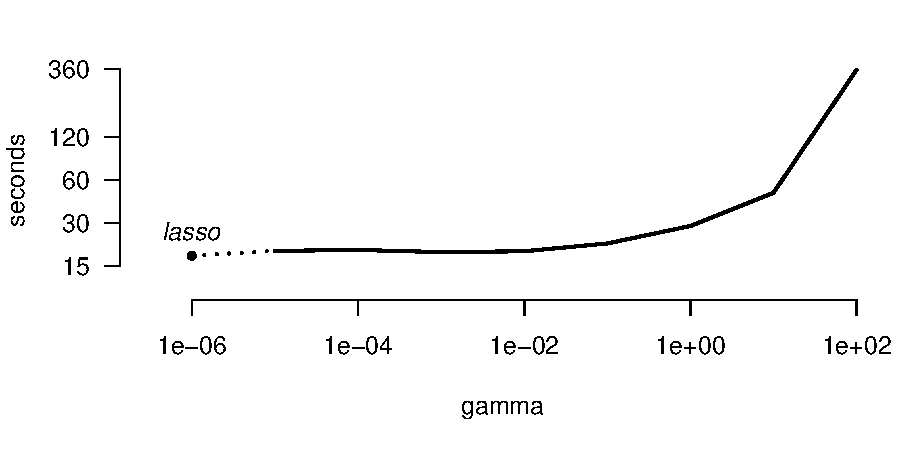
\includegraphics[width=5in]{graphs/nhl_time}
\vskip -.25cm
\caption{\label{nhltime} 
Timings for the hockey data path fits of Section 6
on a length-100 grid with $\lambda^{100} = 0.01\lambda^1$. }
\vskip -.25cm
\end{figure}



\section{Information Criteria}


We would like to choose a model that performs well in predicting new data.
 `Good prediction' can be measured in a variety of ways.  A common and
 coherent framework is to consider minimizing Kullback-Leibler (KL)
 divergence.  Say $g(\bm{y})$ is the true data generating process, and
 $f(\bm{y}; \bs{\eta},\phi)$ is the parametric density under study, which we
 suppose here is a natural exponential family  with $\ds{E}[\bm{y}]=\bs{\eta}$
 and dispersion $\phi$. Then we wish to minimize
\begin{equation}
\mr{KL}(\bs{\eta},\phi) = \ds{E}_g \log g(\bm{y}) - \ds{E}_g \log f(\bm{y}; \bs{\eta},\phi),
\end{equation}
the expected difference between log true density and our parametric approximation.  Since $\ds{E}_g \log g(\bm{y})$ is constant, this leads one to minimize 
$Q(\bs{\eta},\phi) = -\ds{E}_g \log f(\bm{y}; \bs{\eta},\phi)$, the expected negative log likelihood.   There is no requirement that $g$ is a member of the family defined by $f$.

If parameters are to be estimated as $[\bs{\eta}_{\bm{y}},\phi_{\bm{y}}]$, functions of random sample $\bm{y} \sim g$, then $Q(\bs{\eta}_{\bm{y}},\phi_{\bm{y}})$ is itself a random variable and one chooses estimators to minimize its expectation.  {\it Crucially, we imagine a double-sample expectation}, where the minimization objective is
\begin{equation}\label{dualexpect}
\ds{E}_{\bm{y}|g} \ds{E}_{\bm{\tilde y}|g} \log f(\bm{\tilde y}; \bs{\eta}_{\bm{y}},\phi_{\bm{y}}).
\end{equation}
The notation here indicates that inner and outer expectations are based on two {\it independent} random samples from $g$: $\bm{y}$ for training, upon which $\bs{\eta}_{\bm{y}},\phi_{\bm{y}}$ are calculated, and $\bm{\tilde y}$ for validation.  

Information criteria (IC) are analytic approximations to metrics like
(\ref{dualexpect}).\footnote{Not all IC target (\ref{dualexpect}).  For
example, the `Bayesian' BIC, with  $c(df) =\log(n)df$
\citep{schwarz_estimating_1978}, is derived
\citep{kass_bayes_1995} as Laplace approximation to the negative log of the
 {\it marginal likelihood}.  We include the BIC as a comparator to AIC and
 AICc in our examples. }  They take the form
\begin{equation}\label{ic}
 -2\log f(\bm{y}; \bs{\eta}_{\bm{y}},\phi_{\bm{y}}) + c(df)
 \end{equation} 
where $c(df)$ is cost of the {\it degrees-of-freedom} used in
$\bs{\eta}_{\bm{y}}$ -- e.g., for $\bm{y} \sim (\bs{\eta},\sigma^2\bm{I})$,
\citet{efron_least_2004} defines $df =
\sigma^{-2} \sum_i \mr{cov}(\eta_{\bm{y}i}, y_i)$. 

Consider a Gaussian regression model where $\bs{\eta}_\bm{y}$ is an estimate
for $\bs{\eta} = \ds{E}\bm{y}$ using $df$ degrees of freedom, and set $\phi_\bm{y} =
\sigma^2_{\bm{y}} = \sum_i (y_i - \eta_{\bm{y}i})^2/n$. We'll derive
\begin{equation}\label{aiccapprox}
df\frac{n}{n-df-1}  \approx \ds{E}_{\bm{y}|g}\left[\log f(\bm{y}; \bs{\eta}_{\bm{y}},\phi_{\bm{y}}) - \ds{E}_{\bm{\tilde y}|g} \log f(\bm{\tilde y}; \bs{\eta}_{\bm{y}},\phi_{\bm{y}})
\right],
\end{equation}
such that AICc's complexity penalty is the expected bias that results from taking the fitted log likelihood as an estimate for (\ref{dualexpect}).  First, by cancellation the inner term of (\ref{aiccapprox}) simplifies as 
\begin{equation}
\log f(\bm{y}; \bs{\eta}_{\bm{y}},\phi_{\bm{y}}) - \ds{E}_{\bm{\tilde y}|g} \log f(\bm{\tilde y}; \bs{\eta}_{\bm{y}},\phi_{\bm{y}}) = 
\frac{\ds{E}_{\bm{\tilde y}|g} \sum_i (\tilde y_i - \eta_{\bm{y}i})^2}{2 \sigma^2_{\bm{y}}} - \frac{n}{2}.
\end{equation}
Now, assume that the {\it true} model is linear and that the data were generated
from $\bm{y}\sim g(\bs{\eta}, \sigma^2\bm{I})$.  The \cite{mallows_comments_1973} $C_p$ formula holds that 
$n\sigma^2_{\bm{y}} + 2 \sigma^2 df$ is an unbiased estimator for  expected 
sum of square errors $\ds{E}_{\bm{\tilde y}|g} \sum_i (\tilde y_i - \eta_{\bm{y}i})^2/n$, such that
\begin{equation}
\frac{\ds{E}_{\bm{\tilde y}|g} \sum_i (\tilde y_i - \eta_{\bm{y}i})^2}{2 \sigma^2_{\bm{y}}} - \frac{n}{2} 
 ~\approx~ \frac{n\sigma^2_{\bm{y}} + 2 \sigma^2 df}{2 \sigma^2_{\bm{y}}} - \frac{n}{2}
 ~=~  df\frac{\sigma^2 }{\sigma^2_{\bm{y}}}.
\end{equation}
At this point, we see that the standard AIC approximation results from equating $\sigma^2 \approx \ds{E}_{\bm{y}|g}\sigma^2_{\bm{y}}$, so that $df\ds{E}_{\bm{y}|g}[\sigma^2/\sigma^2_{\bm{y}}] \approx df$.  This will underpenalize complexity whenever residual variance $\sigma^2_{\bm{y}}$ tends to be smaller than the true variance $\sigma^2$  -- that is, whenever the model is overfit.  In contrast, AICc applies the chi-squared goodness of fit result $
{n\sigma^2_{\bm{y}}/\sigma^2} \sim \chi^2_{n-df-1}
$
to obtain 
\begin{equation}
\ds{E}_{\bm{y}|g}\left[\frac{\sigma^2 }{\sigma^2_{\bm{y}}}df\right]= 
n\ds{E}_{\bm{y}|g}\left[\frac{1}{n\sigma^2_{\bm{y}}/\sigma^2}\right]df = 
\frac{n}{n-df-1}df.
\end{equation}
Multiplying by $-2$ and subtracting from $-2\log f(\bm{y}; \bs{\eta}_{\bm{y}},\sigma_{\bm{y}})$ yields the AICc.



\section{Full simulation results}

Continuous-response data are simulated from
 a $p=1000$ dimensional linear model
\begin{align}
\label{simdgp-both}
y &\sim \mr{N}\left(\bm{x}'\bs{\beta},\sigma^2\right) ~~\text{where}~~
\beta_j = (-1)^j\exp\left(-\frac{j}{{\sf d}} \right)\text{for}~~j=1\dots p~~\text{and,~given~}\bm{z} \sim \mr{N}\left(\bm{0},\bs{\Sigma}\right)\notag,\\
&\text{either}~~\textit{dense design:~~} x_j=z_j ~~\text{or}~~ \textit{sparse design:~~} 
x_j \stackrel{ind}{\sim} \mr{Bern}\left( 1/(1+e^{-z_j})\right).
\end{align}

\vspace{-.4cm}
\noindent
Each simulation draws $n=1000$ means $\eta_i =
\bm{x}_i'\bs{\beta}$, and two independent response samples 
$\bm{y},\bm{\tilde y} \sim \mr{N}(\bs{\eta},\sigma^2\bm{I})$. Residual
variance $\sigma^2$ and covariate correlation $\bs{\Sigma}$ are adjusted across
runs.  In the first case, we define $\sigma^2$ through {\it signal-to-noise}
ratios $\mr{sd}(\bs{\eta})/\sigma$ of $1/2$, $1$, and $2$.  In the latter
case, multicollinearity is parametrized via $\Sigma_{jk} =
\rho^{|j-k|}$, and we consider $\rho = 0, 0.5,~\text{and}~0.9$.
Finally, the coefficient decay rate ${\sf d}$ controls the effective sparsity: how much $\bs{\beta}$ is \textit{measurably} different from zero. See Figure \ref{fig:betadecay} for illustration; we consider
${\sf d}$ of $10$, $50$, $100$, and $200$.

\begin{figure}[h]\centering
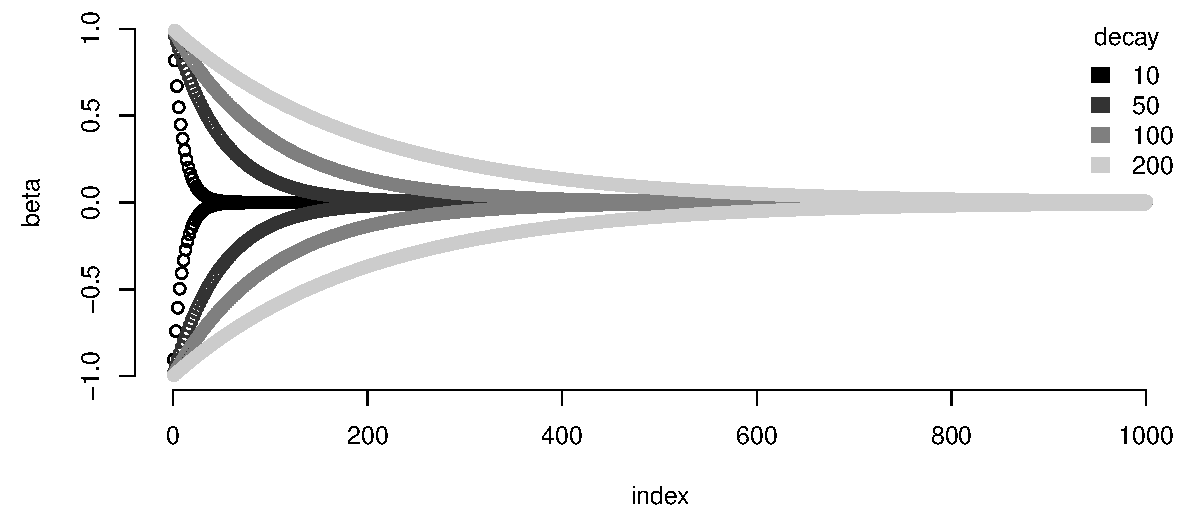
\includegraphics[width=.8\textwidth]{./graphs/betadecay}
\caption{\label{fig:betadecay} The linear model coefficients for our simulation in \ref{simdgp-both}.}
\end{figure}
% pdf("betadecay.pdf",width=8,height=3.5)
% par(mai=c(.9,.9,.1,.1))
% j <- 1:1000
% b <- function(d){ ((-1)^j)*exp(-j/d) }
% plot(j, b(10), bty="n",xlab="index",ylab="beta", ylim=c(-1,1))
% points(j, b(50), col="grey20")
% points(j, b(100), col="grey50")
% points(j, b(200), col="grey80")
% legend("topright", bty="n", fill=paste("grey",c(0,20,50,80),sep=""),legend=c(10,50,100,200),title="decay",border=0)
% dev.off()


Results for both sparse and dense designs, over a set of 1000 datasets, are presented in the following tables.  We first report out-of-sample $R^2 = 1 -
\mr{var}(\bm{\tilde y} - \bs{\eta}_\bm{y})/\mr{var}(\bm{\tilde y})$, followed by tables showing false discovery and sensitivity with respect to the $C_p$
oracle. 

\setstretch{1}
\bibliographystyle{chicago}
\bibliography{taddy}

%%!TEX root = supplemental.tex


\clearpage
\begin{table}
\vspace{-.2cm}
\footnotesize
\caption{ 
	{\bf  Predictive $\boldsymbol{R^2}$ for 100 observations, 
	binary design with dense covariates.}
  Reported as  \% worse than the Oracle 
  -- MLE fit on the $C_p$ optimal covariates -- 
  across 1000 samples.}
\begin{center}
\begin{tabular}{ccc|cc|cc|cc|cc|c|c}
\hline &&&\multicolumn{9}{|c|}{~}\\[-1ex]
\multicolumn{3}{c}{~}&\multicolumn{9}{|c|}{\bf \% Worse than Oracle } &   \\[1ex]
& &
& \multicolumn{2}{c}{lasso} 
& \multicolumn{2}{c}{GL $\gamma=1$} 
& \multicolumn{2}{c}{GL $\gamma=10$} 
& \multicolumn{2}{c}{marginal AL} 
& \multicolumn{1}{c|}{~} & \\[-0.5ex]
$\mathrm{sd}(\boldsymbol{\eta})/\sigma$ & {\sf d} & $\rho$ 
& ~~~\scriptsize\it AICc & \multicolumn{1}{c}{\scriptsize\it CV~~~}
& ~~~\scriptsize\it AICc & \multicolumn{1}{c}{\scriptsize\it CV~~~}
& ~~~\scriptsize\it AICc & \multicolumn{1}{c}{\scriptsize\it CV~~~}
& ~~~\scriptsize\it AICc & \multicolumn{1}{c}{\scriptsize\it CV~~~} 
& \multicolumn{1}{c|}{ MCP} & Oracle $R^2$ \\[.5ex]
\hline\rule{0pt}{3ex}
& & \it  0  & 35 & 22 & 30 & 26 & 17 & 47 & 19 & {\bf 14} & 25 & \it  0.73 \\
 & \it  10  & \it  0.5  & 40 & 28 & 34 & 31 & 17 & 51 & 21 & {\bf 14} & 29 & \it  0.73 \\
& & \it  0.9  & 43 & 30 & 38 & 34 & 17 & 55 & 23 & {\bf 15} & 32 & \it  0.73 \\[1ex]
\cline{2-3}\rule{0pt}{3ex}
& & \it  0  & 75 & 68 & 13 & 88 & 6 & 96 & 33 & {\bf 4} & 66 & \it  0.63 \\
\it  2  & \it  50  & \it  0.5  & 76 & 71 & 16 & 90 & 6 & 97 & 33 & {\bf 4} & 71 & \it  0.63 \\
& & \it  0.9  & 78 & 73 & 21 & 90 & 6 & 96 & 36 & {\bf 5} & 74 & \it  0.63 \\[1ex]
\cline{2-3}\rule{0pt}{3ex}
& & \it  0  & 79 & 73 & {\bf -1} & 94 & 0 & 97 & 32 & {\bf -1} & 72 & \it  0.59 \\
 & \it  100  & \it  0.5  & 79 & 75 & 0 & 94 & 0 & 98 & 33 & {\bf -1} & 76 & \it  0.60 \\
& & \it  0.9  & 80 & 76 & 2 & 94 & 0 & 98 & 35 & {\bf -1} & 76 & \it  0.60 \\[1ex]
\cline{2-3}\rule{0pt}{3ex}
& & \it  0  & 80 & 75 & {\bf -3} & 96 & -1 & 98 & 32 & {\bf -3} & 73 & \it  0.59 \\
 & \it  200  & \it  0.5  & 81 & 79 & {\bf -3} & 96 & -1 & 98 & 34 & {\bf -3} & 78 & \it  0.59 \\
& & \it  0.9  & 80 & 79 & {\bf -2} & 96 & -1 & 98 & 35 & {\bf -2} & 78 & \it  0.59 \\
\hline\rule{0pt}{3ex}
& & \it  0  & 63 & 63 & 64 & 74 & 101 & 90 & {\bf 41} & 79 & 65 & \it  0.37 \\
 & \it  10  & \it  0.5  & 65 & 66 & 67 & 76 & 99 & 91 & {\bf 43} & 79 & 69 & \it  0.37 \\
& & \it  0.9  & 67 & 68 & 69 & 77 & 98 & 90 & {\bf 45} & 78 & 70 & \it  0.37 \\[1ex]
\cline{2-3}\rule{0pt}{3ex}
& & \it  0  & 70 & 72 & 62 & 97 & 108 & 103 & {\bf 21} & 75 & 75 & \it  0.20 \\
\it  1  & \it  50  & \it  0.5  & 72 & 78 & 59 & 98 & 106 & 104 & {\bf 22} & 74 & 81 & \it  0.20 \\
& & \it  0.9  & 75 & 79 & 61 & 97 & 106 & 102 & {\bf 27} & 72 & 80 & \it  0.20 \\[1ex]
\cline{2-3}\rule{0pt}{3ex}
& & \it  0  & 57 & 60 & 65 & 102 & 117 & 107 & {\bf -29} & 59 & 62 & \it  0.12 \\
 & \it  100  & \it  0.5  & 63 & 69 & 60 & 102 & 113 & 107 & {\bf -23} & 57 & 73 & \it  0.12 \\
& & \it  0.9  & 59 & 64 & 58 & 100 & 113 & 106 & {\bf -23} & 53 & 65 & \it  0.12 \\[1ex]
\cline{2-3}\rule{0pt}{3ex}
& & \it  0  & 7 & 13 & 50 & 109 & 141 & 117 & {\bf -201} & 7 & 15 & \it  0.05 \\
 & \it  200  & \it  0.5  & 18 & 32 & 45 & 108 & 126 & 116 & {\bf -164} & 7 & 42 & \it  0.06 \\
& & \it  0.9  & 3 & 16 & 44 & 104 & 130 & 114 & {\bf -184} & -8 & 24 & \it  0.05 \\
\hline\rule{0pt}{3ex}
& & \it  0  & {\bf 115} & 142 & 720 & 149 & 1483 & 152 & 281 & 1198 & 161 & \it  0.04 \\
 & \it  10  & \it  0.5  & {\bf 116} & 141 & 633 & 149 & 1450 & 151 & 287 & 1186 & 158 & \it  0.05 \\
& & \it  0.9  & {\bf 114} & 147 & 623 & 148 & 1471 & 152 & 295 & 1171 & 156 & \it  0.04 \\[1ex]
\cline{2-3}\rule{0pt}{3ex}
& & \it  0  & {\bf -74} & -56 & 969 & -53 & 1162 & -49 & 81 & 915 & -49 & \it  -0.05 \\
\it  0.5  & \it  50  & \it  0.5  & {\bf -73} & -56 & 972 & -53 & 1183 & -52 & 72 & 920 & -47 & \it  -0.05 \\
& & \it  0.9  & {\bf -81} & -53 & 979 & -56 & 1206 & -51 & 82 & 909 & -47 & \it  -0.05 \\[1ex]
\cline{2-3}\rule{0pt}{3ex}
& & \it  0  & {\bf -81} & -66 & 827 & -63 & 929 & -61 & 47 & 724 & -56 & \it  -0.06 \\
 & \it  100  & \it  0.5  & {\bf -80} & -64 & 824 & -60 & 939 & -61 & 46 & 730 & -57 & \it  -0.06 \\
& & \it  0.9  & {\bf -85} & -68 & 822 & -63 & 945 & -62 & 49 & 707 & -61 & \it  -0.06 \\[1ex]
\cline{2-3}\rule{0pt}{3ex}
& & \it  0  & {\bf -80} & -65 & 843 & -62 & 907 & -60 & 43 & 706 & -57 & \it  -0.06 \\
 & \it  200  & \it  0.5  & {\bf -80} & -65 & 854 & -62 & 926 & -62 & 42 & 716 & -58 & \it  -0.06 \\
& & \it  0.9  & {\bf -86} & -71 & 822 & -66 & 896 & -65 & 44 & 670 & -61 & \it  -0.06 \\
\hline\end{tabular}
\end{center}
\end{table}




\clearpage
\begin{table}
\vspace{-.2cm}
\footnotesize
\caption{ 
	{\bf  Predictive $\boldsymbol{R^2}$ for 100 observations, 
	continuous design with dense covariates.}
  Reported as  \% worse than the Oracle 
  -- MLE fit on the $C_p$ optimal covariates -- 
  across 1000 samples.}
\begin{center}
\begin{tabular}{ccc|cc|cc|cc|cc|c|c}
\hline &&&\multicolumn{9}{|c|}{~}\\[-1ex]
\multicolumn{3}{c}{~}&\multicolumn{9}{|c|}{\bf \% Worse than Oracle } &   \\[1ex]
& &
& \multicolumn{2}{c}{lasso} 
& \multicolumn{2}{c}{GL $\gamma=1$} 
& \multicolumn{2}{c}{GL $\gamma=10$} 
& \multicolumn{2}{c}{marginal AL} 
& \multicolumn{1}{c|}{~} & \\[-0.5ex]
$\mathrm{sd}(\boldsymbol{\eta})/\sigma$ & {\sf d} & $\rho$ 
& ~~~\scriptsize\it AICc & \multicolumn{1}{c}{\scriptsize\it CV~~~}
& ~~~\scriptsize\it AICc & \multicolumn{1}{c}{\scriptsize\it CV~~~}
& ~~~\scriptsize\it AICc & \multicolumn{1}{c}{\scriptsize\it CV~~~}
& ~~~\scriptsize\it AICc & \multicolumn{1}{c}{\scriptsize\it CV~~~} 
& \multicolumn{1}{c|}{ MCP} & Oracle $R^2$ \\[.5ex]
\hline\rule{0pt}{3ex}
& & \it  0  & 35 & 24 & 46 & 28 & 18 & 48 & 19 & {\bf 13} & 26 & \it  0.73 \\
 & \it  10  & \it  0.5  & 66 & 64 & 81 & 65 & 29 & 73 & 39 & {\bf 18} & 57 & \it  0.74 \\
& & \it  0.9  & 40 & 41 & 47 & 41 & 44 & 41 & 23 & {\bf 18} & 40 & \it  0.74 \\[1ex]
\cline{2-3}\rule{0pt}{3ex}
& & \it  0  & 74 & 68 & 61 & 89 & 6 & 96 & 31 & {\bf 4} & 68 & \it  0.63 \\
\it  2  & \it  50  & \it  0.5  & 83 & 85 & 96 & 93 & {\bf 6} & 98 & 43 & 7 & 85 & \it  0.64 \\
& & \it  0.9  & 71 & 75 & 90 & 76 & 51 & 83 & 48 & {\bf 36} & 74 & \it  0.64 \\[1ex]
\cline{2-3}\rule{0pt}{3ex}
& & \it  0  & 78 & 72 & 22 & 94 & 0 & 97 & 31 & {\bf -2} & 73 & \it  0.59 \\
 & \it  100  & \it  0.5  & 85 & 86 & 85 & 95 & {\bf 0} & 99 & 40 & 1 & 86 & \it  0.59 \\
& & \it  0.9  & 79 & 84 & 97 & 87 & {\bf 9} & 94 & 50 & 35 & 84 & \it  0.60 \\[1ex]
\cline{2-3}\rule{0pt}{3ex}
& & \it  0  & 80 & 75 & 2 & 96 & -1 & 98 & 32 & {\bf -3} & 76 & \it  0.59 \\
 & \it  200  & \it  0.5  & 84 & 87 & 53 & 96 & {\bf -1} & 99 & 39 & 0 & 86 & \it  0.59 \\
& & \it  0.9  & 84 & 88 & 99 & 92 & {\bf -1} & 98 & 53 & 36 & 88 & \it  0.59 \\
\hline\rule{0pt}{3ex}
& & \it  0  & 61 & 64 & 87 & 73 & 100 & 88 & {\bf 40} & 78 & 64 & \it  0.37 \\
 & \it  10  & \it  0.5  & 76 & 79 & 92 & 82 & 95 & 90 & {\bf 53} & 77 & 78 & \it  0.37 \\
& & \it  0.9  & 40 & 42 & 49 & 40 & 42 & 37 & {\bf 33} & 38 & 35 & \it  0.39 \\[1ex]
\cline{2-3}\rule{0pt}{3ex}
& & \it  0  & 70 & 74 & 77 & 96 & 105 & 102 & {\bf 20} & 73 & 74 & \it  0.20 \\
\it  1  & \it  50  & \it  0.5  & 80 & 87 & 97 & 96 & 104 & 104 & {\bf 32} & 67 & 85 & \it  0.20 \\
& & \it  0.9  & 68 & 76 & 95 & 78 & 93 & 92 & 40 & {\bf 36} & 75 & \it  0.22 \\[1ex]
\cline{2-3}\rule{0pt}{3ex}
& & \it  0  & 56 & 64 & 63 & 100 & 112 & 107 & {\bf -29} & 54 & 66 & \it  0.12 \\
 & \it  100  & \it  0.5  & 67 & 77 & 79 & 98 & 110 & 107 & {\bf -14} & 42 & 78 & \it  0.12 \\
& & \it  0.9  & 68 & 79 & 102 & 87 & 99 & 101 & 17 & {\bf 8} & 79 & \it  0.13 \\[1ex]
\cline{2-3}\rule{0pt}{3ex}
& & \it  0  & 9 & 27 & 53 & 104 & 132 & 115 & {\bf -184} & 1 & 27 & \it  0.05 \\
 & \it  200  & \it  0.5  & 31 & 49 & 26 & 104 & 125 & 116 & {\bf -146} & -33 & 51 & \it  0.05 \\
& & \it  0.9  & 42 & 67 & 108 & 87 & 111 & 109 & -62 & {\bf -85} & 69 & \it  0.06 \\
\hline\rule{0pt}{3ex}
& & \it  0  & {\bf 106} & 135 & 282 & 137 & 1311 & 146 & 242 & 1054 & 141 & \it  0.05 \\
 & \it  10  & \it  0.5  & {\bf 114} & 127 & 131 & 127 & 1220 & 139 & 249 & 924 & 137 & \it  0.05 \\
& & \it  0.9  & {\bf 66} & 79 & 90 & 77 & 560 & 93 & 125 & 233 & 79 & \it  0.08 \\[1ex]
\cline{2-3}\rule{0pt}{3ex}
& & \it  0  & {\bf -81} & -56 & 962 & -55 & 1224 & -51 & 74 & 956 & -41 & \it  -0.05 \\
\it  0.5  & \it  50  & \it  0.5  & {\bf -77} & -56 & 396 & -54 & 1288 & -49 & 86 & 881 & -51 & \it  -0.04 \\
& & \it  0.9  & {\bf -68} & -41 & -36 & -28 & 2652 & 0 & 210 & 549 & -24 & \it  -0.02 \\[1ex]
\cline{2-3}\rule{0pt}{3ex}
& & \it  0  & {\bf -83} & -66 & 857 & -62 & 969 & -59 & 44 & 745 & -57 & \it  -0.06 \\
 & \it  100  & \it  0.5  & {\bf -79} & -62 & 638 & -62 & 997 & -62 & 50 & 678 & -63 & \it  -0.06 \\
& & \it  0.9  & {\bf -71} & -65 & -61 & -56 & 1311 & -49 & 57 & 241 & -56 & \it  -0.04 \\[1ex]
\cline{2-3}\rule{0pt}{3ex}
& & \it  0  & {\bf -86} & -70 & 846 & -66 & 907 & -62 & 34 & 703 & -61 & \it  -0.06 \\
 & \it  200  & \it  0.5  & {\bf -80} & -66 & 775 & -65 & 931 & -65 & 43 & 624 & -66 & \it  -0.06 \\
& & \it  0.9  & {\bf -74} & -71 & -34 & -61 & 1050 & -57 & 34 & 173 & -65 & \it  -0.05 \\
\hline\end{tabular}
\end{center}
\end{table}




\clearpage
\begin{table}
\vspace{-.2cm}
\footnotesize
\caption{ 
	{\bf  Predictive $\boldsymbol{R^2}$ for 100 observations, 
	binary design with sparse covariates.}
  Reported as  \% worse than the Oracle 
  -- MLE fit on the true nonzero covariates -- 
  across 1000 samples.}
\begin{center}
\begin{tabular}{ccc|cc|cc|cc|cc|c|c}
\hline &&&\multicolumn{9}{|c|}{~}\\[-1ex]
\multicolumn{3}{c}{~}&\multicolumn{9}{|c|}{\bf \% Worse than Oracle } &   \\[1ex]
& &
& \multicolumn{2}{c}{lasso} 
& \multicolumn{2}{c}{GL $\gamma=1$} 
& \multicolumn{2}{c}{GL $\gamma=10$} 
& \multicolumn{2}{c}{marginal AL} 
& \multicolumn{1}{c|}{~} & \\[-0.5ex]
$\mathrm{sd}(\boldsymbol{\eta})/\sigma$ & {\sf d} & $\rho$ 
& ~~~\scriptsize\it AICc & \multicolumn{1}{c}{\scriptsize\it CV~~~}
& ~~~\scriptsize\it AICc & \multicolumn{1}{c}{\scriptsize\it CV~~~}
& ~~~\scriptsize\it AICc & \multicolumn{1}{c}{\scriptsize\it CV~~~}
& ~~~\scriptsize\it AICc & \multicolumn{1}{c}{\scriptsize\it CV~~~} 
& \multicolumn{1}{c|}{ MCP} & Oracle $R^2$ \\[.5ex]
\hline\rule{0pt}{3ex}
& & \it  0  & 23 & 17 & 17 & 14 & 20 & 20 & 14 & 15 & {\bf 13} & \it  0.77 \\
 & \it  10  & \it  0.5  & 28 & 19 & 20 & 17 & 20 & 26 & 17 & 16 & {\bf 15} & \it  0.77 \\
& & \it  0.9  & 30 & 20 & 22 & 19 & 20 & 29 & 19 & {\bf 16} & 17 & \it  0.77 \\[1ex]
\cline{2-3}\rule{0pt}{3ex}
& & \it  0  & 26 & 18 & {\bf 14} & 17 & 21 & 42 & 16 & 16 & 16 & \it  0.77 \\
\it  2  & \it  50  & \it  0.5  & 34 & 23 & {\bf 17} & 23 & 21 & 53 & 19 & {\bf 17} & 21 & \it  0.77 \\
& & \it  0.9  & 37 & 25 & 20 & 27 & 21 & 57 & 22 & {\bf 17} & 23 & \it  0.77 \\[1ex]
\cline{2-3}\rule{0pt}{3ex}
& & \it  0  & 26 & 18 & {\bf 14} & 17 & 21 & 45 & 16 & 16 & 17 & \it  0.77 \\
 & \it  100  & \it  0.5  & 34 & 24 & {\bf 16} & 24 & 21 & 55 & 19 & 17 & 21 & \it  0.77 \\
& & \it  0.9  & 37 & 25 & 19 & 28 & 21 & 59 & 21 & {\bf 17} & 23 & \it  0.77 \\[1ex]
\cline{2-3}\rule{0pt}{3ex}
& & \it  0  & 26 & 19 & {\bf 13} & 17 & 21 & 44 & 16 & 16 & 17 & \it  0.77 \\
 & \it  200  & \it  0.5  & 34 & 24 & {\bf 16} & 24 & 21 & 55 & 19 & 17 & 21 & \it  0.77 \\
& & \it  0.9  & 37 & 25 & 19 & 29 & 21 & 59 & 21 & {\bf 17} & 23 & \it  0.77 \\
\hline\rule{0pt}{3ex}
& & \it  0  & 59 & 59 & 61 & 67 & 99 & 83 & {\bf 43} & 79 & 62 & \it  0.43 \\
 & \it  10  & \it  0.5  & 63 & 65 & 66 & 70 & 98 & 86 & {\bf 47} & 81 & 66 & \it  0.43 \\
& & \it  0.9  & 65 & 65 & 67 & 71 & 98 & 87 & {\bf 48} & 79 & 67 & \it  0.43 \\[1ex]
\cline{2-3}\rule{0pt}{3ex}
& & \it  0  & 68 & 67 & 68 & 81 & 102 & 94 & {\bf 48} & 83 & 69 & \it  0.43 \\
\it  1  & \it  50  & \it  0.5  & 72 & 73 & 70 & 85 & 101 & 95 & {\bf 52} & 84 & 75 & \it  0.43 \\
& & \it  0.9  & 74 & 74 & 71 & 85 & 100 & 96 & {\bf 54} & 82 & 75 & \it  0.43 \\[1ex]
\cline{2-3}\rule{0pt}{3ex}
& & \it  0  & 68 & 67 & 68 & 82 & 102 & 95 & {\bf 49} & 83 & 69 & \it  0.43 \\
 & \it  100  & \it  0.5  & 72 & 73 & 70 & 85 & 101 & 96 & {\bf 52} & 84 & 76 & \it  0.43 \\
& & \it  0.9  & 74 & 74 & 71 & 86 & 101 & 96 & {\bf 54} & 82 & 76 & \it  0.43 \\[1ex]
\cline{2-3}\rule{0pt}{3ex}
& & \it  0  & 68 & 67 & 68 & 82 & 102 & 95 & {\bf 49} & 83 & 69 & \it  0.43 \\
 & \it  200  & \it  0.5  & 73 & 74 & 70 & 86 & 102 & 96 & {\bf 52} & 84 & 75 & \it  0.43 \\
& & \it  0.9  & 75 & 74 & 71 & 86 & 101 & 96 & {\bf 54} & 82 & 76 & \it  0.43 \\
\hline\rule{0pt}{3ex}
& & \it  0  & {\bf 106} & 117 & 345 & 121 & 734 & 126 & 180 & 598 & 126 & \it  0.10 \\
 & \it  10  & \it  0.5  & {\bf 106} & 120 & 319 & 120 & 740 & 123 & 182 & 613 & 126 & \it  0.10 \\
& & \it  0.9  & {\bf 106} & 118 & 286 & 120 & 714 & 124 & 181 & 579 & 124 & \it  0.10 \\[1ex]
\cline{2-3}\rule{0pt}{3ex}
& & \it  0  & {\bf 109} & 117 & 526 & 122 & 744 & 126 & 182 & 611 & 129 & \it  0.10 \\
\it  0.5  & \it  50  & \it  0.5  & {\bf 108} & 121 & 506 & 122 & 748 & 125 & 183 & 616 & 127 & \it  0.10 \\
& & \it  0.9  & {\bf 108} & 120 & 489 & 122 & 734 & 124 & 189 & 593 & 127 & \it  0.10 \\[1ex]
\cline{2-3}\rule{0pt}{3ex}
& & \it  0  & {\bf 109} & 118 & 550 & 123 & 752 & 127 & 187 & 616 & 130 & \it  0.10 \\
 & \it  100  & \it  0.5  & {\bf 108} & 124 & 533 & 122 & 753 & 125 & 185 & 619 & 127 & \it  0.10 \\
& & \it  0.9  & {\bf 107} & 121 & 511 & 122 & 740 & 124 & 188 & 597 & 126 & \it  0.10 \\[1ex]
\cline{2-3}\rule{0pt}{3ex}
& & \it  0  & {\bf 109} & 117 & 551 & 122 & 748 & 127 & 184 & 612 & 129 & \it  0.10 \\
 & \it  200  & \it  0.5  & {\bf 108} & 124 & 542 & 122 & 759 & 125 & 185 & 624 & 129 & \it  0.09 \\
& & \it  0.9  & {\bf 108} & 123 & 523 & 124 & 743 & 123 & 189 & 600 & 126 & \it  0.10 \\
\hline\end{tabular}
\end{center}
\end{table}




\clearpage
\begin{table}
\vspace{-.2cm}
\footnotesize
\caption{ 
	{\bf  Predictive $\boldsymbol{R^2}$ for 100 observations, 
	continuous design with sparse covariates.}
  Reported as  \% worse than the Oracle 
  -- MLE fit on the true nonzero covariates -- 
  across 1000 samples.}
\begin{center}
\begin{tabular}{ccc|cc|cc|cc|cc|c|c}
\hline &&&\multicolumn{9}{|c|}{~}\\[-1ex]
\multicolumn{3}{c}{~}&\multicolumn{9}{|c|}{\bf \% Worse than Oracle } &   \\[1ex]
& &
& \multicolumn{2}{c}{lasso} 
& \multicolumn{2}{c}{GL $\gamma=1$} 
& \multicolumn{2}{c}{GL $\gamma=10$} 
& \multicolumn{2}{c}{marginal AL} 
& \multicolumn{1}{c|}{~} & \\[-0.5ex]
$\mathrm{sd}(\boldsymbol{\eta})/\sigma$ & {\sf d} & $\rho$ 
& ~~~\scriptsize\it AICc & \multicolumn{1}{c}{\scriptsize\it CV~~~}
& ~~~\scriptsize\it AICc & \multicolumn{1}{c}{\scriptsize\it CV~~~}
& ~~~\scriptsize\it AICc & \multicolumn{1}{c}{\scriptsize\it CV~~~}
& ~~~\scriptsize\it AICc & \multicolumn{1}{c}{\scriptsize\it CV~~~} 
& \multicolumn{1}{c|}{ MCP} & Oracle $R^2$ \\[.5ex]
\hline\rule{0pt}{3ex}
& & \it  0  & 23 & 17 & 23 & 15 & 21 & 22 & 15 & 15 & {\bf 14} & \it  0.78 \\
 & \it  10  & \it  0.5  & 61 & 58 & 74 & 57 & 36 & 65 & 39 & {\bf 22} & 49 & \it  0.77 \\
& & \it  0.9  & 45 & 45 & 55 & 45 & 53 & 46 & 29 & {\bf 22} & 42 & \it  0.77 \\[1ex]
\cline{2-3}\rule{0pt}{3ex}
& & \it  0  & 26 & 18 & 22 & 17 & 20 & 38 & 16 & {\bf 15} & 16 & \it  0.77 \\
\it  2  & \it  50  & \it  0.5  & 71 & 70 & 88 & 74 & 23 & 86 & 43 & {\bf 22} & 68 & \it  0.77 \\
& & \it  0.9  & 55 & 53 & 72 & 53 & 62 & 56 & 41 & {\bf 32} & 51 & \it  0.78 \\[1ex]
\cline{2-3}\rule{0pt}{3ex}
& & \it  0  & 26 & 18 & 21 & 17 & 21 & 41 & 16 & {\bf 15} & 16 & \it  0.77 \\
 & \it  100  & \it  0.5  & 72 & 70 & 88 & 75 & 23 & 87 & 43 & {\bf 22} & 69 & \it  0.77 \\
& & \it  0.9  & 56 & 53 & 73 & 53 & 61 & 57 & 41 & {\bf 33} & 52 & \it  0.77 \\[1ex]
\cline{2-3}\rule{0pt}{3ex}
& & \it  0  & 26 & 18 & 21 & 17 & 21 & 39 & 16 & {\bf 15} & 16 & \it  0.77 \\
 & \it  200  & \it  0.5  & 72 & 70 & 89 & 75 & 23 & 87 & 43 & {\bf 22} & 69 & \it  0.78 \\
& & \it  0.9  & 56 & 53 & 73 & 53 & 59 & 57 & 41 & {\bf 33} & 52 & \it  0.78 \\
\hline\rule{0pt}{3ex}
& & \it  0  & 58 & 60 & 79 & 66 & 98 & 83 & {\bf 43} & 77 & 62 & \it  0.44 \\
 & \it  10  & \it  0.5  & 75 & 78 & 90 & 81 & 94 & 88 & {\bf 57} & 79 & 77 & \it  0.44 \\
& & \it  0.9  & 52 & 55 & 64 & 54 & 59 & 52 & {\bf 45} & 49 & 49 & \it  0.44 \\[1ex]
\cline{2-3}\rule{0pt}{3ex}
& & \it  0  & 66 & 67 & 87 & 80 & 100 & 93 & {\bf 47} & 80 & 69 & \it  0.44 \\
\it  1  & \it  50  & \it  0.5  & 83 & 86 & 97 & 91 & 98 & 98 & {\bf 62} & 81 & 86 & \it  0.44 \\
& & \it  0.9  & 72 & 75 & 91 & 75 & 88 & 83 & {\bf 58} & {\bf 58} & 72 & \it  0.44 \\[1ex]
\cline{2-3}\rule{0pt}{3ex}
& & \it  0  & 67 & 67 & 86 & 81 & 100 & 94 & {\bf 48} & 80 & 68 & \it  0.44 \\
 & \it  100  & \it  0.5  & 84 & 86 & 97 & 92 & 99 & 98 & {\bf 62} & 81 & 86 & \it  0.44 \\
& & \it  0.9  & 73 & 76 & 93 & 76 & 89 & 84 & {\bf 59} & {\bf 59} & 73 & \it  0.44 \\[1ex]
\cline{2-3}\rule{0pt}{3ex}
& & \it  0  & 67 & 67 & 86 & 81 & 101 & 93 & {\bf 48} & 79 & 69 & \it  0.44 \\
 & \it  200  & \it  0.5  & 84 & 87 & 97 & 92 & 99 & 98 & {\bf 62} & 81 & 86 & \it  0.44 \\
& & \it  0.9  & 73 & 77 & 93 & 77 & 89 & 85 & {\bf 59} & {\bf 59} & 73 & \it  0.44 \\
\hline\rule{0pt}{3ex}
& & \it  0  & {\bf 102} & 114 & 162 & 117 & 706 & 124 & 167 & 575 & 120 & \it  0.10 \\
 & \it  10  & \it  0.5  & {\bf 105} & 115 & 115 & 116 & 692 & 121 & 175 & 531 & 119 & \it  0.10 \\
& & \it  0.9  & {\bf 82} & 92 & 99 & 92 & 463 & 102 & 133 & 213 & 92 & \it  0.10 \\[1ex]
\cline{2-3}\rule{0pt}{3ex}
& & \it  0  & {\bf 105} & 118 & 321 & 122 & 716 & 125 & 173 & 587 & 123 & \it  0.10 \\
\it  0.5  & \it  50  & \it  0.5  & {\bf 108} & 117 & 134 & 119 & 706 & 123 & 178 & 538 & 122 & \it  0.10 \\
& & \it  0.9  & {\bf 103} & 111 & 113 & 115 & 662 & 120 & 156 & 241 & 115 & \it  0.10 \\[1ex]
\cline{2-3}\rule{0pt}{3ex}
& & \it  0  & {\bf 105} & 117 & 354 & 122 & 718 & 125 & 174 & 589 & 124 & \it  0.10 \\
 & \it  100  & \it  0.5  & {\bf 108} & 117 & 141 & 119 & 703 & 123 & 177 & 535 & 122 & \it  0.10 \\
& & \it  0.9  & {\bf 106} & 111 & 113 & 115 & 673 & 120 & 158 & 243 & 115 & \it  0.10 \\[1ex]
\cline{2-3}\rule{0pt}{3ex}
& & \it  0  & {\bf 105} & 118 & 368 & 122 & 716 & 125 & 174 & 589 & 125 & \it  0.10 \\
 & \it  200  & \it  0.5  & {\bf 108} & 117 & 147 & 119 & 705 & 123 & 177 & 534 & 121 & \it  0.10 \\
& & \it  0.9  & {\bf 106} & 112 & 113 & 116 & 674 & 121 & 159 & 243 & 115 & \it  0.10 \\
\hline\end{tabular}
\end{center}
\end{table}




\clearpage
\begin{table}
\vspace{-.2cm}
\footnotesize
\caption{ 
	{\bf  Predictive $\boldsymbol{R^2}$ for 1000 observations, 
	binary design with dense covariates.}
  Reported as  \% worse than the Oracle 
  -- MLE fit on the $C_p$ optimal covariates -- 
  across 1000 samples.}
\begin{center}
\begin{tabular}{ccc|cc|cc|cc|cc|c|c}
\hline &&&\multicolumn{9}{|c|}{~}\\[-1ex]
\multicolumn{3}{c}{~}&\multicolumn{9}{|c|}{\bf \% Worse than Oracle } &   \\[1ex]
& &
& \multicolumn{2}{c}{lasso} 
& \multicolumn{2}{c}{GL $\gamma=1$} 
& \multicolumn{2}{c}{GL $\gamma=10$} 
& \multicolumn{2}{c}{marginal AL} 
& \multicolumn{1}{c|}{~} & \\[-0.5ex]
$\mathrm{sd}(\boldsymbol{\eta})/\sigma$ & {\sf d} & $\rho$ 
& ~~~\scriptsize\it AICc & \multicolumn{1}{c}{\scriptsize\it CV~~~}
& ~~~\scriptsize\it AICc & \multicolumn{1}{c}{\scriptsize\it CV~~~}
& ~~~\scriptsize\it AICc & \multicolumn{1}{c}{\scriptsize\it CV~~~}
& ~~~\scriptsize\it AICc & \multicolumn{1}{c}{\scriptsize\it CV~~~} 
& \multicolumn{1}{c|}{ MCP} & Oracle $R^2$ \\[.5ex]
\hline\rule{0pt}{3ex}
& & \it  0  & 3 & 3 & 2 & 2 & {\bf 1} & {\bf 1} & 2 & 2 & {\bf 1} & \it  0.79 \\
 & \it  10  & \it  0.5  & 3 & 3 & 2 & 2 & 2 & {\bf 1} & 2 & 2 & {\bf 1} & \it  0.79 \\
& & \it  0.9  & 3 & 3 & 2 & 2 & 2 & 2 & 2 & 2 & {\bf 1} & \it  0.79 \\[1ex]
\cline{2-3}\rule{0pt}{3ex}
& & \it  0  & 6 & 5 & 5 & {\bf 4} & 5 & 5 & 5 & 5 & {\bf 4} & \it  0.77 \\
\it  2  & \it  50  & \it  0.5  & 7 & 5 & 5 & 5 & 5 & 5 & 6 & 6 & {\bf 4} & \it  0.77 \\
& & \it  0.9  & 7 & 5 & 5 & 5 & 5 & 5 & 6 & 6 & {\bf 4} & \it  0.77 \\[1ex]
\cline{2-3}\rule{0pt}{3ex}
& & \it  0  & 9 & 6 & 7 & {\bf 5} & 7 & 7 & 8 & 7 & {\bf 5} & \it  0.75 \\
 & \it  100  & \it  0.5  & 10 & {\bf 6} & 8 & {\bf 6} & 7 & 8 & 9 & 8 & {\bf 6} & \it  0.75 \\
& & \it  0.9  & 10 & {\bf 6} & 8 & {\bf 6} & 7 & 7 & 9 & 8 & {\bf 6} & \it  0.75 \\[1ex]
\cline{2-3}\rule{0pt}{3ex}
& & \it  0  & 15 & 5 & 10 & 6 & 8 & 12 & 11 & 7 & {\bf 4} & \it  0.71 \\
 & \it  200  & \it  0.5  & 18 & {\bf 5} & 11 & 6 & 8 & 13 & 13 & 9 & {\bf 5} & \it  0.71 \\
& & \it  0.9  & 18 & {\bf 5} & 11 & 6 & 8 & 13 & 14 & 9 & {\bf 5} & \it  0.71 \\
\hline\rule{0pt}{3ex}
& & \it  0  & 8 & 8 & 7 & 7 & 9 & {\bf 5} & 9 & 10 & {\bf 5} & \it  0.48 \\
 & \it  10  & \it  0.5  & 9 & 9 & 7 & 7 & 9 & {\bf 6} & 9 & 10 & {\bf 6} & \it  0.48 \\
& & \it  0.9  & 10 & 10 & 8 & 8 & 9 & {\bf 6} & 10 & 10 & {\bf 6} & \it  0.48 \\[1ex]
\cline{2-3}\rule{0pt}{3ex}
& & \it  0  & 19 & 17 & {\bf 16} & 17 & 31 & 23 & 17 & 18 & 17 & \it  0.44 \\
\it  1  & \it  50  & \it  0.5  & 21 & 19 & {\bf 18} & {\bf 18} & 30 & 24 & 19 & 20 & {\bf 18} & \it  0.44 \\
& & \it  0.9  & 22 & 19 & {\bf 18} & {\bf 18} & 30 & 25 & 20 & 20 & 19 & \it  0.44 \\[1ex]
\cline{2-3}\rule{0pt}{3ex}
& & \it  0  & 26 & {\bf 21} & 22 & 25 & 41 & 52 & 22 & 22 & {\bf 21} & \it  0.40 \\
 & \it  100  & \it  0.5  & 29 & {\bf 23} & 24 & 27 & 41 & 57 & 25 & 25 & {\bf 23} & \it  0.40 \\
& & \it  0.9  & 30 & {\bf 23} & 24 & 27 & 41 & 58 & 26 & 25 & {\bf 23} & \it  0.40 \\[1ex]
\cline{2-3}\rule{0pt}{3ex}
& & \it  0  & 35 & {\bf 21} & 25 & 46 & 47 & 94 & 24 & {\bf 21} & {\bf 21} & \it  0.34 \\
 & \it  200  & \it  0.5  & 41 & 26 & 27 & 55 & 48 & 96 & 27 & {\bf 24} & 25 & \it  0.34 \\
& & \it  0.9  & 41 & 26 & 27 & 54 & 47 & 96 & 28 & {\bf 25} & 26 & \it  0.34 \\
\hline\rule{0pt}{3ex}
& & \it  0  & 27 & 27 & {\bf 23} & 24 & 52 & 24 & 43 & 55 & {\bf 23} & \it  0.17 \\
 & \it  10  & \it  0.5  & 29 & 30 & 25 & 26 & 53 & 26 & 45 & 58 & {\bf 24} & \it  0.17 \\
& & \it  0.9  & 30 & 30 & 26 & 26 & 55 & 28 & 46 & 57 & {\bf 25} & \it  0.17 \\[1ex]
\cline{2-3}\rule{0pt}{3ex}
& & \it  0  & {\bf 54} & 56 & 60 & 72 & 145 & 94 & 72 & 91 & 57 & \it  0.13 \\
\it  0.5  & \it  50  & \it  0.5  & {\bf 60} & 63 & 64 & 77 & 154 & 96 & 78 & 96 & 65 & \it  0.13 \\
& & \it  0.9  & {\bf 61} & 65 & 64 & 78 & 146 & 96 & 79 & 96 & 66 & \it  0.13 \\[1ex]
\cline{2-3}\rule{0pt}{3ex}
& & \it  0  & {\bf 62} & 69 & 87 & 93 & 150 & 101 & 85 & 113 & 68 & \it  0.09 \\
 & \it  100  & \it  0.5  & {\bf 69} & 76 & 89 & 95 & 158 & 101 & 91 & 119 & 77 & \it  0.09 \\
& & \it  0.9  & {\bf 71} & 78 & 90 & 96 & 154 & 101 & 93 & 119 & 78 & \it  0.09 \\[1ex]
\cline{2-3}\rule{0pt}{3ex}
& & \it  0  & {\bf 53} & 65 & 163 & 101 & 156 & 104 & 100 & 158 & 66 & \it  0.04 \\
 & \it  200  & \it  0.5  & {\bf 65} & 75 & 156 & 101 & 162 & 104 & 109 & 169 & 76 & \it  0.04 \\
& & \it  0.9  & {\bf 68} & 78 & 155 & 101 & 160 & 104 & 114 & 167 & 80 & \it  0.04 \\
\hline\end{tabular}
\end{center}
\end{table}




\clearpage
\begin{table}
\vspace{-.2cm}
\footnotesize
\caption{ 
	{\bf  Predictive $\boldsymbol{R^2}$ for 1000 observations, 
	continuous design with dense covariates.}
  Reported as  \% worse than the Oracle 
  -- MLE fit on the $C_p$ optimal covariates -- 
  across 1000 samples.}
\begin{center}
\begin{tabular}{ccc|cc|cc|cc|cc|c|c}
\hline &&&\multicolumn{9}{|c|}{~}\\[-1ex]
\multicolumn{3}{c}{~}&\multicolumn{9}{|c|}{\bf \% Worse than Oracle } &   \\[1ex]
& &
& \multicolumn{2}{c}{lasso} 
& \multicolumn{2}{c}{GL $\gamma=1$} 
& \multicolumn{2}{c}{GL $\gamma=10$} 
& \multicolumn{2}{c}{marginal AL} 
& \multicolumn{1}{c|}{~} & \\[-0.5ex]
$\mathrm{sd}(\boldsymbol{\eta})/\sigma$ & {\sf d} & $\rho$ 
& ~~~\scriptsize\it AICc & \multicolumn{1}{c}{\scriptsize\it CV~~~}
& ~~~\scriptsize\it AICc & \multicolumn{1}{c}{\scriptsize\it CV~~~}
& ~~~\scriptsize\it AICc & \multicolumn{1}{c}{\scriptsize\it CV~~~}
& ~~~\scriptsize\it AICc & \multicolumn{1}{c}{\scriptsize\it CV~~~} 
& \multicolumn{1}{c|}{ MCP} & Oracle $R^2$ \\[.5ex]
\hline\rule{0pt}{3ex}
& & \it  0  & 3 & 3 & 2 & 2 & 2 & {\bf 1} & 2 & 2 & {\bf 1} & \it  0.79 \\
 & \it  10  & \it  0.5  & 5 & 5 & 4 & 4 & 3 & {\bf 2} & 8 & 8 & {\bf 2} & \it  0.79 \\
& & \it  0.9  & 7 & 6 & 6 & 5 & 4 & 4 & 10 & 10 & {\bf 3} & \it  0.79 \\[1ex]
\cline{2-3}\rule{0pt}{3ex}
& & \it  0  & 6 & 5 & 5 & {\bf 4} & 5 & 5 & 5 & 5 & {\bf 4} & \it  0.77 \\
\it  2  & \it  50  & \it  0.5  & 11 & 8 & 9 & 7 & {\bf 6} & {\bf 6} & 14 & 14 & {\bf 6} & \it  0.77 \\
& & \it  0.9  & 14 & 10 & 11 & 9 & {\bf 7} & {\bf 7} & 44 & 44 & {\bf 7} & \it  0.77 \\[1ex]
\cline{2-3}\rule{0pt}{3ex}
& & \it  0  & 9 & 6 & 7 & {\bf 5} & 7 & 7 & 8 & 7 & {\bf 5} & \it  0.75 \\
 & \it  100  & \it  0.5  & 18 & 9 & 13 & {\bf 8} & 9 & 9 & 21 & 17 & 9 & \it  0.75 \\
& & \it  0.9  & 23 & 10 & 16 & 10 & {\bf 9} & {\bf 9} & 56 & 56 & 11 & \it  0.75 \\[1ex]
\cline{2-3}\rule{0pt}{3ex}
& & \it  0  & 16 & 5 & 11 & 6 & 8 & 12 & 11 & 7 & {\bf 4} & \it  0.71 \\
 & \it  200  & \it  0.5  & 50 & 11 & 24 & 12 & 11 & 75 & 34 & 25 & {\bf 10} & \it  0.71 \\
& & \it  0.9  & 91 & 42 & 85 & 45 & {\bf 12} & 92 & 68 & 68 & 60 & \it  0.71 \\
\hline\rule{0pt}{3ex}
& & \it  0  & 9 & 9 & 7 & 7 & 8 & 6 & 9 & 10 & {\bf 5} & \it  0.48 \\
 & \it  10  & \it  0.5  & 16 & 16 & 14 & 13 & 10 & 9 & 18 & 18 & {\bf 7} & \it  0.48 \\
& & \it  0.9  & 23 & 22 & 20 & 19 & 16 & 14 & {\bf 10} & {\bf 10} & 11 & \it  0.48 \\[1ex]
\cline{2-3}\rule{0pt}{3ex}
& & \it  0  & 19 & {\bf 17} & {\bf 17} & {\bf 17} & 27 & 23 & {\bf 17} & 18 & {\bf 17} & \it  0.44 \\
\it  1  & \it  50  & \it  0.5  & 38 & 32 & 32 & 29 & 28 & 34 & 39 & 38 & {\bf 25} & \it  0.44 \\
& & \it  0.9  & 70 & 68 & 70 & 53 & 66 & 56 & 46 & 46 & {\bf 31} & \it  0.44 \\[1ex]
\cline{2-3}\rule{0pt}{3ex}
& & \it  0  & 26 & {\bf 20} & 24 & 25 & 45 & 52 & 22 & 22 & {\bf 20} & \it  0.40 \\
 & \it  100  & \it  0.5  & 64 & 57 & 56 & 61 & 51 & 95 & 51 & {\bf 47} & 57 & \it  0.40 \\
& & \it  0.9  & 86 & 88 & 90 & 88 & 89 & 88 & {\bf 65} & 67 & 85 & \it  0.40 \\[1ex]
\cline{2-3}\rule{0pt}{3ex}
& & \it  0  & 35 & {\bf 21} & 27 & 47 & 66 & 94 & 23 & {\bf 21} & {\bf 21} & \it  0.34 \\
 & \it  200  & \it  0.5  & 84 & 87 & 93 & 94 & 84 & 99 & 58 & {\bf 52} & 87 & \it  0.34 \\
& & \it  0.9  & 91 & 93 & 95 & 93 & 96 & 94 & {\bf 81} & 83 & 93 & \it  0.34 \\
\hline\rule{0pt}{3ex}
& & \it  0  & 27 & 28 & 27 & {\bf 24} & 48 & 25 & 44 & 57 & {\bf 24} & \it  0.17 \\
 & \it  10  & \it  0.5  & 49 & 52 & 46 & 44 & 62 & 41 & 71 & 77 & {\bf 29} & \it  0.17 \\
& & \it  0.9  & 44 & 45 & 44 & 43 & 42 & 42 & 29 & {\bf 28} & 39 & \it  0.18 \\[1ex]
\cline{2-3}\rule{0pt}{3ex}
& & \it  0  & {\bf 54} & 57 & 74 & 71 & 101 & 94 & 72 & 90 & 58 & \it  0.13 \\
\it  0.5  & \it  50  & \it  0.5  & {\bf 90} & 95 & 98 & 96 & 101 & 100 & 108 & 117 & 95 & \it  0.13 \\
& & \it  0.9  & 79 & 80 & 81 & 79 & 79 & 77 & 83 & 81 & {\bf 76} & \it  0.13 \\[1ex]
\cline{2-3}\rule{0pt}{3ex}
& & \it  0  & {\bf 62} & 68 & 96 & 93 & 102 & 101 & 84 & 112 & 68 & \it  0.09 \\
 & \it  100  & \it  0.5  & {\bf 94} & 98 & 101 & 100 & 102 & 101 & 118 & 132 & 98 & \it  0.09 \\
& & \it  0.9  & {\bf 87} & 89 & 92 & 88 & 95 & 89 & 95 & 92 & 88 & \it  0.09 \\[1ex]
\cline{2-3}\rule{0pt}{3ex}
& & \it  0  & {\bf 54} & 65 & 110 & 100 & 102 & 104 & 98 & 157 & 67 & \it  0.04 \\
 & \it  200  & \it  0.5  & {\bf 92} & 98 & 102 & 102 & 102 & 103 & 141 & 169 & 98 & \it  0.04 \\
& & \it  0.9  & {\bf 91} & 94 & 99 & 95 & 101 & 99 & 108 & 103 & 95 & \it  0.05 \\
\hline\end{tabular}
\end{center}
\end{table}




\clearpage
\begin{table}
\vspace{-.2cm}
\footnotesize
\caption{ 
	{\bf  Predictive $\boldsymbol{R^2}$ for 1000 observations, 
	binary design with sparse covariates.}
  Reported as  \% worse than the Oracle 
  -- MLE fit on the true nonzero covariates -- 
  across 1000 samples.}
\begin{center}
\begin{tabular}{ccc|cc|cc|cc|cc|c|c}
\hline &&&\multicolumn{9}{|c|}{~}\\[-1ex]
\multicolumn{3}{c}{~}&\multicolumn{9}{|c|}{\bf \% Worse than Oracle } &   \\[1ex]
& &
& \multicolumn{2}{c}{lasso} 
& \multicolumn{2}{c}{GL $\gamma=1$} 
& \multicolumn{2}{c}{GL $\gamma=10$} 
& \multicolumn{2}{c}{marginal AL} 
& \multicolumn{1}{c|}{~} & \\[-0.5ex]
$\mathrm{sd}(\boldsymbol{\eta})/\sigma$ & {\sf d} & $\rho$ 
& ~~~\scriptsize\it AICc & \multicolumn{1}{c}{\scriptsize\it CV~~~}
& ~~~\scriptsize\it AICc & \multicolumn{1}{c}{\scriptsize\it CV~~~}
& ~~~\scriptsize\it AICc & \multicolumn{1}{c}{\scriptsize\it CV~~~}
& ~~~\scriptsize\it AICc & \multicolumn{1}{c}{\scriptsize\it CV~~~} 
& \multicolumn{1}{c|}{ MCP} & Oracle $R^2$ \\[.5ex]
\hline\rule{0pt}{3ex}
& & \it  0  & 1 & 1 & 1 & 1 & {\bf 0} & {\bf 0} & 1 & 1 & {\bf 0} & \it  0.78 \\
 & \it  10  & \it  0.5  & 1 & 1 & 1 & 1 & {\bf 0} & {\bf 0} & 1 & 1 & {\bf 0} & \it  0.78 \\
& & \it  0.9  & 1 & 1 & 1 & 1 & {\bf 0} & {\bf 0} & 1 & 1 & {\bf 0} & \it  0.78 \\[1ex]
\cline{2-3}\rule{0pt}{3ex}
& & \it  0  & 6 & 6 & 5 & 5 & 5 & {\bf 4} & 6 & 5 & {\bf 4} & \it  0.78 \\
\it  2  & \it  50  & \it  0.5  & 7 & 6 & 6 & 5 & 5 & 5 & 6 & 6 & {\bf 4} & \it  0.78 \\
& & \it  0.9  & 7 & 6 & 6 & 5 & 5 & 5 & 7 & 6 & {\bf 4} & \it  0.78 \\[1ex]
\cline{2-3}\rule{0pt}{3ex}
& & \it  0  & 7 & 6 & 5 & 5 & 4 & {\bf 3} & 6 & 6 & {\bf 3} & \it  0.78 \\
 & \it  100  & \it  0.5  & 7 & 6 & 5 & 5 & 4 & {\bf 3} & 7 & 6 & {\bf 3} & \it  0.78 \\
& & \it  0.9  & 8 & 6 & 6 & 5 & 4 & {\bf 3} & 7 & 7 & {\bf 3} & \it  0.78 \\[1ex]
\cline{2-3}\rule{0pt}{3ex}
& & \it  0  & 7 & 6 & 5 & 4 & 3 & 2 & 5 & 5 & {\bf 1} & \it  0.78 \\
 & \it  200  & \it  0.5  & 7 & 6 & 5 & 5 & 3 & 2 & 6 & 6 & {\bf 1} & \it  0.78 \\
& & \it  0.9  & 8 & 6 & 5 & 5 & 3 & 2 & 7 & 6 & {\bf 1} & \it  0.78 \\
\hline\rule{0pt}{3ex}
& & \it  0  & 2 & 2 & 0 & 0 & 2 & -1 & 2 & 3 & {\bf -2} & \it  0.45 \\
 & \it  10  & \it  0.5  & 3 & 3 & 1 & 1 & 2 & {\bf -1} & 3 & 4 & {\bf -1} & \it  0.45 \\
& & \it  0.9  & 3 & 3 & 1 & 1 & 2 & {\bf -1} & 3 & 4 & {\bf -1} & \it  0.45 \\[1ex]
\cline{2-3}\rule{0pt}{3ex}
& & \it  0  & 20 & 18 & {\bf 17} & 18 & 31 & 23 & 18 & 19 & 18 & \it  0.45 \\
\it  1  & \it  50  & \it  0.5  & 22 & 20 & {\bf 18} & 19 & 31 & 23 & 20 & 21 & 19 & \it  0.45 \\
& & \it  0.9  & 22 & 20 & {\bf 19} & {\bf 19} & 30 & 24 & 20 & 21 & {\bf 19} & \it  0.45 \\[1ex]
\cline{2-3}\rule{0pt}{3ex}
& & \it  0  & 26 & {\bf 23} & {\bf 23} & 24 & 38 & 36 & {\bf 23} & 24 & {\bf 23} & \it  0.45 \\
 & \it  100  & \it  0.5  & 28 & {\bf 24} & {\bf 24} & 25 & 38 & 38 & 26 & 26 & {\bf 24} & \it  0.45 \\
& & \it  0.9  & 29 & 25 & {\bf 24} & 25 & 38 & 39 & 26 & 27 & 25 & \it  0.45 \\[1ex]
\cline{2-3}\rule{0pt}{3ex}
& & \it  0  & 28 & {\bf 24} & 25 & 26 & 42 & 45 & 25 & 26 & {\bf 24} & \it  0.45 \\
 & \it  200  & \it  0.5  & 30 & {\bf 26} & {\bf 26} & 28 & 42 & 50 & 28 & 28 & {\bf 26} & \it  0.45 \\
& & \it  0.9  & 31 & {\bf 26} & 27 & 28 & 42 & 51 & 29 & 29 & {\bf 26} & \it  0.45 \\
\hline\rule{0pt}{3ex}
& & \it  0  & -9 & -8 & {\bf -14} & -13 & 29 & -13 & 16 & 34 & {\bf -14} & \it  0.12 \\
 & \it  10  & \it  0.5  & -5 & -4 & -11 & -10 & 30 & -11 & 18 & 38 & {\bf -13} & \it  0.12 \\
& & \it  0.9  & -4 & -3 & -10 & -9 & 33 & -7 & 19 & 36 & {\bf -12} & \it  0.12 \\[1ex]
\cline{2-3}\rule{0pt}{3ex}
& & \it  0  & {\bf 49} & 52 & 55 & 68 & 144 & 93 & 69 & 89 & 52 & \it  0.12 \\
\it  0.5  & \it  50  & \it  0.5  & {\bf 55} & 59 & 59 & 72 & 158 & 95 & 75 & 95 & 60 & \it  0.12 \\
& & \it  0.9  & {\bf 57} & 60 & 60 & 74 & 150 & 95 & 76 & 94 & 61 & \it  0.12 \\[1ex]
\cline{2-3}\rule{0pt}{3ex}
& & \it  0  & {\bf 64} & 68 & 79 & 90 & 139 & 100 & 82 & 103 & 68 & \it  0.12 \\
 & \it  100  & \it  0.5  & {\bf 70} & 75 & 82 & 92 & 146 & 100 & 88 & 108 & 76 & \it  0.12 \\
& & \it  0.9  & {\bf 71} & 76 & 82 & 93 & 141 & 101 & 89 & 108 & 77 & \it  0.12 \\[1ex]
\cline{2-3}\rule{0pt}{3ex}
& & \it  0  & {\bf 69} & 73 & 94 & 95 & 127 & 101 & 86 & 107 & 73 & \it  0.12 \\
 & \it  200  & \it  0.5  & {\bf 75} & 80 & 95 & 97 & 132 & 101 & 92 & 113 & 80 & \it  0.12 \\
& & \it  0.9  & {\bf 76} & 81 & 95 & 97 & 130 & 101 & 93 & 113 & 82 & \it  0.12 \\
\hline\end{tabular}
\end{center}
\end{table}




\clearpage
\begin{table}
\vspace{-.2cm}
\footnotesize
\caption{ 
	{\bf  Predictive $\boldsymbol{R^2}$ for 1000 observations, 
	continuous design with sparse covariates.}
  Reported as  \% worse than the Oracle 
  -- MLE fit on the true nonzero covariates -- 
  across 1000 samples.}
\begin{center}
\begin{tabular}{ccc|cc|cc|cc|cc|c|c}
\hline &&&\multicolumn{9}{|c|}{~}\\[-1ex]
\multicolumn{3}{c}{~}&\multicolumn{9}{|c|}{\bf \% Worse than Oracle } &   \\[1ex]
& &
& \multicolumn{2}{c}{lasso} 
& \multicolumn{2}{c}{GL $\gamma=1$} 
& \multicolumn{2}{c}{GL $\gamma=10$} 
& \multicolumn{2}{c}{marginal AL} 
& \multicolumn{1}{c|}{~} & \\[-0.5ex]
$\mathrm{sd}(\boldsymbol{\eta})/\sigma$ & {\sf d} & $\rho$ 
& ~~~\scriptsize\it AICc & \multicolumn{1}{c}{\scriptsize\it CV~~~}
& ~~~\scriptsize\it AICc & \multicolumn{1}{c}{\scriptsize\it CV~~~}
& ~~~\scriptsize\it AICc & \multicolumn{1}{c}{\scriptsize\it CV~~~}
& ~~~\scriptsize\it AICc & \multicolumn{1}{c}{\scriptsize\it CV~~~} 
& \multicolumn{1}{c|}{ MCP} & Oracle $R^2$ \\[.5ex]
\hline\rule{0pt}{3ex}
& & \it  0  & 1 & 1 & 1 & 1 & {\bf 0} & {\bf 0} & 1 & 1 & {\bf 0} & \it  0.78 \\
 & \it  10  & \it  0.5  & 4 & 3 & 3 & 2 & 1 & 1 & 7 & 7 & {\bf 0} & \it  0.78 \\
& & \it  0.9  & 5 & 5 & 4 & 4 & 2 & 2 & 9 & 9 & {\bf 1} & \it  0.78 \\[1ex]
\cline{2-3}\rule{0pt}{3ex}
& & \it  0  & 6 & 6 & 5 & 5 & 5 & {\bf 4} & 6 & 5 & {\bf 4} & \it  0.78 \\
\it  2  & \it  50  & \it  0.5  & 11 & 9 & 9 & 8 & 6 & 6 & 15 & 14 & {\bf 5} & \it  0.78 \\
& & \it  0.9  & 14 & 10 & 11 & 9 & {\bf 7} & {\bf 7} & 45 & 44 & {\bf 7} & \it  0.78 \\[1ex]
\cline{2-3}\rule{0pt}{3ex}
& & \it  0  & 7 & 6 & 5 & 5 & 4 & {\bf 3} & 6 & 6 & {\bf 3} & \it  0.78 \\
 & \it  100  & \it  0.5  & 12 & 9 & 9 & 7 & 4 & 5 & 17 & 15 & {\bf 3} & \it  0.78 \\
& & \it  0.9  & 15 & 11 & 11 & 9 & 6 & 6 & 54 & 53 & {\bf 5} & \it  0.78 \\[1ex]
\cline{2-3}\rule{0pt}{3ex}
& & \it  0  & 7 & 6 & 5 & 4 & 3 & 2 & 5 & 5 & {\bf 1} & \it  0.78 \\
 & \it  200  & \it  0.5  & 12 & 9 & 8 & 7 & 3 & 3 & 17 & 15 & {\bf 1} & \it  0.78 \\
& & \it  0.9  & 14 & 11 & 10 & 9 & 4 & 5 & 53 & 52 & {\bf 2} & \it  0.78 \\
\hline\rule{0pt}{3ex}
& & \it  0  & 2 & 2 & 1 & 0 & 2 & {\bf -1} & 2 & 3 & {\bf -1} & \it  0.45 \\
 & \it  10  & \it  0.5  & 10 & 10 & 7 & 7 & 4 & 3 & 12 & 12 & {\bf 0} & \it  0.45 \\
& & \it  0.9  & 17 & 17 & 14 & 13 & 10 & 8 & {\bf 3} & {\bf 3} & 4 & \it  0.45 \\[1ex]
\cline{2-3}\rule{0pt}{3ex}
& & \it  0  & 20 & 18 & 18 & {\bf 17} & 27 & 23 & 18 & 19 & 18 & \it  0.45 \\
\it  1  & \it  50  & \it  0.5  & 38 & 32 & 32 & 29 & 29 & 34 & 39 & 38 & {\bf 25} & \it  0.45 \\
& & \it  0.9  & 68 & 65 & 67 & 51 & 63 & 52 & 47 & 46 & {\bf 30} & \it  0.45 \\[1ex]
\cline{2-3}\rule{0pt}{3ex}
& & \it  0  & 26 & {\bf 23} & 24 & 24 & 36 & 36 & {\bf 23} & 24 & {\bf 23} & \it  0.45 \\
 & \it  100  & \it  0.5  & 53 & 45 & 42 & 42 & 40 & 77 & 50 & 47 & {\bf 39} & \it  0.45 \\
& & \it  0.9  & 85 & 86 & 88 & 83 & 86 & 87 & {\bf 63} & 64 & 68 & \it  0.45 \\[1ex]
\cline{2-3}\rule{0pt}{3ex}
& & \it  0  & 28 & {\bf 24} & 26 & 26 & 43 & 45 & 25 & 26 & {\bf 24} & \it  0.45 \\
 & \it  200  & \it  0.5  & 65 & 55 & 48 & 57 & {\bf 46} & 96 & 54 & 51 & 54 & \it  0.45 \\
& & \it  0.9  & 87 & 89 & 91 & 88 & 90 & 90 & {\bf 71} & 73 & 87 & \it  0.45 \\
\hline\rule{0pt}{3ex}
& & \it  0  & -8 & -7 & -8 & -12 & 23 & -11 & 16 & 35 & {\bf -13} & \it  0.12 \\
 & \it  10  & \it  0.5  & 25 & 28 & 20 & 18 & 44 & 12 & 57 & 66 & {\bf -5} & \it  0.12 \\
& & \it  0.9  & 16 & 17 & 16 & 15 & 12 & 12 & -7 & {\bf -8} & 7 & \it  0.12 \\[1ex]
\cline{2-3}\rule{0pt}{3ex}
& & \it  0  & {\bf 49} & 52 & 70 & 67 & 101 & 93 & 68 & 88 & 52 & \it  0.12 \\
\it  0.5  & \it  50  & \it  0.5  & {\bf 89} & 94 & 98 & 96 & 101 & 100 & 107 & 119 & 94 & \it  0.12 \\
& & \it  0.9  & 76 & 77 & 79 & 76 & 76 & 74 & 80 & 78 & {\bf 73} & \it  0.12 \\[1ex]
\cline{2-3}\rule{0pt}{3ex}
& & \it  0  & {\bf 63} & 68 & 91 & 90 & 102 & 100 & 81 & 102 & 67 & \it  0.12 \\
 & \it  100  & \it  0.5  & {\bf 94} & 98 & 100 & 100 & 101 & 101 & 113 & 124 & 98 & \it  0.12 \\
& & \it  0.9  & {\bf 87} & 88 & 91 & 88 & 93 & 88 & 93 & 91 & {\bf 87} & \it  0.12 \\[1ex]
\cline{2-3}\rule{0pt}{3ex}
& & \it  0  & {\bf 69} & 73 & 97 & 95 & 101 & 101 & 86 & 107 & 73 & \it  0.12 \\
 & \it  200  & \it  0.5  & {\bf 96} & 98 & 101 & 100 & 101 & 101 & 114 & 126 & 99 & \it  0.12 \\
& & \it  0.9  & {\bf 91} & 93 & 96 & 93 & 99 & 95 & 97 & 94 & 93 & \it  0.12 \\
\hline\end{tabular}
\end{center}
\end{table}




\clearpage
\begin{table}\vspace{-.5cm}
\caption[l]{ { \bf Predictive MSE for n=100, binary design, 
dense covariates, and  decay  10}.}
\vspace{-.5cm}
\footnotesize\setstretch{1}
\begin{center}
\begin{tabular}{l*{7}{c}|r}
 & lasso & GL $\gamma=1$ & GL $\gamma=10$ & AL & MCP  & CVbest & ICbest  \\
\cline{1-9}
CV.1se & 0.99 & 0.94 & 1.06 & 0.53 & 0.87 & & & \\
CV.min & 0.59 & 0.63 & 0.84 & {\bf 0.51} & 0.62 & 0.61 & & $\mathrm{sd}(\mathbf{\mu})/\sigma=2$ \\
AICc & 0.72 & 0.67 & 0.54 & 0.56 & & & 0.54 &  $\rho=0$ \\
AIC & 0.55 & 0.55 & 0.56 & 0.52 & & & &  \multirow{2}{*}{$Oracle: $ 0.37} \\
BIC & 0.55 & 0.55 & 0.56 & 0.53 & & & &  \\
 \hline 
CV.1se & 0.97 & 0.92 & 0.99 & 0.49 & 0.83 & & & \\
CV.min & 0.58 & 0.60 & 0.79 & {\bf 0.46} & 0.59 & 0.59 & & $\mathrm{sd}(\mathbf{\mu})/\sigma=2$ \\
AICc & 0.69 & 0.64 & 0.48 & 0.52 & & & 0.48 &  $\rho=0.5$ \\
AIC & 0.49 & 0.49 & 0.50 & 0.47 & & & &  \multirow{2}{*}{$Oracle: $ 0.33} \\
BIC & 0.49 & 0.49 & 0.50 & 0.48 & & & &  \\
 \hline 
CV.1se & 0.93 & 0.89 & 0.96 & 0.47 & 0.80 & & & \\
CV.min & 0.56 & 0.59 & 0.78 & {\bf 0.44} & 0.58 & 0.58 & & $\mathrm{sd}(\mathbf{\mu})/\sigma=2$ \\
AICc & 0.67 & 0.63 & 0.46 & 0.50 & & & 0.46 &  $\rho=0.9$ \\
AIC & 0.46 & 0.47 & 0.47 & 0.45 & & & &  \multirow{2}{*}{$Oracle: $ 0.31} \\
BIC & 0.46 & 0.47 & 0.47 & 0.46 & & & &  \\
 \hline 
CV.1se & 2.18 & 2.18 & 2.20 & 1.79 & 2.17 & & & \\
CV.min & 1.91 & 2.00 & 2.13 & 2.03 & 1.93 & 1.92 & & $\mathrm{sd}(\mathbf{\mu})/\sigma=1$ \\
AICc & 1.91 & 1.92 & 2.21 & {\bf 1.73} & & & 2.20 &  $\rho=0$ \\
AIC & 2.21 & 2.22 & 2.24 & 2.15 & & & &  \multirow{2}{*}{$Oracle: $ 1.40} \\
BIC & 2.20 & 2.21 & 2.24 & 2.15 & & & &  \\
 \hline 
CV.1se & 1.98 & 1.98 & 1.99 & 1.64 & 1.97 & & & \\
CV.min & 1.75 & 1.82 & 1.93 & 1.83 & 1.77 & 1.75 & & $\mathrm{sd}(\mathbf{\mu})/\sigma=1$ \\
AICc & 1.74 & 1.76 & 1.97 & {\bf 1.57} & & & 1.97 &  $\rho=0.5$ \\
AIC & 1.98 & 1.99 & 2.01 & 1.93 & & & &  \multirow{2}{*}{$Oracle: $ 1.26} \\
BIC & 1.98 & 1.98 & 2.01 & 1.93 & & & &  \\
 \hline 
CV.1se & 1.88 & 1.87 & 1.88 & 1.54 & 1.86 & & & \\
CV.min & 1.66 & 1.72 & 1.82 & 1.72 & 1.67 & 1.67 & & $\mathrm{sd}(\mathbf{\mu})/\sigma=1$ \\
AICc & 1.66 & 1.67 & 1.86 & {\bf 1.5} & & & 1.86 &  $\rho=0.9$ \\
AIC & 1.87 & 1.88 & 1.90 & 1.83 & & & &  \multirow{2}{*}{$Oracle: $ 1.19} \\
BIC & 1.87 & 1.88 & 1.90 & 1.82 & & & &  \\
 \hline 
CV.1se & 5.67 & 5.67 & 5.68 & 6.91 & 5.67 & & & \\
CV.min & 5.68 & 5.70 & 5.71 & 8.23 & 5.72 & 5.72 & & $\mathrm{sd}(\mathbf{\mu})/\sigma=0.5$ \\
AICc & {\bf 5.61} & 7.11 & 8.94 & 6.01 & & & 8.94 &  $\rho=0$ \\
AIC & 8.88 & 8.93 & 9.00 & 8.74 & & & &  \multirow{2}{*}{$Oracle: $ 5.30} \\
BIC & 8.87 & 8.92 & 9.00 & 8.73 & & & &  \\
 \hline 
CV.1se & 5.08 & 5.08 & 5.08 & 6.21 & 5.08 & & & \\
CV.min & 5.09 & 5.11 & 5.11 & 7.39 & 5.13 & 5.13 & & $\mathrm{sd}(\mathbf{\mu})/\sigma=0.5$ \\
AICc & {\bf 5.03} & 6.20 & 7.98 & 5.41 & & & 7.99 &  $\rho=0.5$ \\
AIC & 7.93 & 7.98 & 8.04 & 7.81 & & & &  \multirow{2}{*}{$Oracle: $ 4.74} \\
BIC & 7.93 & 7.97 & 8.04 & 7.81 & & & &  \\
 \hline 
CV.1se & 4.82 & 4.83 & 4.83 & 5.84 & 4.83 & & & \\
CV.min & 4.84 & 4.85 & 4.86 & 6.96 & 4.86 & 4.89 & & $\mathrm{sd}(\mathbf{\mu})/\sigma=0.5$ \\
AICc & {\bf 4.77} & 5.83 & 7.57 & 5.14 & & & 7.56 &  $\rho=0.9$ \\
AIC & 7.53 & 7.57 & 7.63 & 7.41 & & & &  \multirow{2}{*}{$Oracle: $ 4.52} \\
BIC & 7.52 & 7.56 & 7.63 & 7.40 & & & &  \\
 \hline 
\end{tabular}
\end{center}
\vspace{-1cm}
\end{table}




\clearpage
\begin{table}\vspace{-.5cm}
\caption[l]{ { \bf Predictive MSE for n=100, binary design, 
dense covariates, and  decay  50}.}
\vspace{-.5cm}
\footnotesize\setstretch{1}
\begin{center}
\begin{tabular}{l*{7}{c}|r}
 & lasso & GL $\gamma=1$ & GL $\gamma=10$ & AL & MCP  & CVbest & ICbest  \\
\cline{1-9}
CV.1se & 7.33 & 7.44 & 7.46 & 3.26 & 7.34 & & & \\
CV.min & 5.91 & 6.93 & 7.27 & 2.95 & 5.82 & 6.07 & & $\mathrm{sd}(\mathbf{\mu})/\sigma=2$ \\
AICc & 6.28 & 3.35 & 3.02 & 4.31 & & & 3.02 &  $\rho=0$ \\
AIC & 2.98 & 3.00 & 3.03 & {\bf 2.94} & & & &  \multirow{2}{*}{$Oracle: $ 2.73} \\
BIC & 2.98 & 3.00 & 3.03 & {\bf 2.94} & & & &  \\
 \hline 
CV.1se & 6.67 & 6.68 & 6.71 & 2.96 & 6.66 & & & \\
CV.min & 5.46 & 6.27 & 6.57 & 2.64 & 5.45 & 5.56 & & $\mathrm{sd}(\mathbf{\mu})/\sigma=2$ \\
AICc & 5.70 & 3.11 & 2.70 & 3.86 & & & 2.71 &  $\rho=0.5$ \\
AIC & 2.67 & 2.68 & 2.71 & {\bf 2.63} & & & &  \multirow{2}{*}{$Oracle: $ 2.45} \\
BIC & 2.67 & 2.68 & 2.71 & {\bf 2.63} & & & &  \\
 \hline 
CV.1se & 6.28 & 6.30 & 6.35 & 2.89 & 6.29 & & & \\
CV.min & 5.24 & 5.94 & 6.21 & 2.51 & 5.27 & 5.32 & & $\mathrm{sd}(\mathbf{\mu})/\sigma=2$ \\
AICc & 5.46 & 3.15 & 2.55 & 3.77 & & & 2.55 &  $\rho=0.9$ \\
AIC & 2.52 & 2.54 & 2.56 & {\bf 2.49} & & & &  \multirow{2}{*}{$Oracle: $ 2.31} \\
BIC & 2.52 & 2.54 & 2.56 & {\bf 2.49} & & & &  \\
 \hline 
CV.1se & 12.07 & 12.11 & 12.12 & 10.25 & 12.07 & & & \\
CV.min & 11.33 & 11.94 & 12.07 & 11.32 & 11.41 & 11.48 & & $\mathrm{sd}(\mathbf{\mu})/\sigma=1$ \\
AICc & 11.31 & 11.06 & 12.10 & {\bf 10.12} & & & 12.09 &  $\rho=0$ \\
AIC & 11.96 & 12.05 & 12.14 & 11.78 & & & &  \multirow{2}{*}{$Oracle: $ 9.58} \\
BIC & 11.96 & 12.04 & 12.14 & 11.77 & & & &  \\
 \hline 
CV.1se & 10.82 & 10.84 & 10.85 & 9.17 & 10.82 & & & \\
CV.min & 10.25 & 10.69 & 10.82 & 10.09 & 10.33 & 10.36 & & $\mathrm{sd}(\mathbf{\mu})/\sigma=1$ \\
AICc & 10.15 & 9.82 & 10.78 & {\bf 9.06} & & & 10.78 &  $\rho=0.5$ \\
AIC & 10.66 & 10.73 & 10.82 & 10.49 & & & &  \multirow{2}{*}{$Oracle: $ 8.54} \\
BIC & 10.65 & 10.72 & 10.82 & 10.49 & & & &  \\
 \hline 
CV.1se & 10.25 & 10.27 & 10.27 & 8.73 & 10.26 & & & \\
CV.min & 9.73 & 10.12 & 10.23 & 9.51 & 9.75 & 9.80 & & $\mathrm{sd}(\mathbf{\mu})/\sigma=1$ \\
AICc & 9.66 & 9.31 & 10.20 & {\bf 8.66} & & & 10.21 &  $\rho=0.9$ \\
AIC & 10.09 & 10.16 & 10.24 & 9.93 & & & &  \multirow{2}{*}{$Oracle: $ 8.05} \\
BIC & 10.08 & 10.15 & 10.24 & 9.93 & & & &  \\
 \hline 
CV.1se & 30.53 & 30.55 & 30.60 & 37.75 & 30.56 & & & \\
CV.min & 30.69 & 30.74 & 30.82 & 44.89 & 30.81 & 30.94 & & $\mathrm{sd}(\mathbf{\mu})/\sigma=0.5$ \\
AICc & {\bf 30.41} & 45.69 & 48.52 & 32.65 & & & 48.53 &  $\rho=0$ \\
AIC & 47.87 & 48.29 & 48.60 & 47.19 & & & &  \multirow{2}{*}{$Oracle: $ 31.48} \\
BIC & 47.84 & 48.27 & 48.60 & 47.17 & & & &  \\
 \hline 
CV.1se & 27.31 & 27.33 & 27.33 & 33.73 & 27.33 & & & \\
CV.min & 27.44 & 27.49 & 27.51 & 39.84 & 27.55 & 27.71 & & $\mathrm{sd}(\mathbf{\mu})/\sigma=0.5$ \\
AICc & {\bf 27.22} & 40.56 & 43.22 & 29.07 & & & 43.30 &  $\rho=0.5$ \\
AIC & 42.66 & 43.03 & 43.30 & 42.06 & & & &  \multirow{2}{*}{$Oracle: $ 28.08} \\
BIC & 42.64 & 43.01 & 43.30 & 42.04 & & & &  \\
 \hline 
CV.1se & 25.85 & 25.87 & 25.88 & 31.38 & 25.87 & & & \\
CV.min & 26.00 & 25.97 & 26.03 & 37.38 & 26.07 & 26.25 & & $\mathrm{sd}(\mathbf{\mu})/\sigma=0.5$ \\
AICc & {\bf 25.67} & 38.25 & 40.92 & 27.59 & & & 41.08 &  $\rho=0.9$ \\
AIC & 40.38 & 40.73 & 40.99 & 39.78 & & & &  \multirow{2}{*}{$Oracle: $ 26.61} \\
BIC & 40.36 & 40.71 & 40.99 & 39.76 & & & &  \\
 \hline 
\end{tabular}
\end{center}
\vspace{-1cm}
\end{table}




\clearpage
\begin{table}\vspace{-.5cm}
\caption[l]{ { \bf Predictive MSE for n=100, binary design, 
dense covariates, and  decay  100}.}
\vspace{-.5cm}
\footnotesize\setstretch{1}
\begin{center}
\begin{tabular}{l*{7}{c}|r}
 & lasso & GL $\gamma=1$ & GL $\gamma=10$ & AL & MCP  & CVbest & ICbest  \\
\cline{1-9}
CV.1se & 14.97 & 15.13 & 15.17 & 6.70 & 15.02 & & & \\
CV.min & 12.62 & 14.61 & 14.91 & 5.99 & 12.53 & 12.89 & & $\mathrm{sd}(\mathbf{\mu})/\sigma=2$ \\
AICc & 13.31 & 6.05 & 6.12 & 9.01 & & & 6.14 &  $\rho=0$ \\
AIC & 6.04 & 6.08 & 6.13 & {\bf 5.96} & & & &  \multirow{2}{*}{$Oracle: $ 6.12} \\
BIC & 6.04 & 6.08 & 6.13 & {\bf 5.96} & & & &  \\
 \hline 
CV.1se & 13.48 & 13.54 & 13.55 & 6.03 & 13.50 & & & \\
CV.min & 11.56 & 13.10 & 13.37 & 5.35 & 11.65 & 11.77 & & $\mathrm{sd}(\mathbf{\mu})/\sigma=2$ \\
AICc & 11.88 & 5.49 & 5.44 & 8.14 & & & 5.46 &  $\rho=0.5$ \\
AIC & 5.37 & 5.41 & 5.45 & 5.31 & & & &  \multirow{2}{*}{$Oracle: $ 5.45} \\
BIC & 5.37 & 5.41 & 5.45 & {\bf 5.3} & & & &  \\
 \hline 
CV.1se & 12.74 & 12.81 & 12.84 & 5.92 & 12.80 & & & \\
CV.min & 10.99 & 12.38 & 12.67 & 5.11 & 10.93 & 11.21 & & $\mathrm{sd}(\mathbf{\mu})/\sigma=2$ \\
AICc & 11.29 & 5.27 & 5.17 & 7.86 & & & 5.16 &  $\rho=0.9$ \\
AIC & 5.10 & 5.14 & 5.18 & {\bf 5.04} & & & &  \multirow{2}{*}{$Oracle: $ 5.16} \\
BIC & 5.10 & 5.13 & 5.18 & {\bf 5.04} & & & &  \\
 \hline 
CV.1se & 24.48 & 24.56 & 24.57 & 20.88 & 24.50 & & & \\
CV.min & 23.19 & 24.40 & 24.52 & 22.96 & 23.24 & 23.46 & & $\mathrm{sd}(\mathbf{\mu})/\sigma=1$ \\
AICc & 23.11 & 23.13 & 24.53 & {\bf 20.63} & & & 24.52 &  $\rho=0$ \\
AIC & 24.21 & 24.42 & 24.58 & 23.85 & & & &  \multirow{2}{*}{$Oracle: $ 21.34} \\
BIC & 24.20 & 24.41 & 24.58 & 23.84 & & & &  \\
 \hline 
CV.1se & 21.91 & 21.95 & 21.95 & 18.66 & 21.94 & & & \\
CV.min & 20.91 & 21.80 & 21.92 & 20.46 & 21.03 & 21.13 & & $\mathrm{sd}(\mathbf{\mu})/\sigma=1$ \\
AICc & 20.78 & 20.54 & 21.87 & {\bf 18.48} & & & 21.87 &  $\rho=0.5$ \\
AIC & 21.58 & 21.76 & 21.91 & 21.26 & & & &  \multirow{2}{*}{$Oracle: $ 19.00} \\
BIC & 21.57 & 21.76 & 21.91 & 21.25 & & & &  \\
 \hline 
CV.1se & 20.67 & 20.71 & 20.72 & 17.65 & 20.70 & & & \\
CV.min & 19.66 & 20.53 & 20.67 & 19.21 & 19.67 & 19.78 & & $\mathrm{sd}(\mathbf{\mu})/\sigma=1$ \\
AICc & 19.53 & 19.34 & 20.61 & {\bf 17.53} & & & 20.58 &  $\rho=0.9$ \\
AIC & 20.35 & 20.51 & 20.66 & 20.05 & & & &  \multirow{2}{*}{$Oracle: $ 17.97} \\
BIC & 20.34 & 20.50 & 20.66 & 20.04 & & & &  \\
 \hline 
CV.1se & 61.84 & 61.86 & 61.92 & 76.46 & 61.85 & & & \\
CV.min & 62.12 & 62.25 & 62.34 & 90.65 & 62.44 & 62.36 & & $\mathrm{sd}(\mathbf{\mu})/\sigma=0.5$ \\
AICc & {\bf 61.54} & 94.48 & 98.16 & 66.07 & & & 98.14 &  $\rho=0$ \\
AIC & 96.74 & 97.74 & 98.25 & 95.38 & & & &  \multirow{2}{*}{$Oracle: $ 64.46} \\
BIC & 96.70 & 97.70 & 98.25 & 95.35 & & & &  \\
 \hline 
CV.1se & 55.33 & 55.40 & 55.36 & 68.27 & 55.34 & & & \\
CV.min & 55.59 & 55.77 & 55.74 & 80.79 & 55.83 & 56.06 & & $\mathrm{sd}(\mathbf{\mu})/\sigma=0.5$ \\
AICc & {\bf 55.07} & 83.89 & 87.52 & 59.02 & & & 87.55 &  $\rho=0.5$ \\
AIC & 86.29 & 87.15 & 87.62 & 85.08 & & & &  \multirow{2}{*}{$Oracle: $ 57.58} \\
BIC & 86.25 & 87.11 & 87.62 & 85.05 & & & &  \\
 \hline 
CV.1se & 52.31 & 52.35 & 52.39 & 63.43 & 52.34 & & & \\
CV.min & 52.51 & 52.62 & 52.66 & 75.65 & 52.69 & 52.76 & & $\mathrm{sd}(\mathbf{\mu})/\sigma=0.5$ \\
AICc & {\bf 51.93} & 79.08 & 82.74 & 55.84 & & & 82.80 &  $\rho=0.9$ \\
AIC & 81.57 & 82.38 & 82.83 & 80.38 & & & &  \multirow{2}{*}{$Oracle: $ 54.48} \\
BIC & 81.52 & 82.35 & 82.83 & 80.28 & & & &  \\
 \hline 
\end{tabular}
\end{center}
\vspace{-1cm}
\end{table}




\clearpage
\begin{table}\vspace{-.5cm}
\caption[l]{ { \bf Predictive MSE for n=100, binary design, 
dense covariates, and  decay  200}.}
\vspace{-.5cm}
\footnotesize\setstretch{1}
\begin{center}
\begin{tabular}{l*{7}{c}|r}
 & lasso & GL $\gamma=1$ & GL $\gamma=10$ & AL & MCP  & CVbest & ICbest  \\
\cline{1-9}
CV.1se & 30.33 & 30.56 & 30.60 & 13.61 & 30.38 & & & \\
CV.min & 26.07 & 29.77 & 30.17 & 12.06 & 25.72 & 26.61 & & $\mathrm{sd}(\mathbf{\mu})/\sigma=2$ \\
AICc & 27.01 & 12.04 & 12.33 & 18.27 & & & 12.32 &  $\rho=0$ \\
AIC & 12.15 & 12.26 & 12.34 & {\bf 12} & & & &  \multirow{2}{*}{$Oracle: $ 12.55} \\
BIC & 12.15 & 12.26 & 12.34 & {\bf 12} & & & &  \\
 \hline 
CV.1se & 27.21 & 27.33 & 27.35 & 12.36 & 27.28 & & & \\
CV.min & 23.89 & 26.73 & 27.01 & 10.79 & 23.88 & 24.36 & & $\mathrm{sd}(\mathbf{\mu})/\sigma=2$ \\
AICc & 24.26 & 10.74 & 10.99 & 16.73 & & & 11.03 &  $\rho=0.5$ \\
AIC & 10.83 & 10.93 & 11.00 & {\bf 10.7} & & & &  \multirow{2}{*}{$Oracle: $ 11.21} \\
BIC & 10.83 & 10.92 & 11.00 & {\bf 10.7} & & & &  \\
 \hline 
CV.1se & 25.68 & 25.79 & 25.82 & 11.97 & 25.74 & & & \\
CV.min & 22.64 & 25.13 & 25.46 & 10.24 & 22.44 & 22.96 & & $\mathrm{sd}(\mathbf{\mu})/\sigma=2$ \\
AICc & 22.74 & 10.23 & 10.38 & 15.86 & & & 10.38 &  $\rho=0.9$ \\
AIC & 10.24 & 10.33 & 10.39 & {\bf 10.12} & & & &  \multirow{2}{*}{$Oracle: $ 10.60} \\
BIC & 10.23 & 10.32 & 10.39 & {\bf 10.12} & & & &  \\
 \hline 
CV.1se & 49.21 & 49.37 & 49.37 & 42.14 & 49.29 & & & \\
CV.min & 46.77 & 49.09 & 49.30 & 46.25 & 46.84 & 47.45 & & $\mathrm{sd}(\mathbf{\mu})/\sigma=1$ \\
AICc & 46.69 & 47.26 & 49.34 & {\bf 41.64} & & & 49.49 &  $\rho=0$ \\
AIC & 48.63 & 49.11 & 49.40 & 47.93 & & & &  \multirow{2}{*}{$Oracle: $ 46.19} \\
BIC & 48.61 & 49.09 & 49.40 & 47.91 & & & &  \\
 \hline 
CV.1se & 44.03 & 44.14 & 44.15 & 37.50 & 44.11 & & & \\
CV.min & 42.08 & 43.93 & 44.11 & 41.17 & 42.30 & 42.64 & & $\mathrm{sd}(\mathbf{\mu})/\sigma=1$ \\
AICc & 41.73 & 42.04 & 43.94 & {\bf 37.24} & & & 43.91 &  $\rho=0.5$ \\
AIC & 43.31 & 43.73 & 43.99 & 42.68 & & & &  \multirow{2}{*}{$Oracle: $ 41.04} \\
BIC & 43.29 & 43.72 & 43.99 & 42.67 & & & &  \\
 \hline 
CV.1se & 41.58 & 41.69 & 41.70 & 35.58 & 41.60 & & & \\
CV.min & 39.52 & 41.37 & 41.58 & 38.66 & 39.66 & 39.88 & & $\mathrm{sd}(\mathbf{\mu})/\sigma=1$ \\
AICc & 39.23 & 39.74 & 41.49 & {\bf 35.18} & & & 41.47 &  $\rho=0.9$ \\
AIC & 40.90 & 41.29 & 41.54 & 40.32 & & & &  \multirow{2}{*}{$Oracle: $ 38.90} \\
BIC & 40.88 & 41.27 & 41.54 & 40.30 & & & &  \\
 \hline 
CV.1se & 124.66 & 124.81 & 124.79 & 154.61 & 124.68 & & & \\
CV.min & 125.32 & 125.62 & 125.84 & 182.91 & 125.93 & 126.26 & & $\mathrm{sd}(\mathbf{\mu})/\sigma=0.5$ \\
AICc & {\bf 124.15} & 193.36 & 198.18 & 133.05 & & & 198.35 &  $\rho=0$ \\
AIC & 195.19 & 197.42 & 198.29 & 192.44 & & & &  \multirow{2}{*}{$Oracle: $ 130.14} \\
BIC & 195.11 & 197.36 & 198.28 & 192.34 & & & &  \\
 \hline 
CV.1se & 111.25 & 111.38 & 111.34 & 136.84 & 111.28 & & & \\
CV.min & 111.79 & 112.04 & 112.02 & 162.37 & 112.21 & 112.54 & & $\mathrm{sd}(\mathbf{\mu})/\sigma=0.5$ \\
AICc & {\bf 110.75} & 171.44 & 176.10 & 118.55 & & & 175.96 &  $\rho=0.5$ \\
AIC & 173.46 & 175.42 & 176.20 & 171.07 & & & &  \multirow{2}{*}{$Oracle: $ 116.03} \\
BIC & 173.39 & 175.35 & 176.19 & 171.01 & & & &  \\
 \hline 
CV.1se & 105.14 & 105.23 & 105.25 & 127.70 & 105.21 & & & \\
CV.min & 105.41 & 105.68 & 105.77 & 152.09 & 105.93 & 105.96 & & $\mathrm{sd}(\mathbf{\mu})/\sigma=0.5$ \\
AICc & {\bf 104.31} & 161.77 & 166.42 & 112.41 & & & 166.20 &  $\rho=0.9$ \\
AIC & 163.88 & 165.73 & 166.50 & 161.47 & & & &  \multirow{2}{*}{$Oracle: $ 109.94} \\
BIC & 163.80 & 165.66 & 166.50 & 161.41 & & & &  \\
 \hline 
\end{tabular}
\end{center}
\vspace{-1cm}
\end{table}




\clearpage
\begin{table}\vspace{-.5cm}
\caption[l]{ { \bf Predictive MSE for n=100, continuous design, 
dense covariates, and  decay  10}.}
\vspace{-.5cm}
\footnotesize\setstretch{1}
\begin{center}
\begin{tabular}{l*{7}{c}|r}
 & lasso & GL $\gamma=1$ & GL $\gamma=10$ & AL & MCP  & CVbest & ICbest  \\
\cline{1-9}
CV.1se & 4.07 & 3.93 & 4.31 & 2.11 & 3.58 & & & \\
CV.min & 2.44 & 2.60 & 3.40 & {\bf 2.03} & 2.52 & 2.53 & & $\mathrm{sd}(\mathbf{\mu})/\sigma=2$ \\
AICc & 2.89 & 3.36 & 2.23 & 2.24 & & & 2.39 &  $\rho=0$ \\
AIC & 2.20 & 2.21 & 2.24 & 2.10 & & & &  \multirow{2}{*}{$Oracle: $ 1.48} \\
BIC & 2.20 & 2.20 & 2.23 & 2.15 & & & &  \\
 \hline 
CV.1se & 2.01 & 1.97 & 1.89 & 1.04 & 1.82 & & & \\
CV.min & 1.54 & 1.55 & 1.68 & 0.84 & 1.44 & 1.50 & & $\mathrm{sd}(\mathbf{\mu})/\sigma=2$ \\
AICc & 1.57 & 1.81 & 1.01 & 1.16 & & & 1.26 &  $\rho=0.5$ \\
AIC & 0.83 & 0.84 & 0.84 & {\bf 0.82} & & & &  \multirow{2}{*}{$Oracle: $ 0.56} \\
BIC & 0.83 & 0.84 & 0.84 & 0.91 & & & &  \\
 \hline 
CV.1se & 0.40 & 0.39 & 0.34 & 0.29 & 0.37 & & & \\
CV.min & 0.32 & 0.32 & 0.32 & 0.22 & 0.31 & 0.32 & & $\mathrm{sd}(\mathbf{\mu})/\sigma=2$ \\
AICc & 0.32 & 0.35 & 0.33 & 0.25 & & & 0.32 &  $\rho=0.9$ \\
AIC & 0.22 & 0.22 & 0.22 & {\bf 0.2} & & & &  \multirow{2}{*}{$Oracle: $ 0.15} \\
BIC & 0.24 & 0.23 & 0.22 & 0.32 & & & &  \\
 \hline 
CV.1se & 8.82 & 8.80 & 8.92 & 7.23 & 8.80 & & & \\
CV.min & 7.73 & 8.04 & 8.56 & 8.16 & 7.76 & 7.79 & & $\mathrm{sd}(\mathbf{\mu})/\sigma=1$ \\
AICc & 7.66 & 8.50 & 8.88 & {\bf 6.93} & & & 8.56 &  $\rho=0$ \\
AIC & 8.87 & 8.91 & 9.00 & 8.65 & & & &  \multirow{2}{*}{$Oracle: $ 5.62} \\
BIC & 8.87 & 8.91 & 9.00 & 8.63 & & & &  \\
 \hline 
CV.1se & 3.39 & 3.38 & 3.36 & 2.83 & 3.36 & & & \\
CV.min & 3.11 & 3.16 & 3.26 & 3.07 & 3.11 & 3.10 & & $\mathrm{sd}(\mathbf{\mu})/\sigma=1$ \\
AICc & 3.08 & 3.29 & 3.31 & {\bf 2.79} & & & 3.20 &  $\rho=0.5$ \\
AIC & 3.35 & 3.36 & 3.39 & 3.28 & & & &  \multirow{2}{*}{$Oracle: $ 2.11} \\
BIC & 3.35 & 3.36 & 3.39 & 3.27 & & & &  \\
 \hline 
CV.1se & 0.84 & 0.82 & 0.74 & 0.72 & 0.79 & & & \\
CV.min & 0.71 & 0.71 & 0.69 & 0.70 & 0.69 & {\bf 0.69} & & $\mathrm{sd}(\mathbf{\mu})/\sigma=1$ \\
AICc & 0.70 & 0.74 & 0.71 & {\bf 0.68} & & & 0.70 &  $\rho=0.9$ \\
AIC & 0.89 & 0.89 & 0.91 & 0.80 & & & &  \multirow{2}{*}{$Oracle: $ 0.56} \\
BIC & 0.89 & 0.89 & 0.91 & 0.70 & & & &  \\
 \hline 
CV.1se & 22.83 & 22.84 & 22.85 & 27.74 & 22.85 & & & \\
CV.min & 22.87 & 22.91 & 23.01 & 33.04 & 22.94 & 22.99 & & $\mathrm{sd}(\mathbf{\mu})/\sigma=0.5$ \\
AICc & {\bf 22.53} & 24.53 & 35.87 & 24.03 & & & 33.38 &  $\rho=0$ \\
AIC & 35.61 & 35.81 & 36.11 & 35.06 & & & &  \multirow{2}{*}{$Oracle: $ 21.25} \\
BIC & 35.59 & 35.80 & 36.10 & 35.04 & & & &  \\
 \hline 
CV.1se & 8.59 & 8.59 & 8.60 & 10.06 & 8.59 & & & \\
CV.min & 8.58 & 8.59 & 8.64 & 12.07 & 8.62 & 8.65 & & $\mathrm{sd}(\mathbf{\mu})/\sigma=0.5$ \\
AICc & {\bf 8.52} & 8.61 & 13.38 & 9.09 & & & 11.49 &  $\rho=0.5$ \\
AIC & 13.39 & 13.44 & 13.56 & 13.17 & & & &  \multirow{2}{*}{$Oracle: $ 7.97} \\
BIC & 13.38 & 13.44 & 13.56 & 13.15 & & & &  \\
 \hline 
CV.1se & 2.33 & 2.32 & 2.32 & 2.29 & 2.32 & & & \\
CV.min & 2.26 & 2.26 & 2.29 & 2.53 & 2.26 & {\bf 2.26} & & $\mathrm{sd}(\mathbf{\mu})/\sigma=0.5$ \\
AICc & {\bf 2.24} & 2.28 & 3.11 & 2.34 & & & 2.28 &  $\rho=0.9$ \\
AIC & 3.61 & 3.62 & 3.67 & 3.44 & & & &  \multirow{2}{*}{$Oracle: $ 2.11} \\
BIC & 3.60 & 3.62 & 3.67 & 2.66 & & & &  \\
 \hline 
\end{tabular}
\end{center}
\vspace{-1cm}
\end{table}




\clearpage
\begin{table}\vspace{-.5cm}
\caption[l]{ { \bf Predictive MSE for n=100, continuous design, 
dense covariates, and  decay  50}.}
\vspace{-.5cm}
\footnotesize\setstretch{1}
\begin{center}
\begin{tabular}{l*{7}{c}|r}
 & lasso & GL $\gamma=1$ & GL $\gamma=10$ & AL & MCP  & CVbest & ICbest  \\
\cline{1-9}
CV.1se & 29.84 & 30.21 & 30.39 & 13.26 & 29.97 & & & \\
CV.min & 24.06 & 28.29 & 29.64 & 11.90 & 24.04 & 24.66 & & $\mathrm{sd}(\mathbf{\mu})/\sigma=2$ \\
AICc & 25.41 & 22.67 & 12.22 & 17.14 & & & 14.70 &  $\rho=0$ \\
AIC & 12.07 & 12.15 & 12.26 & 11.89 & & & &  \multirow{2}{*}{$Oracle: $ 11.08} \\
BIC & 12.07 & 12.14 & 12.26 & {\bf 11.88} & & & &  \\
 \hline 
CV.1se & 10.41 & 10.41 & 10.42 & 5.40 & 10.39 & & & \\
CV.min & 9.40 & 9.94 & 10.30 & 4.26 & 9.42 & 9.43 & & $\mathrm{sd}(\mathbf{\mu})/\sigma=2$ \\
AICc & 9.31 & 10.16 & 4.16 & 6.64 & & & 5.91 &  $\rho=0.5$ \\
AIC & 4.13 & 4.15 & 4.18 & 4.09 & & & &  \multirow{2}{*}{$Oracle: $ 3.78} \\
BIC & 4.13 & 4.14 & 4.18 & {\bf 4.08} & & & &  \\
 \hline 
CV.1se & 1.88 & 1.86 & 1.83 & 1.54 & 1.85 & & & \\
CV.min & 1.60 & 1.61 & 1.69 & 1.12 & 1.59 & 1.58 & & $\mathrm{sd}(\mathbf{\mu})/\sigma=2$ \\
AICc & 1.55 & 1.78 & 1.31 & 1.26 & & & 1.53 &  $\rho=0.9$ \\
AIC & 0.75 & 0.75 & 0.76 & {\bf 0.74} & & & &  \multirow{2}{*}{$Oracle: $ 0.68} \\
BIC & 0.75 & 0.75 & 0.76 & 1.38 & & & &  \\
 \hline 
CV.1se & 48.97 & 49.08 & 49.11 & 41.41 & 49.03 & & & \\
CV.min & 46.03 & 48.36 & 48.95 & 45.64 & 46.16 & 46.53 & & $\mathrm{sd}(\mathbf{\mu})/\sigma=1$ \\
AICc & 45.69 & 46.15 & 48.71 & {\bf 40.67} & & & 47.97 &  $\rho=0$ \\
AIC & 48.15 & 48.51 & 48.87 & 47.37 & & & &  \multirow{2}{*}{$Oracle: $ 38.53} \\
BIC & 48.13 & 48.49 & 48.86 & 47.35 & & & &  \\
 \hline 
CV.1se & 16.82 & 16.83 & 16.85 & 14.38 & 16.81 & & & \\
CV.min & 16.23 & 16.58 & 16.82 & 15.44 & 16.19 & 16.25 & & $\mathrm{sd}(\mathbf{\mu})/\sigma=1$ \\
AICc & 16.03 & 16.57 & 16.64 & {\bf 14.36} & & & 16.44 &  $\rho=0.5$ \\
AIC & 16.54 & 16.62 & 16.77 & 16.30 & & & &  \multirow{2}{*}{$Oracle: $ 13.23} \\
BIC & 16.53 & 16.61 & 16.76 & 16.29 & & & &  \\
 \hline 
CV.1se & 3.06 & 3.06 & 3.06 & 2.82 & 3.06 & & & \\
CV.min & 2.89 & 2.90 & 2.99 & {\bf 2.61} & 2.88 & 2.88 & & $\mathrm{sd}(\mathbf{\mu})/\sigma=1$ \\
AICc & 2.83 & 3.01 & 2.98 & 2.64 & & & 2.84 &  $\rho=0.9$ \\
AIC & 2.99 & 3.00 & 3.04 & 2.88 & & & &  \multirow{2}{*}{$Oracle: $ 2.37} \\
BIC & 2.99 & 3.00 & 3.04 & 2.87 & & & &  \\
 \hline 
CV.1se & 123.67 & 123.68 & 123.80 & 151.41 & 123.69 & & & \\
CV.min & 124.09 & 124.31 & 124.59 & 180.32 & 125.12 & 125.16 & & $\mathrm{sd}(\mathbf{\mu})/\sigma=0.5$ \\
AICc & {\bf 122.78} & 181.19 & 195.40 & 131.22 & & & 183.19 &  $\rho=0$ \\
AIC & 192.75 & 194.48 & 195.68 & 189.98 & & & &  \multirow{2}{*}{$Oracle: $ 126.96} \\
BIC & 192.67 & 194.40 & 195.66 & 189.91 & & & &  \\
 \hline 
CV.1se & 42.38 & 42.39 & 42.42 & 49.61 & 42.42 & & & \\
CV.min & 42.56 & 42.60 & 42.70 & 59.52 & 42.68 & 42.99 & & $\mathrm{sd}(\mathbf{\mu})/\sigma=0.5$ \\
AICc & {\bf 42.17} & 50.84 & 66.80 & 45.06 & & & 59.79 &  $\rho=0.5$ \\
AIC & 66.10 & 66.57 & 67.06 & 65.12 & & & &  \multirow{2}{*}{$Oracle: $ 43.47} \\
BIC & 66.07 & 66.53 & 67.05 & 65.09 & & & &  \\
 \hline 
CV.1se & 7.73 & 7.73 & 7.74 & 7.84 & 7.73 & & & \\
CV.min & 7.71 & 7.73 & 7.78 & 8.64 & 7.74 & 7.76 & & $\mathrm{sd}(\mathbf{\mu})/\sigma=0.5$ \\
AICc & {\bf 7.66} & 7.72 & 12.06 & 8.10 & & & 7.97 &  $\rho=0.9$ \\
AIC & 11.97 & 12.05 & 12.19 & 11.58 & & & &  \multirow{2}{*}{$Oracle: $ 7.75} \\
BIC & 11.96 & 12.05 & 12.18 & 10.18 & & & &  \\
 \hline 
\end{tabular}
\end{center}
\vspace{-1cm}
\end{table}




\clearpage
\begin{table}\vspace{-.5cm}
\caption[l]{ { \bf Predictive MSE for n=100, continuous design, 
dense covariates, and  decay  100}.}
\vspace{-.5cm}
\footnotesize\setstretch{1}
\begin{center}
\begin{tabular}{l*{7}{c}|r}
 & lasso & GL $\gamma=1$ & GL $\gamma=10$ & AL & MCP  & CVbest & ICbest  \\
\cline{1-9}
CV.1se & 61.16 & 61.57 & 61.63 & 27.47 & 61.23 & & & \\
CV.min & 51.50 & 59.56 & 60.70 & 24.23 & 51.80 & 52.42 & & $\mathrm{sd}(\mathbf{\mu})/\sigma=2$ \\
AICc & 53.49 & 32.73 & 24.78 & 36.31 & & & 29.58 &  $\rho=0$ \\
AIC & 24.45 & 24.64 & 24.82 & {\bf 24.13} & & & &  \multirow{2}{*}{$Oracle: $ 24.83} \\
BIC & 24.44 & 24.63 & 24.82 & 24.14 & & & &  \\
 \hline 
CV.1se & 20.83 & 20.84 & 20.86 & 10.87 & 20.84 & & & \\
CV.min & 19.15 & 20.19 & 20.68 & 8.57 & 19.09 & 19.18 & & $\mathrm{sd}(\mathbf{\mu})/\sigma=2$ \\
AICc & 18.93 & 18.83 & 8.35 & 13.38 & & & 11.41 &  $\rho=0.5$ \\
AIC & 8.26 & 8.30 & 8.37 & {\bf 8.18} & & & &  \multirow{2}{*}{$Oracle: $ 8.37} \\
BIC & 8.25 & 8.30 & 8.37 & 8.21 & & & &  \\
 \hline 
CV.1se & 3.54 & 3.54 & 3.53 & 3.00 & 3.54 & & & \\
CV.min & 3.20 & 3.27 & 3.41 & 2.17 & 3.21 & 3.20 & & $\mathrm{sd}(\mathbf{\mu})/\sigma=2$ \\
AICc & 3.11 & 3.48 & 1.60 & 2.48 & & & 3.07 &  $\rho=0.9$ \\
AIC & 1.40 & 1.40 & 1.42 & {\bf 1.38} & & & &  \multirow{2}{*}{$Oracle: $ 1.42} \\
BIC & 1.40 & 1.40 & 1.42 & 2.30 & & & &  \\
 \hline 
CV.1se & 99.62 & 99.74 & 99.82 & 84.51 & 99.66 & & & \\
CV.min & 94.55 & 98.98 & 99.72 & 92.58 & 94.75 & 95.42 & & $\mathrm{sd}(\mathbf{\mu})/\sigma=1$ \\
AICc & 93.78 & 93.69 & 99.07 & {\bf 83.67} & & & 97.14 &  $\rho=0$ \\
AIC & 97.75 & 98.62 & 99.27 & 96.27 & & & &  \multirow{2}{*}{$Oracle: $ 86.46} \\
BIC & 97.71 & 98.58 & 99.26 & 96.23 & & & &  \\
 \hline 
CV.1se & 33.64 & 33.67 & 33.71 & {\bf 28.79} & 33.68 & & & \\
CV.min & 32.47 & 33.31 & 33.69 & 30.80 & 32.52 & 32.68 & & $\mathrm{sd}(\mathbf{\mu})/\sigma=1$ \\
AICc & 32.08 & 32.43 & 33.36 & 28.83 & & & 33.03 &  $\rho=0.5$ \\
AIC & 33.02 & 33.24 & 33.49 & 32.55 & & & &  \multirow{2}{*}{$Oracle: $ 29.19} \\
BIC & 33.00 & 33.22 & 33.49 & 32.53 & & & &  \\
 \hline 
CV.1se & 5.73 & 5.73 & 5.73 & 5.38 & 5.74 & & & \\
CV.min & 5.53 & 5.59 & 5.70 & {\bf 4.97} & 5.53 & 5.53 & & $\mathrm{sd}(\mathbf{\mu})/\sigma=1$ \\
AICc & 5.44 & 5.70 & 5.62 & 5.05 & & & 5.46 &  $\rho=0.9$ \\
AIC & 5.58 & 5.61 & 5.68 & 5.42 & & & &  \multirow{2}{*}{$Oracle: $ 4.90} \\
BIC & 5.58 & 5.61 & 5.68 & 5.44 & & & &  \\
 \hline 
CV.1se & 250.85 & 250.88 & 251.03 & 307.99 & 251.08 & & & \\
CV.min & 251.92 & 252.45 & 253.02 & 365.30 & 253.21 & 254.15 & & $\mathrm{sd}(\mathbf{\mu})/\sigma=0.5$ \\
AICc & {\bf 249.33} & 381.45 & 396.97 & 266.84 & & & 369.87 &  $\rho=0$ \\
AIC & 391.16 & 395.18 & 397.28 & 385.61 & & & &  \multirow{2}{*}{$Oracle: $ 260.93} \\
BIC & 390.99 & 395.04 & 397.25 & 385.45 & & & &  \\
 \hline 
CV.1se & 84.75 & 84.79 & 84.80 & 98.73 & 84.80 & & & \\
CV.min & 85.25 & 85.31 & 85.31 & 118.99 & 85.26 & 85.82 & & $\mathrm{sd}(\mathbf{\mu})/\sigma=0.5$ \\
AICc & {\bf 84.43} & 117.72 & 133.55 & 90.21 & & & 120.78 &  $\rho=0.5$ \\
AIC & 131.83 & 132.94 & 133.82 & 129.89 & & & &  \multirow{2}{*}{$Oracle: $ 87.87} \\
BIC & 131.76 & 132.88 & 133.81 & 129.82 & & & &  \\
 \hline 
CV.1se & 14.44 & 14.44 & 14.45 & 14.67 & 14.45 & & & \\
CV.min & 14.44 & 14.49 & 14.54 & 16.22 & 14.49 & 14.53 & & $\mathrm{sd}(\mathbf{\mu})/\sigma=0.5$ \\
AICc & {\bf 14.39} & 14.47 & 22.61 & 15.14 & & & 15.23 &  $\rho=0.9$ \\
AIC & 22.32 & 22.50 & 22.75 & 21.62 & & & &  \multirow{2}{*}{$Oracle: $ 14.79} \\
BIC & 22.31 & 22.50 & 22.74 & 18.94 & & & &  \\
 \hline 
\end{tabular}
\end{center}
\vspace{-1cm}
\end{table}




\clearpage
\begin{table}\vspace{-.5cm}
\caption[l]{ { \bf Predictive MSE for n=100, continuous design, 
dense covariates, and  decay  200}.}
\vspace{-.5cm}
\footnotesize\setstretch{1}
\begin{center}
\begin{tabular}{l*{7}{c}|r}
 & lasso & GL $\gamma=1$ & GL $\gamma=10$ & AL & MCP  & CVbest & ICbest  \\
\cline{1-9}
CV.1se & 123.78 & 124.17 & 124.38 & 55.67 & 123.87 & & & \\
CV.min & 105.81 & 121.52 & 122.75 & 48.79 & 106.45 & 108.24 & & $\mathrm{sd}(\mathbf{\mu})/\sigma=2$ \\
AICc & 109.36 & 52.25 & 49.94 & 74.35 & & & 58.01 &  $\rho=0$ \\
AIC & 49.18 & 49.63 & 49.96 & 48.59 & & & &  \multirow{2}{*}{$Oracle: $ 50.89} \\
BIC & 49.16 & 49.61 & 49.96 & {\bf 48.58} & & & &  \\
 \hline 
CV.1se & 41.62 & 41.63 & 41.66 & 21.97 & 41.60 & & & \\
CV.min & 38.52 & 40.66 & 41.36 & 17.13 & 38.32 & 38.69 & & $\mathrm{sd}(\mathbf{\mu})/\sigma=2$ \\
AICc & 37.84 & 29.69 & 16.67 & 26.77 & & & 22.67 &  $\rho=0.5$ \\
AIC & 16.46 & 16.57 & 16.70 & 16.31 & & & &  \multirow{2}{*}{$Oracle: $ 17.03} \\
BIC & 16.45 & 16.57 & 16.69 & {\bf 16.3} & & & &  \\
 \hline 
CV.1se & 6.86 & 6.85 & 6.85 & 5.93 & 6.86 & & & \\
CV.min & 6.37 & 6.53 & 6.75 & 4.25 & 6.36 & 6.35 & & $\mathrm{sd}(\mathbf{\mu})/\sigma=2$ \\
AICc & 6.19 & 6.79 & 2.75 & 4.94 & & & 5.95 &  $\rho=0.9$ \\
AIC & 2.70 & 2.71 & 2.74 & {\bf 2.67} & & & &  \multirow{2}{*}{$Oracle: $ 2.80} \\
BIC & 2.69 & 2.71 & 2.74 & 4.17 & & & &  \\
 \hline 
CV.1se & 200.18 & 200.56 & 200.62 & 170.55 & 200.38 & & & \\
CV.min & 190.91 & 199.28 & 200.41 & 186.30 & 190.80 & 193.05 & & $\mathrm{sd}(\mathbf{\mu})/\sigma=1$ \\
AICc & 189.24 & 191.81 & 199.68 & {\bf 168.56} & & & 197.28 &  $\rho=0$ \\
AIC & 196.78 & 198.74 & 199.88 & 193.84 & & & &  \multirow{2}{*}{$Oracle: $ 186.60} \\
BIC & 196.71 & 198.66 & 199.87 & 193.77 & & & &  \\
 \hline 
CV.1se & 67.24 & 67.30 & 67.34 & {\bf 57.55} & 67.30 & & & \\
CV.min & 64.84 & 66.87 & 67.31 & 61.27 & 64.94 & 65.33 & & $\mathrm{sd}(\mathbf{\mu})/\sigma=1$ \\
AICc & 64.19 & 63.51 & 66.78 & {\bf 57.55} & & & 66.20 &  $\rho=0.5$ \\
AIC & 65.93 & 66.46 & 66.92 & 65.00 & & & &  \multirow{2}{*}{$Oracle: $ 62.50} \\
BIC & 65.88 & 66.43 & 66.91 & 64.97 & & & &  \\
 \hline 
CV.1se & 11.08 & 11.07 & 11.08 & 10.48 & 11.08 & & & \\
CV.min & 10.75 & 10.89 & 11.04 & {\bf 9.69} & 10.77 & 10.78 & & $\mathrm{sd}(\mathbf{\mu})/\sigma=1$ \\
AICc & 10.58 & 11.04 & 10.92 & 9.86 & & & 10.61 &  $\rho=0.9$ \\
AIC & 10.79 & 10.87 & 10.99 & 10.50 & & & &  \multirow{2}{*}{$Oracle: $ 10.21} \\
BIC & 10.79 & 10.87 & 10.99 & 10.60 & & & &  \\
 \hline 
CV.1se & 505.57 & 505.68 & 505.88 & 621.63 & 505.30 & & & \\
CV.min & 507.03 & 508.25 & 509.82 & 736.30 & 509.71 & 511.25 & & $\mathrm{sd}(\mathbf{\mu})/\sigma=0.5$ \\
AICc & {\bf 502.04} & 779.80 & 797.64 & 536.72 & & & 735.78 &  $\rho=0$ \\
AIC & 787.28 & 796.26 & 799.84 & 776.11 & & & &  \multirow{2}{*}{$Oracle: $ 527.53} \\
BIC & 786.99 & 795.99 & 799.78 & 775.79 & & & &  \\
 \hline 
CV.1se & 169.34 & 169.55 & 169.49 & 197.63 & 169.47 & & & \\
CV.min & 170.16 & 170.31 & 170.41 & 237.39 & 170.31 & 171.26 & & $\mathrm{sd}(\mathbf{\mu})/\sigma=0.5$ \\
AICc & {\bf 168.77} & 252.44 & 267.51 & 180.60 & & & 241.61 &  $\rho=0.5$ \\
AIC & 263.70 & 266.29 & 267.81 & 259.78 & & & &  \multirow{2}{*}{$Oracle: $ 176.63} \\
BIC & 263.52 & 266.19 & 267.78 & 259.63 & & & &  \\
 \hline 
CV.1se & 27.83 & 27.83 & 27.85 & 28.27 & 27.84 & & & \\
CV.min & 27.80 & 27.97 & 28.03 & 31.23 & 27.92 & 27.95 & & $\mathrm{sd}(\mathbf{\mu})/\sigma=0.5$ \\
AICc & {\bf 27.75} & 28.33 & 43.63 & 29.27 & & & 29.04 &  $\rho=0.9$ \\
AIC & 43.01 & 43.43 & 43.86 & 41.67 & & & &  \multirow{2}{*}{$Oracle: $ 28.81} \\
BIC & 42.99 & 43.41 & 43.84 & 36.55 & & & &  \\
 \hline 
\end{tabular}
\end{center}
\vspace{-1cm}
\end{table}




\clearpage
\begin{table}\vspace{-.5cm}
\caption[l]{ { \bf Predictive MSE for n=100, binary design, 
sparse covariates, and  decay  10}.}
\vspace{-.5cm}
\footnotesize\setstretch{1}
\begin{center}
\begin{tabular}{l*{7}{c}|r}
 & lasso & GL $\gamma=1$ & GL $\gamma=10$ & AL & MCP  & CVbest & ICbest  \\
\cline{1-9}
CV.1se & 0.64 & 0.57 & 0.63 & {\bf 0.4} & 0.47 & & & \\
CV.min & 0.42 & {\bf 0.4} & 0.46 & 0.41 & {\bf 0.4} & {\bf 0.41} & & $\mathrm{sd}(\mathbf{\mu})/\sigma=2$ \\
AICc & 0.48 & 0.43 & 0.46 & {\bf 0.4} & & & 0.45 &  $\rho=0$ \\
AIC & 0.47 & 0.47 & 0.48 & 0.44 & & & &  \multirow{2}{*}{$Oracle: $ 0.27} \\
BIC & 0.47 & 0.47 & 0.48 & 0.44 & & & &  \\
 \hline 
CV.1se & 0.65 & 0.57 & 0.63 & 0.38 & 0.46 & & & \\
CV.min & 0.40 & 0.38 & 0.45 & 0.38 & {\bf 0.37} & {\bf 0.38} & & $\mathrm{sd}(\mathbf{\mu})/\sigma=2$ \\
AICc & 0.47 & 0.41 & 0.41 & 0.39 & & & 0.41 &  $\rho=0.5$ \\
AIC & 0.42 & 0.42 & 0.43 & 0.40 & & & &  \multirow{2}{*}{$Oracle: $ 0.24} \\
BIC & 0.42 & 0.42 & 0.43 & 0.40 & & & &  \\
 \hline 
CV.1se & 0.64 & 0.56 & 0.63 & {\bf 0.36} & 0.45 & & & \\
CV.min & 0.39 & 0.38 & 0.45 & {\bf 0.36} & {\bf 0.36} & {\bf 0.38} & & $\mathrm{sd}(\mathbf{\mu})/\sigma=2$ \\
AICc & 0.46 & 0.40 & 0.38 & 0.38 & & & {\bf 0.38} &  $\rho=0.9$ \\
AIC & 0.40 & 0.40 & 0.41 & 0.38 & & & &  \multirow{2}{*}{$Oracle: $ 0.23} \\
BIC & 0.40 & 0.40 & 0.41 & 0.38 & & & &  \\
 \hline 
CV.1se & 1.86 & 1.86 & 1.89 & 1.52 & 1.84 & & & \\
CV.min & 1.58 & 1.65 & 1.78 & 1.74 & 1.60 & 1.59 & & $\mathrm{sd}(\mathbf{\mu})/\sigma=1$ \\
AICc & 1.58 & 1.60 & 1.91 & {\bf 1.45} & & & 1.91 &  $\rho=0$ \\
AIC & 1.91 & 1.92 & 1.94 & 1.86 & & & &  \multirow{2}{*}{$Oracle: $ 1.09} \\
BIC & 1.91 & 1.92 & 1.94 & 1.85 & & & &  \\
 \hline 
CV.1se & 1.69 & 1.68 & 1.70 & 1.39 & 1.67 & & & \\
CV.min & 1.46 & 1.50 & 1.62 & 1.57 & 1.47 & 1.46 & & $\mathrm{sd}(\mathbf{\mu})/\sigma=1$ \\
AICc & 1.45 & 1.46 & 1.70 & {\bf 1.32} & & & 1.70 &  $\rho=0.5$ \\
AIC & 1.71 & 1.72 & 1.74 & 1.66 & & & &  \multirow{2}{*}{$Oracle: $ 0.97} \\
BIC & 1.71 & 1.72 & 1.73 & 1.66 & & & &  \\
 \hline 
CV.1se & 1.60 & 1.60 & 1.62 & 1.31 & 1.58 & & & \\
CV.min & 1.39 & 1.43 & 1.54 & 1.48 & 1.40 & 1.39 & & $\mathrm{sd}(\mathbf{\mu})/\sigma=1$ \\
AICc & 1.39 & 1.40 & 1.61 & {\bf 1.26} & & & 1.61 &  $\rho=0.9$ \\
AIC & 1.62 & 1.63 & 1.64 & 1.58 & & & &  \multirow{2}{*}{$Oracle: $ 0.92} \\
BIC & 1.62 & 1.63 & 1.64 & 1.57 & & & &  \\
 \hline 
CV.1se & 4.92 & 4.92 & 4.93 & 5.99 & 4.92 & & & \\
CV.min & 4.92 & 4.94 & 4.97 & 7.11 & 4.96 & 4.96 & & $\mathrm{sd}(\mathbf{\mu})/\sigma=0.5$ \\
AICc & {\bf 4.87} & 5.98 & 7.74 & 5.20 & & & 7.74 &  $\rho=0$ \\
AIC & 7.69 & 7.74 & 7.80 & 7.57 & & & &  \multirow{2}{*}{$Oracle: $ 4.35} \\
BIC & 7.69 & 7.73 & 7.80 & 7.57 & & & &  \\
 \hline 
CV.1se & 4.40 & 4.40 & 4.41 & 5.38 & 4.40 & & & \\
CV.min & 4.41 & 4.42 & 4.43 & 6.39 & 4.44 & 4.44 & & $\mathrm{sd}(\mathbf{\mu})/\sigma=0.5$ \\
AICc & {\bf 4.36} & 5.23 & 6.91 & 4.66 & & & 6.91 &  $\rho=0.5$ \\
AIC & 6.87 & 6.91 & 6.97 & 6.77 & & & &  \multirow{2}{*}{$Oracle: $ 3.90} \\
BIC & 6.87 & 6.91 & 6.97 & 6.76 & & & &  \\
 \hline 
CV.1se & 4.18 & 4.18 & 4.18 & 5.02 & 4.18 & & & \\
CV.min & 4.18 & 4.19 & 4.21 & 6.00 & 4.20 & 4.21 & & $\mathrm{sd}(\mathbf{\mu})/\sigma=0.5$ \\
AICc & {\bf 4.13} & 4.86 & 6.53 & 4.42 & & & 6.54 &  $\rho=0.9$ \\
AIC & 6.50 & 6.54 & 6.59 & 6.40 & & & &  \multirow{2}{*}{$Oracle: $ 3.69} \\
BIC & 6.50 & 6.53 & 6.59 & 6.39 & & & &  \\
 \hline 
\end{tabular}
\end{center}
\vspace{-1cm}
\end{table}




\clearpage
\begin{table}\vspace{-.5cm}
\caption[l]{ { \bf Predictive MSE for n=100, binary design, 
sparse covariates, and  decay  50}.}
\vspace{-.5cm}
\footnotesize\setstretch{1}
\begin{center}
\begin{tabular}{l*{7}{c}|r}
 & lasso & GL $\gamma=1$ & GL $\gamma=10$ & AL & MCP  & CVbest & ICbest  \\
\cline{1-9}
CV.1se & 1.47 & 1.35 & 1.90 & 0.84 & 1.13 & & & \\
CV.min & 0.91 & 0.88 & 1.34 & 0.86 & 0.87 & 0.87 & & $\mathrm{sd}(\mathbf{\mu})/\sigma=2$ \\
AICc & 1.06 & {\bf 0.83} & 0.97 & 0.86 & & & 0.97 &  $\rho=0$ \\
AIC & 0.98 & 0.98 & 1.00 & 0.93 & & & &  \multirow{2}{*}{$Oracle: $ 0.56} \\
BIC & 0.98 & 0.98 & 1.00 & 0.92 & & & &  \\
 \hline 
CV.1se & 1.54 & 1.43 & 1.82 & {\bf 0.79} & 1.17 & & & \\
CV.min & 0.89 & 0.89 & 1.39 & {\bf 0.79} & 0.85 & 0.86 & & $\mathrm{sd}(\mathbf{\mu})/\sigma=2$ \\
AICc & 1.07 & {\bf 0.79} & 0.86 & 0.83 & & & 0.86 &  $\rho=0.5$ \\
AIC & 0.88 & 0.88 & 0.89 & 0.84 & & & &  \multirow{2}{*}{$Oracle: $ 0.50} \\
BIC & 0.88 & 0.88 & 0.89 & 0.84 & & & &  \\
 \hline 
CV.1se & 1.50 & 1.40 & 1.78 & {\bf 0.76} & 1.18 & & & \\
CV.min & 0.87 & 0.90 & 1.37 & {\bf 0.76} & 0.84 & 0.85 & & $\mathrm{sd}(\mathbf{\mu})/\sigma=2$ \\
AICc & 1.05 & 0.79 & 0.81 & 0.82 & & & 0.82 &  $\rho=0.9$ \\
AIC & 0.83 & 0.83 & 0.84 & 0.79 & & & &  \multirow{2}{*}{$Oracle: $ 0.48} \\
BIC & 0.83 & 0.83 & 0.84 & 0.79 & & & &  \\
 \hline 
CV.1se & 3.93 & 3.96 & 4.00 & 3.22 & 3.93 & & & \\
CV.min & 3.41 & 3.65 & 3.89 & 3.67 & 3.44 & 3.45 & & $\mathrm{sd}(\mathbf{\mu})/\sigma=1$ \\
AICc & 3.43 & 3.42 & 3.99 & {\bf 3.09} & & & 3.99 &  $\rho=0$ \\
AIC & 3.97 & 3.99 & 4.03 & 3.87 & & & &  \multirow{2}{*}{$Oracle: $ 2.25} \\
BIC & 3.96 & 3.99 & 4.03 & 3.86 & & & &  \\
 \hline 
CV.1se & 3.54 & 3.54 & 3.58 & 2.93 & 3.54 & & & \\
CV.min & 3.14 & 3.32 & 3.49 & 3.29 & 3.17 & 3.16 & & $\mathrm{sd}(\mathbf{\mu})/\sigma=1$ \\
AICc & 3.13 & 3.09 & 3.55 & {\bf 2.82} & & & 3.56 &  $\rho=0.5$ \\
AIC & 3.54 & 3.56 & 3.59 & 3.46 & & & &  \multirow{2}{*}{$Oracle: $ 2.01} \\
BIC & 3.54 & 3.55 & 3.59 & 3.45 & & & &  \\
 \hline 
CV.1se & 3.34 & 3.36 & 3.38 & 2.77 & 3.33 & & & \\
CV.min & 2.98 & 3.15 & 3.30 & 3.08 & 3.00 & 3.00 & & $\mathrm{sd}(\mathbf{\mu})/\sigma=1$ \\
AICc & 2.98 & 2.94 & 3.35 & {\bf 2.68} & & & 3.34 &  $\rho=0.9$ \\
AIC & 3.34 & 3.35 & 3.39 & 3.26 & & & &  \multirow{2}{*}{$Oracle: $ 1.90} \\
BIC & 3.33 & 3.35 & 3.39 & 3.26 & & & &  \\
 \hline 
CV.1se & 10.17 & 10.17 & 10.19 & 12.43 & 10.17 & & & \\
CV.min & 10.17 & 10.22 & 10.26 & 14.81 & 10.28 & 10.23 & & $\mathrm{sd}(\mathbf{\mu})/\sigma=0.5$ \\
AICc & {\bf 10.09} & 14.04 & 16.09 & 10.77 & & & 16.07 &  $\rho=0$ \\
AIC & 15.93 & 16.04 & 16.16 & 15.68 & & & &  \multirow{2}{*}{$Oracle: $ 9.00} \\
BIC & 15.92 & 16.03 & 16.16 & 15.66 & & & &  \\
 \hline 
CV.1se & 9.09 & 9.10 & 9.11 & 11.13 & 9.10 & & & \\
CV.min & 9.13 & 9.13 & 9.16 & 13.22 & 9.18 & 9.18 & & $\mathrm{sd}(\mathbf{\mu})/\sigma=0.5$ \\
AICc & {\bf 9.02} & 12.34 & 14.33 & 9.64 & & & 14.32 &  $\rho=0.5$ \\
AIC & 14.20 & 14.29 & 14.40 & 13.98 & & & &  \multirow{2}{*}{$Oracle: $ 8.05} \\
BIC & 14.19 & 14.29 & 14.40 & 13.97 & & & &  \\
 \hline 
CV.1se & 8.59 & 8.60 & 8.60 & 10.43 & 8.59 & & & \\
CV.min & 8.62 & 8.64 & 8.65 & 12.40 & 8.66 & 8.71 & & $\mathrm{sd}(\mathbf{\mu})/\sigma=0.5$ \\
AICc & {\bf 8.52} & 11.58 & 13.53 & 9.14 & & & 13.53 &  $\rho=0.9$ \\
AIC & 13.40 & 13.49 & 13.60 & 13.19 & & & &  \multirow{2}{*}{$Oracle: $ 7.61} \\
BIC & 13.39 & 13.48 & 13.59 & 13.18 & & & &  \\
 \hline 
\end{tabular}
\end{center}
\vspace{-1cm}
\end{table}




\clearpage
\begin{table}\vspace{-.5cm}
\caption[l]{ { \bf Predictive MSE for n=100, binary design, 
sparse covariates, and  decay  100}.}
\vspace{-.5cm}
\footnotesize\setstretch{1}
\begin{center}
\begin{tabular}{l*{7}{c}|r}
 & lasso & GL $\gamma=1$ & GL $\gamma=10$ & AL & MCP  & CVbest & ICbest  \\
\cline{1-9}
CV.1se & 1.64 & 1.52 & 2.13 & 0.93 & 1.27 & & & \\
CV.min & 1.01 & 0.98 & 1.54 & 0.96 & 0.97 & 0.98 & & $\mathrm{sd}(\mathbf{\mu})/\sigma=2$ \\
AICc & 1.18 & {\bf 0.92} & 1.08 & 0.96 & & & 1.08 &  $\rho=0$ \\
AIC & 1.09 & 1.09 & 1.11 & 1.03 & & & &  \multirow{2}{*}{$Oracle: $ 0.62} \\
BIC & 1.09 & 1.09 & 1.11 & 1.02 & & & &  \\
 \hline 
CV.1se & 1.73 & 1.61 & 2.07 & 0.88 & 1.31 & & & \\
CV.min & 1.00 & 1.00 & 1.58 & 0.88 & 0.95 & 0.96 & & $\mathrm{sd}(\mathbf{\mu})/\sigma=2$ \\
AICc & 1.19 & {\bf 0.86} & 0.96 & 0.92 & & & 0.96 &  $\rho=0.5$ \\
AIC & 0.97 & 0.97 & 0.99 & 0.93 & & & &  \multirow{2}{*}{$Oracle: $ 0.56} \\
BIC & 0.97 & 0.97 & 0.99 & 0.93 & & & &  \\
 \hline 
CV.1se & 1.68 & 1.57 & 2.00 & 0.85 & 1.33 & & & \\
CV.min & 0.97 & 1.02 & 1.56 & {\bf 0.84} & 0.93 & 0.95 & & $\mathrm{sd}(\mathbf{\mu})/\sigma=2$ \\
AICc & 1.17 & 0.86 & 0.91 & 0.90 & & & 0.91 &  $\rho=0.9$ \\
AIC & 0.92 & 0.92 & 0.93 & 0.88 & & & &  \multirow{2}{*}{$Oracle: $ 0.53} \\
BIC & 0.92 & 0.92 & 0.93 & 0.88 & & & &  \\
 \hline 
CV.1se & 4.37 & 4.39 & 4.44 & 3.57 & 4.36 & & & \\
CV.min & 3.79 & 4.08 & 4.32 & 4.07 & 3.83 & 3.85 & & $\mathrm{sd}(\mathbf{\mu})/\sigma=1$ \\
AICc & 3.81 & 3.81 & 4.44 & {\bf 3.44} & & & 4.44 &  $\rho=0$ \\
AIC & 4.41 & 4.43 & 4.48 & 4.30 & & & &  \multirow{2}{*}{$Oracle: $ 2.50} \\
BIC & 4.40 & 4.43 & 4.48 & 4.29 & & & &  \\
 \hline 
CV.1se & 3.93 & 3.94 & 3.97 & 3.25 & 3.93 & & & \\
CV.min & 3.50 & 3.70 & 3.89 & 3.66 & 3.54 & 3.54 & & $\mathrm{sd}(\mathbf{\mu})/\sigma=1$ \\
AICc & 3.48 & 3.43 & 3.95 & {\bf 3.13} & & & 3.95 &  $\rho=0.5$ \\
AIC & 3.93 & 3.95 & 3.99 & 3.84 & & & &  \multirow{2}{*}{$Oracle: $ 2.23} \\
BIC & 3.93 & 3.95 & 3.99 & 3.84 & & & &  \\
 \hline 
CV.1se & 3.72 & 3.74 & 3.76 & 3.08 & 3.71 & & & \\
CV.min & 3.31 & 3.52 & 3.68 & 3.43 & 3.34 & 3.34 & & $\mathrm{sd}(\mathbf{\mu})/\sigma=1$ \\
AICc & 3.32 & 3.26 & 3.73 & {\bf 2.98} & & & 3.73 &  $\rho=0.9$ \\
AIC & 3.71 & 3.73 & 3.77 & 3.63 & & & &  \multirow{2}{*}{$Oracle: $ 2.11} \\
BIC & 3.71 & 3.73 & 3.77 & 3.63 & & & &  \\
 \hline 
CV.1se & 11.29 & 11.30 & 11.32 & 13.82 & 11.30 & & & \\
CV.min & 11.31 & 11.36 & 11.41 & 16.47 & 11.43 & 11.40 & & $\mathrm{sd}(\mathbf{\mu})/\sigma=0.5$ \\
AICc & {\bf 11.21} & 15.81 & 17.90 & 11.99 & & & 17.88 &  $\rho=0$ \\
AIC & 17.71 & 17.84 & 17.97 & 17.43 & & & &  \multirow{2}{*}{$Oracle: $ 9.99} \\
BIC & 17.70 & 17.83 & 17.97 & 17.42 & & & &  \\
 \hline 
CV.1se & 10.09 & 10.09 & 10.10 & 12.37 & 10.09 & & & \\
CV.min & 10.15 & 10.14 & 10.17 & 14.68 & 10.19 & 10.25 & & $\mathrm{sd}(\mathbf{\mu})/\sigma=0.5$ \\
AICc & {\bf 10} & 13.91 & 15.92 & 10.71 & & & 15.95 &  $\rho=0.5$ \\
AIC & 15.76 & 15.87 & 15.99 & 15.52 & & & &  \multirow{2}{*}{$Oracle: $ 8.94} \\
BIC & 15.76 & 15.86 & 15.99 & 15.51 & & & &  \\
 \hline 
CV.1se & 9.54 & 9.55 & 9.56 & 11.59 & 9.54 & & & \\
CV.min & 9.59 & 9.59 & 9.61 & 13.78 & 9.62 & 9.66 & & $\mathrm{sd}(\mathbf{\mu})/\sigma=0.5$ \\
AICc & {\bf 9.46} & 13.05 & 15.04 & 10.15 & & & 15.03 &  $\rho=0.9$ \\
AIC & 14.89 & 14.99 & 15.10 & 14.65 & & & &  \multirow{2}{*}{$Oracle: $ 8.45} \\
BIC & 14.88 & 14.98 & 15.10 & 14.65 & & & &  \\
 \hline 
\end{tabular}
\end{center}
\vspace{-1cm}
\end{table}




\clearpage
\begin{table}\vspace{-.5cm}
\caption[l]{ { \bf Predictive MSE for n=100, binary design, 
sparse covariates, and  decay  200}.}
\vspace{-.5cm}
\footnotesize\setstretch{1}
\begin{center}
\begin{tabular}{l*{7}{c}|r}
 & lasso & GL $\gamma=1$ & GL $\gamma=10$ & AL & MCP  & CVbest & ICbest  \\
\cline{1-9}
CV.1se & 1.73 & 1.60 & 2.24 & 0.98 & 1.33 & & & \\
CV.min & 1.07 & 1.04 & 1.63 & 1.01 & 1.03 & 1.02 & & $\mathrm{sd}(\mathbf{\mu})/\sigma=2$ \\
AICc & 1.24 & {\bf 0.96} & 1.14 & 1.01 & & & 1.14 &  $\rho=0$ \\
AIC & 1.15 & 1.15 & 1.17 & 1.09 & & & &  \multirow{2}{*}{$Oracle: $ 0.66} \\
BIC & 1.15 & 1.15 & 1.17 & 1.08 & & & &  \\
 \hline 
CV.1se & 1.83 & 1.71 & 2.19 & 0.92 & 1.39 & & & \\
CV.min & 1.05 & 1.06 & 1.68 & 0.93 & 1.00 & 1.02 & & $\mathrm{sd}(\mathbf{\mu})/\sigma=2$ \\
AICc & 1.25 & {\bf 0.9} & 1.02 & 0.97 & & & 1.02 &  $\rho=0.5$ \\
AIC & 1.03 & 1.03 & 1.04 & 0.98 & & & &  \multirow{2}{*}{$Oracle: $ 0.59} \\
BIC & 1.03 & 1.03 & 1.04 & 0.98 & & & &  \\
 \hline 
CV.1se & 1.77 & 1.66 & 2.11 & {\bf 0.89} & 1.41 & & & \\
CV.min & 1.02 & 1.08 & 1.65 & {\bf 0.89} & 0.99 & 1.01 & & $\mathrm{sd}(\mathbf{\mu})/\sigma=2$ \\
AICc & 1.24 & 0.90 & 0.96 & 0.95 & & & 0.96 &  $\rho=0.9$ \\
AIC & 0.97 & 0.97 & 0.99 & 0.93 & & & &  \multirow{2}{*}{$Oracle: $ 0.56} \\
BIC & 0.97 & 0.97 & 0.99 & 0.93 & & & &  \\
 \hline 
CV.1se & 4.60 & 4.63 & 4.68 & 3.77 & 4.60 & & & \\
CV.min & 4.00 & 4.31 & 4.56 & 4.29 & 4.04 & 4.06 & & $\mathrm{sd}(\mathbf{\mu})/\sigma=1$ \\
AICc & 4.02 & 4.02 & 4.68 & {\bf 3.62} & & & 4.68 &  $\rho=0$ \\
AIC & 4.64 & 4.67 & 4.72 & 4.53 & & & &  \multirow{2}{*}{$Oracle: $ 2.63} \\
BIC & 4.64 & 4.67 & 4.72 & 4.52 & & & &  \\
 \hline 
CV.1se & 4.15 & 4.16 & 4.20 & 3.44 & 4.15 & & & \\
CV.min & 3.69 & 3.92 & 4.11 & 3.86 & 3.73 & 3.75 & & $\mathrm{sd}(\mathbf{\mu})/\sigma=1$ \\
AICc & 3.68 & 3.62 & 4.18 & {\bf 3.31} & & & 4.18 &  $\rho=0.5$ \\
AIC & 4.15 & 4.18 & 4.22 & 4.06 & & & &  \multirow{2}{*}{$Oracle: $ 2.36} \\
BIC & 4.15 & 4.17 & 4.22 & 4.06 & & & &  \\
 \hline 
CV.1se & 3.92 & 3.95 & 3.97 & 3.25 & 3.91 & & & \\
CV.min & 3.50 & 3.71 & 3.88 & 3.62 & 3.53 & 3.53 & & $\mathrm{sd}(\mathbf{\mu})/\sigma=1$ \\
AICc & 3.51 & 3.44 & 3.94 & {\bf 3.14} & & & 3.93 &  $\rho=0.9$ \\
AIC & 3.91 & 3.94 & 3.97 & 3.83 & & & &  \multirow{2}{*}{$Oracle: $ 2.23} \\
BIC & 3.91 & 3.93 & 3.97 & 3.82 & & & &  \\
 \hline 
CV.1se & 11.92 & 11.93 & 11.95 & 14.58 & 11.93 & & & \\
CV.min & 11.93 & 11.99 & 12.04 & 17.34 & 12.05 & 12.01 & & $\mathrm{sd}(\mathbf{\mu})/\sigma=0.5$ \\
AICc & {\bf 11.84} & 16.71 & 18.88 & 12.64 & & & 18.88 &  $\rho=0$ \\
AIC & 18.67 & 18.80 & 18.95 & 18.38 & & & &  \multirow{2}{*}{$Oracle: $ 10.54} \\
BIC & 18.66 & 18.80 & 18.95 & 18.37 & & & &  \\
 \hline 
CV.1se & 10.65 & 10.66 & 10.67 & 13.06 & 10.65 & & & \\
CV.min & 10.72 & 10.71 & 10.73 & 15.50 & 10.77 & 10.78 & & $\mathrm{sd}(\mathbf{\mu})/\sigma=0.5$ \\
AICc & {\bf 10.57} & 14.75 & 16.82 & 11.29 & & & 16.83 &  $\rho=0.5$ \\
AIC & 16.65 & 16.76 & 16.89 & 16.39 & & & &  \multirow{2}{*}{$Oracle: $ 9.44} \\
BIC & 16.64 & 16.75 & 16.89 & 16.38 & & & &  \\
 \hline 
CV.1se & 10.06 & 10.07 & 10.07 & 12.21 & 10.06 & & & \\
CV.min & 10.12 & 10.13 & 10.12 & 14.51 & 10.13 & 10.21 & & $\mathrm{sd}(\mathbf{\mu})/\sigma=0.5$ \\
AICc & {\bf 9.97} & 13.86 & 15.85 & 10.70 & & & 15.87 &  $\rho=0.9$ \\
AIC & 15.69 & 15.79 & 15.92 & 15.44 & & & &  \multirow{2}{*}{$Oracle: $ 8.92} \\
BIC & 15.68 & 15.79 & 15.91 & 15.43 & & & &  \\
 \hline 
\end{tabular}
\end{center}
\vspace{-1cm}
\end{table}




\clearpage
\begin{table}\vspace{-.5cm}
\caption[l]{ { \bf Predictive MSE for n=100, continuous design, 
sparse covariates, and  decay  10}.}
\vspace{-.5cm}
\footnotesize\setstretch{1}
\begin{center}
\begin{tabular}{l*{7}{c}|r}
 & lasso & GL $\gamma=1$ & GL $\gamma=10$ & AL & MCP  & CVbest & ICbest  \\
\cline{1-9}
CV.1se & 2.65 & 2.33 & 2.63 & 1.63 & 1.93 & & & \\
CV.min & 1.71 & 1.64 & 1.90 & 1.64 & {\bf 1.61} & 1.65 & & $\mathrm{sd}(\mathbf{\mu})/\sigma=2$ \\
AICc & 1.96 & 1.96 & 1.87 & 1.63 & & & 1.85 &  $\rho=0$ \\
AIC & 1.89 & 1.89 & 1.92 & 1.77 & & & &  \multirow{2}{*}{$Oracle: $ 1.09} \\
BIC & 1.89 & 1.89 & 1.92 & 1.77 & & & &  \\
 \hline 
CV.1se & 1.76 & 1.68 & 1.59 & 0.92 & 1.46 & & & \\
CV.min & 1.27 & 1.26 & 1.37 & 0.75 & 1.13 & 1.22 & & $\mathrm{sd}(\mathbf{\mu})/\sigma=2$ \\
AICc & 1.32 & 1.51 & 0.95 & 1.00 & & & 1.08 &  $\rho=0.5$ \\
AIC & 0.75 & 0.75 & 0.76 & {\bf 0.73} & & & &  \multirow{2}{*}{$Oracle: $ 0.43} \\
BIC & 0.75 & 0.75 & 0.76 & 0.85 & & & &  \\
 \hline 
CV.1se & 0.38 & 0.36 & 0.32 & 0.26 & 0.33 & & & \\
CV.min & 0.29 & 0.29 & 0.29 & 0.20 & 0.28 & 0.28 & & $\mathrm{sd}(\mathbf{\mu})/\sigma=2$ \\
AICc & 0.29 & 0.33 & 0.32 & 0.22 & & & 0.29 &  $\rho=0.9$ \\
AIC & 0.19 & 0.19 & 0.20 & {\bf 0.18} & & & &  \multirow{2}{*}{$Oracle: $ 0.11} \\
BIC & 0.20 & 0.20 & 0.20 & 0.30 & & & &  \\
 \hline 
CV.1se & 7.53 & 7.48 & 7.59 & 6.10 & 7.45 & & & \\
CV.min & 6.40 & 6.61 & 7.19 & 6.97 & 6.46 & 6.47 & & $\mathrm{sd}(\mathbf{\mu})/\sigma=1$ \\
AICc & 6.35 & 7.08 & 7.66 & {\bf 5.83} & & & 7.24 &  $\rho=0$ \\
AIC & 7.68 & 7.71 & 7.80 & 7.45 & & & &  \multirow{2}{*}{$Oracle: $ 4.37} \\
BIC & 7.67 & 7.71 & 7.80 & 7.42 & & & &  \\
 \hline 
CV.1se & 3.04 & 3.03 & 3.00 & 2.54 & 3.00 & & & \\
CV.min & 2.76 & 2.79 & 2.88 & 2.75 & 2.75 & 2.74 & & $\mathrm{sd}(\mathbf{\mu})/\sigma=1$ \\
AICc & 2.72 & 2.92 & 2.94 & {\bf 2.47} & & & 2.85 &  $\rho=0.5$ \\
AIC & 3.01 & 3.02 & 3.05 & 2.93 & & & &  \multirow{2}{*}{$Oracle: $ 1.71} \\
BIC & 3.00 & 3.01 & 3.04 & 2.92 & & & &  \\
 \hline 
CV.1se & 0.76 & 0.74 & 0.68 & 0.65 & 0.71 & & & \\
CV.min & 0.65 & 0.64 & 0.63 & 0.62 & 0.63 & 0.63 & & $\mathrm{sd}(\mathbf{\mu})/\sigma=1$ \\
AICc & 0.64 & 0.68 & 0.66 & {\bf 0.61} & & & 0.64 &  $\rho=0.9$ \\
AIC & 0.78 & 0.78 & 0.80 & 0.71 & & & &  \multirow{2}{*}{$Oracle: $ 0.45} \\
BIC & 0.78 & 0.78 & 0.80 & 0.64 & & & &  \\
 \hline 
CV.1se & 19.79 & 19.80 & 19.81 & 23.84 & 19.80 & & & \\
CV.min & 19.76 & 19.83 & 19.97 & 28.51 & 19.86 & 19.92 & & $\mathrm{sd}(\mathbf{\mu})/\sigma=0.5$ \\
AICc & {\bf 19.54} & 20.74 & 31.03 & 20.74 & & & 28.50 &  $\rho=0$ \\
AIC & 30.82 & 30.99 & 31.25 & 30.32 & & & &  \multirow{2}{*}{$Oracle: $ 17.46} \\
BIC & 30.81 & 30.98 & 31.25 & 30.30 & & & &  \\
 \hline 
CV.1se & 7.76 & 7.76 & 7.77 & 9.11 & 7.76 & & & \\
CV.min & 7.76 & 7.77 & 7.81 & 10.85 & 7.79 & 7.80 & & $\mathrm{sd}(\mathbf{\mu})/\sigma=0.5$ \\
AICc & {\bf 7.68} & 7.76 & 12.06 & 8.19 & & & 10.37 &  $\rho=0.5$ \\
AIC & 12.08 & 12.13 & 12.24 & 11.88 & & & &  \multirow{2}{*}{$Oracle: $ 6.84} \\
BIC & 12.07 & 12.12 & 12.23 & 11.86 & & & &  \\
 \hline 
CV.1se & 2.04 & 2.04 & 2.04 & 2.02 & 2.04 & & & \\
CV.min & 2.00 & 2.00 & 2.02 & 2.23 & 2.00 & 2.01 & & $\mathrm{sd}(\mathbf{\mu})/\sigma=0.5$ \\
AICc & {\bf 1.98} & 2.01 & 2.75 & 2.08 & & & 2.01 &  $\rho=0.9$ \\
AIC & 3.16 & 3.17 & 3.21 & 3.02 & & & &  \multirow{2}{*}{$Oracle: $ 1.80} \\
BIC & 3.16 & 3.17 & 3.21 & 2.43 & & & &  \\
 \hline 
\end{tabular}
\end{center}
\vspace{-1cm}
\end{table}




\clearpage
\begin{table}\vspace{-.5cm}
\caption[l]{ { \bf Predictive MSE for n=100, continuous design, 
sparse covariates, and  decay  50}.}
\vspace{-.5cm}
\footnotesize\setstretch{1}
\begin{center}
\begin{tabular}{l*{7}{c}|r}
 & lasso & GL $\gamma=1$ & GL $\gamma=10$ & AL & MCP  & CVbest & ICbest  \\
\cline{1-9}
CV.1se & 6.03 & 5.47 & 7.37 & {\bf 3.39} & 4.50 & & & \\
CV.min & 3.66 & 3.54 & 5.12 & 3.45 & 3.45 & 3.51 & & $\mathrm{sd}(\mathbf{\mu})/\sigma=2$ \\
AICc & 4.24 & 3.93 & 3.83 & 3.46 & & & 3.86 &  $\rho=0$ \\
AIC & 3.93 & 3.94 & 4.01 & 3.72 & & & &  \multirow{2}{*}{$Oracle: $ 2.26} \\
BIC & 3.93 & 3.94 & 4.00 & 3.71 & & & &  \\
 \hline 
CV.1se & 3.71 & 3.68 & 3.68 & 1.86 & 3.59 & & & \\
CV.min & 2.90 & 3.04 & 3.39 & 1.52 & 2.83 & 2.85 & & $\mathrm{sd}(\mathbf{\mu})/\sigma=2$ \\
AICc & 2.94 & 3.45 & 1.54 & 2.11 & & & 2.14 &  $\rho=0.5$ \\
AIC & 1.51 & 1.51 & 1.53 & {\bf 1.48} & & & &  \multirow{2}{*}{$Oracle: $ 0.86} \\
BIC & 1.51 & 1.51 & 1.53 & 1.51 & & & &  \\
 \hline 
CV.1se & 0.76 & 0.73 & 0.66 & 0.55 & 0.64 & & & \\
CV.min & 0.55 & 0.55 & 0.57 & 0.41 & 0.54 & 0.54 & & $\mathrm{sd}(\mathbf{\mu})/\sigma=2$ \\
AICc & 0.56 & 0.68 & 0.61 & 0.47 & & & 0.56 &  $\rho=0.9$ \\
AIC & 0.34 & 0.34 & 0.34 & {\bf 0.33} & & & &  \multirow{2}{*}{$Oracle: $ 0.19} \\
BIC & 0.34 & 0.34 & 0.34 & 0.55 & & & &  \\
 \hline 
CV.1se & 15.86 & 15.92 & 16.11 & 12.87 & 15.83 & & & \\
CV.min & 13.74 & 14.70 & 15.65 & 14.59 & 13.88 & 13.91 & & $\mathrm{sd}(\mathbf{\mu})/\sigma=1$ \\
AICc & 13.72 & 15.18 & 16.02 & {\bf 12.39} & & & 15.45 &  $\rho=0$ \\
AIC & 15.92 & 16.01 & 16.18 & 15.51 & & & &  \multirow{2}{*}{$Oracle: $ 9.05} \\
BIC & 15.91 & 16.00 & 16.18 & 15.49 & & & &  \\
 \hline 
CV.1se & 6.15 & 6.15 & 6.15 & 5.16 & 6.14 & & & \\
CV.min & 5.74 & 5.87 & 6.06 & 5.58 & 5.74 & 5.75 & & $\mathrm{sd}(\mathbf{\mu})/\sigma=1$ \\
AICc & 5.67 & 6.04 & 6.02 & {\bf 5.09} & & & 5.91 &  $\rho=0.5$ \\
AIC & 6.05 & 6.07 & 6.13 & 5.93 & & & &  \multirow{2}{*}{$Oracle: $ 3.43} \\
BIC & 6.05 & 6.07 & 6.13 & 5.92 & & & &  \\
 \hline 
CV.1se & 1.38 & 1.37 & 1.35 & 1.20 & 1.34 & & & \\
CV.min & 1.24 & 1.24 & 1.28 & {\bf 1.13} & 1.21 & 1.21 & & $\mathrm{sd}(\mathbf{\mu})/\sigma=1$ \\
AICc & 1.22 & 1.34 & 1.32 & {\bf 1.13} & & & 1.21 &  $\rho=0.9$ \\
AIC & 1.36 & 1.37 & 1.38 & 1.30 & & & &  \multirow{2}{*}{$Oracle: $ 0.78} \\
BIC & 1.36 & 1.36 & 1.38 & 1.25 & & & &  \\
 \hline 
CV.1se & 41.10 & 41.10 & 41.16 & 49.82 & 41.10 & & & \\
CV.min & 41.17 & 41.36 & 41.49 & 59.63 & 41.39 & 41.46 & & $\mathrm{sd}(\mathbf{\mu})/\sigma=0.5$ \\
AICc & {\bf 40.65} & 49.38 & 64.74 & 43.30 & & & 59.90 &  $\rho=0$ \\
AIC & 64.05 & 64.49 & 65.00 & 63.04 & & & &  \multirow{2}{*}{$Oracle: $ 36.24} \\
BIC & 64.02 & 64.47 & 64.99 & 63.01 & & & &  \\
 \hline 
CV.1se & 15.53 & 15.54 & 15.54 & 18.34 & 15.53 & & & \\
CV.min & 15.56 & 15.59 & 15.65 & 21.83 & 15.63 & 15.68 & & $\mathrm{sd}(\mathbf{\mu})/\sigma=0.5$ \\
AICc & {\bf 15.41} & 15.84 & 24.32 & 16.43 & & & 21.33 &  $\rho=0.5$ \\
AIC & 24.20 & 24.32 & 24.53 & 23.82 & & & &  \multirow{2}{*}{$Oracle: $ 13.70} \\
BIC & 24.18 & 24.31 & 24.52 & 23.81 & & & &  \\
 \hline 
CV.1se & 3.54 & 3.54 & 3.54 & 3.58 & 3.54 & & & \\
CV.min & 3.52 & 3.54 & 3.55 & 3.95 & 3.53 & 3.54 & & $\mathrm{sd}(\mathbf{\mu})/\sigma=0.5$ \\
AICc & {\bf 3.49} & 3.53 & 5.40 & 3.67 & & & 3.57 &  $\rho=0.9$ \\
AIC & 5.47 & 5.49 & 5.56 & 5.28 & & & &  \multirow{2}{*}{$Oracle: $ 3.12} \\
BIC & 5.46 & 5.49 & 5.56 & 4.57 & & & &  \\
 \hline 
\end{tabular}
\end{center}
\vspace{-1cm}
\end{table}




\clearpage
\begin{table}\vspace{-.5cm}
\caption[l]{ { \bf Predictive MSE for n=100, continuous design, 
sparse covariates, and  decay  100}.}
\vspace{-.5cm}
\footnotesize\setstretch{1}
\begin{center}
\begin{tabular}{l*{7}{c}|r}
 & lasso & GL $\gamma=1$ & GL $\gamma=10$ & AL & MCP  & CVbest & ICbest  \\
\cline{1-9}
CV.1se & 6.74 & 6.11 & 8.34 & {\bf 3.77} & 5.04 & & & \\
CV.min & 4.07 & 3.93 & 5.96 & 3.83 & 3.85 & 3.91 & & $\mathrm{sd}(\mathbf{\mu})/\sigma=2$ \\
AICc & 4.70 & 4.30 & 4.30 & 3.84 & & & 4.30 &  $\rho=0$ \\
AIC & 4.38 & 4.39 & 4.46 & 4.14 & & & &  \multirow{2}{*}{$Oracle: $ 2.52} \\
BIC & 4.37 & 4.39 & 4.46 & 4.13 & & & &  \\
 \hline 
CV.1se & 4.12 & 4.10 & 4.10 & 2.07 & 4.02 & & & \\
CV.min & 3.23 & 3.39 & 3.79 & 1.69 & 3.19 & 3.20 & & $\mathrm{sd}(\mathbf{\mu})/\sigma=2$ \\
AICc & 3.30 & 3.84 & 1.71 & 2.35 & & & 2.40 &  $\rho=0.5$ \\
AIC & 1.67 & 1.68 & 1.70 & {\bf 1.64} & & & &  \multirow{2}{*}{$Oracle: $ 0.95} \\
BIC & 1.67 & 1.68 & 1.70 & 1.69 & & & &  \\
 \hline 
CV.1se & 0.84 & 0.81 & 0.74 & 0.61 & 0.71 & & & \\
CV.min & 0.61 & 0.61 & 0.63 & 0.46 & 0.60 & 0.60 & & $\mathrm{sd}(\mathbf{\mu})/\sigma=2$ \\
AICc & 0.62 & 0.75 & 0.66 & 0.51 & & & 0.62 &  $\rho=0.9$ \\
AIC & 0.37 & 0.37 & 0.38 & {\bf 0.36} & & & &  \multirow{2}{*}{$Oracle: $ 0.21} \\
BIC & 0.37 & 0.38 & 0.38 & 0.59 & & & &  \\
 \hline 
CV.1se & 17.65 & 17.73 & 17.88 & 14.30 & 17.57 & & & \\
CV.min & 15.29 & 16.38 & 17.43 & 16.22 & 15.41 & 15.43 & & $\mathrm{sd}(\mathbf{\mu})/\sigma=1$ \\
AICc & 15.27 & 16.82 & 17.83 & {\bf 13.78} & & & 17.13 &  $\rho=0$ \\
AIC & 17.69 & 17.80 & 17.98 & 17.24 & & & &  \multirow{2}{*}{$Oracle: $ 10.05} \\
BIC & 17.68 & 17.79 & 17.98 & 17.21 & & & &  \\
 \hline 
CV.1se & 6.83 & 6.83 & 6.83 & 5.74 & 6.82 & & & \\
CV.min & 6.38 & 6.54 & 6.74 & 6.19 & 6.38 & 6.39 & & $\mathrm{sd}(\mathbf{\mu})/\sigma=1$ \\
AICc & 6.30 & 6.72 & 6.70 & {\bf 5.66} & & & 6.54 &  $\rho=0.5$ \\
AIC & 6.71 & 6.74 & 6.80 & 6.59 & & & &  \multirow{2}{*}{$Oracle: $ 3.80} \\
BIC & 6.71 & 6.73 & 6.80 & 6.58 & & & &  \\
 \hline 
CV.1se & 1.53 & 1.52 & 1.50 & 1.33 & 1.49 & & & \\
CV.min & 1.37 & 1.37 & 1.43 & {\bf 1.25} & 1.35 & 1.35 & & $\mathrm{sd}(\mathbf{\mu})/\sigma=1$ \\
AICc & 1.35 & 1.49 & 1.45 & {\bf 1.25} & & & 1.35 &  $\rho=0.9$ \\
AIC & 1.50 & 1.51 & 1.53 & 1.44 & & & &  \multirow{2}{*}{$Oracle: $ 0.86} \\
BIC & 1.50 & 1.51 & 1.53 & 1.40 & & & &  \\
 \hline 
CV.1se & 45.57 & 45.59 & 45.62 & 55.20 & 45.57 & & & \\
CV.min & 45.65 & 45.85 & 45.98 & 66.11 & 45.94 & 46.01 & & $\mathrm{sd}(\mathbf{\mu})/\sigma=0.5$ \\
AICc & {\bf 45.06} & 56.09 & 71.78 & 48.00 & & & 66.96 &  $\rho=0$ \\
AIC & 70.97 & 71.48 & 72.03 & 69.85 & & & &  \multirow{2}{*}{$Oracle: $ 40.18} \\
BIC & 70.94 & 71.46 & 72.01 & 69.82 & & & &  \\
 \hline 
CV.1se & 17.26 & 17.26 & 17.27 & 20.38 & 17.26 & & & \\
CV.min & 17.28 & 17.32 & 17.40 & 24.29 & 17.37 & 17.39 & & $\mathrm{sd}(\mathbf{\mu})/\sigma=0.5$ \\
AICc & {\bf 17.13} & 17.71 & 27.06 & 18.28 & & & 23.99 &  $\rho=0.5$ \\
AIC & 26.90 & 27.05 & 27.27 & 26.48 & & & &  \multirow{2}{*}{$Oracle: $ 15.23} \\
BIC & 26.89 & 27.04 & 27.27 & 26.47 & & & &  \\
 \hline 
CV.1se & 3.90 & 3.90 & 3.90 & 3.96 & 3.90 & & & \\
CV.min & 3.89 & 3.90 & 3.92 & 4.37 & 3.90 & 3.92 & & $\mathrm{sd}(\mathbf{\mu})/\sigma=0.5$ \\
AICc & {\bf 3.86} & 3.90 & 5.99 & 4.06 & & & 4.01 &  $\rho=0.9$ \\
AIC & 6.03 & 6.06 & 6.14 & 5.83 & & & &  \multirow{2}{*}{$Oracle: $ 3.44} \\
BIC & 6.03 & 6.06 & 6.13 & 5.05 & & & &  \\
 \hline 
\end{tabular}
\end{center}
\vspace{-1cm}
\end{table}




\clearpage
\begin{table}\vspace{-.5cm}
\caption[l]{ { \bf Predictive MSE for n=100, continuous design, 
sparse covariates, and  decay  200}.}
\vspace{-.5cm}
\footnotesize\setstretch{1}
\begin{center}
\begin{tabular}{l*{7}{c}|r}
 & lasso & GL $\gamma=1$ & GL $\gamma=10$ & AL & MCP  & CVbest & ICbest  \\
\cline{1-9}
CV.1se & 7.14 & 6.46 & 8.81 & {\bf 3.97} & 5.31 & & & \\
CV.min & 4.29 & 4.15 & 6.14 & 4.04 & 4.07 & 4.12 & & $\mathrm{sd}(\mathbf{\mu})/\sigma=2$ \\
AICc & 5.01 & 4.53 & 4.53 & 4.04 & & & 4.51 &  $\rho=0$ \\
AIC & 4.62 & 4.63 & 4.71 & 4.36 & & & &  \multirow{2}{*}{$Oracle: $ 2.65} \\
BIC & 4.61 & 4.62 & 4.70 & 4.35 & & & &  \\
 \hline 
CV.1se & 4.35 & 4.31 & 4.32 & 2.18 & 4.24 & & & \\
CV.min & 3.40 & 3.59 & 4.01 & 1.78 & 3.37 & 3.37 & & $\mathrm{sd}(\mathbf{\mu})/\sigma=2$ \\
AICc & 3.48 & 4.06 & 1.81 & 2.47 & & & 2.54 &  $\rho=0.5$ \\
AIC & 1.77 & 1.77 & 1.79 & {\bf 1.73} & & & &  \multirow{2}{*}{$Oracle: $ 1.00} \\
BIC & 1.77 & 1.77 & 1.79 & 1.79 & & & &  \\
 \hline 
CV.1se & 0.89 & 0.85 & 0.78 & 0.65 & 0.75 & & & \\
CV.min & 0.64 & 0.64 & 0.67 & 0.49 & 0.63 & 0.63 & & $\mathrm{sd}(\mathbf{\mu})/\sigma=2$ \\
AICc & 0.66 & 0.79 & 0.69 & 0.54 & & & 0.66 &  $\rho=0.9$ \\
AIC & 0.39 & 0.40 & 0.40 & {\bf 0.38} & & & &  \multirow{2}{*}{$Oracle: $ 0.23} \\
BIC & 0.39 & 0.40 & 0.40 & 0.62 & & & &  \\
 \hline 
CV.1se & 18.66 & 18.75 & 18.91 & 15.12 & 18.55 & & & \\
CV.min & 16.14 & 17.34 & 18.41 & 17.11 & 16.33 & 16.36 & & $\mathrm{sd}(\mathbf{\mu})/\sigma=1$ \\
AICc & 16.16 & 17.75 & 18.84 & {\bf 14.55} & & & 18.25 &  $\rho=0$ \\
AIC & 18.68 & 18.80 & 18.99 & 18.21 & & & &  \multirow{2}{*}{$Oracle: $ 10.62} \\
BIC & 18.67 & 18.79 & 18.99 & 18.18 & & & &  \\
 \hline 
CV.1se & 7.19 & 7.19 & 7.19 & 6.05 & 7.19 & & & \\
CV.min & 6.72 & 6.89 & 7.10 & 6.52 & 6.72 & 6.74 & & $\mathrm{sd}(\mathbf{\mu})/\sigma=1$ \\
AICc & 6.63 & 7.07 & 7.06 & {\bf 5.96} & & & 6.89 &  $\rho=0.5$ \\
AIC & 7.07 & 7.10 & 7.17 & 6.94 & & & &  \multirow{2}{*}{$Oracle: $ 4.01} \\
BIC & 7.07 & 7.10 & 7.17 & 6.93 & & & &  \\
 \hline 
CV.1se & 1.61 & 1.60 & 1.58 & 1.40 & 1.56 & & & \\
CV.min & 1.45 & 1.45 & 1.50 & {\bf 1.32} & 1.42 & 1.42 & & $\mathrm{sd}(\mathbf{\mu})/\sigma=1$ \\
AICc & 1.42 & 1.57 & 1.53 & {\bf 1.32} & & & 1.43 &  $\rho=0.9$ \\
AIC & 1.59 & 1.59 & 1.61 & 1.52 & & & &  \multirow{2}{*}{$Oracle: $ 0.91} \\
BIC & 1.58 & 1.59 & 1.61 & 1.47 & & & &  \\
 \hline 
CV.1se & 48.12 & 48.15 & 48.19 & 58.23 & 48.13 & & & \\
CV.min & 48.20 & 48.43 & 48.57 & 69.84 & 48.51 & 48.58 & & $\mathrm{sd}(\mathbf{\mu})/\sigma=0.5$ \\
AICc & {\bf 47.6} & 59.96 & 75.78 & 50.67 & & & 70.76 &  $\rho=0$ \\
AIC & 74.93 & 75.47 & 76.04 & 73.75 & & & &  \multirow{2}{*}{$Oracle: $ 42.43} \\
BIC & 74.89 & 75.44 & 76.03 & 73.72 & & & &  \\
 \hline 
CV.1se & 18.22 & 18.22 & 18.23 & 21.49 & 18.22 & & & \\
CV.min & 18.26 & 18.28 & 18.35 & 25.58 & 18.33 & 18.34 & & $\mathrm{sd}(\mathbf{\mu})/\sigma=0.5$ \\
AICc & {\bf 18.08} & 18.83 & 28.56 & 19.27 & & & 24.76 &  $\rho=0.5$ \\
AIC & 28.38 & 28.53 & 28.78 & 27.94 & & & &  \multirow{2}{*}{$Oracle: $ 16.07} \\
BIC & 28.36 & 28.52 & 28.77 & 27.92 & & & &  \\
 \hline 
CV.1se & 4.11 & 4.11 & 4.11 & 4.17 & 4.11 & & & \\
CV.min & 4.10 & 4.11 & 4.14 & 4.61 & 4.11 & 4.13 & & $\mathrm{sd}(\mathbf{\mu})/\sigma=0.5$ \\
AICc & {\bf 4.07} & 4.11 & 6.32 & 4.28 & & & 4.19 &  $\rho=0.9$ \\
AIC & 6.36 & 6.39 & 6.47 & 6.14 & & & &  \multirow{2}{*}{$Oracle: $ 3.62} \\
BIC & 6.36 & 6.39 & 6.47 & 5.28 & & & &  \\
 \hline 
\end{tabular}
\end{center}
\vspace{-1cm}
\end{table}




\clearpage
\begin{table}\vspace{-.5cm}
\caption[l]{ { \bf Predictive MSE for n=1000, binary design, 
dense covariates, and  decay  10}.}
\vspace{-.5cm}
\footnotesize\setstretch{1}
\begin{center}
\begin{tabular}{l*{7}{c}|r}
 & lasso & GL $\gamma=1$ & GL $\gamma=10$ & AL & MCP  & CVbest & ICbest  \\
\cline{1-9}
CV.1se & 0.34 & 0.34 & 0.33 & 0.33 & 0.32 & & & \\
CV.min & 0.32 & 0.32 & {\bf 0.31} & 0.32 & {\bf 0.31} & 0.31 & & $\mathrm{sd}(\mathbf{\mu})/\sigma=2$ \\
AICc & 0.32 & 0.32 & {\bf 0.31} & 0.32 & & & 0.31 &  $\rho=0$ \\
AIC & 0.42 & 0.42 & 0.45 & 0.32 & & & &  \multirow{2}{*}{$Oracle: $ 0.30} \\
BIC & 0.35 & 0.34 & 0.32 & 0.33 & & & &  \\
 \hline 
CV.1se & 0.31 & 0.30 & 0.29 & 0.30 & 0.29 & & & \\
CV.min & 0.29 & 0.29 & {\bf 0.28} & 0.29 & {\bf 0.28} & 0.28 & & $\mathrm{sd}(\mathbf{\mu})/\sigma=2$ \\
AICc & 0.29 & 0.29 & {\bf 0.28} & 0.29 & & & 0.28 &  $\rho=0.5$ \\
AIC & 0.37 & 0.38 & 0.40 & 0.29 & & & &  \multirow{2}{*}{$Oracle: $ 0.26} \\
BIC & 0.32 & 0.31 & 0.29 & 0.30 & & & &  \\
 \hline 
CV.1se & 0.29 & 0.29 & 0.28 & 0.28 & 0.27 & & & \\
CV.min & 0.28 & 0.27 & {\bf 0.26} & 0.27 & {\bf 0.26} & 0.26 & & $\mathrm{sd}(\mathbf{\mu})/\sigma=2$ \\
AICc & 0.28 & 0.27 & {\bf 0.26} & 0.27 & & & 0.26 &  $\rho=0.9$ \\
AIC & 0.35 & 0.35 & 0.37 & 0.27 & & & &  \multirow{2}{*}{$Oracle: $ 0.25} \\
BIC & 0.30 & 0.29 & 0.27 & 0.28 & & & &  \\
 \hline 
CV.1se & 1.34 & 1.32 & 1.29 & 1.25 & 1.27 & & & \\
CV.min & 1.26 & 1.25 & {\bf 1.23} & 1.28 & {\bf 1.23} & 1.23 & & $\mathrm{sd}(\mathbf{\mu})/\sigma=1$ \\
AICc & 1.26 & 1.25 & 1.27 & 1.27 & & & 1.26 &  $\rho=0$ \\
AIC & 1.85 & 1.87 & 2.00 & 1.31 & & & &  \multirow{2}{*}{$Oracle: $ 1.17} \\
BIC & 1.35 & 1.31 & 1.28 & 1.27 & & & &  \\
 \hline 
CV.1se & 1.21 & 1.18 & 1.15 & 1.12 & 1.13 & & & \\
CV.min & 1.14 & 1.12 & {\bf 1.1} & 1.15 & {\bf 1.1} & 1.10 & & $\mathrm{sd}(\mathbf{\mu})/\sigma=1$ \\
AICc & 1.14 & 1.12 & 1.13 & 1.13 & & & 1.13 &  $\rho=0.5$ \\
AIC & 1.65 & 1.67 & 1.78 & 1.18 & & & &  \multirow{2}{*}{$Oracle: $ 1.05} \\
BIC & 1.22 & 1.18 & 1.15 & 1.14 & & & &  \\
 \hline 
CV.1se & 1.14 & 1.12 & 1.09 & 1.06 & 1.07 & & & \\
CV.min & 1.08 & 1.06 & {\bf 1.04} & 1.08 & {\bf 1.04} & 1.05 & & $\mathrm{sd}(\mathbf{\mu})/\sigma=1$ \\
AICc & 1.08 & 1.06 & 1.07 & 1.08 & & & 1.07 &  $\rho=0.9$ \\
AIC & 1.55 & 1.57 & 1.68 & 1.11 & & & &  \multirow{2}{*}{$Oracle: $ 0.99} \\
BIC & 1.16 & 1.12 & 1.09 & 1.09 & & & &  \\
 \hline 
CV.1se & 5.21 & 5.16 & 5.11 & 4.90 & 5.07 & & & \\
CV.min & 4.93 & {\bf 4.89} & 4.90 & 5.20 & {\bf 4.89} & 4.89 & & $\mathrm{sd}(\mathbf{\mu})/\sigma=0.5$ \\
AICc & 4.92 & {\bf 4.89} & 5.17 & 5.08 & & & 4.97 &  $\rho=0$ \\
AIC & 7.90 & 8.06 & 8.55 & 6.07 & & & &  \multirow{2}{*}{$Oracle: $ 4.66} \\
BIC & 5.13 & 5.09 & 5.21 & 4.95 & & & &  \\
 \hline 
CV.1se & 4.68 & 4.62 & 4.57 & 4.39 & 4.53 & & & \\
CV.min & 4.42 & 4.38 & 4.38 & 4.67 & {\bf 4.37} & {\bf 4.38} & & $\mathrm{sd}(\mathbf{\mu})/\sigma=0.5$ \\
AICc & 4.41 & 4.38 & 4.62 & 4.55 & & & 4.47 &  $\rho=0.5$ \\
AIC & 7.06 & 7.19 & 7.62 & 5.44 & & & &  \multirow{2}{*}{$Oracle: $ 4.16} \\
BIC & 4.62 & 4.57 & 4.64 & 4.46 & & & &  \\
 \hline 
CV.1se & 4.43 & 4.38 & 4.33 & 4.17 & 4.28 & & & \\
CV.min & 4.18 & 4.15 & 4.16 & 4.40 & {\bf 4.14} & {\bf 4.15} & & $\mathrm{sd}(\mathbf{\mu})/\sigma=0.5$ \\
AICc & 4.18 & 4.15 & 4.38 & 4.31 & & & 4.23 &  $\rho=0.9$ \\
AIC & 6.66 & 6.78 & 7.20 & 5.08 & & & &  \multirow{2}{*}{$Oracle: $ 3.93} \\
BIC & 4.39 & 4.34 & 4.41 & 4.23 & & & &  \\
 \hline 
\end{tabular}
\end{center}
\vspace{-1cm}
\end{table}




\clearpage
\begin{table}\vspace{-.5cm}
\caption[l]{ { \bf Predictive MSE for n=1000, binary design, 
dense covariates, and  decay  50}.}
\vspace{-.5cm}
\footnotesize\setstretch{1}
\begin{center}
\begin{tabular}{l*{7}{c}|r}
 & lasso & GL $\gamma=1$ & GL $\gamma=10$ & AL & MCP  & CVbest & ICbest  \\
\cline{1-9}
CV.1se & 2.22 & 2.18 & 2.18 & 2.15 & 2.10 & & & \\
CV.min & 2.07 & 2.03 & 2.05 & 2.07 & {\bf 2.01} & 2.04 & & $\mathrm{sd}(\mathbf{\mu})/\sigma=2$ \\
AICc & 2.14 & 2.06 & 2.04 & 2.09 & & & 2.04 &  $\rho=0$ \\
AIC & 2.52 & 2.56 & 2.73 & 2.07 & & & &  \multirow{2}{*}{$Oracle: $ 1.77} \\
BIC & 2.82 & 2.60 & 2.38 & 2.47 & & & &  \\
 \hline 
CV.1se & 1.99 & 1.96 & 1.95 & 1.95 & 1.88 & & & \\
CV.min & 1.85 & 1.82 & 1.83 & 1.87 & {\bf 1.79} & {\bf 1.82} & & $\mathrm{sd}(\mathbf{\mu})/\sigma=2$ \\
AICc & 1.93 & 1.85 & 1.82 & 1.89 & & & {\bf 1.82} &  $\rho=0.5$ \\
AIC & 2.25 & 2.28 & 2.43 & 1.87 & & & &  \multirow{2}{*}{$Oracle: $ 1.57} \\
BIC & 2.63 & 2.38 & 2.13 & 2.27 & & & &  \\
 \hline 
CV.1se & 1.87 & 1.84 & 1.83 & 1.85 & 1.77 & & & \\
CV.min & 1.75 & 1.71 & 1.72 & 1.77 & {\bf 1.69} & 1.72 & & $\mathrm{sd}(\mathbf{\mu})/\sigma=2$ \\
AICc & 1.82 & 1.75 & 1.71 & 1.79 & & & {\bf 1.71} &  $\rho=0.9$ \\
AIC & 2.11 & 2.14 & 2.28 & 1.77 & & & &  \multirow{2}{*}{$Oracle: $ 1.48} \\
BIC & 2.50 & 2.27 & 2.00 & 2.16 & & & &  \\
 \hline 
CV.1se & 8.48 & 8.43 & 8.71 & 7.83 & 8.19 & & & \\
CV.min & 7.81 & 7.79 & 8.13 & 7.85 & 7.79 & 7.81 & & $\mathrm{sd}(\mathbf{\mu})/\sigma=1$ \\
AICc & 7.91 & {\bf 7.76} & 8.54 & 7.80 & & & 8.32 &  $\rho=0$ \\
AIC & 10.67 & 10.91 & 11.60 & 8.52 & & & &  \multirow{2}{*}{$Oracle: $ 6.88} \\
BIC & 10.46 & 9.64 & 10.63 & 8.90 & & & &  \\
 \hline 
CV.1se & 7.64 & 7.56 & 7.75 & 7.05 & 7.34 & & & \\
CV.min & 7.00 & 6.96 & 7.23 & 7.05 & 6.98 & 6.99 & & $\mathrm{sd}(\mathbf{\mu})/\sigma=1$ \\
AICc & 7.11 & {\bf 6.95} & 7.54 & 7.01 & & & 7.47 &  $\rho=0.5$ \\
AIC & 9.49 & 9.69 & 10.29 & 7.65 & & & &  \multirow{2}{*}{$Oracle: $ 6.11} \\
BIC & 9.75 & 8.86 & 9.54 & 8.14 & & & &  \\
 \hline 
CV.1se & 7.20 & 7.13 & 7.36 & 6.69 & 6.92 & & & \\
CV.min & 6.61 & 6.57 & 6.86 & 6.67 & 6.59 & 6.59 & & $\mathrm{sd}(\mathbf{\mu})/\sigma=1$ \\
AICc & 6.72 & {\bf 6.56} & 7.11 & 6.64 & & & 7.05 &  $\rho=0.9$ \\
AIC & 8.92 & 9.11 & 9.68 & 7.18 & & & &  \multirow{2}{*}{$Oracle: $ 5.75} \\
BIC & 9.29 & 8.44 & 9.08 & 7.77 & & & &  \\
 \hline 
CV.1se & 30.41 & 30.51 & 30.62 & 28.92 & 30.45 & & & \\
CV.min & 28.91 & 29.51 & 30.38 & 30.23 & 28.94 & 29.01 & & $\mathrm{sd}(\mathbf{\mu})/\sigma=0.5$ \\
AICc & {\bf 28.81} & 29.04 & 32.33 & 29.50 & & & 29.02 &  $\rho=0$ \\
AIC & 44.19 & 45.58 & 47.69 & 36.58 & & & &  \multirow{2}{*}{$Oracle: $ 26.71} \\
BIC & 30.59 & 30.57 & 30.65 & 30.31 & & & &  \\
 \hline 
CV.1se & 27.07 & 27.11 & 27.19 & 25.86 & 27.08 & & & \\
CV.min & 25.89 & 26.35 & 27.03 & 27.01 & 25.93 & 25.96 & & $\mathrm{sd}(\mathbf{\mu})/\sigma=0.5$ \\
AICc & {\bf 25.77} & 25.89 & 29.02 & 26.38 & & & 25.88 &  $\rho=0.5$ \\
AIC & 39.26 & 40.45 & 42.30 & 32.78 & & & &  \multirow{2}{*}{$Oracle: $ 23.69} \\
BIC & 27.17 & 27.16 & 27.20 & 26.98 & & & &  \\
 \hline 
CV.1se & 25.52 & 25.57 & 25.62 & 24.47 & 25.56 & & & \\
CV.min & 24.45 & 24.87 & 25.48 & 25.45 & 24.47 & 24.52 & & $\mathrm{sd}(\mathbf{\mu})/\sigma=0.5$ \\
AICc & {\bf 24.32} & 24.42 & 27.06 & 24.91 & & & 24.43 &  $\rho=0.9$ \\
AIC & 36.90 & 38.04 & 39.80 & 30.65 & & & &  \multirow{2}{*}{$Oracle: $ 22.33} \\
BIC & 25.60 & 25.59 & 25.63 & 25.45 & & & &  \\
 \hline 
\end{tabular}
\end{center}
\vspace{-1cm}
\end{table}




\clearpage
\begin{table}\vspace{-.5cm}
\caption[l]{ { \bf Predictive MSE for n=1000, binary design, 
dense covariates, and  decay  100}.}
\vspace{-.5cm}
\footnotesize\setstretch{1}
\begin{center}
\begin{tabular}{l*{7}{c}|r}
 & lasso & GL $\gamma=1$ & GL $\gamma=10$ & AL & MCP  & CVbest & ICbest  \\
\cline{1-9}
CV.1se & 4.93 & 4.93 & 5.13 & 4.95 & 4.74 & & & \\
CV.min & 4.56 & 4.55 & 4.77 & 4.69 & {\bf 4.54} & 4.56 & & $\mathrm{sd}(\mathbf{\mu})/\sigma=2$ \\
AICc & 4.97 & 4.74 & 4.69 & 4.82 & & & 4.69 &  $\rho=0$ \\
AIC & 5.26 & 5.36 & 5.71 & 4.65 & & & &  \multirow{2}{*}{$Oracle: $ 3.92} \\
BIC & 11.76 & 7.65 & 5.74 & 6.80 & & & &  \\
 \hline 
CV.1se & 4.43 & 4.41 & 4.59 & 4.50 & 4.26 & & & \\
CV.min & 4.09 & {\bf 4.06} & 4.25 & 4.25 & {\bf 4.06} & 4.08 & & $\mathrm{sd}(\mathbf{\mu})/\sigma=2$ \\
AICc & 4.49 & 4.27 & 4.16 & 4.37 & & & 4.16 &  $\rho=0.5$ \\
AIC & 4.68 & 4.76 & 5.06 & 4.19 & & & &  \multirow{2}{*}{$Oracle: $ 3.47} \\
BIC & 12.00 & 7.34 & 5.10 & 6.48 & & & &  \\
 \hline 
CV.1se & 4.17 & 4.16 & 4.31 & 4.30 & 4.00 & & & \\
CV.min & 3.86 & {\bf 3.83} & 3.99 & 4.04 & {\bf 3.83} & 3.84 & & $\mathrm{sd}(\mathbf{\mu})/\sigma=2$ \\
AICc & 4.24 & 4.03 & 3.93 & 4.17 & & & 3.93 &  $\rho=0.9$ \\
AIC & 4.40 & 4.47 & 4.76 & 3.97 & & & &  \multirow{2}{*}{$Oracle: $ 3.27} \\
BIC & 11.64 & 7.13 & 4.80 & 6.31 & & & &  \\
 \hline 
CV.1se & 18.86 & 19.46 & 22.40 & 17.23 & 18.29 & & & \\
CV.min & {\bf 16.91} & 17.35 & 20.03 & 17.04 & {\bf 16.91} & 16.95 & & $\mathrm{sd}(\mathbf{\mu})/\sigma=1$ \\
AICc & 17.48 & 17.08 & 18.88 & 17.04 & & & 17.83 &  $\rho=0$ \\
AIC & 21.90 & 22.52 & 23.77 & 18.38 & & & &  \multirow{2}{*}{$Oracle: $ 14.88} \\
BIC & 24.64 & 24.28 & 24.73 & 22.96 & & & &  \\
 \hline 
CV.1se & 17.09 & 17.59 & 20.25 & 15.52 & 16.55 & & & \\
CV.min & {\bf 15.17} & 15.53 & 18.18 & 15.31 & {\bf 15.17} & 15.21 & & $\mathrm{sd}(\mathbf{\mu})/\sigma=1$ \\
AICc & 15.75 & 15.30 & 16.73 & 15.32 & & & 16.25 &  $\rho=0.5$ \\
AIC & 19.43 & 19.95 & 21.04 & 16.45 & & & &  \multirow{2}{*}{$Oracle: $ 13.17} \\
BIC & 21.85 & 21.67 & 21.93 & 20.83 & & & &  \\
 \hline 
CV.1se & 16.11 & 16.52 & 19.24 & 14.72 & 15.62 & & & \\
CV.min & {\bf 14.32} & 14.64 & 17.15 & 14.48 & 14.33 & 14.35 & & $\mathrm{sd}(\mathbf{\mu})/\sigma=1$ \\
AICc & 14.91 & 14.44 & 15.77 & 14.52 & & & 15.32 &  $\rho=0.9$ \\
AIC & 18.27 & 18.76 & 19.80 & 15.47 & & & &  \multirow{2}{*}{$Oracle: $ 12.42} \\
BIC & 20.60 & 20.48 & 20.64 & 19.70 & & & &  \\
 \hline 
CV.1se & 61.85 & 61.95 & 61.96 & 59.96 & 61.90 & & & \\
CV.min & 60.09 & 61.49 & 61.94 & 62.57 & 60.06 & 60.24 & & $\mathrm{sd}(\mathbf{\mu})/\sigma=0.5$ \\
AICc & {\bf 59.74} & 61.12 & 64.65 & 60.97 & & & 60.84 &  $\rho=0$ \\
AIC & 89.79 & 93.17 & 96.87 & 76.06 & & & &  \multirow{2}{*}{$Oracle: $ 56.30} \\
BIC & 61.93 & 61.94 & 61.96 & 61.79 & & & &  \\
 \hline 
CV.1se & 54.84 & 54.89 & 54.90 & 53.43 & 54.87 & & & \\
CV.min & 53.63 & 54.59 & 54.90 & 55.72 & 53.68 & 53.77 & & $\mathrm{sd}(\mathbf{\mu})/\sigma=0.5$ \\
AICc & {\bf 53.28} & 54.24 & 57.69 & 54.35 & & & 53.99 &  $\rho=0.5$ \\
AIC & 79.60 & 82.49 & 85.78 & 67.95 & & & &  \multirow{2}{*}{$Oracle: $ 49.87} \\
BIC & 54.88 & 54.89 & 54.90 & 54.78 & & & &  \\
 \hline 
CV.1se & 51.68 & 51.71 & 51.72 & 50.51 & 51.71 & & & \\
CV.min & 50.61 & 51.47 & 51.72 & 52.52 & 50.62 & 50.75 & & $\mathrm{sd}(\mathbf{\mu})/\sigma=0.5$ \\
AICc & {\bf 50.25} & 51.16 & 54.14 & 51.30 & & & 50.95 &  $\rho=0.9$ \\
AIC & 74.83 & 77.59 & 80.74 & 63.52 & & & &  \multirow{2}{*}{$Oracle: $ 46.94} \\
BIC & 51.70 & 51.70 & 51.72 & 51.63 & & & &  \\
 \hline 
\end{tabular}
\end{center}
\vspace{-1cm}
\end{table}




\clearpage
\begin{table}\vspace{-.5cm}
\caption[l]{ { \bf Predictive MSE for n=1000, binary design, 
dense covariates, and  decay  200}.}
\vspace{-.5cm}
\footnotesize\setstretch{1}
\begin{center}
\begin{tabular}{l*{7}{c}|r}
 & lasso & GL $\gamma=1$ & GL $\gamma=10$ & AL & MCP  & CVbest & ICbest  \\
\cline{1-9}
CV.1se & 11.14 & 11.67 & 14.02 & 11.52 & 10.67 & & & \\
CV.min & 10.01 & 10.28 & 11.57 & 10.65 & {\bf 9.96} & 10.02 & & $\mathrm{sd}(\mathbf{\mu})/\sigma=2$ \\
AICc & 12.40 & 11.26 & 10.74 & 11.43 & & & 10.74 &  $\rho=0$ \\
AIC & 10.87 & 11.12 & 11.75 & 10.29 & & & &  \multirow{2}{*}{$Oracle: $ 8.99} \\
BIC & 31.02 & 30.70 & 22.48 & 28.59 & & & &  \\
 \hline 
CV.1se & 10.11 & 10.55 & 13.01 & 10.54 & 9.67 & & & \\
CV.min & 8.99 & 9.22 & 10.54 & 9.69 & {\bf 8.93} & 9.00 & & $\mathrm{sd}(\mathbf{\mu})/\sigma=2$ \\
AICc & 11.39 & 10.18 & 9.56 & 10.45 & & & 9.56 &  $\rho=0.5$ \\
AIC & 9.65 & 9.86 & 10.40 & 9.29 & & & &  \multirow{2}{*}{$Oracle: $ 7.97} \\
BIC & 27.48 & 27.38 & 21.35 & 26.13 & & & &  \\
 \hline 
CV.1se & 9.46 & 9.91 & 12.60 & 10.08 & 9.07 & & & \\
CV.min & 8.46 & 8.67 & 9.98 & 9.21 & {\bf 8.41} & 8.47 & & $\mathrm{sd}(\mathbf{\mu})/\sigma=2$ \\
AICc & 10.75 & 9.61 & 9.01 & 9.99 & & & 9.01 &  $\rho=0.9$ \\
AIC & 9.07 & 9.27 & 9.78 & 8.78 & & & &  \multirow{2}{*}{$Oracle: $ 7.51} \\
BIC & 25.87 & 25.76 & 20.43 & 24.77 & & & &  \\
 \hline 
CV.1se & 42.32 & 46.60 & 49.69 & 37.25 & 41.22 & & & \\
CV.min & 36.36 & 40.66 & 48.78 & 36.41 & {\bf 36.32} & 36.42 & & $\mathrm{sd}(\mathbf{\mu})/\sigma=1$ \\
AICc & 38.68 & 36.96 & 40.79 & 36.80 & & & 37.23 &  $\rho=0$ \\
AIC & 44.46 & 45.96 & 48.21 & 38.73 & & & &  \multirow{2}{*}{$Oracle: $ 32.78} \\
BIC & 49.76 & 49.76 & 49.81 & 49.26 & & & &  \\
 \hline 
CV.1se & 38.81 & 42.45 & 44.07 & 33.54 & 38.03 & & & \\
CV.min & 32.89 & 37.27 & 43.45 & {\bf 32.7} & 32.83 & 32.93 & & $\mathrm{sd}(\mathbf{\mu})/\sigma=1$ \\
AICc & 35.14 & 33.13 & 36.23 & 33.10 & & & 33.62 &  $\rho=0.5$ \\
AIC & 39.44 & 40.71 & 42.68 & 34.60 & & & &  \multirow{2}{*}{$Oracle: $ 29.03} \\
BIC & 44.09 & 44.08 & 44.12 & 43.75 & & & &  \\
 \hline 
CV.1se & 36.66 & 39.88 & 41.48 & 31.83 & 36.00 & & & \\
CV.min & 31.09 & 34.94 & 40.95 & {\bf 30.91} & 31.05 & 31.14 & & $\mathrm{sd}(\mathbf{\mu})/\sigma=1$ \\
AICc & 33.09 & 31.24 & 34.04 & 31.35 & & & 31.75 &  $\rho=0.9$ \\
AIC & 37.06 & 38.26 & 40.14 & 32.51 & & & &  \multirow{2}{*}{$Oracle: $ 27.37} \\
BIC & 41.50 & 41.50 & 41.53 & 41.22 & & & &  \\
 \hline 
CV.1se & 124.61 & 124.67 & 124.67 & 122.31 & 124.65 & & & \\
CV.min & 122.59 & 124.58 & 124.76 & 127.56 & 122.60 & 122.83 & & $\mathrm{sd}(\mathbf{\mu})/\sigma=0.5$ \\
AICc & {\bf 121.94} & 127.84 & 127.54 & 124.38 & & & 126.15 &  $\rho=0$ \\
AIC & 181.11 & 189.10 & 195.52 & 155.43 & & & &  \multirow{2}{*}{$Oracle: $ 118.96} \\
BIC & 124.65 & 124.67 & 126.69 & 124.53 & & & &  \\
 \hline 
CV.1se & 110.36 & 110.39 & 110.40 & 108.74 & 110.39 & & & \\
CV.min & 109.04 & 110.34 & 110.47 & 113.45 & 109.10 & 109.19 & & $\mathrm{sd}(\mathbf{\mu})/\sigma=0.5$ \\
AICc & {\bf 108.53} & 112.85 & 113.18 & 110.60 & & & 111.39 &  $\rho=0.5$ \\
AIC & 160.43 & 167.29 & 173.04 & 138.30 & & & &  \multirow{2}{*}{$Oracle: $ 105.41} \\
BIC & 110.38 & 110.39 & 110.77 & 110.31 & & & &  \\
 \hline 
CV.1se & 103.91 & 103.92 & 103.92 & 102.63 & 103.92 & & & \\
CV.min & 102.75 & 103.86 & 103.98 & 106.77 & 102.85 & 102.94 & & $\mathrm{sd}(\mathbf{\mu})/\sigma=0.5$ \\
AICc & {\bf 102.27} & 106.26 & 106.53 & 104.36 & & & 104.97 &  $\rho=0.9$ \\
AIC & 150.74 & 157.29 & 162.82 & 129.44 & & & &  \multirow{2}{*}{$Oracle: $ 99.15} \\
BIC & 103.90 & 103.92 & 104.37 & 103.84 & & & &  \\
 \hline 
\end{tabular}
\end{center}
\vspace{-1cm}
\end{table}




\clearpage
\begin{table}\vspace{-.5cm}
\caption[l]{ { \bf Predictive MSE for n=1000, continuous design, 
dense covariates, and  decay  10}.}
\vspace{-.5cm}
\footnotesize\setstretch{1}
\begin{center}
\begin{tabular}{l*{7}{c}|r}
 & lasso & GL $\gamma=1$ & GL $\gamma=10$ & AL & MCP  & CVbest & ICbest  \\
\cline{1-9}
CV.1se & 1.38 & 1.35 & 1.31 & 1.32 & 1.28 & & & \\
CV.min & 1.30 & 1.28 & 1.25 & 1.27 & {\bf 1.24} & {\bf 1.25} & & $\mathrm{sd}(\mathbf{\mu})/\sigma=2$ \\
AICc & 1.30 & 1.28 & 1.27 & 1.27 & & & 1.27 &  $\rho=0$ \\
AIC & 1.68 & 1.69 & 1.78 & 1.27 & & & &  \multirow{2}{*}{$Oracle: $ 1.18} \\
BIC & 1.42 & 1.37 & 1.32 & 1.32 & & & &  \\
 \hline 
CV.1se & 0.56 & 0.55 & 0.51 & 0.61 & 0.49 & & & \\
CV.min & 0.53 & 0.51 & 0.49 & 0.59 & {\bf 0.47} & {\bf 0.49} & & $\mathrm{sd}(\mathbf{\mu})/\sigma=2$ \\
AICc & 0.53 & 0.52 & 0.49 & 0.59 & & & {\bf 0.49} &  $\rho=0.5$ \\
AIC & 0.61 & 0.61 & 0.63 & 0.59 & & & &  \multirow{2}{*}{$Oracle: $ 0.45} \\
BIC & 0.64 & 0.60 & 0.54 & 0.61 & & & &  \\
 \hline 
CV.1se & 0.16 & 0.15 & 0.14 & 0.17 & 0.14 & & & \\
CV.min & 0.15 & 0.15 & 0.14 & 0.17 & {\bf 0.13} & {\bf 0.14} & & $\mathrm{sd}(\mathbf{\mu})/\sigma=2$ \\
AICc & 0.15 & 0.15 & 0.14 & 0.17 & & & {\bf 0.14} &  $\rho=0.9$ \\
AIC & 0.15 & 0.14 & 0.14 & 0.17 & & & &  \multirow{2}{*}{$Oracle: $ 0.12} \\
BIC & 0.20 & 0.19 & 0.17 & 0.17 & & & &  \\
 \hline 
CV.1se & 5.39 & 5.29 & 5.15 & 5.00 & 5.10 & & & \\
CV.min & 5.08 & 5.01 & 4.95 & 5.13 & {\bf 4.94} & {\bf 4.95} & & $\mathrm{sd}(\mathbf{\mu})/\sigma=1$ \\
AICc & 5.08 & 5.02 & 5.06 & 5.08 & & & 5.05 &  $\rho=0$ \\
AIC & 7.41 & 7.50 & 8.01 & 5.27 & & & &  \multirow{2}{*}{$Oracle: $ 4.70} \\
BIC & 5.41 & 5.32 & 5.32 & 5.09 & & & &  \\
 \hline 
CV.1se & 2.19 & 2.12 & 2.01 & 2.08 & 1.94 & & & \\
CV.min & 2.04 & 1.99 & 1.92 & 2.07 & {\bf 1.88} & {\bf 1.92} & & $\mathrm{sd}(\mathbf{\mu})/\sigma=1$ \\
AICc & 2.04 & 1.99 & 1.94 & 2.06 & & & 1.94 &  $\rho=0.5$ \\
AIC & 2.69 & 2.72 & 2.89 & 2.07 & & & &  \multirow{2}{*}{$Oracle: $ 1.77} \\
BIC & 2.34 & 2.25 & 2.12 & 2.23 & & & &  \\
 \hline 
CV.1se & 0.64 & 0.61 & 0.56 & 0.54 & 0.54 & & & \\
CV.min & 0.58 & 0.57 & 0.54 & {\bf 0.52} & 0.53 & 0.54 & & $\mathrm{sd}(\mathbf{\mu})/\sigma=1$ \\
AICc & 0.58 & 0.57 & 0.55 & {\bf 0.52} & & & 0.57 &  $\rho=0.9$ \\
AIC & 0.61 & 0.61 & 0.65 & {\bf 0.52} & & & &  \multirow{2}{*}{$Oracle: $ 0.48} \\
BIC & 0.69 & 0.68 & 0.68 & 0.54 & & & &  \\
 \hline 
CV.1se & 20.93 & 20.70 & 20.51 & 19.70 & 20.35 & & & \\
CV.min & 19.78 & 19.65 & 19.69 & 20.92 & {\bf 19.64} & 19.66 & & $\mathrm{sd}(\mathbf{\mu})/\sigma=0.5$ \\
AICc & 19.76 & 19.76 & 20.60 & 20.41 & & & 19.76 &  $\rho=0$ \\
AIC & 31.66 & 32.29 & 34.25 & 24.31 & & & &  \multirow{2}{*}{$Oracle: $ 18.68} \\
BIC & 20.61 & 20.65 & 21.70 & 19.92 & & & &  \\
 \hline 
CV.1se & 8.31 & 8.18 & 8.01 & 7.93 & 7.74 & & & \\
CV.min & 7.81 & 7.71 & 7.65 & 8.19 & {\bf 7.48} & 7.65 & & $\mathrm{sd}(\mathbf{\mu})/\sigma=0.5$ \\
AICc & 7.78 & 7.73 & 7.97 & 8.10 & & & 7.78 &  $\rho=0.5$ \\
AIC & 11.66 & 11.85 & 12.62 & 8.89 & & & &  \multirow{2}{*}{$Oracle: $ 7.04} \\
BIC & 8.21 & 8.20 & 8.22 & 8.11 & & & &  \\
 \hline 
CV.1se & 2.18 & 2.17 & 2.12 & 2.05 & 2.15 & & & \\
CV.min & 2.09 & 2.09 & 2.08 & {\bf 2.02} & 2.07 & 2.08 & & $\mathrm{sd}(\mathbf{\mu})/\sigma=0.5$ \\
AICc & 2.09 & 2.09 & 2.08 & 2.03 & & & 2.08 &  $\rho=0.9$ \\
AIC & 2.66 & 2.74 & 3.05 & 2.03 & & & &  \multirow{2}{*}{$Oracle: $ 1.91} \\
BIC & 2.10 & 2.09 & 2.08 & 2.07 & & & &  \\
 \hline 
\end{tabular}
\end{center}
\vspace{-1cm}
\end{table}




\clearpage
\begin{table}\vspace{-.5cm}
\caption[l]{ { \bf Predictive MSE for n=1000, continuous design, 
dense covariates, and  decay  50}.}
\vspace{-.5cm}
\footnotesize\setstretch{1}
\begin{center}
\begin{tabular}{l*{7}{c}|r}
 & lasso & GL $\gamma=1$ & GL $\gamma=10$ & AL & MCP  & CVbest & ICbest  \\
\cline{1-9}
CV.1se & 8.89 & 8.75 & 8.73 & 8.62 & 8.46 & & & \\
CV.min & 8.29 & 8.15 & 8.22 & 8.31 & {\bf 8.07} & 8.19 & & $\mathrm{sd}(\mathbf{\mu})/\sigma=2$ \\
AICc & 8.58 & 8.33 & 8.21 & 8.36 & & & 8.23 &  $\rho=0$ \\
AIC & 10.11 & 10.26 & 10.96 & 8.32 & & & &  \multirow{2}{*}{$Oracle: $ 7.12} \\
BIC & 11.38 & 10.69 & 10.16 & 9.86 & & & &  \\
 \hline 
CV.1se & 3.36 & 3.26 & 3.14 & 3.80 & 3.02 & & & \\
CV.min & 3.10 & 3.02 & 2.95 & 3.53 & {\bf 2.89} & 2.95 & & $\mathrm{sd}(\mathbf{\mu})/\sigma=2$ \\
AICc & 3.36 & 3.18 & 2.92 & 3.60 & & & 2.91 &  $\rho=0.5$ \\
AIC & 3.44 & 3.46 & 3.65 & 3.49 & & & &  \multirow{2}{*}{$Oracle: $ 2.44} \\
BIC & 7.68 & 5.31 & 3.78 & 5.59 & & & &  \\
 \hline 
CV.1se & 0.63 & 0.61 & 0.58 & 1.17 & 0.56 & & & \\
CV.min & 0.59 & 0.57 & {\bf 0.55} & 1.10 & {\bf 0.55} & 0.55 & & $\mathrm{sd}(\mathbf{\mu})/\sigma=2$ \\
AICc & 0.65 & 0.61 & {\bf 0.55} & 1.10 & & & 0.55 &  $\rho=0.9$ \\
AIC & 0.59 & 0.57 & 0.56 & 1.10 & & & &  \multirow{2}{*}{$Oracle: $ 0.44} \\
BIC & 1.67 & 1.66 & 1.65 & 1.25 & & & &  \\
 \hline 
CV.1se & 34.06 & 33.85 & 34.98 & 31.42 & 32.94 & & & \\
CV.min & 31.34 & {\bf 31.26} & 32.68 & 31.51 & 31.30 & 31.33 & & $\mathrm{sd}(\mathbf{\mu})/\sigma=1$ \\
AICc & 31.83 & 31.40 & 33.52 & 31.27 & & & 31.50 &  $\rho=0$ \\
AIC & 42.77 & 43.75 & 46.49 & 34.15 & & & &  \multirow{2}{*}{$Oracle: $ 27.62} \\
BIC & 42.03 & 40.64 & 48.29 & 35.76 & & & &  \\
 \hline 
CV.1se & 13.53 & 12.89 & 13.06 & 12.68 & 11.78 & & & \\
CV.min & 11.81 & 11.55 & 11.96 & 12.24 & {\bf 11.26} & 11.61 & & $\mathrm{sd}(\mathbf{\mu})/\sigma=1$ \\
AICc & 12.25 & 11.78 & 11.53 & 12.34 & & & 11.74 &  $\rho=0.5$ \\
AIC & 14.53 & 14.78 & 15.67 & 12.45 & & & &  \multirow{2}{*}{$Oracle: $ 9.45} \\
BIC & 16.62 & 16.65 & 16.79 & 16.24 & & & &  \\
 \hline 
CV.1se & 2.91 & 2.78 & 2.71 & 2.50 & 2.29 & & & \\
CV.min & 2.64 & 2.45 & 2.48 & 2.35 & {\bf 2.15} & 2.39 & & $\mathrm{sd}(\mathbf{\mu})/\sigma=1$ \\
AICc & 2.67 & 2.67 & 2.62 & 2.35 & & & 2.56 &  $\rho=0.9$ \\
AIC & 2.29 & 2.32 & 2.52 & 2.34 & & & &  \multirow{2}{*}{$Oracle: $ 1.72} \\
BIC & 2.84 & 2.84 & 2.82 & 2.79 & & & &  \\
 \hline 
CV.1se & 122.32 & 122.70 & 123.15 & 116.28 & 122.44 & & & \\
CV.min & 116.26 & 118.42 & 122.17 & 121.45 & 116.33 & 116.64 & & $\mathrm{sd}(\mathbf{\mu})/\sigma=0.5$ \\
AICc & {\bf 115.83} & 118.96 & 123.27 & 118.51 & & & 115.82 &  $\rho=0$ \\
AIC & 177.17 & 182.78 & 191.21 & 146.86 & & & &  \multirow{2}{*}{$Oracle: $ 107.15} \\
BIC & 123.05 & 123.19 & 123.26 & 121.93 & & & &  \\
 \hline 
CV.1se & 42.16 & 42.17 & 42.17 & 41.75 & 42.16 & & & \\
CV.min & 41.82 & 41.91 & 42.11 & 43.03 & 41.82 & 41.85 & & $\mathrm{sd}(\mathbf{\mu})/\sigma=0.5$ \\
AICc & {\bf 41.56} & 42.03 & 42.18 & 42.51 & & & 41.59 &  $\rho=0.5$ \\
AIC & 60.25 & 61.81 & 64.90 & 50.74 & & & &  \multirow{2}{*}{$Oracle: $ 36.65} \\
BIC & 42.13 & 42.15 & 42.17 & 42.06 & & & &  \\
 \hline 
CV.1se & 7.70 & 7.69 & 7.67 & 7.60 & 7.70 & & & \\
CV.min & 7.50 & 7.49 & 7.47 & 7.50 & {\bf 7.46} & 7.47 & & $\mathrm{sd}(\mathbf{\mu})/\sigma=0.5$ \\
AICc & 7.49 & 7.51 & 7.49 & 7.52 & & & 7.48 &  $\rho=0.9$ \\
AIC & 9.77 & 10.11 & 11.15 & 7.60 & & & &  \multirow{2}{*}{$Oracle: $ 6.68} \\
BIC & 7.53 & 7.54 & 7.54 & 7.48 & & & &  \\
 \hline 
\end{tabular}
\end{center}
\vspace{-1cm}
\end{table}




\clearpage
\begin{table}\vspace{-.5cm}
\caption[l]{ { \bf Predictive MSE for n=1000, continuous design, 
dense covariates, and  decay  100}.}
\vspace{-.5cm}
\footnotesize\setstretch{1}
\begin{center}
\begin{tabular}{l*{7}{c}|r}
 & lasso & GL $\gamma=1$ & GL $\gamma=10$ & AL & MCP  & CVbest & ICbest  \\
\cline{1-9}
CV.1se & 19.75 & 19.76 & 20.62 & 19.85 & 19.04 & & & \\
CV.min & 18.30 & 18.24 & 19.12 & 18.83 & {\bf 18.2} & 18.27 & & $\mathrm{sd}(\mathbf{\mu})/\sigma=2$ \\
AICc & 19.91 & 19.17 & 18.81 & 19.30 & & & 18.89 &  $\rho=0$ \\
AIC & 21.09 & 21.49 & 22.88 & 18.63 & & & &  \multirow{2}{*}{$Oracle: $ 15.73} \\
BIC & 46.55 & 33.24 & 24.57 & 27.18 & & & &  \\
 \hline 
CV.1se & 7.50 & 7.32 & 7.19 & 9.12 & 7.09 & & & \\
CV.min & 6.74 & {\bf 6.63} & 6.69 & 8.03 & 6.70 & 6.65 & & $\mathrm{sd}(\mathbf{\mu})/\sigma=2$ \\
AICc & 8.11 & 7.40 & 6.65 & 8.66 & & & 6.65 &  $\rho=0.5$ \\
AIC & 7.16 & 7.24 & 7.62 & 7.58 & & & &  \multirow{2}{*}{$Oracle: $ 5.31} \\
BIC & 20.78 & 20.81 & 17.61 & 20.27 & & & &  \\
 \hline 
CV.1se & 1.32 & 1.28 & 1.23 & 2.70 & 1.26 & & & \\
CV.min & 1.18 & 1.16 & 1.15 & 2.39 & 1.19 & {\bf 1.15} & & $\mathrm{sd}(\mathbf{\mu})/\sigma=2$ \\
AICc & 1.51 & 1.32 & 1.16 & 2.40 & & & 1.16 &  $\rho=0.9$ \\
AIC & 1.18 & {\bf 1.14} & 1.15 & 2.36 & & & &  \multirow{2}{*}{$Oracle: $ 0.90} \\
BIC & 3.33 & 3.33 & 3.31 & 3.28 & & & &  \\
 \hline 
CV.1se & 75.68 & 78.22 & 89.56 & 69.05 & 73.29 & & & \\
CV.min & {\bf 67.78} & 69.59 & 80.16 & 68.33 & 67.80 & 67.97 & & $\mathrm{sd}(\mathbf{\mu})/\sigma=1$ \\
AICc & 70.19 & 69.24 & 77.65 & 68.32 & & & 69.41 &  $\rho=0$ \\
AIC & 87.75 & 90.22 & 95.25 & 73.65 & & & &  \multirow{2}{*}{$Oracle: $ 59.71} \\
BIC & 98.91 & 98.92 & 99.42 & 91.76 & & & &  \\
 \hline 
CV.1se & 32.61 & 32.35 & 33.50 & 27.99 & 31.66 & & & \\
CV.min & 27.83 & 28.32 & 32.85 & 26.47 & 27.79 & 27.43 & & $\mathrm{sd}(\mathbf{\mu})/\sigma=1$ \\
AICc & 28.71 & 27.60 & 27.00 & 27.01 & & & 27.97 &  $\rho=0.5$ \\
AIC & 29.61 & 30.23 & 31.88 & {\bf 26.46} & & & &  \multirow{2}{*}{$Oracle: $ 20.16} \\
BIC & 33.51 & 33.54 & 33.58 & 33.30 & & & &  \\
 \hline 
CV.1se & 5.69 & 5.68 & 5.64 & 5.37 & 5.66 & & & \\
CV.min & 5.46 & 5.44 & 5.46 & 4.96 & 5.37 & 5.43 & & $\mathrm{sd}(\mathbf{\mu})/\sigma=1$ \\
AICc & 5.41 & 5.49 & 5.47 & 4.92 & & & 5.42 &  $\rho=0.9$ \\
AIC & {\bf 4.51} & 4.59 & 5.00 & 4.75 & & & &  \multirow{2}{*}{$Oracle: $ 3.43} \\
BIC & 5.51 & 5.51 & 5.48 & 5.47 & & & &  \\
 \hline 
CV.1se & 248.48 & 248.75 & 248.83 & 240.83 & 248.64 & & & \\
CV.min & 241.25 & 246.89 & 248.80 & 251.00 & 241.20 & 241.96 & & $\mathrm{sd}(\mathbf{\mu})/\sigma=0.5$ \\
AICc & {\bf 239.87} & 247.57 & 248.98 & 244.78 & & & 239.94 &  $\rho=0$ \\
AIC & 359.81 & 373.33 & 388.16 & 305.32 & & & &  \multirow{2}{*}{$Oracle: $ 225.74} \\
BIC & 248.75 & 248.83 & 260.38 & 248.16 & & & &  \\
 \hline 
CV.1se & 84.04 & 84.04 & 84.04 & 83.70 & 84.04 & & & \\
CV.min & 83.75 & 83.95 & 84.07 & 86.35 & 83.78 & 83.79 & & $\mathrm{sd}(\mathbf{\mu})/\sigma=0.5$ \\
AICc & {\bf 83.45} & 84.01 & 84.08 & 85.29 & & & 83.43 &  $\rho=0.5$ \\
AIC & 120.66 & 124.51 & 130.20 & 103.48 & & & &  \multirow{2}{*}{$Oracle: $ 76.23} \\
BIC & 84.03 & 84.04 & 84.04 & 83.99 & & & &  \\
 \hline 
CV.1se & 14.33 & 14.33 & 14.33 & 14.29 & 14.34 & & & \\
CV.min & 14.17 & 14.16 & 14.17 & 14.21 & 14.15 & {\bf 14.15} & & $\mathrm{sd}(\mathbf{\mu})/\sigma=0.5$ \\
AICc & {\bf 14.13} & 14.20 & 14.25 & 14.25 & & & 14.14 &  $\rho=0.9$ \\
AIC & 18.82 & 19.62 & 21.33 & 14.53 & & & &  \multirow{2}{*}{$Oracle: $ 12.97} \\
BIC & 14.23 & 14.25 & 14.31 & 14.17 & & & &  \\
 \hline 
\end{tabular}
\end{center}
\vspace{-1cm}
\end{table}




\clearpage
\begin{table}\vspace{-.5cm}
\caption[l]{ { \bf Predictive MSE for n=1000, continuous design, 
dense covariates, and  decay  200}.}
\vspace{-.5cm}
\footnotesize\setstretch{1}
\begin{center}
\begin{tabular}{l*{7}{c}|r}
 & lasso & GL $\gamma=1$ & GL $\gamma=10$ & AL & MCP  & CVbest & ICbest  \\
\cline{1-9}
CV.1se & 44.42 & 46.71 & 56.79 & 46.06 & 42.76 & & & \\
CV.min & 40.06 & 41.17 & 46.59 & 42.63 & {\bf 39.87} & 40.10 & & $\mathrm{sd}(\mathbf{\mu})/\sigma=2$ \\
AICc & 49.74 & 45.58 & 43.24 & 45.76 & & & 44.27 &  $\rho=0$ \\
AIC & 43.49 & 44.52 & 47.03 & 41.20 & & & &  \multirow{2}{*}{$Oracle: $ 36.05} \\
BIC & 124.28 & 124.46 & 72.81 & 114.38 & & & &  \\
 \hline 
CV.1se & 20.11 & 21.43 & 39.27 & 23.34 & 19.23 & & & \\
CV.min & 15.20 & 15.65 & 34.29 & 19.50 & 15.17 & 15.14 & & $\mathrm{sd}(\mathbf{\mu})/\sigma=2$ \\
AICc & 26.86 & 19.33 & 15.30 & 22.13 & & & 15.30 &  $\rho=0.5$ \\
AIC & {\bf 14.76} & 14.97 & 15.68 & 16.30 & & & &  \multirow{2}{*}{$Oracle: $ 12.09} \\
BIC & 41.76 & 41.80 & 41.06 & 41.46 & & & &  \\
 \hline 
CV.1se & 5.61 & 5.64 & 6.78 & 6.32 & 6.14 & & & \\
CV.min & 4.01 & 4.16 & 6.49 & 5.32 & 4.91 & 3.73 & & $\mathrm{sd}(\mathbf{\mu})/\sigma=2$ \\
AICc & 6.40 & 6.11 & 2.57 & 5.28 & & & 2.57 &  $\rho=0.9$ \\
AIC & 2.40 & {\bf 2.37} & 2.43 & 4.53 & & & &  \multirow{2}{*}{$Oracle: $ 1.98} \\
BIC & 6.66 & 6.66 & 6.64 & 6.60 & & & &  \\
 \hline 
CV.1se & 169.30 & 187.88 & 199.29 & 149.02 & 165.35 & & & \\
CV.min & {\bf 145.46} & 163.65 & 195.22 & 145.76 & 145.47 & 145.65 & & $\mathrm{sd}(\mathbf{\mu})/\sigma=1$ \\
AICc & 155.35 & 149.68 & 176.34 & 147.26 & & & 151.51 &  $\rho=0$ \\
AIC & 178.00 & 184.00 & 193.01 & 154.99 & & & &  \multirow{2}{*}{$Oracle: $ 131.43} \\
BIC & 199.52 & 199.72 & 199.19 & 197.28 & & & &  \\
 \hline 
CV.1se & 66.93 & 67.00 & 67.02 & 59.80 & 66.97 & & & \\
CV.min & 64.04 & 65.70 & 66.87 & 55.90 & 63.97 & 64.09 & & $\mathrm{sd}(\mathbf{\mu})/\sigma=1$ \\
AICc & 63.18 & 65.26 & 63.30 & 57.33 & & & 63.14 &  $\rho=0.5$ \\
AIC & 59.68 & 61.25 & 64.28 & {\bf 54.73} & & & &  \multirow{2}{*}{$Oracle: $ 44.09} \\
BIC & 66.99 & 67.02 & 67.02 & 66.86 & & & &  \\
 \hline 
CV.1se & 11.00 & 11.00 & 10.99 & 10.89 & 11.01 & & & \\
CV.min & 10.74 & 10.74 & 10.76 & 10.35 & 10.73 & 10.72 & & $\mathrm{sd}(\mathbf{\mu})/\sigma=1$ \\
AICc & 10.65 & 10.82 & 10.84 & 10.27 & & & 10.65 &  $\rho=0.9$ \\
AIC & {\bf 9.05} & 9.31 & 10.04 & 9.44 & & & &  \multirow{2}{*}{$Oracle: $ 7.22} \\
BIC & 10.86 & 10.87 & 10.92 & 10.78 & & & &  \\
 \hline 
CV.1se & 499.75 & 499.92 & 499.94 & 490.79 & 499.87 & & & \\
CV.min & 491.34 & 499.45 & 500.31 & 511.49 & 491.87 & 492.40 & & $\mathrm{sd}(\mathbf{\mu})/\sigma=0.5$ \\
AICc & {\bf 488.97} & 501.61 & 499.93 & 498.68 & & & 488.93 &  $\rho=0$ \\
AIC & 725.13 & 757.08 & 782.66 & 623.41 & & & &  \multirow{2}{*}{$Oracle: $ 476.83} \\
BIC & 499.85 & 499.93 & 702.82 & 499.40 & & & &  \\
 \hline 
CV.1se & 167.73 & 167.73 & 167.73 & 167.37 & 167.73 & & & \\
CV.min & 167.35 & 167.70 & 167.82 & 172.56 & 167.40 & 167.48 & & $\mathrm{sd}(\mathbf{\mu})/\sigma=0.5$ \\
AICc & {\bf 166.89} & 167.74 & 167.73 & 170.57 & & & 166.89 &  $\rho=0.5$ \\
AIC & 241.13 & 250.55 & 260.98 & 208.44 & & & &  \multirow{2}{*}{$Oracle: $ 159.94} \\
BIC & 167.72 & 167.73 & 169.58 & 167.68 & & & &  \\
 \hline 
CV.1se & 27.55 & 27.55 & 27.55 & 27.53 & 27.55 & & & \\
CV.min & 27.44 & 27.45 & 27.50 & 27.54 & 27.44 & {\bf 27.44} & & $\mathrm{sd}(\mathbf{\mu})/\sigma=0.5$ \\
AICc & {\bf 27.39} & 27.50 & 27.54 & 27.60 & & & 27.39 &  $\rho=0.9$ \\
AIC & 36.95 & 38.80 & 41.67 & 28.31 & & & &  \multirow{2}{*}{$Oracle: $ 26.20} \\
BIC & 27.52 & 27.53 & 27.55 & 27.47 & & & &  \\
 \hline 
\end{tabular}
\end{center}
\vspace{-1cm}
\end{table}




\clearpage
\begin{table}\vspace{-.5cm}
\caption[l]{ { \bf Predictive MSE for n=1000, binary design, 
sparse covariates, and  decay  10}.}
\vspace{-.5cm}
\footnotesize\setstretch{1}
\begin{center}
\begin{tabular}{l*{7}{c}|r}
 & lasso & GL $\gamma=1$ & GL $\gamma=10$ & AL & MCP  & CVbest & ICbest  \\
\cline{1-9}
CV.1se & 0.34 & 0.34 & 0.33 & 0.33 & 0.32 & & & \\
CV.min & 0.32 & 0.32 & {\bf 0.31} & 0.32 & {\bf 0.31} & 0.31 & & $\mathrm{sd}(\mathbf{\mu})/\sigma=2$ \\
AICc & 0.32 & 0.32 & {\bf 0.31} & 0.32 & & & 0.31 &  $\rho=0$ \\
AIC & 0.42 & 0.42 & 0.45 & 0.32 & & & &  \multirow{2}{*}{$Oracle: $ {\bf 0.31}} \\
BIC & 0.35 & 0.34 & 0.32 & 0.33 & & & &  \\
 \hline 
CV.1se & 0.31 & 0.30 & 0.29 & 0.30 & 0.29 & & & \\
CV.min & 0.29 & 0.29 & {\bf 0.28} & 0.29 & {\bf 0.28} & 0.28 & & $\mathrm{sd}(\mathbf{\mu})/\sigma=2$ \\
AICc & 0.29 & 0.29 & {\bf 0.28} & 0.29 & & & 0.28 &  $\rho=0.5$ \\
AIC & 0.37 & 0.38 & 0.40 & 0.29 & & & &  \multirow{2}{*}{$Oracle: $ {\bf 0.28}} \\
BIC & 0.32 & 0.31 & 0.29 & 0.30 & & & &  \\
 \hline 
CV.1se & 0.29 & 0.29 & 0.28 & 0.28 & 0.27 & & & \\
CV.min & 0.28 & 0.27 & {\bf 0.26} & 0.27 & {\bf 0.26} & 0.26 & & $\mathrm{sd}(\mathbf{\mu})/\sigma=2$ \\
AICc & 0.28 & 0.27 & {\bf 0.26} & 0.27 & & & 0.26 &  $\rho=0.9$ \\
AIC & 0.35 & 0.35 & 0.37 & 0.27 & & & &  \multirow{2}{*}{$Oracle: $ {\bf 0.26}} \\
BIC & 0.30 & 0.29 & 0.27 & 0.28 & & & &  \\
 \hline 
CV.1se & 1.34 & 1.32 & 1.29 & 1.25 & 1.27 & & & \\
CV.min & 1.26 & 1.25 & {\bf 1.23} & 1.28 & {\bf 1.23} & 1.23 & & $\mathrm{sd}(\mathbf{\mu})/\sigma=1$ \\
AICc & 1.26 & 1.25 & 1.27 & 1.27 & & & 1.27 &  $\rho=0$ \\
AIC & 1.85 & 1.87 & 2.00 & 1.31 & & & &  \multirow{2}{*}{$Oracle: $ 1.24} \\
BIC & 1.35 & 1.31 & 1.29 & 1.27 & & & &  \\
 \hline 
CV.1se & 1.21 & 1.18 & 1.15 & 1.12 & 1.13 & & & \\
CV.min & 1.14 & 1.12 & {\bf 1.1} & 1.15 & {\bf 1.1} & 1.10 & & $\mathrm{sd}(\mathbf{\mu})/\sigma=1$ \\
AICc & 1.14 & 1.12 & 1.13 & 1.14 & & & 1.13 &  $\rho=0.5$ \\
AIC & 1.65 & 1.67 & 1.78 & 1.18 & & & &  \multirow{2}{*}{$Oracle: $ 1.11} \\
BIC & 1.22 & 1.18 & 1.15 & 1.14 & & & &  \\
 \hline 
CV.1se & 1.14 & 1.12 & 1.09 & 1.06 & 1.07 & & & \\
CV.min & 1.08 & 1.06 & {\bf 1.04} & 1.08 & {\bf 1.04} & 1.05 & & $\mathrm{sd}(\mathbf{\mu})/\sigma=1$ \\
AICc & 1.08 & 1.06 & 1.07 & 1.08 & & & 1.07 &  $\rho=0.9$ \\
AIC & 1.55 & 1.57 & 1.68 & 1.11 & & & &  \multirow{2}{*}{$Oracle: $ 1.05} \\
BIC & 1.16 & 1.12 & 1.09 & 1.09 & & & &  \\
 \hline 
CV.1se & 5.21 & 5.16 & 5.11 & 4.90 & 5.07 & & & \\
CV.min & 4.93 & {\bf 4.89} & 4.90 & 5.20 & {\bf 4.89} & 4.90 & & $\mathrm{sd}(\mathbf{\mu})/\sigma=0.5$ \\
AICc & 4.92 & {\bf 4.89} & 5.17 & 5.08 & & & 4.97 &  $\rho=0$ \\
AIC & 7.90 & 8.06 & 8.55 & 6.07 & & & &  \multirow{2}{*}{$Oracle: $ 4.98} \\
BIC & 5.14 & 5.09 & 5.21 & 4.96 & & & &  \\
 \hline 
CV.1se & 4.68 & 4.62 & 4.56 & 4.39 & 4.53 & & & \\
CV.min & 4.42 & 4.38 & 4.38 & 4.67 & {\bf 4.37} & 4.37 & & $\mathrm{sd}(\mathbf{\mu})/\sigma=0.5$ \\
AICc & 4.41 & 4.38 & 4.62 & 4.55 & & & 4.46 &  $\rho=0.5$ \\
AIC & 7.06 & 7.19 & 7.62 & 5.44 & & & &  \multirow{2}{*}{$Oracle: $ 4.44} \\
BIC & 4.62 & 4.57 & 4.64 & 4.46 & & & &  \\
 \hline 
CV.1se & 4.43 & 4.38 & 4.33 & 4.17 & 4.28 & & & \\
CV.min & 4.18 & 4.15 & 4.16 & 4.40 & {\bf 4.13} & {\bf 4.15} & & $\mathrm{sd}(\mathbf{\mu})/\sigma=0.5$ \\
AICc & 4.18 & 4.15 & 4.38 & 4.31 & & & 4.23 &  $\rho=0.9$ \\
AIC & 6.65 & 6.78 & 7.20 & 5.08 & & & &  \multirow{2}{*}{$Oracle: $ 4.20} \\
BIC & 4.39 & 4.34 & 4.40 & 4.23 & & & &  \\
 \hline 
\end{tabular}
\end{center}
\vspace{-1cm}
\end{table}




\clearpage
\begin{table}\vspace{-.5cm}
\caption[l]{ { \bf Predictive MSE for n=1000, binary design, 
sparse covariates, and  decay  50}.}
\vspace{-.5cm}
\footnotesize\setstretch{1}
\begin{center}
\begin{tabular}{l*{7}{c}|r}
 & lasso & GL $\gamma=1$ & GL $\gamma=10$ & AL & MCP  & CVbest & ICbest  \\
\cline{1-9}
CV.1se & 2.11 & 2.06 & 2.02 & 2.04 & 1.97 & & & \\
CV.min & 1.98 & 1.93 & 1.91 & 1.97 & {\bf 1.89} & {\bf 1.91} & & $\mathrm{sd}(\mathbf{\mu})/\sigma=2$ \\
AICc & 2.03 & 1.95 & 1.93 & 1.98 & & & 1.93 &  $\rho=0$ \\
AIC & 2.47 & 2.50 & 2.68 & 1.98 & & & &  \multirow{2}{*}{$Oracle: $ 1.66} \\
BIC & 2.59 & 2.38 & 2.18 & 2.29 & & & &  \\
 \hline 
CV.1se & 1.90 & 1.85 & 1.81 & 1.85 & 1.76 & & & \\
CV.min & 1.78 & 1.73 & 1.71 & 1.78 & {\bf 1.69} & {\bf 1.71} & & $\mathrm{sd}(\mathbf{\mu})/\sigma=2$ \\
AICc & 1.83 & 1.76 & 1.71 & 1.79 & & & 1.72 &  $\rho=0.5$ \\
AIC & 2.20 & 2.23 & 2.38 & 1.79 & & & &  \multirow{2}{*}{$Oracle: $ 1.47} \\
BIC & 2.40 & 2.19 & 1.95 & 2.12 & & & &  \\
 \hline 
CV.1se & 1.79 & 1.74 & 1.70 & 1.76 & 1.65 & & & \\
CV.min & 1.68 & 1.64 & 1.61 & 1.69 & {\bf 1.59} & 1.62 & & $\mathrm{sd}(\mathbf{\mu})/\sigma=2$ \\
AICc & 1.73 & 1.66 & 1.62 & 1.70 & & & 1.62 &  $\rho=0.9$ \\
AIC & 2.07 & 2.09 & 2.23 & 1.69 & & & &  \multirow{2}{*}{$Oracle: $ 1.38} \\
BIC & 2.28 & 2.08 & 1.84 & 2.02 & & & &  \\
 \hline 
CV.1se & 8.24 & 8.17 & 8.39 & 7.62 & 7.95 & & & \\
CV.min & 7.60 & 7.57 & 7.86 & 7.64 & 7.58 & 7.60 & & $\mathrm{sd}(\mathbf{\mu})/\sigma=1$ \\
AICc & 7.69 & {\bf 7.54} & 8.30 & 7.58 & & & 8.08 &  $\rho=0$ \\
AIC & 10.46 & 10.70 & 11.38 & 8.30 & & & &  \multirow{2}{*}{$Oracle: $ 6.62} \\
BIC & 10.06 & 9.29 & 10.18 & 8.59 & & & &  \\
 \hline 
CV.1se & 7.42 & 7.33 & 7.47 & 6.86 & 7.11 & & & \\
CV.min & 6.82 & 6.77 & 6.99 & 6.87 & 6.78 & 6.79 & & $\mathrm{sd}(\mathbf{\mu})/\sigma=1$ \\
AICc & 6.92 & {\bf 6.76} & 7.35 & 6.82 & & & 7.26 &  $\rho=0.5$ \\
AIC & 9.31 & 9.51 & 10.10 & 7.46 & & & &  \multirow{2}{*}{$Oracle: $ 5.88} \\
BIC & 9.38 & 8.53 & 9.14 & 7.86 & & & &  \\
 \hline 
CV.1se & 6.99 & 6.92 & 7.11 & 6.51 & 6.71 & & & \\
CV.min & 6.44 & 6.39 & 6.65 & 6.49 & 6.40 & 6.41 & & $\mathrm{sd}(\mathbf{\mu})/\sigma=1$ \\
AICc & 6.54 & {\bf 6.38} & 6.88 & 6.46 & & & 6.83 &  $\rho=0.9$ \\
AIC & 8.75 & 8.94 & 9.50 & 7.00 & & & &  \multirow{2}{*}{$Oracle: $ 5.54} \\
BIC & 8.98 & 8.13 & 8.69 & 7.50 & & & &  \\
 \hline 
CV.1se & 29.81 & 29.91 & 30.03 & 28.31 & 29.84 & & & \\
CV.min & 28.31 & 28.88 & 29.78 & 29.60 & 28.34 & 28.39 & & $\mathrm{sd}(\mathbf{\mu})/\sigma=0.5$ \\
AICc & {\bf 28.2} & 28.41 & 31.56 & 28.90 & & & 28.40 &  $\rho=0$ \\
AIC & 43.35 & 44.71 & 46.79 & 35.84 & & & &  \multirow{2}{*}{$Oracle: $ 26.48} \\
BIC & 30.01 & 29.97 & 30.07 & 29.69 & & & &  \\
 \hline 
CV.1se & 26.57 & 26.62 & 26.70 & 25.36 & 26.60 & & & \\
CV.min & 25.38 & 25.82 & 26.53 & 26.50 & 25.42 & 25.44 & & $\mathrm{sd}(\mathbf{\mu})/\sigma=0.5$ \\
AICc & {\bf 25.25} & 25.38 & 28.50 & 25.87 & & & 25.38 &  $\rho=0.5$ \\
AIC & 38.55 & 39.72 & 41.54 & 32.20 & & & &  \multirow{2}{*}{$Oracle: $ 23.53} \\
BIC & 26.68 & 26.67 & 26.72 & 26.49 & & & &  \\
 \hline 
CV.1se & 25.05 & 25.11 & 25.16 & 23.99 & 25.10 & & & \\
CV.min & 23.95 & 24.36 & 25.01 & 24.95 & 23.99 & 24.03 & & $\mathrm{sd}(\mathbf{\mu})/\sigma=0.5$ \\
AICc & {\bf 23.85} & 23.94 & 26.63 & 24.43 & & & {\bf 23.94} &  $\rho=0.9$ \\
AIC & 36.24 & 37.35 & 39.09 & 30.06 & & & &  \multirow{2}{*}{$Oracle: $ 22.16} \\
BIC & 25.15 & 25.13 & 25.18 & 24.98 & & & &  \\
 \hline 
\end{tabular}
\end{center}
\vspace{-1cm}
\end{table}




\clearpage
\begin{table}\vspace{-.5cm}
\caption[l]{ { \bf Predictive MSE for n=1000, binary design, 
sparse covariates, and  decay  100}.}
\vspace{-.5cm}
\footnotesize\setstretch{1}
\begin{center}
\begin{tabular}{l*{7}{c}|r}
 & lasso & GL $\gamma=1$ & GL $\gamma=10$ & AL & MCP  & CVbest & ICbest  \\
\cline{1-9}
CV.1se & 3.76 & 3.61 & 3.36 & 3.65 & 3.30 & & & \\
CV.min & 3.56 & 3.43 & {\bf 3.26} & 3.53 & {\bf 3.26} & 3.28 & & $\mathrm{sd}(\mathbf{\mu})/\sigma=2$ \\
AICc & 3.67 & 3.47 & 3.35 & 3.55 & & & 3.36 &  $\rho=0$ \\
AIC & 4.47 & 4.55 & 4.87 & 3.57 & & & &  \multirow{2}{*}{$Oracle: $ 2.94} \\
BIC & 4.59 & 4.06 & 3.62 & 4.07 & & & &  \\
 \hline 
CV.1se & 3.38 & 3.23 & 2.98 & 3.31 & 2.91 & & & \\
CV.min & 3.20 & 3.08 & 2.90 & 3.20 & {\bf 2.88} & 2.90 & & $\mathrm{sd}(\mathbf{\mu})/\sigma=2$ \\
AICc & 3.30 & 3.11 & 2.98 & 3.23 & & & 2.98 &  $\rho=0.5$ \\
AIC & 3.98 & 4.05 & 4.32 & 3.23 & & & &  \multirow{2}{*}{$Oracle: $ 2.61} \\
BIC & 4.23 & 3.69 & 3.20 & 3.78 & & & &  \\
 \hline 
CV.1se & 3.18 & 3.04 & 2.83 & 3.16 & 2.76 & & & \\
CV.min & 3.02 & 2.91 & 2.75 & 3.04 & {\bf 2.72} & 2.76 & & $\mathrm{sd}(\mathbf{\mu})/\sigma=2$ \\
AICc & 3.12 & 2.94 & 2.81 & 3.07 & & & 2.81 &  $\rho=0.9$ \\
AIC & 3.74 & 3.81 & 4.07 & 3.06 & & & &  \multirow{2}{*}{$Oracle: $ 2.46} \\
BIC & 4.04 & 3.51 & 3.04 & 3.63 & & & &  \\
 \hline 
CV.1se & 15.29 & 15.35 & 16.83 & 14.13 & 14.78 & & & \\
CV.min & 13.96 & 14.04 & 15.26 & 14.06 & {\bf 13.95} & 13.98 & & $\mathrm{sd}(\mathbf{\mu})/\sigma=1$ \\
AICc & 14.24 & 13.96 & 15.45 & 14.00 & & & 14.51 &  $\rho=0$ \\
AIC & 18.83 & 19.34 & 20.48 & 15.33 & & & &  \multirow{2}{*}{$Oracle: $ 11.78} \\
BIC & 21.17 & 19.98 & 21.18 & 17.90 & & & &  \\
 \hline 
CV.1se & 13.82 & 13.84 & 15.21 & 12.77 & 13.33 & & & \\
CV.min & 12.54 & 12.58 & 13.66 & 12.68 & 12.53 & 12.54 & & $\mathrm{sd}(\mathbf{\mu})/\sigma=1$ \\
AICc & 12.85 & {\bf 12.52} & 13.71 & 12.65 & & & 13.25 &  $\rho=0.5$ \\
AIC & 16.74 & 17.18 & 18.16 & 13.77 & & & &  \multirow{2}{*}{$Oracle: $ 10.46} \\
BIC & 18.86 & 18.33 & 18.89 & 16.72 & & & &  \\
 \hline 
CV.1se & 13.02 & 13.04 & 14.46 & 12.13 & 12.59 & & & \\
CV.min & 11.84 & 11.86 & 13.02 & 12.00 & 11.83 & {\bf 11.83} & & $\mathrm{sd}(\mathbf{\mu})/\sigma=1$ \\
AICc & 12.15 & {\bf 11.82} & 12.94 & 11.98 & & & 12.53 &  $\rho=0.9$ \\
AIC & 15.75 & 16.16 & 17.10 & 12.95 & & & &  \multirow{2}{*}{$Oracle: $ 9.86} \\
BIC & 17.80 & 17.37 & 17.79 & 16.04 & & & &  \\
 \hline 
CV.1se & 53.36 & 53.48 & 53.51 & 51.35 & 53.41 & & & \\
CV.min & 51.39 & 52.79 & 53.45 & 53.56 & 51.43 & 51.55 & & $\mathrm{sd}(\mathbf{\mu})/\sigma=0.5$ \\
AICc & {\bf 51.14} & 52.09 & 55.86 & 52.29 & & & 51.95 &  $\rho=0$ \\
AIC & 77.50 & 80.32 & 83.64 & 65.12 & & & &  \multirow{2}{*}{$Oracle: $ 47.14} \\
BIC & 53.49 & 53.50 & 53.52 & 53.31 & & & &  \\
 \hline 
CV.1se & 47.42 & 47.49 & 47.51 & 45.88 & 47.46 & & & \\
CV.min & 46.02 & 46.99 & 47.48 & 47.86 & 46.06 & 46.14 & & $\mathrm{sd}(\mathbf{\mu})/\sigma=0.5$ \\
AICc & {\bf 45.75} & 46.41 & 50.02 & 46.73 & & & 46.29 &  $\rho=0.5$ \\
AIC & 68.81 & 71.22 & 74.17 & 58.32 & & & &  \multirow{2}{*}{$Oracle: $ 41.82} \\
BIC & 47.49 & 47.49 & 47.51 & 47.37 & & & &  \\
 \hline 
CV.1se & 44.74 & 44.79 & 44.80 & 43.44 & 44.78 & & & \\
CV.min & 43.47 & 44.38 & 44.80 & 45.16 & 43.50 & 43.59 & & $\mathrm{sd}(\mathbf{\mu})/\sigma=0.5$ \\
AICc & {\bf 43.18} & 43.79 & 46.92 & 44.14 & & & 43.66 &  $\rho=0.9$ \\
AIC & 64.73 & 67.04 & 69.87 & 54.55 & & & &  \multirow{2}{*}{$Oracle: $ 39.43} \\
BIC & 44.79 & 44.79 & 44.81 & 44.69 & & & &  \\
 \hline 
\end{tabular}
\end{center}
\vspace{-1cm}
\end{table}




\clearpage
\begin{table}\vspace{-.5cm}
\caption[l]{ { \bf Predictive MSE for n=1000, binary design, 
sparse covariates, and  decay  200}.}
\vspace{-.5cm}
\footnotesize\setstretch{1}
\begin{center}
\begin{tabular}{l*{7}{c}|r}
 & lasso & GL $\gamma=1$ & GL $\gamma=10$ & AL & MCP  & CVbest & ICbest  \\
\cline{1-9}
CV.1se & 5.50 & 5.19 & 4.63 & 5.29 & 4.56 & & & \\
CV.min & 5.24 & 4.99 & 4.60 & 5.13 & {\bf 4.55} & 4.60 & & $\mathrm{sd}(\mathbf{\mu})/\sigma=2$ \\
AICc & 5.39 & 5.03 & 4.76 & 5.16 & & & 4.75 &  $\rho=0$ \\
AIC & 6.62 & 6.76 & 7.25 & 5.24 & & & &  \multirow{2}{*}{$Oracle: $ 4.33} \\
BIC & 6.47 & 5.65 & 4.98 & 5.74 & & & &  \\
 \hline 
CV.1se & 4.93 & 4.64 & 4.09 & 4.81 & 4.01 & & & \\
CV.min & 4.70 & 4.46 & 4.08 & 4.66 & {\bf 4} & 4.08 & & $\mathrm{sd}(\mathbf{\mu})/\sigma=2$ \\
AICc & 4.85 & 4.51 & 4.20 & 4.69 & & & 4.20 &  $\rho=0.5$ \\
AIC & 5.89 & 6.00 & 6.43 & 4.73 & & & &  \multirow{2}{*}{$Oracle: $ 3.84} \\
BIC & 5.94 & 5.10 & 4.38 & 5.31 & & & &  \\
 \hline 
CV.1se & 4.65 & 4.38 & 3.88 & 4.59 & 3.81 & & & \\
CV.min & 4.44 & 4.22 & 3.88 & 4.43 & {\bf 3.78} & 3.88 & & $\mathrm{sd}(\mathbf{\mu})/\sigma=2$ \\
AICc & 4.59 & 4.26 & 3.97 & 4.46 & & & 3.98 &  $\rho=0.9$ \\
AIC & 5.54 & 5.65 & 6.05 & 4.49 & & & &  \multirow{2}{*}{$Oracle: $ 3.62} \\
BIC & 5.65 & 4.82 & 4.15 & 5.08 & & & &  \\
 \hline 
CV.1se & 22.82 & 23.17 & 26.71 & 21.08 & 22.03 & & & \\
CV.min & {\bf 20.74} & 21.00 & 23.69 & 20.92 & {\bf 20.74} & 20.79 & & $\mathrm{sd}(\mathbf{\mu})/\sigma=1$ \\
AICc & 21.25 & 20.81 & 23.26 & 20.86 & & & 21.08 &  $\rho=0$ \\
AIC & 27.81 & 28.66 & 30.26 & 22.86 & & & &  \multirow{2}{*}{$Oracle: $ 17.32} \\
BIC & 31.33 & 30.68 & 31.31 & 28.86 & & & &  \\
 \hline 
CV.1se & 20.66 & 20.93 & 24.44 & 19.07 & 19.93 & & & \\
CV.min & {\bf 18.64} & 18.82 & 21.57 & 18.87 & {\bf 18.64} & 18.66 & & $\mathrm{sd}(\mathbf{\mu})/\sigma=1$ \\
AICc & 19.17 & 18.65 & 20.58 & 18.86 & & & 19.17 &  $\rho=0.5$ \\
AIC & 24.70 & 25.42 & 26.82 & 20.50 & & & &  \multirow{2}{*}{$Oracle: $ 15.36} \\
BIC & 27.83 & 27.60 & 27.86 & 26.46 & & & &  \\
 \hline 
CV.1se & 19.48 & 19.76 & 23.30 & 18.14 & 18.83 & & & \\
CV.min & 17.62 & 17.78 & 20.53 & 17.88 & {\bf 17.61} & {\bf 17.62} & & $\mathrm{sd}(\mathbf{\mu})/\sigma=1$ \\
AICc & 18.13 & 17.63 & 19.45 & 17.89 & & & 18.14 &  $\rho=0.9$ \\
AIC & 23.26 & 23.95 & 25.28 & 19.30 & & & &  \multirow{2}{*}{$Oracle: $ 14.49} \\
BIC & 26.26 & 26.12 & 26.29 & 25.22 & & & &  \\
 \hline 
CV.1se & 78.47 & 78.59 & 78.62 & 75.90 & 78.53 & & & \\
CV.min & 76.00 & 78.08 & 78.62 & 79.15 & 76.01 & 76.19 & & $\mathrm{sd}(\mathbf{\mu})/\sigma=0.5$ \\
AICc & {\bf 75.6} & 77.89 & 81.00 & 77.21 & & & 77.52 &  $\rho=0$ \\
AIC & 114.01 & 118.59 & 123.13 & 96.44 & & & &  \multirow{2}{*}{$Oracle: $ 69.25} \\
BIC & 78.59 & 78.61 & 78.62 & 78.42 & & & &  \\
 \hline 
CV.1se & 69.71 & 69.78 & 69.79 & 67.79 & 69.75 & & & \\
CV.min & 68.02 & 69.44 & 69.81 & 70.68 & 68.07 & 68.17 & & $\mathrm{sd}(\mathbf{\mu})/\sigma=0.5$ \\
AICc & {\bf 67.61} & 69.22 & 72.36 & 68.97 & & & 68.86 &  $\rho=0.5$ \\
AIC & 101.21 & 105.15 & 109.20 & 86.21 & & & &  \multirow{2}{*}{$Oracle: $ 61.43} \\
BIC & 69.77 & 69.78 & 69.79 & 69.65 & & & &  \\
 \hline 
CV.1se & 65.81 & 65.86 & 65.86 & 64.21 & 65.85 & & & \\
CV.min & 64.32 & 65.58 & 65.89 & 66.75 & 64.36 & 64.49 & & $\mathrm{sd}(\mathbf{\mu})/\sigma=0.5$ \\
AICc & {\bf 63.9} & 65.37 & 68.08 & 65.23 & & & 65.06 &  $\rho=0.9$ \\
AIC & 95.28 & 99.04 & 102.94 & 80.65 & & & &  \multirow{2}{*}{$Oracle: $ 57.96} \\
BIC & 65.85 & 65.85 & 65.86 & 65.75 & & & &  \\
 \hline 
\end{tabular}
\end{center}
\vspace{-1cm}
\end{table}




\clearpage
\begin{table}\vspace{-.5cm}
\caption[l]{ { \bf Predictive MSE for n=1000, continuous design, 
sparse covariates, and  decay  10}.}
\vspace{-.5cm}
\footnotesize\setstretch{1}
\begin{center}
\begin{tabular}{l*{7}{c}|r}
 & lasso & GL $\gamma=1$ & GL $\gamma=10$ & AL & MCP  & CVbest & ICbest  \\
\cline{1-9}
CV.1se & 1.38 & 1.35 & 1.31 & 1.32 & 1.28 & & & \\
CV.min & 1.30 & 1.28 & 1.25 & 1.27 & {\bf 1.24} & {\bf 1.25} & & $\mathrm{sd}(\mathbf{\mu})/\sigma=2$ \\
AICc & 1.30 & 1.28 & 1.27 & 1.27 & & & 1.27 &  $\rho=0$ \\
AIC & 1.68 & 1.69 & 1.79 & 1.27 & & & &  \multirow{2}{*}{$Oracle: $ 1.25} \\
BIC & 1.42 & 1.37 & 1.32 & 1.32 & & & &  \\
 \hline 
CV.1se & 0.56 & 0.55 & 0.51 & 0.61 & 0.49 & & & \\
CV.min & 0.53 & 0.51 & 0.49 & 0.59 & {\bf 0.47} & {\bf 0.49} & & $\mathrm{sd}(\mathbf{\mu})/\sigma=2$ \\
AICc & 0.53 & 0.52 & 0.49 & 0.59 & & & {\bf 0.49} &  $\rho=0.5$ \\
AIC & 0.61 & 0.61 & 0.63 & 0.59 & & & &  \multirow{2}{*}{$Oracle: $ {\bf 0.47}} \\
BIC & 0.64 & 0.60 & 0.54 & 0.61 & & & &  \\
 \hline 
CV.1se & 0.16 & 0.15 & 0.14 & 0.17 & 0.14 & & & \\
CV.min & 0.15 & 0.15 & 0.14 & 0.17 & {\bf 0.13} & {\bf 0.14} & & $\mathrm{sd}(\mathbf{\mu})/\sigma=2$ \\
AICc & 0.15 & 0.15 & 0.14 & 0.17 & & & {\bf 0.14} &  $\rho=0.9$ \\
AIC & 0.15 & 0.14 & 0.14 & 0.17 & & & &  \multirow{2}{*}{$Oracle: $ {\bf 0.13}} \\
BIC & 0.20 & 0.19 & 0.17 & 0.17 & & & &  \\
 \hline 
CV.1se & 5.39 & 5.29 & 5.15 & 5.00 & 5.10 & & & \\
CV.min & 5.08 & 5.01 & 4.95 & 5.13 & {\bf 4.94} & {\bf 4.95} & & $\mathrm{sd}(\mathbf{\mu})/\sigma=1$ \\
AICc & 5.08 & 5.02 & 5.06 & 5.08 & & & 5.05 &  $\rho=0$ \\
AIC & 7.41 & 7.50 & 8.01 & 5.27 & & & &  \multirow{2}{*}{$Oracle: $ 4.99} \\
BIC & 5.42 & 5.32 & 5.32 & 5.09 & & & &  \\
 \hline 
CV.1se & 2.19 & 2.12 & 2.01 & 2.08 & 1.94 & & & \\
CV.min & 2.04 & 1.99 & 1.92 & 2.07 & {\bf 1.88} & {\bf 1.92} & & $\mathrm{sd}(\mathbf{\mu})/\sigma=1$ \\
AICc & 2.04 & 1.99 & 1.94 & 2.06 & & & 1.94 &  $\rho=0.5$ \\
AIC & 2.69 & 2.72 & 2.89 & 2.07 & & & &  \multirow{2}{*}{$Oracle: $ {\bf 1.88}} \\
BIC & 2.34 & 2.25 & 2.12 & 2.23 & & & &  \\
 \hline 
CV.1se & 0.64 & 0.61 & 0.56 & 0.54 & 0.54 & & & \\
CV.min & 0.58 & 0.57 & 0.54 & {\bf 0.52} & 0.53 & 0.54 & & $\mathrm{sd}(\mathbf{\mu})/\sigma=1$ \\
AICc & 0.58 & 0.57 & 0.55 & {\bf 0.52} & & & 0.57 &  $\rho=0.9$ \\
AIC & 0.61 & 0.61 & 0.65 & {\bf 0.52} & & & &  \multirow{2}{*}{$Oracle: $ 0.51} \\
BIC & 0.69 & 0.68 & 0.68 & 0.54 & & & &  \\
 \hline 
CV.1se & 20.93 & 20.70 & 20.50 & 19.70 & 20.35 & & & \\
CV.min & 19.78 & 19.65 & 19.69 & 20.92 & {\bf 19.64} & 19.66 & & $\mathrm{sd}(\mathbf{\mu})/\sigma=0.5$ \\
AICc & 19.76 & 19.76 & 20.60 & 20.41 & & & 19.76 &  $\rho=0$ \\
AIC & 31.66 & 32.29 & 34.25 & 24.31 & & & &  \multirow{2}{*}{$Oracle: $ 19.97} \\
BIC & 20.61 & 20.65 & 21.70 & 19.91 & & & &  \\
 \hline 
CV.1se & 8.31 & 8.18 & 8.01 & 7.93 & 7.74 & & & \\
CV.min & 7.82 & 7.71 & 7.66 & 8.19 & {\bf 7.48} & 7.65 & & $\mathrm{sd}(\mathbf{\mu})/\sigma=0.5$ \\
AICc & 7.78 & 7.74 & 7.98 & 8.10 & & & 7.78 &  $\rho=0.5$ \\
AIC & 11.66 & 11.85 & 12.62 & 8.89 & & & &  \multirow{2}{*}{$Oracle: $ 7.53} \\
BIC & 8.22 & 8.21 & 8.22 & 8.12 & & & &  \\
 \hline 
CV.1se & 2.18 & 2.17 & 2.12 & 2.05 & 2.15 & & & \\
CV.min & 2.09 & 2.09 & 2.08 & {\bf 2.02} & 2.07 & 2.08 & & $\mathrm{sd}(\mathbf{\mu})/\sigma=0.5$ \\
AICc & 2.09 & 2.09 & 2.08 & 2.03 & & & 2.08 &  $\rho=0.9$ \\
AIC & 2.66 & 2.74 & 3.05 & 2.03 & & & &  \multirow{2}{*}{$Oracle: $ 2.04} \\
BIC & 2.10 & 2.09 & 2.08 & 2.07 & & & &  \\
 \hline 
\end{tabular}
\end{center}
\vspace{-1cm}
\end{table}




\clearpage
\begin{table}\vspace{-.5cm}
\caption[l]{ { \bf Predictive MSE for n=1000, continuous design, 
sparse covariates, and  decay  50}.}
\vspace{-.5cm}
\footnotesize\setstretch{1}
\begin{center}
\begin{tabular}{l*{7}{c}|r}
 & lasso & GL $\gamma=1$ & GL $\gamma=10$ & AL & MCP  & CVbest & ICbest  \\
\cline{1-9}
CV.1se & 8.47 & 8.27 & 8.11 & 8.19 & 7.90 & & & \\
CV.min & 7.94 & 7.76 & 7.67 & 7.92 & {\bf 7.61} & 7.69 & & $\mathrm{sd}(\mathbf{\mu})/\sigma=2$ \\
AICc & 8.15 & 7.88 & 7.74 & 7.95 & & & 7.76 &  $\rho=0$ \\
AIC & 9.89 & 10.03 & 10.73 & 7.94 & & & &  \multirow{2}{*}{$Oracle: $ 6.65} \\
BIC & 10.42 & 9.81 & 9.31 & 9.16 & & & &  \\
 \hline 
CV.1se & 3.20 & 3.09 & 2.93 & 3.63 & 2.81 & & & \\
CV.min & 2.98 & 2.89 & 2.78 & 3.38 & {\bf 2.71} & 2.78 & & $\mathrm{sd}(\mathbf{\mu})/\sigma=2$ \\
AICc & 3.18 & 3.01 & 2.76 & 3.44 & & & {\bf 2.76} &  $\rho=0.5$ \\
AIC & 3.35 & 3.38 & 3.57 & 3.36 & & & &  \multirow{2}{*}{$Oracle: $ 2.28} \\
BIC & 6.83 & 4.77 & 3.50 & 5.19 & & & &  \\
 \hline 
CV.1se & 0.61 & 0.59 & 0.55 & 1.14 & 0.53 & & & \\
CV.min & 0.57 & 0.55 & 0.53 & 1.08 & {\bf 0.52} & {\bf 0.53} & & $\mathrm{sd}(\mathbf{\mu})/\sigma=2$ \\
AICc & 0.62 & 0.58 & 0.53 & 1.08 & & & {\bf 0.53} &  $\rho=0.9$ \\
AIC & 0.57 & 0.55 & 0.54 & 1.08 & & & &  \multirow{2}{*}{$Oracle: $ 0.42} \\
BIC & 1.64 & 1.64 & 1.59 & 1.21 & & & &  \\
 \hline 
CV.1se & 33.07 & 32.79 & 33.77 & 30.55 & 31.94 & & & \\
CV.min & 30.50 & {\bf 30.37} & 31.59 & 30.66 & 30.41 & 30.47 & & $\mathrm{sd}(\mathbf{\mu})/\sigma=1$ \\
AICc & 30.93 & 30.49 & 32.44 & 30.41 & & & 30.59 &  $\rho=0$ \\
AIC & 41.93 & 42.89 & 45.60 & 33.25 & & & &  \multirow{2}{*}{$Oracle: $ 26.59} \\
BIC & 40.50 & 39.02 & 47.09 & 34.53 & & & &  \\
 \hline 
CV.1se & 13.10 & 12.48 & 12.58 & 12.37 & 11.41 & & & \\
CV.min & 11.51 & 11.24 & 11.59 & 11.95 & {\bf 10.93} & 11.30 & & $\mathrm{sd}(\mathbf{\mu})/\sigma=1$ \\
AICc & 11.92 & 11.46 & 11.22 & 12.03 & & & 11.40 &  $\rho=0.5$ \\
AIC & 14.26 & 14.50 & 15.38 & 12.16 & & & &  \multirow{2}{*}{$Oracle: $ 9.11} \\
BIC & 16.31 & 16.34 & 16.49 & 15.92 & & & &  \\
 \hline 
CV.1se & 2.86 & 2.70 & 2.63 & 2.46 & 2.21 & & & \\
CV.min & 2.56 & 2.37 & 2.38 & 2.31 & {\bf 2.09} & 2.31 & & $\mathrm{sd}(\mathbf{\mu})/\sigma=1$ \\
AICc & 2.60 & 2.59 & 2.53 & 2.31 & & & 2.48 &  $\rho=0.9$ \\
AIC & 2.26 & 2.28 & 2.48 & 2.30 & & & &  \multirow{2}{*}{$Oracle: $ 1.68} \\
BIC & 2.80 & 2.80 & 2.78 & 2.75 & & & &  \\
 \hline 
CV.1se & 119.93 & 120.31 & 120.82 & 113.86 & 120.03 & & & \\
CV.min & 113.81 & 115.93 & 119.70 & 118.93 & 113.89 & 114.14 & & $\mathrm{sd}(\mathbf{\mu})/\sigma=0.5$ \\
AICc & {\bf 113.42} & 116.46 & 120.93 & 116.06 & & & 113.39 &  $\rho=0$ \\
AIC & 173.78 & 179.27 & 187.58 & 144.00 & & & &  \multirow{2}{*}{$Oracle: $ 106.35} \\
BIC & 120.69 & 120.84 & 120.92 & 119.52 & & & &  \\
 \hline 
CV.1se & 41.42 & 41.42 & 41.42 & 40.99 & 41.42 & & & \\
CV.min & 41.07 & 41.14 & 41.36 & 42.25 & 41.06 & 41.08 & & $\mathrm{sd}(\mathbf{\mu})/\sigma=0.5$ \\
AICc & {\bf 40.82} & 41.28 & 41.44 & 41.71 & & & 40.82 &  $\rho=0.5$ \\
AIC & 59.16 & 60.69 & 63.73 & 49.77 & & & &  \multirow{2}{*}{$Oracle: $ 36.43} \\
BIC & 41.38 & 41.40 & 41.42 & 41.31 & & & &  \\
 \hline 
CV.1se & 7.60 & 7.59 & 7.57 & 7.50 & 7.60 & & & \\
CV.min & 7.40 & 7.39 & 7.37 & 7.40 & {\bf 7.36} & 7.37 & & $\mathrm{sd}(\mathbf{\mu})/\sigma=0.5$ \\
AICc & 7.39 & 7.41 & 7.39 & 7.42 & & & 7.38 &  $\rho=0.9$ \\
AIC & 9.64 & 9.97 & 11.00 & 7.50 & & & &  \multirow{2}{*}{$Oracle: $ 6.70} \\
BIC & 7.43 & 7.44 & 7.43 & 7.38 & & & &  \\
 \hline 
\end{tabular}
\end{center}
\vspace{-1cm}
\end{table}




\clearpage
\begin{table}\vspace{-.5cm}
\caption[l]{ { \bf Predictive MSE for n=1000, continuous design, 
sparse covariates, and  decay  100}.}
\vspace{-.5cm}
\footnotesize\setstretch{1}
\begin{center}
\begin{tabular}{l*{7}{c}|r}
 & lasso & GL $\gamma=1$ & GL $\gamma=10$ & AL & MCP  & CVbest & ICbest  \\
\cline{1-9}
CV.1se & 15.10 & 14.47 & 13.52 & 14.64 & 13.24 & & & \\
CV.min & 14.30 & 13.80 & {\bf 13.11} & 14.18 & 13.12 & 13.17 & & $\mathrm{sd}(\mathbf{\mu})/\sigma=2$ \\
AICc & 14.72 & 14.01 & 13.45 & 14.25 & & & 13.53 &  $\rho=0$ \\
AIC & 17.93 & 18.24 & 19.55 & 14.33 & & & &  \multirow{2}{*}{$Oracle: $ 11.82} \\
BIC & 18.30 & 16.69 & 14.97 & 16.28 & & & &  \\
 \hline 
CV.1se & 5.57 & 5.26 & 4.71 & 6.67 & 4.41 & & & \\
CV.min & 5.32 & 5.06 & 4.65 & 6.10 & {\bf 4.39} & 4.65 & & $\mathrm{sd}(\mathbf{\mu})/\sigma=2$ \\
AICc & 5.67 & 5.23 & 4.64 & 6.35 & & & 4.64 &  $\rho=0.5$ \\
AIC & 6.07 & 6.12 & 6.49 & 5.98 & & & &  \multirow{2}{*}{$Oracle: $ 4.01} \\
BIC & 17.96 & 17.51 & 5.13 & 16.69 & & & &  \\
 \hline 
CV.1se & 1.01 & 0.96 & 0.86 & 2.24 & 0.82 & & & \\
CV.min & 0.97 & 0.92 & 0.85 & 2.01 & {\bf 0.81} & 0.85 & & $\mathrm{sd}(\mathbf{\mu})/\sigma=2$ \\
AICc & 1.06 & 0.97 & 0.85 & 2.02 & & & 0.85 &  $\rho=0.9$ \\
AIC & 0.96 & 0.93 & 0.94 & 2.01 & & & &  \multirow{2}{*}{$Oracle: $ 0.70} \\
BIC & 2.91 & 2.92 & 2.88 & 2.82 & & & &  \\
 \hline 
CV.1se & 61.30 & 61.63 & 67.80 & 56.69 & 59.40 & & & \\
CV.min & {\bf 56.03} & 56.36 & 61.20 & 56.45 & 56.05 & 56.08 & & $\mathrm{sd}(\mathbf{\mu})/\sigma=1$ \\
AICc & 57.25 & 56.51 & 61.22 & 56.21 & & & 56.57 &  $\rho=0$ \\
AIC & 75.47 & 77.53 & 82.05 & 61.51 & & & &  \multirow{2}{*}{$Oracle: $ 47.30} \\
BIC & 85.09 & 84.04 & 85.85 & 71.78 & & & &  \\
 \hline 
CV.1se & 26.22 & 25.20 & 28.27 & 23.25 & 23.48 & & & \\
CV.min & 21.83 & 21.47 & 26.06 & 22.17 & {\bf 21.11} & 21.36 & & $\mathrm{sd}(\mathbf{\mu})/\sigma=1$ \\
AICc & 22.98 & 21.55 & 21.26 & 22.50 & & & 21.78 &  $\rho=0.5$ \\
AIC & 25.54 & 26.06 & 27.54 & 22.37 & & & &  \multirow{2}{*}{$Oracle: $ 16.04} \\
BIC & 29.05 & 29.08 & 29.14 & 28.80 & & & &  \\
 \hline 
CV.1se & 5.02 & 4.99 & 4.96 & 4.61 & 4.79 & & & \\
CV.min & 4.76 & 4.68 & 4.79 & 4.25 & 4.36 & 4.69 & & $\mathrm{sd}(\mathbf{\mu})/\sigma=1$ \\
AICc & 4.74 & 4.81 & 4.76 & 4.23 & & & 4.70 &  $\rho=0.9$ \\
AIC & {\bf 3.92} & 3.98 & 4.36 & 4.11 & & & &  \multirow{2}{*}{$Oracle: $ 2.80} \\
BIC & 4.86 & 4.86 & 4.83 & 4.81 & & & &  \\
 \hline 
CV.1se & 214.42 & 214.86 & 215.02 & 206.23 & 214.59 & & & \\
CV.min & 206.43 & 212.06 & 214.78 & 214.96 & 206.33 & 207.05 & & $\mathrm{sd}(\mathbf{\mu})/\sigma=0.5$ \\
AICc & {\bf 205.31} & 212.39 & 215.21 & 209.69 & & & 205.37 &  $\rho=0$ \\
AIC & 310.41 & 321.76 & 335.07 & 261.14 & & & &  \multirow{2}{*}{$Oracle: $ 189.14} \\
BIC & 214.89 & 215.00 & 217.26 & 214.16 & & & &  \\
 \hline 
CV.1se & 72.92 & 72.92 & 72.92 & 72.56 & 72.92 & & & \\
CV.min & 72.61 & 72.80 & 72.95 & 74.88 & 72.64 & 72.66 & & $\mathrm{sd}(\mathbf{\mu})/\sigma=0.5$ \\
AICc & {\bf 72.32} & 72.89 & 72.96 & 73.92 & & & 72.31 &  $\rho=0.5$ \\
AIC & 104.61 & 107.80 & 112.84 & 89.35 & & & &  \multirow{2}{*}{$Oracle: $ 64.15} \\
BIC & 72.91 & 72.92 & 72.92 & 72.88 & & & &  \\
 \hline 
CV.1se & 12.72 & 12.72 & 12.71 & 12.66 & 12.72 & & & \\
CV.min & 12.53 & 12.53 & 12.53 & 12.57 & 12.51 & {\bf 12.51} & & $\mathrm{sd}(\mathbf{\mu})/\sigma=0.5$ \\
AICc & {\bf 12.5} & 12.58 & 12.60 & 12.60 & & & 12.50 &  $\rho=0.9$ \\
AIC & 16.60 & 17.27 & 18.84 & 12.81 & & & &  \multirow{2}{*}{$Oracle: $ 11.20} \\
BIC & 12.61 & 12.62 & 12.69 & 12.54 & & & &  \\
 \hline 
\end{tabular}
\end{center}
\vspace{-1cm}
\end{table}




\clearpage
\begin{table}\vspace{-.5cm}
\caption[l]{ { \bf Predictive MSE for n=1000, continuous design, 
sparse covariates, and  decay  200}.}
\vspace{-.5cm}
\footnotesize\setstretch{1}
\begin{center}
\begin{tabular}{l*{7}{c}|r}
 & lasso & GL $\gamma=1$ & GL $\gamma=10$ & AL & MCP  & CVbest & ICbest  \\
\cline{1-9}
CV.1se & 22.06 & 20.83 & 18.60 & 21.21 & 18.31 & & & \\
CV.min & 21.02 & 20.04 & 18.49 & 20.59 & {\bf 18.26} & 18.51 & & $\mathrm{sd}(\mathbf{\mu})/\sigma=2$ \\
AICc & 21.63 & 20.28 & 19.18 & 20.69 & & & 19.29 &  $\rho=0$ \\
AIC & 26.52 & 27.07 & 29.04 & 21.02 & & & &  \multirow{2}{*}{$Oracle: $ 17.37} \\
BIC & 26.07 & 23.17 & 20.23 & 23.08 & & & &  \\
 \hline 
CV.1se & 8.07 & 7.45 & 6.44 & 9.77 & {\bf 6.03} & & & \\
CV.min & 7.79 & 7.30 & 6.54 & 8.91 & 6.04 & 6.54 & & $\mathrm{sd}(\mathbf{\mu})/\sigma=2$ \\
AICc & 8.27 & 7.47 & 6.47 & 9.35 & & & 6.48 &  $\rho=0.5$ \\
AIC & 8.98 & 9.08 & 9.65 & 8.69 & & & &  \multirow{2}{*}{$Oracle: $ 5.87} \\
BIC & 26.50 & 25.09 & 6.71 & 25.92 & & & &  \\
 \hline 
CV.1se & 1.44 & 1.33 & 1.17 & 3.34 & {\bf 1.09} & & & \\
CV.min & 1.39 & 1.31 & 1.18 & 2.88 & 1.10 & 1.19 & & $\mathrm{sd}(\mathbf{\mu})/\sigma=2$ \\
AICc & 1.51 & 1.35 & 1.16 & 2.90 & & & 1.16 &  $\rho=0.9$ \\
AIC & 1.39 & 1.34 & 1.41 & 2.84 & & & &  \multirow{2}{*}{$Oracle: $ 1.01} \\
BIC & 4.27 & 4.28 & 3.44 & 4.21 & & & &  \\
 \hline 
CV.1se & 91.40 & 92.90 & 107.18 & 84.53 & 88.38 & & & \\
CV.min & 83.20 & 84.26 & 95.00 & 83.92 & {\bf 83.19} & 83.31 & & $\mathrm{sd}(\mathbf{\mu})/\sigma=1$ \\
AICc & 85.14 & 84.21 & 93.73 & 83.70 & & & 84.23 &  $\rho=0$ \\
AIC & 111.39 & 114.82 & 121.21 & 91.72 & & & &  \multirow{2}{*}{$Oracle: $ 69.47} \\
BIC & 125.83 & 125.78 & 126.15 & 116.17 & & & &  \\
 \hline 
CV.1se & 40.67 & 40.08 & 42.55 & 34.99 & 39.34 & & & \\
CV.min & 34.02 & 34.26 & 41.87 & 33.17 & 33.76 & 33.38 & & $\mathrm{sd}(\mathbf{\mu})/\sigma=1$ \\
AICc & 35.81 & 32.73 & {\bf 32.27} & 33.80 & & & 33.55 &  $\rho=0.5$ \\
AIC & 37.63 & 38.50 & 40.63 & 33.23 & & & &  \multirow{2}{*}{$Oracle: $ 23.49} \\
BIC & 42.62 & 42.64 & 42.67 & 42.42 & & & &  \\
 \hline 
CV.1se & 7.28 & 7.27 & 7.23 & 6.96 & 7.25 & & & \\
CV.min & 6.96 & 6.94 & 6.98 & 6.41 & 6.89 & 6.93 & & $\mathrm{sd}(\mathbf{\mu})/\sigma=1$ \\
AICc & 6.90 & 7.03 & 7.00 & 6.35 & & & 6.89 &  $\rho=0.9$ \\
AIC & {\bf 5.77} & 5.89 & 6.45 & 5.97 & & & &  \multirow{2}{*}{$Oracle: $ 4.03} \\
BIC & 7.09 & 7.11 & 7.11 & 7.01 & & & &  \\
 \hline 
CV.1se & 315.28 & 315.72 & 315.85 & 304.89 & 315.47 & & & \\
CV.min & 305.33 & 313.63 & 315.86 & 317.57 & 305.18 & 306.22 & & $\mathrm{sd}(\mathbf{\mu})/\sigma=0.5$ \\
AICc & {\bf 303.58} & 314.44 & 315.81 & 309.81 & & & 303.59 &  $\rho=0$ \\
AIC & 456.70 & 475.12 & 493.35 & 386.66 & & & &  \multirow{2}{*}{$Oracle: $ 277.88} \\
BIC & 315.72 & 315.81 & 351.65 & 314.97 & & & &  \\
 \hline 
CV.1se & 106.78 & 106.79 & 106.78 & 106.40 & 106.79 & & & \\
CV.min & 106.43 & 106.70 & 106.84 & 109.83 & 106.46 & 106.57 & & $\mathrm{sd}(\mathbf{\mu})/\sigma=0.5$ \\
AICc & {\bf 106.08} & 106.77 & 106.79 & 108.39 & & & 106.12 &  $\rho=0.5$ \\
AIC & 153.36 & 158.62 & 165.71 & 131.58 & & & &  \multirow{2}{*}{$Oracle: $ 93.96} \\
BIC & 106.77 & 106.78 & 106.79 & 106.75 & & & &  \\
 \hline 
CV.1se & 18.33 & 18.33 & 18.32 & 18.28 & 18.33 & & & \\
CV.min & 18.14 & 18.15 & 18.20 & 18.18 & 18.14 & {\bf 18.14} & & $\mathrm{sd}(\mathbf{\mu})/\sigma=0.5$ \\
AICc & {\bf 18.1} & 18.22 & 18.29 & 18.23 & & & 18.10 &  $\rho=0.9$ \\
AIC & 24.24 & 25.34 & 27.45 & 18.64 & & & &  \multirow{2}{*}{$Oracle: $ 16.13} \\
BIC & 18.25 & 18.28 & 18.32 & 18.18 & & & &  \\
 \hline 
\end{tabular}
\end{center}
\vspace{-1cm}
\end{table}




\clearpage
\begin{table}\vspace{-.5cm}
\caption[l]{ { \bf Estimation MSE for n=100, binary design, 
dense covariates, and  decay  10}.}
\vspace{-.5cm}
\footnotesize\setstretch{1}
\begin{center}
\begin{tabular}{l*{5}{c}|r}
& lasso & GL $\gamma=1$ & GL $\gamma=10$ & marginal AL & sparsenet MCP  & \\
 \cline{1-7}
CV.1se & 0.99 & 0.94 & 1.06 & 0.53 & 0.87 & \\
CV.min & 0.59 & 0.63 & 0.84 & {\bf 0.51} & 0.62 &  $\mathrm{sd}(\mathbf{\mu})/\sigma=2$ \\
AICc & 0.72 & 0.67 & 0.54 & 0.56 & & $\rho=0$ \\
AIC & 0.55 & 0.55 & 0.56 & 0.52 & &  \multirow{2}{*}{$Oracle: $ 0.37} \\
BIC & 0.55 & 0.55 & 0.56 & 0.53 & &  \\
 \hline 
CV.1se & 0.97 & 0.92 & 0.99 & 0.49 & 0.83 & \\
CV.min & 0.58 & 0.60 & 0.79 & {\bf 0.46} & 0.59 &  $\mathrm{sd}(\mathbf{\mu})/\sigma=2$ \\
AICc & 0.69 & 0.64 & 0.48 & 0.52 & & $\rho=0.5$ \\
AIC & 0.49 & 0.49 & 0.50 & 0.47 & &  \multirow{2}{*}{$Oracle: $ 0.33} \\
BIC & 0.49 & 0.49 & 0.50 & 0.48 & &  \\
 \hline 
CV.1se & 0.93 & 0.89 & 0.96 & 0.47 & 0.80 & \\
CV.min & 0.56 & 0.59 & 0.78 & {\bf 0.44} & 0.58 &  $\mathrm{sd}(\mathbf{\mu})/\sigma=2$ \\
AICc & 0.67 & 0.63 & 0.46 & 0.50 & & $\rho=0.9$ \\
AIC & 0.46 & 0.47 & 0.47 & 0.45 & &  \multirow{2}{*}{$Oracle: $ 0.31} \\
BIC & 0.46 & 0.47 & 0.47 & 0.46 & &  \\
 \hline 
CV.1se & 2.18 & 2.18 & 2.20 & 1.79 & 2.17 & \\
CV.min & 1.91 & 2.00 & 2.13 & 2.03 & 1.93 &  $\mathrm{sd}(\mathbf{\mu})/\sigma=1$ \\
AICc & 1.91 & 1.92 & 2.21 & {\bf 1.73} & & $\rho=0$ \\
AIC & 2.21 & 2.22 & 2.24 & 2.15 & &  \multirow{2}{*}{$Oracle: $ 1.40} \\
BIC & 2.20 & 2.21 & 2.24 & 2.15 & &  \\
 \hline 
CV.1se & 1.98 & 1.98 & 1.99 & 1.64 & 1.97 & \\
CV.min & 1.75 & 1.82 & 1.93 & 1.83 & 1.77 &  $\mathrm{sd}(\mathbf{\mu})/\sigma=1$ \\
AICc & 1.74 & 1.76 & 1.97 & {\bf 1.57} & & $\rho=0.5$ \\
AIC & 1.98 & 1.99 & 2.01 & 1.93 & &  \multirow{2}{*}{$Oracle: $ 1.26} \\
BIC & 1.98 & 1.98 & 2.01 & 1.93 & &  \\
 \hline 
CV.1se & 1.88 & 1.87 & 1.88 & 1.54 & 1.86 & \\
CV.min & 1.66 & 1.72 & 1.82 & 1.72 & 1.67 &  $\mathrm{sd}(\mathbf{\mu})/\sigma=1$ \\
AICc & 1.66 & 1.67 & 1.86 & {\bf 1.5} & & $\rho=0.9$ \\
AIC & 1.87 & 1.88 & 1.90 & 1.83 & &  \multirow{2}{*}{$Oracle: $ 1.19} \\
BIC & 1.87 & 1.88 & 1.90 & 1.82 & &  \\
 \hline 
CV.1se & 5.67 & 5.67 & 5.68 & 6.91 & 5.67 & \\
CV.min & 5.68 & 5.70 & 5.71 & 8.23 & 5.72 &  $\mathrm{sd}(\mathbf{\mu})/\sigma=0.5$ \\
AICc & {\bf 5.61} & 7.11 & 8.94 & 6.01 & & $\rho=0$ \\
AIC & 8.88 & 8.93 & 9.00 & 8.74 & &  \multirow{2}{*}{$Oracle: $ 5.30} \\
BIC & 8.87 & 8.92 & 9.00 & 8.73 & &  \\
 \hline 
CV.1se & 5.08 & 5.08 & 5.08 & 6.21 & 5.08 & \\
CV.min & 5.09 & 5.11 & 5.11 & 7.39 & 5.13 &  $\mathrm{sd}(\mathbf{\mu})/\sigma=0.5$ \\
AICc & {\bf 5.03} & 6.20 & 7.98 & 5.41 & & $\rho=0.5$ \\
AIC & 7.93 & 7.98 & 8.04 & 7.81 & &  \multirow{2}{*}{$Oracle: $ 4.74} \\
BIC & 7.93 & 7.97 & 8.04 & 7.81 & &  \\
 \hline 
CV.1se & 4.82 & 4.83 & 4.83 & 5.84 & 4.83 & \\
CV.min & 4.84 & 4.85 & 4.86 & 6.96 & 4.86 &  $\mathrm{sd}(\mathbf{\mu})/\sigma=0.5$ \\
AICc & {\bf 4.77} & 5.83 & 7.57 & 5.14 & & $\rho=0.9$ \\
AIC & 7.53 & 7.57 & 7.63 & 7.41 & &  \multirow{2}{*}{$Oracle: $ 4.52} \\
BIC & 7.52 & 7.56 & 7.63 & 7.40 & &  \\
 \hline 
\end{tabular}
\end{center}
\vspace{-1cm}
\end{table}




\clearpage
\begin{table}\vspace{-.5cm}
\caption[l]{ { \bf Estimation MSE for n=100, binary design, 
dense covariates, and  decay  50}.}
\vspace{-.5cm}
\footnotesize\setstretch{1}
\begin{center}
\begin{tabular}{l*{5}{c}|r}
& lasso & GL $\gamma=1$ & GL $\gamma=10$ & marginal AL & sparsenet MCP  & \\
 \cline{1-7}
CV.1se & 7.33 & 7.44 & 7.46 & 3.26 & 7.34 & \\
CV.min & 5.91 & 6.93 & 7.27 & 2.95 & 5.82 &  $\mathrm{sd}(\mathbf{\mu})/\sigma=2$ \\
AICc & 6.28 & 3.35 & 3.02 & 4.31 & & $\rho=0$ \\
AIC & 2.98 & 3.00 & 3.03 & {\bf 2.94} & &  \multirow{2}{*}{$Oracle: $ 2.73} \\
BIC & 2.98 & 3.00 & 3.03 & {\bf 2.94} & &  \\
 \hline 
CV.1se & 6.67 & 6.68 & 6.71 & 2.96 & 6.66 & \\
CV.min & 5.46 & 6.27 & 6.57 & 2.64 & 5.45 &  $\mathrm{sd}(\mathbf{\mu})/\sigma=2$ \\
AICc & 5.70 & 3.11 & 2.70 & 3.86 & & $\rho=0.5$ \\
AIC & 2.67 & 2.68 & 2.71 & {\bf 2.63} & &  \multirow{2}{*}{$Oracle: $ 2.45} \\
BIC & 2.67 & 2.68 & 2.71 & {\bf 2.63} & &  \\
 \hline 
CV.1se & 6.28 & 6.30 & 6.35 & 2.89 & 6.29 & \\
CV.min & 5.24 & 5.94 & 6.21 & 2.51 & 5.27 &  $\mathrm{sd}(\mathbf{\mu})/\sigma=2$ \\
AICc & 5.46 & 3.15 & 2.55 & 3.77 & & $\rho=0.9$ \\
AIC & 2.52 & 2.54 & 2.56 & {\bf 2.49} & &  \multirow{2}{*}{$Oracle: $ 2.31} \\
BIC & 2.52 & 2.54 & 2.56 & {\bf 2.49} & &  \\
 \hline 
CV.1se & 12.07 & 12.11 & 12.12 & 10.25 & 12.07 & \\
CV.min & 11.33 & 11.94 & 12.07 & 11.32 & 11.41 &  $\mathrm{sd}(\mathbf{\mu})/\sigma=1$ \\
AICc & 11.31 & 11.06 & 12.10 & {\bf 10.12} & & $\rho=0$ \\
AIC & 11.96 & 12.05 & 12.14 & 11.78 & &  \multirow{2}{*}{$Oracle: $ 9.58} \\
BIC & 11.96 & 12.04 & 12.14 & 11.77 & &  \\
 \hline 
CV.1se & 10.82 & 10.84 & 10.85 & 9.17 & 10.82 & \\
CV.min & 10.25 & 10.69 & 10.82 & 10.09 & 10.33 &  $\mathrm{sd}(\mathbf{\mu})/\sigma=1$ \\
AICc & 10.15 & 9.82 & 10.78 & {\bf 9.06} & & $\rho=0.5$ \\
AIC & 10.66 & 10.73 & 10.82 & 10.49 & &  \multirow{2}{*}{$Oracle: $ 8.54} \\
BIC & 10.65 & 10.72 & 10.82 & 10.49 & &  \\
 \hline 
CV.1se & 10.25 & 10.27 & 10.27 & 8.73 & 10.26 & \\
CV.min & 9.73 & 10.12 & 10.23 & 9.51 & 9.75 &  $\mathrm{sd}(\mathbf{\mu})/\sigma=1$ \\
AICc & 9.66 & 9.31 & 10.20 & {\bf 8.66} & & $\rho=0.9$ \\
AIC & 10.09 & 10.16 & 10.24 & 9.93 & &  \multirow{2}{*}{$Oracle: $ 8.05} \\
BIC & 10.08 & 10.15 & 10.24 & 9.93 & &  \\
 \hline 
CV.1se & 30.53 & 30.55 & 30.60 & 37.75 & 30.56 & \\
CV.min & 30.69 & 30.74 & 30.82 & 44.89 & 30.81 &  $\mathrm{sd}(\mathbf{\mu})/\sigma=0.5$ \\
AICc & {\bf 30.41} & 45.69 & 48.52 & 32.65 & & $\rho=0$ \\
AIC & 47.87 & 48.29 & 48.60 & 47.19 & &  \multirow{2}{*}{$Oracle: $ 31.48} \\
BIC & 47.84 & 48.27 & 48.60 & 47.17 & &  \\
 \hline 
CV.1se & 27.31 & 27.33 & 27.33 & 33.73 & 27.33 & \\
CV.min & 27.44 & 27.49 & 27.51 & 39.84 & 27.55 &  $\mathrm{sd}(\mathbf{\mu})/\sigma=0.5$ \\
AICc & {\bf 27.22} & 40.56 & 43.22 & 29.07 & & $\rho=0.5$ \\
AIC & 42.66 & 43.03 & 43.30 & 42.06 & &  \multirow{2}{*}{$Oracle: $ 28.08} \\
BIC & 42.64 & 43.01 & 43.30 & 42.04 & &  \\
 \hline 
CV.1se & 25.85 & 25.87 & 25.88 & 31.38 & 25.87 & \\
CV.min & 26.00 & 25.97 & 26.03 & 37.38 & 26.07 &  $\mathrm{sd}(\mathbf{\mu})/\sigma=0.5$ \\
AICc & {\bf 25.67} & 38.25 & 40.92 & 27.59 & & $\rho=0.9$ \\
AIC & 40.38 & 40.73 & 40.99 & 39.78 & &  \multirow{2}{*}{$Oracle: $ 26.61} \\
BIC & 40.36 & 40.71 & 40.99 & 39.76 & &  \\
 \hline 
\end{tabular}
\end{center}
\vspace{-1cm}
\end{table}




\clearpage
\begin{table}\vspace{-.5cm}
\caption[l]{ { \bf Estimation MSE for n=100, binary design, 
dense covariates, and  decay  100}.}
\vspace{-.5cm}
\footnotesize\setstretch{1}
\begin{center}
\begin{tabular}{l*{5}{c}|r}
& lasso & GL $\gamma=1$ & GL $\gamma=10$ & marginal AL & sparsenet MCP  & \\
 \cline{1-7}
CV.1se & 14.97 & 15.13 & 15.17 & 6.70 & 15.02 & \\
CV.min & 12.62 & 14.61 & 14.91 & 5.99 & 12.53 &  $\mathrm{sd}(\mathbf{\mu})/\sigma=2$ \\
AICc & 13.31 & 6.05 & 6.12 & 9.01 & & $\rho=0$ \\
AIC & 6.04 & 6.08 & 6.13 & {\bf 5.96} & &  \multirow{2}{*}{$Oracle: $ 6.12} \\
BIC & 6.04 & 6.08 & 6.13 & {\bf 5.96} & &  \\
 \hline 
CV.1se & 13.48 & 13.54 & 13.55 & 6.03 & 13.50 & \\
CV.min & 11.56 & 13.10 & 13.37 & 5.35 & 11.65 &  $\mathrm{sd}(\mathbf{\mu})/\sigma=2$ \\
AICc & 11.88 & 5.49 & 5.44 & 8.14 & & $\rho=0.5$ \\
AIC & 5.37 & 5.41 & 5.45 & 5.31 & &  \multirow{2}{*}{$Oracle: $ 5.45} \\
BIC & 5.37 & 5.41 & 5.45 & {\bf 5.3} & &  \\
 \hline 
CV.1se & 12.74 & 12.81 & 12.84 & 5.92 & 12.80 & \\
CV.min & 10.99 & 12.38 & 12.67 & 5.11 & 10.93 &  $\mathrm{sd}(\mathbf{\mu})/\sigma=2$ \\
AICc & 11.29 & 5.27 & 5.17 & 7.86 & & $\rho=0.9$ \\
AIC & 5.10 & 5.14 & 5.18 & {\bf 5.04} & &  \multirow{2}{*}{$Oracle: $ 5.16} \\
BIC & 5.10 & 5.13 & 5.18 & {\bf 5.04} & &  \\
 \hline 
CV.1se & 24.48 & 24.56 & 24.57 & 20.88 & 24.50 & \\
CV.min & 23.19 & 24.40 & 24.52 & 22.96 & 23.24 &  $\mathrm{sd}(\mathbf{\mu})/\sigma=1$ \\
AICc & 23.11 & 23.13 & 24.53 & {\bf 20.63} & & $\rho=0$ \\
AIC & 24.21 & 24.42 & 24.58 & 23.85 & &  \multirow{2}{*}{$Oracle: $ 21.34} \\
BIC & 24.20 & 24.41 & 24.58 & 23.84 & &  \\
 \hline 
CV.1se & 21.91 & 21.95 & 21.95 & 18.66 & 21.94 & \\
CV.min & 20.91 & 21.80 & 21.92 & 20.46 & 21.03 &  $\mathrm{sd}(\mathbf{\mu})/\sigma=1$ \\
AICc & 20.78 & 20.54 & 21.87 & {\bf 18.48} & & $\rho=0.5$ \\
AIC & 21.58 & 21.76 & 21.91 & 21.26 & &  \multirow{2}{*}{$Oracle: $ 19.00} \\
BIC & 21.57 & 21.76 & 21.91 & 21.25 & &  \\
 \hline 
CV.1se & 20.67 & 20.71 & 20.72 & 17.65 & 20.70 & \\
CV.min & 19.66 & 20.53 & 20.67 & 19.21 & 19.67 &  $\mathrm{sd}(\mathbf{\mu})/\sigma=1$ \\
AICc & 19.53 & 19.34 & 20.61 & {\bf 17.53} & & $\rho=0.9$ \\
AIC & 20.35 & 20.51 & 20.66 & 20.05 & &  \multirow{2}{*}{$Oracle: $ 17.97} \\
BIC & 20.34 & 20.50 & 20.66 & 20.04 & &  \\
 \hline 
CV.1se & 61.84 & 61.86 & 61.92 & 76.46 & 61.85 & \\
CV.min & 62.12 & 62.25 & 62.34 & 90.65 & 62.44 &  $\mathrm{sd}(\mathbf{\mu})/\sigma=0.5$ \\
AICc & {\bf 61.54} & 94.48 & 98.16 & 66.07 & & $\rho=0$ \\
AIC & 96.74 & 97.74 & 98.25 & 95.38 & &  \multirow{2}{*}{$Oracle: $ 64.46} \\
BIC & 96.70 & 97.70 & 98.25 & 95.35 & &  \\
 \hline 
CV.1se & 55.33 & 55.40 & 55.36 & 68.27 & 55.34 & \\
CV.min & 55.59 & 55.77 & 55.74 & 80.79 & 55.83 &  $\mathrm{sd}(\mathbf{\mu})/\sigma=0.5$ \\
AICc & {\bf 55.07} & 83.89 & 87.52 & 59.02 & & $\rho=0.5$ \\
AIC & 86.29 & 87.15 & 87.62 & 85.08 & &  \multirow{2}{*}{$Oracle: $ 57.58} \\
BIC & 86.25 & 87.11 & 87.62 & 85.05 & &  \\
 \hline 
CV.1se & 52.31 & 52.35 & 52.39 & 63.43 & 52.34 & \\
CV.min & 52.51 & 52.62 & 52.66 & 75.65 & 52.69 &  $\mathrm{sd}(\mathbf{\mu})/\sigma=0.5$ \\
AICc & {\bf 51.93} & 79.08 & 82.74 & 55.84 & & $\rho=0.9$ \\
AIC & 81.57 & 82.38 & 82.83 & 80.38 & &  \multirow{2}{*}{$Oracle: $ 54.48} \\
BIC & 81.52 & 82.35 & 82.83 & 80.28 & &  \\
 \hline 
\end{tabular}
\end{center}
\vspace{-1cm}
\end{table}




\clearpage
\begin{table}\vspace{-.5cm}
\caption[l]{ { \bf Estimation MSE for n=100, binary design, 
dense covariates, and  decay  200}.}
\vspace{-.5cm}
\footnotesize\setstretch{1}
\begin{center}
\begin{tabular}{l*{5}{c}|r}
& lasso & GL $\gamma=1$ & GL $\gamma=10$ & marginal AL & sparsenet MCP  & \\
 \cline{1-7}
CV.1se & 30.33 & 30.56 & 30.60 & 13.61 & 30.38 & \\
CV.min & 26.07 & 29.77 & 30.17 & 12.06 & 25.72 &  $\mathrm{sd}(\mathbf{\mu})/\sigma=2$ \\
AICc & 27.01 & 12.04 & 12.33 & 18.27 & & $\rho=0$ \\
AIC & 12.15 & 12.26 & 12.34 & {\bf 12} & &  \multirow{2}{*}{$Oracle: $ 12.55} \\
BIC & 12.15 & 12.26 & 12.34 & {\bf 12} & &  \\
 \hline 
CV.1se & 27.21 & 27.33 & 27.35 & 12.36 & 27.28 & \\
CV.min & 23.89 & 26.73 & 27.01 & 10.79 & 23.88 &  $\mathrm{sd}(\mathbf{\mu})/\sigma=2$ \\
AICc & 24.26 & 10.74 & 10.99 & 16.73 & & $\rho=0.5$ \\
AIC & 10.83 & 10.93 & 11.00 & {\bf 10.7} & &  \multirow{2}{*}{$Oracle: $ 11.21} \\
BIC & 10.83 & 10.92 & 11.00 & {\bf 10.7} & &  \\
 \hline 
CV.1se & 25.68 & 25.79 & 25.82 & 11.97 & 25.74 & \\
CV.min & 22.64 & 25.13 & 25.46 & 10.24 & 22.44 &  $\mathrm{sd}(\mathbf{\mu})/\sigma=2$ \\
AICc & 22.74 & 10.23 & 10.38 & 15.86 & & $\rho=0.9$ \\
AIC & 10.24 & 10.33 & 10.39 & {\bf 10.12} & &  \multirow{2}{*}{$Oracle: $ 10.60} \\
BIC & 10.23 & 10.32 & 10.39 & {\bf 10.12} & &  \\
 \hline 
CV.1se & 49.21 & 49.37 & 49.37 & 42.14 & 49.29 & \\
CV.min & 46.77 & 49.09 & 49.30 & 46.25 & 46.84 &  $\mathrm{sd}(\mathbf{\mu})/\sigma=1$ \\
AICc & 46.69 & 47.26 & 49.34 & {\bf 41.64} & & $\rho=0$ \\
AIC & 48.63 & 49.11 & 49.40 & 47.93 & &  \multirow{2}{*}{$Oracle: $ 46.19} \\
BIC & 48.61 & 49.09 & 49.40 & 47.91 & &  \\
 \hline 
CV.1se & 44.03 & 44.14 & 44.15 & 37.50 & 44.11 & \\
CV.min & 42.08 & 43.93 & 44.11 & 41.17 & 42.30 &  $\mathrm{sd}(\mathbf{\mu})/\sigma=1$ \\
AICc & 41.73 & 42.04 & 43.94 & {\bf 37.24} & & $\rho=0.5$ \\
AIC & 43.31 & 43.73 & 43.99 & 42.68 & &  \multirow{2}{*}{$Oracle: $ 41.04} \\
BIC & 43.29 & 43.72 & 43.99 & 42.67 & &  \\
 \hline 
CV.1se & 41.58 & 41.69 & 41.70 & 35.58 & 41.60 & \\
CV.min & 39.52 & 41.37 & 41.58 & 38.66 & 39.66 &  $\mathrm{sd}(\mathbf{\mu})/\sigma=1$ \\
AICc & 39.23 & 39.74 & 41.49 & {\bf 35.18} & & $\rho=0.9$ \\
AIC & 40.90 & 41.29 & 41.54 & 40.32 & &  \multirow{2}{*}{$Oracle: $ 38.90} \\
BIC & 40.88 & 41.27 & 41.54 & 40.30 & &  \\
 \hline 
CV.1se & 124.66 & 124.81 & 124.79 & 154.61 & 124.68 & \\
CV.min & 125.32 & 125.62 & 125.84 & 182.91 & 125.93 &  $\mathrm{sd}(\mathbf{\mu})/\sigma=0.5$ \\
AICc & {\bf 124.15} & 193.36 & 198.18 & 133.05 & & $\rho=0$ \\
AIC & 195.19 & 197.42 & 198.29 & 192.44 & &  \multirow{2}{*}{$Oracle: $ 130.14} \\
BIC & 195.11 & 197.36 & 198.28 & 192.34 & &  \\
 \hline 
CV.1se & 111.25 & 111.38 & 111.34 & 136.84 & 111.28 & \\
CV.min & 111.79 & 112.04 & 112.02 & 162.37 & 112.21 &  $\mathrm{sd}(\mathbf{\mu})/\sigma=0.5$ \\
AICc & {\bf 110.75} & 171.44 & 176.10 & 118.55 & & $\rho=0.5$ \\
AIC & 173.46 & 175.42 & 176.20 & 171.07 & &  \multirow{2}{*}{$Oracle: $ 116.03} \\
BIC & 173.39 & 175.35 & 176.19 & 171.01 & &  \\
 \hline 
CV.1se & 105.14 & 105.23 & 105.25 & 127.70 & 105.21 & \\
CV.min & 105.41 & 105.68 & 105.77 & 152.09 & 105.93 &  $\mathrm{sd}(\mathbf{\mu})/\sigma=0.5$ \\
AICc & {\bf 104.31} & 161.77 & 166.42 & 112.41 & & $\rho=0.9$ \\
AIC & 163.88 & 165.73 & 166.50 & 161.47 & &  \multirow{2}{*}{$Oracle: $ 109.94} \\
BIC & 163.80 & 165.66 & 166.50 & 161.41 & &  \\
 \hline 
\end{tabular}
\end{center}
\vspace{-1cm}
\end{table}




\clearpage
\begin{table}\vspace{-.5cm}
\caption[l]{ { \bf Estimation MSE for n=100, continuous design, 
dense covariates, and  decay  10}.}
\vspace{-.5cm}
\footnotesize\setstretch{1}
\begin{center}
\begin{tabular}{l*{5}{c}|r}
& lasso & GL $\gamma=1$ & GL $\gamma=10$ & marginal AL & sparsenet MCP  & \\
 \cline{1-7}
CV.1se & 4.07 & 3.93 & 4.31 & 2.11 & 3.58 & \\
CV.min & 2.44 & 2.60 & 3.40 & {\bf 2.03} & 2.52 &  $\mathrm{sd}(\mathbf{\mu})/\sigma=2$ \\
AICc & 2.89 & 3.36 & 2.23 & 2.24 & & $\rho=0$ \\
AIC & 2.20 & 2.21 & 2.24 & 2.10 & &  \multirow{2}{*}{$Oracle: $ 1.48} \\
BIC & 2.20 & 2.20 & 2.23 & 2.15 & &  \\
 \hline 
CV.1se & 2.01 & 1.97 & 1.89 & 1.04 & 1.82 & \\
CV.min & 1.54 & 1.55 & 1.68 & 0.84 & 1.44 &  $\mathrm{sd}(\mathbf{\mu})/\sigma=2$ \\
AICc & 1.57 & 1.81 & 1.01 & 1.16 & & $\rho=0.5$ \\
AIC & 0.83 & 0.84 & 0.84 & {\bf 0.82} & &  \multirow{2}{*}{$Oracle: $ 0.56} \\
BIC & 0.83 & 0.84 & 0.84 & 0.91 & &  \\
 \hline 
CV.1se & 0.40 & 0.39 & 0.34 & 0.29 & 0.37 & \\
CV.min & 0.32 & 0.32 & 0.32 & 0.22 & 0.31 &  $\mathrm{sd}(\mathbf{\mu})/\sigma=2$ \\
AICc & 0.32 & 0.35 & 0.33 & 0.25 & & $\rho=0.9$ \\
AIC & 0.22 & 0.22 & 0.22 & {\bf 0.2} & &  \multirow{2}{*}{$Oracle: $ 0.15} \\
BIC & 0.24 & 0.23 & 0.22 & 0.32 & &  \\
 \hline 
CV.1se & 8.82 & 8.80 & 8.92 & 7.23 & 8.80 & \\
CV.min & 7.73 & 8.04 & 8.56 & 8.16 & 7.76 &  $\mathrm{sd}(\mathbf{\mu})/\sigma=1$ \\
AICc & 7.66 & 8.50 & 8.88 & {\bf 6.93} & & $\rho=0$ \\
AIC & 8.87 & 8.91 & 9.00 & 8.65 & &  \multirow{2}{*}{$Oracle: $ 5.62} \\
BIC & 8.87 & 8.91 & 9.00 & 8.63 & &  \\
 \hline 
CV.1se & 3.39 & 3.38 & 3.36 & 2.83 & 3.36 & \\
CV.min & 3.11 & 3.16 & 3.26 & 3.07 & 3.11 &  $\mathrm{sd}(\mathbf{\mu})/\sigma=1$ \\
AICc & 3.08 & 3.29 & 3.31 & {\bf 2.79} & & $\rho=0.5$ \\
AIC & 3.35 & 3.36 & 3.39 & 3.28 & &  \multirow{2}{*}{$Oracle: $ 2.11} \\
BIC & 3.35 & 3.36 & 3.39 & 3.27 & &  \\
 \hline 
CV.1se & 0.84 & 0.82 & 0.74 & 0.72 & 0.79 & \\
CV.min & 0.71 & 0.71 & 0.69 & 0.70 & 0.69 &  $\mathrm{sd}(\mathbf{\mu})/\sigma=1$ \\
AICc & 0.70 & 0.74 & 0.71 & {\bf 0.68} & & $\rho=0.9$ \\
AIC & 0.89 & 0.89 & 0.91 & 0.80 & &  \multirow{2}{*}{$Oracle: $ 0.56} \\
BIC & 0.89 & 0.89 & 0.91 & 0.70 & &  \\
 \hline 
CV.1se & 22.83 & 22.84 & 22.85 & 27.74 & 22.85 & \\
CV.min & 22.87 & 22.91 & 23.01 & 33.04 & 22.94 &  $\mathrm{sd}(\mathbf{\mu})/\sigma=0.5$ \\
AICc & {\bf 22.53} & 24.53 & 35.87 & 24.03 & & $\rho=0$ \\
AIC & 35.61 & 35.81 & 36.11 & 35.06 & &  \multirow{2}{*}{$Oracle: $ 21.25} \\
BIC & 35.59 & 35.80 & 36.10 & 35.04 & &  \\
 \hline 
CV.1se & 8.59 & 8.59 & 8.60 & 10.06 & 8.59 & \\
CV.min & 8.58 & 8.59 & 8.64 & 12.07 & 8.62 &  $\mathrm{sd}(\mathbf{\mu})/\sigma=0.5$ \\
AICc & {\bf 8.52} & 8.61 & 13.38 & 9.09 & & $\rho=0.5$ \\
AIC & 13.39 & 13.44 & 13.56 & 13.17 & &  \multirow{2}{*}{$Oracle: $ 7.97} \\
BIC & 13.38 & 13.44 & 13.56 & 13.15 & &  \\
 \hline 
CV.1se & 2.33 & 2.32 & 2.32 & 2.29 & 2.32 & \\
CV.min & 2.26 & 2.26 & 2.29 & 2.53 & 2.26 &  $\mathrm{sd}(\mathbf{\mu})/\sigma=0.5$ \\
AICc & {\bf 2.24} & 2.28 & 3.11 & 2.34 & & $\rho=0.9$ \\
AIC & 3.61 & 3.62 & 3.67 & 3.44 & &  \multirow{2}{*}{$Oracle: $ 2.11} \\
BIC & 3.60 & 3.62 & 3.67 & 2.66 & &  \\
 \hline 
\end{tabular}
\end{center}
\vspace{-1cm}
\end{table}




\clearpage
\begin{table}\vspace{-.5cm}
\caption[l]{ { \bf Estimation MSE for n=100, continuous design, 
dense covariates, and  decay  50}.}
\vspace{-.5cm}
\footnotesize\setstretch{1}
\begin{center}
\begin{tabular}{l*{5}{c}|r}
& lasso & GL $\gamma=1$ & GL $\gamma=10$ & marginal AL & sparsenet MCP  & \\
 \cline{1-7}
CV.1se & 29.84 & 30.21 & 30.39 & 13.26 & 29.97 & \\
CV.min & 24.06 & 28.29 & 29.64 & 11.90 & 24.04 &  $\mathrm{sd}(\mathbf{\mu})/\sigma=2$ \\
AICc & 25.41 & 22.67 & 12.22 & 17.14 & & $\rho=0$ \\
AIC & 12.07 & 12.15 & 12.26 & 11.89 & &  \multirow{2}{*}{$Oracle: $ 11.08} \\
BIC & 12.07 & 12.14 & 12.26 & {\bf 11.88} & &  \\
 \hline 
CV.1se & 10.41 & 10.41 & 10.42 & 5.40 & 10.39 & \\
CV.min & 9.40 & 9.94 & 10.30 & 4.26 & 9.42 &  $\mathrm{sd}(\mathbf{\mu})/\sigma=2$ \\
AICc & 9.31 & 10.16 & 4.16 & 6.64 & & $\rho=0.5$ \\
AIC & 4.13 & 4.15 & 4.18 & 4.09 & &  \multirow{2}{*}{$Oracle: $ 3.78} \\
BIC & 4.13 & 4.14 & 4.18 & {\bf 4.08} & &  \\
 \hline 
CV.1se & 1.88 & 1.86 & 1.83 & 1.54 & 1.85 & \\
CV.min & 1.60 & 1.61 & 1.69 & 1.12 & 1.59 &  $\mathrm{sd}(\mathbf{\mu})/\sigma=2$ \\
AICc & 1.55 & 1.78 & 1.31 & 1.26 & & $\rho=0.9$ \\
AIC & 0.75 & 0.75 & 0.76 & {\bf 0.74} & &  \multirow{2}{*}{$Oracle: $ 0.68} \\
BIC & 0.75 & 0.75 & 0.76 & 1.38 & &  \\
 \hline 
CV.1se & 48.97 & 49.08 & 49.11 & 41.41 & 49.03 & \\
CV.min & 46.03 & 48.36 & 48.95 & 45.64 & 46.16 &  $\mathrm{sd}(\mathbf{\mu})/\sigma=1$ \\
AICc & 45.69 & 46.15 & 48.71 & {\bf 40.67} & & $\rho=0$ \\
AIC & 48.15 & 48.51 & 48.87 & 47.37 & &  \multirow{2}{*}{$Oracle: $ 38.53} \\
BIC & 48.13 & 48.49 & 48.86 & 47.35 & &  \\
 \hline 
CV.1se & 16.82 & 16.83 & 16.85 & 14.38 & 16.81 & \\
CV.min & 16.23 & 16.58 & 16.82 & 15.44 & 16.19 &  $\mathrm{sd}(\mathbf{\mu})/\sigma=1$ \\
AICc & 16.03 & 16.57 & 16.64 & {\bf 14.36} & & $\rho=0.5$ \\
AIC & 16.54 & 16.62 & 16.77 & 16.30 & &  \multirow{2}{*}{$Oracle: $ 13.23} \\
BIC & 16.53 & 16.61 & 16.76 & 16.29 & &  \\
 \hline 
CV.1se & 3.06 & 3.06 & 3.06 & 2.82 & 3.06 & \\
CV.min & 2.89 & 2.90 & 2.99 & {\bf 2.61} & 2.88 &  $\mathrm{sd}(\mathbf{\mu})/\sigma=1$ \\
AICc & 2.83 & 3.01 & 2.98 & 2.64 & & $\rho=0.9$ \\
AIC & 2.99 & 3.00 & 3.04 & 2.88 & &  \multirow{2}{*}{$Oracle: $ 2.37} \\
BIC & 2.99 & 3.00 & 3.04 & 2.87 & &  \\
 \hline 
CV.1se & 123.67 & 123.68 & 123.80 & 151.41 & 123.69 & \\
CV.min & 124.09 & 124.31 & 124.59 & 180.32 & 125.12 &  $\mathrm{sd}(\mathbf{\mu})/\sigma=0.5$ \\
AICc & {\bf 122.78} & 181.19 & 195.40 & 131.22 & & $\rho=0$ \\
AIC & 192.75 & 194.48 & 195.68 & 189.98 & &  \multirow{2}{*}{$Oracle: $ 126.96} \\
BIC & 192.67 & 194.40 & 195.66 & 189.91 & &  \\
 \hline 
CV.1se & 42.38 & 42.39 & 42.42 & 49.61 & 42.42 & \\
CV.min & 42.56 & 42.60 & 42.70 & 59.52 & 42.68 &  $\mathrm{sd}(\mathbf{\mu})/\sigma=0.5$ \\
AICc & {\bf 42.17} & 50.84 & 66.80 & 45.06 & & $\rho=0.5$ \\
AIC & 66.10 & 66.57 & 67.06 & 65.12 & &  \multirow{2}{*}{$Oracle: $ 43.47} \\
BIC & 66.07 & 66.53 & 67.05 & 65.09 & &  \\
 \hline 
CV.1se & 7.73 & 7.73 & 7.74 & 7.84 & 7.73 & \\
CV.min & 7.71 & 7.73 & 7.78 & 8.64 & 7.74 &  $\mathrm{sd}(\mathbf{\mu})/\sigma=0.5$ \\
AICc & {\bf 7.66} & 7.72 & 12.06 & 8.10 & & $\rho=0.9$ \\
AIC & 11.97 & 12.05 & 12.19 & 11.58 & &  \multirow{2}{*}{$Oracle: $ 7.75} \\
BIC & 11.96 & 12.05 & 12.18 & 10.18 & &  \\
 \hline 
\end{tabular}
\end{center}
\vspace{-1cm}
\end{table}




\clearpage
\begin{table}\vspace{-.5cm}
\caption[l]{ { \bf Estimation MSE for n=100, continuous design, 
dense covariates, and  decay  100}.}
\vspace{-.5cm}
\footnotesize\setstretch{1}
\begin{center}
\begin{tabular}{l*{5}{c}|r}
& lasso & GL $\gamma=1$ & GL $\gamma=10$ & marginal AL & sparsenet MCP  & \\
 \cline{1-7}
CV.1se & 61.16 & 61.57 & 61.63 & 27.47 & 61.23 & \\
CV.min & 51.50 & 59.56 & 60.70 & 24.23 & 51.80 &  $\mathrm{sd}(\mathbf{\mu})/\sigma=2$ \\
AICc & 53.49 & 32.73 & 24.78 & 36.31 & & $\rho=0$ \\
AIC & 24.45 & 24.64 & 24.82 & {\bf 24.13} & &  \multirow{2}{*}{$Oracle: $ 24.83} \\
BIC & 24.44 & 24.63 & 24.82 & 24.14 & &  \\
 \hline 
CV.1se & 20.83 & 20.84 & 20.86 & 10.87 & 20.84 & \\
CV.min & 19.15 & 20.19 & 20.68 & 8.57 & 19.09 &  $\mathrm{sd}(\mathbf{\mu})/\sigma=2$ \\
AICc & 18.93 & 18.83 & 8.35 & 13.38 & & $\rho=0.5$ \\
AIC & 8.26 & 8.30 & 8.37 & {\bf 8.18} & &  \multirow{2}{*}{$Oracle: $ 8.37} \\
BIC & 8.25 & 8.30 & 8.37 & 8.21 & &  \\
 \hline 
CV.1se & 3.54 & 3.54 & 3.53 & 3.00 & 3.54 & \\
CV.min & 3.20 & 3.27 & 3.41 & 2.17 & 3.21 &  $\mathrm{sd}(\mathbf{\mu})/\sigma=2$ \\
AICc & 3.11 & 3.48 & 1.60 & 2.48 & & $\rho=0.9$ \\
AIC & 1.40 & 1.40 & 1.42 & {\bf 1.38} & &  \multirow{2}{*}{$Oracle: $ 1.42} \\
BIC & 1.40 & 1.40 & 1.42 & 2.30 & &  \\
 \hline 
CV.1se & 99.62 & 99.74 & 99.82 & 84.51 & 99.66 & \\
CV.min & 94.55 & 98.98 & 99.72 & 92.58 & 94.75 &  $\mathrm{sd}(\mathbf{\mu})/\sigma=1$ \\
AICc & 93.78 & 93.69 & 99.07 & {\bf 83.67} & & $\rho=0$ \\
AIC & 97.75 & 98.62 & 99.27 & 96.27 & &  \multirow{2}{*}{$Oracle: $ 86.46} \\
BIC & 97.71 & 98.58 & 99.26 & 96.23 & &  \\
 \hline 
CV.1se & 33.64 & 33.67 & 33.71 & {\bf 28.79} & 33.68 & \\
CV.min & 32.47 & 33.31 & 33.69 & 30.80 & 32.52 &  $\mathrm{sd}(\mathbf{\mu})/\sigma=1$ \\
AICc & 32.08 & 32.43 & 33.36 & 28.83 & & $\rho=0.5$ \\
AIC & 33.02 & 33.24 & 33.49 & 32.55 & &  \multirow{2}{*}{$Oracle: $ 29.19} \\
BIC & 33.00 & 33.22 & 33.49 & 32.53 & &  \\
 \hline 
CV.1se & 5.73 & 5.73 & 5.73 & 5.38 & 5.74 & \\
CV.min & 5.53 & 5.59 & 5.70 & {\bf 4.97} & 5.53 &  $\mathrm{sd}(\mathbf{\mu})/\sigma=1$ \\
AICc & 5.44 & 5.70 & 5.62 & 5.05 & & $\rho=0.9$ \\
AIC & 5.58 & 5.61 & 5.68 & 5.42 & &  \multirow{2}{*}{$Oracle: $ 4.90} \\
BIC & 5.58 & 5.61 & 5.68 & 5.44 & &  \\
 \hline 
CV.1se & 250.85 & 250.88 & 251.03 & 307.99 & 251.08 & \\
CV.min & 251.92 & 252.45 & 253.02 & 365.30 & 253.21 &  $\mathrm{sd}(\mathbf{\mu})/\sigma=0.5$ \\
AICc & {\bf 249.33} & 381.45 & 396.97 & 266.84 & & $\rho=0$ \\
AIC & 391.16 & 395.18 & 397.28 & 385.61 & &  \multirow{2}{*}{$Oracle: $ 260.93} \\
BIC & 390.99 & 395.04 & 397.25 & 385.45 & &  \\
 \hline 
CV.1se & 84.75 & 84.79 & 84.80 & 98.73 & 84.80 & \\
CV.min & 85.25 & 85.31 & 85.31 & 118.99 & 85.26 &  $\mathrm{sd}(\mathbf{\mu})/\sigma=0.5$ \\
AICc & {\bf 84.43} & 117.72 & 133.55 & 90.21 & & $\rho=0.5$ \\
AIC & 131.83 & 132.94 & 133.82 & 129.89 & &  \multirow{2}{*}{$Oracle: $ 87.87} \\
BIC & 131.76 & 132.88 & 133.81 & 129.82 & &  \\
 \hline 
CV.1se & 14.44 & 14.44 & 14.45 & 14.67 & 14.45 & \\
CV.min & 14.44 & 14.49 & 14.54 & 16.22 & 14.49 &  $\mathrm{sd}(\mathbf{\mu})/\sigma=0.5$ \\
AICc & {\bf 14.39} & 14.47 & 22.61 & 15.14 & & $\rho=0.9$ \\
AIC & 22.32 & 22.50 & 22.75 & 21.62 & &  \multirow{2}{*}{$Oracle: $ 14.79} \\
BIC & 22.31 & 22.50 & 22.74 & 18.94 & &  \\
 \hline 
\end{tabular}
\end{center}
\vspace{-1cm}
\end{table}




\clearpage
\begin{table}\vspace{-.5cm}
\caption[l]{ { \bf Estimation MSE for n=100, continuous design, 
dense covariates, and  decay  200}.}
\vspace{-.5cm}
\footnotesize\setstretch{1}
\begin{center}
\begin{tabular}{l*{5}{c}|r}
& lasso & GL $\gamma=1$ & GL $\gamma=10$ & marginal AL & sparsenet MCP  & \\
 \cline{1-7}
CV.1se & 123.78 & 124.17 & 124.38 & 55.67 & 123.87 & \\
CV.min & 105.81 & 121.52 & 122.75 & 48.79 & 106.45 &  $\mathrm{sd}(\mathbf{\mu})/\sigma=2$ \\
AICc & 109.36 & 52.25 & 49.94 & 74.35 & & $\rho=0$ \\
AIC & 49.18 & 49.63 & 49.96 & 48.59 & &  \multirow{2}{*}{$Oracle: $ 50.89} \\
BIC & 49.16 & 49.61 & 49.96 & {\bf 48.58} & &  \\
 \hline 
CV.1se & 41.62 & 41.63 & 41.66 & 21.97 & 41.60 & \\
CV.min & 38.52 & 40.66 & 41.36 & 17.13 & 38.32 &  $\mathrm{sd}(\mathbf{\mu})/\sigma=2$ \\
AICc & 37.84 & 29.69 & 16.67 & 26.77 & & $\rho=0.5$ \\
AIC & 16.46 & 16.57 & 16.70 & 16.31 & &  \multirow{2}{*}{$Oracle: $ 17.03} \\
BIC & 16.45 & 16.57 & 16.69 & {\bf 16.3} & &  \\
 \hline 
CV.1se & 6.86 & 6.85 & 6.85 & 5.93 & 6.86 & \\
CV.min & 6.37 & 6.53 & 6.75 & 4.25 & 6.36 &  $\mathrm{sd}(\mathbf{\mu})/\sigma=2$ \\
AICc & 6.19 & 6.79 & 2.75 & 4.94 & & $\rho=0.9$ \\
AIC & 2.70 & 2.71 & 2.74 & {\bf 2.67} & &  \multirow{2}{*}{$Oracle: $ 2.80} \\
BIC & 2.69 & 2.71 & 2.74 & 4.17 & &  \\
 \hline 
CV.1se & 200.18 & 200.56 & 200.62 & 170.55 & 200.38 & \\
CV.min & 190.91 & 199.28 & 200.41 & 186.30 & 190.80 &  $\mathrm{sd}(\mathbf{\mu})/\sigma=1$ \\
AICc & 189.24 & 191.81 & 199.68 & {\bf 168.56} & & $\rho=0$ \\
AIC & 196.78 & 198.74 & 199.88 & 193.84 & &  \multirow{2}{*}{$Oracle: $ 186.60} \\
BIC & 196.71 & 198.66 & 199.87 & 193.77 & &  \\
 \hline 
CV.1se & 67.24 & 67.30 & 67.34 & {\bf 57.55} & 67.30 & \\
CV.min & 64.84 & 66.87 & 67.31 & 61.27 & 64.94 &  $\mathrm{sd}(\mathbf{\mu})/\sigma=1$ \\
AICc & 64.19 & 63.51 & 66.78 & {\bf 57.55} & & $\rho=0.5$ \\
AIC & 65.93 & 66.46 & 66.92 & 65.00 & &  \multirow{2}{*}{$Oracle: $ 62.50} \\
BIC & 65.88 & 66.43 & 66.91 & 64.97 & &  \\
 \hline 
CV.1se & 11.08 & 11.07 & 11.08 & 10.48 & 11.08 & \\
CV.min & 10.75 & 10.89 & 11.04 & {\bf 9.69} & 10.77 &  $\mathrm{sd}(\mathbf{\mu})/\sigma=1$ \\
AICc & 10.58 & 11.04 & 10.92 & 9.86 & & $\rho=0.9$ \\
AIC & 10.79 & 10.87 & 10.99 & 10.50 & &  \multirow{2}{*}{$Oracle: $ 10.21} \\
BIC & 10.79 & 10.87 & 10.99 & 10.60 & &  \\
 \hline 
CV.1se & 505.57 & 505.68 & 505.88 & 621.63 & 505.30 & \\
CV.min & 507.03 & 508.25 & 509.82 & 736.30 & 509.71 &  $\mathrm{sd}(\mathbf{\mu})/\sigma=0.5$ \\
AICc & {\bf 502.04} & 779.80 & 797.64 & 536.72 & & $\rho=0$ \\
AIC & 787.28 & 796.26 & 799.84 & 776.11 & &  \multirow{2}{*}{$Oracle: $ 527.53} \\
BIC & 786.99 & 795.99 & 799.78 & 775.79 & &  \\
 \hline 
CV.1se & 169.34 & 169.55 & 169.49 & 197.63 & 169.47 & \\
CV.min & 170.16 & 170.31 & 170.41 & 237.39 & 170.31 &  $\mathrm{sd}(\mathbf{\mu})/\sigma=0.5$ \\
AICc & {\bf 168.77} & 252.44 & 267.51 & 180.60 & & $\rho=0.5$ \\
AIC & 263.70 & 266.29 & 267.81 & 259.78 & &  \multirow{2}{*}{$Oracle: $ 176.63} \\
BIC & 263.52 & 266.19 & 267.78 & 259.63 & &  \\
 \hline 
CV.1se & 27.83 & 27.83 & 27.85 & 28.27 & 27.84 & \\
CV.min & 27.80 & 27.97 & 28.03 & 31.23 & 27.92 &  $\mathrm{sd}(\mathbf{\mu})/\sigma=0.5$ \\
AICc & {\bf 27.75} & 28.33 & 43.63 & 29.27 & & $\rho=0.9$ \\
AIC & 43.01 & 43.43 & 43.86 & 41.67 & &  \multirow{2}{*}{$Oracle: $ 28.81} \\
BIC & 42.99 & 43.41 & 43.84 & 36.55 & &  \\
 \hline 
\end{tabular}
\end{center}
\vspace{-1cm}
\end{table}




\clearpage
\begin{table}\vspace{-.5cm}
\caption[l]{ { \bf Estimation MSE for n=100, binary design, 
sparse covariates, and  decay  10}.}
\vspace{-.5cm}
\footnotesize\setstretch{1}
\begin{center}
\begin{tabular}{l*{5}{c}|r}
& lasso & GL $\gamma=1$ & GL $\gamma=10$ & marginal AL & sparsenet MCP  & \\
 \cline{1-7}
CV.1se & 0.64 & 0.57 & 0.63 & {\bf 0.4} & 0.47 & \\
CV.min & 0.42 & {\bf 0.4} & 0.46 & 0.41 & {\bf 0.4} &  $\mathrm{sd}(\mathbf{\mu})/\sigma=2$ \\
AICc & 0.48 & 0.43 & 0.46 & {\bf 0.4} & & $\rho=0$ \\
AIC & 0.47 & 0.47 & 0.48 & 0.44 & &  \multirow{2}{*}{$Oracle: $ 0.27} \\
BIC & 0.47 & 0.47 & 0.48 & 0.44 & &  \\
 \hline 
CV.1se & 0.65 & 0.57 & 0.63 & 0.38 & 0.46 & \\
CV.min & 0.40 & 0.38 & 0.45 & 0.38 & {\bf 0.37} &  $\mathrm{sd}(\mathbf{\mu})/\sigma=2$ \\
AICc & 0.47 & 0.41 & 0.41 & 0.39 & & $\rho=0.5$ \\
AIC & 0.42 & 0.42 & 0.43 & 0.40 & &  \multirow{2}{*}{$Oracle: $ 0.24} \\
BIC & 0.42 & 0.42 & 0.43 & 0.40 & &  \\
 \hline 
CV.1se & 0.64 & 0.56 & 0.63 & {\bf 0.36} & 0.45 & \\
CV.min & 0.39 & 0.38 & 0.45 & {\bf 0.36} & {\bf 0.36} &  $\mathrm{sd}(\mathbf{\mu})/\sigma=2$ \\
AICc & 0.46 & 0.40 & 0.38 & 0.38 & & $\rho=0.9$ \\
AIC & 0.40 & 0.40 & 0.41 & 0.38 & &  \multirow{2}{*}{$Oracle: $ 0.23} \\
BIC & 0.40 & 0.40 & 0.41 & 0.38 & &  \\
 \hline 
CV.1se & 1.86 & 1.86 & 1.89 & 1.52 & 1.84 & \\
CV.min & 1.58 & 1.65 & 1.78 & 1.74 & 1.60 &  $\mathrm{sd}(\mathbf{\mu})/\sigma=1$ \\
AICc & 1.58 & 1.60 & 1.91 & {\bf 1.45} & & $\rho=0$ \\
AIC & 1.91 & 1.92 & 1.94 & 1.86 & &  \multirow{2}{*}{$Oracle: $ 1.09} \\
BIC & 1.91 & 1.92 & 1.94 & 1.85 & &  \\
 \hline 
CV.1se & 1.69 & 1.68 & 1.70 & 1.39 & 1.67 & \\
CV.min & 1.46 & 1.50 & 1.62 & 1.57 & 1.47 &  $\mathrm{sd}(\mathbf{\mu})/\sigma=1$ \\
AICc & 1.45 & 1.46 & 1.70 & {\bf 1.32} & & $\rho=0.5$ \\
AIC & 1.71 & 1.72 & 1.74 & 1.66 & &  \multirow{2}{*}{$Oracle: $ 0.97} \\
BIC & 1.71 & 1.72 & 1.73 & 1.66 & &  \\
 \hline 
CV.1se & 1.60 & 1.60 & 1.62 & 1.31 & 1.58 & \\
CV.min & 1.39 & 1.43 & 1.54 & 1.48 & 1.40 &  $\mathrm{sd}(\mathbf{\mu})/\sigma=1$ \\
AICc & 1.39 & 1.40 & 1.61 & {\bf 1.26} & & $\rho=0.9$ \\
AIC & 1.62 & 1.63 & 1.64 & 1.58 & &  \multirow{2}{*}{$Oracle: $ 0.92} \\
BIC & 1.62 & 1.63 & 1.64 & 1.57 & &  \\
 \hline 
CV.1se & 4.92 & 4.92 & 4.93 & 5.99 & 4.92 & \\
CV.min & 4.92 & 4.94 & 4.97 & 7.11 & 4.96 &  $\mathrm{sd}(\mathbf{\mu})/\sigma=0.5$ \\
AICc & {\bf 4.87} & 5.98 & 7.74 & 5.20 & & $\rho=0$ \\
AIC & 7.69 & 7.74 & 7.80 & 7.57 & &  \multirow{2}{*}{$Oracle: $ 4.35} \\
BIC & 7.69 & 7.73 & 7.80 & 7.57 & &  \\
 \hline 
CV.1se & 4.40 & 4.40 & 4.41 & 5.38 & 4.40 & \\
CV.min & 4.41 & 4.42 & 4.43 & 6.39 & 4.44 &  $\mathrm{sd}(\mathbf{\mu})/\sigma=0.5$ \\
AICc & {\bf 4.36} & 5.23 & 6.91 & 4.66 & & $\rho=0.5$ \\
AIC & 6.87 & 6.91 & 6.97 & 6.77 & &  \multirow{2}{*}{$Oracle: $ 3.90} \\
BIC & 6.87 & 6.91 & 6.97 & 6.76 & &  \\
 \hline 
CV.1se & 4.18 & 4.18 & 4.18 & 5.02 & 4.18 & \\
CV.min & 4.18 & 4.19 & 4.21 & 6.00 & 4.20 &  $\mathrm{sd}(\mathbf{\mu})/\sigma=0.5$ \\
AICc & {\bf 4.13} & 4.86 & 6.53 & 4.42 & & $\rho=0.9$ \\
AIC & 6.50 & 6.54 & 6.59 & 6.40 & &  \multirow{2}{*}{$Oracle: $ 3.69} \\
BIC & 6.50 & 6.53 & 6.59 & 6.39 & &  \\
 \hline 
\end{tabular}
\end{center}
\vspace{-1cm}
\end{table}




\clearpage
\begin{table}\vspace{-.5cm}
\caption[l]{ { \bf Estimation MSE for n=100, binary design, 
sparse covariates, and  decay  50}.}
\vspace{-.5cm}
\footnotesize\setstretch{1}
\begin{center}
\begin{tabular}{l*{5}{c}|r}
& lasso & GL $\gamma=1$ & GL $\gamma=10$ & marginal AL & sparsenet MCP  & \\
 \cline{1-7}
CV.1se & 1.47 & 1.35 & 1.90 & 0.84 & 1.13 & \\
CV.min & 0.91 & 0.88 & 1.34 & 0.86 & 0.87 &  $\mathrm{sd}(\mathbf{\mu})/\sigma=2$ \\
AICc & 1.06 & {\bf 0.83} & 0.97 & 0.86 & & $\rho=0$ \\
AIC & 0.98 & 0.98 & 1.00 & 0.93 & &  \multirow{2}{*}{$Oracle: $ 0.56} \\
BIC & 0.98 & 0.98 & 1.00 & 0.92 & &  \\
 \hline 
CV.1se & 1.54 & 1.43 & 1.82 & {\bf 0.79} & 1.17 & \\
CV.min & 0.89 & 0.89 & 1.39 & {\bf 0.79} & 0.85 &  $\mathrm{sd}(\mathbf{\mu})/\sigma=2$ \\
AICc & 1.07 & {\bf 0.79} & 0.86 & 0.83 & & $\rho=0.5$ \\
AIC & 0.88 & 0.88 & 0.89 & 0.84 & &  \multirow{2}{*}{$Oracle: $ 0.50} \\
BIC & 0.88 & 0.88 & 0.89 & 0.84 & &  \\
 \hline 
CV.1se & 1.50 & 1.40 & 1.78 & {\bf 0.76} & 1.18 & \\
CV.min & 0.87 & 0.90 & 1.37 & {\bf 0.76} & 0.84 &  $\mathrm{sd}(\mathbf{\mu})/\sigma=2$ \\
AICc & 1.05 & 0.79 & 0.81 & 0.82 & & $\rho=0.9$ \\
AIC & 0.83 & 0.83 & 0.84 & 0.79 & &  \multirow{2}{*}{$Oracle: $ 0.48} \\
BIC & 0.83 & 0.83 & 0.84 & 0.79 & &  \\
 \hline 
CV.1se & 3.93 & 3.96 & 4.00 & 3.22 & 3.93 & \\
CV.min & 3.41 & 3.65 & 3.89 & 3.67 & 3.44 &  $\mathrm{sd}(\mathbf{\mu})/\sigma=1$ \\
AICc & 3.43 & 3.42 & 3.99 & {\bf 3.09} & & $\rho=0$ \\
AIC & 3.97 & 3.99 & 4.03 & 3.87 & &  \multirow{2}{*}{$Oracle: $ 2.25} \\
BIC & 3.96 & 3.99 & 4.03 & 3.86 & &  \\
 \hline 
CV.1se & 3.54 & 3.54 & 3.58 & 2.93 & 3.54 & \\
CV.min & 3.14 & 3.32 & 3.49 & 3.29 & 3.17 &  $\mathrm{sd}(\mathbf{\mu})/\sigma=1$ \\
AICc & 3.13 & 3.09 & 3.55 & {\bf 2.82} & & $\rho=0.5$ \\
AIC & 3.54 & 3.56 & 3.59 & 3.46 & &  \multirow{2}{*}{$Oracle: $ 2.01} \\
BIC & 3.54 & 3.55 & 3.59 & 3.45 & &  \\
 \hline 
CV.1se & 3.34 & 3.36 & 3.38 & 2.77 & 3.33 & \\
CV.min & 2.98 & 3.15 & 3.30 & 3.08 & 3.00 &  $\mathrm{sd}(\mathbf{\mu})/\sigma=1$ \\
AICc & 2.98 & 2.94 & 3.35 & {\bf 2.68} & & $\rho=0.9$ \\
AIC & 3.34 & 3.35 & 3.39 & 3.26 & &  \multirow{2}{*}{$Oracle: $ 1.90} \\
BIC & 3.33 & 3.35 & 3.39 & 3.26 & &  \\
 \hline 
CV.1se & 10.17 & 10.17 & 10.19 & 12.43 & 10.17 & \\
CV.min & 10.17 & 10.22 & 10.26 & 14.81 & 10.28 &  $\mathrm{sd}(\mathbf{\mu})/\sigma=0.5$ \\
AICc & {\bf 10.09} & 14.04 & 16.09 & 10.77 & & $\rho=0$ \\
AIC & 15.93 & 16.04 & 16.16 & 15.68 & &  \multirow{2}{*}{$Oracle: $ 9.00} \\
BIC & 15.92 & 16.03 & 16.16 & 15.66 & &  \\
 \hline 
CV.1se & 9.09 & 9.10 & 9.11 & 11.13 & 9.10 & \\
CV.min & 9.13 & 9.13 & 9.16 & 13.22 & 9.18 &  $\mathrm{sd}(\mathbf{\mu})/\sigma=0.5$ \\
AICc & {\bf 9.02} & 12.34 & 14.33 & 9.64 & & $\rho=0.5$ \\
AIC & 14.20 & 14.29 & 14.40 & 13.98 & &  \multirow{2}{*}{$Oracle: $ 8.05} \\
BIC & 14.19 & 14.29 & 14.40 & 13.97 & &  \\
 \hline 
CV.1se & 8.59 & 8.60 & 8.60 & 10.43 & 8.59 & \\
CV.min & 8.62 & 8.64 & 8.65 & 12.40 & 8.66 &  $\mathrm{sd}(\mathbf{\mu})/\sigma=0.5$ \\
AICc & {\bf 8.52} & 11.58 & 13.53 & 9.14 & & $\rho=0.9$ \\
AIC & 13.40 & 13.49 & 13.60 & 13.19 & &  \multirow{2}{*}{$Oracle: $ 7.61} \\
BIC & 13.39 & 13.48 & 13.59 & 13.18 & &  \\
 \hline 
\end{tabular}
\end{center}
\vspace{-1cm}
\end{table}




\clearpage
\begin{table}\vspace{-.5cm}
\caption[l]{ { \bf Estimation MSE for n=100, binary design, 
sparse covariates, and  decay  100}.}
\vspace{-.5cm}
\footnotesize\setstretch{1}
\begin{center}
\begin{tabular}{l*{5}{c}|r}
& lasso & GL $\gamma=1$ & GL $\gamma=10$ & marginal AL & sparsenet MCP  & \\
 \cline{1-7}
CV.1se & 1.64 & 1.52 & 2.13 & 0.93 & 1.27 & \\
CV.min & 1.01 & 0.98 & 1.54 & 0.96 & 0.97 &  $\mathrm{sd}(\mathbf{\mu})/\sigma=2$ \\
AICc & 1.18 & {\bf 0.92} & 1.08 & 0.96 & & $\rho=0$ \\
AIC & 1.09 & 1.09 & 1.11 & 1.03 & &  \multirow{2}{*}{$Oracle: $ 0.62} \\
BIC & 1.09 & 1.09 & 1.11 & 1.02 & &  \\
 \hline 
CV.1se & 1.73 & 1.61 & 2.07 & 0.88 & 1.31 & \\
CV.min & 1.00 & 1.00 & 1.58 & 0.88 & 0.95 &  $\mathrm{sd}(\mathbf{\mu})/\sigma=2$ \\
AICc & 1.19 & {\bf 0.86} & 0.96 & 0.92 & & $\rho=0.5$ \\
AIC & 0.97 & 0.97 & 0.99 & 0.93 & &  \multirow{2}{*}{$Oracle: $ 0.56} \\
BIC & 0.97 & 0.97 & 0.99 & 0.93 & &  \\
 \hline 
CV.1se & 1.68 & 1.57 & 2.00 & 0.85 & 1.33 & \\
CV.min & 0.97 & 1.02 & 1.56 & {\bf 0.84} & 0.93 &  $\mathrm{sd}(\mathbf{\mu})/\sigma=2$ \\
AICc & 1.17 & 0.86 & 0.91 & 0.90 & & $\rho=0.9$ \\
AIC & 0.92 & 0.92 & 0.93 & 0.88 & &  \multirow{2}{*}{$Oracle: $ 0.53} \\
BIC & 0.92 & 0.92 & 0.93 & 0.88 & &  \\
 \hline 
CV.1se & 4.37 & 4.39 & 4.44 & 3.57 & 4.36 & \\
CV.min & 3.79 & 4.08 & 4.32 & 4.07 & 3.83 &  $\mathrm{sd}(\mathbf{\mu})/\sigma=1$ \\
AICc & 3.81 & 3.81 & 4.44 & {\bf 3.44} & & $\rho=0$ \\
AIC & 4.41 & 4.43 & 4.48 & 4.30 & &  \multirow{2}{*}{$Oracle: $ 2.50} \\
BIC & 4.40 & 4.43 & 4.48 & 4.29 & &  \\
 \hline 
CV.1se & 3.93 & 3.94 & 3.97 & 3.25 & 3.93 & \\
CV.min & 3.50 & 3.70 & 3.89 & 3.66 & 3.54 &  $\mathrm{sd}(\mathbf{\mu})/\sigma=1$ \\
AICc & 3.48 & 3.43 & 3.95 & {\bf 3.13} & & $\rho=0.5$ \\
AIC & 3.93 & 3.95 & 3.99 & 3.84 & &  \multirow{2}{*}{$Oracle: $ 2.23} \\
BIC & 3.93 & 3.95 & 3.99 & 3.84 & &  \\
 \hline 
CV.1se & 3.72 & 3.74 & 3.76 & 3.08 & 3.71 & \\
CV.min & 3.31 & 3.52 & 3.68 & 3.43 & 3.34 &  $\mathrm{sd}(\mathbf{\mu})/\sigma=1$ \\
AICc & 3.32 & 3.26 & 3.73 & {\bf 2.98} & & $\rho=0.9$ \\
AIC & 3.71 & 3.73 & 3.77 & 3.63 & &  \multirow{2}{*}{$Oracle: $ 2.11} \\
BIC & 3.71 & 3.73 & 3.77 & 3.63 & &  \\
 \hline 
CV.1se & 11.29 & 11.30 & 11.32 & 13.82 & 11.30 & \\
CV.min & 11.31 & 11.36 & 11.41 & 16.47 & 11.43 &  $\mathrm{sd}(\mathbf{\mu})/\sigma=0.5$ \\
AICc & {\bf 11.21} & 15.81 & 17.90 & 11.99 & & $\rho=0$ \\
AIC & 17.71 & 17.84 & 17.97 & 17.43 & &  \multirow{2}{*}{$Oracle: $ 9.99} \\
BIC & 17.70 & 17.83 & 17.97 & 17.42 & &  \\
 \hline 
CV.1se & 10.09 & 10.09 & 10.10 & 12.37 & 10.09 & \\
CV.min & 10.15 & 10.14 & 10.17 & 14.68 & 10.19 &  $\mathrm{sd}(\mathbf{\mu})/\sigma=0.5$ \\
AICc & {\bf 10} & 13.91 & 15.92 & 10.71 & & $\rho=0.5$ \\
AIC & 15.76 & 15.87 & 15.99 & 15.52 & &  \multirow{2}{*}{$Oracle: $ 8.94} \\
BIC & 15.76 & 15.86 & 15.99 & 15.51 & &  \\
 \hline 
CV.1se & 9.54 & 9.55 & 9.56 & 11.59 & 9.54 & \\
CV.min & 9.59 & 9.59 & 9.61 & 13.78 & 9.62 &  $\mathrm{sd}(\mathbf{\mu})/\sigma=0.5$ \\
AICc & {\bf 9.46} & 13.05 & 15.04 & 10.15 & & $\rho=0.9$ \\
AIC & 14.89 & 14.99 & 15.10 & 14.65 & &  \multirow{2}{*}{$Oracle: $ 8.45} \\
BIC & 14.88 & 14.98 & 15.10 & 14.65 & &  \\
 \hline 
\end{tabular}
\end{center}
\vspace{-1cm}
\end{table}




\clearpage
\begin{table}\vspace{-.5cm}
\caption[l]{ { \bf Estimation MSE for n=100, binary design, 
sparse covariates, and  decay  200}.}
\vspace{-.5cm}
\footnotesize\setstretch{1}
\begin{center}
\begin{tabular}{l*{5}{c}|r}
& lasso & GL $\gamma=1$ & GL $\gamma=10$ & marginal AL & sparsenet MCP  & \\
 \cline{1-7}
CV.1se & 1.73 & 1.60 & 2.24 & 0.98 & 1.33 & \\
CV.min & 1.07 & 1.04 & 1.63 & 1.01 & 1.03 &  $\mathrm{sd}(\mathbf{\mu})/\sigma=2$ \\
AICc & 1.24 & {\bf 0.96} & 1.14 & 1.01 & & $\rho=0$ \\
AIC & 1.15 & 1.15 & 1.17 & 1.09 & &  \multirow{2}{*}{$Oracle: $ 0.66} \\
BIC & 1.15 & 1.15 & 1.17 & 1.08 & &  \\
 \hline 
CV.1se & 1.83 & 1.71 & 2.19 & 0.92 & 1.39 & \\
CV.min & 1.05 & 1.06 & 1.68 & 0.93 & 1.00 &  $\mathrm{sd}(\mathbf{\mu})/\sigma=2$ \\
AICc & 1.25 & {\bf 0.9} & 1.02 & 0.97 & & $\rho=0.5$ \\
AIC & 1.03 & 1.03 & 1.04 & 0.98 & &  \multirow{2}{*}{$Oracle: $ 0.59} \\
BIC & 1.03 & 1.03 & 1.04 & 0.98 & &  \\
 \hline 
CV.1se & 1.77 & 1.66 & 2.11 & {\bf 0.89} & 1.41 & \\
CV.min & 1.02 & 1.08 & 1.65 & {\bf 0.89} & 0.99 &  $\mathrm{sd}(\mathbf{\mu})/\sigma=2$ \\
AICc & 1.24 & 0.90 & 0.96 & 0.95 & & $\rho=0.9$ \\
AIC & 0.97 & 0.97 & 0.99 & 0.93 & &  \multirow{2}{*}{$Oracle: $ 0.56} \\
BIC & 0.97 & 0.97 & 0.99 & 0.93 & &  \\
 \hline 
CV.1se & 4.60 & 4.63 & 4.68 & 3.77 & 4.60 & \\
CV.min & 4.00 & 4.31 & 4.56 & 4.29 & 4.04 &  $\mathrm{sd}(\mathbf{\mu})/\sigma=1$ \\
AICc & 4.02 & 4.02 & 4.68 & {\bf 3.62} & & $\rho=0$ \\
AIC & 4.64 & 4.67 & 4.72 & 4.53 & &  \multirow{2}{*}{$Oracle: $ 2.63} \\
BIC & 4.64 & 4.67 & 4.72 & 4.52 & &  \\
 \hline 
CV.1se & 4.15 & 4.16 & 4.20 & 3.44 & 4.15 & \\
CV.min & 3.69 & 3.92 & 4.11 & 3.86 & 3.73 &  $\mathrm{sd}(\mathbf{\mu})/\sigma=1$ \\
AICc & 3.68 & 3.62 & 4.18 & {\bf 3.31} & & $\rho=0.5$ \\
AIC & 4.15 & 4.18 & 4.22 & 4.06 & &  \multirow{2}{*}{$Oracle: $ 2.36} \\
BIC & 4.15 & 4.17 & 4.22 & 4.06 & &  \\
 \hline 
CV.1se & 3.92 & 3.95 & 3.97 & 3.25 & 3.91 & \\
CV.min & 3.50 & 3.71 & 3.88 & 3.62 & 3.53 &  $\mathrm{sd}(\mathbf{\mu})/\sigma=1$ \\
AICc & 3.51 & 3.44 & 3.94 & {\bf 3.14} & & $\rho=0.9$ \\
AIC & 3.91 & 3.94 & 3.97 & 3.83 & &  \multirow{2}{*}{$Oracle: $ 2.23} \\
BIC & 3.91 & 3.93 & 3.97 & 3.82 & &  \\
 \hline 
CV.1se & 11.92 & 11.93 & 11.95 & 14.58 & 11.93 & \\
CV.min & 11.93 & 11.99 & 12.04 & 17.34 & 12.05 &  $\mathrm{sd}(\mathbf{\mu})/\sigma=0.5$ \\
AICc & {\bf 11.84} & 16.71 & 18.88 & 12.64 & & $\rho=0$ \\
AIC & 18.67 & 18.80 & 18.95 & 18.38 & &  \multirow{2}{*}{$Oracle: $ 10.54} \\
BIC & 18.66 & 18.80 & 18.95 & 18.37 & &  \\
 \hline 
CV.1se & 10.65 & 10.66 & 10.67 & 13.06 & 10.65 & \\
CV.min & 10.72 & 10.71 & 10.73 & 15.50 & 10.77 &  $\mathrm{sd}(\mathbf{\mu})/\sigma=0.5$ \\
AICc & {\bf 10.57} & 14.75 & 16.82 & 11.29 & & $\rho=0.5$ \\
AIC & 16.65 & 16.76 & 16.89 & 16.39 & &  \multirow{2}{*}{$Oracle: $ 9.44} \\
BIC & 16.64 & 16.75 & 16.89 & 16.38 & &  \\
 \hline 
CV.1se & 10.06 & 10.07 & 10.07 & 12.21 & 10.06 & \\
CV.min & 10.12 & 10.13 & 10.12 & 14.51 & 10.13 &  $\mathrm{sd}(\mathbf{\mu})/\sigma=0.5$ \\
AICc & {\bf 9.97} & 13.86 & 15.85 & 10.70 & & $\rho=0.9$ \\
AIC & 15.69 & 15.79 & 15.92 & 15.44 & &  \multirow{2}{*}{$Oracle: $ 8.92} \\
BIC & 15.68 & 15.79 & 15.91 & 15.43 & &  \\
 \hline 
\end{tabular}
\end{center}
\vspace{-1cm}
\end{table}




\clearpage
\begin{table}\vspace{-.5cm}
\caption[l]{ { \bf Estimation MSE for n=100, continuous design, 
sparse covariates, and  decay  10}.}
\vspace{-.5cm}
\footnotesize\setstretch{1}
\begin{center}
\begin{tabular}{l*{5}{c}|r}
& lasso & GL $\gamma=1$ & GL $\gamma=10$ & marginal AL & sparsenet MCP  & \\
 \cline{1-7}
CV.1se & 2.65 & 2.33 & 2.63 & 1.63 & 1.93 & \\
CV.min & 1.71 & 1.64 & 1.90 & 1.64 & {\bf 1.61} &  $\mathrm{sd}(\mathbf{\mu})/\sigma=2$ \\
AICc & 1.96 & 1.96 & 1.87 & 1.63 & & $\rho=0$ \\
AIC & 1.89 & 1.89 & 1.92 & 1.77 & &  \multirow{2}{*}{$Oracle: $ 1.09} \\
BIC & 1.89 & 1.89 & 1.92 & 1.77 & &  \\
 \hline 
CV.1se & 1.76 & 1.68 & 1.59 & 0.92 & 1.46 & \\
CV.min & 1.27 & 1.26 & 1.37 & 0.75 & 1.13 &  $\mathrm{sd}(\mathbf{\mu})/\sigma=2$ \\
AICc & 1.32 & 1.51 & 0.95 & 1.00 & & $\rho=0.5$ \\
AIC & 0.75 & 0.75 & 0.76 & {\bf 0.73} & &  \multirow{2}{*}{$Oracle: $ 0.43} \\
BIC & 0.75 & 0.75 & 0.76 & 0.85 & &  \\
 \hline 
CV.1se & 0.38 & 0.36 & 0.32 & 0.26 & 0.33 & \\
CV.min & 0.29 & 0.29 & 0.29 & 0.20 & 0.28 &  $\mathrm{sd}(\mathbf{\mu})/\sigma=2$ \\
AICc & 0.29 & 0.33 & 0.32 & 0.22 & & $\rho=0.9$ \\
AIC & 0.19 & 0.19 & 0.20 & {\bf 0.18} & &  \multirow{2}{*}{$Oracle: $ 0.11} \\
BIC & 0.20 & 0.20 & 0.20 & 0.30 & &  \\
 \hline 
CV.1se & 7.53 & 7.48 & 7.59 & 6.10 & 7.45 & \\
CV.min & 6.40 & 6.61 & 7.19 & 6.97 & 6.46 &  $\mathrm{sd}(\mathbf{\mu})/\sigma=1$ \\
AICc & 6.35 & 7.08 & 7.66 & {\bf 5.83} & & $\rho=0$ \\
AIC & 7.68 & 7.71 & 7.80 & 7.45 & &  \multirow{2}{*}{$Oracle: $ 4.37} \\
BIC & 7.67 & 7.71 & 7.80 & 7.42 & &  \\
 \hline 
CV.1se & 3.04 & 3.03 & 3.00 & 2.54 & 3.00 & \\
CV.min & 2.76 & 2.79 & 2.88 & 2.75 & 2.75 &  $\mathrm{sd}(\mathbf{\mu})/\sigma=1$ \\
AICc & 2.72 & 2.92 & 2.94 & {\bf 2.47} & & $\rho=0.5$ \\
AIC & 3.01 & 3.02 & 3.05 & 2.93 & &  \multirow{2}{*}{$Oracle: $ 1.71} \\
BIC & 3.00 & 3.01 & 3.04 & 2.92 & &  \\
 \hline 
CV.1se & 0.76 & 0.74 & 0.68 & 0.65 & 0.71 & \\
CV.min & 0.65 & 0.64 & 0.63 & 0.62 & 0.63 &  $\mathrm{sd}(\mathbf{\mu})/\sigma=1$ \\
AICc & 0.64 & 0.68 & 0.66 & {\bf 0.61} & & $\rho=0.9$ \\
AIC & 0.78 & 0.78 & 0.80 & 0.71 & &  \multirow{2}{*}{$Oracle: $ 0.45} \\
BIC & 0.78 & 0.78 & 0.80 & 0.64 & &  \\
 \hline 
CV.1se & 19.79 & 19.80 & 19.81 & 23.84 & 19.80 & \\
CV.min & 19.76 & 19.83 & 19.97 & 28.51 & 19.86 &  $\mathrm{sd}(\mathbf{\mu})/\sigma=0.5$ \\
AICc & {\bf 19.54} & 20.74 & 31.03 & 20.74 & & $\rho=0$ \\
AIC & 30.82 & 30.99 & 31.25 & 30.32 & &  \multirow{2}{*}{$Oracle: $ 17.46} \\
BIC & 30.81 & 30.98 & 31.25 & 30.30 & &  \\
 \hline 
CV.1se & 7.76 & 7.76 & 7.77 & 9.11 & 7.76 & \\
CV.min & 7.76 & 7.77 & 7.81 & 10.85 & 7.79 &  $\mathrm{sd}(\mathbf{\mu})/\sigma=0.5$ \\
AICc & {\bf 7.68} & 7.76 & 12.06 & 8.19 & & $\rho=0.5$ \\
AIC & 12.08 & 12.13 & 12.24 & 11.88 & &  \multirow{2}{*}{$Oracle: $ 6.84} \\
BIC & 12.07 & 12.12 & 12.23 & 11.86 & &  \\
 \hline 
CV.1se & 2.04 & 2.04 & 2.04 & 2.02 & 2.04 & \\
CV.min & 2.00 & 2.00 & 2.02 & 2.23 & 2.00 &  $\mathrm{sd}(\mathbf{\mu})/\sigma=0.5$ \\
AICc & {\bf 1.98} & 2.01 & 2.75 & 2.08 & & $\rho=0.9$ \\
AIC & 3.16 & 3.17 & 3.21 & 3.02 & &  \multirow{2}{*}{$Oracle: $ 1.80} \\
BIC & 3.16 & 3.17 & 3.21 & 2.43 & &  \\
 \hline 
\end{tabular}
\end{center}
\vspace{-1cm}
\end{table}




\clearpage
\begin{table}\vspace{-.5cm}
\caption[l]{ { \bf Estimation MSE for n=100, continuous design, 
sparse covariates, and  decay  50}.}
\vspace{-.5cm}
\footnotesize\setstretch{1}
\begin{center}
\begin{tabular}{l*{5}{c}|r}
& lasso & GL $\gamma=1$ & GL $\gamma=10$ & marginal AL & sparsenet MCP  & \\
 \cline{1-7}
CV.1se & 6.03 & 5.47 & 7.37 & {\bf 3.39} & 4.50 & \\
CV.min & 3.66 & 3.54 & 5.12 & 3.45 & 3.45 &  $\mathrm{sd}(\mathbf{\mu})/\sigma=2$ \\
AICc & 4.24 & 3.93 & 3.83 & 3.46 & & $\rho=0$ \\
AIC & 3.93 & 3.94 & 4.01 & 3.72 & &  \multirow{2}{*}{$Oracle: $ 2.26} \\
BIC & 3.93 & 3.94 & 4.00 & 3.71 & &  \\
 \hline 
CV.1se & 3.71 & 3.68 & 3.68 & 1.86 & 3.59 & \\
CV.min & 2.90 & 3.04 & 3.39 & 1.52 & 2.83 &  $\mathrm{sd}(\mathbf{\mu})/\sigma=2$ \\
AICc & 2.94 & 3.45 & 1.54 & 2.11 & & $\rho=0.5$ \\
AIC & 1.51 & 1.51 & 1.53 & {\bf 1.48} & &  \multirow{2}{*}{$Oracle: $ 0.86} \\
BIC & 1.51 & 1.51 & 1.53 & 1.51 & &  \\
 \hline 
CV.1se & 0.76 & 0.73 & 0.66 & 0.55 & 0.64 & \\
CV.min & 0.55 & 0.55 & 0.57 & 0.41 & 0.54 &  $\mathrm{sd}(\mathbf{\mu})/\sigma=2$ \\
AICc & 0.56 & 0.68 & 0.61 & 0.47 & & $\rho=0.9$ \\
AIC & 0.34 & 0.34 & 0.34 & {\bf 0.33} & &  \multirow{2}{*}{$Oracle: $ 0.19} \\
BIC & 0.34 & 0.34 & 0.34 & 0.55 & &  \\
 \hline 
CV.1se & 15.86 & 15.92 & 16.11 & 12.87 & 15.83 & \\
CV.min & 13.74 & 14.70 & 15.65 & 14.59 & 13.88 &  $\mathrm{sd}(\mathbf{\mu})/\sigma=1$ \\
AICc & 13.72 & 15.18 & 16.02 & {\bf 12.39} & & $\rho=0$ \\
AIC & 15.92 & 16.01 & 16.18 & 15.51 & &  \multirow{2}{*}{$Oracle: $ 9.05} \\
BIC & 15.91 & 16.00 & 16.18 & 15.49 & &  \\
 \hline 
CV.1se & 6.15 & 6.15 & 6.15 & 5.16 & 6.14 & \\
CV.min & 5.74 & 5.87 & 6.06 & 5.58 & 5.74 &  $\mathrm{sd}(\mathbf{\mu})/\sigma=1$ \\
AICc & 5.67 & 6.04 & 6.02 & {\bf 5.09} & & $\rho=0.5$ \\
AIC & 6.05 & 6.07 & 6.13 & 5.93 & &  \multirow{2}{*}{$Oracle: $ 3.43} \\
BIC & 6.05 & 6.07 & 6.13 & 5.92 & &  \\
 \hline 
CV.1se & 1.38 & 1.37 & 1.35 & 1.20 & 1.34 & \\
CV.min & 1.24 & 1.24 & 1.28 & {\bf 1.13} & 1.21 &  $\mathrm{sd}(\mathbf{\mu})/\sigma=1$ \\
AICc & 1.22 & 1.34 & 1.32 & {\bf 1.13} & & $\rho=0.9$ \\
AIC & 1.36 & 1.37 & 1.38 & 1.30 & &  \multirow{2}{*}{$Oracle: $ 0.78} \\
BIC & 1.36 & 1.36 & 1.38 & 1.25 & &  \\
 \hline 
CV.1se & 41.10 & 41.10 & 41.16 & 49.82 & 41.10 & \\
CV.min & 41.17 & 41.36 & 41.49 & 59.63 & 41.39 &  $\mathrm{sd}(\mathbf{\mu})/\sigma=0.5$ \\
AICc & {\bf 40.65} & 49.38 & 64.74 & 43.30 & & $\rho=0$ \\
AIC & 64.05 & 64.49 & 65.00 & 63.04 & &  \multirow{2}{*}{$Oracle: $ 36.24} \\
BIC & 64.02 & 64.47 & 64.99 & 63.01 & &  \\
 \hline 
CV.1se & 15.53 & 15.54 & 15.54 & 18.34 & 15.53 & \\
CV.min & 15.56 & 15.59 & 15.65 & 21.83 & 15.63 &  $\mathrm{sd}(\mathbf{\mu})/\sigma=0.5$ \\
AICc & {\bf 15.41} & 15.84 & 24.32 & 16.43 & & $\rho=0.5$ \\
AIC & 24.20 & 24.32 & 24.53 & 23.82 & &  \multirow{2}{*}{$Oracle: $ 13.70} \\
BIC & 24.18 & 24.31 & 24.52 & 23.81 & &  \\
 \hline 
CV.1se & 3.54 & 3.54 & 3.54 & 3.58 & 3.54 & \\
CV.min & 3.52 & 3.54 & 3.55 & 3.95 & 3.53 &  $\mathrm{sd}(\mathbf{\mu})/\sigma=0.5$ \\
AICc & {\bf 3.49} & 3.53 & 5.40 & 3.67 & & $\rho=0.9$ \\
AIC & 5.47 & 5.49 & 5.56 & 5.28 & &  \multirow{2}{*}{$Oracle: $ 3.12} \\
BIC & 5.46 & 5.49 & 5.56 & 4.57 & &  \\
 \hline 
\end{tabular}
\end{center}
\vspace{-1cm}
\end{table}




\clearpage
\begin{table}\vspace{-.5cm}
\caption[l]{ { \bf Estimation MSE for n=100, continuous design, 
sparse covariates, and  decay  100}.}
\vspace{-.5cm}
\footnotesize\setstretch{1}
\begin{center}
\begin{tabular}{l*{5}{c}|r}
& lasso & GL $\gamma=1$ & GL $\gamma=10$ & marginal AL & sparsenet MCP  & \\
 \cline{1-7}
CV.1se & 6.74 & 6.11 & 8.34 & {\bf 3.77} & 5.04 & \\
CV.min & 4.07 & 3.93 & 5.96 & 3.83 & 3.85 &  $\mathrm{sd}(\mathbf{\mu})/\sigma=2$ \\
AICc & 4.70 & 4.30 & 4.30 & 3.84 & & $\rho=0$ \\
AIC & 4.38 & 4.39 & 4.46 & 4.14 & &  \multirow{2}{*}{$Oracle: $ 2.52} \\
BIC & 4.37 & 4.39 & 4.46 & 4.13 & &  \\
 \hline 
CV.1se & 4.12 & 4.10 & 4.10 & 2.07 & 4.02 & \\
CV.min & 3.23 & 3.39 & 3.79 & 1.69 & 3.19 &  $\mathrm{sd}(\mathbf{\mu})/\sigma=2$ \\
AICc & 3.30 & 3.84 & 1.71 & 2.35 & & $\rho=0.5$ \\
AIC & 1.67 & 1.68 & 1.70 & {\bf 1.64} & &  \multirow{2}{*}{$Oracle: $ 0.95} \\
BIC & 1.67 & 1.68 & 1.70 & 1.69 & &  \\
 \hline 
CV.1se & 0.84 & 0.81 & 0.74 & 0.61 & 0.71 & \\
CV.min & 0.61 & 0.61 & 0.63 & 0.46 & 0.60 &  $\mathrm{sd}(\mathbf{\mu})/\sigma=2$ \\
AICc & 0.62 & 0.75 & 0.66 & 0.51 & & $\rho=0.9$ \\
AIC & 0.37 & 0.37 & 0.38 & {\bf 0.36} & &  \multirow{2}{*}{$Oracle: $ 0.21} \\
BIC & 0.37 & 0.38 & 0.38 & 0.59 & &  \\
 \hline 
CV.1se & 17.65 & 17.73 & 17.88 & 14.30 & 17.57 & \\
CV.min & 15.29 & 16.38 & 17.43 & 16.22 & 15.41 &  $\mathrm{sd}(\mathbf{\mu})/\sigma=1$ \\
AICc & 15.27 & 16.82 & 17.83 & {\bf 13.78} & & $\rho=0$ \\
AIC & 17.69 & 17.80 & 17.98 & 17.24 & &  \multirow{2}{*}{$Oracle: $ 10.05} \\
BIC & 17.68 & 17.79 & 17.98 & 17.21 & &  \\
 \hline 
CV.1se & 6.83 & 6.83 & 6.83 & 5.74 & 6.82 & \\
CV.min & 6.38 & 6.54 & 6.74 & 6.19 & 6.38 &  $\mathrm{sd}(\mathbf{\mu})/\sigma=1$ \\
AICc & 6.30 & 6.72 & 6.70 & {\bf 5.66} & & $\rho=0.5$ \\
AIC & 6.71 & 6.74 & 6.80 & 6.59 & &  \multirow{2}{*}{$Oracle: $ 3.80} \\
BIC & 6.71 & 6.73 & 6.80 & 6.58 & &  \\
 \hline 
CV.1se & 1.53 & 1.52 & 1.50 & 1.33 & 1.49 & \\
CV.min & 1.37 & 1.37 & 1.43 & {\bf 1.25} & 1.35 &  $\mathrm{sd}(\mathbf{\mu})/\sigma=1$ \\
AICc & 1.35 & 1.49 & 1.45 & {\bf 1.25} & & $\rho=0.9$ \\
AIC & 1.50 & 1.51 & 1.53 & 1.44 & &  \multirow{2}{*}{$Oracle: $ 0.86} \\
BIC & 1.50 & 1.51 & 1.53 & 1.40 & &  \\
 \hline 
CV.1se & 45.57 & 45.59 & 45.62 & 55.20 & 45.57 & \\
CV.min & 45.65 & 45.85 & 45.98 & 66.11 & 45.94 &  $\mathrm{sd}(\mathbf{\mu})/\sigma=0.5$ \\
AICc & {\bf 45.06} & 56.09 & 71.78 & 48.00 & & $\rho=0$ \\
AIC & 70.97 & 71.48 & 72.03 & 69.85 & &  \multirow{2}{*}{$Oracle: $ 40.18} \\
BIC & 70.94 & 71.46 & 72.01 & 69.82 & &  \\
 \hline 
CV.1se & 17.26 & 17.26 & 17.27 & 20.38 & 17.26 & \\
CV.min & 17.28 & 17.32 & 17.40 & 24.29 & 17.37 &  $\mathrm{sd}(\mathbf{\mu})/\sigma=0.5$ \\
AICc & {\bf 17.13} & 17.71 & 27.06 & 18.28 & & $\rho=0.5$ \\
AIC & 26.90 & 27.05 & 27.27 & 26.48 & &  \multirow{2}{*}{$Oracle: $ 15.23} \\
BIC & 26.89 & 27.04 & 27.27 & 26.47 & &  \\
 \hline 
CV.1se & 3.90 & 3.90 & 3.90 & 3.96 & 3.90 & \\
CV.min & 3.89 & 3.90 & 3.92 & 4.37 & 3.90 &  $\mathrm{sd}(\mathbf{\mu})/\sigma=0.5$ \\
AICc & {\bf 3.86} & 3.90 & 5.99 & 4.06 & & $\rho=0.9$ \\
AIC & 6.03 & 6.06 & 6.14 & 5.83 & &  \multirow{2}{*}{$Oracle: $ 3.44} \\
BIC & 6.03 & 6.06 & 6.13 & 5.05 & &  \\
 \hline 
\end{tabular}
\end{center}
\vspace{-1cm}
\end{table}




\clearpage
\begin{table}\vspace{-.5cm}
\caption[l]{ { \bf Estimation MSE for n=100, continuous design, 
sparse covariates, and  decay  200}.}
\vspace{-.5cm}
\footnotesize\setstretch{1}
\begin{center}
\begin{tabular}{l*{5}{c}|r}
& lasso & GL $\gamma=1$ & GL $\gamma=10$ & marginal AL & sparsenet MCP  & \\
 \cline{1-7}
CV.1se & 7.14 & 6.46 & 8.81 & {\bf 3.97} & 5.31 & \\
CV.min & 4.29 & 4.15 & 6.14 & 4.04 & 4.07 &  $\mathrm{sd}(\mathbf{\mu})/\sigma=2$ \\
AICc & 5.01 & 4.53 & 4.53 & 4.04 & & $\rho=0$ \\
AIC & 4.62 & 4.63 & 4.71 & 4.36 & &  \multirow{2}{*}{$Oracle: $ 2.65} \\
BIC & 4.61 & 4.62 & 4.70 & 4.35 & &  \\
 \hline 
CV.1se & 4.35 & 4.31 & 4.32 & 2.18 & 4.24 & \\
CV.min & 3.40 & 3.59 & 4.01 & 1.78 & 3.37 &  $\mathrm{sd}(\mathbf{\mu})/\sigma=2$ \\
AICc & 3.48 & 4.06 & 1.81 & 2.47 & & $\rho=0.5$ \\
AIC & 1.77 & 1.77 & 1.79 & {\bf 1.73} & &  \multirow{2}{*}{$Oracle: $ 1.00} \\
BIC & 1.77 & 1.77 & 1.79 & 1.79 & &  \\
 \hline 
CV.1se & 0.89 & 0.85 & 0.78 & 0.65 & 0.75 & \\
CV.min & 0.64 & 0.64 & 0.67 & 0.49 & 0.63 &  $\mathrm{sd}(\mathbf{\mu})/\sigma=2$ \\
AICc & 0.66 & 0.79 & 0.69 & 0.54 & & $\rho=0.9$ \\
AIC & 0.39 & 0.40 & 0.40 & {\bf 0.38} & &  \multirow{2}{*}{$Oracle: $ 0.23} \\
BIC & 0.39 & 0.40 & 0.40 & 0.62 & &  \\
 \hline 
CV.1se & 18.66 & 18.75 & 18.91 & 15.12 & 18.55 & \\
CV.min & 16.14 & 17.34 & 18.41 & 17.11 & 16.33 &  $\mathrm{sd}(\mathbf{\mu})/\sigma=1$ \\
AICc & 16.16 & 17.75 & 18.84 & {\bf 14.55} & & $\rho=0$ \\
AIC & 18.68 & 18.80 & 18.99 & 18.21 & &  \multirow{2}{*}{$Oracle: $ 10.62} \\
BIC & 18.67 & 18.79 & 18.99 & 18.18 & &  \\
 \hline 
CV.1se & 7.19 & 7.19 & 7.19 & 6.05 & 7.19 & \\
CV.min & 6.72 & 6.89 & 7.10 & 6.52 & 6.72 &  $\mathrm{sd}(\mathbf{\mu})/\sigma=1$ \\
AICc & 6.63 & 7.07 & 7.06 & {\bf 5.96} & & $\rho=0.5$ \\
AIC & 7.07 & 7.10 & 7.17 & 6.94 & &  \multirow{2}{*}{$Oracle: $ 4.01} \\
BIC & 7.07 & 7.10 & 7.17 & 6.93 & &  \\
 \hline 
CV.1se & 1.61 & 1.60 & 1.58 & 1.40 & 1.56 & \\
CV.min & 1.45 & 1.45 & 1.50 & {\bf 1.32} & 1.42 &  $\mathrm{sd}(\mathbf{\mu})/\sigma=1$ \\
AICc & 1.42 & 1.57 & 1.53 & {\bf 1.32} & & $\rho=0.9$ \\
AIC & 1.59 & 1.59 & 1.61 & 1.52 & &  \multirow{2}{*}{$Oracle: $ 0.91} \\
BIC & 1.58 & 1.59 & 1.61 & 1.47 & &  \\
 \hline 
CV.1se & 48.12 & 48.15 & 48.19 & 58.23 & 48.13 & \\
CV.min & 48.20 & 48.43 & 48.57 & 69.84 & 48.51 &  $\mathrm{sd}(\mathbf{\mu})/\sigma=0.5$ \\
AICc & {\bf 47.6} & 59.96 & 75.78 & 50.67 & & $\rho=0$ \\
AIC & 74.93 & 75.47 & 76.04 & 73.75 & &  \multirow{2}{*}{$Oracle: $ 42.43} \\
BIC & 74.89 & 75.44 & 76.03 & 73.72 & &  \\
 \hline 
CV.1se & 18.22 & 18.22 & 18.23 & 21.49 & 18.22 & \\
CV.min & 18.26 & 18.28 & 18.35 & 25.58 & 18.33 &  $\mathrm{sd}(\mathbf{\mu})/\sigma=0.5$ \\
AICc & {\bf 18.08} & 18.83 & 28.56 & 19.27 & & $\rho=0.5$ \\
AIC & 28.38 & 28.53 & 28.78 & 27.94 & &  \multirow{2}{*}{$Oracle: $ 16.07} \\
BIC & 28.36 & 28.52 & 28.77 & 27.92 & &  \\
 \hline 
CV.1se & 4.11 & 4.11 & 4.11 & 4.17 & 4.11 & \\
CV.min & 4.10 & 4.11 & 4.14 & 4.61 & 4.11 &  $\mathrm{sd}(\mathbf{\mu})/\sigma=0.5$ \\
AICc & {\bf 4.07} & 4.11 & 6.32 & 4.28 & & $\rho=0.9$ \\
AIC & 6.36 & 6.39 & 6.47 & 6.14 & &  \multirow{2}{*}{$Oracle: $ 3.62} \\
BIC & 6.36 & 6.39 & 6.47 & 5.28 & &  \\
 \hline 
\end{tabular}
\end{center}
\vspace{-1cm}
\end{table}




\clearpage
\begin{table}\vspace{-.5cm}
\caption[l]{ { \bf Estimation MSE for n=1000, binary design, 
dense covariates, and  decay  10}.}
\vspace{-.5cm}
\footnotesize\setstretch{1}
\begin{center}
\begin{tabular}{l*{5}{c}|r}
& lasso & GL $\gamma=1$ & GL $\gamma=10$ & marginal AL & sparsenet MCP  & \\
 \cline{1-7}
CV.1se & 0.34 & 0.34 & 0.33 & 0.33 & 0.32 & \\
CV.min & 0.32 & 0.32 & {\bf 0.31} & 0.32 & {\bf 0.31} &  $\mathrm{sd}(\mathbf{\mu})/\sigma=2$ \\
AICc & 0.32 & 0.32 & {\bf 0.31} & 0.32 & & $\rho=0$ \\
AIC & 0.42 & 0.42 & 0.45 & 0.32 & &  \multirow{2}{*}{$Oracle: $ 0.30} \\
BIC & 0.35 & 0.34 & 0.32 & 0.33 & &  \\
 \hline 
CV.1se & 0.31 & 0.30 & 0.29 & 0.30 & 0.29 & \\
CV.min & 0.29 & 0.29 & {\bf 0.28} & 0.29 & {\bf 0.28} &  $\mathrm{sd}(\mathbf{\mu})/\sigma=2$ \\
AICc & 0.29 & 0.29 & {\bf 0.28} & 0.29 & & $\rho=0.5$ \\
AIC & 0.37 & 0.38 & 0.40 & 0.29 & &  \multirow{2}{*}{$Oracle: $ 0.26} \\
BIC & 0.32 & 0.31 & 0.29 & 0.30 & &  \\
 \hline 
CV.1se & 0.29 & 0.29 & 0.28 & 0.28 & 0.27 & \\
CV.min & 0.28 & 0.27 & {\bf 0.26} & 0.27 & {\bf 0.26} &  $\mathrm{sd}(\mathbf{\mu})/\sigma=2$ \\
AICc & 0.28 & 0.27 & {\bf 0.26} & 0.27 & & $\rho=0.9$ \\
AIC & 0.35 & 0.35 & 0.37 & 0.27 & &  \multirow{2}{*}{$Oracle: $ 0.25} \\
BIC & 0.30 & 0.29 & 0.27 & 0.28 & &  \\
 \hline 
CV.1se & 1.34 & 1.32 & 1.29 & 1.25 & 1.27 & \\
CV.min & 1.26 & 1.25 & {\bf 1.23} & 1.28 & {\bf 1.23} &  $\mathrm{sd}(\mathbf{\mu})/\sigma=1$ \\
AICc & 1.26 & 1.25 & 1.27 & 1.27 & & $\rho=0$ \\
AIC & 1.85 & 1.87 & 2.00 & 1.31 & &  \multirow{2}{*}{$Oracle: $ 1.17} \\
BIC & 1.35 & 1.31 & 1.28 & 1.27 & &  \\
 \hline 
CV.1se & 1.21 & 1.18 & 1.15 & 1.12 & 1.13 & \\
CV.min & 1.14 & 1.12 & {\bf 1.1} & 1.15 & {\bf 1.1} &  $\mathrm{sd}(\mathbf{\mu})/\sigma=1$ \\
AICc & 1.14 & 1.12 & 1.13 & 1.13 & & $\rho=0.5$ \\
AIC & 1.65 & 1.67 & 1.78 & 1.18 & &  \multirow{2}{*}{$Oracle: $ 1.05} \\
BIC & 1.22 & 1.18 & 1.15 & 1.14 & &  \\
 \hline 
CV.1se & 1.14 & 1.12 & 1.09 & 1.06 & 1.07 & \\
CV.min & 1.08 & 1.06 & {\bf 1.04} & 1.08 & {\bf 1.04} &  $\mathrm{sd}(\mathbf{\mu})/\sigma=1$ \\
AICc & 1.08 & 1.06 & 1.07 & 1.08 & & $\rho=0.9$ \\
AIC & 1.55 & 1.57 & 1.68 & 1.11 & &  \multirow{2}{*}{$Oracle: $ 0.99} \\
BIC & 1.16 & 1.12 & 1.09 & 1.09 & &  \\
 \hline 
CV.1se & 5.21 & 5.16 & 5.11 & 4.90 & 5.07 & \\
CV.min & 4.93 & {\bf 4.89} & 4.90 & 5.20 & {\bf 4.89} &  $\mathrm{sd}(\mathbf{\mu})/\sigma=0.5$ \\
AICc & 4.92 & {\bf 4.89} & 5.17 & 5.08 & & $\rho=0$ \\
AIC & 7.90 & 8.06 & 8.55 & 6.07 & &  \multirow{2}{*}{$Oracle: $ 4.66} \\
BIC & 5.13 & 5.09 & 5.21 & 4.95 & &  \\
 \hline 
CV.1se & 4.68 & 4.62 & 4.57 & 4.39 & 4.53 & \\
CV.min & 4.42 & 4.38 & 4.38 & 4.67 & {\bf 4.37} &  $\mathrm{sd}(\mathbf{\mu})/\sigma=0.5$ \\
AICc & 4.41 & 4.38 & 4.62 & 4.55 & & $\rho=0.5$ \\
AIC & 7.06 & 7.19 & 7.62 & 5.44 & &  \multirow{2}{*}{$Oracle: $ 4.16} \\
BIC & 4.62 & 4.57 & 4.64 & 4.46 & &  \\
 \hline 
CV.1se & 4.43 & 4.38 & 4.33 & 4.17 & 4.28 & \\
CV.min & 4.18 & 4.15 & 4.16 & 4.40 & {\bf 4.14} &  $\mathrm{sd}(\mathbf{\mu})/\sigma=0.5$ \\
AICc & 4.18 & 4.15 & 4.38 & 4.31 & & $\rho=0.9$ \\
AIC & 6.66 & 6.78 & 7.20 & 5.08 & &  \multirow{2}{*}{$Oracle: $ 3.93} \\
BIC & 4.39 & 4.34 & 4.41 & 4.23 & &  \\
 \hline 
\end{tabular}
\end{center}
\vspace{-1cm}
\end{table}




\clearpage
\begin{table}\vspace{-.5cm}
\caption[l]{ { \bf Estimation MSE for n=1000, binary design, 
dense covariates, and  decay  50}.}
\vspace{-.5cm}
\footnotesize\setstretch{1}
\begin{center}
\begin{tabular}{l*{5}{c}|r}
& lasso & GL $\gamma=1$ & GL $\gamma=10$ & marginal AL & sparsenet MCP  & \\
 \cline{1-7}
CV.1se & 2.22 & 2.18 & 2.18 & 2.15 & 2.10 & \\
CV.min & 2.07 & 2.03 & 2.05 & 2.07 & {\bf 2.01} &  $\mathrm{sd}(\mathbf{\mu})/\sigma=2$ \\
AICc & 2.14 & 2.06 & 2.04 & 2.09 & & $\rho=0$ \\
AIC & 2.52 & 2.56 & 2.73 & 2.07 & &  \multirow{2}{*}{$Oracle: $ 1.77} \\
BIC & 2.82 & 2.60 & 2.38 & 2.47 & &  \\
 \hline 
CV.1se & 1.99 & 1.96 & 1.95 & 1.95 & 1.88 & \\
CV.min & 1.85 & 1.82 & 1.83 & 1.87 & {\bf 1.79} &  $\mathrm{sd}(\mathbf{\mu})/\sigma=2$ \\
AICc & 1.93 & 1.85 & 1.82 & 1.89 & & $\rho=0.5$ \\
AIC & 2.25 & 2.28 & 2.43 & 1.87 & &  \multirow{2}{*}{$Oracle: $ 1.57} \\
BIC & 2.63 & 2.38 & 2.13 & 2.27 & &  \\
 \hline 
CV.1se & 1.87 & 1.84 & 1.83 & 1.85 & 1.77 & \\
CV.min & 1.75 & 1.71 & 1.72 & 1.77 & {\bf 1.69} &  $\mathrm{sd}(\mathbf{\mu})/\sigma=2$ \\
AICc & 1.82 & 1.75 & 1.71 & 1.79 & & $\rho=0.9$ \\
AIC & 2.11 & 2.14 & 2.28 & 1.77 & &  \multirow{2}{*}{$Oracle: $ 1.48} \\
BIC & 2.50 & 2.27 & 2.00 & 2.16 & &  \\
 \hline 
CV.1se & 8.48 & 8.43 & 8.71 & 7.83 & 8.19 & \\
CV.min & 7.81 & 7.79 & 8.13 & 7.85 & 7.79 &  $\mathrm{sd}(\mathbf{\mu})/\sigma=1$ \\
AICc & 7.91 & {\bf 7.76} & 8.54 & 7.80 & & $\rho=0$ \\
AIC & 10.67 & 10.91 & 11.60 & 8.52 & &  \multirow{2}{*}{$Oracle: $ 6.88} \\
BIC & 10.46 & 9.64 & 10.63 & 8.90 & &  \\
 \hline 
CV.1se & 7.64 & 7.56 & 7.75 & 7.05 & 7.34 & \\
CV.min & 7.00 & 6.96 & 7.23 & 7.05 & 6.98 &  $\mathrm{sd}(\mathbf{\mu})/\sigma=1$ \\
AICc & 7.11 & {\bf 6.95} & 7.54 & 7.01 & & $\rho=0.5$ \\
AIC & 9.49 & 9.69 & 10.29 & 7.65 & &  \multirow{2}{*}{$Oracle: $ 6.11} \\
BIC & 9.75 & 8.86 & 9.54 & 8.14 & &  \\
 \hline 
CV.1se & 7.20 & 7.13 & 7.36 & 6.69 & 6.92 & \\
CV.min & 6.61 & 6.57 & 6.86 & 6.67 & 6.59 &  $\mathrm{sd}(\mathbf{\mu})/\sigma=1$ \\
AICc & 6.72 & {\bf 6.56} & 7.11 & 6.64 & & $\rho=0.9$ \\
AIC & 8.92 & 9.11 & 9.68 & 7.18 & &  \multirow{2}{*}{$Oracle: $ 5.75} \\
BIC & 9.29 & 8.44 & 9.08 & 7.77 & &  \\
 \hline 
CV.1se & 30.41 & 30.51 & 30.62 & 28.92 & 30.45 & \\
CV.min & 28.91 & 29.51 & 30.38 & 30.23 & 28.94 &  $\mathrm{sd}(\mathbf{\mu})/\sigma=0.5$ \\
AICc & {\bf 28.81} & 29.04 & 32.33 & 29.50 & & $\rho=0$ \\
AIC & 44.19 & 45.58 & 47.69 & 36.58 & &  \multirow{2}{*}{$Oracle: $ 26.71} \\
BIC & 30.59 & 30.57 & 30.65 & 30.31 & &  \\
 \hline 
CV.1se & 27.07 & 27.11 & 27.19 & 25.86 & 27.08 & \\
CV.min & 25.89 & 26.35 & 27.03 & 27.01 & 25.93 &  $\mathrm{sd}(\mathbf{\mu})/\sigma=0.5$ \\
AICc & {\bf 25.77} & 25.89 & 29.02 & 26.38 & & $\rho=0.5$ \\
AIC & 39.26 & 40.45 & 42.30 & 32.78 & &  \multirow{2}{*}{$Oracle: $ 23.69} \\
BIC & 27.17 & 27.16 & 27.20 & 26.98 & &  \\
 \hline 
CV.1se & 25.52 & 25.57 & 25.62 & 24.47 & 25.56 & \\
CV.min & 24.45 & 24.87 & 25.48 & 25.45 & 24.47 &  $\mathrm{sd}(\mathbf{\mu})/\sigma=0.5$ \\
AICc & {\bf 24.32} & 24.42 & 27.06 & 24.91 & & $\rho=0.9$ \\
AIC & 36.90 & 38.04 & 39.80 & 30.65 & &  \multirow{2}{*}{$Oracle: $ 22.33} \\
BIC & 25.60 & 25.59 & 25.63 & 25.45 & &  \\
 \hline 
\end{tabular}
\end{center}
\vspace{-1cm}
\end{table}




\clearpage
\begin{table}\vspace{-.5cm}
\caption[l]{ { \bf Estimation MSE for n=1000, binary design, 
dense covariates, and  decay  100}.}
\vspace{-.5cm}
\footnotesize\setstretch{1}
\begin{center}
\begin{tabular}{l*{5}{c}|r}
& lasso & GL $\gamma=1$ & GL $\gamma=10$ & marginal AL & sparsenet MCP  & \\
 \cline{1-7}
CV.1se & 4.93 & 4.93 & 5.13 & 4.95 & 4.74 & \\
CV.min & 4.56 & 4.55 & 4.77 & 4.69 & {\bf 4.54} &  $\mathrm{sd}(\mathbf{\mu})/\sigma=2$ \\
AICc & 4.97 & 4.74 & 4.69 & 4.82 & & $\rho=0$ \\
AIC & 5.26 & 5.36 & 5.71 & 4.65 & &  \multirow{2}{*}{$Oracle: $ 3.92} \\
BIC & 11.76 & 7.65 & 5.74 & 6.80 & &  \\
 \hline 
CV.1se & 4.43 & 4.41 & 4.59 & 4.50 & 4.26 & \\
CV.min & 4.09 & {\bf 4.06} & 4.25 & 4.25 & {\bf 4.06} &  $\mathrm{sd}(\mathbf{\mu})/\sigma=2$ \\
AICc & 4.49 & 4.27 & 4.16 & 4.37 & & $\rho=0.5$ \\
AIC & 4.68 & 4.76 & 5.06 & 4.19 & &  \multirow{2}{*}{$Oracle: $ 3.47} \\
BIC & 12.00 & 7.34 & 5.10 & 6.48 & &  \\
 \hline 
CV.1se & 4.17 & 4.16 & 4.31 & 4.30 & 4.00 & \\
CV.min & 3.86 & {\bf 3.83} & 3.99 & 4.04 & {\bf 3.83} &  $\mathrm{sd}(\mathbf{\mu})/\sigma=2$ \\
AICc & 4.24 & 4.03 & 3.93 & 4.17 & & $\rho=0.9$ \\
AIC & 4.40 & 4.47 & 4.76 & 3.97 & &  \multirow{2}{*}{$Oracle: $ 3.27} \\
BIC & 11.64 & 7.13 & 4.80 & 6.31 & &  \\
 \hline 
CV.1se & 18.86 & 19.46 & 22.40 & 17.23 & 18.29 & \\
CV.min & {\bf 16.91} & 17.35 & 20.03 & 17.04 & {\bf 16.91} &  $\mathrm{sd}(\mathbf{\mu})/\sigma=1$ \\
AICc & 17.48 & 17.08 & 18.88 & 17.04 & & $\rho=0$ \\
AIC & 21.90 & 22.52 & 23.77 & 18.38 & &  \multirow{2}{*}{$Oracle: $ 14.88} \\
BIC & 24.64 & 24.28 & 24.73 & 22.96 & &  \\
 \hline 
CV.1se & 17.09 & 17.59 & 20.25 & 15.52 & 16.55 & \\
CV.min & {\bf 15.17} & 15.53 & 18.18 & 15.31 & {\bf 15.17} &  $\mathrm{sd}(\mathbf{\mu})/\sigma=1$ \\
AICc & 15.75 & 15.30 & 16.73 & 15.32 & & $\rho=0.5$ \\
AIC & 19.43 & 19.95 & 21.04 & 16.45 & &  \multirow{2}{*}{$Oracle: $ 13.17} \\
BIC & 21.85 & 21.67 & 21.93 & 20.83 & &  \\
 \hline 
CV.1se & 16.11 & 16.52 & 19.24 & 14.72 & 15.62 & \\
CV.min & {\bf 14.32} & 14.64 & 17.15 & 14.48 & 14.33 &  $\mathrm{sd}(\mathbf{\mu})/\sigma=1$ \\
AICc & 14.91 & 14.44 & 15.77 & 14.52 & & $\rho=0.9$ \\
AIC & 18.27 & 18.76 & 19.80 & 15.47 & &  \multirow{2}{*}{$Oracle: $ 12.42} \\
BIC & 20.60 & 20.48 & 20.64 & 19.70 & &  \\
 \hline 
CV.1se & 61.85 & 61.95 & 61.96 & 59.96 & 61.90 & \\
CV.min & 60.09 & 61.49 & 61.94 & 62.57 & 60.06 &  $\mathrm{sd}(\mathbf{\mu})/\sigma=0.5$ \\
AICc & {\bf 59.74} & 61.12 & 64.65 & 60.97 & & $\rho=0$ \\
AIC & 89.79 & 93.17 & 96.87 & 76.06 & &  \multirow{2}{*}{$Oracle: $ 56.30} \\
BIC & 61.93 & 61.94 & 61.96 & 61.79 & &  \\
 \hline 
CV.1se & 54.84 & 54.89 & 54.90 & 53.43 & 54.87 & \\
CV.min & 53.63 & 54.59 & 54.90 & 55.72 & 53.68 &  $\mathrm{sd}(\mathbf{\mu})/\sigma=0.5$ \\
AICc & {\bf 53.28} & 54.24 & 57.69 & 54.35 & & $\rho=0.5$ \\
AIC & 79.60 & 82.49 & 85.78 & 67.95 & &  \multirow{2}{*}{$Oracle: $ 49.87} \\
BIC & 54.88 & 54.89 & 54.90 & 54.78 & &  \\
 \hline 
CV.1se & 51.68 & 51.71 & 51.72 & 50.51 & 51.71 & \\
CV.min & 50.61 & 51.47 & 51.72 & 52.52 & 50.62 &  $\mathrm{sd}(\mathbf{\mu})/\sigma=0.5$ \\
AICc & {\bf 50.25} & 51.16 & 54.14 & 51.30 & & $\rho=0.9$ \\
AIC & 74.83 & 77.59 & 80.74 & 63.52 & &  \multirow{2}{*}{$Oracle: $ 46.94} \\
BIC & 51.70 & 51.70 & 51.72 & 51.63 & &  \\
 \hline 
\end{tabular}
\end{center}
\vspace{-1cm}
\end{table}




\clearpage
\begin{table}\vspace{-.5cm}
\caption[l]{ { \bf Estimation MSE for n=1000, binary design, 
dense covariates, and  decay  200}.}
\vspace{-.5cm}
\footnotesize\setstretch{1}
\begin{center}
\begin{tabular}{l*{5}{c}|r}
& lasso & GL $\gamma=1$ & GL $\gamma=10$ & marginal AL & sparsenet MCP  & \\
 \cline{1-7}
CV.1se & 11.14 & 11.67 & 14.02 & 11.52 & 10.67 & \\
CV.min & 10.01 & 10.28 & 11.57 & 10.65 & {\bf 9.96} &  $\mathrm{sd}(\mathbf{\mu})/\sigma=2$ \\
AICc & 12.40 & 11.26 & 10.74 & 11.43 & & $\rho=0$ \\
AIC & 10.87 & 11.12 & 11.75 & 10.29 & &  \multirow{2}{*}{$Oracle: $ 8.99} \\
BIC & 31.02 & 30.70 & 22.48 & 28.59 & &  \\
 \hline 
CV.1se & 10.11 & 10.55 & 13.01 & 10.54 & 9.67 & \\
CV.min & 8.99 & 9.22 & 10.54 & 9.69 & {\bf 8.93} &  $\mathrm{sd}(\mathbf{\mu})/\sigma=2$ \\
AICc & 11.39 & 10.18 & 9.56 & 10.45 & & $\rho=0.5$ \\
AIC & 9.65 & 9.86 & 10.40 & 9.29 & &  \multirow{2}{*}{$Oracle: $ 7.97} \\
BIC & 27.48 & 27.38 & 21.35 & 26.13 & &  \\
 \hline 
CV.1se & 9.46 & 9.91 & 12.60 & 10.08 & 9.07 & \\
CV.min & 8.46 & 8.67 & 9.98 & 9.21 & {\bf 8.41} &  $\mathrm{sd}(\mathbf{\mu})/\sigma=2$ \\
AICc & 10.75 & 9.61 & 9.01 & 9.99 & & $\rho=0.9$ \\
AIC & 9.07 & 9.27 & 9.78 & 8.78 & &  \multirow{2}{*}{$Oracle: $ 7.51} \\
BIC & 25.87 & 25.76 & 20.43 & 24.77 & &  \\
 \hline 
CV.1se & 42.32 & 46.60 & 49.69 & 37.25 & 41.22 & \\
CV.min & 36.36 & 40.66 & 48.78 & 36.41 & {\bf 36.32} &  $\mathrm{sd}(\mathbf{\mu})/\sigma=1$ \\
AICc & 38.68 & 36.96 & 40.79 & 36.80 & & $\rho=0$ \\
AIC & 44.46 & 45.96 & 48.21 & 38.73 & &  \multirow{2}{*}{$Oracle: $ 32.78} \\
BIC & 49.76 & 49.76 & 49.81 & 49.26 & &  \\
 \hline 
CV.1se & 38.81 & 42.45 & 44.07 & 33.54 & 38.03 & \\
CV.min & 32.89 & 37.27 & 43.45 & {\bf 32.7} & 32.83 &  $\mathrm{sd}(\mathbf{\mu})/\sigma=1$ \\
AICc & 35.14 & 33.13 & 36.23 & 33.10 & & $\rho=0.5$ \\
AIC & 39.44 & 40.71 & 42.68 & 34.60 & &  \multirow{2}{*}{$Oracle: $ 29.03} \\
BIC & 44.09 & 44.08 & 44.12 & 43.75 & &  \\
 \hline 
CV.1se & 36.66 & 39.88 & 41.48 & 31.83 & 36.00 & \\
CV.min & 31.09 & 34.94 & 40.95 & {\bf 30.91} & 31.05 &  $\mathrm{sd}(\mathbf{\mu})/\sigma=1$ \\
AICc & 33.09 & 31.24 & 34.04 & 31.35 & & $\rho=0.9$ \\
AIC & 37.06 & 38.26 & 40.14 & 32.51 & &  \multirow{2}{*}{$Oracle: $ 27.37} \\
BIC & 41.50 & 41.50 & 41.53 & 41.22 & &  \\
 \hline 
CV.1se & 124.61 & 124.67 & 124.67 & 122.31 & 124.65 & \\
CV.min & 122.59 & 124.58 & 124.76 & 127.56 & 122.60 &  $\mathrm{sd}(\mathbf{\mu})/\sigma=0.5$ \\
AICc & {\bf 121.94} & 127.84 & 127.54 & 124.38 & & $\rho=0$ \\
AIC & 181.11 & 189.10 & 195.52 & 155.43 & &  \multirow{2}{*}{$Oracle: $ 118.96} \\
BIC & 124.65 & 124.67 & 126.69 & 124.53 & &  \\
 \hline 
CV.1se & 110.36 & 110.39 & 110.40 & 108.74 & 110.39 & \\
CV.min & 109.04 & 110.34 & 110.47 & 113.45 & 109.10 &  $\mathrm{sd}(\mathbf{\mu})/\sigma=0.5$ \\
AICc & {\bf 108.53} & 112.85 & 113.18 & 110.60 & & $\rho=0.5$ \\
AIC & 160.43 & 167.29 & 173.04 & 138.30 & &  \multirow{2}{*}{$Oracle: $ 105.41} \\
BIC & 110.38 & 110.39 & 110.77 & 110.31 & &  \\
 \hline 
CV.1se & 103.91 & 103.92 & 103.92 & 102.63 & 103.92 & \\
CV.min & 102.75 & 103.86 & 103.98 & 106.77 & 102.85 &  $\mathrm{sd}(\mathbf{\mu})/\sigma=0.5$ \\
AICc & {\bf 102.27} & 106.26 & 106.53 & 104.36 & & $\rho=0.9$ \\
AIC & 150.74 & 157.29 & 162.82 & 129.44 & &  \multirow{2}{*}{$Oracle: $ 99.15} \\
BIC & 103.90 & 103.92 & 104.37 & 103.84 & &  \\
 \hline 
\end{tabular}
\end{center}
\vspace{-1cm}
\end{table}




\clearpage
\begin{table}\vspace{-.5cm}
\caption[l]{ { \bf Estimation MSE for n=1000, continuous design, 
dense covariates, and  decay  10}.}
\vspace{-.5cm}
\footnotesize\setstretch{1}
\begin{center}
\begin{tabular}{l*{5}{c}|r}
& lasso & GL $\gamma=1$ & GL $\gamma=10$ & marginal AL & sparsenet MCP  & \\
 \cline{1-7}
CV.1se & 1.38 & 1.35 & 1.31 & 1.32 & 1.28 & \\
CV.min & 1.30 & 1.28 & 1.25 & 1.27 & {\bf 1.24} &  $\mathrm{sd}(\mathbf{\mu})/\sigma=2$ \\
AICc & 1.30 & 1.28 & 1.27 & 1.27 & & $\rho=0$ \\
AIC & 1.68 & 1.69 & 1.78 & 1.27 & &  \multirow{2}{*}{$Oracle: $ 1.18} \\
BIC & 1.42 & 1.37 & 1.32 & 1.32 & &  \\
 \hline 
CV.1se & 0.56 & 0.55 & 0.51 & 0.61 & 0.49 & \\
CV.min & 0.53 & 0.51 & 0.49 & 0.59 & {\bf 0.47} &  $\mathrm{sd}(\mathbf{\mu})/\sigma=2$ \\
AICc & 0.53 & 0.52 & 0.49 & 0.59 & & $\rho=0.5$ \\
AIC & 0.61 & 0.61 & 0.63 & 0.59 & &  \multirow{2}{*}{$Oracle: $ 0.45} \\
BIC & 0.64 & 0.60 & 0.54 & 0.61 & &  \\
 \hline 
CV.1se & 0.16 & 0.15 & 0.14 & 0.17 & 0.14 & \\
CV.min & 0.15 & 0.15 & 0.14 & 0.17 & {\bf 0.13} &  $\mathrm{sd}(\mathbf{\mu})/\sigma=2$ \\
AICc & 0.15 & 0.15 & 0.14 & 0.17 & & $\rho=0.9$ \\
AIC & 0.15 & 0.14 & 0.14 & 0.17 & &  \multirow{2}{*}{$Oracle: $ 0.12} \\
BIC & 0.20 & 0.19 & 0.17 & 0.17 & &  \\
 \hline 
CV.1se & 5.39 & 5.29 & 5.15 & 5.00 & 5.10 & \\
CV.min & 5.08 & 5.01 & 4.95 & 5.13 & {\bf 4.94} &  $\mathrm{sd}(\mathbf{\mu})/\sigma=1$ \\
AICc & 5.08 & 5.02 & 5.06 & 5.08 & & $\rho=0$ \\
AIC & 7.41 & 7.50 & 8.01 & 5.27 & &  \multirow{2}{*}{$Oracle: $ 4.70} \\
BIC & 5.41 & 5.32 & 5.32 & 5.09 & &  \\
 \hline 
CV.1se & 2.19 & 2.12 & 2.01 & 2.08 & 1.94 & \\
CV.min & 2.04 & 1.99 & 1.92 & 2.07 & {\bf 1.88} &  $\mathrm{sd}(\mathbf{\mu})/\sigma=1$ \\
AICc & 2.04 & 1.99 & 1.94 & 2.06 & & $\rho=0.5$ \\
AIC & 2.69 & 2.72 & 2.89 & 2.07 & &  \multirow{2}{*}{$Oracle: $ 1.77} \\
BIC & 2.34 & 2.25 & 2.12 & 2.23 & &  \\
 \hline 
CV.1se & 0.64 & 0.61 & 0.56 & 0.54 & 0.54 & \\
CV.min & 0.58 & 0.57 & 0.54 & {\bf 0.52} & 0.53 &  $\mathrm{sd}(\mathbf{\mu})/\sigma=1$ \\
AICc & 0.58 & 0.57 & 0.55 & {\bf 0.52} & & $\rho=0.9$ \\
AIC & 0.61 & 0.61 & 0.65 & {\bf 0.52} & &  \multirow{2}{*}{$Oracle: $ 0.48} \\
BIC & 0.69 & 0.68 & 0.68 & 0.54 & &  \\
 \hline 
CV.1se & 20.93 & 20.70 & 20.51 & 19.70 & 20.35 & \\
CV.min & 19.78 & 19.65 & 19.69 & 20.92 & {\bf 19.64} &  $\mathrm{sd}(\mathbf{\mu})/\sigma=0.5$ \\
AICc & 19.76 & 19.76 & 20.60 & 20.41 & & $\rho=0$ \\
AIC & 31.66 & 32.29 & 34.25 & 24.31 & &  \multirow{2}{*}{$Oracle: $ 18.68} \\
BIC & 20.61 & 20.65 & 21.70 & 19.92 & &  \\
 \hline 
CV.1se & 8.31 & 8.18 & 8.01 & 7.93 & 7.74 & \\
CV.min & 7.81 & 7.71 & 7.65 & 8.19 & {\bf 7.48} &  $\mathrm{sd}(\mathbf{\mu})/\sigma=0.5$ \\
AICc & 7.78 & 7.73 & 7.97 & 8.10 & & $\rho=0.5$ \\
AIC & 11.66 & 11.85 & 12.62 & 8.89 & &  \multirow{2}{*}{$Oracle: $ 7.04} \\
BIC & 8.21 & 8.20 & 8.22 & 8.11 & &  \\
 \hline 
CV.1se & 2.18 & 2.17 & 2.12 & 2.05 & 2.15 & \\
CV.min & 2.09 & 2.09 & 2.08 & {\bf 2.02} & 2.07 &  $\mathrm{sd}(\mathbf{\mu})/\sigma=0.5$ \\
AICc & 2.09 & 2.09 & 2.08 & 2.03 & & $\rho=0.9$ \\
AIC & 2.66 & 2.74 & 3.05 & 2.03 & &  \multirow{2}{*}{$Oracle: $ 1.91} \\
BIC & 2.10 & 2.09 & 2.08 & 2.07 & &  \\
 \hline 
\end{tabular}
\end{center}
\vspace{-1cm}
\end{table}




\clearpage
\begin{table}\vspace{-.5cm}
\caption[l]{ { \bf Estimation MSE for n=1000, continuous design, 
dense covariates, and  decay  50}.}
\vspace{-.5cm}
\footnotesize\setstretch{1}
\begin{center}
\begin{tabular}{l*{5}{c}|r}
& lasso & GL $\gamma=1$ & GL $\gamma=10$ & marginal AL & sparsenet MCP  & \\
 \cline{1-7}
CV.1se & 8.89 & 8.75 & 8.73 & 8.62 & 8.46 & \\
CV.min & 8.29 & 8.15 & 8.22 & 8.31 & {\bf 8.07} &  $\mathrm{sd}(\mathbf{\mu})/\sigma=2$ \\
AICc & 8.58 & 8.33 & 8.21 & 8.36 & & $\rho=0$ \\
AIC & 10.11 & 10.26 & 10.96 & 8.32 & &  \multirow{2}{*}{$Oracle: $ 7.12} \\
BIC & 11.38 & 10.69 & 10.16 & 9.86 & &  \\
 \hline 
CV.1se & 3.36 & 3.26 & 3.14 & 3.80 & 3.02 & \\
CV.min & 3.10 & 3.02 & 2.95 & 3.53 & {\bf 2.89} &  $\mathrm{sd}(\mathbf{\mu})/\sigma=2$ \\
AICc & 3.36 & 3.18 & 2.92 & 3.60 & & $\rho=0.5$ \\
AIC & 3.44 & 3.46 & 3.65 & 3.49 & &  \multirow{2}{*}{$Oracle: $ 2.44} \\
BIC & 7.68 & 5.31 & 3.78 & 5.59 & &  \\
 \hline 
CV.1se & 0.63 & 0.61 & 0.58 & 1.17 & 0.56 & \\
CV.min & 0.59 & 0.57 & {\bf 0.55} & 1.10 & {\bf 0.55} &  $\mathrm{sd}(\mathbf{\mu})/\sigma=2$ \\
AICc & 0.65 & 0.61 & {\bf 0.55} & 1.10 & & $\rho=0.9$ \\
AIC & 0.59 & 0.57 & 0.56 & 1.10 & &  \multirow{2}{*}{$Oracle: $ 0.44} \\
BIC & 1.67 & 1.66 & 1.65 & 1.25 & &  \\
 \hline 
CV.1se & 34.06 & 33.85 & 34.98 & 31.42 & 32.94 & \\
CV.min & 31.34 & {\bf 31.26} & 32.68 & 31.51 & 31.30 &  $\mathrm{sd}(\mathbf{\mu})/\sigma=1$ \\
AICc & 31.83 & 31.40 & 33.52 & 31.27 & & $\rho=0$ \\
AIC & 42.77 & 43.75 & 46.49 & 34.15 & &  \multirow{2}{*}{$Oracle: $ 27.62} \\
BIC & 42.03 & 40.64 & 48.29 & 35.76 & &  \\
 \hline 
CV.1se & 13.53 & 12.89 & 13.06 & 12.68 & 11.78 & \\
CV.min & 11.81 & 11.55 & 11.96 & 12.24 & {\bf 11.26} &  $\mathrm{sd}(\mathbf{\mu})/\sigma=1$ \\
AICc & 12.25 & 11.78 & 11.53 & 12.34 & & $\rho=0.5$ \\
AIC & 14.53 & 14.78 & 15.67 & 12.45 & &  \multirow{2}{*}{$Oracle: $ 9.45} \\
BIC & 16.62 & 16.65 & 16.79 & 16.24 & &  \\
 \hline 
CV.1se & 2.91 & 2.78 & 2.71 & 2.50 & 2.29 & \\
CV.min & 2.64 & 2.45 & 2.48 & 2.35 & {\bf 2.15} &  $\mathrm{sd}(\mathbf{\mu})/\sigma=1$ \\
AICc & 2.67 & 2.67 & 2.62 & 2.35 & & $\rho=0.9$ \\
AIC & 2.29 & 2.32 & 2.52 & 2.34 & &  \multirow{2}{*}{$Oracle: $ 1.72} \\
BIC & 2.84 & 2.84 & 2.82 & 2.79 & &  \\
 \hline 
CV.1se & 122.32 & 122.70 & 123.15 & 116.28 & 122.44 & \\
CV.min & 116.26 & 118.42 & 122.17 & 121.45 & 116.33 &  $\mathrm{sd}(\mathbf{\mu})/\sigma=0.5$ \\
AICc & {\bf 115.83} & 118.96 & 123.27 & 118.51 & & $\rho=0$ \\
AIC & 177.17 & 182.78 & 191.21 & 146.86 & &  \multirow{2}{*}{$Oracle: $ 107.15} \\
BIC & 123.05 & 123.19 & 123.26 & 121.93 & &  \\
 \hline 
CV.1se & 42.16 & 42.17 & 42.17 & 41.75 & 42.16 & \\
CV.min & 41.82 & 41.91 & 42.11 & 43.03 & 41.82 &  $\mathrm{sd}(\mathbf{\mu})/\sigma=0.5$ \\
AICc & {\bf 41.56} & 42.03 & 42.18 & 42.51 & & $\rho=0.5$ \\
AIC & 60.25 & 61.81 & 64.90 & 50.74 & &  \multirow{2}{*}{$Oracle: $ 36.65} \\
BIC & 42.13 & 42.15 & 42.17 & 42.06 & &  \\
 \hline 
CV.1se & 7.70 & 7.69 & 7.67 & 7.60 & 7.70 & \\
CV.min & 7.50 & 7.49 & 7.47 & 7.50 & {\bf 7.46} &  $\mathrm{sd}(\mathbf{\mu})/\sigma=0.5$ \\
AICc & 7.49 & 7.51 & 7.49 & 7.52 & & $\rho=0.9$ \\
AIC & 9.77 & 10.11 & 11.15 & 7.60 & &  \multirow{2}{*}{$Oracle: $ 6.68} \\
BIC & 7.53 & 7.54 & 7.54 & 7.48 & &  \\
 \hline 
\end{tabular}
\end{center}
\vspace{-1cm}
\end{table}




\clearpage
\begin{table}\vspace{-.5cm}
\caption[l]{ { \bf Estimation MSE for n=1000, continuous design, 
dense covariates, and  decay  100}.}
\vspace{-.5cm}
\footnotesize\setstretch{1}
\begin{center}
\begin{tabular}{l*{5}{c}|r}
& lasso & GL $\gamma=1$ & GL $\gamma=10$ & marginal AL & sparsenet MCP  & \\
 \cline{1-7}
CV.1se & 19.75 & 19.76 & 20.62 & 19.85 & 19.04 & \\
CV.min & 18.30 & 18.24 & 19.12 & 18.83 & {\bf 18.2} &  $\mathrm{sd}(\mathbf{\mu})/\sigma=2$ \\
AICc & 19.91 & 19.17 & 18.81 & 19.30 & & $\rho=0$ \\
AIC & 21.09 & 21.49 & 22.88 & 18.63 & &  \multirow{2}{*}{$Oracle: $ 15.73} \\
BIC & 46.55 & 33.24 & 24.57 & 27.18 & &  \\
 \hline 
CV.1se & 7.50 & 7.32 & 7.19 & 9.12 & 7.09 & \\
CV.min & 6.74 & {\bf 6.63} & 6.69 & 8.03 & 6.70 &  $\mathrm{sd}(\mathbf{\mu})/\sigma=2$ \\
AICc & 8.11 & 7.40 & 6.65 & 8.66 & & $\rho=0.5$ \\
AIC & 7.16 & 7.24 & 7.62 & 7.58 & &  \multirow{2}{*}{$Oracle: $ 5.31} \\
BIC & 20.78 & 20.81 & 17.61 & 20.27 & &  \\
 \hline 
CV.1se & 1.32 & 1.28 & 1.23 & 2.70 & 1.26 & \\
CV.min & 1.18 & 1.16 & 1.15 & 2.39 & 1.19 &  $\mathrm{sd}(\mathbf{\mu})/\sigma=2$ \\
AICc & 1.51 & 1.32 & 1.16 & 2.40 & & $\rho=0.9$ \\
AIC & 1.18 & {\bf 1.14} & 1.15 & 2.36 & &  \multirow{2}{*}{$Oracle: $ 0.90} \\
BIC & 3.33 & 3.33 & 3.31 & 3.28 & &  \\
 \hline 
CV.1se & 75.68 & 78.22 & 89.56 & 69.05 & 73.29 & \\
CV.min & {\bf 67.78} & 69.59 & 80.16 & 68.33 & 67.80 &  $\mathrm{sd}(\mathbf{\mu})/\sigma=1$ \\
AICc & 70.19 & 69.24 & 77.65 & 68.32 & & $\rho=0$ \\
AIC & 87.75 & 90.22 & 95.25 & 73.65 & &  \multirow{2}{*}{$Oracle: $ 59.71} \\
BIC & 98.91 & 98.92 & 99.42 & 91.76 & &  \\
 \hline 
CV.1se & 32.61 & 32.35 & 33.50 & 27.99 & 31.66 & \\
CV.min & 27.83 & 28.32 & 32.85 & 26.47 & 27.79 &  $\mathrm{sd}(\mathbf{\mu})/\sigma=1$ \\
AICc & 28.71 & 27.60 & 27.00 & 27.01 & & $\rho=0.5$ \\
AIC & 29.61 & 30.23 & 31.88 & {\bf 26.46} & &  \multirow{2}{*}{$Oracle: $ 20.16} \\
BIC & 33.51 & 33.54 & 33.58 & 33.30 & &  \\
 \hline 
CV.1se & 5.69 & 5.68 & 5.64 & 5.37 & 5.66 & \\
CV.min & 5.46 & 5.44 & 5.46 & 4.96 & 5.37 &  $\mathrm{sd}(\mathbf{\mu})/\sigma=1$ \\
AICc & 5.41 & 5.49 & 5.47 & 4.92 & & $\rho=0.9$ \\
AIC & {\bf 4.51} & 4.59 & 5.00 & 4.75 & &  \multirow{2}{*}{$Oracle: $ 3.43} \\
BIC & 5.51 & 5.51 & 5.48 & 5.47 & &  \\
 \hline 
CV.1se & 248.48 & 248.75 & 248.83 & 240.83 & 248.64 & \\
CV.min & 241.25 & 246.89 & 248.80 & 251.00 & 241.20 &  $\mathrm{sd}(\mathbf{\mu})/\sigma=0.5$ \\
AICc & {\bf 239.87} & 247.57 & 248.98 & 244.78 & & $\rho=0$ \\
AIC & 359.81 & 373.33 & 388.16 & 305.32 & &  \multirow{2}{*}{$Oracle: $ 225.74} \\
BIC & 248.75 & 248.83 & 260.38 & 248.16 & &  \\
 \hline 
CV.1se & 84.04 & 84.04 & 84.04 & 83.70 & 84.04 & \\
CV.min & 83.75 & 83.95 & 84.07 & 86.35 & 83.78 &  $\mathrm{sd}(\mathbf{\mu})/\sigma=0.5$ \\
AICc & {\bf 83.45} & 84.01 & 84.08 & 85.29 & & $\rho=0.5$ \\
AIC & 120.66 & 124.51 & 130.20 & 103.48 & &  \multirow{2}{*}{$Oracle: $ 76.23} \\
BIC & 84.03 & 84.04 & 84.04 & 83.99 & &  \\
 \hline 
CV.1se & 14.33 & 14.33 & 14.33 & 14.29 & 14.34 & \\
CV.min & 14.17 & 14.16 & 14.17 & 14.21 & 14.15 &  $\mathrm{sd}(\mathbf{\mu})/\sigma=0.5$ \\
AICc & {\bf 14.13} & 14.20 & 14.25 & 14.25 & & $\rho=0.9$ \\
AIC & 18.82 & 19.62 & 21.33 & 14.53 & &  \multirow{2}{*}{$Oracle: $ 12.97} \\
BIC & 14.23 & 14.25 & 14.31 & 14.17 & &  \\
 \hline 
\end{tabular}
\end{center}
\vspace{-1cm}
\end{table}




\clearpage
\begin{table}\vspace{-.5cm}
\caption[l]{ { \bf Estimation MSE for n=1000, continuous design, 
dense covariates, and  decay  200}.}
\vspace{-.5cm}
\footnotesize\setstretch{1}
\begin{center}
\begin{tabular}{l*{5}{c}|r}
& lasso & GL $\gamma=1$ & GL $\gamma=10$ & marginal AL & sparsenet MCP  & \\
 \cline{1-7}
CV.1se & 44.42 & 46.71 & 56.79 & 46.06 & 42.76 & \\
CV.min & 40.06 & 41.17 & 46.59 & 42.63 & {\bf 39.87} &  $\mathrm{sd}(\mathbf{\mu})/\sigma=2$ \\
AICc & 49.74 & 45.58 & 43.24 & 45.76 & & $\rho=0$ \\
AIC & 43.49 & 44.52 & 47.03 & 41.20 & &  \multirow{2}{*}{$Oracle: $ 36.05} \\
BIC & 124.28 & 124.46 & 72.81 & 114.38 & &  \\
 \hline 
CV.1se & 20.11 & 21.43 & 39.27 & 23.34 & 19.23 & \\
CV.min & 15.20 & 15.65 & 34.29 & 19.50 & 15.17 &  $\mathrm{sd}(\mathbf{\mu})/\sigma=2$ \\
AICc & 26.86 & 19.33 & 15.30 & 22.13 & & $\rho=0.5$ \\
AIC & {\bf 14.76} & 14.97 & 15.68 & 16.30 & &  \multirow{2}{*}{$Oracle: $ 12.09} \\
BIC & 41.76 & 41.80 & 41.06 & 41.46 & &  \\
 \hline 
CV.1se & 5.61 & 5.64 & 6.78 & 6.32 & 6.14 & \\
CV.min & 4.01 & 4.16 & 6.49 & 5.32 & 4.91 &  $\mathrm{sd}(\mathbf{\mu})/\sigma=2$ \\
AICc & 6.40 & 6.11 & 2.57 & 5.28 & & $\rho=0.9$ \\
AIC & 2.40 & {\bf 2.37} & 2.43 & 4.53 & &  \multirow{2}{*}{$Oracle: $ 1.98} \\
BIC & 6.66 & 6.66 & 6.64 & 6.60 & &  \\
 \hline 
CV.1se & 169.30 & 187.88 & 199.29 & 149.02 & 165.35 & \\
CV.min & {\bf 145.46} & 163.65 & 195.22 & 145.76 & 145.47 &  $\mathrm{sd}(\mathbf{\mu})/\sigma=1$ \\
AICc & 155.35 & 149.68 & 176.34 & 147.26 & & $\rho=0$ \\
AIC & 178.00 & 184.00 & 193.01 & 154.99 & &  \multirow{2}{*}{$Oracle: $ 131.43} \\
BIC & 199.52 & 199.72 & 199.19 & 197.28 & &  \\
 \hline 
CV.1se & 66.93 & 67.00 & 67.02 & 59.80 & 66.97 & \\
CV.min & 64.04 & 65.70 & 66.87 & 55.90 & 63.97 &  $\mathrm{sd}(\mathbf{\mu})/\sigma=1$ \\
AICc & 63.18 & 65.26 & 63.30 & 57.33 & & $\rho=0.5$ \\
AIC & 59.68 & 61.25 & 64.28 & {\bf 54.73} & &  \multirow{2}{*}{$Oracle: $ 44.09} \\
BIC & 66.99 & 67.02 & 67.02 & 66.86 & &  \\
 \hline 
CV.1se & 11.00 & 11.00 & 10.99 & 10.89 & 11.01 & \\
CV.min & 10.74 & 10.74 & 10.76 & 10.35 & 10.73 &  $\mathrm{sd}(\mathbf{\mu})/\sigma=1$ \\
AICc & 10.65 & 10.82 & 10.84 & 10.27 & & $\rho=0.9$ \\
AIC & {\bf 9.05} & 9.31 & 10.04 & 9.44 & &  \multirow{2}{*}{$Oracle: $ 7.22} \\
BIC & 10.86 & 10.87 & 10.92 & 10.78 & &  \\
 \hline 
CV.1se & 499.75 & 499.92 & 499.94 & 490.79 & 499.87 & \\
CV.min & 491.34 & 499.45 & 500.31 & 511.49 & 491.87 &  $\mathrm{sd}(\mathbf{\mu})/\sigma=0.5$ \\
AICc & {\bf 488.97} & 501.61 & 499.93 & 498.68 & & $\rho=0$ \\
AIC & 725.13 & 757.08 & 782.66 & 623.41 & &  \multirow{2}{*}{$Oracle: $ 476.83} \\
BIC & 499.85 & 499.93 & 702.82 & 499.40 & &  \\
 \hline 
CV.1se & 167.73 & 167.73 & 167.73 & 167.37 & 167.73 & \\
CV.min & 167.35 & 167.70 & 167.82 & 172.56 & 167.40 &  $\mathrm{sd}(\mathbf{\mu})/\sigma=0.5$ \\
AICc & {\bf 166.89} & 167.74 & 167.73 & 170.57 & & $\rho=0.5$ \\
AIC & 241.13 & 250.55 & 260.98 & 208.44 & &  \multirow{2}{*}{$Oracle: $ 159.94} \\
BIC & 167.72 & 167.73 & 169.58 & 167.68 & &  \\
 \hline 
CV.1se & 27.55 & 27.55 & 27.55 & 27.53 & 27.55 & \\
CV.min & 27.44 & 27.45 & 27.50 & 27.54 & 27.44 &  $\mathrm{sd}(\mathbf{\mu})/\sigma=0.5$ \\
AICc & {\bf 27.39} & 27.50 & 27.54 & 27.60 & & $\rho=0.9$ \\
AIC & 36.95 & 38.80 & 41.67 & 28.31 & &  \multirow{2}{*}{$Oracle: $ 26.20} \\
BIC & 27.52 & 27.53 & 27.55 & 27.47 & &  \\
 \hline 
\end{tabular}
\end{center}
\vspace{-1cm}
\end{table}




\clearpage
\begin{table}\vspace{-.5cm}
\caption[l]{ { \bf Estimation MSE for n=1000, binary design, 
sparse covariates, and  decay  10}.}
\vspace{-.5cm}
\footnotesize\setstretch{1}
\begin{center}
\begin{tabular}{l*{5}{c}|r}
& lasso & GL $\gamma=1$ & GL $\gamma=10$ & marginal AL & sparsenet MCP  & \\
 \cline{1-7}
CV.1se & 0.34 & 0.34 & 0.33 & 0.33 & 0.32 & \\
CV.min & 0.32 & 0.32 & {\bf 0.31} & 0.32 & {\bf 0.31} &  $\mathrm{sd}(\mathbf{\mu})/\sigma=2$ \\
AICc & 0.32 & 0.32 & {\bf 0.31} & 0.32 & & $\rho=0$ \\
AIC & 0.42 & 0.42 & 0.45 & 0.32 & &  \multirow{2}{*}{$Oracle: $ {\bf 0.31}} \\
BIC & 0.35 & 0.34 & 0.32 & 0.33 & &  \\
 \hline 
CV.1se & 0.31 & 0.30 & 0.29 & 0.30 & 0.29 & \\
CV.min & 0.29 & 0.29 & {\bf 0.28} & 0.29 & {\bf 0.28} &  $\mathrm{sd}(\mathbf{\mu})/\sigma=2$ \\
AICc & 0.29 & 0.29 & {\bf 0.28} & 0.29 & & $\rho=0.5$ \\
AIC & 0.37 & 0.38 & 0.40 & 0.29 & &  \multirow{2}{*}{$Oracle: $ {\bf 0.28}} \\
BIC & 0.32 & 0.31 & 0.29 & 0.30 & &  \\
 \hline 
CV.1se & 0.29 & 0.29 & 0.28 & 0.28 & 0.27 & \\
CV.min & 0.28 & 0.27 & {\bf 0.26} & 0.27 & {\bf 0.26} &  $\mathrm{sd}(\mathbf{\mu})/\sigma=2$ \\
AICc & 0.28 & 0.27 & {\bf 0.26} & 0.27 & & $\rho=0.9$ \\
AIC & 0.35 & 0.35 & 0.37 & 0.27 & &  \multirow{2}{*}{$Oracle: $ {\bf 0.26}} \\
BIC & 0.30 & 0.29 & 0.27 & 0.28 & &  \\
 \hline 
CV.1se & 1.34 & 1.32 & 1.29 & 1.25 & 1.27 & \\
CV.min & 1.26 & 1.25 & {\bf 1.23} & 1.28 & {\bf 1.23} &  $\mathrm{sd}(\mathbf{\mu})/\sigma=1$ \\
AICc & 1.26 & 1.25 & 1.27 & 1.27 & & $\rho=0$ \\
AIC & 1.85 & 1.87 & 2.00 & 1.31 & &  \multirow{2}{*}{$Oracle: $ 1.24} \\
BIC & 1.35 & 1.31 & 1.29 & 1.27 & &  \\
 \hline 
CV.1se & 1.21 & 1.18 & 1.15 & 1.12 & 1.13 & \\
CV.min & 1.14 & 1.12 & {\bf 1.1} & 1.15 & {\bf 1.1} &  $\mathrm{sd}(\mathbf{\mu})/\sigma=1$ \\
AICc & 1.14 & 1.12 & 1.13 & 1.14 & & $\rho=0.5$ \\
AIC & 1.65 & 1.67 & 1.78 & 1.18 & &  \multirow{2}{*}{$Oracle: $ 1.11} \\
BIC & 1.22 & 1.18 & 1.15 & 1.14 & &  \\
 \hline 
CV.1se & 1.14 & 1.12 & 1.09 & 1.06 & 1.07 & \\
CV.min & 1.08 & 1.06 & {\bf 1.04} & 1.08 & {\bf 1.04} &  $\mathrm{sd}(\mathbf{\mu})/\sigma=1$ \\
AICc & 1.08 & 1.06 & 1.07 & 1.08 & & $\rho=0.9$ \\
AIC & 1.55 & 1.57 & 1.68 & 1.11 & &  \multirow{2}{*}{$Oracle: $ 1.05} \\
BIC & 1.16 & 1.12 & 1.09 & 1.09 & &  \\
 \hline 
CV.1se & 5.21 & 5.16 & 5.11 & 4.90 & 5.07 & \\
CV.min & 4.93 & {\bf 4.89} & 4.90 & 5.20 & {\bf 4.89} &  $\mathrm{sd}(\mathbf{\mu})/\sigma=0.5$ \\
AICc & 4.92 & {\bf 4.89} & 5.17 & 5.08 & & $\rho=0$ \\
AIC & 7.90 & 8.06 & 8.55 & 6.07 & &  \multirow{2}{*}{$Oracle: $ 4.98} \\
BIC & 5.14 & 5.09 & 5.21 & 4.96 & &  \\
 \hline 
CV.1se & 4.68 & 4.62 & 4.56 & 4.39 & 4.53 & \\
CV.min & 4.42 & 4.38 & 4.38 & 4.67 & {\bf 4.37} &  $\mathrm{sd}(\mathbf{\mu})/\sigma=0.5$ \\
AICc & 4.41 & 4.38 & 4.62 & 4.55 & & $\rho=0.5$ \\
AIC & 7.06 & 7.19 & 7.62 & 5.44 & &  \multirow{2}{*}{$Oracle: $ 4.44} \\
BIC & 4.62 & 4.57 & 4.64 & 4.46 & &  \\
 \hline 
CV.1se & 4.43 & 4.38 & 4.33 & 4.17 & 4.28 & \\
CV.min & 4.18 & 4.15 & 4.16 & 4.40 & {\bf 4.13} &  $\mathrm{sd}(\mathbf{\mu})/\sigma=0.5$ \\
AICc & 4.18 & 4.15 & 4.38 & 4.31 & & $\rho=0.9$ \\
AIC & 6.65 & 6.78 & 7.20 & 5.08 & &  \multirow{2}{*}{$Oracle: $ 4.20} \\
BIC & 4.39 & 4.34 & 4.40 & 4.23 & &  \\
 \hline 
\end{tabular}
\end{center}
\vspace{-1cm}
\end{table}




\clearpage
\begin{table}\vspace{-.5cm}
\caption[l]{ { \bf Estimation MSE for n=1000, binary design, 
sparse covariates, and  decay  50}.}
\vspace{-.5cm}
\footnotesize\setstretch{1}
\begin{center}
\begin{tabular}{l*{5}{c}|r}
& lasso & GL $\gamma=1$ & GL $\gamma=10$ & marginal AL & sparsenet MCP  & \\
 \cline{1-7}
CV.1se & 2.11 & 2.06 & 2.02 & 2.04 & 1.97 & \\
CV.min & 1.98 & 1.93 & 1.91 & 1.97 & {\bf 1.89} &  $\mathrm{sd}(\mathbf{\mu})/\sigma=2$ \\
AICc & 2.03 & 1.95 & 1.93 & 1.98 & & $\rho=0$ \\
AIC & 2.47 & 2.50 & 2.68 & 1.98 & &  \multirow{2}{*}{$Oracle: $ 1.66} \\
BIC & 2.59 & 2.38 & 2.18 & 2.29 & &  \\
 \hline 
CV.1se & 1.90 & 1.85 & 1.81 & 1.85 & 1.76 & \\
CV.min & 1.78 & 1.73 & 1.71 & 1.78 & {\bf 1.69} &  $\mathrm{sd}(\mathbf{\mu})/\sigma=2$ \\
AICc & 1.83 & 1.76 & 1.71 & 1.79 & & $\rho=0.5$ \\
AIC & 2.20 & 2.23 & 2.38 & 1.79 & &  \multirow{2}{*}{$Oracle: $ 1.47} \\
BIC & 2.40 & 2.19 & 1.95 & 2.12 & &  \\
 \hline 
CV.1se & 1.79 & 1.74 & 1.70 & 1.76 & 1.65 & \\
CV.min & 1.68 & 1.64 & 1.61 & 1.69 & {\bf 1.59} &  $\mathrm{sd}(\mathbf{\mu})/\sigma=2$ \\
AICc & 1.73 & 1.66 & 1.62 & 1.70 & & $\rho=0.9$ \\
AIC & 2.07 & 2.09 & 2.23 & 1.69 & &  \multirow{2}{*}{$Oracle: $ 1.38} \\
BIC & 2.28 & 2.08 & 1.84 & 2.02 & &  \\
 \hline 
CV.1se & 8.24 & 8.17 & 8.39 & 7.62 & 7.95 & \\
CV.min & 7.60 & 7.57 & 7.86 & 7.64 & 7.58 &  $\mathrm{sd}(\mathbf{\mu})/\sigma=1$ \\
AICc & 7.69 & {\bf 7.54} & 8.30 & 7.58 & & $\rho=0$ \\
AIC & 10.46 & 10.70 & 11.38 & 8.30 & &  \multirow{2}{*}{$Oracle: $ 6.62} \\
BIC & 10.06 & 9.29 & 10.18 & 8.59 & &  \\
 \hline 
CV.1se & 7.42 & 7.33 & 7.47 & 6.86 & 7.11 & \\
CV.min & 6.82 & 6.77 & 6.99 & 6.87 & 6.78 &  $\mathrm{sd}(\mathbf{\mu})/\sigma=1$ \\
AICc & 6.92 & {\bf 6.76} & 7.35 & 6.82 & & $\rho=0.5$ \\
AIC & 9.31 & 9.51 & 10.10 & 7.46 & &  \multirow{2}{*}{$Oracle: $ 5.88} \\
BIC & 9.38 & 8.53 & 9.14 & 7.86 & &  \\
 \hline 
CV.1se & 6.99 & 6.92 & 7.11 & 6.51 & 6.71 & \\
CV.min & 6.44 & 6.39 & 6.65 & 6.49 & 6.40 &  $\mathrm{sd}(\mathbf{\mu})/\sigma=1$ \\
AICc & 6.54 & {\bf 6.38} & 6.88 & 6.46 & & $\rho=0.9$ \\
AIC & 8.75 & 8.94 & 9.50 & 7.00 & &  \multirow{2}{*}{$Oracle: $ 5.54} \\
BIC & 8.98 & 8.13 & 8.69 & 7.50 & &  \\
 \hline 
CV.1se & 29.81 & 29.91 & 30.03 & 28.31 & 29.84 & \\
CV.min & 28.31 & 28.88 & 29.78 & 29.60 & 28.34 &  $\mathrm{sd}(\mathbf{\mu})/\sigma=0.5$ \\
AICc & {\bf 28.2} & 28.41 & 31.56 & 28.90 & & $\rho=0$ \\
AIC & 43.35 & 44.71 & 46.79 & 35.84 & &  \multirow{2}{*}{$Oracle: $ 26.48} \\
BIC & 30.01 & 29.97 & 30.07 & 29.69 & &  \\
 \hline 
CV.1se & 26.57 & 26.62 & 26.70 & 25.36 & 26.60 & \\
CV.min & 25.38 & 25.82 & 26.53 & 26.50 & 25.42 &  $\mathrm{sd}(\mathbf{\mu})/\sigma=0.5$ \\
AICc & {\bf 25.25} & 25.38 & 28.50 & 25.87 & & $\rho=0.5$ \\
AIC & 38.55 & 39.72 & 41.54 & 32.20 & &  \multirow{2}{*}{$Oracle: $ 23.53} \\
BIC & 26.68 & 26.67 & 26.72 & 26.49 & &  \\
 \hline 
CV.1se & 25.05 & 25.11 & 25.16 & 23.99 & 25.10 & \\
CV.min & 23.95 & 24.36 & 25.01 & 24.95 & 23.99 &  $\mathrm{sd}(\mathbf{\mu})/\sigma=0.5$ \\
AICc & {\bf 23.85} & 23.94 & 26.63 & 24.43 & & $\rho=0.9$ \\
AIC & 36.24 & 37.35 & 39.09 & 30.06 & &  \multirow{2}{*}{$Oracle: $ 22.16} \\
BIC & 25.15 & 25.13 & 25.18 & 24.98 & &  \\
 \hline 
\end{tabular}
\end{center}
\vspace{-1cm}
\end{table}




\clearpage
\begin{table}\vspace{-.5cm}
\caption[l]{ { \bf Estimation MSE for n=1000, binary design, 
sparse covariates, and  decay  100}.}
\vspace{-.5cm}
\footnotesize\setstretch{1}
\begin{center}
\begin{tabular}{l*{5}{c}|r}
& lasso & GL $\gamma=1$ & GL $\gamma=10$ & marginal AL & sparsenet MCP  & \\
 \cline{1-7}
CV.1se & 3.76 & 3.61 & 3.36 & 3.65 & 3.30 & \\
CV.min & 3.56 & 3.43 & {\bf 3.26} & 3.53 & {\bf 3.26} &  $\mathrm{sd}(\mathbf{\mu})/\sigma=2$ \\
AICc & 3.67 & 3.47 & 3.35 & 3.55 & & $\rho=0$ \\
AIC & 4.47 & 4.55 & 4.87 & 3.57 & &  \multirow{2}{*}{$Oracle: $ 2.94} \\
BIC & 4.59 & 4.06 & 3.62 & 4.07 & &  \\
 \hline 
CV.1se & 3.38 & 3.23 & 2.98 & 3.31 & 2.91 & \\
CV.min & 3.20 & 3.08 & 2.90 & 3.20 & {\bf 2.88} &  $\mathrm{sd}(\mathbf{\mu})/\sigma=2$ \\
AICc & 3.30 & 3.11 & 2.98 & 3.23 & & $\rho=0.5$ \\
AIC & 3.98 & 4.05 & 4.32 & 3.23 & &  \multirow{2}{*}{$Oracle: $ 2.61} \\
BIC & 4.23 & 3.69 & 3.20 & 3.78 & &  \\
 \hline 
CV.1se & 3.18 & 3.04 & 2.83 & 3.16 & 2.76 & \\
CV.min & 3.02 & 2.91 & 2.75 & 3.04 & {\bf 2.72} &  $\mathrm{sd}(\mathbf{\mu})/\sigma=2$ \\
AICc & 3.12 & 2.94 & 2.81 & 3.07 & & $\rho=0.9$ \\
AIC & 3.74 & 3.81 & 4.07 & 3.06 & &  \multirow{2}{*}{$Oracle: $ 2.46} \\
BIC & 4.04 & 3.51 & 3.04 & 3.63 & &  \\
 \hline 
CV.1se & 15.29 & 15.35 & 16.83 & 14.13 & 14.78 & \\
CV.min & 13.96 & 14.04 & 15.26 & 14.06 & {\bf 13.95} &  $\mathrm{sd}(\mathbf{\mu})/\sigma=1$ \\
AICc & 14.24 & 13.96 & 15.45 & 14.00 & & $\rho=0$ \\
AIC & 18.83 & 19.34 & 20.48 & 15.33 & &  \multirow{2}{*}{$Oracle: $ 11.78} \\
BIC & 21.17 & 19.98 & 21.18 & 17.90 & &  \\
 \hline 
CV.1se & 13.82 & 13.84 & 15.21 & 12.77 & 13.33 & \\
CV.min & 12.54 & 12.58 & 13.66 & 12.68 & 12.53 &  $\mathrm{sd}(\mathbf{\mu})/\sigma=1$ \\
AICc & 12.85 & {\bf 12.52} & 13.71 & 12.65 & & $\rho=0.5$ \\
AIC & 16.74 & 17.18 & 18.16 & 13.77 & &  \multirow{2}{*}{$Oracle: $ 10.46} \\
BIC & 18.86 & 18.33 & 18.89 & 16.72 & &  \\
 \hline 
CV.1se & 13.02 & 13.04 & 14.46 & 12.13 & 12.59 & \\
CV.min & 11.84 & 11.86 & 13.02 & 12.00 & 11.83 &  $\mathrm{sd}(\mathbf{\mu})/\sigma=1$ \\
AICc & 12.15 & {\bf 11.82} & 12.94 & 11.98 & & $\rho=0.9$ \\
AIC & 15.75 & 16.16 & 17.10 & 12.95 & &  \multirow{2}{*}{$Oracle: $ 9.86} \\
BIC & 17.80 & 17.37 & 17.79 & 16.04 & &  \\
 \hline 
CV.1se & 53.36 & 53.48 & 53.51 & 51.35 & 53.41 & \\
CV.min & 51.39 & 52.79 & 53.45 & 53.56 & 51.43 &  $\mathrm{sd}(\mathbf{\mu})/\sigma=0.5$ \\
AICc & {\bf 51.14} & 52.09 & 55.86 & 52.29 & & $\rho=0$ \\
AIC & 77.50 & 80.32 & 83.64 & 65.12 & &  \multirow{2}{*}{$Oracle: $ 47.14} \\
BIC & 53.49 & 53.50 & 53.52 & 53.31 & &  \\
 \hline 
CV.1se & 47.42 & 47.49 & 47.51 & 45.88 & 47.46 & \\
CV.min & 46.02 & 46.99 & 47.48 & 47.86 & 46.06 &  $\mathrm{sd}(\mathbf{\mu})/\sigma=0.5$ \\
AICc & {\bf 45.75} & 46.41 & 50.02 & 46.73 & & $\rho=0.5$ \\
AIC & 68.81 & 71.22 & 74.17 & 58.32 & &  \multirow{2}{*}{$Oracle: $ 41.82} \\
BIC & 47.49 & 47.49 & 47.51 & 47.37 & &  \\
 \hline 
CV.1se & 44.74 & 44.79 & 44.80 & 43.44 & 44.78 & \\
CV.min & 43.47 & 44.38 & 44.80 & 45.16 & 43.50 &  $\mathrm{sd}(\mathbf{\mu})/\sigma=0.5$ \\
AICc & {\bf 43.18} & 43.79 & 46.92 & 44.14 & & $\rho=0.9$ \\
AIC & 64.73 & 67.04 & 69.87 & 54.55 & &  \multirow{2}{*}{$Oracle: $ 39.43} \\
BIC & 44.79 & 44.79 & 44.81 & 44.69 & &  \\
 \hline 
\end{tabular}
\end{center}
\vspace{-1cm}
\end{table}




\clearpage
\begin{table}\vspace{-.5cm}
\caption[l]{ { \bf Estimation MSE for n=1000, binary design, 
sparse covariates, and  decay  200}.}
\vspace{-.5cm}
\footnotesize\setstretch{1}
\begin{center}
\begin{tabular}{l*{5}{c}|r}
& lasso & GL $\gamma=1$ & GL $\gamma=10$ & marginal AL & sparsenet MCP  & \\
 \cline{1-7}
CV.1se & 5.50 & 5.19 & 4.63 & 5.29 & 4.56 & \\
CV.min & 5.24 & 4.99 & 4.60 & 5.13 & {\bf 4.55} &  $\mathrm{sd}(\mathbf{\mu})/\sigma=2$ \\
AICc & 5.39 & 5.03 & 4.76 & 5.16 & & $\rho=0$ \\
AIC & 6.62 & 6.76 & 7.25 & 5.24 & &  \multirow{2}{*}{$Oracle: $ 4.33} \\
BIC & 6.47 & 5.65 & 4.98 & 5.74 & &  \\
 \hline 
CV.1se & 4.93 & 4.64 & 4.09 & 4.81 & 4.01 & \\
CV.min & 4.70 & 4.46 & 4.08 & 4.66 & {\bf 4} &  $\mathrm{sd}(\mathbf{\mu})/\sigma=2$ \\
AICc & 4.85 & 4.51 & 4.20 & 4.69 & & $\rho=0.5$ \\
AIC & 5.89 & 6.00 & 6.43 & 4.73 & &  \multirow{2}{*}{$Oracle: $ 3.84} \\
BIC & 5.94 & 5.10 & 4.38 & 5.31 & &  \\
 \hline 
CV.1se & 4.65 & 4.38 & 3.88 & 4.59 & 3.81 & \\
CV.min & 4.44 & 4.22 & 3.88 & 4.43 & {\bf 3.78} &  $\mathrm{sd}(\mathbf{\mu})/\sigma=2$ \\
AICc & 4.59 & 4.26 & 3.97 & 4.46 & & $\rho=0.9$ \\
AIC & 5.54 & 5.65 & 6.05 & 4.49 & &  \multirow{2}{*}{$Oracle: $ 3.62} \\
BIC & 5.65 & 4.82 & 4.15 & 5.08 & &  \\
 \hline 
CV.1se & 22.82 & 23.17 & 26.71 & 21.08 & 22.03 & \\
CV.min & {\bf 20.74} & 21.00 & 23.69 & 20.92 & {\bf 20.74} &  $\mathrm{sd}(\mathbf{\mu})/\sigma=1$ \\
AICc & 21.25 & 20.81 & 23.26 & 20.86 & & $\rho=0$ \\
AIC & 27.81 & 28.66 & 30.26 & 22.86 & &  \multirow{2}{*}{$Oracle: $ 17.32} \\
BIC & 31.33 & 30.68 & 31.31 & 28.86 & &  \\
 \hline 
CV.1se & 20.66 & 20.93 & 24.44 & 19.07 & 19.93 & \\
CV.min & {\bf 18.64} & 18.82 & 21.57 & 18.87 & {\bf 18.64} &  $\mathrm{sd}(\mathbf{\mu})/\sigma=1$ \\
AICc & 19.17 & 18.65 & 20.58 & 18.86 & & $\rho=0.5$ \\
AIC & 24.70 & 25.42 & 26.82 & 20.50 & &  \multirow{2}{*}{$Oracle: $ 15.36} \\
BIC & 27.83 & 27.60 & 27.86 & 26.46 & &  \\
 \hline 
CV.1se & 19.48 & 19.76 & 23.30 & 18.14 & 18.83 & \\
CV.min & 17.62 & 17.78 & 20.53 & 17.88 & {\bf 17.61} &  $\mathrm{sd}(\mathbf{\mu})/\sigma=1$ \\
AICc & 18.13 & 17.63 & 19.45 & 17.89 & & $\rho=0.9$ \\
AIC & 23.26 & 23.95 & 25.28 & 19.30 & &  \multirow{2}{*}{$Oracle: $ 14.49} \\
BIC & 26.26 & 26.12 & 26.29 & 25.22 & &  \\
 \hline 
CV.1se & 78.47 & 78.59 & 78.62 & 75.90 & 78.53 & \\
CV.min & 76.00 & 78.08 & 78.62 & 79.15 & 76.01 &  $\mathrm{sd}(\mathbf{\mu})/\sigma=0.5$ \\
AICc & {\bf 75.6} & 77.89 & 81.00 & 77.21 & & $\rho=0$ \\
AIC & 114.01 & 118.59 & 123.13 & 96.44 & &  \multirow{2}{*}{$Oracle: $ 69.25} \\
BIC & 78.59 & 78.61 & 78.62 & 78.42 & &  \\
 \hline 
CV.1se & 69.71 & 69.78 & 69.79 & 67.79 & 69.75 & \\
CV.min & 68.02 & 69.44 & 69.81 & 70.68 & 68.07 &  $\mathrm{sd}(\mathbf{\mu})/\sigma=0.5$ \\
AICc & {\bf 67.61} & 69.22 & 72.36 & 68.97 & & $\rho=0.5$ \\
AIC & 101.21 & 105.15 & 109.20 & 86.21 & &  \multirow{2}{*}{$Oracle: $ 61.43} \\
BIC & 69.77 & 69.78 & 69.79 & 69.65 & &  \\
 \hline 
CV.1se & 65.81 & 65.86 & 65.86 & 64.21 & 65.85 & \\
CV.min & 64.32 & 65.58 & 65.89 & 66.75 & 64.36 &  $\mathrm{sd}(\mathbf{\mu})/\sigma=0.5$ \\
AICc & {\bf 63.9} & 65.37 & 68.08 & 65.23 & & $\rho=0.9$ \\
AIC & 95.28 & 99.04 & 102.94 & 80.65 & &  \multirow{2}{*}{$Oracle: $ 57.96} \\
BIC & 65.85 & 65.85 & 65.86 & 65.75 & &  \\
 \hline 
\end{tabular}
\end{center}
\vspace{-1cm}
\end{table}




\clearpage
\begin{table}\vspace{-.5cm}
\caption[l]{ { \bf Estimation MSE for n=1000, continuous design, 
sparse covariates, and  decay  10}.}
\vspace{-.5cm}
\footnotesize\setstretch{1}
\begin{center}
\begin{tabular}{l*{5}{c}|r}
& lasso & GL $\gamma=1$ & GL $\gamma=10$ & marginal AL & sparsenet MCP  & \\
 \cline{1-7}
CV.1se & 1.38 & 1.35 & 1.31 & 1.32 & 1.28 & \\
CV.min & 1.30 & 1.28 & 1.25 & 1.27 & {\bf 1.24} &  $\mathrm{sd}(\mathbf{\mu})/\sigma=2$ \\
AICc & 1.30 & 1.28 & 1.27 & 1.27 & & $\rho=0$ \\
AIC & 1.68 & 1.69 & 1.79 & 1.27 & &  \multirow{2}{*}{$Oracle: $ 1.25} \\
BIC & 1.42 & 1.37 & 1.32 & 1.32 & &  \\
 \hline 
CV.1se & 0.56 & 0.55 & 0.51 & 0.61 & 0.49 & \\
CV.min & 0.53 & 0.51 & 0.49 & 0.59 & {\bf 0.47} &  $\mathrm{sd}(\mathbf{\mu})/\sigma=2$ \\
AICc & 0.53 & 0.52 & 0.49 & 0.59 & & $\rho=0.5$ \\
AIC & 0.61 & 0.61 & 0.63 & 0.59 & &  \multirow{2}{*}{$Oracle: $ {\bf 0.47}} \\
BIC & 0.64 & 0.60 & 0.54 & 0.61 & &  \\
 \hline 
CV.1se & 0.16 & 0.15 & 0.14 & 0.17 & 0.14 & \\
CV.min & 0.15 & 0.15 & 0.14 & 0.17 & {\bf 0.13} &  $\mathrm{sd}(\mathbf{\mu})/\sigma=2$ \\
AICc & 0.15 & 0.15 & 0.14 & 0.17 & & $\rho=0.9$ \\
AIC & 0.15 & 0.14 & 0.14 & 0.17 & &  \multirow{2}{*}{$Oracle: $ {\bf 0.13}} \\
BIC & 0.20 & 0.19 & 0.17 & 0.17 & &  \\
 \hline 
CV.1se & 5.39 & 5.29 & 5.15 & 5.00 & 5.10 & \\
CV.min & 5.08 & 5.01 & 4.95 & 5.13 & {\bf 4.94} &  $\mathrm{sd}(\mathbf{\mu})/\sigma=1$ \\
AICc & 5.08 & 5.02 & 5.06 & 5.08 & & $\rho=0$ \\
AIC & 7.41 & 7.50 & 8.01 & 5.27 & &  \multirow{2}{*}{$Oracle: $ 4.99} \\
BIC & 5.42 & 5.32 & 5.32 & 5.09 & &  \\
 \hline 
CV.1se & 2.19 & 2.12 & 2.01 & 2.08 & 1.94 & \\
CV.min & 2.04 & 1.99 & 1.92 & 2.07 & {\bf 1.88} &  $\mathrm{sd}(\mathbf{\mu})/\sigma=1$ \\
AICc & 2.04 & 1.99 & 1.94 & 2.06 & & $\rho=0.5$ \\
AIC & 2.69 & 2.72 & 2.89 & 2.07 & &  \multirow{2}{*}{$Oracle: $ {\bf 1.88}} \\
BIC & 2.34 & 2.25 & 2.12 & 2.23 & &  \\
 \hline 
CV.1se & 0.64 & 0.61 & 0.56 & 0.54 & 0.54 & \\
CV.min & 0.58 & 0.57 & 0.54 & {\bf 0.52} & 0.53 &  $\mathrm{sd}(\mathbf{\mu})/\sigma=1$ \\
AICc & 0.58 & 0.57 & 0.55 & {\bf 0.52} & & $\rho=0.9$ \\
AIC & 0.61 & 0.61 & 0.65 & {\bf 0.52} & &  \multirow{2}{*}{$Oracle: $ 0.51} \\
BIC & 0.69 & 0.68 & 0.68 & 0.54 & &  \\
 \hline 
CV.1se & 20.93 & 20.70 & 20.50 & 19.70 & 20.35 & \\
CV.min & 19.78 & 19.65 & 19.69 & 20.92 & {\bf 19.64} &  $\mathrm{sd}(\mathbf{\mu})/\sigma=0.5$ \\
AICc & 19.76 & 19.76 & 20.60 & 20.41 & & $\rho=0$ \\
AIC & 31.66 & 32.29 & 34.25 & 24.31 & &  \multirow{2}{*}{$Oracle: $ 19.97} \\
BIC & 20.61 & 20.65 & 21.70 & 19.91 & &  \\
 \hline 
CV.1se & 8.31 & 8.18 & 8.01 & 7.93 & 7.74 & \\
CV.min & 7.82 & 7.71 & 7.66 & 8.19 & {\bf 7.48} &  $\mathrm{sd}(\mathbf{\mu})/\sigma=0.5$ \\
AICc & 7.78 & 7.74 & 7.98 & 8.10 & & $\rho=0.5$ \\
AIC & 11.66 & 11.85 & 12.62 & 8.89 & &  \multirow{2}{*}{$Oracle: $ 7.53} \\
BIC & 8.22 & 8.21 & 8.22 & 8.12 & &  \\
 \hline 
CV.1se & 2.18 & 2.17 & 2.12 & 2.05 & 2.15 & \\
CV.min & 2.09 & 2.09 & 2.08 & {\bf 2.02} & 2.07 &  $\mathrm{sd}(\mathbf{\mu})/\sigma=0.5$ \\
AICc & 2.09 & 2.09 & 2.08 & 2.03 & & $\rho=0.9$ \\
AIC & 2.66 & 2.74 & 3.05 & 2.03 & &  \multirow{2}{*}{$Oracle: $ 2.04} \\
BIC & 2.10 & 2.09 & 2.08 & 2.07 & &  \\
 \hline 
\end{tabular}
\end{center}
\vspace{-1cm}
\end{table}




\clearpage
\begin{table}\vspace{-.5cm}
\caption[l]{ { \bf Estimation MSE for n=1000, continuous design, 
sparse covariates, and  decay  50}.}
\vspace{-.5cm}
\footnotesize\setstretch{1}
\begin{center}
\begin{tabular}{l*{5}{c}|r}
& lasso & GL $\gamma=1$ & GL $\gamma=10$ & marginal AL & sparsenet MCP  & \\
 \cline{1-7}
CV.1se & 8.47 & 8.27 & 8.11 & 8.19 & 7.90 & \\
CV.min & 7.94 & 7.76 & 7.67 & 7.92 & {\bf 7.61} &  $\mathrm{sd}(\mathbf{\mu})/\sigma=2$ \\
AICc & 8.15 & 7.88 & 7.74 & 7.95 & & $\rho=0$ \\
AIC & 9.89 & 10.03 & 10.73 & 7.94 & &  \multirow{2}{*}{$Oracle: $ 6.65} \\
BIC & 10.42 & 9.81 & 9.31 & 9.16 & &  \\
 \hline 
CV.1se & 3.20 & 3.09 & 2.93 & 3.63 & 2.81 & \\
CV.min & 2.98 & 2.89 & 2.78 & 3.38 & {\bf 2.71} &  $\mathrm{sd}(\mathbf{\mu})/\sigma=2$ \\
AICc & 3.18 & 3.01 & 2.76 & 3.44 & & $\rho=0.5$ \\
AIC & 3.35 & 3.38 & 3.57 & 3.36 & &  \multirow{2}{*}{$Oracle: $ 2.28} \\
BIC & 6.83 & 4.77 & 3.50 & 5.19 & &  \\
 \hline 
CV.1se & 0.61 & 0.59 & 0.55 & 1.14 & 0.53 & \\
CV.min & 0.57 & 0.55 & 0.53 & 1.08 & {\bf 0.52} &  $\mathrm{sd}(\mathbf{\mu})/\sigma=2$ \\
AICc & 0.62 & 0.58 & 0.53 & 1.08 & & $\rho=0.9$ \\
AIC & 0.57 & 0.55 & 0.54 & 1.08 & &  \multirow{2}{*}{$Oracle: $ 0.42} \\
BIC & 1.64 & 1.64 & 1.59 & 1.21 & &  \\
 \hline 
CV.1se & 33.07 & 32.79 & 33.77 & 30.55 & 31.94 & \\
CV.min & 30.50 & {\bf 30.37} & 31.59 & 30.66 & 30.41 &  $\mathrm{sd}(\mathbf{\mu})/\sigma=1$ \\
AICc & 30.93 & 30.49 & 32.44 & 30.41 & & $\rho=0$ \\
AIC & 41.93 & 42.89 & 45.60 & 33.25 & &  \multirow{2}{*}{$Oracle: $ 26.59} \\
BIC & 40.50 & 39.02 & 47.09 & 34.53 & &  \\
 \hline 
CV.1se & 13.10 & 12.48 & 12.58 & 12.37 & 11.41 & \\
CV.min & 11.51 & 11.24 & 11.59 & 11.95 & {\bf 10.93} &  $\mathrm{sd}(\mathbf{\mu})/\sigma=1$ \\
AICc & 11.92 & 11.46 & 11.22 & 12.03 & & $\rho=0.5$ \\
AIC & 14.26 & 14.50 & 15.38 & 12.16 & &  \multirow{2}{*}{$Oracle: $ 9.11} \\
BIC & 16.31 & 16.34 & 16.49 & 15.92 & &  \\
 \hline 
CV.1se & 2.86 & 2.70 & 2.63 & 2.46 & 2.21 & \\
CV.min & 2.56 & 2.37 & 2.38 & 2.31 & {\bf 2.09} &  $\mathrm{sd}(\mathbf{\mu})/\sigma=1$ \\
AICc & 2.60 & 2.59 & 2.53 & 2.31 & & $\rho=0.9$ \\
AIC & 2.26 & 2.28 & 2.48 & 2.30 & &  \multirow{2}{*}{$Oracle: $ 1.68} \\
BIC & 2.80 & 2.80 & 2.78 & 2.75 & &  \\
 \hline 
CV.1se & 119.93 & 120.31 & 120.82 & 113.86 & 120.03 & \\
CV.min & 113.81 & 115.93 & 119.70 & 118.93 & 113.89 &  $\mathrm{sd}(\mathbf{\mu})/\sigma=0.5$ \\
AICc & {\bf 113.42} & 116.46 & 120.93 & 116.06 & & $\rho=0$ \\
AIC & 173.78 & 179.27 & 187.58 & 144.00 & &  \multirow{2}{*}{$Oracle: $ 106.35} \\
BIC & 120.69 & 120.84 & 120.92 & 119.52 & &  \\
 \hline 
CV.1se & 41.42 & 41.42 & 41.42 & 40.99 & 41.42 & \\
CV.min & 41.07 & 41.14 & 41.36 & 42.25 & 41.06 &  $\mathrm{sd}(\mathbf{\mu})/\sigma=0.5$ \\
AICc & {\bf 40.82} & 41.28 & 41.44 & 41.71 & & $\rho=0.5$ \\
AIC & 59.16 & 60.69 & 63.73 & 49.77 & &  \multirow{2}{*}{$Oracle: $ 36.43} \\
BIC & 41.38 & 41.40 & 41.42 & 41.31 & &  \\
 \hline 
CV.1se & 7.60 & 7.59 & 7.57 & 7.50 & 7.60 & \\
CV.min & 7.40 & 7.39 & 7.37 & 7.40 & {\bf 7.36} &  $\mathrm{sd}(\mathbf{\mu})/\sigma=0.5$ \\
AICc & 7.39 & 7.41 & 7.39 & 7.42 & & $\rho=0.9$ \\
AIC & 9.64 & 9.97 & 11.00 & 7.50 & &  \multirow{2}{*}{$Oracle: $ 6.70} \\
BIC & 7.43 & 7.44 & 7.43 & 7.38 & &  \\
 \hline 
\end{tabular}
\end{center}
\vspace{-1cm}
\end{table}




\clearpage
\begin{table}\vspace{-.5cm}
\caption[l]{ { \bf Estimation MSE for n=1000, continuous design, 
sparse covariates, and  decay  100}.}
\vspace{-.5cm}
\footnotesize\setstretch{1}
\begin{center}
\begin{tabular}{l*{5}{c}|r}
& lasso & GL $\gamma=1$ & GL $\gamma=10$ & marginal AL & sparsenet MCP  & \\
 \cline{1-7}
CV.1se & 15.10 & 14.47 & 13.52 & 14.64 & 13.24 & \\
CV.min & 14.30 & 13.80 & {\bf 13.11} & 14.18 & 13.12 &  $\mathrm{sd}(\mathbf{\mu})/\sigma=2$ \\
AICc & 14.72 & 14.01 & 13.45 & 14.25 & & $\rho=0$ \\
AIC & 17.93 & 18.24 & 19.55 & 14.33 & &  \multirow{2}{*}{$Oracle: $ 11.82} \\
BIC & 18.30 & 16.69 & 14.97 & 16.28 & &  \\
 \hline 
CV.1se & 5.57 & 5.26 & 4.71 & 6.67 & 4.41 & \\
CV.min & 5.32 & 5.06 & 4.65 & 6.10 & {\bf 4.39} &  $\mathrm{sd}(\mathbf{\mu})/\sigma=2$ \\
AICc & 5.67 & 5.23 & 4.64 & 6.35 & & $\rho=0.5$ \\
AIC & 6.07 & 6.12 & 6.49 & 5.98 & &  \multirow{2}{*}{$Oracle: $ 4.01} \\
BIC & 17.96 & 17.51 & 5.13 & 16.69 & &  \\
 \hline 
CV.1se & 1.01 & 0.96 & 0.86 & 2.24 & 0.82 & \\
CV.min & 0.97 & 0.92 & 0.85 & 2.01 & {\bf 0.81} &  $\mathrm{sd}(\mathbf{\mu})/\sigma=2$ \\
AICc & 1.06 & 0.97 & 0.85 & 2.02 & & $\rho=0.9$ \\
AIC & 0.96 & 0.93 & 0.94 & 2.01 & &  \multirow{2}{*}{$Oracle: $ 0.70} \\
BIC & 2.91 & 2.92 & 2.88 & 2.82 & &  \\
 \hline 
CV.1se & 61.30 & 61.63 & 67.80 & 56.69 & 59.40 & \\
CV.min & {\bf 56.03} & 56.36 & 61.20 & 56.45 & 56.05 &  $\mathrm{sd}(\mathbf{\mu})/\sigma=1$ \\
AICc & 57.25 & 56.51 & 61.22 & 56.21 & & $\rho=0$ \\
AIC & 75.47 & 77.53 & 82.05 & 61.51 & &  \multirow{2}{*}{$Oracle: $ 47.30} \\
BIC & 85.09 & 84.04 & 85.85 & 71.78 & &  \\
 \hline 
CV.1se & 26.22 & 25.20 & 28.27 & 23.25 & 23.48 & \\
CV.min & 21.83 & 21.47 & 26.06 & 22.17 & {\bf 21.11} &  $\mathrm{sd}(\mathbf{\mu})/\sigma=1$ \\
AICc & 22.98 & 21.55 & 21.26 & 22.50 & & $\rho=0.5$ \\
AIC & 25.54 & 26.06 & 27.54 & 22.37 & &  \multirow{2}{*}{$Oracle: $ 16.04} \\
BIC & 29.05 & 29.08 & 29.14 & 28.80 & &  \\
 \hline 
CV.1se & 5.02 & 4.99 & 4.96 & 4.61 & 4.79 & \\
CV.min & 4.76 & 4.68 & 4.79 & 4.25 & 4.36 &  $\mathrm{sd}(\mathbf{\mu})/\sigma=1$ \\
AICc & 4.74 & 4.81 & 4.76 & 4.23 & & $\rho=0.9$ \\
AIC & {\bf 3.92} & 3.98 & 4.36 & 4.11 & &  \multirow{2}{*}{$Oracle: $ 2.80} \\
BIC & 4.86 & 4.86 & 4.83 & 4.81 & &  \\
 \hline 
CV.1se & 214.42 & 214.86 & 215.02 & 206.23 & 214.59 & \\
CV.min & 206.43 & 212.06 & 214.78 & 214.96 & 206.33 &  $\mathrm{sd}(\mathbf{\mu})/\sigma=0.5$ \\
AICc & {\bf 205.31} & 212.39 & 215.21 & 209.69 & & $\rho=0$ \\
AIC & 310.41 & 321.76 & 335.07 & 261.14 & &  \multirow{2}{*}{$Oracle: $ 189.14} \\
BIC & 214.89 & 215.00 & 217.26 & 214.16 & &  \\
 \hline 
CV.1se & 72.92 & 72.92 & 72.92 & 72.56 & 72.92 & \\
CV.min & 72.61 & 72.80 & 72.95 & 74.88 & 72.64 &  $\mathrm{sd}(\mathbf{\mu})/\sigma=0.5$ \\
AICc & {\bf 72.32} & 72.89 & 72.96 & 73.92 & & $\rho=0.5$ \\
AIC & 104.61 & 107.80 & 112.84 & 89.35 & &  \multirow{2}{*}{$Oracle: $ 64.15} \\
BIC & 72.91 & 72.92 & 72.92 & 72.88 & &  \\
 \hline 
CV.1se & 12.72 & 12.72 & 12.71 & 12.66 & 12.72 & \\
CV.min & 12.53 & 12.53 & 12.53 & 12.57 & 12.51 &  $\mathrm{sd}(\mathbf{\mu})/\sigma=0.5$ \\
AICc & {\bf 12.5} & 12.58 & 12.60 & 12.60 & & $\rho=0.9$ \\
AIC & 16.60 & 17.27 & 18.84 & 12.81 & &  \multirow{2}{*}{$Oracle: $ 11.20} \\
BIC & 12.61 & 12.62 & 12.69 & 12.54 & &  \\
 \hline 
\end{tabular}
\end{center}
\vspace{-1cm}
\end{table}




\clearpage
\begin{table}\vspace{-.5cm}
\caption[l]{ { \bf Estimation MSE for n=1000, continuous design, 
sparse covariates, and  decay  200}.}
\vspace{-.5cm}
\footnotesize\setstretch{1}
\begin{center}
\begin{tabular}{l*{5}{c}|r}
& lasso & GL $\gamma=1$ & GL $\gamma=10$ & marginal AL & sparsenet MCP  & \\
 \cline{1-7}
CV.1se & 22.06 & 20.83 & 18.60 & 21.21 & 18.31 & \\
CV.min & 21.02 & 20.04 & 18.49 & 20.59 & {\bf 18.26} &  $\mathrm{sd}(\mathbf{\mu})/\sigma=2$ \\
AICc & 21.63 & 20.28 & 19.18 & 20.69 & & $\rho=0$ \\
AIC & 26.52 & 27.07 & 29.04 & 21.02 & &  \multirow{2}{*}{$Oracle: $ 17.37} \\
BIC & 26.07 & 23.17 & 20.23 & 23.08 & &  \\
 \hline 
CV.1se & 8.07 & 7.45 & 6.44 & 9.77 & {\bf 6.03} & \\
CV.min & 7.79 & 7.30 & 6.54 & 8.91 & 6.04 &  $\mathrm{sd}(\mathbf{\mu})/\sigma=2$ \\
AICc & 8.27 & 7.47 & 6.47 & 9.35 & & $\rho=0.5$ \\
AIC & 8.98 & 9.08 & 9.65 & 8.69 & &  \multirow{2}{*}{$Oracle: $ 5.87} \\
BIC & 26.50 & 25.09 & 6.71 & 25.92 & &  \\
 \hline 
CV.1se & 1.44 & 1.33 & 1.17 & 3.34 & {\bf 1.09} & \\
CV.min & 1.39 & 1.31 & 1.18 & 2.88 & 1.10 &  $\mathrm{sd}(\mathbf{\mu})/\sigma=2$ \\
AICc & 1.51 & 1.35 & 1.16 & 2.90 & & $\rho=0.9$ \\
AIC & 1.39 & 1.34 & 1.41 & 2.84 & &  \multirow{2}{*}{$Oracle: $ 1.01} \\
BIC & 4.27 & 4.28 & 3.44 & 4.21 & &  \\
 \hline 
CV.1se & 91.40 & 92.90 & 107.18 & 84.53 & 88.38 & \\
CV.min & 83.20 & 84.26 & 95.00 & 83.92 & {\bf 83.19} &  $\mathrm{sd}(\mathbf{\mu})/\sigma=1$ \\
AICc & 85.14 & 84.21 & 93.73 & 83.70 & & $\rho=0$ \\
AIC & 111.39 & 114.82 & 121.21 & 91.72 & &  \multirow{2}{*}{$Oracle: $ 69.47} \\
BIC & 125.83 & 125.78 & 126.15 & 116.17 & &  \\
 \hline 
CV.1se & 40.67 & 40.08 & 42.55 & 34.99 & 39.34 & \\
CV.min & 34.02 & 34.26 & 41.87 & 33.17 & 33.76 &  $\mathrm{sd}(\mathbf{\mu})/\sigma=1$ \\
AICc & 35.81 & 32.73 & {\bf 32.27} & 33.80 & & $\rho=0.5$ \\
AIC & 37.63 & 38.50 & 40.63 & 33.23 & &  \multirow{2}{*}{$Oracle: $ 23.49} \\
BIC & 42.62 & 42.64 & 42.67 & 42.42 & &  \\
 \hline 
CV.1se & 7.28 & 7.27 & 7.23 & 6.96 & 7.25 & \\
CV.min & 6.96 & 6.94 & 6.98 & 6.41 & 6.89 &  $\mathrm{sd}(\mathbf{\mu})/\sigma=1$ \\
AICc & 6.90 & 7.03 & 7.00 & 6.35 & & $\rho=0.9$ \\
AIC & {\bf 5.77} & 5.89 & 6.45 & 5.97 & &  \multirow{2}{*}{$Oracle: $ 4.03} \\
BIC & 7.09 & 7.11 & 7.11 & 7.01 & &  \\
 \hline 
CV.1se & 315.28 & 315.72 & 315.85 & 304.89 & 315.47 & \\
CV.min & 305.33 & 313.63 & 315.86 & 317.57 & 305.18 &  $\mathrm{sd}(\mathbf{\mu})/\sigma=0.5$ \\
AICc & {\bf 303.58} & 314.44 & 315.81 & 309.81 & & $\rho=0$ \\
AIC & 456.70 & 475.12 & 493.35 & 386.66 & &  \multirow{2}{*}{$Oracle: $ 277.88} \\
BIC & 315.72 & 315.81 & 351.65 & 314.97 & &  \\
 \hline 
CV.1se & 106.78 & 106.79 & 106.78 & 106.40 & 106.79 & \\
CV.min & 106.43 & 106.70 & 106.84 & 109.83 & 106.46 &  $\mathrm{sd}(\mathbf{\mu})/\sigma=0.5$ \\
AICc & {\bf 106.08} & 106.77 & 106.79 & 108.39 & & $\rho=0.5$ \\
AIC & 153.36 & 158.62 & 165.71 & 131.58 & &  \multirow{2}{*}{$Oracle: $ 93.96} \\
BIC & 106.77 & 106.78 & 106.79 & 106.75 & &  \\
 \hline 
CV.1se & 18.33 & 18.33 & 18.32 & 18.28 & 18.33 & \\
CV.min & 18.14 & 18.15 & 18.20 & 18.18 & 18.14 &  $\mathrm{sd}(\mathbf{\mu})/\sigma=0.5$ \\
AICc & {\bf 18.1} & 18.22 & 18.29 & 18.23 & & $\rho=0.9$ \\
AIC & 24.24 & 25.34 & 27.45 & 18.64 & &  \multirow{2}{*}{$Oracle: $ 16.13} \\
BIC & 18.25 & 18.28 & 18.32 & 18.18 & &  \\
 \hline 
\end{tabular}
\end{center}
\vspace{-1cm}
\end{table}




\clearpage
\begin{table}\vspace{-.5cm}
\caption[l]{ { \bf Nonzero coefficients at n=100, binary design, 
dense covariates, and  decay  10}.}
\vspace{-.5cm}
\footnotesize\setstretch{1}
\begin{center}
\begin{tabular}{l*{5}{c}|r}
& lasso & GL $\gamma=1$ & GL $\gamma=10$ & marginal AL & sparsenet MCP  & \\
 \cline{1-7}
CV.1se & 10.27 & 6.8 & 2.15 & 40.73 & 7.02 & \\
CV.min & 46.71 & 25.28 & 5.6 & 70.51 & 34.93 &  $\mathrm{sd}(\mathbf{\mu})/\sigma=2$ \\
AICc & 20.3 & 15.31 & 49.62 & 26.53 & & $\rho=0$ \\
AIC & 109.15 & 96.42 & 74.5 & 86.93 & &  \multirow{2}{*}{$Oracle: $ 21.25} \\
BIC & 107.58 & 94.95 & 73.11 & 80.43 & &  \\
 \hline 
CV.1se & 8.49 & 5.59 & 1.91 & 41.74 & 5.52 & \\
CV.min & 41.33 & 23.91 & 5.15 & 72.56 & 28.29 &  $\mathrm{sd}(\mathbf{\mu})/\sigma=2$ \\
AICc & 18.79 & 14.63 & 50.08 & 26.91 & & $\rho=0.5$ \\
AIC & 110.09 & 97.3 & 75.5 & 88.14 & &  \multirow{2}{*}{$Oracle: $ 20.95} \\
BIC & 108.36 & 95.99 & 74.14 & 83.13 & &  \\
 \hline 
CV.1se & 7.83 & 5.05 & 1.68 & 40.55 & 5.59 & \\
CV.min & 40.17 & 22.04 & 4.69 & 70.46 & 26.4 &  $\mathrm{sd}(\mathbf{\mu})/\sigma=2$ \\
AICc & 18.22 & 13.82 & 49.99 & 26.66 & & $\rho=0.9$ \\
AIC & 109.97 & 97.37 & 75.89 & 88.06 & &  \multirow{2}{*}{$Oracle: $ 20.71} \\
BIC & 108.41 & 95.98 & 74.52 & 82.55 & &  \\
 \hline 
CV.1se & 1.81 & 0.77 & 0.25 & 45.13 & 1.53 & \\
CV.min & 19.6 & 6.41 & 1.06 & 78.51 & 17.37 &  $\mathrm{sd}(\mathbf{\mu})/\sigma=1$ \\
AICc & 10.38 & 12.39 & 52.62 & 23.34 & & $\rho=0$ \\
AIC & 112.87 & 97.64 & 75.83 & 93.21 & &  \multirow{2}{*}{$Oracle: $ 14.52} \\
BIC & 111.57 & 95.91 & 73.99 & 92.05 & &  \\
 \hline 
CV.1se & 1.2 & 0.53 & 0.23 & 47.02 & 1.04 & \\
CV.min & 16.82 & 5.74 & 0.95 & 79.98 & 14.55 &  $\mathrm{sd}(\mathbf{\mu})/\sigma=1$ \\
AICc & 10.03 & 10.77 & 52.56 & 23.15 & & $\rho=0.5$ \\
AIC & 113.35 & 98.15 & 76.48 & 93.57 & &  \multirow{2}{*}{$Oracle: $ 14.39} \\
BIC & 112.01 & 96.85 & 74.6 & 92.26 & &  \\
 \hline 
CV.1se & 1.36 & 0.77 & 0.26 & 44.47 & 1.26 & \\
CV.min & 16.81 & 6.04 & 1.02 & 77.34 & 14.41 &  $\mathrm{sd}(\mathbf{\mu})/\sigma=1$ \\
AICc & 9.84 & 9.51 & 51.91 & 23.51 & & $\rho=0.9$ \\
AIC & 113.02 & 98.35 & 76.9 & 93.64 & &  \multirow{2}{*}{$Oracle: $ 14.05} \\
BIC & 111.6 & 96.94 & 74.91 & 92.05 & &  \\
 \hline 
CV.1se & 0.27 & 0.05 & 0.02 & 48.27 & 0.55 & \\
CV.min & 7.44 & 1.22 & 0.23 & 81.9 & 7.52 &  $\mathrm{sd}(\mathbf{\mu})/\sigma=0.5$ \\
AICc & 5.64 & 30.06 & 55.3 & 20.57 & & $\rho=0$ \\
AIC & 115.24 & 95.81 & 73.4 & 96.25 & &  \multirow{2}{*}{$Oracle: $ 7.82} \\
BIC & 114.03 & 94.19 & 71.41 & 95.64 & &  \\
 \hline 
CV.1se & 0.29 & 0.1 & 0.03 & 48.6 & 0.5 & \\
CV.min & 7.52 & 1.27 & 0.26 & 83.11 & 7.38 &  $\mathrm{sd}(\mathbf{\mu})/\sigma=0.5$ \\
AICc & 5.61 & 26.75 & 54.85 & 21.48 & & $\rho=0.5$ \\
AIC & 115.25 & 96.35 & 74.18 & 96.43 & &  \multirow{2}{*}{$Oracle: $ 7.96} \\
BIC & 113.81 & 94.91 & 72.11 & 95.78 & &  \\
 \hline 
CV.1se & 0.38 & 0.1 & 0.04 & 46.61 & 0.51 & \\
CV.min & 7.59 & 1.24 & 0.25 & 80.87 & 7.52 &  $\mathrm{sd}(\mathbf{\mu})/\sigma=0.5$ \\
AICc & 5.84 & 25.25 & 55.49 & 21.38 & & $\rho=0.9$ \\
AIC & 115.14 & 96.36 & 74.23 & 96.08 & &  \multirow{2}{*}{$Oracle: $ 7.57} \\
BIC & 114 & 94.73 & 72.25 & 95.28 & &  \\
 \hline 
\end{tabular}
\end{center}
\vspace{-1cm}
\end{table}




\clearpage
\begin{table}\vspace{-.5cm}
\caption[l]{ { \bf Nonzero coefficients at n=100, binary design, 
dense covariates, and  decay  50}.}
\vspace{-.5cm}
\footnotesize\setstretch{1}
\begin{center}
\begin{tabular}{l*{5}{c}|r}
& lasso & GL $\gamma=1$ & GL $\gamma=10$ & marginal AL & sparsenet MCP  & \\
 \cline{1-7}
CV.1se & 1.34 & 0.2 & 0.07 & 53.16 & 1.06 & \\
CV.min & 17.15 & 2.34 & 0.45 & 85.15 & 18.97 &  $\mathrm{sd}(\mathbf{\mu})/\sigma=2$ \\
AICc & 8.05 & 37.06 & 55.48 & 22.98 & & $\rho=0$ \\
AIC & 113.89 & 93.58 & 71.13 & 95.05 & &  \multirow{2}{*}{$Oracle: $ 56.85} \\
BIC & 112.8 & 91.86 & 69.5 & 94.36 & &  \\
 \hline 
CV.1se & 0.63 & 0.18 & 0.06 & 51.6 & 0.71 & \\
CV.min & 15.5 & 2.1 & 0.36 & 84.16 & 15.71 &  $\mathrm{sd}(\mathbf{\mu})/\sigma=2$ \\
AICc & 7.89 & 35.41 & 55.16 & 23.4 & & $\rho=0.5$ \\
AIC & 114.46 & 94.27 & 72.03 & 95.35 & &  \multirow{2}{*}{$Oracle: $ 56.18} \\
BIC & 113.28 & 92.48 & 70.15 & 94.78 & &  \\
 \hline 
CV.1se & 0.84 & 0.24 & 0.05 & 49.94 & 0.74 & \\
CV.min & 14.96 & 1.93 & 0.37 & 82.39 & 13.87 &  $\mathrm{sd}(\mathbf{\mu})/\sigma=2$ \\
AICc & 7.28 & 33.16 & 55.39 & 22.38 & & $\rho=0.9$ \\
AIC & 114.37 & 94.58 & 72.16 & 95.4 & &  \multirow{2}{*}{$Oracle: $ 56.48} \\
BIC & 113.12 & 92.84 & 70.35 & 94.57 & &  \\
 \hline 
CV.1se & 0.53 & 0.06 & 0.03 & 50.93 & 0.68 & \\
CV.min & 10.62 & 1.05 & 0.24 & 84.51 & 9.83 &  $\mathrm{sd}(\mathbf{\mu})/\sigma=1$ \\
AICc & 6.39 & 42.84 & 56.81 & 22.2 & & $\rho=0$ \\
AIC & 114.97 & 92.18 & 69.79 & 96.23 & &  \multirow{2}{*}{$Oracle: $ 31.69} \\
BIC & 113.77 & 90.33 & 68.38 & 95.62 & &  \\
 \hline 
CV.1se & 0.27 & 0.05 & 0.03 & 48.97 & 0.54 & \\
CV.min & 9.01 & 0.9 & 0.19 & 84.28 & 8.51 &  $\mathrm{sd}(\mathbf{\mu})/\sigma=1$ \\
AICc & 6.15 & 42.39 & 56.52 & 22.08 & & $\rho=0.5$ \\
AIC & 115.07 & 93.07 & 70.49 & 96.3 & &  \multirow{2}{*}{$Oracle: $ 31.41} \\
BIC & 113.93 & 91.11 & 68.92 & 95.77 & &  \\
 \hline 
CV.1se & 0.42 & 0.06 & 0.04 & 48.42 & 0.53 & \\
CV.min & 9.6 & 0.98 & 0.26 & 81.83 & 9.33 &  $\mathrm{sd}(\mathbf{\mu})/\sigma=1$ \\
AICc & 5.76 & 41.57 & 56.68 & 21 & & $\rho=0.9$ \\
AIC & 114.81 & 92.9 & 70.53 & 95.92 & &  \multirow{2}{*}{$Oracle: $ 31} \\
BIC & 113.55 & 90.83 & 69.07 & 95.31 & &  \\
 \hline 
CV.1se & 0.24 & 0.02 & 0.04 & 49.59 & 0.45 & \\
CV.min & 6.35 & 0.36 & 0.19 & 84.57 & 6.02 &  $\mathrm{sd}(\mathbf{\mu})/\sigma=0.5$ \\
AICc & 4.92 & 48.6 & 58.18 & 20.96 & & $\rho=0$ \\
AIC & 115.61 & 88.57 & 66.96 & 96.64 & &  \multirow{2}{*}{$Oracle: $ 8.54} \\
BIC & 114.23 & 86.37 & 66.14 & 96.13 & &  \\
 \hline 
CV.1se & 0.05 & 0.03 & 0.01 & 49.54 & 0.44 & \\
CV.min & 5.77 & 0.4 & 0.17 & 83.22 & 5.16 &  $\mathrm{sd}(\mathbf{\mu})/\sigma=0.5$ \\
AICc & 4.98 & 48.24 & 58.18 & 20.31 & & $\rho=0.5$ \\
AIC & 115.49 & 89.44 & 67.61 & 96.86 & &  \multirow{2}{*}{$Oracle: $ 8.87} \\
BIC & 114.27 & 87.47 & 66.68 & 96.26 & &  \\
 \hline 
CV.1se & 0.18 & 0.02 & 0.02 & 46.56 & 0.39 & \\
CV.min & 6.85 & 0.36 & 0.17 & 80.99 & 6.62 &  $\mathrm{sd}(\mathbf{\mu})/\sigma=0.5$ \\
AICc & 5.24 & 47.74 & 58.33 & 20.57 & & $\rho=0.9$ \\
AIC & 115.34 & 89.16 & 67.7 & 96.66 & &  \multirow{2}{*}{$Oracle: $ 8.11} \\
BIC & 114.07 & 86.87 & 66.81 & 96.04 & &  \\
 \hline 
\end{tabular}
\end{center}
\vspace{-1cm}
\end{table}




\clearpage
\begin{table}\vspace{-.5cm}
\caption[l]{ { \bf Nonzero coefficients at n=100, binary design, 
dense covariates, and  decay  100}.}
\vspace{-.5cm}
\footnotesize\setstretch{1}
\begin{center}
\begin{tabular}{l*{5}{c}|r}
& lasso & GL $\gamma=1$ & GL $\gamma=10$ & marginal AL & sparsenet MCP  & \\
 \cline{1-7}
CV.1se & 1.11 & 0.1 & 0.05 & 53.43 & 0.91 & \\
CV.min & 14.36 & 1 & 0.29 & 84.81 & 16.14 &  $\mathrm{sd}(\mathbf{\mu})/\sigma=2$ \\
AICc & 6.5 & 45.45 & 56.62 & 22.86 & & $\rho=0$ \\
AIC & 114.51 & 90.73 & 68.48 & 95.75 & &  \multirow{2}{*}{$Oracle: $ 78.12} \\
BIC & 113.45 & 88.83 & 67.4 & 95.12 & &  \\
 \hline 
CV.1se & 0.56 & 0.1 & 0.04 & 52.87 & 0.6 & \\
CV.min & 12.21 & 0.9 & 0.26 & 85.13 & 11.88 &  $\mathrm{sd}(\mathbf{\mu})/\sigma=2$ \\
AICc & 6.6 & 44.09 & 56.53 & 22.42 & & $\rho=0.5$ \\
AIC & 114.74 & 91.78 & 69.18 & 96.19 & &  \multirow{2}{*}{$Oracle: $ 77.79} \\
BIC & 113.45 & 89.75 & 67.9 & 95.57 & &  \\
 \hline 
CV.1se & 0.64 & 0.09 & 0.04 & 50.46 & 0.54 & \\
CV.min & 12.02 & 0.88 & 0.24 & 83.31 & 12.45 &  $\mathrm{sd}(\mathbf{\mu})/\sigma=2$ \\
AICc & 6.38 & 43.96 & 56.72 & 21.71 & & $\rho=0.9$ \\
AIC & 114.76 & 91.76 & 69.19 & 95.71 & &  \multirow{2}{*}{$Oracle: $ 77.15} \\
BIC & 113.53 & 89.77 & 67.95 & 95.1 & &  \\
 \hline 
CV.1se & 0.41 & 0.05 & 0.02 & 51.4 & 0.57 & \\
CV.min & 9.65 & 0.48 & 0.2 & 84.61 & 9.83 &  $\mathrm{sd}(\mathbf{\mu})/\sigma=1$ \\
AICc & 5.79 & 47.88 & 57.85 & 21.65 & & $\rho=0$ \\
AIC & 115.06 & 88.95 & 67.26 & 96.52 & &  \multirow{2}{*}{$Oracle: $ 38.01} \\
BIC & 113.92 & 86.81 & 66.33 & 95.9 & &  \\
 \hline 
CV.1se & 0.34 & 0.05 & 0.03 & 49.83 & 0.46 & \\
CV.min & 7.97 & 0.57 & 0.16 & 83.96 & 8.55 &  $\mathrm{sd}(\mathbf{\mu})/\sigma=1$ \\
AICc & 5.34 & 47.05 & 57.51 & 21.68 & & $\rho=0.5$ \\
AIC & 115.16 & 89.52 & 67.85 & 96.67 & &  \multirow{2}{*}{$Oracle: $ 36.88} \\
BIC & 114.03 & 87.41 & 67 & 95.98 & &  \\
 \hline 
CV.1se & 0.39 & 0.03 & 0.03 & 47.22 & 0.55 & \\
CV.min & 8.78 & 0.56 & 0.23 & 81.79 & 8.64 &  $\mathrm{sd}(\mathbf{\mu})/\sigma=1$ \\
AICc & 5.61 & 46.79 & 57.81 & 21.13 & & $\rho=0.9$ \\
AIC & 115.04 & 89.73 & 68.06 & 96.25 & &  \multirow{2}{*}{$Oracle: $ 37.12} \\
BIC & 113.7 & 87.74 & 67.02 & 95.4 & &  \\
 \hline 
CV.1se & 0.2 & 0.02 & 0.02 & 49.77 & 0.4 & \\
CV.min & 5.81 & 0.28 & 0.13 & 84.14 & 5.79 &  $\mathrm{sd}(\mathbf{\mu})/\sigma=0.5$ \\
AICc & 4.63 & 50.71 & 59.3 & 20.93 & & $\rho=0$ \\
AIC & 115.53 & 84.84 & 65.39 & 96.71 & &  \multirow{2}{*}{$Oracle: $ 6.56} \\
BIC & 114.32 & 82.58 & 64.67 & 96.11 & &  \\
 \hline 
CV.1se & 0.13 & 0.03 & 0.01 & 49.55 & 0.47 & \\
CV.min & 5.85 & 0.31 & 0.14 & 83.82 & 5.62 &  $\mathrm{sd}(\mathbf{\mu})/\sigma=0.5$ \\
AICc & 4.95 & 50.11 & 58.96 & 20.32 & & $\rho=0.5$ \\
AIC & 115.3 & 85.71 & 65.69 & 96.73 & &  \multirow{2}{*}{$Oracle: $ 6.85} \\
BIC & 114.2 & 83.42 & 64.91 & 96.1 & &  \\
 \hline 
CV.1se & 0.21 & 0.01 & 0.03 & 46.17 & 0.43 & \\
CV.min & 6.48 & 0.31 & 0.15 & 81.45 & 6.37 &  $\mathrm{sd}(\mathbf{\mu})/\sigma=0.5$ \\
AICc & 5.47 & 49.45 & 59.13 & 20.78 & & $\rho=0.9$ \\
AIC & 115.3 & 85.99 & 65.81 & 96.51 & &  \multirow{2}{*}{$Oracle: $ 6.4} \\
BIC & 113.86 & 83.58 & 65.16 & 95.7 & &  \\
 \hline 
\end{tabular}
\end{center}
\vspace{-1cm}
\end{table}




\clearpage
\begin{table}\vspace{-.5cm}
\caption[l]{ { \bf Nonzero coefficients at n=100, binary design, 
dense covariates, and  decay  200}.}
\vspace{-.5cm}
\footnotesize\setstretch{1}
\begin{center}
\begin{tabular}{l*{5}{c}|r}
& lasso & GL $\gamma=1$ & GL $\gamma=10$ & marginal AL & sparsenet MCP  & \\
 \cline{1-7}
CV.1se & 0.71 & 0.07 & 0.04 & 53.85 & 0.87 & \\
CV.min & 12.91 & 0.69 & 0.25 & 85.31 & 14.1 &  $\mathrm{sd}(\mathbf{\mu})/\sigma=2$ \\
AICc & 6.23 & 48.41 & 58.08 & 22.78 & & $\rho=0$ \\
AIC & 114.65 & 87.76 & 66.3 & 96.1 & &  \multirow{2}{*}{$Oracle: $ 91.18} \\
BIC & 113.48 & 85.63 & 65.6 & 95.42 & &  \\
 \hline 
CV.1se & 0.45 & 0.04 & 0.04 & 52.25 & 0.53 & \\
CV.min & 10.77 & 0.55 & 0.25 & 85.36 & 10.92 &  $\mathrm{sd}(\mathbf{\mu})/\sigma=2$ \\
AICc & 6.18 & 47.28 & 57.96 & 22.01 & & $\rho=0.5$ \\
AIC & 114.85 & 88.49 & 66.77 & 96.21 & &  \multirow{2}{*}{$Oracle: $ 90.76} \\
BIC & 113.71 & 86.45 & 65.87 & 95.66 & &  \\
 \hline 
CV.1se & 0.54 & 0.06 & 0.03 & 50.49 & 0.56 & \\
CV.min & 9.88 & 0.6 & 0.24 & 83.82 & 10.41 &  $\mathrm{sd}(\mathbf{\mu})/\sigma=2$ \\
AICc & 6.39 & 48.25 & 57.97 & 21.66 & & $\rho=0.9$ \\
AIC & 114.67 & 88.17 & 66.93 & 95.97 & &  \multirow{2}{*}{$Oracle: $ 90.33} \\
BIC & 113.42 & 85.92 & 66.01 & 95.25 & &  \\
 \hline 
CV.1se & 0.47 & 0.03 & 0.02 & 51.32 & 0.48 & \\
CV.min & 9.07 & 0.39 & 0.21 & 85.17 & 8.91 &  $\mathrm{sd}(\mathbf{\mu})/\sigma=1$ \\
AICc & 5.45 & 49.11 & 58.71 & 21.6 & & $\rho=0$ \\
AIC & 115.24 & 85.63 & 65.62 & 96.59 & &  \multirow{2}{*}{$Oracle: $ 41.56} \\
BIC & 114.08 & 83.57 & 64.94 & 96.04 & &  \\
 \hline 
CV.1se & 0.4 & 0.04 & 0.03 & 50.67 & 0.45 & \\
CV.min & 7.8 & 0.49 & 0.18 & 84.22 & 7.69 &  $\mathrm{sd}(\mathbf{\mu})/\sigma=1$ \\
AICc & 5.32 & 49.29 & 58.67 & 21.02 & & $\rho=0.5$ \\
AIC & 115.28 & 86.49 & 65.74 & 96.41 & &  \multirow{2}{*}{$Oracle: $ 41.26} \\
BIC & 114.05 & 84.25 & 65.01 & 95.97 & &  \\
 \hline 
CV.1se & 0.39 & 0.02 & 0.02 & 48.12 & 0.54 & \\
CV.min & 8.81 & 0.48 & 0.2 & 82.08 & 8.01 &  $\mathrm{sd}(\mathbf{\mu})/\sigma=1$ \\
AICc & 5.9 & 49.58 & 58.71 & 21.5 & & $\rho=0.9$ \\
AIC & 114.88 & 86.34 & 66.1 & 96.19 & &  \multirow{2}{*}{$Oracle: $ 40.75} \\
BIC & 113.58 & 83.96 & 65.35 & 95.67 & &  \\
 \hline 
CV.1se & 0.18 & 0.02 & 0.02 & 50.14 & 0.42 & \\
CV.min & 5.9 & 0.25 & 0.17 & 83.88 & 5.82 &  $\mathrm{sd}(\mathbf{\mu})/\sigma=0.5$ \\
AICc & 4.73 & 52.14 & 60.03 & 20.23 & & $\rho=0$ \\
AIC & 115.4 & 81.59 & 64.13 & 96.8 & &  \multirow{2}{*}{$Oracle: $ 5.09} \\
BIC & 114.27 & 79.24 & 63.4 & 96.05 & &  \\
 \hline 
CV.1se & 0.19 & 0.03 & 0.01 & 49.14 & 0.47 & \\
CV.min & 6.07 & 0.26 & 0.13 & 83.68 & 5.63 &  $\mathrm{sd}(\mathbf{\mu})/\sigma=0.5$ \\
AICc & 4.82 & 51.51 & 59.88 & 20.47 & & $\rho=0.5$ \\
AIC & 115.43 & 82.47 & 64.43 & 96.7 & &  \multirow{2}{*}{$Oracle: $ 5.6} \\
BIC & 114.34 & 79.92 & 63.69 & 96.1 & &  \\
 \hline 
CV.1se & 0.18 & 0.02 & 0.01 & 46.55 & 0.44 & \\
CV.min & 6.6 & 0.28 & 0.13 & 81.7 & 6.85 &  $\mathrm{sd}(\mathbf{\mu})/\sigma=0.5$ \\
AICc & 5.19 & 51.64 & 60.11 & 20.74 & & $\rho=0.9$ \\
AIC & 115.45 & 82.32 & 64.49 & 96.47 & &  \multirow{2}{*}{$Oracle: $ 5.19} \\
BIC & 114.16 & 79.52 & 63.78 & 95.85 & &  \\
 \hline 
\end{tabular}
\end{center}
\vspace{-1cm}
\end{table}




\clearpage
\begin{table}\vspace{-.5cm}
\caption[l]{ { \bf Nonzero coefficients at n=100, continuous design, 
dense covariates, and  decay  10}.}
\vspace{-.5cm}
\footnotesize\setstretch{1}
\begin{center}
\begin{tabular}{l*{5}{c}|r}
& lasso & GL $\gamma=1$ & GL $\gamma=10$ & marginal AL & sparsenet MCP  & \\
 \cline{1-7}
CV.1se & 9.38 & 5.78 & 2.06 & 39.46 & 6.53 & \\
CV.min & 42.21 & 23.33 & 5.17 & 69.95 & 33 &  $\mathrm{sd}(\mathbf{\mu})/\sigma=2$ \\
AICc & 19.98 & 8.06 & 49.38 & 26.11 & & $\rho=0$ \\
AIC & 109.18 & 96.34 & 74.39 & 86.92 & &  \multirow{2}{*}{$Oracle: $ 20.75} \\
BIC & 107.66 & 94.99 & 72.97 & 79.99 & &  \\
 \hline 
CV.1se & 1.31 & 1.14 & 0.63 & 37.72 & 1.69 & \\
CV.min & 15.97 & 10.34 & 1.86 & 70.04 & 10.04 &  $\mathrm{sd}(\mathbf{\mu})/\sigma=2$ \\
AICc & 9.96 & 2.15 & 39.05 & 21.17 & & $\rho=0.5$ \\
AIC & 110.04 & 99.51 & 79.33 & 88.83 & &  \multirow{2}{*}{$Oracle: $ 20.43} \\
BIC & 108.73 & 98.46 & 78.26 & 76.73 & &  \\
 \hline 
CV.1se & 1.37 & 1.21 & 1.03 & 12.61 & 1.04 & \\
CV.min & 8.59 & 5.65 & 1.7 & 34.12 & 3.12 &  $\mathrm{sd}(\mathbf{\mu})/\sigma=2$ \\
AICc & 7.53 & 1.51 & 1.07 & 19.16 & & $\rho=0.9$ \\
AIC & 103.15 & 92.8 & 73.37 & 55.58 & &  \multirow{2}{*}{$Oracle: $ 18.27} \\
BIC & 83.55 & 83.5 & 72.64 & 3.55 & &  \\
 \hline 
CV.1se & 1.56 & 0.77 & 0.25 & 45.1 & 1.08 & \\
CV.min & 16.67 & 5.95 & 1.02 & 78.33 & 16.1 &  $\mathrm{sd}(\mathbf{\mu})/\sigma=1$ \\
AICc & 10.94 & 1.75 & 53.61 & 22.91 & & $\rho=0$ \\
AIC & 113.1 & 97.55 & 75.58 & 93.22 & &  \multirow{2}{*}{$Oracle: $ 14.43} \\
BIC & 111.76 & 96.18 & 74 & 91.6 & &  \\
 \hline 
CV.1se & 0.51 & 0.34 & 0.19 & 39.43 & 0.61 & \\
CV.min & 9.68 & 3.89 & 0.7 & 72.96 & 7.51 &  $\mathrm{sd}(\mathbf{\mu})/\sigma=1$ \\
AICc & 7.04 & 0.87 & 51.96 & 20.33 & & $\rho=0.5$ \\
AIC & 113.8 & 100.8 & 80.71 & 93.59 & &  \multirow{2}{*}{$Oracle: $ 14.19} \\
BIC & 112.15 & 99.36 & 78.76 & 90.59 & &  \\
 \hline 
CV.1se & 1.1 & 0.96 & 0.9 & 6.97 & 0.95 & \\
CV.min & 9 & 5.41 & 1.56 & 25.81 & 3.19 &  $\mathrm{sd}(\mathbf{\mu})/\sigma=1$ \\
AICc & 7.81 & 1.47 & 1.78 & 13.76 & & $\rho=0.9$ \\
AIC & 107.62 & 95.04 & 76 & 74.16 & &  \multirow{2}{*}{$Oracle: $ 11.62} \\
BIC & 105.62 & 94.71 & 75.15 & 4.18 & &  \\
 \hline 
CV.1se & 0.34 & 0.08 & 0.03 & 48.1 & 0.51 & \\
CV.min & 6.94 & 1.3 & 0.23 & 81.96 & 6.86 &  $\mathrm{sd}(\mathbf{\mu})/\sigma=0.5$ \\
AICc & 5.64 & 7.83 & 56.31 & 20.66 & & $\rho=0$ \\
AIC & 115.31 & 95.89 & 73.5 & 96.41 & &  \multirow{2}{*}{$Oracle: $ 7.87} \\
BIC & 114.09 & 94.57 & 71.52 & 95.81 & &  \\
 \hline 
CV.1se & 0.09 & 0.07 & 0.02 & 40.22 & 0.43 & \\
CV.min & 5.87 & 1.58 & 0.28 & 74.78 & 5.28 &  $\mathrm{sd}(\mathbf{\mu})/\sigma=0.5$ \\
AICc & 5.28 & 0.63 & 55.06 & 20.2 & & $\rho=0.5$ \\
AIC & 115.46 & 99.36 & 78.25 & 96.17 & &  \multirow{2}{*}{$Oracle: $ 7.65} \\
BIC & 113.7 & 97.86 & 76.13 & 95.21 & &  \\
 \hline 
CV.1se & 0.35 & 0.26 & 0.17 & 8.47 & 0.51 & \\
CV.min & 6.83 & 3.64 & 0.81 & 28.53 & 5.08 &  $\mathrm{sd}(\mathbf{\mu})/\sigma=0.5$ \\
AICc & 6.83 & 0.59 & 38.76 & 14.49 & & $\rho=0.9$ \\
AIC & 114.01 & 97.56 & 79.03 & 90.1 & &  \multirow{2}{*}{$Oracle: $ 5.53} \\
BIC & 113.06 & 97.15 & 78.01 & 33.12 & &  \\
 \hline 
\end{tabular}
\end{center}
\vspace{-1cm}
\end{table}




\clearpage
\begin{table}\vspace{-.5cm}
\caption[l]{ { \bf Nonzero coefficients at n=100, continuous design, 
dense covariates, and  decay  50}.}
\vspace{-.5cm}
\footnotesize\setstretch{1}
\begin{center}
\begin{tabular}{l*{5}{c}|r}
& lasso & GL $\gamma=1$ & GL $\gamma=10$ & marginal AL & sparsenet MCP  & \\
 \cline{1-7}
CV.1se & 1.3 & 0.26 & 0.08 & 52 & 1.09 & \\
CV.min & 16.99 & 2.22 & 0.38 & 83.98 & 18.43 &  $\mathrm{sd}(\mathbf{\mu})/\sigma=2$ \\
AICc & 8.48 & 14.96 & 56.34 & 23.95 & & $\rho=0$ \\
AIC & 113.97 & 93.61 & 70.8 & 94.96 & &  \multirow{2}{*}{$Oracle: $ 57.19} \\
BIC & 112.86 & 92.01 & 69.16 & 94.19 & &  \\
 \hline 
CV.1se & 0.21 & 0.09 & 0.03 & 41.73 & 0.53 & \\
CV.min & 7.5 & 1.72 & 0.24 & 76.39 & 7.17 &  $\mathrm{sd}(\mathbf{\mu})/\sigma=2$ \\
AICc & 5.7 & 1.12 & 55.6 & 20.13 & & $\rho=0.5$ \\
AIC & 115.07 & 98.4 & 77 & 96.2 & &  \multirow{2}{*}{$Oracle: $ 56.98} \\
BIC & 113.5 & 96.83 & 74.87 & 95.46 & &  \\
 \hline 
CV.1se & 0.51 & 0.45 & 0.31 & 7.67 & 0.61 & \\
CV.min & 7.71 & 4.6 & 1.2 & 27.5 & 5.56 &  $\mathrm{sd}(\mathbf{\mu})/\sigma=2$ \\
AICc & 7.44 & 0.88 & 25.08 & 14.94 & & $\rho=0.9$ \\
AIC & 112.43 & 96.94 & 78.26 & 87.64 & &  \multirow{2}{*}{$Oracle: $ 54.95} \\
BIC & 111.37 & 96.52 & 77.03 & 24.07 & &  \\
 \hline 
CV.1se & 0.43 & 0.07 & 0.02 & 51.02 & 0.54 & \\
CV.min & 10.48 & 0.92 & 0.29 & 84.44 & 10.15 &  $\mathrm{sd}(\mathbf{\mu})/\sigma=1$ \\
AICc & 6.5 & 26.93 & 57.5 & 21.65 & & $\rho=0$ \\
AIC & 114.66 & 92.06 & 69.78 & 96.07 & &  \multirow{2}{*}{$Oracle: $ 30.65} \\
BIC & 113.67 & 90.44 & 68.37 & 95.48 & &  \\
 \hline 
CV.1se & 0.21 & 0.06 & 0.02 & 42.44 & 0.57 & \\
CV.min & 5.87 & 1.18 & 0.21 & 76.85 & 6.16 &  $\mathrm{sd}(\mathbf{\mu})/\sigma=1$ \\
AICc & 5.05 & 3.51 & 56.35 & 19.82 & & $\rho=0.5$ \\
AIC & 115.47 & 96.49 & 74.99 & 96.32 & &  \multirow{2}{*}{$Oracle: $ 30.42} \\
BIC & 113.77 & 94.61 & 72.98 & 95.56 & &  \\
 \hline 
CV.1se & 0.3 & 0.23 & 0.11 & 7.81 & 0.41 & \\
CV.min & 5.86 & 3.2 & 0.67 & 28.37 & 5.21 &  $\mathrm{sd}(\mathbf{\mu})/\sigma=1$ \\
AICc & 6.04 & 0.46 & 51.2 & 14.45 & & $\rho=0.9$ \\
AIC & 114.45 & 97.04 & 78.89 & 91.88 & &  \multirow{2}{*}{$Oracle: $ 27.66} \\
BIC & 113.37 & 96.51 & 77.61 & 42.4 & &  \\
 \hline 
CV.1se & 0.3 & 0.04 & 0.03 & 48.78 & 0.43 & \\
CV.min & 6.8 & 0.38 & 0.17 & 83.46 & 6.23 &  $\mathrm{sd}(\mathbf{\mu})/\sigma=0.5$ \\
AICc & 5.14 & 46.46 & 59.19 & 20.55 & & $\rho=0$ \\
AIC & 115.51 & 88.58 & 66.99 & 96.71 & &  \multirow{2}{*}{$Oracle: $ 8.65} \\
BIC & 114.39 & 86.71 & 65.95 & 96.09 & &  \\
 \hline 
CV.1se & 0.22 & 0.03 & 0.02 & 39.8 & 0.37 & \\
CV.min & 5.6 & 0.6 & 0.19 & 74.69 & 5.09 &  $\mathrm{sd}(\mathbf{\mu})/\sigma=0.5$ \\
AICc & 4.62 & 21.05 & 58.6 & 19.88 & & $\rho=0.5$ \\
AIC & 115.61 & 93 & 71.18 & 96.54 & &  \multirow{2}{*}{$Oracle: $ 8.5} \\
BIC & 114.2 & 91.07 & 69.67 & 95.76 & &  \\
 \hline 
CV.1se & 0.16 & 0.06 & 0.03 & 7.94 & 0.4 & \\
CV.min & 4.34 & 1.46 & 0.25 & 28.76 & 3.8 &  $\mathrm{sd}(\mathbf{\mu})/\sigma=0.5$ \\
AICc & 4.41 & 0.23 & 62.79 & 14.46 & & $\rho=0.9$ \\
AIC & 116.02 & 94.45 & 77.16 & 94.19 & &  \multirow{2}{*}{$Oracle: $ 7.26} \\
BIC & 114.99 & 93.78 & 75.88 & 58.47 & &  \\
 \hline 
\end{tabular}
\end{center}
\vspace{-1cm}
\end{table}




\clearpage
\begin{table}\vspace{-.5cm}
\caption[l]{ { \bf Nonzero coefficients at n=100, continuous design, 
dense covariates, and  decay  100}.}
\vspace{-.5cm}
\footnotesize\setstretch{1}
\begin{center}
\begin{tabular}{l*{5}{c}|r}
& lasso & GL $\gamma=1$ & GL $\gamma=10$ & marginal AL & sparsenet MCP  & \\
 \cline{1-7}
CV.1se & 0.67 & 0.06 & 0.04 & 52.6 & 0.76 & \\
CV.min & 13.65 & 0.82 & 0.27 & 85.39 & 13.84 &  $\mathrm{sd}(\mathbf{\mu})/\sigma=2$ \\
AICc & 7.11 & 34.13 & 57.96 & 22.79 & & $\rho=0$ \\
AIC & 114.54 & 90.7 & 68.26 & 95.72 & &  \multirow{2}{*}{$Oracle: $ 77.53} \\
BIC & 113.41 & 88.92 & 67.22 & 95.01 & &  \\
 \hline 
CV.1se & 0.22 & 0.09 & 0.02 & 41.74 & 0.41 & \\
CV.min & 6.41 & 1.13 & 0.19 & 75.51 & 6.44 &  $\mathrm{sd}(\mathbf{\mu})/\sigma=2$ \\
AICc & 4.88 & 5.81 & 57.14 & 20.33 & & $\rho=0.5$ \\
AIC & 115.39 & 96.11 & 73.86 & 96.26 & &  \multirow{2}{*}{$Oracle: $ 77.53} \\
BIC & 113.81 & 94.16 & 71.99 & 95.3 & &  \\
 \hline 
CV.1se & 0.26 & 0.15 & 0.1 & 8.03 & 0.38 & \\
CV.min & 5.95 & 2.79 & 0.59 & 28.47 & 4.99 &  $\mathrm{sd}(\mathbf{\mu})/\sigma=2$ \\
AICc & 5.97 & 0.39 & 55.53 & 15.36 & & $\rho=0.9$ \\
AIC & 114.85 & 96.86 & 78.52 & 92.57 & &  \multirow{2}{*}{$Oracle: $ 76.01} \\
BIC & 113.69 & 96.21 & 77.41 & 45.46 & &  \\
 \hline 
CV.1se & 0.3 & 0.05 & 0.03 & 51.64 & 0.44 & \\
CV.min & 8.77 & 0.44 & 0.19 & 83.44 & 8.33 &  $\mathrm{sd}(\mathbf{\mu})/\sigma=1$ \\
AICc & 5.87 & 43.26 & 58.6 & 20.88 & & $\rho=0$ \\
AIC & 115.09 & 89.05 & 67.39 & 96.38 & &  \multirow{2}{*}{$Oracle: $ 37.66} \\
BIC & 114 & 87.23 & 66.38 & 95.79 & &  \\
 \hline 
CV.1se & 0.23 & 0.05 & 0.02 & 41.34 & 0.41 & \\
CV.min & 6.02 & 0.75 & 0.18 & 76.06 & 5.42 &  $\mathrm{sd}(\mathbf{\mu})/\sigma=1$ \\
AICc & 4.92 & 15.17 & 58.29 & 19.95 & & $\rho=0.5$ \\
AIC & 115.57 & 94 & 72.01 & 96.38 & &  \multirow{2}{*}{$Oracle: $ 37.21} \\
BIC & 113.99 & 92 & 70.37 & 95.56 & &  \\
 \hline 
CV.1se & 0.13 & 0.1 & 0.03 & 7.66 & 0.35 & \\
CV.min & 4.44 & 1.82 & 0.34 & 29.36 & 4.55 &  $\mathrm{sd}(\mathbf{\mu})/\sigma=1$ \\
AICc & 4.79 & 0.18 & 61.89 & 14.63 & & $\rho=0.9$ \\
AIC & 115.68 & 95.57 & 77.87 & 93.94 & &  \multirow{2}{*}{$Oracle: $ 34.56} \\
BIC & 114.84 & 94.91 & 76.41 & 53.27 & &  \\
 \hline 
CV.1se & 0.2 & 0.04 & 0.02 & 48.56 & 0.42 & \\
CV.min & 6.36 & 0.35 & 0.18 & 82.92 & 5.52 &  $\mathrm{sd}(\mathbf{\mu})/\sigma=0.5$ \\
AICc & 4.9 & 50.95 & 60.05 & 20.72 & & $\rho=0$ \\
AIC & 115.38 & 84.92 & 65.25 & 96.58 & &  \multirow{2}{*}{$Oracle: $ 6.81} \\
BIC & 114.25 & 82.92 & 64.42 & 95.97 & &  \\
 \hline 
CV.1se & 0.19 & 0.02 & 0.01 & 38.82 & 0.38 & \\
CV.min & 5.61 & 0.41 & 0.16 & 74.96 & 5.09 &  $\mathrm{sd}(\mathbf{\mu})/\sigma=0.5$ \\
AICc & 4.38 & 39.49 & 59.56 & 19.93 & & $\rho=0.5$ \\
AIC & 115.44 & 89.9 & 68.67 & 96.71 & &  \multirow{2}{*}{$Oracle: $ 6.7} \\
BIC & 113.88 & 87.92 & 67.64 & 95.92 & &  \\
 \hline 
CV.1se & 0.11 & 0.04 & 0.02 & 7.47 & 0.35 & \\
CV.min & 3.86 & 0.96 & 0.22 & 28.61 & 3.4 &  $\mathrm{sd}(\mathbf{\mu})/\sigma=0.5$ \\
AICc & 4.23 & 0.47 & 64.76 & 14.1 & & $\rho=0.9$ \\
AIC & 116.35 & 91.88 & 75.83 & 94.49 & &  \multirow{2}{*}{$Oracle: $ 6.45} \\
BIC & 115.4 & 91.01 & 74.37 & 57.59 & &  \\
 \hline 
\end{tabular}
\end{center}
\vspace{-1cm}
\end{table}




\clearpage
\begin{table}\vspace{-.5cm}
\caption[l]{ { \bf Nonzero coefficients at n=100, continuous design, 
dense covariates, and  decay  200}.}
\vspace{-.5cm}
\footnotesize\setstretch{1}
\begin{center}
\begin{tabular}{l*{5}{c}|r}
& lasso & GL $\gamma=1$ & GL $\gamma=10$ & marginal AL & sparsenet MCP  & \\
 \cline{1-7}
CV.1se & 0.39 & 0.05 & 0.03 & 52.15 & 0.57 & \\
CV.min & 12.92 & 0.49 & 0.2 & 85.14 & 12.66 &  $\mathrm{sd}(\mathbf{\mu})/\sigma=2$ \\
AICc & 6.57 & 46.91 & 58.63 & 22.66 & & $\rho=0$ \\
AIC & 114.72 & 87.92 & 66.31 & 96.21 & &  \multirow{2}{*}{$Oracle: $ 91.12} \\
BIC & 113.53 & 85.95 & 65.55 & 95.64 & &  \\
 \hline 
CV.1se & 0.13 & 0.03 & 0.02 & 40.77 & 0.45 & \\
CV.min & 5.82 & 0.73 & 0.16 & 75.21 & 6.34 &  $\mathrm{sd}(\mathbf{\mu})/\sigma=2$ \\
AICc & 5.16 & 20.41 & 58.08 & 20.33 & & $\rho=0.5$ \\
AIC & 115.38 & 92.81 & 70.86 & 96.34 & &  \multirow{2}{*}{$Oracle: $ 91.12} \\
BIC & 113.65 & 90.95 & 69.43 & 95.54 & &  \\
 \hline 
CV.1se & 0.1 & 0.09 & 0.04 & 7.82 & 0.36 & \\
CV.min & 4.77 & 1.7 & 0.32 & 29 & 4.33 &  $\mathrm{sd}(\mathbf{\mu})/\sigma=2$ \\
AICc & 5.06 & 0.24 & 62.47 & 15.09 & & $\rho=0.9$ \\
AIC & 115.24 & 94.82 & 77.08 & 93.74 & &  \multirow{2}{*}{$Oracle: $ 90.49} \\
BIC & 114.18 & 94.19 & 75.55 & 54.71 & &  \\
 \hline 
CV.1se & 0.32 & 0.05 & 0.03 & 50.59 & 0.45 & \\
CV.min & 8.62 & 0.38 & 0.2 & 83.59 & 9.19 &  $\mathrm{sd}(\mathbf{\mu})/\sigma=1$ \\
AICc & 5.72 & 50.11 & 59.32 & 21.22 & & $\rho=0$ \\
AIC & 114.97 & 85.8 & 65.3 & 96.45 & &  \multirow{2}{*}{$Oracle: $ 41.19} \\
BIC & 113.95 & 83.48 & 64.34 & 95.88 & &  \\
 \hline 
CV.1se & 0.19 & 0.03 & 0.01 & 40.32 & 0.36 & \\
CV.min & 5.87 & 0.44 & 0.16 & 75.03 & 5.34 &  $\mathrm{sd}(\mathbf{\mu})/\sigma=1$ \\
AICc & 4.63 & 33.38 & 59.49 & 20.09 & & $\rho=0.5$ \\
AIC & 115.52 & 90.77 & 69.29 & 96.41 & &  \multirow{2}{*}{$Oracle: $ 41.33} \\
BIC & 113.74 & 88.77 & 68.06 & 95.73 & &  \\
 \hline 
CV.1se & 0.11 & 0.04 & 0.02 & 7.11 & 0.35 & \\
CV.min & 3.8 & 1.17 & 0.21 & 28.46 & 3.72 &  $\mathrm{sd}(\mathbf{\mu})/\sigma=1$ \\
AICc & 4.36 & 0.19 & 63.75 & 14.38 & & $\rho=0.9$ \\
AIC & 115.83 & 92.95 & 76.28 & 94.55 & &  \multirow{2}{*}{$Oracle: $ 39.92} \\
BIC & 114.57 & 92.2 & 74.93 & 58.59 & &  \\
 \hline 
CV.1se & 0.17 & 0.04 & 0.02 & 48.98 & 0.41 & \\
CV.min & 6.19 & 0.27 & 0.17 & 83.35 & 5.93 &  $\mathrm{sd}(\mathbf{\mu})/\sigma=0.5$ \\
AICc & 4.79 & 53.01 & 60.14 & 20.33 & & $\rho=0$ \\
AIC & 115.2 & 81.51 & 64.03 & 96.69 & &  \multirow{2}{*}{$Oracle: $ 5.4} \\
BIC & 114.26 & 79.22 & 63.24 & 96.1 & &  \\
 \hline 
CV.1se & 0.13 & 0.03 & 0.01 & 38.83 & 0.35 & \\
CV.min & 5.75 & 0.3 & 0.13 & 74.26 & 5.07 &  $\mathrm{sd}(\mathbf{\mu})/\sigma=0.5$ \\
AICc & 4.8 & 48.9 & 60.57 & 19.92 & & $\rho=0.5$ \\
AIC & 115.71 & 86.57 & 66.78 & 96.49 & &  \multirow{2}{*}{$Oracle: $ 5.46} \\
BIC & 113.99 & 84.52 & 65.89 & 95.65 & &  \\
 \hline 
CV.1se & 0.09 & 0.02 & 0.01 & 7.04 & 0.35 & \\
CV.min & 3.32 & 0.77 & 0.18 & 28.68 & 3.24 &  $\mathrm{sd}(\mathbf{\mu})/\sigma=0.5$ \\
AICc & 4.08 & 2.02 & 65.28 & 14.17 & & $\rho=0.9$ \\
AIC & 116.06 & 89.46 & 74.33 & 94.64 & &  \multirow{2}{*}{$Oracle: $ 5.28} \\
BIC & 115.1 & 88.47 & 72.94 & 58.05 & &  \\
 \hline 
\end{tabular}
\end{center}
\vspace{-1cm}
\end{table}




\clearpage
\begin{table}\vspace{-.5cm}
\caption[l]{ { \bf Nonzero coefficients at n=100, binary design, 
sparse covariates, and  decay  10}.}
\vspace{-.5cm}
\footnotesize\setstretch{1}
\begin{center}
\begin{tabular}{l*{5}{c}|r}
& lasso & GL $\gamma=1$ & GL $\gamma=10$ & marginal AL & sparsenet MCP  & \\
 \cline{1-7}
CV.1se & 15.26 & 10.62 & 4.77 & 34.95 & 9.61 & \\
CV.min & 51.8 & 31.21 & 10.08 & 63.72 & 26.46 &  $\mathrm{sd}(\mathbf{\mu})/\sigma=2$ \\
AICc & 23.67 & 17.33 & 47.63 & 27.06 & & $\rho=0$ \\
AIC & 107.57 & 95.72 & 73.55 & 83.28 & &  \multirow{2}{*}{$Oracle: $ 10} \\
BIC & 105.8 & 94.27 & 72.36 & 70.2 & &  \\
 \hline 
CV.1se & 13.29 & 9.46 & 3.97 & 37.88 & 9.27 & \\
CV.min & 49.64 & 31.3 & 9.03 & 66.79 & 25.74 &  $\mathrm{sd}(\mathbf{\mu})/\sigma=2$ \\
AICc & 22.91 & 17.68 & 48.1 & 27.48 & & $\rho=0.5$ \\
AIC & 108.01 & 96.82 & 74.63 & 84.59 & &  \multirow{2}{*}{$Oracle: $ 10} \\
BIC & 106.54 & 95.38 & 73.26 & 75.65 & &  \\
 \hline 
CV.1se & 12.9 & 9.51 & 3.65 & 37.95 & 9.13 & \\
CV.min & 49.97 & 31.29 & 8.63 & 66.12 & 25.43 &  $\mathrm{sd}(\mathbf{\mu})/\sigma=2$ \\
AICc & 22.52 & 17.48 & 47.23 & 27.33 & & $\rho=0.9$ \\
AIC & 108.2 & 97.07 & 75.19 & 84.9 & &  \multirow{2}{*}{$Oracle: $ 10} \\
BIC & 106.67 & 95.7 & 73.7 & 74.68 & &  \\
 \hline 
CV.1se & 2.24 & 1.32 & 0.37 & 44.25 & 1.8 & \\
CV.min & 22.92 & 8.52 & 1.58 & 76.86 & 20.44 &  $\mathrm{sd}(\mathbf{\mu})/\sigma=1$ \\
AICc & 12.31 & 10.3 & 52.27 & 23.99 & & $\rho=0$ \\
AIC & 112.3 & 97.2 & 75.73 & 92.06 & &  \multirow{2}{*}{$Oracle: $ 10} \\
BIC & 110.82 & 95.77 & 74.01 & 90.62 & &  \\
 \hline 
CV.1se & 1.87 & 0.97 & 0.4 & 45.65 & 1.34 & \\
CV.min & 20.75 & 8.04 & 1.29 & 78.54 & 17.03 &  $\mathrm{sd}(\mathbf{\mu})/\sigma=1$ \\
AICc & 11.25 & 9.71 & 51.62 & 23.01 & & $\rho=0.5$ \\
AIC & 112.86 & 98.02 & 76.29 & 92.45 & &  \multirow{2}{*}{$Oracle: $ 10} \\
BIC & 111.36 & 96.45 & 74.48 & 90.71 & &  \\
 \hline 
CV.1se & 2.07 & 0.91 & 0.36 & 43.34 & 1.56 & \\
CV.min & 20.36 & 8.18 & 1.35 & 75.11 & 17.3 &  $\mathrm{sd}(\mathbf{\mu})/\sigma=1$ \\
AICc & 11.44 & 9.29 & 51.97 & 23.82 & & $\rho=0.9$ \\
AIC & 112.43 & 98.3 & 76.93 & 92.28 & &  \multirow{2}{*}{$Oracle: $ 10} \\
BIC & 110.79 & 96.77 & 75.18 & 90.7 & &  \\
 \hline 
CV.1se & 0.3 & 0.05 & 0.03 & 48.68 & 0.51 & \\
CV.min & 7.54 & 1.43 & 0.26 & 81.23 & 7.13 &  $\mathrm{sd}(\mathbf{\mu})/\sigma=0.5$ \\
AICc & 5.83 & 26.06 & 54.48 & 21.04 & & $\rho=0$ \\
AIC & 114.97 & 96.18 & 74.3 & 96.04 & &  \multirow{2}{*}{$Oracle: $ 10} \\
BIC & 113.74 & 94.86 & 72.14 & 95.37 & &  \\
 \hline 
CV.1se & 0.18 & 0.07 & 0.03 & 48.41 & 0.53 & \\
CV.min & 7.54 & 1.3 & 0.27 & 82.65 & 6.92 &  $\mathrm{sd}(\mathbf{\mu})/\sigma=0.5$ \\
AICc & 5.72 & 23.47 & 54.59 & 21.12 & & $\rho=0.5$ \\
AIC & 114.94 & 96.9 & 74.9 & 96.2 & &  \multirow{2}{*}{$Oracle: $ 10} \\
BIC & 113.77 & 95.4 & 72.7 & 95.47 & &  \\
 \hline 
CV.1se & 0.46 & 0.08 & 0.05 & 46.13 & 0.56 & \\
CV.min & 7.85 & 1.39 & 0.33 & 80.29 & 7.45 &  $\mathrm{sd}(\mathbf{\mu})/\sigma=0.5$ \\
AICc & 5.61 & 21.6 & 54.19 & 21.05 & & $\rho=0.9$ \\
AIC & 115.04 & 96.82 & 74.9 & 96.08 & &  \multirow{2}{*}{$Oracle: $ 10} \\
BIC & 113.73 & 95.31 & 72.73 & 95.3 & &  \\
 \hline 
\end{tabular}
\end{center}
\vspace{-1cm}
\end{table}




\clearpage
\begin{table}\vspace{-.5cm}
\caption[l]{ { \bf Nonzero coefficients at n=100, binary design, 
sparse covariates, and  decay  50}.}
\vspace{-.5cm}
\footnotesize\setstretch{1}
\begin{center}
\begin{tabular}{l*{5}{c}|r}
& lasso & GL $\gamma=1$ & GL $\gamma=10$ & marginal AL & sparsenet MCP  & \\
 \cline{1-7}
CV.1se & 16.13 & 10.09 & 2.67 & 40.53 & 14.08 & \\
CV.min & 56.2 & 31.18 & 8.11 & 68.24 & 43.57 &  $\mathrm{sd}(\mathbf{\mu})/\sigma=2$ \\
AICc & 25.81 & 19.81 & 50.58 & 29.52 & & $\rho=0$ \\
AIC & 109.45 & 94.74 & 71.57 & 86.29 & &  \multirow{2}{*}{$Oracle: $ 10} \\
BIC & 107.59 & 93.14 & 70.12 & 81.32 & &  \\
 \hline 
CV.1se & 12.85 & 8.14 & 2.13 & 42.89 & 12.2 & \\
CV.min & 52.22 & 29.99 & 6.41 & 72.28 & 42.91 &  $\mathrm{sd}(\mathbf{\mu})/\sigma=2$ \\
AICc & 23.98 & 21.35 & 50.61 & 30.33 & & $\rho=0.5$ \\
AIC & 110 & 95.56 & 72.79 & 88.07 & &  \multirow{2}{*}{$Oracle: $ 10} \\
BIC & 108.16 & 93.96 & 71.14 & 85.1 & &  \\
 \hline 
CV.1se & 12.45 & 7.88 & 1.6 & 43.29 & 11.43 & \\
CV.min & 51.72 & 28.89 & 5.45 & 72.13 & 41.13 &  $\mathrm{sd}(\mathbf{\mu})/\sigma=2$ \\
AICc & 23.49 & 21.43 & 50.1 & 29.47 & & $\rho=0.9$ \\
AIC & 109.97 & 95.94 & 73.2 & 88.1 & &  \multirow{2}{*}{$Oracle: $ 10} \\
BIC & 108.29 & 94.27 & 71.58 & 84.75 & &  \\
 \hline 
CV.1se & 1.71 & 0.53 & 0.18 & 46.33 & 1.54 & \\
CV.min & 21.83 & 4.96 & 0.88 & 79.69 & 19.74 &  $\mathrm{sd}(\mathbf{\mu})/\sigma=1$ \\
AICc & 11.04 & 21.93 & 53.84 & 24.64 & & $\rho=0$ \\
AIC & 113.3 & 95.24 & 72.79 & 93.32 & &  \multirow{2}{*}{$Oracle: $ 10} \\
BIC & 111.88 & 93.85 & 71.27 & 92.44 & &  \\
 \hline 
CV.1se & 1.35 & 0.49 & 0.15 & 48.46 & 1.05 & \\
CV.min & 18.23 & 4.31 & 0.76 & 80.96 & 17.35 &  $\mathrm{sd}(\mathbf{\mu})/\sigma=1$ \\
AICc & 10.07 & 19.99 & 54.25 & 23.47 & & $\rho=0.5$ \\
AIC & 113.55 & 96.07 & 74.08 & 93.89 & &  \multirow{2}{*}{$Oracle: $ 10} \\
BIC & 112.04 & 94.68 & 72.11 & 93.01 & &  \\
 \hline 
CV.1se & 1.48 & 0.45 & 0.15 & 46.58 & 1.43 & \\
CV.min & 18.38 & 4.3 & 0.72 & 78.04 & 16.64 &  $\mathrm{sd}(\mathbf{\mu})/\sigma=1$ \\
AICc & 9.91 & 18.8 & 53.45 & 23.86 & & $\rho=0.9$ \\
AIC & 113.5 & 96.56 & 74.22 & 93.69 & &  \multirow{2}{*}{$Oracle: $ 10} \\
BIC & 112.07 & 94.87 & 72.43 & 92.51 & &  \\
 \hline 
CV.1se & 0.19 & 0.05 & 0.03 & 48.89 & 0.49 & \\
CV.min & 7.2 & 0.78 & 0.22 & 82.38 & 7.36 &  $\mathrm{sd}(\mathbf{\mu})/\sigma=0.5$ \\
AICc & 5.69 & 41.34 & 56.18 & 20.81 & & $\rho=0$ \\
AIC & 115.05 & 93.33 & 71.05 & 96.19 & &  \multirow{2}{*}{$Oracle: $ 10} \\
BIC & 113.79 & 91.61 & 69.48 & 95.57 & &  \\
 \hline 
CV.1se & 0.15 & 0.09 & 0.03 & 48.92 & 0.51 & \\
CV.min & 6.87 & 0.75 & 0.22 & 83.16 & 6.76 &  $\mathrm{sd}(\mathbf{\mu})/\sigma=0.5$ \\
AICc & 5.32 & 39.19 & 56.2 & 20.6 & & $\rho=0.5$ \\
AIC & 115.1 & 93.86 & 71.59 & 96.49 & &  \multirow{2}{*}{$Oracle: $ 10} \\
BIC & 113.89 & 92.23 & 69.58 & 95.72 & &  \\
 \hline 
CV.1se & 0.35 & 0.08 & 0.03 & 47.2 & 0.51 & \\
CV.min & 7.52 & 0.85 & 0.23 & 81.11 & 7.4 &  $\mathrm{sd}(\mathbf{\mu})/\sigma=0.5$ \\
AICc & 5.54 & 39.18 & 55.9 & 21.08 & & $\rho=0.9$ \\
AIC & 115.04 & 94.12 & 71.57 & 96.28 & &  \multirow{2}{*}{$Oracle: $ 10} \\
BIC & 113.72 & 92.32 & 70.03 & 95.6 & &  \\
 \hline 
\end{tabular}
\end{center}
\vspace{-1cm}
\end{table}




\clearpage
\begin{table}\vspace{-.5cm}
\caption[l]{ { \bf Nonzero coefficients at n=100, binary design, 
sparse covariates, and  decay  100}.}
\vspace{-.5cm}
\footnotesize\setstretch{1}
\begin{center}
\begin{tabular}{l*{5}{c}|r}
& lasso & GL $\gamma=1$ & GL $\gamma=10$ & marginal AL & sparsenet MCP  & \\
 \cline{1-7}
CV.1se & 16.25 & 9.9 & 2.56 & 40.8 & 13.89 & \\
CV.min & 56.12 & 30.29 & 7.09 & 68.19 & 43.91 &  $\mathrm{sd}(\mathbf{\mu})/\sigma=2$ \\
AICc & 25.92 & 20.1 & 50.87 & 29.8 & & $\rho=0$ \\
AIC & 109.5 & 94.17 & 71.06 & 86.42 & &  \multirow{2}{*}{$Oracle: $ 10} \\
BIC & 107.71 & 92.58 & 69.35 & 81.31 & &  \\
 \hline 
CV.1se & 12.66 & 7.82 & 1.83 & 43.08 & 12.63 & \\
CV.min & 51.74 & 29.5 & 5.79 & 72.42 & 45.16 &  $\mathrm{sd}(\mathbf{\mu})/\sigma=2$ \\
AICc & 23.93 & 21.36 & 51.14 & 30.35 & & $\rho=0.5$ \\
AIC & 110.06 & 95.36 & 72.61 & 88.21 & &  \multirow{2}{*}{$Oracle: $ 10} \\
BIC & 108.22 & 93.81 & 71.01 & 85.14 & &  \\
 \hline 
CV.1se & 12.13 & 7.54 & 1.57 & 43.65 & 11.08 & \\
CV.min & 51.24 & 27.8 & 5.46 & 72.44 & 42.37 &  $\mathrm{sd}(\mathbf{\mu})/\sigma=2$ \\
AICc & 23.51 & 22.16 & 50.82 & 29.91 & & $\rho=0.9$ \\
AIC & 109.96 & 95.43 & 72.92 & 88.15 & &  \multirow{2}{*}{$Oracle: $ 10} \\
BIC & 108.27 & 93.79 & 71.36 & 84.83 & &  \\
 \hline 
CV.1se & 1.67 & 0.54 & 0.17 & 46.44 & 1.52 & \\
CV.min & 21.94 & 4.62 & 0.85 & 79.58 & 19.81 &  $\mathrm{sd}(\mathbf{\mu})/\sigma=1$ \\
AICc & 11.21 & 25.15 & 54.4 & 24.47 & & $\rho=0$ \\
AIC & 113.21 & 94.98 & 72.58 & 93.3 & &  \multirow{2}{*}{$Oracle: $ 10} \\
BIC & 111.84 & 93.46 & 70.87 & 92.48 & &  \\
 \hline 
CV.1se & 1.31 & 0.46 & 0.16 & 48.53 & 1.11 & \\
CV.min & 17.75 & 3.93 & 0.74 & 81.02 & 17.72 &  $\mathrm{sd}(\mathbf{\mu})/\sigma=1$ \\
AICc & 9.99 & 22.08 & 53.71 & 23.21 & & $\rho=0.5$ \\
AIC & 113.45 & 95.41 & 73.3 & 93.87 & &  \multirow{2}{*}{$Oracle: $ 10} \\
BIC & 112.21 & 93.9 & 71.58 & 93.07 & &  \\
 \hline 
CV.1se & 1.48 & 0.44 & 0.15 & 46.94 & 1.36 & \\
CV.min & 18.39 & 4.36 & 0.68 & 78.06 & 16.65 &  $\mathrm{sd}(\mathbf{\mu})/\sigma=1$ \\
AICc & 9.9 & 20.73 & 54.31 & 23.77 & & $\rho=0.9$ \\
AIC & 113.62 & 95.86 & 73.83 & 93.83 & &  \multirow{2}{*}{$Oracle: $ 10} \\
BIC & 111.78 & 94.25 & 72.08 & 92.75 & &  \\
 \hline 
CV.1se & 0.2 & 0.05 & 0.03 & 48.94 & 0.51 & \\
CV.min & 7.25 & 0.85 & 0.24 & 82.54 & 7.42 &  $\mathrm{sd}(\mathbf{\mu})/\sigma=0.5$ \\
AICc & 5.58 & 42.66 & 56.7 & 20.93 & & $\rho=0$ \\
AIC & 115.13 & 92.77 & 70.27 & 96.11 & &  \multirow{2}{*}{$Oracle: $ 10} \\
BIC & 113.8 & 91.17 & 68.87 & 95.44 & &  \\
 \hline 
CV.1se & 0.13 & 0.06 & 0.03 & 48.89 & 0.47 & \\
CV.min & 7.36 & 0.71 & 0.23 & 82.88 & 6.72 &  $\mathrm{sd}(\mathbf{\mu})/\sigma=0.5$ \\
AICc & 5.47 & 40.99 & 56.27 & 20.73 & & $\rho=0.5$ \\
AIC & 115.14 & 93.36 & 71.01 & 96.47 & &  \multirow{2}{*}{$Oracle: $ 10} \\
BIC & 114.08 & 91.68 & 69.34 & 95.79 & &  \\
 \hline 
CV.1se & 0.31 & 0.06 & 0.03 & 46.93 & 0.54 & \\
CV.min & 7.5 & 0.77 & 0.22 & 80.97 & 7.4 &  $\mathrm{sd}(\mathbf{\mu})/\sigma=0.5$ \\
AICc & 5.59 & 40.25 & 56.13 & 21.02 & & $\rho=0.9$ \\
AIC & 115.22 & 93.28 & 71.09 & 96.18 & &  \multirow{2}{*}{$Oracle: $ 10} \\
BIC & 113.78 & 91.46 & 69.58 & 95.53 & &  \\
 \hline 
\end{tabular}
\end{center}
\vspace{-1cm}
\end{table}




\clearpage
\begin{table}\vspace{-.5cm}
\caption[l]{ { \bf Nonzero coefficients at n=100, binary design, 
sparse covariates, and  decay  200}.}
\vspace{-.5cm}
\footnotesize\setstretch{1}
\begin{center}
\begin{tabular}{l*{5}{c}|r}
& lasso & GL $\gamma=1$ & GL $\gamma=10$ & marginal AL & sparsenet MCP  & \\
 \cline{1-7}
CV.1se & 16.3 & 9.87 & 2.6 & 40.81 & 13.9 & \\
CV.min & 56.43 & 30.25 & 7.22 & 68.21 & 44.62 &  $\mathrm{sd}(\mathbf{\mu})/\sigma=2$ \\
AICc & 25.96 & 20.19 & 50.51 & 30.09 & & $\rho=0$ \\
AIC & 109.46 & 94.02 & 70.89 & 86.51 & &  \multirow{2}{*}{$Oracle: $ 10} \\
BIC & 107.7 & 92.34 & 69.24 & 81.5 & &  \\
 \hline 
CV.1se & 12.64 & 7.58 & 1.76 & 43.12 & 12.52 & \\
CV.min & 51.72 & 28.7 & 5.71 & 72.35 & 45.49 &  $\mathrm{sd}(\mathbf{\mu})/\sigma=2$ \\
AICc & 24.19 & 21.69 & 51.09 & 30.58 & & $\rho=0.5$ \\
AIC & 109.97 & 95.16 & 72.22 & 88.27 & &  \multirow{2}{*}{$Oracle: $ 10} \\
BIC & 108.2 & 93.63 & 70.63 & 85.32 & &  \\
 \hline 
CV.1se & 12.47 & 7.56 & 1.56 & 43.72 & 11.49 & \\
CV.min & 52.07 & 28.03 & 5.1 & 72.34 & 43.41 &  $\mathrm{sd}(\mathbf{\mu})/\sigma=2$ \\
AICc & 23.59 & 22.25 & 51.31 & 29.76 & & $\rho=0.9$ \\
AIC & 110.06 & 95.27 & 72.43 & 88.19 & &  \multirow{2}{*}{$Oracle: $ 10} \\
BIC & 108.38 & 93.75 & 70.8 & 85.2 & &  \\
 \hline 
CV.1se & 1.67 & 0.58 & 0.17 & 46.52 & 1.53 & \\
CV.min & 21.53 & 4.46 & 0.88 & 79.52 & 19.68 &  $\mathrm{sd}(\mathbf{\mu})/\sigma=1$ \\
AICc & 11.19 & 26.01 & 54.39 & 24.47 & & $\rho=0$ \\
AIC & 113.26 & 94.75 & 72.32 & 93.32 & &  \multirow{2}{*}{$Oracle: $ 10} \\
BIC & 111.88 & 92.98 & 70.66 & 92.52 & &  \\
 \hline 
CV.1se & 1.39 & 0.49 & 0.14 & 48.48 & 1.08 & \\
CV.min & 17.82 & 3.67 & 0.7 & 80.79 & 16.98 &  $\mathrm{sd}(\mathbf{\mu})/\sigma=1$ \\
AICc & 9.77 & 23.42 & 53.92 & 23.32 & & $\rho=0.5$ \\
AIC & 113.55 & 95.31 & 73.21 & 93.9 & &  \multirow{2}{*}{$Oracle: $ 10} \\
BIC & 112.09 & 93.71 & 71.35 & 93.02 & &  \\
 \hline 
CV.1se & 1.49 & 0.47 & 0.17 & 47.01 & 1.38 & \\
CV.min & 18.57 & 3.81 & 0.71 & 78.45 & 16.48 &  $\mathrm{sd}(\mathbf{\mu})/\sigma=1$ \\
AICc & 9.44 & 22.28 & 54.36 & 24.04 & & $\rho=0.9$ \\
AIC & 113.62 & 95.64 & 73.58 & 93.83 & &  \multirow{2}{*}{$Oracle: $ 10} \\
BIC & 112.03 & 93.96 & 72.05 & 92.8 & &  \\
 \hline 
CV.1se & 0.18 & 0.05 & 0.04 & 49.01 & 0.5 & \\
CV.min & 7.3 & 0.76 & 0.22 & 82.27 & 7.55 &  $\mathrm{sd}(\mathbf{\mu})/\sigma=0.5$ \\
AICc & 5.68 & 42.76 & 56.51 & 20.96 & & $\rho=0$ \\
AIC & 115.05 & 92.49 & 70.28 & 96.17 & &  \multirow{2}{*}{$Oracle: $ 10} \\
BIC & 113.84 & 90.98 & 68.77 & 95.54 & &  \\
 \hline 
CV.1se & 0.13 & 0.06 & 0.02 & 49.06 & 0.49 & \\
CV.min & 7.18 & 0.72 & 0.22 & 82.87 & 6.86 &  $\mathrm{sd}(\mathbf{\mu})/\sigma=0.5$ \\
AICc & 5.32 & 41.42 & 56.52 & 20.47 & & $\rho=0.5$ \\
AIC & 115.25 & 93.32 & 70.79 & 96.45 & &  \multirow{2}{*}{$Oracle: $ 10} \\
BIC & 113.97 & 91.47 & 69.17 & 95.78 & &  \\
 \hline 
CV.1se & 0.32 & 0.09 & 0.02 & 47.14 & 0.5 & \\
CV.min & 7.87 & 0.81 & 0.21 & 81.23 & 7.48 &  $\mathrm{sd}(\mathbf{\mu})/\sigma=0.5$ \\
AICc & 5.56 & 41.04 & 56.52 & 21.18 & & $\rho=0.9$ \\
AIC & 115.32 & 93.22 & 70.92 & 96.26 & &  \multirow{2}{*}{$Oracle: $ 10} \\
BIC & 113.95 & 91.52 & 69.54 & 95.46 & &  \\
 \hline 
\end{tabular}
\end{center}
\vspace{-1cm}
\end{table}




\clearpage
\begin{table}\vspace{-.5cm}
\caption[l]{ { \bf Nonzero coefficients at n=100, continuous design, 
sparse covariates, and  decay  10}.}
\vspace{-.5cm}
\footnotesize\setstretch{1}
\begin{center}
\begin{tabular}{l*{5}{c}|r}
& lasso & GL $\gamma=1$ & GL $\gamma=10$ & marginal AL & sparsenet MCP  & \\
 \cline{1-7}
CV.1se & 14.5 & 10.37 & 4.59 & 34.35 & 9.08 & \\
CV.min & 48.76 & 30.49 & 9.09 & 62.24 & 25.12 &  $\mathrm{sd}(\mathbf{\mu})/\sigma=2$ \\
AICc & 23.63 & 12.69 & 40.4 & 27.3 & & $\rho=0$ \\
AIC & 107.21 & 95.86 & 73.11 & 82.84 & &  \multirow{2}{*}{$Oracle: $ 10} \\
BIC & 105.59 & 94.62 & 71.98 & 68.72 & &  \\
 \hline 
CV.1se & 1.85 & 2.03 & 0.98 & 34.6 & 2.43 & \\
CV.min & 18.64 & 13.43 & 2.57 & 67.88 & 10.97 &  $\mathrm{sd}(\mathbf{\mu})/\sigma=2$ \\
AICc & 11.48 & 3.33 & 32.98 & 21.77 & & $\rho=0.5$ \\
AIC & 108.62 & 99.01 & 78.58 & 86.94 & &  \multirow{2}{*}{$Oracle: $ 10} \\
BIC & 107.48 & 98.11 & 77.47 & 69.36 & &  \\
 \hline 
CV.1se & 1.87 & 1.57 & 1.21 & 14.26 & 1.38 & \\
CV.min & 12.42 & 8.94 & 2.65 & 35.64 & 4.83 &  $\mathrm{sd}(\mathbf{\mu})/\sigma=2$ \\
AICc & 9.63 & 2.13 & 1.09 & 20.56 & & $\rho=0.9$ \\
AIC & 103.72 & 94.2 & 74.92 & 59.68 & &  \multirow{2}{*}{$Oracle: $ 10} \\
BIC & 96.42 & 91.4 & 74.17 & 4.16 & &  \\
 \hline 
CV.1se & 2.32 & 1.23 & 0.47 & 42.95 & 1.56 & \\
CV.min & 21.01 & 7.68 & 1.51 & 75.87 & 17.68 &  $\mathrm{sd}(\mathbf{\mu})/\sigma=1$ \\
AICc & 12.34 & 2.64 & 52.92 & 22.95 & & $\rho=0$ \\
AIC & 112.42 & 97.36 & 75.51 & 91.96 & &  \multirow{2}{*}{$Oracle: $ 10} \\
BIC & 110.69 & 96.1 & 73.51 & 89.39 & &  \\
 \hline 
CV.1se & 0.65 & 0.47 & 0.24 & 37.69 & 0.66 & \\
CV.min & 10.16 & 4.68 & 1 & 71.7 & 7.12 &  $\mathrm{sd}(\mathbf{\mu})/\sigma=1$ \\
AICc & 7.91 & 1.19 & 49.4 & 20.47 & & $\rho=0.5$ \\
AIC & 112.63 & 100.66 & 80.45 & 92.43 & &  \multirow{2}{*}{$Oracle: $ 10} \\
BIC & 110.97 & 99.28 & 79.02 & 88.18 & &  \\
 \hline 
CV.1se & 1.08 & 1.02 & 0.88 & 8.06 & 0.92 & \\
CV.min & 9.12 & 6.35 & 1.86 & 27.66 & 4.02 &  $\mathrm{sd}(\mathbf{\mu})/\sigma=1$ \\
AICc & 8.21 & 1.51 & 1.5 & 14.76 & & $\rho=0.9$ \\
AIC & 108.8 & 96.79 & 77.68 & 77.15 & &  \multirow{2}{*}{$Oracle: $ 10} \\
BIC & 107.12 & 96.28 & 76.8 & 6.57 & &  \\
 \hline 
CV.1se & 0.43 & 0.1 & 0.04 & 47.17 & 0.53 & \\
CV.min & 7.26 & 1.51 & 0.35 & 81.57 & 7.12 &  $\mathrm{sd}(\mathbf{\mu})/\sigma=0.5$ \\
AICc & 6.04 & 5.46 & 56.14 & 20.48 & & $\rho=0$ \\
AIC & 114.91 & 96.23 & 74.15 & 96.17 & &  \multirow{2}{*}{$Oracle: $ 10} \\
BIC & 113.8 & 95.08 & 71.87 & 95.47 & &  \\
 \hline 
CV.1se & 0.19 & 0.1 & 0.03 & 40.1 & 0.4 & \\
CV.min & 6.2 & 1.96 & 0.33 & 73.69 & 5.92 &  $\mathrm{sd}(\mathbf{\mu})/\sigma=0.5$ \\
AICc & 5.5 & 0.51 & 54.56 & 19.49 & & $\rho=0.5$ \\
AIC & 115.31 & 99.61 & 78.56 & 95.89 & &  \multirow{2}{*}{$Oracle: $ 10} \\
BIC & 113.74 & 98.17 & 76.53 & 94.87 & &  \\
 \hline 
CV.1se & 0.27 & 0.21 & 0.13 & 8.65 & 0.47 & \\
CV.min & 6.07 & 3.78 & 0.76 & 29.34 & 4.84 &  $\mathrm{sd}(\mathbf{\mu})/\sigma=0.5$ \\
AICc & 6.02 & 0.53 & 39.04 & 15.1 & & $\rho=0.9$ \\
AIC & 114.26 & 98.77 & 79.84 & 91.25 & &  \multirow{2}{*}{$Oracle: $ 10} \\
BIC & 113.21 & 98.28 & 78.81 & 40.59 & &  \\
 \hline 
\end{tabular}
\end{center}
\vspace{-1cm}
\end{table}




\clearpage
\begin{table}\vspace{-.5cm}
\caption[l]{ { \bf Nonzero coefficients at n=100, continuous design, 
sparse covariates, and  decay  50}.}
\vspace{-.5cm}
\footnotesize\setstretch{1}
\begin{center}
\begin{tabular}{l*{5}{c}|r}
& lasso & GL $\gamma=1$ & GL $\gamma=10$ & marginal AL & sparsenet MCP  & \\
 \cline{1-7}
CV.1se & 15.25 & 9.84 & 2.94 & 38.53 & 12.86 & \\
CV.min & 52.29 & 29.7 & 7.84 & 65.99 & 41.23 &  $\mathrm{sd}(\mathbf{\mu})/\sigma=2$ \\
AICc & 25.49 & 14.18 & 48.45 & 29.4 & & $\rho=0$ \\
AIC & 108.91 & 94.44 & 71.11 & 85.89 & &  \multirow{2}{*}{$Oracle: $ 10} \\
BIC & 107.15 & 93.03 & 69.96 & 79.75 & &  \\
 \hline 
CV.1se & 1.13 & 0.83 & 0.32 & 38.6 & 1.18 & \\
CV.min & 15.96 & 7.85 & 1.36 & 71.45 & 12.66 &  $\mathrm{sd}(\mathbf{\mu})/\sigma=2$ \\
AICc & 10.31 & 2.05 & 51.43 & 22.39 & & $\rho=0.5$ \\
AIC & 111.75 & 99.46 & 78.84 & 91.86 & &  \multirow{2}{*}{$Oracle: $ 10} \\
BIC & 110.21 & 98.12 & 77.3 & 88.77 & &  \\
 \hline 
CV.1se & 2.94 & 2.39 & 1.55 & 11.52 & 1.8 & \\
CV.min & 17.32 & 11.96 & 3.39 & 31.45 & 5.82 &  $\mathrm{sd}(\mathbf{\mu})/\sigma=2$ \\
AICc & 12.15 & 2.92 & 4.24 & 17.22 & & $\rho=0.9$ \\
AIC & 110.52 & 98.92 & 79.39 & 82.52 & &  \multirow{2}{*}{$Oracle: $ 10} \\
BIC & 109.06 & 98.51 & 78.52 & 16.99 & &  \\
 \hline 
CV.1se & 1.89 & 0.68 & 0.22 & 45.26 & 1.47 & \\
CV.min & 20.44 & 4.87 & 1 & 77.64 & 19.27 &  $\mathrm{sd}(\mathbf{\mu})/\sigma=1$ \\
AICc & 11.4 & 3.98 & 55.05 & 23.7 & & $\rho=0$ \\
AIC & 112.93 & 95.4 & 72.56 & 93.21 & &  \multirow{2}{*}{$Oracle: $ 10} \\
BIC & 111.49 & 93.86 & 71.14 & 92.01 & &  \\
 \hline 
CV.1se & 0.47 & 0.15 & 0.09 & 40.29 & 0.5 & \\
CV.min & 8.63 & 3.06 & 0.5 & 73.88 & 8.11 &  $\mathrm{sd}(\mathbf{\mu})/\sigma=1$ \\
AICc & 6.57 & 1.17 & 53.49 & 20.6 & & $\rho=0.5$ \\
AIC & 114.17 & 99.81 & 78.69 & 94.66 & &  \multirow{2}{*}{$Oracle: $ 10} \\
BIC & 112.51 & 98.2 & 76.7 & 92.95 & &  \\
 \hline 
CV.1se & 0.92 & 0.75 & 0.43 & 10.91 & 0.9 & \\
CV.min & 10.64 & 7.1 & 1.62 & 31.65 & 6.78 &  $\mathrm{sd}(\mathbf{\mu})/\sigma=1$ \\
AICc & 8.71 & 1.03 & 22.63 & 16.97 & & $\rho=0.9$ \\
AIC & 113.45 & 99.75 & 80.37 & 89.73 & &  \multirow{2}{*}{$Oracle: $ 10} \\
BIC & 112.3 & 99.31 & 79.27 & 36.91 & &  \\
 \hline 
CV.1se & 0.45 & 0.08 & 0.04 & 47.64 & 0.51 & \\
CV.min & 7.27 & 1.09 & 0.24 & 83.01 & 6.88 &  $\mathrm{sd}(\mathbf{\mu})/\sigma=0.5$ \\
AICc & 5.88 & 21.4 & 57.22 & 20.57 & & $\rho=0$ \\
AIC & 115.22 & 93.22 & 70.71 & 96.37 & &  \multirow{2}{*}{$Oracle: $ 10} \\
BIC & 113.89 & 91.61 & 69.19 & 95.75 & &  \\
 \hline 
CV.1se & 0.16 & 0.05 & 0.01 & 40.62 & 0.38 & \\
CV.min & 5.75 & 1.27 & 0.24 & 74.63 & 5.47 &  $\mathrm{sd}(\mathbf{\mu})/\sigma=0.5$ \\
AICc & 4.8 & 2.44 & 56.44 & 19.2 & & $\rho=0.5$ \\
AIC & 115.48 & 97.16 & 75.46 & 96.22 & &  \multirow{2}{*}{$Oracle: $ 10} \\
BIC & 113.75 & 95.41 & 73.34 & 95.56 & &  \\
 \hline 
CV.1se & 0.23 & 0.1 & 0.04 & 9.17 & 0.41 & \\
CV.min & 5.11 & 2.47 & 0.36 & 30.21 & 4.47 &  $\mathrm{sd}(\mathbf{\mu})/\sigma=0.5$ \\
AICc & 4.77 & 0.2 & 59.58 & 14.71 & & $\rho=0.9$ \\
AIC & 115.51 & 97.78 & 79.39 & 93.86 & &  \multirow{2}{*}{$Oracle: $ 10} \\
BIC & 114.51 & 97.09 & 77.93 & 56.05 & &  \\
 \hline 
\end{tabular}
\end{center}
\vspace{-1cm}
\end{table}




\clearpage
\begin{table}\vspace{-.5cm}
\caption[l]{ { \bf Nonzero coefficients at n=100, continuous design, 
sparse covariates, and  decay  100}.}
\vspace{-.5cm}
\footnotesize\setstretch{1}
\begin{center}
\begin{tabular}{l*{5}{c}|r}
& lasso & GL $\gamma=1$ & GL $\gamma=10$ & marginal AL & sparsenet MCP  & \\
 \cline{1-7}
CV.1se & 15.3 & 9.46 & 2.79 & 38.84 & 13.15 & \\
CV.min & 52.74 & 28.67 & 7.57 & 66.14 & 40.88 &  $\mathrm{sd}(\mathbf{\mu})/\sigma=2$ \\
AICc & 25.79 & 14.25 & 49.58 & 29.74 & & $\rho=0$ \\
AIC & 109.07 & 94.06 & 70.86 & 85.87 & &  \multirow{2}{*}{$Oracle: $ 10} \\
BIC & 107.23 & 92.67 & 69.57 & 80.39 & &  \\
 \hline 
CV.1se & 1.15 & 0.8 & 0.29 & 38.82 & 1.13 & \\
CV.min & 15.67 & 7.55 & 1.3 & 71.88 & 12.83 &  $\mathrm{sd}(\mathbf{\mu})/\sigma=2$ \\
AICc & 9.99 & 2.09 & 51.75 & 22.65 & & $\rho=0.5$ \\
AIC & 111.92 & 99.41 & 78.36 & 92.07 & &  \multirow{2}{*}{$Oracle: $ 10} \\
BIC & 110.3 & 97.87 & 76.79 & 88.34 & &  \\
 \hline 
CV.1se & 3.02 & 2.37 & 1.53 & 11.41 & 1.84 & \\
CV.min & 17.58 & 11.65 & 3.21 & 30.64 & 6.05 &  $\mathrm{sd}(\mathbf{\mu})/\sigma=2$ \\
AICc & 12.44 & 2.96 & 4.2 & 17.48 & & $\rho=0.9$ \\
AIC & 111.28 & 99.27 & 79.3 & 84.13 & &  \multirow{2}{*}{$Oracle: $ 10} \\
BIC & 110.01 & 98.5 & 78.44 & 19.56 & &  \\
 \hline 
CV.1se & 1.85 & 0.68 & 0.25 & 45.32 & 1.5 & \\
CV.min & 20.34 & 4.69 & 0.94 & 77.91 & 19.42 &  $\mathrm{sd}(\mathbf{\mu})/\sigma=1$ \\
AICc & 11.35 & 4.96 & 55.5 & 23.71 & & $\rho=0$ \\
AIC & 112.88 & 94.53 & 72.26 & 93.26 & &  \multirow{2}{*}{$Oracle: $ 10} \\
BIC & 111.39 & 93.22 & 70.86 & 92.15 & &  \\
 \hline 
CV.1se & 0.49 & 0.15 & 0.09 & 40.63 & 0.55 & \\
CV.min & 8.72 & 2.83 & 0.49 & 74.05 & 7.92 &  $\mathrm{sd}(\mathbf{\mu})/\sigma=1$ \\
AICc & 6.7 & 1.08 & 54.75 & 20.91 & & $\rho=0.5$ \\
AIC & 114.18 & 99.19 & 78.32 & 94.66 & &  \multirow{2}{*}{$Oracle: $ 10} \\
BIC & 112.37 & 97.6 & 76.47 & 93.35 & &  \\
 \hline 
CV.1se & 0.93 & 0.75 & 0.41 & 11.31 & 0.92 & \\
CV.min & 10.6 & 6.93 & 1.59 & 31.92 & 6.93 &  $\mathrm{sd}(\mathbf{\mu})/\sigma=1$ \\
AICc & 8.87 & 1 & 28.15 & 17.33 & & $\rho=0.9$ \\
AIC & 113.67 & 99.58 & 80.42 & 90.31 & &  \multirow{2}{*}{$Oracle: $ 10} \\
BIC & 112.6 & 98.96 & 79.3 & 38.44 & &  \\
 \hline 
CV.1se & 0.39 & 0.09 & 0.03 & 47.88 & 0.51 & \\
CV.min & 7.02 & 0.94 & 0.22 & 83.05 & 6.92 &  $\mathrm{sd}(\mathbf{\mu})/\sigma=0.5$ \\
AICc & 6.03 & 23.93 & 58.01 & 20.39 & & $\rho=0$ \\
AIC & 115.14 & 92.72 & 70.33 & 96.45 & &  \multirow{2}{*}{$Oracle: $ 10} \\
BIC & 113.9 & 91.32 & 68.77 & 95.84 & &  \\
 \hline 
CV.1se & 0.15 & 0.05 & 0.01 & 40.56 & 0.39 & \\
CV.min & 5.64 & 1.13 & 0.24 & 74.59 & 5.6 &  $\mathrm{sd}(\mathbf{\mu})/\sigma=0.5$ \\
AICc & 4.77 & 3.34 & 56.58 & 18.98 & & $\rho=0.5$ \\
AIC & 115.38 & 96.69 & 74.79 & 96.22 & &  \multirow{2}{*}{$Oracle: $ 10} \\
BIC & 113.88 & 95.01 & 72.91 & 95.49 & &  \\
 \hline 
CV.1se & 0.22 & 0.09 & 0.05 & 9.07 & 0.39 & \\
CV.min & 4.92 & 2.39 & 0.35 & 30.14 & 4.48 &  $\mathrm{sd}(\mathbf{\mu})/\sigma=0.5$ \\
AICc & 4.99 & 0.18 & 60.35 & 14.89 & & $\rho=0.9$ \\
AIC & 115.45 & 97.52 & 79.08 & 94.04 & &  \multirow{2}{*}{$Oracle: $ 10} \\
BIC & 114.32 & 96.92 & 77.76 & 56.09 & &  \\
 \hline 
\end{tabular}
\end{center}
\vspace{-1cm}
\end{table}




\clearpage
\begin{table}\vspace{-.5cm}
\caption[l]{ { \bf Nonzero coefficients at n=100, continuous design, 
sparse covariates, and  decay  200}.}
\vspace{-.5cm}
\footnotesize\setstretch{1}
\begin{center}
\begin{tabular}{l*{5}{c}|r}
& lasso & GL $\gamma=1$ & GL $\gamma=10$ & marginal AL & sparsenet MCP  & \\
 \cline{1-7}
CV.1se & 15.21 & 9.35 & 2.77 & 38.82 & 13.47 & \\
CV.min & 52.82 & 28.65 & 7.41 & 66.02 & 41.77 &  $\mathrm{sd}(\mathbf{\mu})/\sigma=2$ \\
AICc & 25.42 & 14.14 & 50.04 & 29.98 & & $\rho=0$ \\
AIC & 109.08 & 93.8 & 70.69 & 85.97 & &  \multirow{2}{*}{$Oracle: $ 10} \\
BIC & 107.32 & 92.37 & 69.39 & 80.36 & &  \\
 \hline 
CV.1se & 1.17 & 0.96 & 0.3 & 38.95 & 1.11 & \\
CV.min & 15.91 & 7.53 & 1.25 & 71.91 & 12.68 &  $\mathrm{sd}(\mathbf{\mu})/\sigma=2$ \\
AICc & 10.01 & 1.97 & 50.99 & 22.59 & & $\rho=0.5$ \\
AIC & 111.92 & 99.13 & 78.16 & 92.24 & &  \multirow{2}{*}{$Oracle: $ 10} \\
BIC & 110.31 & 97.63 & 76.44 & 88.11 & &  \\
 \hline 
CV.1se & 3.06 & 2.36 & 1.54 & 11.34 & 1.82 & \\
CV.min & 17.76 & 11.56 & 3.37 & 30.47 & 6.11 &  $\mathrm{sd}(\mathbf{\mu})/\sigma=2$ \\
AICc & 12.36 & 2.97 & 5.95 & 17.28 & & $\rho=0.9$ \\
AIC & 111.5 & 99.3 & 79.39 & 84.64 & &  \multirow{2}{*}{$Oracle: $ 10} \\
BIC & 110.17 & 98.8 & 78.55 & 21.46 & &  \\
 \hline 
CV.1se & 1.82 & 0.61 & 0.24 & 45.25 & 1.42 & \\
CV.min & 20.17 & 4.57 & 1.05 & 77.66 & 19.06 &  $\mathrm{sd}(\mathbf{\mu})/\sigma=1$ \\
AICc & 11.37 & 5.38 & 55.83 & 23.62 & & $\rho=0$ \\
AIC & 112.97 & 94.51 & 71.98 & 93.3 & &  \multirow{2}{*}{$Oracle: $ 10} \\
BIC & 111.61 & 93.11 & 70.39 & 91.94 & &  \\
 \hline 
CV.1se & 0.45 & 0.14 & 0.09 & 40.74 & 0.56 & \\
CV.min & 8.58 & 2.68 & 0.51 & 74.03 & 7.9 &  $\mathrm{sd}(\mathbf{\mu})/\sigma=1$ \\
AICc & 6.68 & 1.07 & 54.68 & 20.64 & & $\rho=0.5$ \\
AIC & 114.12 & 99.09 & 78 & 94.62 & &  \multirow{2}{*}{$Oracle: $ 10} \\
BIC & 112.63 & 97.48 & 75.92 & 93.32 & &  \\
 \hline 
CV.1se & 0.95 & 0.75 & 0.38 & 11.42 & 0.88 & \\
CV.min & 10.38 & 6.89 & 1.56 & 31.8 & 6.94 &  $\mathrm{sd}(\mathbf{\mu})/\sigma=1$ \\
AICc & 8.91 & 0.97 & 29.77 & 17.51 & & $\rho=0.9$ \\
AIC & 113.75 & 99.3 & 80.23 & 90.54 & &  \multirow{2}{*}{$Oracle: $ 10} \\
BIC & 112.62 & 98.61 & 78.95 & 40.24 & &  \\
 \hline 
CV.1se & 0.4 & 0.09 & 0.03 & 47.72 & 0.52 & \\
CV.min & 7.16 & 0.87 & 0.23 & 83.11 & 6.8 &  $\mathrm{sd}(\mathbf{\mu})/\sigma=0.5$ \\
AICc & 5.98 & 25.61 & 57.58 & 20.44 & & $\rho=0$ \\
AIC & 115.19 & 92.21 & 69.93 & 96.41 & &  \multirow{2}{*}{$Oracle: $ 10} \\
BIC & 114 & 90.72 & 68.56 & 95.8 & &  \\
 \hline 
CV.1se & 0.14 & 0.05 & 0.02 & 40.55 & 0.38 & \\
CV.min & 5.73 & 1.12 & 0.24 & 74.35 & 5.55 &  $\mathrm{sd}(\mathbf{\mu})/\sigma=0.5$ \\
AICc & 4.63 & 3.95 & 56.76 & 19.17 & & $\rho=0.5$ \\
AIC & 115.4 & 96.71 & 74.93 & 96.33 & &  \multirow{2}{*}{$Oracle: $ 10} \\
BIC & 113.69 & 95.06 & 72.93 & 95.62 & &  \\
 \hline 
CV.1se & 0.23 & 0.09 & 0.04 & 9.02 & 0.38 & \\
CV.min & 4.93 & 2.29 & 0.36 & 30.16 & 4.45 &  $\mathrm{sd}(\mathbf{\mu})/\sigma=0.5$ \\
AICc & 4.92 & 0.19 & 60.41 & 14.85 & & $\rho=0.9$ \\
AIC & 115.49 & 97.2 & 79.11 & 94.12 & &  \multirow{2}{*}{$Oracle: $ 10} \\
BIC & 114.44 & 96.64 & 77.64 & 54.99 & &  \\
 \hline 
\end{tabular}
\end{center}
\vspace{-1cm}
\end{table}




\clearpage
\begin{table}\vspace{-.5cm}
\caption[l]{ { \bf Nonzero coefficients at n=1000, binary design, 
dense covariates, and  decay  10}.}
\vspace{-.5cm}
\footnotesize\setstretch{1}
\begin{center}
\begin{tabular}{l*{5}{c}|r}
& lasso & GL $\gamma=1$ & GL $\gamma=10$ & marginal AL & sparsenet MCP  & \\
 \cline{1-7}
CV.1se & 40.29 & 30.26 & 20.06 & 28.88 & 18.91 & \\
CV.min & 103.86 & 78.52 & 31.82 & 53.4 & 32.61 &  $\mathrm{sd}(\mathbf{\mu})/\sigma=2$ \\
AICc & 98.7 & 77.59 & 49.32 & 50.55 & & $\rho=0$ \\
AIC & 610.28 & 607.78 & 579.95 & 51.89 & &  \multirow{2}{*}{$Oracle: $ 33.33} \\
BIC & 30.26 & 26.24 & 20.04 & 25.37 & &  \\
 \hline 
CV.1se & 44.17 & 32.54 & 20.14 & 30.83 & 18.92 & \\
CV.min & 111.63 & 84.28 & 33.09 & 55.46 & 32.41 &  $\mathrm{sd}(\mathbf{\mu})/\sigma=2$ \\
AICc & 104.35 & 81.41 & 52.45 & 52.7 & & $\rho=0.5$ \\
AIC & 610.41 & 607.82 & 581.21 & 53.96 & &  \multirow{2}{*}{$Oracle: $ 33.31} \\
BIC & 30.89 & 26.5 & 20 & 25.76 & &  \\
 \hline 
CV.1se & 46.46 & 33.38 & 20.35 & 31.05 & 18.88 & \\
CV.min & 114.78 & 86.83 & 34.4 & 55.02 & 33.29 &  $\mathrm{sd}(\mathbf{\mu})/\sigma=2$ \\
AICc & 106.32 & 82.36 & 52.01 & 52.52 & & $\rho=0.9$ \\
AIC & 603.04 & 600.74 & 573.89 & 53.5 & &  \multirow{2}{*}{$Oracle: $ 33.07} \\
BIC & 31.48 & 26.8 & 19.88 & 26.37 & &  \\
 \hline 
CV.1se & 24.04 & 17.97 & 12.28 & 37.57 & 11.93 & \\
CV.min & 77.63 & 53.9 & 19.1 & 115.49 & 26.51 &  $\mathrm{sd}(\mathbf{\mu})/\sigma=1$ \\
AICc & 79.62 & 59.8 & 48.82 & 98.15 & & $\rho=0$ \\
AIC & 741.05 & 735.09 & 706.78 & 151.85 & &  \multirow{2}{*}{$Oracle: $ 26.34} \\
BIC & 19.81 & 16.69 & 11.64 & 18.04 & &  \\
 \hline 
CV.1se & 25.49 & 18.63 & 12.2 & 40.99 & 11.94 & \\
CV.min & 82.84 & 57.87 & 18.8 & 119.47 & 24.93 &  $\mathrm{sd}(\mathbf{\mu})/\sigma=1$ \\
AICc & 83.24 & 62.61 & 48.16 & 98.94 & & $\rho=0.5$ \\
AIC & 742.59 & 736.48 & 708.61 & 158.24 & &  \multirow{2}{*}{$Oracle: $ 26.43} \\
BIC & 19.78 & 16.56 & 11.67 & 18.13 & &  \\
 \hline 
CV.1se & 27.1 & 19.2 & 12.26 & 40.54 & 11.86 & \\
CV.min & 85.99 & 60.35 & 19.91 & 114.82 & 25.63 &  $\mathrm{sd}(\mathbf{\mu})/\sigma=1$ \\
AICc & 85.41 & 64.03 & 48.92 & 100.32 & & $\rho=0.9$ \\
AIC & 736.9 & 730.77 & 702.45 & 151.49 & &  \multirow{2}{*}{$Oracle: $ 26.14} \\
BIC & 19.93 & 16.69 & 11.48 & 18.45 & &  \\
 \hline 
CV.1se & 8.77 & 6.95 & 4.92 & 41.55 & 5.06 & \\
CV.min & 47.87 & 28.53 & 9.83 & 139.79 & 22.76 &  $\mathrm{sd}(\mathbf{\mu})/\sigma=0.5$ \\
AICc & 57.57 & 39.53 & 39.22 & 105.73 & & $\rho=0$ \\
AIC & 829.32 & 820.64 & 811.42 & 314.03 & &  \multirow{2}{*}{$Oracle: $ 19.71} \\
BIC & 8.92 & 7.28 & 3.28 & 10.28 & &  \\
 \hline 
CV.1se & 8.77 & 7 & 4.8 & 45.41 & 4.88 & \\
CV.min & 50.91 & 31.32 & 9.68 & 143.08 & 20.9 &  $\mathrm{sd}(\mathbf{\mu})/\sigma=0.5$ \\
AICc & 59.87 & 43.09 & 41.37 & 105.96 & & $\rho=0.5$ \\
AIC & 831.55 & 823.04 & 812.95 & 319.27 & &  \multirow{2}{*}{$Oracle: $ 19.37} \\
BIC & 8.23 & 6.88 & 3.21 & 9.9 & &  \\
 \hline 
CV.1se & 9.12 & 7.02 & 4.69 & 43.14 & 4.97 & \\
CV.min & 53.04 & 33.09 & 9.76 & 136.65 & 20.59 &  $\mathrm{sd}(\mathbf{\mu})/\sigma=0.5$ \\
AICc & 60.92 & 42.57 & 42.85 & 105.45 & & $\rho=0.9$ \\
AIC & 827.65 & 819.44 & 809.05 & 303.68 & &  \multirow{2}{*}{$Oracle: $ 19.73} \\
BIC & 8.01 & 6.63 & 3.13 & 9.99 & &  \\
 \hline 
\end{tabular}
\end{center}
\vspace{-1cm}
\end{table}




\clearpage
\begin{table}\vspace{-.5cm}
\caption[l]{ { \bf Nonzero coefficients at n=1000, binary design, 
dense covariates, and  decay  50}.}
\vspace{-.5cm}
\footnotesize\setstretch{1}
\begin{center}
\begin{tabular}{l*{5}{c}|r}
& lasso & GL $\gamma=1$ & GL $\gamma=10$ & marginal AL & sparsenet MCP  & \\
 \cline{1-7}
CV.1se & 187.94 & 139.04 & 74.14 & 146.74 & 92.12 & \\
CV.min & 291.71 & 225.47 & 100.87 & 213.09 & 158.64 &  $\mathrm{sd}(\mathbf{\mu})/\sigma=2$ \\
AICc & 219.14 & 186.37 & 173.07 & 187.93 & & $\rho=0$ \\
AIC & 746.18 & 738.06 & 708.24 & 255.23 & &  \multirow{2}{*}{$Oracle: $ 124.19} \\
BIC & 93.41 & 79.6 & 59.12 & 85.74 & &  \\
 \hline 
CV.1se & 198.73 & 146.75 & 74.36 & 154.43 & 88.12 & \\
CV.min & 305.62 & 236.71 & 102.89 & 223.18 & 151.13 &  $\mathrm{sd}(\mathbf{\mu})/\sigma=2$ \\
AICc & 225.69 & 192.07 & 173.83 & 196.54 & & $\rho=0.5$ \\
AIC & 751.72 & 743.47 & 714.42 & 268.57 & &  \multirow{2}{*}{$Oracle: $ 123.77} \\
BIC & 91.97 & 79.48 & 58.92 & 86.63 & &  \\
 \hline 
CV.1se & 205.35 & 151.83 & 76.5 & 155.42 & 90.38 & \\
CV.min & 310.8 & 240.87 & 106.84 & 222.72 & 154.28 &  $\mathrm{sd}(\mathbf{\mu})/\sigma=2$ \\
AICc & 229.17 & 195.05 & 174.06 & 196.76 & & $\rho=0.9$ \\
AIC & 748.26 & 740.18 & 711.04 & 267.17 & &  \multirow{2}{*}{$Oracle: $ 123.58} \\
BIC & 93.14 & 79.97 & 59.82 & 88.14 & &  \\
 \hline 
CV.1se & 93.86 & 62.93 & 32.51 & 119.46 & 63.86 & \\
CV.min & 192.97 & 130.58 & 51.98 & 203.89 & 153.25 &  $\mathrm{sd}(\mathbf{\mu})/\sigma=1$ \\
AICc & 158.06 & 135.07 & 182.65 & 166.58 & & $\rho=0$ \\
AIC & 824.28 & 813.34 & 804.09 & 356.82 & &  \multirow{2}{*}{$Oracle: $ 90.22} \\
BIC & 24.33 & 27.67 & 10.73 & 40.98 & &  \\
 \hline 
CV.1se & 97.87 & 66 & 32.8 & 126.4 & 57.39 & \\
CV.min & 202.76 & 137.52 & 52.74 & 209.57 & 142.98 &  $\mathrm{sd}(\mathbf{\mu})/\sigma=1$ \\
AICc & 162.27 & 138.56 & 181.45 & 173.6 & & $\rho=0.5$ \\
AIC & 827.91 & 817.81 & 807.78 & 371.71 & &  \multirow{2}{*}{$Oracle: $ 90.23} \\
BIC & 17.21 & 24.66 & 10.35 & 38.9 & &  \\
 \hline 
CV.1se & 102.12 & 68.89 & 32.98 & 126.27 & 59.9 & \\
CV.min & 205.75 & 143.69 & 54.71 & 207.26 & 145.74 &  $\mathrm{sd}(\mathbf{\mu})/\sigma=1$ \\
AICc & 163.21 & 141.64 & 181.46 & 175.05 & & $\rho=0.9$ \\
AIC & 825.37 & 814.97 & 803.91 & 365.56 & &  \multirow{2}{*}{$Oracle: $ 89.22} \\
BIC & 15.59 & 23.61 & 9.46 & 38.24 & &  \\
 \hline 
CV.1se & 4.84 & 1.78 & 0.27 & 76.42 & 3.58 & \\
CV.min & 67.74 & 22.94 & 3.4 & 182.61 & 65.14 &  $\mathrm{sd}(\mathbf{\mu})/\sigma=0.5$ \\
AICc & 73.42 & 78.11 & 61.22 & 134.75 & & $\rho=0$ \\
AIC & 873.7 & 862.77 & 873.73 & 462.82 & &  \multirow{2}{*}{$Oracle: $ 56.16} \\
BIC & 0.44 & 0.51 & 0 & 2.68 & &  \\
 \hline 
CV.1se & 3.35 & 1.25 & 0.14 & 79.35 & 2.72 & \\
CV.min & 61.22 & 21.26 & 2.7 & 184.1 & 58.35 &  $\mathrm{sd}(\mathbf{\mu})/\sigma=0.5$ \\
AICc & 69.75 & 75.45 & 78.41 & 136.51 & & $\rho=0.5$ \\
AIC & 874.96 & 864.43 & 874.21 & 477.01 & &  \multirow{2}{*}{$Oracle: $ 56.21} \\
BIC & 0.27 & 0.29 & 0 & 2.05 & &  \\
 \hline 
CV.1se & 3.16 & 1.02 & 0.17 & 76.28 & 1.82 & \\
CV.min & 62.94 & 22.13 & 2.83 & 179.17 & 59.51 &  $\mathrm{sd}(\mathbf{\mu})/\sigma=0.5$ \\
AICc & 71.97 & 76.23 & 66.45 & 134.42 & & $\rho=0.9$ \\
AIC & 872.69 & 862.02 & 872.35 & 471.88 & &  \multirow{2}{*}{$Oracle: $ 56.5} \\
BIC & 0.27 & 0.33 & 0 & 1.82 & &  \\
 \hline 
\end{tabular}
\end{center}
\vspace{-1cm}
\end{table}




\clearpage
\begin{table}\vspace{-.5cm}
\caption[l]{ { \bf Nonzero coefficients at n=1000, binary design, 
dense covariates, and  decay  100}.}
\vspace{-.5cm}
\footnotesize\setstretch{1}
\begin{center}
\begin{tabular}{l*{5}{c}|r}
& lasso & GL $\gamma=1$ & GL $\gamma=10$ & marginal AL & sparsenet MCP  & \\
 \cline{1-7}
CV.1se & 294.74 & 224.66 & 128.15 & 228 & 238.61 & \\
CV.min & 408.34 & 325.49 & 175.48 & 300.71 & 364.97 &  $\mathrm{sd}(\mathbf{\mu})/\sigma=2$ \\
AICc & 283.24 & 251.72 & 253.6 & 252.77 & & $\rho=0$ \\
AIC & 788.18 & 776.49 & 752.2 & 369.07 & &  \multirow{2}{*}{$Oracle: $ 208.71} \\
BIC & 46.61 & 87.42 & 98.48 & 108.5 & &  \\
 \hline 
CV.1se & 305.57 & 235.05 & 129.77 & 235.3 & 226.11 & \\
CV.min & 421.3 & 339.42 & 181.28 & 308.14 & 350.87 &  $\mathrm{sd}(\mathbf{\mu})/\sigma=2$ \\
AICc & 289.92 & 258.65 & 252.81 & 259.51 & & $\rho=0.5$ \\
AIC & 792.48 & 780.96 & 756.95 & 381.33 & &  \multirow{2}{*}{$Oracle: $ 208.79} \\
BIC & 22.87 & 81.48 & 100.23 & 103.41 & &  \\
 \hline 
CV.1se & 311.09 & 238.15 & 134.29 & 234.09 & 232 & \\
CV.min & 425.03 & 341.01 & 187.11 & 307.37 & 356.24 &  $\mathrm{sd}(\mathbf{\mu})/\sigma=2$ \\
AICc & 291.91 & 259.85 & 252.12 & 258.04 & & $\rho=0.9$ \\
AIC & 790.06 & 779.16 & 754.31 & 381.4 & &  \multirow{2}{*}{$Oracle: $ 209.43} \\
BIC & 17.89 & 78.71 & 103.31 & 100.59 & &  \\
 \hline 
CV.1se & 117.97 & 66.72 & 16.48 & 162.68 & 114 & \\
CV.min & 242.29 & 150.86 & 44.91 & 252.26 & 244.73 &  $\mathrm{sd}(\mathbf{\mu})/\sigma=1$ \\
AICc & 180.21 & 169.95 & 232.87 & 199.96 & & $\rho=0$ \\
AIC & 845.94 & 833.3 & 832.89 & 447.23 & &  \multirow{2}{*}{$Oracle: $ 143.25} \\
BIC & 0.76 & 2.67 & 0.19 & 13.48 & &  \\
 \hline 
CV.1se & 115.95 & 65.9 & 13.95 & 167.65 & 110.69 & \\
CV.min & 248.62 & 157.09 & 41.49 & 256.44 & 248.62 &  $\mathrm{sd}(\mathbf{\mu})/\sigma=1$ \\
AICc & 180.51 & 173.18 & 234.91 & 204.3 & & $\rho=0.5$ \\
AIC & 848.75 & 836.24 & 834.17 & 457.89 & &  \multirow{2}{*}{$Oracle: $ 144} \\
BIC & 0.66 & 1.65 & 0.03 & 9.28 & &  \\
 \hline 
CV.1se & 118.78 & 69.51 & 12.47 & 166.55 & 110.96 & \\
CV.min & 251.2 & 160.55 & 41.95 & 252.97 & 249.02 &  $\mathrm{sd}(\mathbf{\mu})/\sigma=1$ \\
AICc & 179.73 & 174.42 & 236.68 & 205.2 & & $\rho=0.9$ \\
AIC & 846.39 & 833.79 & 831.4 & 457.58 & &  \multirow{2}{*}{$Oracle: $ 143.6} \\
BIC & 0.45 & 1.24 & 0.13 & 8.69 & &  \\
 \hline 
CV.1se & 1.75 & 0.14 & 0.03 & 81.17 & 1.44 & \\
CV.min & 50.5 & 7.13 & 1.01 & 194.17 & 52.22 &  $\mathrm{sd}(\mathbf{\mu})/\sigma=0.5$ \\
AICc & 61.46 & 92.2 & 42.85 & 137.24 & & $\rho=0$ \\
AIC & 881.85 & 869.79 & 887.57 & 510.94 & &  \multirow{2}{*}{$Oracle: $ 77.92} \\
BIC & 0.11 & 0.05 & 0 & 0.89 & &  \\
 \hline 
CV.1se & 1.26 & 0.12 & 0.02 & 82.25 & 1.08 & \\
CV.min & 41.82 & 6.08 & 0.75 & 193.11 & 39.59 &  $\mathrm{sd}(\mathbf{\mu})/\sigma=0.5$ \\
AICc & 53.43 & 85.17 & 50.76 & 138.06 & & $\rho=0.5$ \\
AIC & 882.18 & 871.13 & 887.71 & 523.07 & &  \multirow{2}{*}{$Oracle: $ 78.04} \\
BIC & 0.08 & 0.04 & 0 & 0.8 & &  \\
 \hline 
CV.1se & 0.77 & 0.12 & 0.01 & 77.97 & 0.72 & \\
CV.min & 40.83 & 5.28 & 0.77 & 188.83 & 39.76 &  $\mathrm{sd}(\mathbf{\mu})/\sigma=0.5$ \\
AICc & 54.18 & 85.55 & 46.09 & 134.93 & & $\rho=0.9$ \\
AIC & 880.12 & 868.15 & 885.31 & 516.08 & &  \multirow{2}{*}{$Oracle: $ 77.5} \\
BIC & 0.1 & 0.06 & 0 & 0.69 & &  \\
 \hline 
\end{tabular}
\end{center}
\vspace{-1cm}
\end{table}




\clearpage
\begin{table}\vspace{-.5cm}
\caption[l]{ { \bf Nonzero coefficients at n=1000, binary design, 
dense covariates, and  decay  200}.}
\vspace{-.5cm}
\footnotesize\setstretch{1}
\begin{center}
\begin{tabular}{l*{5}{c}|r}
& lasso & GL $\gamma=1$ & GL $\gamma=10$ & marginal AL & sparsenet MCP  & \\
 \cline{1-7}
CV.1se & 383.94 & 283.47 & 150.44 & 298.63 & 405.93 & \\
CV.min & 511.85 & 408.4 & 245.72 & 379.06 & 544.93 &  $\mathrm{sd}(\mathbf{\mu})/\sigma=2$ \\
AICc & 309.75 & 297.8 & 336.43 & 300.16 & & $\rho=0$ \\
AIC & 821.08 & 804.86 & 787.57 & 470.44 & &  \multirow{2}{*}{$Oracle: $ 293.07} \\
BIC & 0.35 & 1.58 & 98.03 & 13.45 & &  \\
 \hline 
CV.1se & 386.54 & 288.5 & 148.59 & 299.91 & 407.31 & \\
CV.min & 519.75 & 416.18 & 245.95 & 379.94 & 555.02 &  $\mathrm{sd}(\mathbf{\mu})/\sigma=2$ \\
AICc & 308.44 & 301.81 & 337.2 & 301.94 & & $\rho=0.5$ \\
AIC & 825.11 & 809.5 & 790.08 & 477.91 & &  \multirow{2}{*}{$Oracle: $ 293.71} \\
BIC & 0.33 & 0.69 & 81.75 & 8.08 & &  \\
 \hline 
CV.1se & 394 & 292.04 & 145.63 & 296.62 & 412.44 & \\
CV.min & 524.47 & 420.01 & 245.65 & 378.06 & 560.97 &  $\mathrm{sd}(\mathbf{\mu})/\sigma=2$ \\
AICc & 310.24 & 301.48 & 337.78 & 297.73 & & $\rho=0.9$ \\
AIC & 822.44 & 806.85 & 788.27 & 478.03 & &  \multirow{2}{*}{$Oracle: $ 293.26} \\
BIC & 0.31 & 0.75 & 77.53 & 6.91 & &  \\
 \hline 
CV.1se & 99.77 & 23.82 & 0.51 & 186.02 & 105.59 & \\
CV.min & 259.46 & 100.91 & 5.01 & 285.17 & 263.4 &  $\mathrm{sd}(\mathbf{\mu})/\sigma=1$ \\
AICc & 167.62 & 192.74 & 279.62 & 211.05 & & $\rho=0$ \\
AIC & 859.47 & 844.17 & 852.09 & 513.5 & &  \multirow{2}{*}{$Oracle: $ 216.99} \\
BIC & 0.17 & 0.12 & 0 & 2.08 & &  \\
 \hline 
CV.1se & 82.81 & 14.43 & 0.27 & 187.17 & 85.67 & \\
CV.min & 249.8 & 85.88 & 3.7 & 286.65 & 254.83 &  $\mathrm{sd}(\mathbf{\mu})/\sigma=1$ \\
AICc & 156.61 & 191.14 & 283.4 & 211.14 & & $\rho=0.5$ \\
AIC & 861.78 & 846.79 & 852.79 & 520.13 & &  \multirow{2}{*}{$Oracle: $ 214.81} \\
BIC & 0.14 & 0.12 & 0 & 1.62 & &  \\
 \hline 
CV.1se & 82.72 & 16.1 & 0.28 & 181.5 & 83.58 & \\
CV.min & 249.18 & 91.76 & 3.45 & 279.84 & 253.07 &  $\mathrm{sd}(\mathbf{\mu})/\sigma=1$ \\
AICc & 158.92 & 189.29 & 279.88 & 210.19 & & $\rho=0.9$ \\
AIC & 859.39 & 844.07 & 850.26 & 519.86 & &  \multirow{2}{*}{$Oracle: $ 215.03} \\
BIC & 0.14 & 0.08 & 0 & 1.45 & &  \\
 \hline 
CV.1se & 0.7 & 0.01 & 0.01 & 81.98 & 0.76 & \\
CV.min & 36.36 & 2.03 & 0.47 & 198.47 & 36.68 &  $\mathrm{sd}(\mathbf{\mu})/\sigma=0.5$ \\
AICc & 46.73 & 112.57 & 22.42 & 139.26 & & $\rho=0$ \\
AIC & 885.63 & 873.54 & 896.81 & 537.14 & &  \multirow{2}{*}{$Oracle: $ 90.72} \\
BIC & 0.07 & 0.01 & 23.29 & 0.52 & &  \\
 \hline 
CV.1se & 0.69 & 0.02 & 0 & 80.73 & 0.67 & \\
CV.min & 29.29 & 1.66 & 0.39 & 197.07 & 27.85 &  $\mathrm{sd}(\mathbf{\mu})/\sigma=0.5$ \\
AICc & 37.82 & 101.97 & 23.89 & 138.07 & & $\rho=0.5$ \\
AIC & 885.94 & 874.09 & 896.62 & 543 & &  \multirow{2}{*}{$Oracle: $ 91.39} \\
BIC & 0.05 & 0.01 & 5.37 & 0.42 & &  \\
 \hline 
CV.1se & 0.18 & 0.01 & 0.01 & 74.07 & 0.56 & \\
CV.min & 27.58 & 1.41 & 0.33 & 189.77 & 25.25 &  $\mathrm{sd}(\mathbf{\mu})/\sigma=0.5$ \\
AICc & 38.09 & 99.59 & 23.41 & 134.13 & & $\rho=0.9$ \\
AIC & 883.15 & 871.17 & 893.98 & 538.49 & &  \multirow{2}{*}{$Oracle: $ 89.48} \\
BIC & 0.06 & 0.01 & 6.28 & 0.45 & &  \\
 \hline 
\end{tabular}
\end{center}
\vspace{-1cm}
\end{table}




\clearpage
\begin{table}\vspace{-.5cm}
\caption[l]{ { \bf Nonzero coefficients at n=1000, continuous design, 
dense covariates, and  decay  10}.}
\vspace{-.5cm}
\footnotesize\setstretch{1}
\begin{center}
\begin{tabular}{l*{5}{c}|r}
& lasso & GL $\gamma=1$ & GL $\gamma=10$ & marginal AL & sparsenet MCP  & \\
 \cline{1-7}
CV.1se & 40.23 & 30.77 & 20.09 & 29.14 & 18.78 & \\
CV.min & 103.76 & 78.8 & 31.81 & 53.81 & 32.47 &  $\mathrm{sd}(\mathbf{\mu})/\sigma=2$ \\
AICc & 98.46 & 71.29 & 25.58 & 50.62 & & $\rho=0$ \\
AIC & 609.88 & 607.64 & 580.35 & 51.92 & &  \multirow{2}{*}{$Oracle: $ 33.25} \\
BIC & 30.07 & 25.32 & 18.57 & 25.45 & &  \\
 \hline 
CV.1se & 85.95 & 59.01 & 22.88 & 35.13 & 18.98 & \\
CV.min & 173.58 & 132.96 & 51.72 & 45.41 & 30.13 &  $\mathrm{sd}(\mathbf{\mu})/\sigma=2$ \\
AICc & 146.22 & 111.74 & 45.27 & 45.18 & & $\rho=0.5$ \\
AIC & 539.76 & 539.6 & 515.24 & 45.28 & &  \multirow{2}{*}{$Oracle: $ 32.89} \\
BIC & 39.09 & 29.4 & 16.72 & 34.08 & &  \\
 \hline 
CV.1se & 150.02 & 120.25 & 60.25 & 11.45 & 32.54 & \\
CV.min & 226.55 & 191.62 & 98.54 & 12.54 & 58.04 &  $\mathrm{sd}(\mathbf{\mu})/\sigma=2$ \\
AICc & 190.68 & 160.9 & 82.9 & 12.54 & & $\rho=0.9$ \\
AIC & 243 & 239.05 & 197.57 & 12.54 & &  \multirow{2}{*}{$Oracle: $ 30.44} \\
BIC & 71.07 & 57.39 & 20.73 & 12.46 & &  \\
 \hline 
CV.1se & 24.05 & 18.18 & 12.51 & 38.68 & 11.99 & \\
CV.min & 77.57 & 53.9 & 19.19 & 117.71 & 25.94 &  $\mathrm{sd}(\mathbf{\mu})/\sigma=1$ \\
AICc & 79.04 & 49.77 & 13.8 & 97.49 & & $\rho=0$ \\
AIC & 741.44 & 735.3 & 707.14 & 154.26 & &  \multirow{2}{*}{$Oracle: $ 26.18} \\
BIC & 19.89 & 15.73 & 10.19 & 18.04 & &  \\
 \hline 
CV.1se & 45.8 & 31.51 & 12.76 & 65.94 & 12.36 & \\
CV.min & 125.9 & 93.68 & 28.08 & 125.17 & 23.86 &  $\mathrm{sd}(\mathbf{\mu})/\sigma=1$ \\
AICc & 115.44 & 82.27 & 24.26 & 112.66 & & $\rho=0.5$ \\
AIC & 688.78 & 684 & 652.99 & 129.65 & &  \multirow{2}{*}{$Oracle: $ 25.84} \\
BIC & 19.86 & 15.23 & 8.09 & 24.1 & &  \\
 \hline 
CV.1se & 62.36 & 64.82 & 38.31 & 15.39 & 24.64 & \\
CV.min & 158.96 & 137.62 & 66.45 & 26.62 & 50.78 &  $\mathrm{sd}(\mathbf{\mu})/\sigma=1$ \\
AICc & 141.65 & 114.83 & 50.41 & 26.15 & & $\rho=0.9$ \\
AIC & 377.88 & 388.6 & 358.26 & 26.24 & &  \multirow{2}{*}{$Oracle: $ 23.28} \\
BIC & 1.36 & 1.04 & 1.11 & 15.95 & &  \\
 \hline 
CV.1se & 8.8 & 7 & 4.92 & 44.83 & 5.08 & \\
CV.min & 48.52 & 28.86 & 9.74 & 141.58 & 21.95 &  $\mathrm{sd}(\mathbf{\mu})/\sigma=0.5$ \\
AICc & 56.72 & 24.17 & 4.06 & 106.35 & & $\rho=0$ \\
AIC & 829.75 & 821.38 & 811.62 & 313.25 & &  \multirow{2}{*}{$Oracle: $ 19.21} \\
BIC & 8.98 & 6.23 & 1.63 & 10.14 & &  \\
 \hline 
CV.1se & 4.39 & 5.4 & 3.2 & 52.64 & 5.18 & \\
CV.min & 56.57 & 45.85 & 11.03 & 139.38 & 16.07 &  $\mathrm{sd}(\mathbf{\mu})/\sigma=0.5$ \\
AICc & 66.87 & 38.72 & 2.97 & 114.28 & & $\rho=0.5$ \\
AIC & 798.28 & 790.49 & 773.39 & 252.81 & &  \multirow{2}{*}{$Oracle: $ 18.97} \\
BIC & 2.44 & 1.77 & 0.96 & 3.45 & &  \\
 \hline 
CV.1se & 1.01 & 1 & 1 & 12.12 & 1.22 & \\
CV.min & 6.89 & 5.06 & 2.4 & 56.98 & 10.16 &  $\mathrm{sd}(\mathbf{\mu})/\sigma=0.5$ \\
AICc & 12.86 & 1.84 & 1 & 55.73 & & $\rho=0.9$ \\
AIC & 533.45 & 552.92 & 519.96 & 64.96 & &  \multirow{2}{*}{$Oracle: $ 16.45} \\
BIC & 1.36 & 1.03 & 1 & 2.65 & &  \\
 \hline 
\end{tabular}
\end{center}
\vspace{-1cm}
\end{table}




\clearpage
\begin{table}\vspace{-.5cm}
\caption[l]{ { \bf Nonzero coefficients at n=1000, continuous design, 
dense covariates, and  decay  50}.}
\vspace{-.5cm}
\footnotesize\setstretch{1}
\begin{center}
\begin{tabular}{l*{5}{c}|r}
& lasso & GL $\gamma=1$ & GL $\gamma=10$ & marginal AL & sparsenet MCP  & \\
 \cline{1-7}
CV.1se & 189.31 & 139.46 & 73.87 & 147.15 & 91 & \\
CV.min & 294.18 & 225.93 & 100.33 & 214.59 & 157.98 &  $\mathrm{sd}(\mathbf{\mu})/\sigma=2$ \\
AICc & 219.73 & 179.51 & 129.5 & 189.09 & & $\rho=0$ \\
AIC & 744.98 & 736.27 & 707.21 & 254.54 & &  \multirow{2}{*}{$Oracle: $ 122.78} \\
BIC & 92.2 & 75.5 & 52.55 & 86.25 & &  \\
 \hline 
CV.1se & 286.64 & 223.7 & 103.06 & 201.21 & 92.9 & \\
CV.min & 396.96 & 324.17 & 154.11 & 258.04 & 140.39 &  $\mathrm{sd}(\mathbf{\mu})/\sigma=2$ \\
AICc & 282.54 & 240.41 & 163.36 & 234.93 & & $\rho=0.5$ \\
AIC & 725.19 & 717.34 & 686.23 & 275.34 & &  \multirow{2}{*}{$Oracle: $ 122.51} \\
BIC & 47.23 & 75.62 & 59.96 & 85.34 & &  \\
 \hline 
CV.1se & 343.32 & 289.56 & 174.1 & 48.16 & 139.93 & \\
CV.min & 433.1 & 383.15 & 223.99 & 63.04 & 179.43 &  $\mathrm{sd}(\mathbf{\mu})/\sigma=2$ \\
AICc & 321.61 & 289.37 & 208.99 & 62.33 & & $\rho=0.9$ \\
AIC & 439.84 & 423.48 & 377.82 & 62.64 & &  \multirow{2}{*}{$Oracle: $ 119.51} \\
BIC & 1.5 & 1.05 & 1.75 & 32.92 & &  \\
 \hline 
CV.1se & 94.13 & 62.87 & 32.34 & 120.57 & 63.43 & \\
CV.min & 194.28 & 130.79 & 51.03 & 205.17 & 151.64 &  $\mathrm{sd}(\mathbf{\mu})/\sigma=1$ \\
AICc & 156.58 & 120.05 & 91.37 & 165.97 & & $\rho=0$ \\
AIC & 823.94 & 812.81 & 803.32 & 357 & &  \multirow{2}{*}{$Oracle: $ 90.22} \\
BIC & 24.13 & 21.07 & 1.31 & 40.85 & &  \\
 \hline 
CV.1se & 110.61 & 97.57 & 41.36 & 149.28 & 57.1 & \\
CV.min & 247.13 & 199.81 & 77.33 & 228.2 & 106.15 &  $\mathrm{sd}(\mathbf{\mu})/\sigma=1$ \\
AICc & 185.73 & 162.71 & 130.64 & 196.87 & & $\rho=0.5$ \\
AIC & 813.03 & 804.22 & 788.13 & 382.78 & &  \multirow{2}{*}{$Oracle: $ 89.65} \\
BIC & 1.29 & 0.9 & 0.12 & 4.35 & &  \\
 \hline 
CV.1se & 13.2 & 38.87 & 28.91 & 46.86 & 86.02 & \\
CV.min & 91.69 & 148.19 & 77.18 & 90.96 & 136.18 &  $\mathrm{sd}(\mathbf{\mu})/\sigma=1$ \\
AICc & 66.79 & 54.07 & 51.49 & 87.81 & & $\rho=0.9$ \\
AIC & 567.7 & 553.16 & 511.68 & 94.55 & &  \multirow{2}{*}{$Oracle: $ 86.22} \\
BIC & 1.45 & 1.05 & 1 & 3.31 & &  \\
 \hline 
CV.1se & 4.79 & 1.67 & 0.21 & 79.02 & 3.63 & \\
CV.min & 66.4 & 24.39 & 3.5 & 183.81 & 65.76 &  $\mathrm{sd}(\mathbf{\mu})/\sigma=0.5$ \\
AICc & 72.26 & 28.51 & 0.32 & 135.4 & & $\rho=0$ \\
AIC & 872.68 & 861.48 & 872.95 & 464.25 & &  \multirow{2}{*}{$Oracle: $ 55.94} \\
BIC & 0.38 & 0.09 & 0 & 2.63 & &  \\
 \hline 
CV.1se & 0.13 & 0.05 & 0.01 & 42.91 & 0.5 & \\
CV.min & 14.64 & 7.21 & 0.83 & 146.94 & 13.54 &  $\mathrm{sd}(\mathbf{\mu})/\sigma=0.5$ \\
AICc & 30.47 & 3.29 & 0.45 & 112.22 & & $\rho=0.5$ \\
AIC & 865.25 & 855.61 & 859.09 & 477.54 & &  \multirow{2}{*}{$Oracle: $ 55.62} \\
BIC & 0.16 & 0.07 & 0 & 0.66 & &  \\
 \hline 
CV.1se & 0.17 & 0.19 & 0.27 & 3.57 & 0.45 & \\
CV.min & 7.51 & 4.62 & 1.39 & 50.23 & 2.88 &  $\mathrm{sd}(\mathbf{\mu})/\sigma=0.5$ \\
AICc & 12.82 & 1.48 & 0.93 & 56.12 & & $\rho=0.9$ \\
AIC & 694.36 & 675.13 & 662.68 & 99.31 & &  \multirow{2}{*}{$Oracle: $ 52.3} \\
BIC & 1.3 & 1.01 & 0.72 & 1.48 & &  \\
 \hline 
\end{tabular}
\end{center}
\vspace{-1cm}
\end{table}




\clearpage
\begin{table}\vspace{-.5cm}
\caption[l]{ { \bf Nonzero coefficients at n=1000, continuous design, 
dense covariates, and  decay  100}.}
\vspace{-.5cm}
\footnotesize\setstretch{1}
\begin{center}
\begin{tabular}{l*{5}{c}|r}
& lasso & GL $\gamma=1$ & GL $\gamma=10$ & marginal AL & sparsenet MCP  & \\
 \cline{1-7}
CV.1se & 295.67 & 224.76 & 126.9 & 227.98 & 237.94 & \\
CV.min & 409.33 & 324.61 & 174.62 & 300.53 & 365.75 &  $\mathrm{sd}(\mathbf{\mu})/\sigma=2$ \\
AICc & 283.83 & 244.32 & 221.26 & 252.41 & & $\rho=0$ \\
AIC & 787.27 & 775.72 & 750.87 & 367.77 & &  \multirow{2}{*}{$Oracle: $ 209.76} \\
BIC & 48.51 & 76.81 & 94.48 & 108.98 & &  \\
 \hline 
CV.1se & 381.43 & 313.85 & 185.07 & 258.75 & 183.17 & \\
CV.min & 502.88 & 427.02 & 253.3 & 342.89 & 238.47 &  $\mathrm{sd}(\mathbf{\mu})/\sigma=2$ \\
AICc & 326.77 & 300.72 & 247.32 & 282.31 & & $\rho=0.5$ \\
AIC & 785.69 & 775.73 & 749.02 & 411.89 & &  \multirow{2}{*}{$Oracle: $ 209.36} \\
BIC & 0.79 & 0.54 & 34.18 & 3.68 & &  \\
 \hline 
CV.1se & 424.02 & 368.39 & 247.85 & 61.94 & 209.98 & \\
CV.min & 534.23 & 478.03 & 314.91 & 110.51 & 258.8 &  $\mathrm{sd}(\mathbf{\mu})/\sigma=2$ \\
AICc & 346.23 & 340.85 & 289.79 & 106.08 & & $\rho=0.9$ \\
AIC & 549.23 & 528.48 & 478.09 & 114.49 & &  \multirow{2}{*}{$Oracle: $ 205.71} \\
BIC & 1.48 & 1.05 & 1 & 2.21 & &  \\
 \hline 
CV.1se & 118.11 & 65.7 & 17.56 & 164.9 & 113.82 & \\
CV.min & 245.02 & 151.66 & 45.64 & 252.48 & 245.91 &  $\mathrm{sd}(\mathbf{\mu})/\sigma=1$ \\
AICc & 179.45 & 152.77 & 172.19 & 199.51 & & $\rho=0$ \\
AIC & 845.22 & 832.26 & 831.89 & 447.16 & &  \multirow{2}{*}{$Oracle: $ 143.47} \\
BIC & 0.88 & 0.61 & 0.02 & 14.12 & &  \\
 \hline 
CV.1se & 22.33 & 21.53 & 0.62 & 140.9 & 25.15 & \\
CV.min & 175.27 & 122.49 & 6.11 & 241.24 & 130.73 &  $\mathrm{sd}(\mathbf{\mu})/\sigma=1$ \\
AICc & 123.73 & 133.25 & 175.33 & 191.04 & & $\rho=0.5$ \\
AIC & 843.24 & 832.53 & 824.17 & 488.75 & &  \multirow{2}{*}{$Oracle: $ 143.47} \\
BIC & 0.29 & 0.12 & 0 & 1.27 & &  \\
 \hline 
CV.1se & 0.66 & 0.68 & 0.53 & 21.21 & 2.22 & \\
CV.min & 9.09 & 8.97 & 1.55 & 88.13 & 14.64 &  $\mathrm{sd}(\mathbf{\mu})/\sigma=1$ \\
AICc & 16.5 & 1.8 & 1.58 & 92.84 & & $\rho=0.9$ \\
AIC & 648.45 & 629.05 & 596.25 & 147.76 & &  \multirow{2}{*}{$Oracle: $ 139.45} \\
BIC & 1.46 & 1.04 & 0.96 & 1.54 & &  \\
 \hline 
CV.1se & 1.41 & 0.22 & 0.01 & 84.18 & 1.24 & \\
CV.min & 50.87 & 7.05 & 0.99 & 194.69 & 51.01 &  $\mathrm{sd}(\mathbf{\mu})/\sigma=0.5$ \\
AICc & 60.65 & 15.8 & 0.77 & 139.02 & & $\rho=0$ \\
AIC & 880.93 & 869.36 & 887.1 & 513.59 & &  \multirow{2}{*}{$Oracle: $ 77.65} \\
BIC & 0.09 & 0.01 & 72.43 & 0.91 & &  \\
 \hline 
CV.1se & 0.03 & 0.01 & 0 & 33.29 & 0.46 & \\
CV.min & 9.02 & 2.35 & 0.31 & 135.51 & 9.12 &  $\mathrm{sd}(\mathbf{\mu})/\sigma=0.5$ \\
AICc & 20.81 & 0.5 & 0.54 & 101.99 & & $\rho=0.5$ \\
AIC & 871.52 & 859.96 & 871.15 & 515.82 & &  \multirow{2}{*}{$Oracle: $ 77.66} \\
BIC & 0.06 & 0.01 & 0 & 0.35 & &  \\
 \hline 
CV.1se & 0.03 & 0.04 & 0.05 & 0.93 & 0.44 & \\
CV.min & 6.97 & 4.16 & 1.25 & 33.26 & 4.64 &  $\mathrm{sd}(\mathbf{\mu})/\sigma=0.5$ \\
AICc & 12.79 & 1.19 & 0.34 & 37.12 & & $\rho=0.9$ \\
AIC & 746.35 & 724.68 & 727.14 & 91.97 & &  \multirow{2}{*}{$Oracle: $ 73.55} \\
BIC & 0.72 & 0.56 & 0.09 & 1.17 & &  \\
 \hline 
\end{tabular}
\end{center}
\vspace{-1cm}
\end{table}




\clearpage
\begin{table}\vspace{-.5cm}
\caption[l]{ { \bf Nonzero coefficients at n=1000, continuous design, 
dense covariates, and  decay  200}.}
\vspace{-.5cm}
\footnotesize\setstretch{1}
\begin{center}
\begin{tabular}{l*{5}{c}|r}
& lasso & GL $\gamma=1$ & GL $\gamma=10$ & marginal AL & sparsenet MCP  & \\
 \cline{1-7}
CV.1se & 387.27 & 282.37 & 148.34 & 299.09 & 405.88 & \\
CV.min & 514.87 & 409.51 & 243.47 & 379.2 & 546.18 &  $\mathrm{sd}(\mathbf{\mu})/\sigma=2$ \\
AICc & 308.96 & 290.14 & 321.3 & 300.18 & & $\rho=0$ \\
AIC & 820.4 & 803.49 & 785.31 & 467.88 & &  \multirow{2}{*}{$Oracle: $ 293.21} \\
BIC & 0.4 & 0.13 & 239.99 & 13.26 & &  \\
 \hline 
CV.1se & 362.56 & 272.47 & 21.94 & 237.95 & 337.59 & \\
CV.min & 545.77 & 453.54 & 80.12 & 341.17 & 570.23 &  $\mathrm{sd}(\mathbf{\mu})/\sigma=2$ \\
AICc & 206.92 & 294.14 & 346.83 & 258.82 & & $\rho=0.5$ \\
AIC & 825.52 & 811.79 & 789.99 & 506.01 & &  \multirow{2}{*}{$Oracle: $ 293.08} \\
BIC & 0.18 & 0.06 & 11.17 & 1.12 & &  \\
 \hline 
CV.1se & 138.52 & 113.35 & 1.64 & 26.09 & 58.83 & \\
CV.min & 367.65 & 299.18 & 8.68 & 108.77 & 236.57 &  $\mathrm{sd}(\mathbf{\mu})/\sigma=2$ \\
AICc & 21.03 & 49.19 & 373.04 & 108.62 & & $\rho=0.9$ \\
AIC & 655.08 & 630.68 & 585.9 & 205.08 & &  \multirow{2}{*}{$Oracle: $ 292.24} \\
BIC & 1.43 & 1.02 & 0.83 & 1.57 & &  \\
 \hline 
CV.1se & 100.97 & 21.71 & 0.46 & 188.19 & 103.56 & \\
CV.min & 262.26 & 97.96 & 5.38 & 285.37 & 264.16 &  $\mathrm{sd}(\mathbf{\mu})/\sigma=1$ \\
AICc & 164.94 & 172.26 & 167.66 & 211.65 & & $\rho=0$ \\
AIC & 859.08 & 842.76 & 851.85 & 513.31 & &  \multirow{2}{*}{$Oracle: $ 215.38} \\
BIC & 0.21 & 0.02 & 57.73 & 2.33 & &  \\
 \hline 
CV.1se & 1.16 & 0.22 & 0.01 & 100.15 & 0.94 & \\
CV.min & 43.6 & 11.7 & 0.7 & 220.4 & 43.56 &  $\mathrm{sd}(\mathbf{\mu})/\sigma=1$ \\
AICc & 50.78 & 20.82 & 92.93 & 157.62 & & $\rho=0.5$ \\
AIC & 856.8 & 842.84 & 841.34 & 536.23 & &  \multirow{2}{*}{$Oracle: $ 215.2} \\
BIC & 0.09 & 0.02 & 0 & 0.49 & &  \\
 \hline 
CV.1se & 0.08 & 0.06 & 0.12 & 2.54 & 0.43 & \\
CV.min & 8.94 & 5.47 & 1.44 & 47.71 & 5.17 &  $\mathrm{sd}(\mathbf{\mu})/\sigma=1$ \\
AICc & 15.13 & 1.57 & 0.61 & 55.82 & & $\rho=0.9$ \\
AIC & 719.38 & 695.56 & 676.52 & 227.69 & &  \multirow{2}{*}{$Oracle: $ 211.72} \\
BIC & 1.02 & 0.78 & 0.29 & 1.44 & &  \\
 \hline 
CV.1se & 0.54 & 0.02 & 0.01 & 84.71 & 0.61 & \\
CV.min & 36.97 & 1.99 & 0.41 & 199.88 & 34.32 &  $\mathrm{sd}(\mathbf{\mu})/\sigma=0.5$ \\
AICc & 46.82 & 11.92 & 0 & 138.77 & & $\rho=0$ \\
AIC & 885.04 & 873.33 & 897.03 & 543 & &  \multirow{2}{*}{$Oracle: $ 91.35} \\
BIC & 0.07 & 0 & 630.51 & 0.52 & &  \\
 \hline 
CV.1se & 0.02 & 0 & 0 & 29.41 & 0.44 & \\
CV.min & 7.32 & 1.13 & 0.21 & 130.17 & 7.21 &  $\mathrm{sd}(\mathbf{\mu})/\sigma=0.5$ \\
AICc & 17.58 & 0.3 & 0 & 98.87 & & $\rho=0.5$ \\
AIC & 872.97 & 860.48 & 877.79 & 531.04 & &  \multirow{2}{*}{$Oracle: $ 90.94} \\
BIC & 0.05 & 0 & 16.53 & 0.3 & &  \\
 \hline 
CV.1se & 0.01 & 0.01 & 0.01 & 0.7 & 0.43 & \\
CV.min & 5.43 & 2.73 & 0.68 & 30.47 & 4.77 &  $\mathrm{sd}(\mathbf{\mu})/\sigma=0.5$ \\
AICc & 11.34 & 0.51 & 0.04 & 32.27 & & $\rho=0.9$ \\
AIC & 778.52 & 754.45 & 769.48 & 99.03 & &  \multirow{2}{*}{$Oracle: $ 87.01} \\
BIC & 0.19 & 0.11 & 0 & 0.57 & &  \\
 \hline 
\end{tabular}
\end{center}
\vspace{-1cm}
\end{table}




\clearpage
\begin{table}\vspace{-.5cm}
\caption[l]{ { \bf Nonzero coefficients at n=1000, binary design, 
sparse covariates, and  decay  10}.}
\vspace{-.5cm}
\footnotesize\setstretch{1}
\begin{center}
\begin{tabular}{l*{5}{c}|r}
& lasso & GL $\gamma=1$ & GL $\gamma=10$ & marginal AL & sparsenet MCP  & \\
 \cline{1-7}
CV.1se & 40.31 & 30.25 & 20.05 & 28.86 & 18.91 & \\
CV.min & 104.08 & 78.72 & 31.83 & 53.45 & 32.56 &  $\mathrm{sd}(\mathbf{\mu})/\sigma=2$ \\
AICc & 98.98 & 77.6 & 49.53 & 50.58 & & $\rho=0$ \\
AIC & 610.24 & 607.85 & 580.06 & 51.93 & &  \multirow{2}{*}{$Oracle: $ 100} \\
BIC & 30.26 & 26.27 & 20.03 & 25.44 & &  \\
 \hline 
CV.1se & 44.05 & 32.41 & 20.14 & 30.74 & 18.92 & \\
CV.min & 111.63 & 84.08 & 33.12 & 55.42 & 32.39 &  $\mathrm{sd}(\mathbf{\mu})/\sigma=2$ \\
AICc & 104.11 & 81.17 & 52.37 & 52.6 & & $\rho=0.5$ \\
AIC & 610.47 & 607.84 & 581.21 & 53.89 & &  \multirow{2}{*}{$Oracle: $ 100} \\
BIC & 30.88 & 26.52 & 19.98 & 25.81 & &  \\
 \hline 
CV.1se & 46.51 & 33.25 & 20.37 & 30.94 & 18.89 & \\
CV.min & 114.65 & 86.73 & 34.43 & 54.94 & 33.32 &  $\mathrm{sd}(\mathbf{\mu})/\sigma=2$ \\
AICc & 106.36 & 82.32 & 52.09 & 52.42 & & $\rho=0.9$ \\
AIC & 603.01 & 600.65 & 573.87 & 53.42 & &  \multirow{2}{*}{$Oracle: $ 100} \\
BIC & 31.45 & 26.79 & 19.89 & 26.34 & &  \\
 \hline 
CV.1se & 24.12 & 18 & 12.28 & 37.66 & 11.93 & \\
CV.min & 77.65 & 53.99 & 19.18 & 115.31 & 26.75 &  $\mathrm{sd}(\mathbf{\mu})/\sigma=1$ \\
AICc & 79.7 & 60.07 & 48.95 & 98.08 & & $\rho=0$ \\
AIC & 740.95 & 735.1 & 706.81 & 151.88 & &  \multirow{2}{*}{$Oracle: $ 100} \\
BIC & 19.82 & 16.68 & 11.65 & 18.05 & &  \\
 \hline 
CV.1se & 25.48 & 18.62 & 12.19 & 40.73 & 11.94 & \\
CV.min & 82.88 & 57.91 & 18.81 & 119.38 & 24.97 &  $\mathrm{sd}(\mathbf{\mu})/\sigma=1$ \\
AICc & 83.27 & 62.65 & 48.1 & 99 & & $\rho=0.5$ \\
AIC & 742.55 & 736.42 & 708.63 & 158.35 & &  \multirow{2}{*}{$Oracle: $ 100} \\
BIC & 19.8 & 16.57 & 11.68 & 18.14 & &  \\
 \hline 
CV.1se & 27.06 & 19.2 & 12.25 & 40.53 & 11.86 & \\
CV.min & 85.96 & 60.33 & 19.87 & 114.79 & 25.6 &  $\mathrm{sd}(\mathbf{\mu})/\sigma=1$ \\
AICc & 85.49 & 64.06 & 48.59 & 100.28 & & $\rho=0.9$ \\
AIC & 737.07 & 730.88 & 702.58 & 151.4 & &  \multirow{2}{*}{$Oracle: $ 100} \\
BIC & 19.91 & 16.68 & 11.48 & 18.43 & &  \\
 \hline 
CV.1se & 8.8 & 6.95 & 4.91 & 41.65 & 5.07 & \\
CV.min & 47.95 & 28.46 & 9.81 & 139.88 & 22.67 &  $\mathrm{sd}(\mathbf{\mu})/\sigma=0.5$ \\
AICc & 57.78 & 39.55 & 38.41 & 105.62 & & $\rho=0$ \\
AIC & 829.25 & 820.55 & 811.29 & 314.29 & &  \multirow{2}{*}{$Oracle: $ 100} \\
BIC & 8.95 & 7.28 & 3.27 & 10.28 & &  \\
 \hline 
CV.1se & 8.74 & 6.96 & 4.82 & 45.44 & 4.89 & \\
CV.min & 50.7 & 31.3 & 9.68 & 143.2 & 20.67 &  $\mathrm{sd}(\mathbf{\mu})/\sigma=0.5$ \\
AICc & 59.86 & 42.8 & 41.65 & 105.83 & & $\rho=0.5$ \\
AIC & 831.69 & 823.13 & 813.1 & 319.72 & &  \multirow{2}{*}{$Oracle: $ 100} \\
BIC & 8.24 & 6.9 & 3.23 & 9.92 & &  \\
 \hline 
CV.1se & 9.09 & 6.99 & 4.67 & 42.87 & 4.94 & \\
CV.min & 52.97 & 32.97 & 9.71 & 136.41 & 20.61 &  $\mathrm{sd}(\mathbf{\mu})/\sigma=0.5$ \\
AICc & 60.81 & 42.54 & 42.61 & 105.16 & & $\rho=0.9$ \\
AIC & 827.67 & 819.49 & 808.99 & 303.88 & &  \multirow{2}{*}{$Oracle: $ 100} \\
BIC & 7.99 & 6.61 & 3.12 & 9.98 & &  \\
 \hline 
\end{tabular}
\end{center}
\vspace{-1cm}
\end{table}




\clearpage
\begin{table}\vspace{-.5cm}
\caption[l]{ { \bf Nonzero coefficients at n=1000, binary design, 
sparse covariates, and  decay  50}.}
\vspace{-.5cm}
\footnotesize\setstretch{1}
\begin{center}
\begin{tabular}{l*{5}{c}|r}
& lasso & GL $\gamma=1$ & GL $\gamma=10$ & marginal AL & sparsenet MCP  & \\
 \cline{1-7}
CV.1se & 175.43 & 131.08 & 74.19 & 139.5 & 83.2 & \\
CV.min & 273.32 & 210.69 & 97.36 & 202.52 & 140 &  $\mathrm{sd}(\mathbf{\mu})/\sigma=2$ \\
AICc & 212.68 & 178.18 & 151.76 & 181.73 & & $\rho=0$ \\
AIC & 742.41 & 733.99 & 705 & 242.57 & &  \multirow{2}{*}{$Oracle: $ 100} \\
BIC & 96.16 & 82.53 & 61.51 & 87.36 & &  \\
 \hline 
CV.1se & 188.41 & 140.01 & 74.22 & 147.32 & 81.29 & \\
CV.min & 289.76 & 221.83 & 99.21 & 213.1 & 134.08 &  $\mathrm{sd}(\mathbf{\mu})/\sigma=2$ \\
AICc & 219.83 & 186.01 & 157.36 & 189.56 & & $\rho=0.5$ \\
AIC & 747.09 & 739.6 & 711.53 & 257.5 & &  \multirow{2}{*}{$Oracle: $ 100} \\
BIC & 96.13 & 82.15 & 61.47 & 87.16 & &  \\
 \hline 
CV.1se & 194.84 & 144.12 & 76.4 & 148.48 & 84.21 & \\
CV.min & 294.36 & 226.66 & 103.29 & 212.98 & 137.41 &  $\mathrm{sd}(\mathbf{\mu})/\sigma=2$ \\
AICc & 224.82 & 188.63 & 156.12 & 190.14 & & $\rho=0.9$ \\
AIC & 744.2 & 736.1 & 707.58 & 256.68 & &  \multirow{2}{*}{$Oracle: $ 100} \\
BIC & 98.35 & 83.67 & 62.07 & 89.85 & &  \\
 \hline 
CV.1se & 92.82 & 63.09 & 33.42 & 116.47 & 61.88 & \\
CV.min & 189.27 & 129.13 & 52.46 & 199.8 & 146.01 &  $\mathrm{sd}(\mathbf{\mu})/\sigma=1$ \\
AICc & 156.92 & 133.8 & 177.89 & 165.06 & & $\rho=0$ \\
AIC & 822.82 & 812.25 & 802.46 & 349.39 & &  \multirow{2}{*}{$Oracle: $ 100} \\
BIC & 27.09 & 29.39 & 12.51 & 42.5 & &  \\
 \hline 
CV.1se & 97.71 & 66.33 & 34.01 & 123.65 & 56.4 & \\
CV.min & 200.44 & 136.59 & 53.86 & 206.79 & 135.58 &  $\mathrm{sd}(\mathbf{\mu})/\sigma=1$ \\
AICc & 160.48 & 137.61 & 178.76 & 171.72 & & $\rho=0.5$ \\
AIC & 826.98 & 816.89 & 806.41 & 366.05 & &  \multirow{2}{*}{$Oracle: $ 100} \\
BIC & 20.09 & 26.68 & 12.12 & 40.6 & &  \\
 \hline 
CV.1se & 101.85 & 69.13 & 34.08 & 124.03 & 58.66 & \\
CV.min & 203.2 & 142.1 & 54.92 & 203.48 & 139.78 &  $\mathrm{sd}(\mathbf{\mu})/\sigma=1$ \\
AICc & 161.88 & 139.63 & 170.51 & 170.88 & & $\rho=0.9$ \\
AIC & 824.07 & 813.66 & 803.39 & 359.09 & &  \multirow{2}{*}{$Oracle: $ 100} \\
BIC & 18.13 & 25.73 & 11.32 & 40.25 & &  \\
 \hline 
CV.1se & 5.14 & 1.94 & 0.32 & 75.75 & 3.89 & \\
CV.min & 68.01 & 23.77 & 3.63 & 181.1 & 65.78 &  $\mathrm{sd}(\mathbf{\mu})/\sigma=0.5$ \\
AICc & 73.78 & 78.02 & 58.36 & 134.92 & & $\rho=0$ \\
AIC & 873.17 & 862.19 & 872.83 & 460.57 & &  \multirow{2}{*}{$Oracle: $ 100} \\
BIC & 0.42 & 0.54 & 0 & 2.88 & &  \\
 \hline 
CV.1se & 3.73 & 1.4 & 0.22 & 79.67 & 2.83 & \\
CV.min & 62.83 & 22.25 & 2.8 & 184.49 & 60.13 &  $\mathrm{sd}(\mathbf{\mu})/\sigma=0.5$ \\
AICc & 71.13 & 76.14 & 77.37 & 136.84 & & $\rho=0.5$ \\
AIC & 874.64 & 863.95 & 873.95 & 476.73 & &  \multirow{2}{*}{$Oracle: $ 100} \\
BIC & 0.32 & 0.31 & 0 & 2.06 & &  \\
 \hline 
CV.1se & 3.54 & 1.18 & 0.2 & 75.93 & 2.03 & \\
CV.min & 64.88 & 23.58 & 3.04 & 178.4 & 60.99 &  $\mathrm{sd}(\mathbf{\mu})/\sigma=0.5$ \\
AICc & 72.02 & 78.07 & 69.22 & 134.39 & & $\rho=0.9$ \\
AIC & 872.43 & 861.77 & 871.47 & 470.23 & &  \multirow{2}{*}{$Oracle: $ 100} \\
BIC & 0.32 & 0.36 & 0 & 2 & &  \\
 \hline 
\end{tabular}
\end{center}
\vspace{-1cm}
\end{table}




\clearpage
\begin{table}\vspace{-.5cm}
\caption[l]{ { \bf Nonzero coefficients at n=1000, binary design, 
sparse covariates, and  decay  100}.}
\vspace{-.5cm}
\footnotesize\setstretch{1}
\begin{center}
\begin{tabular}{l*{5}{c}|r}
& lasso & GL $\gamma=1$ & GL $\gamma=10$ & marginal AL & sparsenet MCP  & \\
 \cline{1-7}
CV.1se & 215.4 & 157.96 & 101.28 & 173.47 & 101.32 & \\
CV.min & 309.72 & 229.02 & 117.87 & 231.36 & 130.33 &  $\mathrm{sd}(\mathbf{\mu})/\sigma=2$ \\
AICc & 237.05 & 193.49 & 141.41 & 206.89 & & $\rho=0$ \\
AIC & 768.26 & 758.21 & 735.21 & 298.73 & &  \multirow{2}{*}{$Oracle: $ 100} \\
BIC & 134.84 & 115.96 & 90.19 & 124.51 & &  \\
 \hline 
CV.1se & 231.16 & 169.53 & 103.44 & 185.96 & 103.13 & \\
CV.min & 328.69 & 242.85 & 120.28 & 246.37 & 127.02 &  $\mathrm{sd}(\mathbf{\mu})/\sigma=2$ \\
AICc & 249.65 & 202.7 & 145.94 & 218.38 & & $\rho=0.5$ \\
AIC & 772.58 & 763.08 & 739.67 & 313.69 & &  \multirow{2}{*}{$Oracle: $ 100} \\
BIC & 139.79 & 120.25 & 92.05 & 128.5 & &  \\
 \hline 
CV.1se & 237.69 & 173.96 & 105.44 & 187.29 & 107.38 & \\
CV.min & 332.46 & 247.39 & 124.42 & 246.92 & 131.25 &  $\mathrm{sd}(\mathbf{\mu})/\sigma=2$ \\
AICc & 251.99 & 205.79 & 146.88 & 219.8 & & $\rho=0.9$ \\
AIC & 769.94 & 760.51 & 737.48 & 314.21 & &  \multirow{2}{*}{$Oracle: $ 100} \\
BIC & 141.89 & 122.11 & 92.61 & 130.1 & &  \\
 \hline 
CV.1se & 119.45 & 79.11 & 35.38 & 148.1 & 108.55 & \\
CV.min & 228.04 & 153.54 & 64.93 & 229.09 & 220.12 &  $\mathrm{sd}(\mathbf{\mu})/\sigma=1$ \\
AICc & 181.78 & 160.48 & 201.95 & 189 & & $\rho=0$ \\
AIC & 839.55 & 827.34 & 826 & 408.19 & &  \multirow{2}{*}{$Oracle: $ 100} \\
BIC & 1.65 & 10.06 & 1.15 & 31.29 & &  \\
 \hline 
CV.1se & 123.87 & 82.92 & 34.86 & 155.56 & 107.96 & \\
CV.min & 239.32 & 163.23 & 67.23 & 237.8 & 225.34 &  $\mathrm{sd}(\mathbf{\mu})/\sigma=1$ \\
AICc & 186.12 & 166.46 & 203.71 & 194.05 & & $\rho=0.5$ \\
AIC & 842.41 & 831.19 & 827.35 & 420.37 & &  \multirow{2}{*}{$Oracle: $ 100} \\
BIC & 1.13 & 5.19 & 0.59 & 22.8 & &  \\
 \hline 
CV.1se & 129.01 & 85.92 & 34.2 & 155.18 & 109.89 & \\
CV.min & 243.13 & 167.63 & 66.68 & 233.79 & 226.19 &  $\mathrm{sd}(\mathbf{\mu})/\sigma=1$ \\
AICc & 187.36 & 169.38 & 204.68 & 196.69 & & $\rho=0.9$ \\
AIC & 840 & 828.47 & 824.8 & 420.29 & &  \multirow{2}{*}{$Oracle: $ 100} \\
BIC & 0.91 & 4.39 & 0.79 & 19.91 & &  \\
 \hline 
CV.1se & 2.57 & 0.43 & 0.05 & 80.47 & 2.17 & \\
CV.min & 59.44 & 10.68 & 1.48 & 189.97 & 58.18 &  $\mathrm{sd}(\mathbf{\mu})/\sigma=0.5$ \\
AICc & 66.39 & 89.24 & 43.93 & 139.2 & & $\rho=0$ \\
AIC & 879.35 & 868.09 & 884.4 & 496.45 & &  \multirow{2}{*}{$Oracle: $ 100} \\
BIC & 0.15 & 0.08 & 0 & 1.19 & &  \\
 \hline 
CV.1se & 1.88 & 0.18 & 0.02 & 82.72 & 1.39 & \\
CV.min & 50.8 & 9.75 & 1.01 & 191.88 & 50.04 &  $\mathrm{sd}(\mathbf{\mu})/\sigma=0.5$ \\
AICc & 60.04 & 85.66 & 54.66 & 140.12 & & $\rho=0.5$ \\
AIC & 880.25 & 869.19 & 884.55 & 509.2 & &  \multirow{2}{*}{$Oracle: $ 100} \\
BIC & 0.12 & 0.09 & 0 & 0.96 & &  \\
 \hline 
CV.1se & 1.44 & 0.17 & 0.02 & 79.43 & 0.86 & \\
CV.min & 51.62 & 9.15 & 1.13 & 188.07 & 49.41 &  $\mathrm{sd}(\mathbf{\mu})/\sigma=0.5$ \\
AICc & 62.19 & 85.73 & 48.2 & 137.21 & & $\rho=0.9$ \\
AIC & 878 & 866.48 & 882.09 & 502.58 & &  \multirow{2}{*}{$Oracle: $ 100} \\
BIC & 0.12 & 0.08 & 0 & 0.91 & &  \\
 \hline 
\end{tabular}
\end{center}
\vspace{-1cm}
\end{table}




\clearpage
\begin{table}\vspace{-.5cm}
\caption[l]{ { \bf Nonzero coefficients at n=1000, binary design, 
sparse covariates, and  decay  200}.}
\vspace{-.5cm}
\footnotesize\setstretch{1}
\begin{center}
\begin{tabular}{l*{5}{c}|r}
& lasso & GL $\gamma=1$ & GL $\gamma=10$ & marginal AL & sparsenet MCP  & \\
 \cline{1-7}
CV.1se & 223.47 & 154.74 & 105.41 & 181.12 & 102.87 & \\
CV.min & 315.85 & 217.6 & 114.37 & 235.72 & 115.77 &  $\mathrm{sd}(\mathbf{\mu})/\sigma=2$ \\
AICc & 240.77 & 186.24 & 117.42 & 211.66 & & $\rho=0$ \\
AIC & 778.83 & 767.52 & 748.55 & 316.97 & &  \multirow{2}{*}{$Oracle: $ 100} \\
BIC & 151.59 & 123.47 & 98.71 & 142.11 & &  \\
 \hline 
CV.1se & 240.16 & 164.98 & 106.23 & 194.44 & 103.18 & \\
CV.min & 335.75 & 230.41 & 115.06 & 250.41 & 115.2 &  $\mathrm{sd}(\mathbf{\mu})/\sigma=2$ \\
AICc & 253.11 & 194.89 & 117.28 & 224.09 & & $\rho=0.5$ \\
AIC & 782.5 & 771.91 & 752.25 & 331.54 & &  \multirow{2}{*}{$Oracle: $ 100} \\
BIC & 158.26 & 128.53 & 99.79 & 149.37 & &  \\
 \hline 
CV.1se & 246.41 & 169.61 & 108.95 & 197.57 & 107.39 & \\
CV.min & 338.95 & 235.48 & 119.59 & 252.67 & 117.65 &  $\mathrm{sd}(\mathbf{\mu})/\sigma=2$ \\
AICc & 256.47 & 198 & 118.41 & 227.23 & & $\rho=0.9$ \\
AIC & 779.85 & 768.82 & 749.55 & 334.42 & &  \multirow{2}{*}{$Oracle: $ 100} \\
BIC & 161.59 & 131.61 & 100.9 & 152.24 & &  \\
 \hline 
CV.1se & 129.48 & 81.48 & 29.41 & 161.11 & 126.39 & \\
CV.min & 242.28 & 157.77 & 63.88 & 241.7 & 243.14 &  $\mathrm{sd}(\mathbf{\mu})/\sigma=1$ \\
AICc & 189.39 & 169.39 & 217.21 & 199.46 & & $\rho=0$ \\
AIC & 845.87 & 832.2 & 835.41 & 431.73 & &  \multirow{2}{*}{$Oracle: $ 100} \\
BIC & 0.45 & 3.82 & 0.76 & 16.61 & &  \\
 \hline 
CV.1se & 134.01 & 85.2 & 25.91 & 169.33 & 128.57 & \\
CV.min & 253.93 & 168.79 & 62.37 & 250.16 & 251.34 &  $\mathrm{sd}(\mathbf{\mu})/\sigma=1$ \\
AICc & 196.41 & 178.87 & 213.42 & 206.23 & & $\rho=0.5$ \\
AIC & 848.39 & 835.64 & 836.52 & 443.43 & &  \multirow{2}{*}{$Oracle: $ 100} \\
BIC & 0.37 & 1.65 & 0.13 & 10.15 & &  \\
 \hline 
CV.1se & 139.37 & 87.46 & 24.14 & 167.83 & 130.85 & \\
CV.min & 257.87 & 171.74 & 60.9 & 246.36 & 254.61 &  $\mathrm{sd}(\mathbf{\mu})/\sigma=1$ \\
AICc & 197.94 & 180.1 & 215.47 & 206.57 & & $\rho=0.9$ \\
AIC & 845.72 & 833.26 & 834.34 & 441.87 & &  \multirow{2}{*}{$Oracle: $ 100} \\
BIC & 0.39 & 1.11 & 0.23 & 8.32 & &  \\
 \hline 
CV.1se & 1.88 & 0.22 & 0.02 & 81.93 & 1.62 & \\
CV.min & 54.98 & 6.41 & 0.92 & 193.49 & 54.94 &  $\mathrm{sd}(\mathbf{\mu})/\sigma=0.5$ \\
AICc & 63.37 & 99.88 & 29.39 & 139.5 & & $\rho=0$ \\
AIC & 881.36 & 869.27 & 889.4 & 509.19 & &  \multirow{2}{*}{$Oracle: $ 100} \\
BIC & 0.11 & 0.03 & 0 & 0.86 & &  \\
 \hline 
CV.1se & 1.43 & 0.09 & 0.01 & 82.83 & 1.02 & \\
CV.min & 44.69 & 5.2 & 0.7 & 193.75 & 44.46 &  $\mathrm{sd}(\mathbf{\mu})/\sigma=0.5$ \\
AICc & 54.93 & 95.46 & 36.01 & 139.94 & & $\rho=0.5$ \\
AIC & 882.37 & 870.91 & 889.49 & 520.33 & &  \multirow{2}{*}{$Oracle: $ 100} \\
BIC & 0.09 & 0.03 & 0 & 0.76 & &  \\
 \hline 
CV.1se & 0.94 & 0.05 & 0.01 & 79.93 & 0.68 & \\
CV.min & 45.09 & 5.03 & 0.74 & 191.22 & 42.83 &  $\mathrm{sd}(\mathbf{\mu})/\sigma=0.5$ \\
AICc & 56.35 & 95.23 & 32.88 & 137.59 & & $\rho=0.9$ \\
AIC & 879.67 & 867.66 & 886.91 & 511.9 & &  \multirow{2}{*}{$Oracle: $ 100} \\
BIC & 0.09 & 0.04 & 0 & 0.71 & &  \\
 \hline 
\end{tabular}
\end{center}
\vspace{-1cm}
\end{table}




\clearpage
\begin{table}\vspace{-.5cm}
\caption[l]{ { \bf Nonzero coefficients at n=1000, continuous design, 
sparse covariates, and  decay  10}.}
\vspace{-.5cm}
\footnotesize\setstretch{1}
\begin{center}
\begin{tabular}{l*{5}{c}|r}
& lasso & GL $\gamma=1$ & GL $\gamma=10$ & marginal AL & sparsenet MCP  & \\
 \cline{1-7}
CV.1se & 40.34 & 30.68 & 20.09 & 29.14 & 18.79 & \\
CV.min & 103.9 & 78.64 & 31.79 & 53.91 & 32.54 &  $\mathrm{sd}(\mathbf{\mu})/\sigma=2$ \\
AICc & 98.48 & 71.33 & 25.64 & 50.68 & & $\rho=0$ \\
AIC & 610.08 & 607.83 & 580.37 & 52.03 & &  \multirow{2}{*}{$Oracle: $ 100} \\
BIC & 30.11 & 25.35 & 18.6 & 25.49 & &  \\
 \hline 
CV.1se & 86.05 & 59.04 & 23.03 & 35.08 & 19 & \\
CV.min & 173.55 & 132.87 & 51.75 & 45.39 & 30.05 &  $\mathrm{sd}(\mathbf{\mu})/\sigma=2$ \\
AICc & 146.39 & 111.64 & 45.26 & 45.15 & & $\rho=0.5$ \\
AIC & 539.81 & 539.49 & 515.13 & 45.25 & &  \multirow{2}{*}{$Oracle: $ 100} \\
BIC & 39.2 & 29.42 & 16.74 & 34.1 & &  \\
 \hline 
CV.1se & 150.05 & 120.12 & 60.24 & 11.46 & 32.46 & \\
CV.min & 226.55 & 191.32 & 98.49 & 12.56 & 57.98 &  $\mathrm{sd}(\mathbf{\mu})/\sigma=2$ \\
AICc & 190.69 & 161.01 & 82.82 & 12.56 & & $\rho=0.9$ \\
AIC & 243.07 & 239.05 & 197.73 & 12.56 & &  \multirow{2}{*}{$Oracle: $ 100} \\
BIC & 70.99 & 57.34 & 20.8 & 12.47 & &  \\
 \hline 
CV.1se & 23.98 & 18.16 & 12.49 & 38.71 & 11.98 & \\
CV.min & 77.49 & 53.9 & 19.15 & 117.83 & 25.81 &  $\mathrm{sd}(\mathbf{\mu})/\sigma=1$ \\
AICc & 78.84 & 49.84 & 13.8 & 97.65 & & $\rho=0$ \\
AIC & 741.49 & 735.39 & 707.33 & 154.27 & &  \multirow{2}{*}{$Oracle: $ 100} \\
BIC & 19.86 & 15.71 & 10.18 & 18.01 & &  \\
 \hline 
CV.1se & 45.77 & 31.55 & 12.77 & 65.81 & 12.38 & \\
CV.min & 125.9 & 93.66 & 27.99 & 125.2 & 23.83 &  $\mathrm{sd}(\mathbf{\mu})/\sigma=1$ \\
AICc & 115.2 & 82.06 & 24.12 & 112.61 & & $\rho=0.5$ \\
AIC & 688.82 & 683.95 & 653.03 & 129.67 & &  \multirow{2}{*}{$Oracle: $ 100} \\
BIC & 19.82 & 15.2 & 8.11 & 24.07 & &  \\
 \hline 
CV.1se & 62.14 & 64.79 & 38.31 & 15.38 & 24.64 & \\
CV.min & 158.84 & 137.59 & 66.38 & 26.63 & 50.69 &  $\mathrm{sd}(\mathbf{\mu})/\sigma=1$ \\
AICc & 141.65 & 114.91 & 50.47 & 26.13 & & $\rho=0.9$ \\
AIC & 377.46 & 388.23 & 358.14 & 26.22 & &  \multirow{2}{*}{$Oracle: $ 100} \\
BIC & 1.36 & 1.04 & 1.11 & 15.95 & &  \\
 \hline 
CV.1se & 8.78 & 6.97 & 4.92 & 44.77 & 5.07 & \\
CV.min & 48.42 & 28.79 & 9.73 & 141.49 & 21.83 &  $\mathrm{sd}(\mathbf{\mu})/\sigma=0.5$ \\
AICc & 56.7 & 24.13 & 4.05 & 106.25 & & $\rho=0$ \\
AIC & 829.74 & 821.32 & 811.77 & 313.14 & &  \multirow{2}{*}{$Oracle: $ 100} \\
BIC & 8.98 & 6.22 & 1.64 & 10.12 & &  \\
 \hline 
CV.1se & 4.33 & 5.42 & 3.21 & 52.59 & 5.19 & \\
CV.min & 56.94 & 45.93 & 11.07 & 139.54 & 16.12 &  $\mathrm{sd}(\mathbf{\mu})/\sigma=0.5$ \\
AICc & 67.06 & 38.82 & 2.93 & 114.56 & & $\rho=0.5$ \\
AIC & 798.16 & 790.33 & 773.25 & 252.9 & &  \multirow{2}{*}{$Oracle: $ 100} \\
BIC & 2.46 & 1.78 & 0.96 & 3.45 & &  \\
 \hline 
CV.1se & 1.01 & 1 & 1 & 12.07 & 1.21 & \\
CV.min & 6.85 & 5.05 & 2.4 & 56.99 & 10.11 &  $\mathrm{sd}(\mathbf{\mu})/\sigma=0.5$ \\
AICc & 12.81 & 1.83 & 1 & 55.68 & & $\rho=0.9$ \\
AIC & 535.11 & 553.6 & 520.08 & 64.94 & &  \multirow{2}{*}{$Oracle: $ 100} \\
BIC & 1.36 & 1.03 & 1 & 2.67 & &  \\
 \hline 
\end{tabular}
\end{center}
\vspace{-1cm}
\end{table}




\clearpage
\begin{table}\vspace{-.5cm}
\caption[l]{ { \bf Nonzero coefficients at n=1000, continuous design, 
sparse covariates, and  decay  50}.}
\vspace{-.5cm}
\footnotesize\setstretch{1}
\begin{center}
\begin{tabular}{l*{5}{c}|r}
& lasso & GL $\gamma=1$ & GL $\gamma=10$ & marginal AL & sparsenet MCP  & \\
 \cline{1-7}
CV.1se & 177.38 & 131.7 & 74.1 & 139.2 & 83.5 & \\
CV.min & 275.72 & 210.8 & 97.57 & 203.17 & 139.13 &  $\mathrm{sd}(\mathbf{\mu})/\sigma=2$ \\
AICc & 212.26 & 171.93 & 108.71 & 182.62 & & $\rho=0$ \\
AIC & 741.02 & 732.57 & 703.83 & 242.07 & &  \multirow{2}{*}{$Oracle: $ 100} \\
BIC & 95.76 & 78.13 & 54.98 & 87.86 & &  \\
 \hline 
CV.1se & 284.92 & 221.99 & 104.54 & 200.39 & 91.86 & \\
CV.min & 390.74 & 318.95 & 154.52 & 253.92 & 139.8 &  $\mathrm{sd}(\mathbf{\mu})/\sigma=2$ \\
AICc & 283.84 & 240.7 & 155.72 & 232.46 & & $\rho=0.5$ \\
AIC & 719.34 & 711.54 & 681.23 & 267.94 & &  \multirow{2}{*}{$Oracle: $ 100} \\
BIC & 62.29 & 84.45 & 62.49 & 91.74 & &  \\
 \hline 
CV.1se & 342.59 & 289.9 & 175.27 & 48.48 & 139.78 & \\
CV.min & 426.59 & 380.66 & 224.62 & 62.76 & 179.84 &  $\mathrm{sd}(\mathbf{\mu})/\sigma=2$ \\
AICc & 323.91 & 291.1 & 206.31 & 62.23 & & $\rho=0.9$ \\
AIC & 432.07 & 415.11 & 370.19 & 62.42 & &  \multirow{2}{*}{$Oracle: $ 100} \\
BIC & 1.55 & 1.06 & 4.77 & 34.2 & &  \\
 \hline 
CV.1se & 93.83 & 63.48 & 33.21 & 117.33 & 61.69 & \\
CV.min & 191.52 & 129.04 & 51.84 & 200.59 & 145.7 &  $\mathrm{sd}(\mathbf{\mu})/\sigma=1$ \\
AICc & 156.08 & 118.76 & 84.3 & 163.3 & & $\rho=0$ \\
AIC & 822.66 & 811.93 & 802.09 & 348.76 & &  \multirow{2}{*}{$Oracle: $ 100} \\
BIC & 26.51 & 23.2 & 1.76 & 42.37 & &  \\
 \hline 
CV.1se & 116.23 & 101.52 & 43.51 & 150.2 & 57.17 & \\
CV.min & 248.97 & 201.84 & 79.21 & 228.54 & 105.01 &  $\mathrm{sd}(\mathbf{\mu})/\sigma=1$ \\
AICc & 188.55 & 164.27 & 129.46 & 198.09 & & $\rho=0.5$ \\
AIC & 811.45 & 802.63 & 786.48 & 377.81 & &  \multirow{2}{*}{$Oracle: $ 100} \\
BIC & 1.34 & 0.96 & 0.16 & 4.54 & &  \\
 \hline 
CV.1se & 16.24 & 49.35 & 37.22 & 47.73 & 92.25 & \\
CV.min & 110.88 & 164.45 & 92.11 & 90.68 & 141.73 &  $\mathrm{sd}(\mathbf{\mu})/\sigma=1$ \\
AICc & 77.11 & 65.1 & 63.49 & 88.14 & & $\rho=0.9$ \\
AIC & 564.08 & 550.45 & 509.2 & 94.01 & &  \multirow{2}{*}{$Oracle: $ 100} \\
BIC & 1.46 & 1.06 & 1 & 3.43 & &  \\
 \hline 
CV.1se & 5.04 & 1.84 & 0.27 & 78.71 & 3.9 & \\
CV.min & 67.7 & 25 & 3.78 & 182.97 & 65.96 &  $\mathrm{sd}(\mathbf{\mu})/\sigma=0.5$ \\
AICc & 73.06 & 29.17 & 0.23 & 135.27 & & $\rho=0$ \\
AIC & 872.57 & 861.49 & 872.49 & 464.17 & &  \multirow{2}{*}{$Oracle: $ 100} \\
BIC & 0.42 & 0.1 & 0 & 2.77 & &  \\
 \hline 
CV.1se & 0.13 & 0.06 & 0.02 & 43.35 & 0.49 & \\
CV.min & 14.69 & 7.95 & 0.88 & 147.92 & 13.99 &  $\mathrm{sd}(\mathbf{\mu})/\sigma=0.5$ \\
AICc & 30.49 & 3.35 & 0.77 & 112.34 & & $\rho=0.5$ \\
AIC & 864.61 & 855.17 & 859.36 & 476.25 & &  \multirow{2}{*}{$Oracle: $ 100} \\
BIC & 0.17 & 0.07 & 0 & 0.7 & &  \\
 \hline 
CV.1se & 0.17 & 0.19 & 0.28 & 3.68 & 0.45 & \\
CV.min & 7.69 & 4.71 & 1.41 & 51.18 & 2.9 &  $\mathrm{sd}(\mathbf{\mu})/\sigma=0.5$ \\
AICc & 12.68 & 1.51 & 0.94 & 56.79 & & $\rho=0.9$ \\
AIC & 692.69 & 673.84 & 660.71 & 101.17 & &  \multirow{2}{*}{$Oracle: $ 100} \\
BIC & 1.3 & 1.01 & 0.74 & 1.5 & &  \\
 \hline 
\end{tabular}
\end{center}
\vspace{-1cm}
\end{table}




\clearpage
\begin{table}\vspace{-.5cm}
\caption[l]{ { \bf Nonzero coefficients at n=1000, continuous design, 
sparse covariates, and  decay  100}.}
\vspace{-.5cm}
\footnotesize\setstretch{1}
\begin{center}
\begin{tabular}{l*{5}{c}|r}
& lasso & GL $\gamma=1$ & GL $\gamma=10$ & marginal AL & sparsenet MCP  & \\
 \cline{1-7}
CV.1se & 216.7 & 158.99 & 101.3 & 173.7 & 101.8 & \\
CV.min & 312.77 & 230.16 & 117.75 & 232.7 & 132.73 &  $\mathrm{sd}(\mathbf{\mu})/\sigma=2$ \\
AICc & 238.55 & 186.96 & 107.23 & 207.88 & & $\rho=0$ \\
AIC & 767.5 & 757.71 & 734.48 & 297.7 & &  \multirow{2}{*}{$Oracle: $ 100} \\
BIC & 136.65 & 112.43 & 87.7 & 125.42 & &  \\
 \hline 
CV.1se & 351.92 & 280.15 & 152.5 & 261.44 & 138.66 & \\
CV.min & 448.81 & 363.11 & 190.88 & 328 & 170.95 &  $\mathrm{sd}(\mathbf{\mu})/\sigma=2$ \\
AICc & 332.16 & 280.87 & 159.41 & 287.02 & & $\rho=0.5$ \\
AIC & 760.54 & 751.67 & 726.14 & 361.97 & &  \multirow{2}{*}{$Oracle: $ 100} \\
BIC & 1.19 & 6.74 & 120.59 & 12.88 & &  \\
 \hline 
CV.1se & 409.63 & 353.68 & 229.43 & 68.54 & 198.23 & \\
CV.min & 490.29 & 435.49 & 269.98 & 105.81 & 229.09 &  $\mathrm{sd}(\mathbf{\mu})/\sigma=2$ \\
AICc & 373.98 & 338.52 & 227.04 & 102.44 & & $\rho=0.9$ \\
AIC & 496.49 & 474.8 & 427.14 & 106.07 & &  \multirow{2}{*}{$Oracle: $ 100} \\
BIC & 2.07 & 1.34 & 2.69 & 5.12 & &  \\
 \hline 
CV.1se & 121.2 & 79.38 & 35.15 & 149.49 & 107.9 & \\
CV.min & 229.92 & 153.4 & 64.98 & 231.73 & 221.09 &  $\mathrm{sd}(\mathbf{\mu})/\sigma=1$ \\
AICc & 180.82 & 144.1 & 136.48 & 189.01 & & $\rho=0$ \\
AIC & 838.97 & 826.44 & 824.64 & 408.23 & &  \multirow{2}{*}{$Oracle: $ 100} \\
BIC & 1.65 & 2.86 & 0.11 & 31.63 & &  \\
 \hline 
CV.1se & 75.16 & 77.87 & 8.87 & 160.02 & 77.52 & \\
CV.min & 252.28 & 210.01 & 41.08 & 248.98 & 158.93 &  $\mathrm{sd}(\mathbf{\mu})/\sigma=1$ \\
AICc & 175.12 & 184.13 & 177.3 & 207.76 & & $\rho=0.5$ \\
AIC & 836.61 & 826.58 & 817.29 & 462.59 & &  \multirow{2}{*}{$Oracle: $ 100} \\
BIC & 0.38 & 0.2 & 0 & 1.65 & &  \\
 \hline 
CV.1se & 1.15 & 3.51 & 0.81 & 32.58 & 21.48 & \\
CV.min & 19.35 & 34.54 & 3.75 & 97.19 & 72.07 &  $\mathrm{sd}(\mathbf{\mu})/\sigma=1$ \\
AICc & 21.41 & 6.15 & 13.14 & 101.16 & & $\rho=0.9$ \\
AIC & 626.79 & 608.57 & 575.17 & 142.13 & &  \multirow{2}{*}{$Oracle: $ 100} \\
BIC & 1.67 & 1.15 & 0.99 & 1.86 & &  \\
 \hline 
CV.1se & 2.53 & 0.45 & 0.06 & 83.46 & 1.85 & \\
CV.min & 58.87 & 10.96 & 1.34 & 192.27 & 60.1 &  $\mathrm{sd}(\mathbf{\mu})/\sigma=0.5$ \\
AICc & 67.63 & 21.93 & 1.15 & 139.02 & & $\rho=0$ \\
AIC & 878.63 & 867.27 & 884.18 & 495.35 & &  \multirow{2}{*}{$Oracle: $ 100} \\
BIC & 0.16 & 0.01 & 16.91 & 1.21 & &  \\
 \hline 
CV.1se & 0.01 & 0 & 0 & 36.25 & 0.46 & \\
CV.min & 10.17 & 3.22 & 0.36 & 140.85 & 10.11 &  $\mathrm{sd}(\mathbf{\mu})/\sigma=0.5$ \\
AICc & 22.94 & 0.87 & 0.43 & 105.6 & & $\rho=0.5$ \\
AIC & 870.74 & 859.63 & 869.23 & 510.63 & &  \multirow{2}{*}{$Oracle: $ 100} \\
BIC & 0.06 & 0.02 & 0 & 0.38 & &  \\
 \hline 
CV.1se & 0.04 & 0.05 & 0.08 & 1.22 & 0.44 & \\
CV.min & 8.2 & 4.73 & 1.42 & 36.78 & 4.99 &  $\mathrm{sd}(\mathbf{\mu})/\sigma=0.5$ \\
AICc & 14.12 & 1.34 & 0.47 & 40.6 & & $\rho=0.9$ \\
AIC & 736.73 & 715.86 & 715.33 & 93.56 & &  \multirow{2}{*}{$Oracle: $ 100} \\
BIC & 0.88 & 0.66 & 0.14 & 1.32 & &  \\
 \hline 
\end{tabular}
\end{center}
\vspace{-1cm}
\end{table}




\clearpage
\begin{table}\vspace{-.5cm}
\caption[l]{ { \bf Nonzero coefficients at n=1000, continuous design, 
sparse covariates, and  decay  200}.}
\vspace{-.5cm}
\footnotesize\setstretch{1}
\begin{center}
\begin{tabular}{l*{5}{c}|r}
& lasso & GL $\gamma=1$ & GL $\gamma=10$ & marginal AL & sparsenet MCP  & \\
 \cline{1-7}
CV.1se & 224.63 & 155.19 & 105.5 & 181.42 & 102.74 & \\
CV.min & 318.5 & 217.92 & 114.43 & 236.28 & 116.28 &  $\mathrm{sd}(\mathbf{\mu})/\sigma=2$ \\
AICc & 241.9 & 179.16 & 101.41 & 213.12 & & $\rho=0$ \\
AIC & 777.82 & 767.04 & 748.05 & 317.5 & &  \multirow{2}{*}{$Oracle: $ 100} \\
BIC & 150.79 & 120.13 & 98.02 & 141.96 & &  \\
 \hline 
CV.1se & 368.76 & 279.52 & 144.89 & 287.33 & 113.1 & \\
CV.min & 460.6 & 352.01 & 163.65 & 357.34 & 126.15 &  $\mathrm{sd}(\mathbf{\mu})/\sigma=2$ \\
AICc & 341.81 & 272.18 & 128.97 & 309.03 & & $\rho=0.5$ \\
AIC & 776.77 & 767.31 & 744.78 & 401.13 & &  \multirow{2}{*}{$Oracle: $ 100} \\
BIC & 0.52 & 15.34 & 123.67 & 3.36 & &  \\
 \hline 
CV.1se & 434.56 & 363.17 & 226.51 & 86.17 & 186.96 & \\
CV.min & 518.82 & 437.77 & 250.23 & 144.27 & 211.49 &  $\mathrm{sd}(\mathbf{\mu})/\sigma=2$ \\
AICc & 391.51 & 338.85 & 201.81 & 138.83 & & $\rho=0.9$ \\
AIC & 533.99 & 511.1 & 466.14 & 149.71 & &  \multirow{2}{*}{$Oracle: $ 100} \\
BIC & 2.86 & 1.9 & 51.45 & 2.99 & &  \\
 \hline 
CV.1se & 132.12 & 82.35 & 29.31 & 162.1 & 127.28 & \\
CV.min & 244.8 & 158.63 & 64.23 & 242.68 & 244.45 &  $\mathrm{sd}(\mathbf{\mu})/\sigma=1$ \\
AICc & 192.86 & 152.89 & 145.25 & 200.17 & & $\rho=0$ \\
AIC & 845.23 & 831.63 & 834.85 & 433.28 & &  \multirow{2}{*}{$Oracle: $ 100} \\
BIC & 0.51 & 0.42 & 0.06 & 16 & &  \\
 \hline 
CV.1se & 39.08 & 39.47 & 0.84 & 157.52 & 43.03 & \\
CV.min & 217.3 & 167.02 & 6.82 & 252.89 & 178.42 &  $\mathrm{sd}(\mathbf{\mu})/\sigma=1$ \\
AICc & 140.57 & 184.71 & 200.87 & 206.66 & & $\rho=0.5$ \\
AIC & 844.4 & 833.66 & 828.74 & 492.97 & &  \multirow{2}{*}{$Oracle: $ 100} \\
BIC & 0.17 & 0.07 & 0 & 1.01 & &  \\
 \hline 
CV.1se & 0.76 & 0.77 & 0.52 & 17.07 & 2.19 & \\
CV.min & 15.64 & 13.74 & 2.38 & 88.07 & 15.8 &  $\mathrm{sd}(\mathbf{\mu})/\sigma=1$ \\
AICc & 20.44 & 4.15 & 9.33 & 95.41 & & $\rho=0.9$ \\
AIC & 663.89 & 643.78 & 617.88 & 192.64 & &  \multirow{2}{*}{$Oracle: $ 100} \\
BIC & 2.14 & 1.41 & 0.87 & 2.52 & &  \\
 \hline 
CV.1se & 1.82 & 0.18 & 0.03 & 84.71 & 1.36 & \\
CV.min & 54.45 & 6.51 & 1.01 & 194.39 & 54.99 &  $\mathrm{sd}(\mathbf{\mu})/\sigma=0.5$ \\
AICc & 63.21 & 17.4 & 0 & 139.85 & & $\rho=0$ \\
AIC & 880.57 & 868.78 & 888.79 & 509.84 & &  \multirow{2}{*}{$Oracle: $ 100} \\
BIC & 0.1 & 0 & 171.44 & 0.9 & &  \\
 \hline 
CV.1se & 0.01 & 0.01 & 0 & 34.1 & 0.45 & \\
CV.min & 9.14 & 2.15 & 0.33 & 138.25 & 9.14 &  $\mathrm{sd}(\mathbf{\mu})/\sigma=0.5$ \\
AICc & 20.94 & 0.44 & 0 & 102.34 & & $\rho=0.5$ \\
AIC & 871.94 & 859.89 & 873.45 & 519.26 & &  \multirow{2}{*}{$Oracle: $ 100} \\
BIC & 0.06 & 0.01 & 0 & 0.29 & &  \\
 \hline 
CV.1se & 0.03 & 0.03 & 0.04 & 1.03 & 0.45 & \\
CV.min & 8.37 & 4.41 & 1.28 & 32.84 & 6 &  $\mathrm{sd}(\mathbf{\mu})/\sigma=0.5$ \\
AICc & 14.04 & 1.13 & 0.16 & 35.73 & & $\rho=0.9$ \\
AIC & 757.48 & 735.05 & 742.32 & 103.11 & &  \multirow{2}{*}{$Oracle: $ 100} \\
BIC & 0.55 & 0.36 & 0.03 & 1.11 & &  \\
 \hline 
\end{tabular}
\end{center}
\vspace{-1cm}
\end{table}




\clearpage
\begin{table}\vspace{-.5cm}
\caption[l]{ {\it }
{ \bf FDR $\boldsymbol{\mid}$ Sensitivity for n=100, binary design, dense covariates, and  decay  10}.}
\vspace{-.5cm}
\footnotesize\setstretch{1}
\begin{center}
\begin{tabular}{l*{5}{c}|r}
 & lasso & GL $\gamma=1$ & GL $\gamma=10$ & marginal AL & sparsenet MCP  & \\
 \cline{1-7}
CV.1se & 0.32 $\mid$ 0.24 & 0.20 $\mid$ 0.21 & 0.04 $\mid$ 0.10 & 0.74 $\mid$ 0.44 & 0.18 $\mid$ 0.21 & \\
CV.min & 0.74 $\mid$ 0.46 & 0.57 $\mid$ 0.39 & 0.17 $\mid$ 0.19 & 0.84 $\mid$ 0.51 & 0.54 $\mid$ 0.40 &  $\mathrm{sd}(\mathbf{\mu})/\sigma=2$ \\
AICc & 0.59 $\mid$ 0.37 & 0.44 $\mid$ 0.34 & 0.82 $\mid$ 0.42 & 0.68 $\mid$ 0.40 & & $\rho=0$ \\
AIC & 0.89 $\mid$ 0.59 & 0.88 $\mid$ 0.55 & 0.88 $\mid$ 0.44 & 0.87 $\mid$ 0.54 & &  \multirow{2}{*}{$\bar{s}_{Oracle}$ = 21.3} \\
BIC & 0.89 $\mid$ 0.58 & 0.88 $\mid$ 0.55 & 0.88 $\mid$ 0.44 & 0.84 $\mid$ 0.52 & &  \\
 \hline 
CV.1se & 0.29 $\mid$ 0.18 & 0.20 $\mid$ 0.17 & 0.04 $\mid$ 0.09 & 0.76 $\mid$ 0.42 & 0.15 $\mid$ 0.18 & \\
CV.min & 0.72 $\mid$ 0.41 & 0.57 $\mid$ 0.35 & 0.17 $\mid$ 0.17 & 0.86 $\mid$ 0.49 & 0.49 $\mid$ 0.35 &  $\mathrm{sd}(\mathbf{\mu})/\sigma=2$ \\
AICc & 0.60 $\mid$ 0.33 & 0.45 $\mid$ 0.31 & 0.83 $\mid$ 0.40 & 0.70 $\mid$ 0.37 & & $\rho=0.5$ \\
AIC & 0.90 $\mid$ 0.57 & 0.89 $\mid$ 0.54 & 0.89 $\mid$ 0.43 & 0.88 $\mid$ 0.52 & &  \multirow{2}{*}{$\bar{s}_{Oracle}$ = 20.9} \\
BIC & 0.90 $\mid$ 0.56 & 0.89 $\mid$ 0.54 & 0.89 $\mid$ 0.43 & 0.86 $\mid$ 0.50 & &  \\
 \hline 
CV.1se & 0.28 $\mid$ 0.17 & 0.19 $\mid$ 0.15 & 0.04 $\mid$ 0.08 & 0.77 $\mid$ 0.40 & 0.17 $\mid$ 0.17 & \\
CV.min & 0.74 $\mid$ 0.39 & 0.57 $\mid$ 0.32 & 0.16 $\mid$ 0.15 & 0.86 $\mid$ 0.47 & 0.50 $\mid$ 0.32 &  $\mathrm{sd}(\mathbf{\mu})/\sigma=2$ \\
AICc & 0.62 $\mid$ 0.30 & 0.46 $\mid$ 0.29 & 0.84 $\mid$ 0.38 & 0.72 $\mid$ 0.35 & & $\rho=0.9$ \\
AIC & 0.90 $\mid$ 0.55 & 0.89 $\mid$ 0.52 & 0.89 $\mid$ 0.41 & 0.89 $\mid$ 0.49 & &  \multirow{2}{*}{$\bar{s}_{Oracle}$ = 20.7} \\
BIC & 0.90 $\mid$ 0.55 & 0.89 $\mid$ 0.52 & 0.89 $\mid$ 0.40 & 0.86 $\mid$ 0.48 & &  \\
 \hline 
CV.1se & 0.10 $\mid$ 0.05 & 0.06 $\mid$ 0.03 & 0.02 $\mid$ 0.02 & 0.85 $\mid$ 0.42 & 0.16 $\mid$ 0.05 & \\
CV.min & 0.57 $\mid$ 0.25 & 0.35 $\mid$ 0.14 & 0.12 $\mid$ 0.05 & 0.91 $\mid$ 0.49 & 0.51 $\mid$ 0.23 &  $\mathrm{sd}(\mathbf{\mu})/\sigma=1$ \\
AICc & 0.55 $\mid$ 0.23 & 0.46 $\mid$ 0.21 & 0.93 $\mid$ 0.29 & 0.78 $\mid$ 0.34 & & $\rho=0$ \\
AIC & 0.94 $\mid$ 0.54 & 0.94 $\mid$ 0.46 & 0.94 $\mid$ 0.31 & 0.93 $\mid$ 0.51 & &  \multirow{2}{*}{$\bar{s}_{Oracle}$ = 14.5} \\
BIC & 0.93 $\mid$ 0.54 & 0.94 $\mid$ 0.46 & 0.94 $\mid$ 0.30 & 0.92 $\mid$ 0.51 & &  \\
 \hline 
CV.1se & 0.08 $\mid$ 0.03 & 0.05 $\mid$ 0.02 & 0.02 $\mid$ 0.02 & 0.86 $\mid$ 0.40 & 0.15 $\mid$ 0.04 & \\
CV.min & 0.56 $\mid$ 0.22 & 0.34 $\mid$ 0.13 & 0.12 $\mid$ 0.05 & 0.92 $\mid$ 0.47 & 0.51 $\mid$ 0.20 &  $\mathrm{sd}(\mathbf{\mu})/\sigma=1$ \\
AICc & 0.56 $\mid$ 0.20 & 0.45 $\mid$ 0.17 & 0.93 $\mid$ 0.28 & 0.80 $\mid$ 0.31 & & $\rho=0.5$ \\
AIC & 0.94 $\mid$ 0.51 & 0.94 $\mid$ 0.44 & 0.95 $\mid$ 0.30 & 0.93 $\mid$ 0.48 & &  \multirow{2}{*}{$\bar{s}_{Oracle}$ = 14.4} \\
BIC & 0.94 $\mid$ 0.51 & 0.94 $\mid$ 0.44 & 0.95 $\mid$ 0.30 & 0.93 $\mid$ 0.48 & &  \\
 \hline 
CV.1se & 0.08 $\mid$ 0.03 & 0.06 $\mid$ 0.03 & 0.02 $\mid$ 0.02 & 0.86 $\mid$ 0.38 & 0.17 $\mid$ 0.05 & \\
CV.min & 0.58 $\mid$ 0.21 & 0.35 $\mid$ 0.12 & 0.13 $\mid$ 0.05 & 0.92 $\mid$ 0.46 & 0.53 $\mid$ 0.19 &  $\mathrm{sd}(\mathbf{\mu})/\sigma=1$ \\
AICc & 0.58 $\mid$ 0.19 & 0.42 $\mid$ 0.16 & 0.93 $\mid$ 0.27 & 0.81 $\mid$ 0.30 & & $\rho=0.9$ \\
AIC & 0.94 $\mid$ 0.51 & 0.94 $\mid$ 0.43 & 0.95 $\mid$ 0.29 & 0.93 $\mid$ 0.47 & &  \multirow{2}{*}{$\bar{s}_{Oracle}$ = 14.1} \\
BIC & 0.94 $\mid$ 0.51 & 0.94 $\mid$ 0.43 & 0.95 $\mid$ 0.29 & 0.93 $\mid$ 0.47 & &  \\
 \hline 
CV.1se & 0.03 $\mid$ 0.01 & 0.01 $\mid$ 0.00 & 0.01 $\mid$ 0.00 & 0.94 $\mid$ 0.34 & 0.30 $\mid$ 0.02 & \\
CV.min & 0.43 $\mid$ 0.10 & 0.22 $\mid$ 0.03 & 0.10 $\mid$ 0.01 & 0.96 $\mid$ 0.42 & 0.55 $\mid$ 0.10 &  $\mathrm{sd}(\mathbf{\mu})/\sigma=0.5$ \\
AICc & 0.55 $\mid$ 0.11 & 0.79 $\mid$ 0.19 & 0.98 $\mid$ 0.20 & 0.91 $\mid$ 0.23 & & $\rho=0$ \\
AIC & 0.97 $\mid$ 0.46 & 0.98 $\mid$ 0.34 & 0.98 $\mid$ 0.22 & 0.97 $\mid$ 0.44 & &  \multirow{2}{*}{$\bar{s}_{Oracle}$ = 7.8} \\
BIC & 0.97 $\mid$ 0.46 & 0.97 $\mid$ 0.34 & 0.98 $\mid$ 0.22 & 0.97 $\mid$ 0.44 & &  \\
 \hline 
CV.1se & 0.03 $\mid$ 0.01 & 0.02 $\mid$ 0.01 & 0.02 $\mid$ 0.00 & 0.94 $\mid$ 0.32 & 0.30 $\mid$ 0.01 & \\
CV.min & 0.43 $\mid$ 0.09 & 0.23 $\mid$ 0.03 & 0.12 $\mid$ 0.01 & 0.96 $\mid$ 0.40 & 0.58 $\mid$ 0.09 &  $\mathrm{sd}(\mathbf{\mu})/\sigma=0.5$ \\
AICc & 0.56 $\mid$ 0.09 & 0.75 $\mid$ 0.16 & 0.98 $\mid$ 0.18 & 0.90 $\mid$ 0.23 & & $\rho=0.5$ \\
AIC & 0.97 $\mid$ 0.43 & 0.98 $\mid$ 0.32 & 0.98 $\mid$ 0.20 & 0.97 $\mid$ 0.42 & &  \multirow{2}{*}{$\bar{s}_{Oracle}$ = 8.0} \\
BIC & 0.97 $\mid$ 0.43 & 0.98 $\mid$ 0.31 & 0.98 $\mid$ 0.20 & 0.97 $\mid$ 0.42 & &  \\
 \hline 
CV.1se & 0.03 $\mid$ 0.01 & 0.03 $\mid$ 0.00 & 0.02 $\mid$ 0.00 & 0.94 $\mid$ 0.32 & 0.31 $\mid$ 0.02 & \\
CV.min & 0.45 $\mid$ 0.10 & 0.21 $\mid$ 0.03 & 0.10 $\mid$ 0.02 & 0.97 $\mid$ 0.39 & 0.61 $\mid$ 0.10 &  $\mathrm{sd}(\mathbf{\mu})/\sigma=0.5$ \\
AICc & 0.57 $\mid$ 0.10 & 0.71 $\mid$ 0.17 & 0.98 $\mid$ 0.19 & 0.92 $\mid$ 0.23 & & $\rho=0.9$ \\
AIC & 0.97 $\mid$ 0.45 & 0.98 $\mid$ 0.33 & 0.98 $\mid$ 0.21 & 0.97 $\mid$ 0.41 & &  \multirow{2}{*}{$\bar{s}_{Oracle}$ = 7.6} \\
BIC & 0.97 $\mid$ 0.44 & 0.98 $\mid$ 0.33 & 0.98 $\mid$ 0.20 & 0.97 $\mid$ 0.41 & &  \\
 \hline 
\end{tabular}
\end{center}
\vspace{-1cm}
\end{table}




\clearpage
\begin{table}\vspace{-.5cm}
\caption[l]{ {\it }
{ \bf FDR $\boldsymbol{\mid}$ Sensitivity for n=100, binary design, dense covariates, and  decay  50}.}
\vspace{-.5cm}
\footnotesize\setstretch{1}
\begin{center}
\begin{tabular}{l*{5}{c}|r}
 & lasso & GL $\gamma=1$ & GL $\gamma=10$ & marginal AL & sparsenet MCP  & \\
 \cline{1-7}
CV.1se & 0.07 $\mid$ 0.01 & 0.02 $\mid$ 0.00 & 0.02 $\mid$ 0.00 & 0.79 $\mid$ 0.19 & 0.21 $\mid$ 0.01 & \\
CV.min & 0.46 $\mid$ 0.07 & 0.18 $\mid$ 0.01 & 0.08 $\mid$ 0.01 & 0.84 $\mid$ 0.25 & 0.53 $\mid$ 0.08 &  $\mathrm{sd}(\mathbf{\mu})/\sigma=2$ \\
AICc & 0.47 $\mid$ 0.05 & 0.77 $\mid$ 0.12 & 0.89 $\mid$ 0.11 & 0.72 $\mid$ 0.11 & & $\rho=0$ \\
AIC & 0.86 $\mid$ 0.29 & 0.88 $\mid$ 0.21 & 0.90 $\mid$ 0.13 & 0.85 $\mid$ 0.26 & &  \multirow{2}{*}{$\bar{s}_{Oracle}$ = 56.8} \\
BIC & 0.86 $\mid$ 0.29 & 0.88 $\mid$ 0.20 & 0.90 $\mid$ 0.13 & 0.85 $\mid$ 0.26 & &  \\
 \hline 
CV.1se & 0.05 $\mid$ 0.00 & 0.02 $\mid$ 0.00 & 0.01 $\mid$ 0.00 & 0.80 $\mid$ 0.17 & 0.20 $\mid$ 0.01 & \\
CV.min & 0.45 $\mid$ 0.06 & 0.20 $\mid$ 0.01 & 0.08 $\mid$ 0.00 & 0.84 $\mid$ 0.23 & 0.50 $\mid$ 0.06 &  $\mathrm{sd}(\mathbf{\mu})/\sigma=2$ \\
AICc & 0.48 $\mid$ 0.04 & 0.76 $\mid$ 0.11 & 0.89 $\mid$ 0.11 & 0.74 $\mid$ 0.11 & & $\rho=0.5$ \\
AIC & 0.87 $\mid$ 0.28 & 0.88 $\mid$ 0.20 & 0.91 $\mid$ 0.12 & 0.86 $\mid$ 0.25 & &  \multirow{2}{*}{$\bar{s}_{Oracle}$ = 56.2} \\
BIC & 0.87 $\mid$ 0.28 & 0.88 $\mid$ 0.20 & 0.91 $\mid$ 0.12 & 0.86 $\mid$ 0.25 & &  \\
 \hline 
CV.1se & 0.05 $\mid$ 0.01 & 0.03 $\mid$ 0.00 & 0.01 $\mid$ 0.00 & 0.80 $\mid$ 0.16 & 0.22 $\mid$ 0.01 & \\
CV.min & 0.44 $\mid$ 0.06 & 0.21 $\mid$ 0.01 & 0.10 $\mid$ 0.00 & 0.85 $\mid$ 0.22 & 0.51 $\mid$ 0.06 &  $\mathrm{sd}(\mathbf{\mu})/\sigma=2$ \\
AICc & 0.48 $\mid$ 0.04 & 0.73 $\mid$ 0.10 & 0.90 $\mid$ 0.10 & 0.76 $\mid$ 0.10 & & $\rho=0.9$ \\
AIC & 0.87 $\mid$ 0.27 & 0.89 $\mid$ 0.20 & 0.91 $\mid$ 0.12 & 0.86 $\mid$ 0.24 & &  \multirow{2}{*}{$\bar{s}_{Oracle}$ = 56.5} \\
BIC & 0.87 $\mid$ 0.27 & 0.89 $\mid$ 0.19 & 0.91 $\mid$ 0.12 & 0.86 $\mid$ 0.24 & &  \\
 \hline 
CV.1se & 0.04 $\mid$ 0.00 & 0.01 $\mid$ 0.00 & 0.01 $\mid$ 0.00 & 0.88 $\mid$ 0.19 & 0.28 $\mid$ 0.01 & \\
CV.min & 0.43 $\mid$ 0.05 & 0.18 $\mid$ 0.01 & 0.09 $\mid$ 0.00 & 0.91 $\mid$ 0.25 & 0.55 $\mid$ 0.05 &  $\mathrm{sd}(\mathbf{\mu})/\sigma=1$ \\
AICc & 0.52 $\mid$ 0.04 & 0.90 $\mid$ 0.13 & 0.94 $\mid$ 0.11 & 0.84 $\mid$ 0.11 & & $\rho=0$ \\
AIC & 0.92 $\mid$ 0.30 & 0.94 $\mid$ 0.20 & 0.95 $\mid$ 0.12 & 0.92 $\mid$ 0.27 & &  \multirow{2}{*}{$\bar{s}_{Oracle}$ = 31.7} \\
BIC & 0.92 $\mid$ 0.29 & 0.94 $\mid$ 0.20 & 0.95 $\mid$ 0.12 & 0.92 $\mid$ 0.27 & &  \\
 \hline 
CV.1se & 0.03 $\mid$ 0.00 & 0.03 $\mid$ 0.00 & 0.01 $\mid$ 0.00 & 0.89 $\mid$ 0.17 & 0.27 $\mid$ 0.01 & \\
CV.min & 0.43 $\mid$ 0.04 & 0.21 $\mid$ 0.01 & 0.08 $\mid$ 0.00 & 0.92 $\mid$ 0.23 & 0.54 $\mid$ 0.04 &  $\mathrm{sd}(\mathbf{\mu})/\sigma=1$ \\
AICc & 0.52 $\mid$ 0.04 & 0.90 $\mid$ 0.12 & 0.94 $\mid$ 0.11 & 0.85 $\mid$ 0.11 & & $\rho=0.5$ \\
AIC & 0.93 $\mid$ 0.28 & 0.94 $\mid$ 0.19 & 0.95 $\mid$ 0.12 & 0.92 $\mid$ 0.25 & &  \multirow{2}{*}{$\bar{s}_{Oracle}$ = 31.4} \\
BIC & 0.93 $\mid$ 0.28 & 0.94 $\mid$ 0.19 & 0.95 $\mid$ 0.12 & 0.92 $\mid$ 0.25 & &  \\
 \hline 
CV.1se & 0.03 $\mid$ 0.00 & 0.02 $\mid$ 0.00 & 0.01 $\mid$ 0.00 & 0.89 $\mid$ 0.17 & 0.26 $\mid$ 0.01 & \\
CV.min & 0.42 $\mid$ 0.04 & 0.20 $\mid$ 0.01 & 0.10 $\mid$ 0.00 & 0.92 $\mid$ 0.23 & 0.55 $\mid$ 0.04 &  $\mathrm{sd}(\mathbf{\mu})/\sigma=1$ \\
AICc & 0.52 $\mid$ 0.04 & 0.89 $\mid$ 0.12 & 0.95 $\mid$ 0.10 & 0.86 $\mid$ 0.10 & & $\rho=0.9$ \\
AIC & 0.93 $\mid$ 0.27 & 0.94 $\mid$ 0.19 & 0.95 $\mid$ 0.12 & 0.93 $\mid$ 0.25 & &  \multirow{2}{*}{$\bar{s}_{Oracle}$ = 31.0} \\
BIC & 0.93 $\mid$ 0.27 & 0.94 $\mid$ 0.18 & 0.95 $\mid$ 0.12 & 0.93 $\mid$ 0.24 & &  \\
 \hline 
CV.1se & 0.03 $\mid$ 0.00 & 0.01 $\mid$ 0.00 & 0.02 $\mid$ 0.00 & 0.96 $\mid$ 0.19 & 0.31 $\mid$ 0.01 & \\
CV.min & 0.40 $\mid$ 0.04 & 0.16 $\mid$ 0.01 & 0.10 $\mid$ 0.00 & 0.98 $\mid$ 0.25 & 0.61 $\mid$ 0.04 &  $\mathrm{sd}(\mathbf{\mu})/\sigma=0.5$ \\
AICc & 0.57 $\mid$ 0.04 & 0.98 $\mid$ 0.13 & 0.98 $\mid$ 0.11 & 0.94 $\mid$ 0.11 & & $\rho=0$ \\
AIC & 0.98 $\mid$ 0.29 & 0.98 $\mid$ 0.18 & 0.99 $\mid$ 0.12 & 0.98 $\mid$ 0.27 & &  \multirow{2}{*}{$\bar{s}_{Oracle}$ = 8.5} \\
BIC & 0.98 $\mid$ 0.29 & 0.98 $\mid$ 0.17 & 0.99 $\mid$ 0.12 & 0.98 $\mid$ 0.27 & &  \\
 \hline 
CV.1se & 0.01 $\mid$ 0.00 & 0.02 $\mid$ 0.00 & 0.01 $\mid$ 0.00 & 0.97 $\mid$ 0.18 & 0.34 $\mid$ 0.01 & \\
CV.min & 0.42 $\mid$ 0.03 & 0.16 $\mid$ 0.01 & 0.10 $\mid$ 0.00 & 0.98 $\mid$ 0.24 & 0.59 $\mid$ 0.03 &  $\mathrm{sd}(\mathbf{\mu})/\sigma=0.5$ \\
AICc & 0.53 $\mid$ 0.03 & 0.98 $\mid$ 0.13 & 0.98 $\mid$ 0.12 & 0.94 $\mid$ 0.11 & & $\rho=0.5$ \\
AIC & 0.98 $\mid$ 0.28 & 0.98 $\mid$ 0.18 & 0.99 $\mid$ 0.13 & 0.98 $\mid$ 0.26 & &  \multirow{2}{*}{$\bar{s}_{Oracle}$ = 8.9} \\
BIC & 0.98 $\mid$ 0.28 & 0.98 $\mid$ 0.18 & 0.98 $\mid$ 0.13 & 0.98 $\mid$ 0.26 & &  \\
 \hline 
CV.1se & 0.02 $\mid$ 0.00 & 0.01 $\mid$ 0.00 & 0.01 $\mid$ 0.00 & 0.96 $\mid$ 0.18 & 0.33 $\mid$ 0.01 & \\
CV.min & 0.41 $\mid$ 0.04 & 0.18 $\mid$ 0.01 & 0.10 $\mid$ 0.01 & 0.98 $\mid$ 0.25 & 0.62 $\mid$ 0.04 &  $\mathrm{sd}(\mathbf{\mu})/\sigma=0.5$ \\
AICc & 0.59 $\mid$ 0.04 & 0.98 $\mid$ 0.13 & 0.99 $\mid$ 0.12 & 0.95 $\mid$ 0.12 & & $\rho=0.9$ \\
AIC & 0.98 $\mid$ 0.29 & 0.98 $\mid$ 0.19 & 0.99 $\mid$ 0.12 & 0.98 $\mid$ 0.27 & &  \multirow{2}{*}{$\bar{s}_{Oracle}$ = 8.1} \\
BIC & 0.98 $\mid$ 0.29 & 0.98 $\mid$ 0.18 & 0.99 $\mid$ 0.12 & 0.98 $\mid$ 0.27 & &  \\
 \hline 
\end{tabular}
\end{center}
\vspace{-1cm}
\end{table}




\clearpage
\begin{table}\vspace{-.5cm}
\caption[l]{ {\it }
{ \bf FDR $\boldsymbol{\mid}$ Sensitivity for n=100, binary design, dense covariates, and  decay  100}.}
\vspace{-.5cm}
\footnotesize\setstretch{1}
\begin{center}
\begin{tabular}{l*{5}{c}|r}
 & lasso & GL $\gamma=1$ & GL $\gamma=10$ & marginal AL & sparsenet MCP  & \\
 \cline{1-7}
CV.1se & 0.05 $\mid$ 0.00 & 0.02 $\mid$ 0.00 & 0.01 $\mid$ 0.00 & 0.80 $\mid$ 0.13 & 0.24 $\mid$ 0.00 & \\
CV.min & 0.42 $\mid$ 0.04 & 0.16 $\mid$ 0.01 & 0.09 $\mid$ 0.00 & 0.83 $\mid$ 0.18 & 0.53 $\mid$ 0.04 &  $\mathrm{sd}(\mathbf{\mu})/\sigma=2$ \\
AICc & 0.45 $\mid$ 0.03 & 0.83 $\mid$ 0.10 & 0.88 $\mid$ 0.09 & 0.75 $\mid$ 0.07 & & $\rho=0$ \\
AIC & 0.85 $\mid$ 0.23 & 0.87 $\mid$ 0.15 & 0.89 $\mid$ 0.10 & 0.84 $\mid$ 0.20 & &  \multirow{2}{*}{$\bar{s}_{Oracle}$ = 78.1} \\
BIC & 0.85 $\mid$ 0.23 & 0.87 $\mid$ 0.15 & 0.89 $\mid$ 0.10 & 0.84 $\mid$ 0.20 & &  \\
 \hline 
CV.1se & 0.03 $\mid$ 0.00 & 0.02 $\mid$ 0.00 & 0.01 $\mid$ 0.00 & 0.81 $\mid$ 0.12 & 0.22 $\mid$ 0.00 & \\
CV.min & 0.43 $\mid$ 0.03 & 0.18 $\mid$ 0.00 & 0.09 $\mid$ 0.00 & 0.84 $\mid$ 0.17 & 0.51 $\mid$ 0.03 &  $\mathrm{sd}(\mathbf{\mu})/\sigma=2$ \\
AICc & 0.47 $\mid$ 0.02 & 0.84 $\mid$ 0.09 & 0.89 $\mid$ 0.08 & 0.76 $\mid$ 0.07 & & $\rho=0.5$ \\
AIC & 0.86 $\mid$ 0.21 & 0.88 $\mid$ 0.15 & 0.89 $\mid$ 0.10 & 0.85 $\mid$ 0.19 & &  \multirow{2}{*}{$\bar{s}_{Oracle}$ = 77.8} \\
BIC & 0.86 $\mid$ 0.21 & 0.88 $\mid$ 0.14 & 0.89 $\mid$ 0.10 & 0.85 $\mid$ 0.19 & &  \\
 \hline 
CV.1se & 0.04 $\mid$ 0.00 & 0.03 $\mid$ 0.00 & 0.01 $\mid$ 0.00 & 0.81 $\mid$ 0.12 & 0.26 $\mid$ 0.00 & \\
CV.min & 0.44 $\mid$ 0.03 & 0.20 $\mid$ 0.00 & 0.09 $\mid$ 0.00 & 0.84 $\mid$ 0.17 & 0.55 $\mid$ 0.03 &  $\mathrm{sd}(\mathbf{\mu})/\sigma=2$ \\
AICc & 0.51 $\mid$ 0.02 & 0.84 $\mid$ 0.09 & 0.89 $\mid$ 0.08 & 0.77 $\mid$ 0.06 & & $\rho=0.9$ \\
AIC & 0.86 $\mid$ 0.21 & 0.88 $\mid$ 0.14 & 0.89 $\mid$ 0.10 & 0.85 $\mid$ 0.19 & &  \multirow{2}{*}{$\bar{s}_{Oracle}$ = 77.2} \\
BIC & 0.86 $\mid$ 0.21 & 0.88 $\mid$ 0.14 & 0.89 $\mid$ 0.09 & 0.85 $\mid$ 0.18 & &  \\
 \hline 
CV.1se & 0.04 $\mid$ 0.00 & 0.01 $\mid$ 0.00 & 0.01 $\mid$ 0.00 & 0.90 $\mid$ 0.14 & 0.32 $\mid$ 0.00 & \\
CV.min & 0.45 $\mid$ 0.04 & 0.16 $\mid$ 0.00 & 0.10 $\mid$ 0.00 & 0.92 $\mid$ 0.19 & 0.60 $\mid$ 0.03 &  $\mathrm{sd}(\mathbf{\mu})/\sigma=1$ \\
AICc & 0.55 $\mid$ 0.03 & 0.93 $\mid$ 0.10 & 0.94 $\mid$ 0.09 & 0.86 $\mid$ 0.07 & & $\rho=0$ \\
AIC & 0.93 $\mid$ 0.23 & 0.94 $\mid$ 0.15 & 0.95 $\mid$ 0.10 & 0.92 $\mid$ 0.21 & &  \multirow{2}{*}{$\bar{s}_{Oracle}$ = 38.0} \\
BIC & 0.93 $\mid$ 0.23 & 0.94 $\mid$ 0.14 & 0.95 $\mid$ 0.10 & 0.92 $\mid$ 0.21 & &  \\
 \hline 
CV.1se & 0.04 $\mid$ 0.00 & 0.02 $\mid$ 0.00 & 0.02 $\mid$ 0.00 & 0.90 $\mid$ 0.13 & 0.33 $\mid$ 0.00 & \\
CV.min & 0.42 $\mid$ 0.03 & 0.18 $\mid$ 0.00 & 0.08 $\mid$ 0.00 & 0.92 $\mid$ 0.19 & 0.59 $\mid$ 0.03 &  $\mathrm{sd}(\mathbf{\mu})/\sigma=1$ \\
AICc & 0.52 $\mid$ 0.02 & 0.93 $\mid$ 0.10 & 0.95 $\mid$ 0.09 & 0.88 $\mid$ 0.07 & & $\rho=0.5$ \\
AIC & 0.93 $\mid$ 0.23 & 0.94 $\mid$ 0.15 & 0.95 $\mid$ 0.10 & 0.93 $\mid$ 0.20 & &  \multirow{2}{*}{$\bar{s}_{Oracle}$ = 36.9} \\
BIC & 0.93 $\mid$ 0.23 & 0.94 $\mid$ 0.15 & 0.95 $\mid$ 0.10 & 0.93 $\mid$ 0.20 & &  \\
 \hline 
CV.1se & 0.03 $\mid$ 0.00 & 0.01 $\mid$ 0.00 & 0.02 $\mid$ 0.00 & 0.90 $\mid$ 0.13 & 0.29 $\mid$ 0.01 & \\
CV.min & 0.45 $\mid$ 0.03 & 0.19 $\mid$ 0.00 & 0.10 $\mid$ 0.00 & 0.92 $\mid$ 0.18 & 0.58 $\mid$ 0.03 &  $\mathrm{sd}(\mathbf{\mu})/\sigma=1$ \\
AICc & 0.56 $\mid$ 0.02 & 0.93 $\mid$ 0.10 & 0.95 $\mid$ 0.09 & 0.87 $\mid$ 0.07 & & $\rho=0.9$ \\
AIC & 0.93 $\mid$ 0.23 & 0.94 $\mid$ 0.15 & 0.95 $\mid$ 0.10 & 0.93 $\mid$ 0.20 & &  \multirow{2}{*}{$\bar{s}_{Oracle}$ = 37.1} \\
BIC & 0.93 $\mid$ 0.23 & 0.94 $\mid$ 0.15 & 0.95 $\mid$ 0.10 & 0.93 $\mid$ 0.20 & &  \\
 \hline 
CV.1se & 0.02 $\mid$ 0.00 & 0.01 $\mid$ 0.00 & 0.02 $\mid$ 0.00 & 0.97 $\mid$ 0.15 & 0.34 $\mid$ 0.00 & \\
CV.min & 0.41 $\mid$ 0.03 & 0.15 $\mid$ 0.00 & 0.09 $\mid$ 0.00 & 0.98 $\mid$ 0.21 & 0.62 $\mid$ 0.03 &  $\mathrm{sd}(\mathbf{\mu})/\sigma=0.5$ \\
AICc & 0.57 $\mid$ 0.02 & 0.99 $\mid$ 0.10 & 0.99 $\mid$ 0.09 & 0.96 $\mid$ 0.07 & & $\rho=0$ \\
AIC & 0.99 $\mid$ 0.26 & 0.99 $\mid$ 0.14 & 0.99 $\mid$ 0.10 & 0.98 $\mid$ 0.23 & &  \multirow{2}{*}{$\bar{s}_{Oracle}$ = 6.6} \\
BIC & 0.99 $\mid$ 0.26 & 0.99 $\mid$ 0.14 & 0.99 $\mid$ 0.10 & 0.98 $\mid$ 0.23 & &  \\
 \hline 
CV.1se & 0.02 $\mid$ 0.00 & 0.01 $\mid$ 0.00 & 0.01 $\mid$ 0.00 & 0.97 $\mid$ 0.15 & 0.35 $\mid$ 0.01 & \\
CV.min & 0.43 $\mid$ 0.02 & 0.15 $\mid$ 0.00 & 0.09 $\mid$ 0.00 & 0.98 $\mid$ 0.20 & 0.61 $\mid$ 0.02 &  $\mathrm{sd}(\mathbf{\mu})/\sigma=0.5$ \\
AICc & 0.58 $\mid$ 0.03 & 0.99 $\mid$ 0.10 & 0.99 $\mid$ 0.09 & 0.95 $\mid$ 0.09 & & $\rho=0.5$ \\
AIC & 0.99 $\mid$ 0.24 & 0.99 $\mid$ 0.14 & 0.99 $\mid$ 0.10 & 0.98 $\mid$ 0.22 & &  \multirow{2}{*}{$\bar{s}_{Oracle}$ = 6.9} \\
BIC & 0.99 $\mid$ 0.24 & 0.99 $\mid$ 0.14 & 0.99 $\mid$ 0.10 & 0.98 $\mid$ 0.22 & &  \\
 \hline 
CV.1se & 0.03 $\mid$ 0.00 & 0.01 $\mid$ 0.00 & 0.02 $\mid$ 0.00 & 0.97 $\mid$ 0.14 & 0.34 $\mid$ 0.00 & \\
CV.min & 0.43 $\mid$ 0.03 & 0.16 $\mid$ 0.00 & 0.09 $\mid$ 0.00 & 0.98 $\mid$ 0.20 & 0.63 $\mid$ 0.03 &  $\mathrm{sd}(\mathbf{\mu})/\sigma=0.5$ \\
AICc & 0.60 $\mid$ 0.03 & 0.99 $\mid$ 0.11 & 0.99 $\mid$ 0.10 & 0.96 $\mid$ 0.08 & & $\rho=0.9$ \\
AIC & 0.99 $\mid$ 0.25 & 0.99 $\mid$ 0.15 & 0.99 $\mid$ 0.11 & 0.98 $\mid$ 0.23 & &  \multirow{2}{*}{$\bar{s}_{Oracle}$ = 6.4} \\
BIC & 0.99 $\mid$ 0.25 & 0.99 $\mid$ 0.15 & 0.99 $\mid$ 0.11 & 0.98 $\mid$ 0.23 & &  \\
 \hline 
\end{tabular}
\end{center}
\vspace{-1cm}
\end{table}




\clearpage
\begin{table}\vspace{-.5cm}
\caption[l]{ {\it }
{ \bf FDR $\boldsymbol{\mid}$ Sensitivity for n=100, binary design, dense covariates, and  decay  200}.}
\vspace{-.5cm}
\footnotesize\setstretch{1}
\begin{center}
\begin{tabular}{l*{5}{c}|r}
 & lasso & GL $\gamma=1$ & GL $\gamma=10$ & marginal AL & sparsenet MCP  & \\
 \cline{1-7}
CV.1se & 0.05 $\mid$ 0.00 & 0.01 $\mid$ 0.00 & 0.02 $\mid$ 0.00 & 0.83 $\mid$ 0.10 & 0.27 $\mid$ 0.00 & \\
CV.min & 0.43 $\mid$ 0.03 & 0.16 $\mid$ 0.00 & 0.09 $\mid$ 0.00 & 0.85 $\mid$ 0.14 & 0.57 $\mid$ 0.03 &  $\mathrm{sd}(\mathbf{\mu})/\sigma=2$ \\
AICc & 0.50 $\mid$ 0.02 & 0.86 $\mid$ 0.07 & 0.88 $\mid$ 0.07 & 0.79 $\mid$ 0.05 & & $\rho=0$ \\
AIC & 0.86 $\mid$ 0.18 & 0.88 $\mid$ 0.12 & 0.89 $\mid$ 0.08 & 0.85 $\mid$ 0.16 & &  \multirow{2}{*}{$\bar{s}_{Oracle}$ = 91.2} \\
BIC & 0.86 $\mid$ 0.18 & 0.88 $\mid$ 0.12 & 0.89 $\mid$ 0.08 & 0.85 $\mid$ 0.15 & &  \\
 \hline 
CV.1se & 0.03 $\mid$ 0.00 & 0.02 $\mid$ 0.00 & 0.02 $\mid$ 0.00 & 0.83 $\mid$ 0.09 & 0.26 $\mid$ 0.00 & \\
CV.min & 0.42 $\mid$ 0.02 & 0.16 $\mid$ 0.00 & 0.10 $\mid$ 0.00 & 0.85 $\mid$ 0.14 & 0.55 $\mid$ 0.02 &  $\mathrm{sd}(\mathbf{\mu})/\sigma=2$ \\
AICc & 0.50 $\mid$ 0.01 & 0.87 $\mid$ 0.07 & 0.89 $\mid$ 0.07 & 0.79 $\mid$ 0.05 & & $\rho=0.5$ \\
AIC & 0.86 $\mid$ 0.18 & 0.88 $\mid$ 0.12 & 0.89 $\mid$ 0.08 & 0.86 $\mid$ 0.15 & &  \multirow{2}{*}{$\bar{s}_{Oracle}$ = 90.8} \\
BIC & 0.86 $\mid$ 0.18 & 0.88 $\mid$ 0.12 & 0.89 $\mid$ 0.08 & 0.86 $\mid$ 0.15 & &  \\
 \hline 
CV.1se & 0.04 $\mid$ 0.00 & 0.02 $\mid$ 0.00 & 0.02 $\mid$ 0.00 & 0.83 $\mid$ 0.09 & 0.29 $\mid$ 0.00 & \\
CV.min & 0.44 $\mid$ 0.02 & 0.18 $\mid$ 0.00 & 0.11 $\mid$ 0.00 & 0.85 $\mid$ 0.13 & 0.58 $\mid$ 0.02 &  $\mathrm{sd}(\mathbf{\mu})/\sigma=2$ \\
AICc & 0.53 $\mid$ 0.01 & 0.87 $\mid$ 0.07 & 0.89 $\mid$ 0.07 & 0.81 $\mid$ 0.04 & & $\rho=0.9$ \\
AIC & 0.86 $\mid$ 0.17 & 0.88 $\mid$ 0.12 & 0.89 $\mid$ 0.08 & 0.86 $\mid$ 0.15 & &  \multirow{2}{*}{$\bar{s}_{Oracle}$ = 90.3} \\
BIC & 0.86 $\mid$ 0.17 & 0.88 $\mid$ 0.11 & 0.89 $\mid$ 0.08 & 0.86 $\mid$ 0.15 & &  \\
 \hline 
CV.1se & 0.03 $\mid$ 0.00 & 0.01 $\mid$ 0.00 & 0.01 $\mid$ 0.00 & 0.91 $\mid$ 0.11 & 0.34 $\mid$ 0.00 & \\
CV.min & 0.44 $\mid$ 0.03 & 0.15 $\mid$ 0.00 & 0.10 $\mid$ 0.00 & 0.93 $\mid$ 0.16 & 0.64 $\mid$ 0.03 &  $\mathrm{sd}(\mathbf{\mu})/\sigma=1$ \\
AICc & 0.55 $\mid$ 0.02 & 0.94 $\mid$ 0.08 & 0.95 $\mid$ 0.08 & 0.90 $\mid$ 0.06 & & $\rho=0$ \\
AIC & 0.94 $\mid$ 0.20 & 0.94 $\mid$ 0.12 & 0.95 $\mid$ 0.08 & 0.93 $\mid$ 0.17 & &  \multirow{2}{*}{$\bar{s}_{Oracle}$ = 41.6} \\
BIC & 0.94 $\mid$ 0.20 & 0.95 $\mid$ 0.12 & 0.95 $\mid$ 0.08 & 0.93 $\mid$ 0.17 & &  \\
 \hline 
CV.1se & 0.03 $\mid$ 0.00 & 0.02 $\mid$ 0.00 & 0.02 $\mid$ 0.00 & 0.92 $\mid$ 0.11 & 0.32 $\mid$ 0.00 & \\
CV.min & 0.45 $\mid$ 0.02 & 0.17 $\mid$ 0.00 & 0.09 $\mid$ 0.00 & 0.93 $\mid$ 0.16 & 0.62 $\mid$ 0.02 &  $\mathrm{sd}(\mathbf{\mu})/\sigma=1$ \\
AICc & 0.56 $\mid$ 0.02 & 0.94 $\mid$ 0.08 & 0.95 $\mid$ 0.08 & 0.90 $\mid$ 0.05 & & $\rho=0.5$ \\
AIC & 0.94 $\mid$ 0.20 & 0.94 $\mid$ 0.12 & 0.95 $\mid$ 0.09 & 0.94 $\mid$ 0.17 & &  \multirow{2}{*}{$\bar{s}_{Oracle}$ = 41.3} \\
BIC & 0.94 $\mid$ 0.19 & 0.94 $\mid$ 0.12 & 0.95 $\mid$ 0.09 & 0.94 $\mid$ 0.17 & &  \\
 \hline 
CV.1se & 0.04 $\mid$ 0.00 & 0.01 $\mid$ 0.00 & 0.01 $\mid$ 0.00 & 0.92 $\mid$ 0.11 & 0.33 $\mid$ 0.00 & \\
CV.min & 0.46 $\mid$ 0.02 & 0.19 $\mid$ 0.00 & 0.11 $\mid$ 0.00 & 0.93 $\mid$ 0.15 & 0.62 $\mid$ 0.02 &  $\mathrm{sd}(\mathbf{\mu})/\sigma=1$ \\
AICc & 0.56 $\mid$ 0.02 & 0.94 $\mid$ 0.08 & 0.95 $\mid$ 0.08 & 0.90 $\mid$ 0.06 & & $\rho=0.9$ \\
AIC & 0.94 $\mid$ 0.20 & 0.95 $\mid$ 0.13 & 0.95 $\mid$ 0.09 & 0.94 $\mid$ 0.17 & &  \multirow{2}{*}{$\bar{s}_{Oracle}$ = 40.7} \\
BIC & 0.94 $\mid$ 0.20 & 0.95 $\mid$ 0.12 & 0.95 $\mid$ 0.09 & 0.94 $\mid$ 0.17 & &  \\
 \hline 
CV.1se & 0.03 $\mid$ 0.00 & 0.01 $\mid$ 0.00 & 0.01 $\mid$ 0.00 & 0.98 $\mid$ 0.11 & 0.35 $\mid$ 0.00 & \\
CV.min & 0.42 $\mid$ 0.02 & 0.14 $\mid$ 0.00 & 0.09 $\mid$ 0.00 & 0.99 $\mid$ 0.18 & 0.62 $\mid$ 0.02 &  $\mathrm{sd}(\mathbf{\mu})/\sigma=0.5$ \\
AICc & 0.57 $\mid$ 0.02 & 0.99 $\mid$ 0.08 & 0.99 $\mid$ 0.08 & 0.97 $\mid$ 0.06 & & $\rho=0$ \\
AIC & 0.99 $\mid$ 0.24 & 0.99 $\mid$ 0.11 & 0.99 $\mid$ 0.08 & 0.99 $\mid$ 0.20 & &  \multirow{2}{*}{$\bar{s}_{Oracle}$ = 5.1} \\
BIC & 0.99 $\mid$ 0.24 & 0.99 $\mid$ 0.10 & 0.99 $\mid$ 0.08 & 0.99 $\mid$ 0.20 & &  \\
 \hline 
CV.1se & 0.03 $\mid$ 0.00 & 0.01 $\mid$ 0.00 & 0.01 $\mid$ 0.00 & 0.98 $\mid$ 0.13 & 0.36 $\mid$ 0.00 & \\
CV.min & 0.44 $\mid$ 0.02 & 0.14 $\mid$ 0.00 & 0.08 $\mid$ 0.00 & 0.99 $\mid$ 0.18 & 0.64 $\mid$ 0.02 &  $\mathrm{sd}(\mathbf{\mu})/\sigma=0.5$ \\
AICc & 0.57 $\mid$ 0.03 & 0.99 $\mid$ 0.09 & 0.99 $\mid$ 0.09 & 0.97 $\mid$ 0.07 & & $\rho=0.5$ \\
AIC & 0.99 $\mid$ 0.21 & 0.99 $\mid$ 0.12 & 0.99 $\mid$ 0.09 & 0.99 $\mid$ 0.20 & &  \multirow{2}{*}{$\bar{s}_{Oracle}$ = 5.6} \\
BIC & 0.99 $\mid$ 0.21 & 0.99 $\mid$ 0.12 & 0.99 $\mid$ 0.09 & 0.99 $\mid$ 0.20 & &  \\
 \hline 
CV.1se & 0.02 $\mid$ 0.00 & 0.01 $\mid$ 0.00 & 0.01 $\mid$ 0.00 & 0.97 $\mid$ 0.13 & 0.35 $\mid$ 0.01 & \\
CV.min & 0.44 $\mid$ 0.02 & 0.17 $\mid$ 0.01 & 0.09 $\mid$ 0.00 & 0.99 $\mid$ 0.19 & 0.65 $\mid$ 0.03 &  $\mathrm{sd}(\mathbf{\mu})/\sigma=0.5$ \\
AICc & 0.58 $\mid$ 0.03 & 0.99 $\mid$ 0.10 & 0.99 $\mid$ 0.09 & 0.97 $\mid$ 0.07 & & $\rho=0.9$ \\
AIC & 0.99 $\mid$ 0.23 & 0.99 $\mid$ 0.13 & 0.99 $\mid$ 0.10 & 0.99 $\mid$ 0.21 & &  \multirow{2}{*}{$\bar{s}_{Oracle}$ = 5.2} \\
BIC & 0.99 $\mid$ 0.23 & 0.99 $\mid$ 0.12 & 0.99 $\mid$ 0.10 & 0.99 $\mid$ 0.21 & &  \\
 \hline 
\end{tabular}
\end{center}
\vspace{-1cm}
\end{table}




\clearpage
\begin{table}\vspace{-.5cm}
\caption[l]{ {\it }
{ \bf FDR $\boldsymbol{\mid}$ Sensitivity for n=100, continuous design, dense covariates, and  decay  10}.}
\vspace{-.5cm}
\footnotesize\setstretch{1}
\begin{center}
\begin{tabular}{l*{5}{c}|r}
 & lasso & GL $\gamma=1$ & GL $\gamma=10$ & marginal AL & sparsenet MCP  & \\
 \cline{1-7}
CV.1se & 0.29 $\mid$ 0.23 & 0.17 $\mid$ 0.19 & 0.03 $\mid$ 0.10 & 0.73 $\mid$ 0.45 & 0.17 $\mid$ 0.20 & \\
CV.min & 0.72 $\mid$ 0.46 & 0.54 $\mid$ 0.38 & 0.15 $\mid$ 0.19 & 0.84 $\mid$ 0.52 & 0.52 $\mid$ 0.39 &  $\mathrm{sd}(\mathbf{\mu})/\sigma=2$ \\
AICc & 0.58 $\mid$ 0.37 & 0.24 $\mid$ 0.25 & 0.80 $\mid$ 0.41 & 0.67 $\mid$ 0.40 & & $\rho=0$ \\
AIC & 0.89 $\mid$ 0.59 & 0.88 $\mid$ 0.56 & 0.88 $\mid$ 0.44 & 0.87 $\mid$ 0.54 & &  \multirow{2}{*}{$\bar{s}_{Oracle}$ = 20.7} \\
BIC & 0.89 $\mid$ 0.59 & 0.88 $\mid$ 0.56 & 0.88 $\mid$ 0.44 & 0.84 $\mid$ 0.53 & &  \\
 \hline 
CV.1se & 0.08 $\mid$ 0.03 & 0.07 $\mid$ 0.03 & 0.02 $\mid$ 0.03 & 0.85 $\mid$ 0.19 & 0.10 $\mid$ 0.06 & \\
CV.min & 0.62 $\mid$ 0.12 & 0.51 $\mid$ 0.10 & 0.14 $\mid$ 0.06 & 0.92 $\mid$ 0.25 & 0.39 $\mid$ 0.12 &  $\mathrm{sd}(\mathbf{\mu})/\sigma=2$ \\
AICc & 0.63 $\mid$ 0.11 & 0.17 $\mid$ 0.06 & 0.70 $\mid$ 0.18 & 0.84 $\mid$ 0.15 & & $\rho=0.5$ \\
AIC & 0.94 $\mid$ 0.34 & 0.94 $\mid$ 0.32 & 0.94 $\mid$ 0.25 & 0.94 $\mid$ 0.28 & &  \multirow{2}{*}{$\bar{s}_{Oracle}$ = 20.4} \\
BIC & 0.94 $\mid$ 0.33 & 0.94 $\mid$ 0.32 & 0.94 $\mid$ 0.25 & 0.86 $\mid$ 0.26 & &  \\
 \hline 
CV.1se & 0.06 $\mid$ 0.06 & 0.04 $\mid$ 0.06 & 0.01 $\mid$ 0.06 & 0.54 $\mid$ 0.16 & 0.01 $\mid$ 0.06 & \\
CV.min & 0.63 $\mid$ 0.08 & 0.51 $\mid$ 0.07 & 0.14 $\mid$ 0.06 & 0.81 $\mid$ 0.32 & 0.23 $\mid$ 0.06 &  $\mathrm{sd}(\mathbf{\mu})/\sigma=2$ \\
AICc & 0.65 $\mid$ 0.08 & 0.14 $\mid$ 0.06 & 0.00 $\mid$ 0.06 & 0.76 $\mid$ 0.22 & & $\rho=0.9$ \\
AIC & 0.97 $\mid$ 0.19 & 0.97 $\mid$ 0.17 & 0.97 $\mid$ 0.14 & 0.86 $\mid$ 0.44 & &  \multirow{2}{*}{$\bar{s}_{Oracle}$ = 18.3} \\
BIC & 0.84 $\mid$ 0.16 & 0.87 $\mid$ 0.16 & 0.97 $\mid$ 0.14 & 0.26 $\mid$ 0.09 & &  \\
 \hline 
CV.1se & 0.09 $\mid$ 0.05 & 0.05 $\mid$ 0.04 & 0.02 $\mid$ 0.02 & 0.84 $\mid$ 0.42 & 0.12 $\mid$ 0.05 & \\
CV.min & 0.54 $\mid$ 0.24 & 0.33 $\mid$ 0.14 & 0.10 $\mid$ 0.06 & 0.91 $\mid$ 0.50 & 0.50 $\mid$ 0.23 &  $\mathrm{sd}(\mathbf{\mu})/\sigma=1$ \\
AICc & 0.57 $\mid$ 0.23 & 0.11 $\mid$ 0.07 & 0.93 $\mid$ 0.28 & 0.78 $\mid$ 0.34 & & $\rho=0$ \\
AIC & 0.93 $\mid$ 0.55 & 0.94 $\mid$ 0.46 & 0.94 $\mid$ 0.31 & 0.93 $\mid$ 0.51 & &  \multirow{2}{*}{$\bar{s}_{Oracle}$ = 14.4} \\
BIC & 0.93 $\mid$ 0.54 & 0.94 $\mid$ 0.46 & 0.94 $\mid$ 0.30 & 0.92 $\mid$ 0.51 & &  \\
 \hline 
CV.1se & 0.04 $\mid$ 0.01 & 0.03 $\mid$ 0.01 & 0.02 $\mid$ 0.01 & 0.89 $\mid$ 0.19 & 0.15 $\mid$ 0.03 & \\
CV.min & 0.50 $\mid$ 0.09 & 0.37 $\mid$ 0.06 & 0.13 $\mid$ 0.03 & 0.95 $\mid$ 0.26 & 0.47 $\mid$ 0.08 &  $\mathrm{sd}(\mathbf{\mu})/\sigma=1$ \\
AICc & 0.59 $\mid$ 0.09 & 0.10 $\mid$ 0.03 & 0.94 $\mid$ 0.17 & 0.87 $\mid$ 0.14 & & $\rho=0.5$ \\
AIC & 0.96 $\mid$ 0.32 & 0.96 $\mid$ 0.28 & 0.97 $\mid$ 0.20 & 0.96 $\mid$ 0.28 & &  \multirow{2}{*}{$\bar{s}_{Oracle}$ = 14.2} \\
BIC & 0.96 $\mid$ 0.32 & 0.96 $\mid$ 0.28 & 0.97 $\mid$ 0.20 & 0.95 $\mid$ 0.28 & &  \\
 \hline 
CV.1se & 0.06 $\mid$ 0.08 & 0.04 $\mid$ 0.08 & 0.01 $\mid$ 0.09 & 0.44 $\mid$ 0.14 & 0.01 $\mid$ 0.09 & \\
CV.min & 0.64 $\mid$ 0.14 & 0.51 $\mid$ 0.11 & 0.14 $\mid$ 0.10 & 0.86 $\mid$ 0.24 & 0.22 $\mid$ 0.11 &  $\mathrm{sd}(\mathbf{\mu})/\sigma=1$ \\
AICc & 0.65 $\mid$ 0.13 & 0.13 $\mid$ 0.10 & 0.02 $\mid$ 0.10 & 0.80 $\mid$ 0.17 & & $\rho=0.9$ \\
AIC & 0.98 $\mid$ 0.23 & 0.98 $\mid$ 0.20 & 0.98 $\mid$ 0.17 & 0.93 $\mid$ 0.49 & &  \multirow{2}{*}{$\bar{s}_{Oracle}$ = 11.6} \\
BIC & 0.97 $\mid$ 0.22 & 0.98 $\mid$ 0.20 & 0.98 $\mid$ 0.16 & 0.31 $\mid$ 0.13 & &  \\
 \hline 
CV.1se & 0.03 $\mid$ 0.01 & 0.02 $\mid$ 0.01 & 0.01 $\mid$ 0.00 & 0.93 $\mid$ 0.35 & 0.27 $\mid$ 0.02 & \\
CV.min & 0.41 $\mid$ 0.10 & 0.20 $\mid$ 0.04 & 0.10 $\mid$ 0.02 & 0.96 $\mid$ 0.43 & 0.55 $\mid$ 0.10 &  $\mathrm{sd}(\mathbf{\mu})/\sigma=0.5$ \\
AICc & 0.53 $\mid$ 0.11 & 0.24 $\mid$ 0.06 & 0.98 $\mid$ 0.20 & 0.90 $\mid$ 0.25 & & $\rho=0$ \\
AIC & 0.97 $\mid$ 0.47 & 0.98 $\mid$ 0.34 & 0.98 $\mid$ 0.22 & 0.97 $\mid$ 0.45 & &  \multirow{2}{*}{$\bar{s}_{Oracle}$ = 7.9} \\
BIC & 0.97 $\mid$ 0.46 & 0.98 $\mid$ 0.34 & 0.98 $\mid$ 0.21 & 0.97 $\mid$ 0.45 & &  \\
 \hline 
CV.1se & 0.02 $\mid$ 0.00 & 0.02 $\mid$ 0.00 & 0.01 $\mid$ 0.00 & 0.94 $\mid$ 0.20 & 0.31 $\mid$ 0.01 & \\
CV.min & 0.42 $\mid$ 0.06 & 0.26 $\mid$ 0.03 & 0.13 $\mid$ 0.01 & 0.98 $\mid$ 0.27 & 0.60 $\mid$ 0.06 &  $\mathrm{sd}(\mathbf{\mu})/\sigma=0.5$ \\
AICc & 0.57 $\mid$ 0.07 & 0.07 $\mid$ 0.01 & 0.98 $\mid$ 0.15 & 0.93 $\mid$ 0.15 & & $\rho=0.5$ \\
AIC & 0.98 $\mid$ 0.32 & 0.98 $\mid$ 0.26 & 0.99 $\mid$ 0.17 & 0.98 $\mid$ 0.30 & &  \multirow{2}{*}{$\bar{s}_{Oracle}$ = 7.6} \\
BIC & 0.98 $\mid$ 0.31 & 0.98 $\mid$ 0.25 & 0.99 $\mid$ 0.17 & 0.98 $\mid$ 0.30 & &  \\
 \hline 
CV.1se & 0.03 $\mid$ 0.04 & 0.03 $\mid$ 0.04 & 0.01 $\mid$ 0.05 & 0.57 $\mid$ 0.27 & 0.15 $\mid$ 0.11 & \\
CV.min & 0.51 $\mid$ 0.25 & 0.40 $\mid$ 0.21 & 0.15 $\mid$ 0.14 & 0.92 $\mid$ 0.37 & 0.48 $\mid$ 0.24 &  $\mathrm{sd}(\mathbf{\mu})/\sigma=0.5$ \\
AICc & 0.63 $\mid$ 0.28 & 0.10 $\mid$ 0.13 & 0.66 $\mid$ 0.24 & 0.88 $\mid$ 0.34 & & $\rho=0.9$ \\
AIC & 0.99 $\mid$ 0.38 & 0.99 $\mid$ 0.35 & 0.99 $\mid$ 0.31 & 0.98 $\mid$ 0.49 & &  \multirow{2}{*}{$\bar{s}_{Oracle}$ = 5.5} \\
BIC & 0.99 $\mid$ 0.38 & 0.99 $\mid$ 0.35 & 0.99 $\mid$ 0.31 & 0.62 $\mid$ 0.33 & &  \\
 \hline 
\end{tabular}
\end{center}
\vspace{-1cm}
\end{table}




\clearpage
\begin{table}\vspace{-.5cm}
\caption[l]{ {\it }
{ \bf FDR $\boldsymbol{\mid}$ Sensitivity for n=100, continuous design, dense covariates, and  decay  50}.}
\vspace{-.5cm}
\footnotesize\setstretch{1}
\begin{center}
\begin{tabular}{l*{5}{c}|r}
 & lasso & GL $\gamma=1$ & GL $\gamma=10$ & marginal AL & sparsenet MCP  & \\
 \cline{1-7}
CV.1se & 0.06 $\mid$ 0.01 & 0.03 $\mid$ 0.00 & 0.01 $\mid$ 0.00 & 0.78 $\mid$ 0.19 & 0.18 $\mid$ 0.01 & \\
CV.min & 0.47 $\mid$ 0.08 & 0.20 $\mid$ 0.01 & 0.09 $\mid$ 0.00 & 0.83 $\mid$ 0.25 & 0.51 $\mid$ 0.07 &  $\mathrm{sd}(\mathbf{\mu})/\sigma=2$ \\
AICc & 0.47 $\mid$ 0.05 & 0.36 $\mid$ 0.05 & 0.89 $\mid$ 0.11 & 0.72 $\mid$ 0.12 & & $\rho=0$ \\
AIC & 0.86 $\mid$ 0.29 & 0.88 $\mid$ 0.21 & 0.90 $\mid$ 0.13 & 0.84 $\mid$ 0.26 & &  \multirow{2}{*}{$\bar{s}_{Oracle}$ = 57.2} \\
BIC & 0.86 $\mid$ 0.29 & 0.88 $\mid$ 0.20 & 0.90 $\mid$ 0.12 & 0.84 $\mid$ 0.26 & &  \\
 \hline 
CV.1se & 0.03 $\mid$ 0.00 & 0.03 $\mid$ 0.00 & 0.01 $\mid$ 0.00 & 0.86 $\mid$ 0.09 & 0.25 $\mid$ 0.00 & \\
CV.min & 0.40 $\mid$ 0.02 & 0.24 $\mid$ 0.01 & 0.09 $\mid$ 0.00 & 0.90 $\mid$ 0.13 & 0.52 $\mid$ 0.02 &  $\mathrm{sd}(\mathbf{\mu})/\sigma=2$ \\
AICc & 0.52 $\mid$ 0.02 & 0.08 $\mid$ 0.00 & 0.92 $\mid$ 0.08 & 0.85 $\mid$ 0.05 & & $\rho=0.5$ \\
AIC & 0.91 $\mid$ 0.18 & 0.92 $\mid$ 0.15 & 0.93 $\mid$ 0.10 & 0.91 $\mid$ 0.16 & &  \multirow{2}{*}{$\bar{s}_{Oracle}$ = 57.0} \\
BIC & 0.91 $\mid$ 0.18 & 0.92 $\mid$ 0.15 & 0.93 $\mid$ 0.10 & 0.91 $\mid$ 0.16 & &  \\
 \hline 
CV.1se & 0.04 $\mid$ 0.00 & 0.04 $\mid$ 0.01 & 0.02 $\mid$ 0.01 & 0.51 $\mid$ 0.03 & 0.08 $\mid$ 0.01 & \\
CV.min & 0.54 $\mid$ 0.03 & 0.44 $\mid$ 0.02 & 0.18 $\mid$ 0.01 & 0.85 $\mid$ 0.06 & 0.41 $\mid$ 0.02 &  $\mathrm{sd}(\mathbf{\mu})/\sigma=2$ \\
AICc & 0.62 $\mid$ 0.03 & 0.10 $\mid$ 0.01 & 0.43 $\mid$ 0.04 & 0.81 $\mid$ 0.04 & & $\rho=0.9$ \\
AIC & 0.93 $\mid$ 0.14 & 0.93 $\mid$ 0.12 & 0.93 $\mid$ 0.10 & 0.91 $\mid$ 0.15 & &  \multirow{2}{*}{$\bar{s}_{Oracle}$ = 55.0} \\
BIC & 0.93 $\mid$ 0.14 & 0.93 $\mid$ 0.12 & 0.93 $\mid$ 0.09 & 0.50 $\mid$ 0.05 & &  \\
 \hline 
CV.1se & 0.04 $\mid$ 0.00 & 0.02 $\mid$ 0.00 & 0.01 $\mid$ 0.00 & 0.88 $\mid$ 0.19 & 0.25 $\mid$ 0.01 & \\
CV.min & 0.44 $\mid$ 0.05 & 0.18 $\mid$ 0.01 & 0.10 $\mid$ 0.00 & 0.91 $\mid$ 0.25 & 0.55 $\mid$ 0.05 &  $\mathrm{sd}(\mathbf{\mu})/\sigma=1$ \\
AICc & 0.54 $\mid$ 0.05 & 0.60 $\mid$ 0.08 & 0.94 $\mid$ 0.12 & 0.84 $\mid$ 0.12 & & $\rho=0$ \\
AIC & 0.93 $\mid$ 0.30 & 0.94 $\mid$ 0.20 & 0.95 $\mid$ 0.13 & 0.92 $\mid$ 0.27 & &  \multirow{2}{*}{$\bar{s}_{Oracle}$ = 30.6} \\
BIC & 0.93 $\mid$ 0.30 & 0.94 $\mid$ 0.20 & 0.95 $\mid$ 0.13 & 0.92 $\mid$ 0.27 & &  \\
 \hline 
CV.1se & 0.03 $\mid$ 0.00 & 0.02 $\mid$ 0.00 & 0.01 $\mid$ 0.00 & 0.91 $\mid$ 0.09 & 0.30 $\mid$ 0.00 & \\
CV.min & 0.36 $\mid$ 0.02 & 0.23 $\mid$ 0.01 & 0.11 $\mid$ 0.00 & 0.94 $\mid$ 0.15 & 0.56 $\mid$ 0.02 &  $\mathrm{sd}(\mathbf{\mu})/\sigma=1$ \\
AICc & 0.52 $\mid$ 0.02 & 0.14 $\mid$ 0.01 & 0.96 $\mid$ 0.08 & 0.91 $\mid$ 0.06 & & $\rho=0.5$ \\
AIC & 0.95 $\mid$ 0.20 & 0.95 $\mid$ 0.15 & 0.96 $\mid$ 0.10 & 0.95 $\mid$ 0.17 & &  \multirow{2}{*}{$\bar{s}_{Oracle}$ = 30.4} \\
BIC & 0.95 $\mid$ 0.19 & 0.95 $\mid$ 0.15 & 0.96 $\mid$ 0.10 & 0.95 $\mid$ 0.17 & &  \\
 \hline 
CV.1se & 0.03 $\mid$ 0.01 & 0.03 $\mid$ 0.01 & 0.02 $\mid$ 0.00 & 0.54 $\mid$ 0.04 & 0.17 $\mid$ 0.01 & \\
CV.min & 0.46 $\mid$ 0.04 & 0.35 $\mid$ 0.03 & 0.15 $\mid$ 0.01 & 0.89 $\mid$ 0.09 & 0.50 $\mid$ 0.03 &  $\mathrm{sd}(\mathbf{\mu})/\sigma=1$ \\
AICc & 0.57 $\mid$ 0.04 & 0.09 $\mid$ 0.01 & 0.83 $\mid$ 0.08 & 0.85 $\mid$ 0.07 & & $\rho=0.9$ \\
AIC & 0.96 $\mid$ 0.16 & 0.96 $\mid$ 0.14 & 0.96 $\mid$ 0.11 & 0.95 $\mid$ 0.20 & &  \multirow{2}{*}{$\bar{s}_{Oracle}$ = 27.7} \\
BIC & 0.96 $\mid$ 0.16 & 0.96 $\mid$ 0.14 & 0.96 $\mid$ 0.11 & 0.66 $\mid$ 0.10 & &  \\
 \hline 
CV.1se & 0.03 $\mid$ 0.00 & 0.02 $\mid$ 0.00 & 0.02 $\mid$ 0.00 & 0.96 $\mid$ 0.19 & 0.30 $\mid$ 0.00 & \\
CV.min & 0.43 $\mid$ 0.04 & 0.17 $\mid$ 0.00 & 0.10 $\mid$ 0.00 & 0.98 $\mid$ 0.24 & 0.60 $\mid$ 0.03 &  $\mathrm{sd}(\mathbf{\mu})/\sigma=0.5$ \\
AICc & 0.59 $\mid$ 0.03 & 0.93 $\mid$ 0.12 & 0.98 $\mid$ 0.11 & 0.95 $\mid$ 0.11 & & $\rho=0$ \\
AIC & 0.98 $\mid$ 0.29 & 0.98 $\mid$ 0.18 & 0.99 $\mid$ 0.11 & 0.98 $\mid$ 0.26 & &  \multirow{2}{*}{$\bar{s}_{Oracle}$ = 8.7} \\
BIC & 0.98 $\mid$ 0.29 & 0.98 $\mid$ 0.18 & 0.99 $\mid$ 0.11 & 0.98 $\mid$ 0.26 & &  \\
 \hline 
CV.1se & 0.02 $\mid$ 0.00 & 0.01 $\mid$ 0.00 & 0.01 $\mid$ 0.00 & 0.95 $\mid$ 0.12 & 0.32 $\mid$ 0.00 & \\
CV.min & 0.40 $\mid$ 0.02 & 0.19 $\mid$ 0.00 & 0.11 $\mid$ 0.00 & 0.98 $\mid$ 0.17 & 0.59 $\mid$ 0.02 &  $\mathrm{sd}(\mathbf{\mu})/\sigma=0.5$ \\
AICc & 0.59 $\mid$ 0.03 & 0.50 $\mid$ 0.05 & 0.99 $\mid$ 0.10 & 0.96 $\mid$ 0.08 & & $\rho=0.5$ \\
AIC & 0.98 $\mid$ 0.23 & 0.99 $\mid$ 0.16 & 0.99 $\mid$ 0.11 & 0.98 $\mid$ 0.20 & &  \multirow{2}{*}{$\bar{s}_{Oracle}$ = 8.5} \\
BIC & 0.98 $\mid$ 0.23 & 0.99 $\mid$ 0.16 & 0.99 $\mid$ 0.11 & 0.98 $\mid$ 0.20 & &  \\
 \hline 
CV.1se & 0.01 $\mid$ 0.00 & 0.02 $\mid$ 0.00 & 0.01 $\mid$ 0.00 & 0.58 $\mid$ 0.10 & 0.31 $\mid$ 0.01 & \\
CV.min & 0.42 $\mid$ 0.07 & 0.27 $\mid$ 0.04 & 0.12 $\mid$ 0.01 & 0.94 $\mid$ 0.20 & 0.60 $\mid$ 0.07 &  $\mathrm{sd}(\mathbf{\mu})/\sigma=0.5$ \\
AICc & 0.57 $\mid$ 0.08 & 0.07 $\mid$ 0.01 & 0.98 $\mid$ 0.18 & 0.92 $\mid$ 0.16 & & $\rho=0.9$ \\
AIC & 0.99 $\mid$ 0.28 & 0.99 $\mid$ 0.23 & 0.99 $\mid$ 0.20 & 0.98 $\mid$ 0.30 & &  \multirow{2}{*}{$\bar{s}_{Oracle}$ = 7.3} \\
BIC & 0.99 $\mid$ 0.28 & 0.99 $\mid$ 0.23 & 0.99 $\mid$ 0.20 & 0.84 $\mid$ 0.21 & &  \\
 \hline 
\end{tabular}
\end{center}
\vspace{-1cm}
\end{table}




\clearpage
\begin{table}\vspace{-.5cm}
\caption[l]{ {\it }
{ \bf FDR $\boldsymbol{\mid}$ Sensitivity for n=100, continuous design, dense covariates, and  decay  100}.}
\vspace{-.5cm}
\footnotesize\setstretch{1}
\begin{center}
\begin{tabular}{l*{5}{c}|r}
 & lasso & GL $\gamma=1$ & GL $\gamma=10$ & marginal AL & sparsenet MCP  & \\
 \cline{1-7}
CV.1se & 0.04 $\mid$ 0.00 & 0.01 $\mid$ 0.00 & 0.01 $\mid$ 0.00 & 0.80 $\mid$ 0.13 & 0.22 $\mid$ 0.00 & \\
CV.min & 0.43 $\mid$ 0.04 & 0.15 $\mid$ 0.00 & 0.08 $\mid$ 0.00 & 0.83 $\mid$ 0.18 & 0.51 $\mid$ 0.04 &  $\mathrm{sd}(\mathbf{\mu})/\sigma=2$ \\
AICc & 0.48 $\mid$ 0.03 & 0.67 $\mid$ 0.07 & 0.88 $\mid$ 0.09 & 0.74 $\mid$ 0.07 & & $\rho=0$ \\
AIC & 0.85 $\mid$ 0.23 & 0.87 $\mid$ 0.15 & 0.89 $\mid$ 0.10 & 0.84 $\mid$ 0.20 & &  \multirow{2}{*}{$\bar{s}_{Oracle}$ = 77.5} \\
BIC & 0.85 $\mid$ 0.22 & 0.87 $\mid$ 0.15 & 0.89 $\mid$ 0.10 & 0.84 $\mid$ 0.20 & &  \\
 \hline 
CV.1se & 0.02 $\mid$ 0.00 & 0.01 $\mid$ 0.00 & 0.01 $\mid$ 0.00 & 0.86 $\mid$ 0.07 & 0.26 $\mid$ 0.00 & \\
CV.min & 0.39 $\mid$ 0.01 & 0.20 $\mid$ 0.00 & 0.09 $\mid$ 0.00 & 0.89 $\mid$ 0.11 & 0.54 $\mid$ 0.01 &  $\mathrm{sd}(\mathbf{\mu})/\sigma=2$ \\
AICc & 0.51 $\mid$ 0.01 & 0.17 $\mid$ 0.01 & 0.91 $\mid$ 0.07 & 0.85 $\mid$ 0.04 & & $\rho=0.5$ \\
AIC & 0.90 $\mid$ 0.16 & 0.90 $\mid$ 0.12 & 0.91 $\mid$ 0.09 & 0.90 $\mid$ 0.13 & &  \multirow{2}{*}{$\bar{s}_{Oracle}$ = 77.5} \\
BIC & 0.90 $\mid$ 0.15 & 0.90 $\mid$ 0.12 & 0.91 $\mid$ 0.09 & 0.89 $\mid$ 0.13 & &  \\
 \hline 
CV.1se & 0.03 $\mid$ 0.00 & 0.03 $\mid$ 0.00 & 0.02 $\mid$ 0.00 & 0.55 $\mid$ 0.02 & 0.18 $\mid$ 0.00 & \\
CV.min & 0.45 $\mid$ 0.01 & 0.32 $\mid$ 0.01 & 0.15 $\mid$ 0.00 & 0.85 $\mid$ 0.04 & 0.47 $\mid$ 0.01 &  $\mathrm{sd}(\mathbf{\mu})/\sigma=2$ \\
AICc & 0.56 $\mid$ 0.01 & 0.09 $\mid$ 0.00 & 0.84 $\mid$ 0.06 & 0.82 $\mid$ 0.03 & & $\rho=0.9$ \\
AIC & 0.91 $\mid$ 0.13 & 0.92 $\mid$ 0.11 & 0.92 $\mid$ 0.09 & 0.90 $\mid$ 0.12 & &  \multirow{2}{*}{$\bar{s}_{Oracle}$ = 76.0} \\
BIC & 0.91 $\mid$ 0.13 & 0.92 $\mid$ 0.11 & 0.92 $\mid$ 0.09 & 0.67 $\mid$ 0.06 & &  \\
 \hline 
CV.1se & 0.04 $\mid$ 0.00 & 0.02 $\mid$ 0.00 & 0.01 $\mid$ 0.00 & 0.90 $\mid$ 0.14 & 0.26 $\mid$ 0.00 & \\
CV.min & 0.43 $\mid$ 0.03 & 0.17 $\mid$ 0.00 & 0.09 $\mid$ 0.00 & 0.92 $\mid$ 0.19 & 0.57 $\mid$ 0.03 &  $\mathrm{sd}(\mathbf{\mu})/\sigma=1$ \\
AICc & 0.54 $\mid$ 0.03 & 0.86 $\mid$ 0.09 & 0.95 $\mid$ 0.09 & 0.87 $\mid$ 0.07 & & $\rho=0$ \\
AIC & 0.93 $\mid$ 0.24 & 0.94 $\mid$ 0.15 & 0.95 $\mid$ 0.10 & 0.93 $\mid$ 0.21 & &  \multirow{2}{*}{$\bar{s}_{Oracle}$ = 37.7} \\
BIC & 0.93 $\mid$ 0.23 & 0.94 $\mid$ 0.15 & 0.95 $\mid$ 0.10 & 0.92 $\mid$ 0.21 & &  \\
 \hline 
CV.1se & 0.03 $\mid$ 0.00 & 0.02 $\mid$ 0.00 & 0.01 $\mid$ 0.00 & 0.92 $\mid$ 0.08 & 0.32 $\mid$ 0.00 & \\
CV.min & 0.39 $\mid$ 0.01 & 0.21 $\mid$ 0.00 & 0.10 $\mid$ 0.00 & 0.94 $\mid$ 0.12 & 0.57 $\mid$ 0.01 &  $\mathrm{sd}(\mathbf{\mu})/\sigma=1$ \\
AICc & 0.53 $\mid$ 0.01 & 0.38 $\mid$ 0.03 & 0.96 $\mid$ 0.07 & 0.92 $\mid$ 0.04 & & $\rho=0.5$ \\
AIC & 0.95 $\mid$ 0.17 & 0.95 $\mid$ 0.13 & 0.96 $\mid$ 0.09 & 0.95 $\mid$ 0.15 & &  \multirow{2}{*}{$\bar{s}_{Oracle}$ = 37.2} \\
BIC & 0.95 $\mid$ 0.17 & 0.95 $\mid$ 0.12 & 0.96 $\mid$ 0.08 & 0.95 $\mid$ 0.15 & &  \\
 \hline 
CV.1se & 0.02 $\mid$ 0.00 & 0.02 $\mid$ 0.00 & 0.01 $\mid$ 0.00 & 0.55 $\mid$ 0.03 & 0.26 $\mid$ 0.00 & \\
CV.min & 0.40 $\mid$ 0.02 & 0.28 $\mid$ 0.01 & 0.13 $\mid$ 0.00 & 0.92 $\mid$ 0.07 & 0.54 $\mid$ 0.02 &  $\mathrm{sd}(\mathbf{\mu})/\sigma=1$ \\
AICc & 0.53 $\mid$ 0.02 & 0.07 $\mid$ 0.00 & 0.95 $\mid$ 0.08 & 0.88 $\mid$ 0.04 & & $\rho=0.9$ \\
AIC & 0.96 $\mid$ 0.15 & 0.96 $\mid$ 0.12 & 0.96 $\mid$ 0.10 & 0.95 $\mid$ 0.16 & &  \multirow{2}{*}{$\bar{s}_{Oracle}$ = 34.6} \\
BIC & 0.96 $\mid$ 0.15 & 0.96 $\mid$ 0.12 & 0.96 $\mid$ 0.10 & 0.74 $\mid$ 0.09 & &  \\
 \hline 
CV.1se & 0.03 $\mid$ 0.00 & 0.02 $\mid$ 0.00 & 0.02 $\mid$ 0.00 & 0.97 $\mid$ 0.15 & 0.34 $\mid$ 0.00 & \\
CV.min & 0.45 $\mid$ 0.03 & 0.16 $\mid$ 0.00 & 0.10 $\mid$ 0.00 & 0.98 $\mid$ 0.20 & 0.63 $\mid$ 0.02 &  $\mathrm{sd}(\mathbf{\mu})/\sigma=0.5$ \\
AICc & 0.59 $\mid$ 0.03 & 0.98 $\mid$ 0.10 & 0.99 $\mid$ 0.10 & 0.96 $\mid$ 0.08 & & $\rho=0$ \\
AIC & 0.99 $\mid$ 0.25 & 0.99 $\mid$ 0.14 & 0.99 $\mid$ 0.10 & 0.98 $\mid$ 0.22 & &  \multirow{2}{*}{$\bar{s}_{Oracle}$ = 6.8} \\
BIC & 0.98 $\mid$ 0.25 & 0.99 $\mid$ 0.14 & 0.99 $\mid$ 0.10 & 0.98 $\mid$ 0.22 & &  \\
 \hline 
CV.1se & 0.03 $\mid$ 0.00 & 0.01 $\mid$ 0.00 & 0.01 $\mid$ 0.00 & 0.95 $\mid$ 0.10 & 0.34 $\mid$ 0.00 & \\
CV.min & 0.39 $\mid$ 0.02 & 0.18 $\mid$ 0.00 & 0.10 $\mid$ 0.00 & 0.99 $\mid$ 0.17 & 0.63 $\mid$ 0.02 &  $\mathrm{sd}(\mathbf{\mu})/\sigma=0.5$ \\
AICc & 0.55 $\mid$ 0.02 & 0.82 $\mid$ 0.07 & 0.99 $\mid$ 0.09 & 0.96 $\mid$ 0.06 & & $\rho=0.5$ \\
AIC & 0.99 $\mid$ 0.22 & 0.99 $\mid$ 0.15 & 0.99 $\mid$ 0.10 & 0.99 $\mid$ 0.20 & &  \multirow{2}{*}{$\bar{s}_{Oracle}$ = 6.7} \\
BIC & 0.99 $\mid$ 0.22 & 0.99 $\mid$ 0.14 & 0.99 $\mid$ 0.10 & 0.99 $\mid$ 0.20 & &  \\
 \hline 
CV.1se & 0.01 $\mid$ 0.00 & 0.01 $\mid$ 0.00 & 0.01 $\mid$ 0.00 & 0.57 $\mid$ 0.07 & 0.31 $\mid$ 0.00 & \\
CV.min & 0.41 $\mid$ 0.04 & 0.23 $\mid$ 0.01 & 0.11 $\mid$ 0.00 & 0.95 $\mid$ 0.16 & 0.60 $\mid$ 0.04 &  $\mathrm{sd}(\mathbf{\mu})/\sigma=0.5$ \\
AICc & 0.56 $\mid$ 0.04 & 0.06 $\mid$ 0.00 & 0.99 $\mid$ 0.15 & 0.94 $\mid$ 0.11 & & $\rho=0.9$ \\
AIC & 0.99 $\mid$ 0.24 & 0.99 $\mid$ 0.20 & 0.99 $\mid$ 0.16 & 0.99 $\mid$ 0.26 & &  \multirow{2}{*}{$\bar{s}_{Oracle}$ = 6.4} \\
BIC & 0.99 $\mid$ 0.24 & 0.99 $\mid$ 0.20 & 0.99 $\mid$ 0.16 & 0.86 $\mid$ 0.17 & &  \\
 \hline 
\end{tabular}
\end{center}
\vspace{-1cm}
\end{table}




\clearpage
\begin{table}\vspace{-.5cm}
\caption[l]{ {\it }
{ \bf FDR $\boldsymbol{\mid}$ Sensitivity for n=100, continuous design, dense covariates, and  decay  200}.}
\vspace{-.5cm}
\footnotesize\setstretch{1}
\begin{center}
\begin{tabular}{l*{5}{c}|r}
 & lasso & GL $\gamma=1$ & GL $\gamma=10$ & marginal AL & sparsenet MCP  & \\
 \cline{1-7}
CV.1se & 0.03 $\mid$ 0.00 & 0.02 $\mid$ 0.00 & 0.01 $\mid$ 0.00 & 0.82 $\mid$ 0.10 & 0.25 $\mid$ 0.00 & \\
CV.min & 0.43 $\mid$ 0.03 & 0.14 $\mid$ 0.00 & 0.07 $\mid$ 0.00 & 0.85 $\mid$ 0.14 & 0.57 $\mid$ 0.03 &  $\mathrm{sd}(\mathbf{\mu})/\sigma=2$ \\
AICc & 0.51 $\mid$ 0.02 & 0.83 $\mid$ 0.07 & 0.89 $\mid$ 0.07 & 0.79 $\mid$ 0.05 & & $\rho=0$ \\
AIC & 0.86 $\mid$ 0.18 & 0.88 $\mid$ 0.12 & 0.89 $\mid$ 0.08 & 0.85 $\mid$ 0.16 & &  \multirow{2}{*}{$\bar{s}_{Oracle}$ = 91.1} \\
BIC & 0.86 $\mid$ 0.18 & 0.88 $\mid$ 0.12 & 0.89 $\mid$ 0.08 & 0.85 $\mid$ 0.16 & &  \\
 \hline 
CV.1se & 0.02 $\mid$ 0.00 & 0.02 $\mid$ 0.00 & 0.00 $\mid$ 0.00 & 0.86 $\mid$ 0.06 & 0.27 $\mid$ 0.00 & \\
CV.min & 0.40 $\mid$ 0.01 & 0.18 $\mid$ 0.00 & 0.09 $\mid$ 0.00 & 0.88 $\mid$ 0.10 & 0.54 $\mid$ 0.01 &  $\mathrm{sd}(\mathbf{\mu})/\sigma=2$ \\
AICc & 0.51 $\mid$ 0.01 & 0.44 $\mid$ 0.03 & 0.90 $\mid$ 0.06 & 0.85 $\mid$ 0.03 & & $\rho=0.5$ \\
AIC & 0.89 $\mid$ 0.14 & 0.89 $\mid$ 0.11 & 0.90 $\mid$ 0.08 & 0.89 $\mid$ 0.12 & &  \multirow{2}{*}{$\bar{s}_{Oracle}$ = 91.1} \\
BIC & 0.89 $\mid$ 0.14 & 0.90 $\mid$ 0.10 & 0.90 $\mid$ 0.08 & 0.89 $\mid$ 0.12 & &  \\
 \hline 
CV.1se & 0.02 $\mid$ 0.00 & 0.02 $\mid$ 0.00 & 0.01 $\mid$ 0.00 & 0.55 $\mid$ 0.01 & 0.24 $\mid$ 0.00 & \\
CV.min & 0.42 $\mid$ 0.01 & 0.27 $\mid$ 0.00 & 0.13 $\mid$ 0.00 & 0.86 $\mid$ 0.04 & 0.55 $\mid$ 0.01 &  $\mathrm{sd}(\mathbf{\mu})/\sigma=2$ \\
AICc & 0.52 $\mid$ 0.01 & 0.07 $\mid$ 0.00 & 0.90 $\mid$ 0.07 & 0.83 $\mid$ 0.02 & & $\rho=0.9$ \\
AIC & 0.90 $\mid$ 0.13 & 0.90 $\mid$ 0.10 & 0.90 $\mid$ 0.08 & 0.90 $\mid$ 0.11 & &  \multirow{2}{*}{$\bar{s}_{Oracle}$ = 90.5} \\
BIC & 0.90 $\mid$ 0.12 & 0.90 $\mid$ 0.10 & 0.90 $\mid$ 0.08 & 0.75 $\mid$ 0.06 & &  \\
 \hline 
CV.1se & 0.04 $\mid$ 0.00 & 0.02 $\mid$ 0.00 & 0.02 $\mid$ 0.00 & 0.92 $\mid$ 0.11 & 0.30 $\mid$ 0.00 & \\
CV.min & 0.42 $\mid$ 0.02 & 0.15 $\mid$ 0.00 & 0.11 $\mid$ 0.00 & 0.93 $\mid$ 0.16 & 0.58 $\mid$ 0.02 &  $\mathrm{sd}(\mathbf{\mu})/\sigma=1$ \\
AICc & 0.58 $\mid$ 0.02 & 0.94 $\mid$ 0.08 & 0.95 $\mid$ 0.08 & 0.90 $\mid$ 0.06 & & $\rho=0$ \\
AIC & 0.94 $\mid$ 0.20 & 0.94 $\mid$ 0.12 & 0.95 $\mid$ 0.08 & 0.93 $\mid$ 0.18 & &  \multirow{2}{*}{$\bar{s}_{Oracle}$ = 41.2} \\
BIC & 0.94 $\mid$ 0.20 & 0.95 $\mid$ 0.12 & 0.95 $\mid$ 0.08 & 0.93 $\mid$ 0.18 & &  \\
 \hline 
CV.1se & 0.03 $\mid$ 0.00 & 0.02 $\mid$ 0.00 & 0.01 $\mid$ 0.00 & 0.92 $\mid$ 0.06 & 0.32 $\mid$ 0.00 & \\
CV.min & 0.41 $\mid$ 0.01 & 0.19 $\mid$ 0.00 & 0.10 $\mid$ 0.00 & 0.94 $\mid$ 0.11 & 0.62 $\mid$ 0.01 &  $\mathrm{sd}(\mathbf{\mu})/\sigma=1$ \\
AICc & 0.54 $\mid$ 0.01 & 0.71 $\mid$ 0.05 & 0.95 $\mid$ 0.07 & 0.92 $\mid$ 0.04 & & $\rho=0.5$ \\
AIC & 0.95 $\mid$ 0.16 & 0.95 $\mid$ 0.11 & 0.95 $\mid$ 0.08 & 0.95 $\mid$ 0.13 & &  \multirow{2}{*}{$\bar{s}_{Oracle}$ = 41.3} \\
BIC & 0.95 $\mid$ 0.16 & 0.95 $\mid$ 0.11 & 0.95 $\mid$ 0.08 & 0.95 $\mid$ 0.13 & &  \\
 \hline 
CV.1se & 0.02 $\mid$ 0.00 & 0.02 $\mid$ 0.00 & 0.01 $\mid$ 0.00 & 0.55 $\mid$ 0.02 & 0.29 $\mid$ 0.00 & \\
CV.min & 0.39 $\mid$ 0.01 & 0.25 $\mid$ 0.01 & 0.10 $\mid$ 0.00 & 0.92 $\mid$ 0.06 & 0.57 $\mid$ 0.01 &  $\mathrm{sd}(\mathbf{\mu})/\sigma=1$ \\
AICc & 0.54 $\mid$ 0.02 & 0.06 $\mid$ 0.00 & 0.95 $\mid$ 0.08 & 0.89 $\mid$ 0.04 & & $\rho=0.9$ \\
AIC & 0.95 $\mid$ 0.15 & 0.95 $\mid$ 0.12 & 0.96 $\mid$ 0.10 & 0.95 $\mid$ 0.15 & &  \multirow{2}{*}{$\bar{s}_{Oracle}$ = 39.9} \\
BIC & 0.95 $\mid$ 0.15 & 0.95 $\mid$ 0.12 & 0.96 $\mid$ 0.10 & 0.80 $\mid$ 0.09 & &  \\
 \hline 
CV.1se & 0.02 $\mid$ 0.00 & 0.02 $\mid$ 0.00 & 0.02 $\mid$ 0.00 & 0.98 $\mid$ 0.12 & 0.33 $\mid$ 0.00 & \\
CV.min & 0.43 $\mid$ 0.01 & 0.14 $\mid$ 0.00 & 0.10 $\mid$ 0.00 & 0.99 $\mid$ 0.17 & 0.64 $\mid$ 0.02 &  $\mathrm{sd}(\mathbf{\mu})/\sigma=0.5$ \\
AICc & 0.58 $\mid$ 0.02 & 0.99 $\mid$ 0.09 & 0.99 $\mid$ 0.08 & 0.97 $\mid$ 0.06 & & $\rho=0$ \\
AIC & 0.99 $\mid$ 0.21 & 0.99 $\mid$ 0.13 & 0.99 $\mid$ 0.08 & 0.99 $\mid$ 0.18 & &  \multirow{2}{*}{$\bar{s}_{Oracle}$ = 5.4} \\
BIC & 0.99 $\mid$ 0.20 & 0.99 $\mid$ 0.12 & 0.99 $\mid$ 0.08 & 0.99 $\mid$ 0.18 & &  \\
 \hline 
CV.1se & 0.03 $\mid$ 0.00 & 0.02 $\mid$ 0.00 & 0.01 $\mid$ 0.00 & 0.95 $\mid$ 0.09 & 0.33 $\mid$ 0.00 & \\
CV.min & 0.41 $\mid$ 0.02 & 0.16 $\mid$ 0.00 & 0.10 $\mid$ 0.00 & 0.99 $\mid$ 0.15 & 0.63 $\mid$ 0.01 &  $\mathrm{sd}(\mathbf{\mu})/\sigma=0.5$ \\
AICc & 0.57 $\mid$ 0.01 & 0.97 $\mid$ 0.07 & 0.99 $\mid$ 0.08 & 0.96 $\mid$ 0.05 & & $\rho=0.5$ \\
AIC & 0.99 $\mid$ 0.21 & 0.99 $\mid$ 0.12 & 0.99 $\mid$ 0.09 & 0.99 $\mid$ 0.18 & &  \multirow{2}{*}{$\bar{s}_{Oracle}$ = 5.5} \\
BIC & 0.99 $\mid$ 0.21 & 0.99 $\mid$ 0.12 & 0.99 $\mid$ 0.08 & 0.99 $\mid$ 0.18 & &  \\
 \hline 
CV.1se & 0.01 $\mid$ 0.00 & 0.01 $\mid$ 0.00 & 0.01 $\mid$ 0.00 & 0.57 $\mid$ 0.04 & 0.33 $\mid$ 0.00 & \\
CV.min & 0.40 $\mid$ 0.02 & 0.23 $\mid$ 0.01 & 0.11 $\mid$ 0.00 & 0.97 $\mid$ 0.12 & 0.61 $\mid$ 0.03 &  $\mathrm{sd}(\mathbf{\mu})/\sigma=0.5$ \\
AICc & 0.57 $\mid$ 0.03 & 0.11 $\mid$ 0.01 & 0.99 $\mid$ 0.13 & 0.94 $\mid$ 0.08 & & $\rho=0.9$ \\
AIC & 0.99 $\mid$ 0.23 & 0.99 $\mid$ 0.18 & 0.99 $\mid$ 0.15 & 0.99 $\mid$ 0.22 & &  \multirow{2}{*}{$\bar{s}_{Oracle}$ = 5.3} \\
BIC & 0.99 $\mid$ 0.23 & 0.99 $\mid$ 0.18 & 0.99 $\mid$ 0.15 & 0.86 $\mid$ 0.14 & &  \\
 \hline 
\end{tabular}
\end{center}
\vspace{-1cm}
\end{table}




\clearpage
\begin{table}\vspace{-.5cm}
\caption[l]{ {\it }
{ \bf FDR $\boldsymbol{\mid}$ Sensitivity for n=100, binary design, sparse covariates, and  decay  10}.}
\vspace{-.5cm}
\footnotesize\setstretch{1}
\begin{center}
\begin{tabular}{l*{5}{c}|r}
 & lasso & GL $\gamma=1$ & GL $\gamma=10$ & marginal AL & sparsenet MCP  & \\
 \cline{1-7}
CV.1se & 0.44 $\mid$ 0.66 & 0.28 $\mid$ 0.65 & 0.05 $\mid$ 0.44 & 0.72 $\mid$ 0.81 & 0.17 $\mid$ 0.65 & \\
CV.min & 0.80 $\mid$ 0.88 & 0.65 $\mid$ 0.86 & 0.21 $\mid$ 0.67 & 0.85 $\mid$ 0.87 & 0.46 $\mid$ 0.82 &  $\mathrm{sd}(\mathbf{\mu})/\sigma=2$ \\
AICc & 0.64 $\mid$ 0.80 & 0.47 $\mid$ 0.81 & 0.80 $\mid$ 0.88 & 0.69 $\mid$ 0.79 & & $\rho=0$ \\
AIC & 0.91 $\mid$ 0.93 & 0.90 $\mid$ 0.92 & 0.88 $\mid$ 0.88 & 0.89 $\mid$ 0.88 & &  \multirow{2}{*}{$\bar{s}_{Oracle}$ = 10.0} \\
BIC & 0.91 $\mid$ 0.92 & 0.90 $\mid$ 0.92 & 0.88 $\mid$ 0.88 & 0.82 $\mid$ 0.85 & &  \\
 \hline 
CV.1se & 0.42 $\mid$ 0.55 & 0.27 $\mid$ 0.56 & 0.05 $\mid$ 0.36 & 0.76 $\mid$ 0.78 & 0.17 $\mid$ 0.60 & \\
CV.min & 0.80 $\mid$ 0.83 & 0.66 $\mid$ 0.82 & 0.20 $\mid$ 0.60 & 0.86 $\mid$ 0.84 & 0.44 $\mid$ 0.80 &  $\mathrm{sd}(\mathbf{\mu})/\sigma=2$ \\
AICc & 0.64 $\mid$ 0.74 & 0.50 $\mid$ 0.77 & 0.81 $\mid$ 0.86 & 0.71 $\mid$ 0.74 & & $\rho=0.5$ \\
AIC & 0.92 $\mid$ 0.92 & 0.91 $\mid$ 0.92 & 0.88 $\mid$ 0.87 & 0.90 $\mid$ 0.86 & &  \multirow{2}{*}{$\bar{s}_{Oracle}$ = 10.0} \\
BIC & 0.91 $\mid$ 0.91 & 0.90 $\mid$ 0.91 & 0.88 $\mid$ 0.87 & 0.85 $\mid$ 0.84 & &  \\
 \hline 
CV.1se & 0.42 $\mid$ 0.51 & 0.30 $\mid$ 0.52 & 0.05 $\mid$ 0.33 & 0.77 $\mid$ 0.75 & 0.19 $\mid$ 0.57 & \\
CV.min & 0.80 $\mid$ 0.80 & 0.68 $\mid$ 0.78 & 0.22 $\mid$ 0.55 & 0.87 $\mid$ 0.82 & 0.47 $\mid$ 0.75 &  $\mathrm{sd}(\mathbf{\mu})/\sigma=2$ \\
AICc & 0.66 $\mid$ 0.69 & 0.52 $\mid$ 0.72 & 0.81 $\mid$ 0.82 & 0.72 $\mid$ 0.70 & & $\rho=0.9$ \\
AIC & 0.92 $\mid$ 0.89 & 0.91 $\mid$ 0.89 & 0.89 $\mid$ 0.83 & 0.90 $\mid$ 0.84 & &  \multirow{2}{*}{$\bar{s}_{Oracle}$ = 10.0} \\
BIC & 0.92 $\mid$ 0.89 & 0.91 $\mid$ 0.89 & 0.89 $\mid$ 0.83 & 0.85 $\mid$ 0.81 & &  \\
 \hline 
CV.1se & 0.12 $\mid$ 0.10 & 0.08 $\mid$ 0.07 & 0.02 $\mid$ 0.03 & 0.84 $\mid$ 0.56 & 0.13 $\mid$ 0.10 & \\
CV.min & 0.64 $\mid$ 0.40 & 0.39 $\mid$ 0.25 & 0.13 $\mid$ 0.10 & 0.91 $\mid$ 0.62 & 0.54 $\mid$ 0.36 &  $\mathrm{sd}(\mathbf{\mu})/\sigma=1$ \\
AICc & 0.59 $\mid$ 0.35 & 0.44 $\mid$ 0.29 & 0.92 $\mid$ 0.39 & 0.78 $\mid$ 0.48 & & $\rho=0$ \\
AIC & 0.94 $\mid$ 0.66 & 0.94 $\mid$ 0.58 & 0.94 $\mid$ 0.42 & 0.93 $\mid$ 0.64 & &  \multirow{2}{*}{$\bar{s}_{Oracle}$ = 10.0} \\
BIC & 0.94 $\mid$ 0.66 & 0.94 $\mid$ 0.58 & 0.94 $\mid$ 0.42 & 0.93 $\mid$ 0.63 & &  \\
 \hline 
CV.1se & 0.10 $\mid$ 0.07 & 0.07 $\mid$ 0.05 & 0.03 $\mid$ 0.03 & 0.86 $\mid$ 0.51 & 0.13 $\mid$ 0.07 & \\
CV.min & 0.62 $\mid$ 0.34 & 0.40 $\mid$ 0.22 & 0.11 $\mid$ 0.09 & 0.92 $\mid$ 0.58 & 0.51 $\mid$ 0.30 &  $\mathrm{sd}(\mathbf{\mu})/\sigma=1$ \\
AICc & 0.60 $\mid$ 0.30 & 0.43 $\mid$ 0.25 & 0.93 $\mid$ 0.38 & 0.79 $\mid$ 0.42 & & $\rho=0.5$ \\
AIC & 0.94 $\mid$ 0.63 & 0.94 $\mid$ 0.56 & 0.95 $\mid$ 0.40 & 0.94 $\mid$ 0.60 & &  \multirow{2}{*}{$\bar{s}_{Oracle}$ = 10.0} \\
BIC & 0.94 $\mid$ 0.63 & 0.94 $\mid$ 0.55 & 0.95 $\mid$ 0.40 & 0.93 $\mid$ 0.59 & &  \\
 \hline 
CV.1se & 0.11 $\mid$ 0.07 & 0.07 $\mid$ 0.05 & 0.02 $\mid$ 0.03 & 0.86 $\mid$ 0.48 & 0.14 $\mid$ 0.08 & \\
CV.min & 0.62 $\mid$ 0.32 & 0.41 $\mid$ 0.21 & 0.13 $\mid$ 0.09 & 0.92 $\mid$ 0.56 & 0.51 $\mid$ 0.28 &  $\mathrm{sd}(\mathbf{\mu})/\sigma=1$ \\
AICc & 0.60 $\mid$ 0.28 & 0.43 $\mid$ 0.23 & 0.93 $\mid$ 0.36 & 0.81 $\mid$ 0.40 & & $\rho=0.9$ \\
AIC & 0.94 $\mid$ 0.61 & 0.94 $\mid$ 0.55 & 0.95 $\mid$ 0.38 & 0.94 $\mid$ 0.58 & &  \multirow{2}{*}{$\bar{s}_{Oracle}$ = 10.0} \\
BIC & 0.94 $\mid$ 0.61 & 0.94 $\mid$ 0.54 & 0.95 $\mid$ 0.38 & 0.93 $\mid$ 0.58 & &  \\
 \hline 
CV.1se & 0.04 $\mid$ 0.00 & 0.02 $\mid$ 0.00 & 0.01 $\mid$ 0.00 & 0.94 $\mid$ 0.26 & 0.26 $\mid$ 0.01 & \\
CV.min & 0.42 $\mid$ 0.07 & 0.24 $\mid$ 0.02 & 0.11 $\mid$ 0.01 & 0.96 $\mid$ 0.32 & 0.56 $\mid$ 0.07 &  $\mathrm{sd}(\mathbf{\mu})/\sigma=0.5$ \\
AICc & 0.56 $\mid$ 0.07 & 0.73 $\mid$ 0.13 & 0.97 $\mid$ 0.15 & 0.90 $\mid$ 0.17 & & $\rho=0$ \\
AIC & 0.97 $\mid$ 0.36 & 0.97 $\mid$ 0.27 & 0.98 $\mid$ 0.17 & 0.96 $\mid$ 0.34 & &  \multirow{2}{*}{$\bar{s}_{Oracle}$ = 10.0} \\
BIC & 0.97 $\mid$ 0.36 & 0.97 $\mid$ 0.27 & 0.98 $\mid$ 0.17 & 0.96 $\mid$ 0.34 & &  \\
 \hline 
CV.1se & 0.02 $\mid$ 0.00 & 0.02 $\mid$ 0.00 & 0.01 $\mid$ 0.00 & 0.93 $\mid$ 0.23 & 0.32 $\mid$ 0.01 & \\
CV.min & 0.44 $\mid$ 0.06 & 0.24 $\mid$ 0.02 & 0.11 $\mid$ 0.01 & 0.96 $\mid$ 0.29 & 0.59 $\mid$ 0.06 &  $\mathrm{sd}(\mathbf{\mu})/\sigma=0.5$ \\
AICc & 0.55 $\mid$ 0.06 & 0.70 $\mid$ 0.11 & 0.97 $\mid$ 0.14 & 0.91 $\mid$ 0.15 & & $\rho=0.5$ \\
AIC & 0.97 $\mid$ 0.34 & 0.97 $\mid$ 0.25 & 0.98 $\mid$ 0.16 & 0.97 $\mid$ 0.31 & &  \multirow{2}{*}{$\bar{s}_{Oracle}$ = 10.0} \\
BIC & 0.97 $\mid$ 0.33 & 0.97 $\mid$ 0.25 & 0.98 $\mid$ 0.16 & 0.97 $\mid$ 0.31 & &  \\
 \hline 
CV.1se & 0.03 $\mid$ 0.01 & 0.02 $\mid$ 0.00 & 0.01 $\mid$ 0.00 & 0.94 $\mid$ 0.21 & 0.30 $\mid$ 0.01 & \\
CV.min & 0.46 $\mid$ 0.06 & 0.23 $\mid$ 0.02 & 0.12 $\mid$ 0.01 & 0.96 $\mid$ 0.27 & 0.60 $\mid$ 0.06 &  $\mathrm{sd}(\mathbf{\mu})/\sigma=0.5$ \\
AICc & 0.56 $\mid$ 0.06 & 0.65 $\mid$ 0.10 & 0.97 $\mid$ 0.14 & 0.92 $\mid$ 0.14 & & $\rho=0.9$ \\
AIC & 0.97 $\mid$ 0.32 & 0.97 $\mid$ 0.25 & 0.98 $\mid$ 0.16 & 0.97 $\mid$ 0.30 & &  \multirow{2}{*}{$\bar{s}_{Oracle}$ = 10.0} \\
BIC & 0.97 $\mid$ 0.32 & 0.97 $\mid$ 0.24 & 0.98 $\mid$ 0.16 & 0.97 $\mid$ 0.29 & &  \\
 \hline 
\end{tabular}
\end{center}
\vspace{-1cm}
\end{table}




\clearpage
\begin{table}\vspace{-.5cm}
\caption[l]{ {\it }
{ \bf FDR $\boldsymbol{\mid}$ Sensitivity for n=100, binary design, sparse covariates, and  decay  50}.}
\vspace{-.5cm}
\footnotesize\setstretch{1}
\begin{center}
\begin{tabular}{l*{5}{c}|r}
 & lasso & GL $\gamma=1$ & GL $\gamma=10$ & marginal AL & sparsenet MCP  & \\
 \cline{1-7}
CV.1se & 0.43 $\mid$ 0.69 & 0.24 $\mid$ 0.63 & 0.05 $\mid$ 0.24 & 0.74 $\mid$ 0.92 & 0.31 $\mid$ 0.73 & \\
CV.min & 0.79 $\mid$ 0.94 & 0.61 $\mid$ 0.91 & 0.18 $\mid$ 0.53 & 0.85 $\mid$ 0.95 & 0.65 $\mid$ 0.93 &  $\mathrm{sd}(\mathbf{\mu})/\sigma=2$ \\
AICc & 0.63 $\mid$ 0.88 & 0.47 $\mid$ 0.92 & 0.81 $\mid$ 0.90 & 0.68 $\mid$ 0.88 & & $\rho=0$ \\
AIC & 0.91 $\mid$ 0.98 & 0.90 $\mid$ 0.98 & 0.87 $\mid$ 0.91 & 0.89 $\mid$ 0.96 & &  \multirow{2}{*}{$\bar{s}_{Oracle}$ = 10.0} \\
BIC & 0.91 $\mid$ 0.98 & 0.90 $\mid$ 0.98 & 0.87 $\mid$ 0.91 & 0.87 $\mid$ 0.95 & &  \\
 \hline 
CV.1se & 0.37 $\mid$ 0.52 & 0.22 $\mid$ 0.48 & 0.04 $\mid$ 0.19 & 0.77 $\mid$ 0.88 & 0.29 $\mid$ 0.61 & \\
CV.min & 0.78 $\mid$ 0.89 & 0.60 $\mid$ 0.84 & 0.16 $\mid$ 0.42 & 0.86 $\mid$ 0.93 & 0.62 $\mid$ 0.87 &  $\mathrm{sd}(\mathbf{\mu})/\sigma=2$ \\
AICc & 0.63 $\mid$ 0.79 & 0.52 $\mid$ 0.89 & 0.82 $\mid$ 0.88 & 0.71 $\mid$ 0.83 & & $\rho=0.5$ \\
AIC & 0.91 $\mid$ 0.97 & 0.90 $\mid$ 0.97 & 0.88 $\mid$ 0.89 & 0.89 $\mid$ 0.94 & &  \multirow{2}{*}{$\bar{s}_{Oracle}$ = 10.0} \\
BIC & 0.91 $\mid$ 0.97 & 0.90 $\mid$ 0.97 & 0.88 $\mid$ 0.89 & 0.88 $\mid$ 0.94 & &  \\
 \hline 
CV.1se & 0.37 $\mid$ 0.47 & 0.24 $\mid$ 0.43 & 0.04 $\mid$ 0.14 & 0.78 $\mid$ 0.85 & 0.31 $\mid$ 0.55 & \\
CV.min & 0.78 $\mid$ 0.86 & 0.60 $\mid$ 0.77 & 0.17 $\mid$ 0.36 & 0.87 $\mid$ 0.91 & 0.63 $\mid$ 0.82 &  $\mathrm{sd}(\mathbf{\mu})/\sigma=2$ \\
AICc & 0.64 $\mid$ 0.75 & 0.55 $\mid$ 0.84 & 0.82 $\mid$ 0.83 & 0.72 $\mid$ 0.79 & & $\rho=0.9$ \\
AIC & 0.91 $\mid$ 0.96 & 0.90 $\mid$ 0.95 & 0.89 $\mid$ 0.84 & 0.90 $\mid$ 0.92 & &  \multirow{2}{*}{$\bar{s}_{Oracle}$ = 10.0} \\
BIC & 0.91 $\mid$ 0.95 & 0.90 $\mid$ 0.95 & 0.88 $\mid$ 0.84 & 0.89 $\mid$ 0.91 & &  \\
 \hline 
CV.1se & 0.10 $\mid$ 0.07 & 0.04 $\mid$ 0.03 & 0.01 $\mid$ 0.01 & 0.85 $\mid$ 0.59 & 0.16 $\mid$ 0.07 & \\
CV.min & 0.60 $\mid$ 0.38 & 0.30 $\mid$ 0.17 & 0.11 $\mid$ 0.06 & 0.91 $\mid$ 0.67 & 0.55 $\mid$ 0.35 &  $\mathrm{sd}(\mathbf{\mu})/\sigma=1$ \\
AICc & 0.56 $\mid$ 0.32 & 0.61 $\mid$ 0.36 & 0.93 $\mid$ 0.37 & 0.78 $\mid$ 0.49 & & $\rho=0$ \\
AIC & 0.94 $\mid$ 0.70 & 0.94 $\mid$ 0.57 & 0.95 $\mid$ 0.39 & 0.93 $\mid$ 0.68 & &  \multirow{2}{*}{$\bar{s}_{Oracle}$ = 10.0} \\
BIC & 0.94 $\mid$ 0.70 & 0.94 $\mid$ 0.57 & 0.95 $\mid$ 0.38 & 0.93 $\mid$ 0.68 & &  \\
 \hline 
CV.1se & 0.08 $\mid$ 0.04 & 0.04 $\mid$ 0.03 & 0.01 $\mid$ 0.01 & 0.86 $\mid$ 0.55 & 0.16 $\mid$ 0.05 & \\
CV.min & 0.56 $\mid$ 0.30 & 0.28 $\mid$ 0.13 & 0.10 $\mid$ 0.05 & 0.92 $\mid$ 0.62 & 0.54 $\mid$ 0.28 &  $\mathrm{sd}(\mathbf{\mu})/\sigma=1$ \\
AICc & 0.56 $\mid$ 0.27 & 0.60 $\mid$ 0.31 & 0.94 $\mid$ 0.33 & 0.79 $\mid$ 0.43 & & $\rho=0.5$ \\
AIC & 0.94 $\mid$ 0.67 & 0.94 $\mid$ 0.55 & 0.95 $\mid$ 0.35 & 0.93 $\mid$ 0.64 & &  \multirow{2}{*}{$\bar{s}_{Oracle}$ = 10.0} \\
BIC & 0.94 $\mid$ 0.67 & 0.94 $\mid$ 0.54 & 0.95 $\mid$ 0.35 & 0.93 $\mid$ 0.64 & &  \\
 \hline 
CV.1se & 0.08 $\mid$ 0.04 & 0.04 $\mid$ 0.02 & 0.02 $\mid$ 0.01 & 0.87 $\mid$ 0.51 & 0.19 $\mid$ 0.06 & \\
CV.min & 0.56 $\mid$ 0.28 & 0.29 $\mid$ 0.12 & 0.11 $\mid$ 0.04 & 0.92 $\mid$ 0.59 & 0.56 $\mid$ 0.26 &  $\mathrm{sd}(\mathbf{\mu})/\sigma=1$ \\
AICc & 0.57 $\mid$ 0.25 & 0.59 $\mid$ 0.28 & 0.94 $\mid$ 0.33 & 0.81 $\mid$ 0.41 & & $\rho=0.9$ \\
AIC & 0.94 $\mid$ 0.65 & 0.94 $\mid$ 0.53 & 0.95 $\mid$ 0.35 & 0.93 $\mid$ 0.62 & &  \multirow{2}{*}{$\bar{s}_{Oracle}$ = 10.0} \\
BIC & 0.94 $\mid$ 0.65 & 0.94 $\mid$ 0.53 & 0.95 $\mid$ 0.35 & 0.93 $\mid$ 0.61 & &  \\
 \hline 
CV.1se & 0.02 $\mid$ 0.00 & 0.02 $\mid$ 0.00 & 0.01 $\mid$ 0.00 & 0.93 $\mid$ 0.26 & 0.29 $\mid$ 0.01 & \\
CV.min & 0.44 $\mid$ 0.06 & 0.20 $\mid$ 0.01 & 0.10 $\mid$ 0.01 & 0.96 $\mid$ 0.32 & 0.56 $\mid$ 0.06 &  $\mathrm{sd}(\mathbf{\mu})/\sigma=0.5$ \\
AICc & 0.54 $\mid$ 0.06 & 0.92 $\mid$ 0.17 & 0.97 $\mid$ 0.14 & 0.91 $\mid$ 0.16 & & $\rho=0$ \\
AIC & 0.97 $\mid$ 0.37 & 0.97 $\mid$ 0.25 & 0.98 $\mid$ 0.15 & 0.96 $\mid$ 0.34 & &  \multirow{2}{*}{$\bar{s}_{Oracle}$ = 10.0} \\
BIC & 0.97 $\mid$ 0.36 & 0.97 $\mid$ 0.25 & 0.98 $\mid$ 0.15 & 0.96 $\mid$ 0.34 & &  \\
 \hline 
CV.1se & 0.02 $\mid$ 0.00 & 0.02 $\mid$ 0.00 & 0.01 $\mid$ 0.00 & 0.94 $\mid$ 0.23 & 0.32 $\mid$ 0.01 & \\
CV.min & 0.43 $\mid$ 0.05 & 0.19 $\mid$ 0.01 & 0.10 $\mid$ 0.01 & 0.96 $\mid$ 0.30 & 0.59 $\mid$ 0.05 &  $\mathrm{sd}(\mathbf{\mu})/\sigma=0.5$ \\
AICc & 0.55 $\mid$ 0.05 & 0.89 $\mid$ 0.15 & 0.98 $\mid$ 0.13 & 0.91 $\mid$ 0.15 & & $\rho=0.5$ \\
AIC & 0.97 $\mid$ 0.34 & 0.97 $\mid$ 0.23 & 0.98 $\mid$ 0.15 & 0.97 $\mid$ 0.32 & &  \multirow{2}{*}{$\bar{s}_{Oracle}$ = 10.0} \\
BIC & 0.97 $\mid$ 0.34 & 0.97 $\mid$ 0.23 & 0.98 $\mid$ 0.14 & 0.97 $\mid$ 0.32 & &  \\
 \hline 
CV.1se & 0.03 $\mid$ 0.00 & 0.03 $\mid$ 0.00 & 0.01 $\mid$ 0.00 & 0.94 $\mid$ 0.21 & 0.30 $\mid$ 0.01 & \\
CV.min & 0.46 $\mid$ 0.06 & 0.21 $\mid$ 0.01 & 0.10 $\mid$ 0.01 & 0.96 $\mid$ 0.28 & 0.61 $\mid$ 0.05 &  $\mathrm{sd}(\mathbf{\mu})/\sigma=0.5$ \\
AICc & 0.58 $\mid$ 0.05 & 0.90 $\mid$ 0.14 & 0.98 $\mid$ 0.13 & 0.92 $\mid$ 0.14 & & $\rho=0.9$ \\
AIC & 0.97 $\mid$ 0.33 & 0.98 $\mid$ 0.23 & 0.98 $\mid$ 0.15 & 0.97 $\mid$ 0.30 & &  \multirow{2}{*}{$\bar{s}_{Oracle}$ = 10.0} \\
BIC & 0.97 $\mid$ 0.33 & 0.98 $\mid$ 0.22 & 0.98 $\mid$ 0.15 & 0.97 $\mid$ 0.30 & &  \\
 \hline 
\end{tabular}
\end{center}
\vspace{-1cm}
\end{table}




\clearpage
\begin{table}\vspace{-.5cm}
\caption[l]{ {\it }
{ \bf FDR $\boldsymbol{\mid}$ Sensitivity for n=100, binary design, sparse covariates, and  decay  100}.}
\vspace{-.5cm}
\footnotesize\setstretch{1}
\begin{center}
\begin{tabular}{l*{5}{c}|r}
 & lasso & GL $\gamma=1$ & GL $\gamma=10$ & marginal AL & sparsenet MCP  & \\
 \cline{1-7}
CV.1se & 0.43 $\mid$ 0.68 & 0.23 $\mid$ 0.62 & 0.05 $\mid$ 0.23 & 0.74 $\mid$ 0.92 & 0.32 $\mid$ 0.72 & \\
CV.min & 0.79 $\mid$ 0.94 & 0.60 $\mid$ 0.90 & 0.16 $\mid$ 0.49 & 0.85 $\mid$ 0.96 & 0.65 $\mid$ 0.92 &  $\mathrm{sd}(\mathbf{\mu})/\sigma=2$ \\
AICc & 0.63 $\mid$ 0.88 & 0.47 $\mid$ 0.93 & 0.82 $\mid$ 0.90 & 0.69 $\mid$ 0.89 & & $\rho=0$ \\
AIC & 0.91 $\mid$ 0.98 & 0.90 $\mid$ 0.98 & 0.87 $\mid$ 0.90 & 0.89 $\mid$ 0.96 & &  \multirow{2}{*}{$\bar{s}_{Oracle}$ = 10.0} \\
BIC & 0.91 $\mid$ 0.98 & 0.89 $\mid$ 0.98 & 0.87 $\mid$ 0.90 & 0.87 $\mid$ 0.96 & &  \\
 \hline 
CV.1se & 0.37 $\mid$ 0.51 & 0.21 $\mid$ 0.47 & 0.04 $\mid$ 0.16 & 0.77 $\mid$ 0.89 & 0.29 $\mid$ 0.61 & \\
CV.min & 0.77 $\mid$ 0.88 & 0.59 $\mid$ 0.83 & 0.15 $\mid$ 0.40 & 0.86 $\mid$ 0.94 & 0.64 $\mid$ 0.87 &  $\mathrm{sd}(\mathbf{\mu})/\sigma=2$ \\
AICc & 0.63 $\mid$ 0.79 & 0.51 $\mid$ 0.90 & 0.82 $\mid$ 0.87 & 0.71 $\mid$ 0.83 & & $\rho=0.5$ \\
AIC & 0.91 $\mid$ 0.97 & 0.90 $\mid$ 0.97 & 0.88 $\mid$ 0.88 & 0.89 $\mid$ 0.94 & &  \multirow{2}{*}{$\bar{s}_{Oracle}$ = 10.0} \\
BIC & 0.91 $\mid$ 0.97 & 0.90 $\mid$ 0.97 & 0.88 $\mid$ 0.88 & 0.88 $\mid$ 0.94 & &  \\
 \hline 
CV.1se & 0.37 $\mid$ 0.46 & 0.22 $\mid$ 0.41 & 0.04 $\mid$ 0.14 & 0.78 $\mid$ 0.86 & 0.30 $\mid$ 0.54 & \\
CV.min & 0.78 $\mid$ 0.86 & 0.59 $\mid$ 0.76 & 0.16 $\mid$ 0.34 & 0.87 $\mid$ 0.91 & 0.64 $\mid$ 0.83 &  $\mathrm{sd}(\mathbf{\mu})/\sigma=2$ \\
AICc & 0.64 $\mid$ 0.75 & 0.55 $\mid$ 0.85 & 0.83 $\mid$ 0.82 & 0.72 $\mid$ 0.80 & & $\rho=0.9$ \\
AIC & 0.91 $\mid$ 0.96 & 0.90 $\mid$ 0.95 & 0.89 $\mid$ 0.83 & 0.90 $\mid$ 0.92 & &  \multirow{2}{*}{$\bar{s}_{Oracle}$ = 10.0} \\
BIC & 0.91 $\mid$ 0.95 & 0.90 $\mid$ 0.95 & 0.88 $\mid$ 0.83 & 0.88 $\mid$ 0.92 & &  \\
 \hline 
CV.1se & 0.10 $\mid$ 0.06 & 0.04 $\mid$ 0.03 & 0.01 $\mid$ 0.01 & 0.85 $\mid$ 0.60 & 0.17 $\mid$ 0.07 & \\
CV.min & 0.59 $\mid$ 0.38 & 0.29 $\mid$ 0.15 & 0.11 $\mid$ 0.05 & 0.91 $\mid$ 0.67 & 0.56 $\mid$ 0.34 &  $\mathrm{sd}(\mathbf{\mu})/\sigma=1$ \\
AICc & 0.55 $\mid$ 0.32 & 0.65 $\mid$ 0.38 & 0.93 $\mid$ 0.37 & 0.78 $\mid$ 0.49 & & $\rho=0$ \\
AIC & 0.94 $\mid$ 0.71 & 0.94 $\mid$ 0.57 & 0.95 $\mid$ 0.38 & 0.93 $\mid$ 0.69 & &  \multirow{2}{*}{$\bar{s}_{Oracle}$ = 10.0} \\
BIC & 0.94 $\mid$ 0.71 & 0.94 $\mid$ 0.57 & 0.95 $\mid$ 0.38 & 0.93 $\mid$ 0.68 & &  \\
 \hline 
CV.1se & 0.07 $\mid$ 0.04 & 0.04 $\mid$ 0.03 & 0.01 $\mid$ 0.01 & 0.86 $\mid$ 0.55 & 0.18 $\mid$ 0.05 & \\
CV.min & 0.56 $\mid$ 0.30 & 0.27 $\mid$ 0.12 & 0.10 $\mid$ 0.05 & 0.92 $\mid$ 0.63 & 0.55 $\mid$ 0.28 &  $\mathrm{sd}(\mathbf{\mu})/\sigma=1$ \\
AICc & 0.56 $\mid$ 0.27 & 0.62 $\mid$ 0.33 & 0.94 $\mid$ 0.34 & 0.79 $\mid$ 0.44 & & $\rho=0.5$ \\
AIC & 0.94 $\mid$ 0.67 & 0.94 $\mid$ 0.54 & 0.95 $\mid$ 0.36 & 0.93 $\mid$ 0.64 & &  \multirow{2}{*}{$\bar{s}_{Oracle}$ = 10.0} \\
BIC & 0.94 $\mid$ 0.67 & 0.94 $\mid$ 0.54 & 0.95 $\mid$ 0.36 & 0.93 $\mid$ 0.64 & &  \\
 \hline 
CV.1se & 0.08 $\mid$ 0.04 & 0.04 $\mid$ 0.02 & 0.02 $\mid$ 0.01 & 0.87 $\mid$ 0.52 & 0.17 $\mid$ 0.05 & \\
CV.min & 0.56 $\mid$ 0.28 & 0.28 $\mid$ 0.12 & 0.09 $\mid$ 0.04 & 0.92 $\mid$ 0.59 & 0.55 $\mid$ 0.26 &  $\mathrm{sd}(\mathbf{\mu})/\sigma=1$ \\
AICc & 0.57 $\mid$ 0.24 & 0.61 $\mid$ 0.30 & 0.94 $\mid$ 0.33 & 0.81 $\mid$ 0.41 & & $\rho=0.9$ \\
AIC & 0.94 $\mid$ 0.65 & 0.94 $\mid$ 0.52 & 0.95 $\mid$ 0.35 & 0.93 $\mid$ 0.62 & &  \multirow{2}{*}{$\bar{s}_{Oracle}$ = 10.0} \\
BIC & 0.94 $\mid$ 0.65 & 0.94 $\mid$ 0.52 & 0.95 $\mid$ 0.34 & 0.93 $\mid$ 0.61 & &  \\
 \hline 
CV.1se & 0.03 $\mid$ 0.00 & 0.02 $\mid$ 0.00 & 0.01 $\mid$ 0.00 & 0.93 $\mid$ 0.26 & 0.30 $\mid$ 0.01 & \\
CV.min & 0.44 $\mid$ 0.06 & 0.21 $\mid$ 0.01 & 0.10 $\mid$ 0.01 & 0.96 $\mid$ 0.32 & 0.57 $\mid$ 0.06 &  $\mathrm{sd}(\mathbf{\mu})/\sigma=0.5$ \\
AICc & 0.54 $\mid$ 0.06 & 0.93 $\mid$ 0.17 & 0.97 $\mid$ 0.14 & 0.91 $\mid$ 0.16 & & $\rho=0$ \\
AIC & 0.97 $\mid$ 0.37 & 0.97 $\mid$ 0.24 & 0.98 $\mid$ 0.15 & 0.96 $\mid$ 0.34 & &  \multirow{2}{*}{$\bar{s}_{Oracle}$ = 10.0} \\
BIC & 0.97 $\mid$ 0.36 & 0.97 $\mid$ 0.24 & 0.98 $\mid$ 0.15 & 0.96 $\mid$ 0.34 & &  \\
 \hline 
CV.1se & 0.02 $\mid$ 0.00 & 0.02 $\mid$ 0.00 & 0.01 $\mid$ 0.00 & 0.94 $\mid$ 0.23 & 0.30 $\mid$ 0.01 & \\
CV.min & 0.43 $\mid$ 0.05 & 0.18 $\mid$ 0.01 & 0.10 $\mid$ 0.01 & 0.96 $\mid$ 0.30 & 0.59 $\mid$ 0.05 &  $\mathrm{sd}(\mathbf{\mu})/\sigma=0.5$ \\
AICc & 0.56 $\mid$ 0.05 & 0.92 $\mid$ 0.15 & 0.98 $\mid$ 0.13 & 0.91 $\mid$ 0.15 & & $\rho=0.5$ \\
AIC & 0.97 $\mid$ 0.34 & 0.97 $\mid$ 0.24 & 0.98 $\mid$ 0.15 & 0.97 $\mid$ 0.32 & &  \multirow{2}{*}{$\bar{s}_{Oracle}$ = 10.0} \\
BIC & 0.97 $\mid$ 0.34 & 0.97 $\mid$ 0.23 & 0.98 $\mid$ 0.14 & 0.97 $\mid$ 0.32 & &  \\
 \hline 
CV.1se & 0.02 $\mid$ 0.00 & 0.02 $\mid$ 0.00 & 0.01 $\mid$ 0.00 & 0.94 $\mid$ 0.21 & 0.31 $\mid$ 0.01 & \\
CV.min & 0.46 $\mid$ 0.05 & 0.20 $\mid$ 0.01 & 0.10 $\mid$ 0.01 & 0.96 $\mid$ 0.28 & 0.61 $\mid$ 0.05 &  $\mathrm{sd}(\mathbf{\mu})/\sigma=0.5$ \\
AICc & 0.57 $\mid$ 0.05 & 0.91 $\mid$ 0.14 & 0.98 $\mid$ 0.13 & 0.92 $\mid$ 0.14 & & $\rho=0.9$ \\
AIC & 0.97 $\mid$ 0.33 & 0.98 $\mid$ 0.22 & 0.98 $\mid$ 0.14 & 0.97 $\mid$ 0.30 & &  \multirow{2}{*}{$\bar{s}_{Oracle}$ = 10.0} \\
BIC & 0.97 $\mid$ 0.33 & 0.98 $\mid$ 0.22 & 0.98 $\mid$ 0.14 & 0.97 $\mid$ 0.30 & &  \\
 \hline 
\end{tabular}
\end{center}
\vspace{-1cm}
\end{table}




\clearpage
\begin{table}\vspace{-.5cm}
\caption[l]{ {\it }
{ \bf FDR $\boldsymbol{\mid}$ Sensitivity for n=100, binary design, sparse covariates, and  decay  200}.}
\vspace{-.5cm}
\footnotesize\setstretch{1}
\begin{center}
\begin{tabular}{l*{5}{c}|r}
 & lasso & GL $\gamma=1$ & GL $\gamma=10$ & marginal AL & sparsenet MCP  & \\
 \cline{1-7}
CV.1se & 0.43 $\mid$ 0.69 & 0.23 $\mid$ 0.61 & 0.05 $\mid$ 0.23 & 0.74 $\mid$ 0.92 & 0.32 $\mid$ 0.72 & \\
CV.min & 0.79 $\mid$ 0.94 & 0.59 $\mid$ 0.90 & 0.17 $\mid$ 0.50 & 0.85 $\mid$ 0.96 & 0.65 $\mid$ 0.92 &  $\mathrm{sd}(\mathbf{\mu})/\sigma=2$ \\
AICc & 0.63 $\mid$ 0.88 & 0.47 $\mid$ 0.93 & 0.82 $\mid$ 0.89 & 0.69 $\mid$ 0.89 & & $\rho=0$ \\
AIC & 0.91 $\mid$ 0.98 & 0.90 $\mid$ 0.98 & 0.87 $\mid$ 0.90 & 0.89 $\mid$ 0.96 & &  \multirow{2}{*}{$\bar{s}_{Oracle}$ = 10.0} \\
BIC & 0.91 $\mid$ 0.98 & 0.89 $\mid$ 0.98 & 0.87 $\mid$ 0.90 & 0.87 $\mid$ 0.96 & &  \\
 \hline 
CV.1se & 0.36 $\mid$ 0.52 & 0.20 $\mid$ 0.46 & 0.03 $\mid$ 0.16 & 0.77 $\mid$ 0.89 & 0.29 $\mid$ 0.61 & \\
CV.min & 0.77 $\mid$ 0.89 & 0.58 $\mid$ 0.82 & 0.15 $\mid$ 0.40 & 0.86 $\mid$ 0.94 & 0.64 $\mid$ 0.88 &  $\mathrm{sd}(\mathbf{\mu})/\sigma=2$ \\
AICc & 0.63 $\mid$ 0.80 & 0.51 $\mid$ 0.91 & 0.82 $\mid$ 0.88 & 0.71 $\mid$ 0.84 & & $\rho=0.5$ \\
AIC & 0.91 $\mid$ 0.97 & 0.90 $\mid$ 0.97 & 0.88 $\mid$ 0.88 & 0.89 $\mid$ 0.94 & &  \multirow{2}{*}{$\bar{s}_{Oracle}$ = 10.0} \\
BIC & 0.91 $\mid$ 0.97 & 0.90 $\mid$ 0.97 & 0.87 $\mid$ 0.88 & 0.88 $\mid$ 0.94 & &  \\
 \hline 
CV.1se & 0.38 $\mid$ 0.47 & 0.22 $\mid$ 0.42 & 0.04 $\mid$ 0.14 & 0.78 $\mid$ 0.86 & 0.30 $\mid$ 0.55 & \\
CV.min & 0.78 $\mid$ 0.86 & 0.59 $\mid$ 0.76 & 0.16 $\mid$ 0.34 & 0.87 $\mid$ 0.91 & 0.64 $\mid$ 0.83 &  $\mathrm{sd}(\mathbf{\mu})/\sigma=2$ \\
AICc & 0.64 $\mid$ 0.74 & 0.55 $\mid$ 0.85 & 0.83 $\mid$ 0.82 & 0.72 $\mid$ 0.80 & & $\rho=0.9$ \\
AIC & 0.91 $\mid$ 0.96 & 0.90 $\mid$ 0.95 & 0.89 $\mid$ 0.83 & 0.90 $\mid$ 0.92 & &  \multirow{2}{*}{$\bar{s}_{Oracle}$ = 10.0} \\
BIC & 0.91 $\mid$ 0.95 & 0.90 $\mid$ 0.95 & 0.88 $\mid$ 0.83 & 0.89 $\mid$ 0.92 & &  \\
 \hline 
CV.1se & 0.10 $\mid$ 0.07 & 0.04 $\mid$ 0.03 & 0.02 $\mid$ 0.01 & 0.85 $\mid$ 0.59 & 0.17 $\mid$ 0.07 & \\
CV.min & 0.59 $\mid$ 0.38 & 0.28 $\mid$ 0.15 & 0.11 $\mid$ 0.06 & 0.91 $\mid$ 0.67 & 0.55 $\mid$ 0.34 &  $\mathrm{sd}(\mathbf{\mu})/\sigma=1$ \\
AICc & 0.55 $\mid$ 0.32 & 0.67 $\mid$ 0.38 & 0.93 $\mid$ 0.37 & 0.78 $\mid$ 0.49 & & $\rho=0$ \\
AIC & 0.94 $\mid$ 0.71 & 0.94 $\mid$ 0.57 & 0.95 $\mid$ 0.38 & 0.93 $\mid$ 0.68 & &  \multirow{2}{*}{$\bar{s}_{Oracle}$ = 10.0} \\
BIC & 0.94 $\mid$ 0.70 & 0.94 $\mid$ 0.57 & 0.95 $\mid$ 0.38 & 0.93 $\mid$ 0.68 & &  \\
 \hline 
CV.1se & 0.08 $\mid$ 0.04 & 0.04 $\mid$ 0.03 & 0.02 $\mid$ 0.01 & 0.87 $\mid$ 0.54 & 0.17 $\mid$ 0.05 & \\
CV.min & 0.55 $\mid$ 0.30 & 0.27 $\mid$ 0.12 & 0.10 $\mid$ 0.04 & 0.92 $\mid$ 0.62 & 0.53 $\mid$ 0.28 &  $\mathrm{sd}(\mathbf{\mu})/\sigma=1$ \\
AICc & 0.56 $\mid$ 0.26 & 0.64 $\mid$ 0.33 & 0.94 $\mid$ 0.34 & 0.79 $\mid$ 0.43 & & $\rho=0.5$ \\
AIC & 0.94 $\mid$ 0.67 & 0.94 $\mid$ 0.54 & 0.95 $\mid$ 0.35 & 0.93 $\mid$ 0.64 & &  \multirow{2}{*}{$\bar{s}_{Oracle}$ = 10.0} \\
BIC & 0.94 $\mid$ 0.67 & 0.94 $\mid$ 0.54 & 0.95 $\mid$ 0.35 & 0.93 $\mid$ 0.64 & &  \\
 \hline 
CV.1se & 0.08 $\mid$ 0.04 & 0.04 $\mid$ 0.02 & 0.02 $\mid$ 0.01 & 0.87 $\mid$ 0.52 & 0.19 $\mid$ 0.05 & \\
CV.min & 0.56 $\mid$ 0.28 & 0.28 $\mid$ 0.11 & 0.10 $\mid$ 0.04 & 0.92 $\mid$ 0.60 & 0.56 $\mid$ 0.25 &  $\mathrm{sd}(\mathbf{\mu})/\sigma=1$ \\
AICc & 0.56 $\mid$ 0.24 & 0.64 $\mid$ 0.30 & 0.94 $\mid$ 0.33 & 0.81 $\mid$ 0.41 & & $\rho=0.9$ \\
AIC & 0.94 $\mid$ 0.65 & 0.94 $\mid$ 0.52 & 0.95 $\mid$ 0.35 & 0.93 $\mid$ 0.62 & &  \multirow{2}{*}{$\bar{s}_{Oracle}$ = 10.0} \\
BIC & 0.94 $\mid$ 0.65 & 0.94 $\mid$ 0.52 & 0.95 $\mid$ 0.34 & 0.93 $\mid$ 0.61 & &  \\
 \hline 
CV.1se & 0.03 $\mid$ 0.00 & 0.02 $\mid$ 0.00 & 0.02 $\mid$ 0.00 & 0.94 $\mid$ 0.26 & 0.28 $\mid$ 0.01 & \\
CV.min & 0.43 $\mid$ 0.06 & 0.20 $\mid$ 0.01 & 0.10 $\mid$ 0.01 & 0.96 $\mid$ 0.32 & 0.58 $\mid$ 0.06 &  $\mathrm{sd}(\mathbf{\mu})/\sigma=0.5$ \\
AICc & 0.54 $\mid$ 0.06 & 0.94 $\mid$ 0.17 & 0.97 $\mid$ 0.14 & 0.91 $\mid$ 0.16 & & $\rho=0$ \\
AIC & 0.97 $\mid$ 0.37 & 0.97 $\mid$ 0.24 & 0.98 $\mid$ 0.15 & 0.96 $\mid$ 0.34 & &  \multirow{2}{*}{$\bar{s}_{Oracle}$ = 10.0} \\
BIC & 0.97 $\mid$ 0.36 & 0.97 $\mid$ 0.23 & 0.98 $\mid$ 0.15 & 0.96 $\mid$ 0.34 & &  \\
 \hline 
CV.1se & 0.02 $\mid$ 0.00 & 0.02 $\mid$ 0.00 & 0.01 $\mid$ 0.00 & 0.94 $\mid$ 0.23 & 0.31 $\mid$ 0.01 & \\
CV.min & 0.43 $\mid$ 0.05 & 0.18 $\mid$ 0.01 & 0.10 $\mid$ 0.01 & 0.96 $\mid$ 0.30 & 0.58 $\mid$ 0.05 &  $\mathrm{sd}(\mathbf{\mu})/\sigma=0.5$ \\
AICc & 0.56 $\mid$ 0.05 & 0.92 $\mid$ 0.15 & 0.98 $\mid$ 0.13 & 0.91 $\mid$ 0.15 & & $\rho=0.5$ \\
AIC & 0.97 $\mid$ 0.34 & 0.97 $\mid$ 0.23 & 0.98 $\mid$ 0.15 & 0.97 $\mid$ 0.32 & &  \multirow{2}{*}{$\bar{s}_{Oracle}$ = 10.0} \\
BIC & 0.97 $\mid$ 0.34 & 0.97 $\mid$ 0.23 & 0.98 $\mid$ 0.14 & 0.97 $\mid$ 0.32 & &  \\
 \hline 
CV.1se & 0.02 $\mid$ 0.00 & 0.02 $\mid$ 0.00 & 0.01 $\mid$ 0.00 & 0.94 $\mid$ 0.21 & 0.31 $\mid$ 0.01 & \\
CV.min & 0.46 $\mid$ 0.05 & 0.21 $\mid$ 0.01 & 0.10 $\mid$ 0.01 & 0.96 $\mid$ 0.28 & 0.61 $\mid$ 0.06 &  $\mathrm{sd}(\mathbf{\mu})/\sigma=0.5$ \\
AICc & 0.58 $\mid$ 0.05 & 0.92 $\mid$ 0.15 & 0.98 $\mid$ 0.12 & 0.92 $\mid$ 0.14 & & $\rho=0.9$ \\
AIC & 0.97 $\mid$ 0.33 & 0.98 $\mid$ 0.22 & 0.98 $\mid$ 0.14 & 0.97 $\mid$ 0.30 & &  \multirow{2}{*}{$\bar{s}_{Oracle}$ = 10.0} \\
BIC & 0.97 $\mid$ 0.33 & 0.98 $\mid$ 0.22 & 0.98 $\mid$ 0.14 & 0.97 $\mid$ 0.30 & &  \\
 \hline 
\end{tabular}
\end{center}
\vspace{-1cm}
\end{table}




\clearpage
\begin{table}\vspace{-.5cm}
\caption[l]{ {\it }
{ \bf FDR $\boldsymbol{\mid}$ Sensitivity for n=100, continuous design, sparse covariates, and  decay  10}.}
\vspace{-.5cm}
\footnotesize\setstretch{1}
\begin{center}
\begin{tabular}{l*{5}{c}|r}
 & lasso & GL $\gamma=1$ & GL $\gamma=10$ & marginal AL & sparsenet MCP  & \\
 \cline{1-7}
CV.1se & 0.42 $\mid$ 0.64 & 0.26 $\mid$ 0.63 & 0.05 $\mid$ 0.42 & 0.72 $\mid$ 0.81 & 0.16 $\mid$ 0.64 & \\
CV.min & 0.78 $\mid$ 0.87 & 0.64 $\mid$ 0.85 & 0.18 $\mid$ 0.64 & 0.85 $\mid$ 0.87 & 0.44 $\mid$ 0.81 &  $\mathrm{sd}(\mathbf{\mu})/\sigma=2$ \\
AICc & 0.63 $\mid$ 0.79 & 0.34 $\mid$ 0.73 & 0.65 $\mid$ 0.81 & 0.69 $\mid$ 0.79 & & $\rho=0$ \\
AIC & 0.91 $\mid$ 0.92 & 0.90 $\mid$ 0.92 & 0.88 $\mid$ 0.88 & 0.89 $\mid$ 0.88 & &  \multirow{2}{*}{$\bar{s}_{Oracle}$ = 10.0} \\
BIC & 0.91 $\mid$ 0.92 & 0.90 $\mid$ 0.92 & 0.88 $\mid$ 0.88 & 0.81 $\mid$ 0.85 & &  \\
 \hline 
CV.1se & 0.11 $\mid$ 0.07 & 0.11 $\mid$ 0.09 & 0.03 $\mid$ 0.08 & 0.85 $\mid$ 0.34 & 0.10 $\mid$ 0.16 & \\
CV.min & 0.69 $\mid$ 0.26 & 0.57 $\mid$ 0.24 & 0.16 $\mid$ 0.16 & 0.93 $\mid$ 0.44 & 0.39 $\mid$ 0.29 &  $\mathrm{sd}(\mathbf{\mu})/\sigma=2$ \\
AICc & 0.66 $\mid$ 0.24 & 0.22 $\mid$ 0.15 & 0.61 $\mid$ 0.35 & 0.84 $\mid$ 0.29 & & $\rho=0.5$ \\
AIC & 0.95 $\mid$ 0.57 & 0.94 $\mid$ 0.57 & 0.94 $\mid$ 0.48 & 0.94 $\mid$ 0.48 & &  \multirow{2}{*}{$\bar{s}_{Oracle}$ = 10.0} \\
BIC & 0.95 $\mid$ 0.57 & 0.94 $\mid$ 0.56 & 0.94 $\mid$ 0.48 & 0.83 $\mid$ 0.42 & &  \\
 \hline 
CV.1se & 0.12 $\mid$ 0.10 & 0.09 $\mid$ 0.10 & 0.04 $\mid$ 0.11 & 0.64 $\mid$ 0.24 & 0.04 $\mid$ 0.12 & \\
CV.min & 0.71 $\mid$ 0.15 & 0.61 $\mid$ 0.14 & 0.23 $\mid$ 0.13 & 0.86 $\mid$ 0.42 & 0.32 $\mid$ 0.15 &  $\mathrm{sd}(\mathbf{\mu})/\sigma=2$ \\
AICc & 0.72 $\mid$ 0.14 & 0.21 $\mid$ 0.11 & 0.02 $\mid$ 0.10 & 0.82 $\mid$ 0.31 & & $\rho=0.9$ \\
AIC & 0.97 $\mid$ 0.28 & 0.97 $\mid$ 0.26 & 0.97 $\mid$ 0.23 & 0.90 $\mid$ 0.56 & &  \multirow{2}{*}{$\bar{s}_{Oracle}$ = 10.0} \\
BIC & 0.93 $\mid$ 0.27 & 0.95 $\mid$ 0.26 & 0.97 $\mid$ 0.23 & 0.34 $\mid$ 0.13 & &  \\
 \hline 
CV.1se & 0.11 $\mid$ 0.10 & 0.07 $\mid$ 0.07 & 0.02 $\mid$ 0.04 & 0.84 $\mid$ 0.55 & 0.11 $\mid$ 0.09 & \\
CV.min & 0.61 $\mid$ 0.38 & 0.39 $\mid$ 0.25 & 0.12 $\mid$ 0.10 & 0.91 $\mid$ 0.61 & 0.51 $\mid$ 0.34 &  $\mathrm{sd}(\mathbf{\mu})/\sigma=1$ \\
AICc & 0.60 $\mid$ 0.36 & 0.14 $\mid$ 0.14 & 0.92 $\mid$ 0.41 & 0.77 $\mid$ 0.47 & & $\rho=0$ \\
AIC & 0.94 $\mid$ 0.66 & 0.94 $\mid$ 0.57 & 0.94 $\mid$ 0.42 & 0.93 $\mid$ 0.63 & &  \multirow{2}{*}{$\bar{s}_{Oracle}$ = 10.0} \\
BIC & 0.94 $\mid$ 0.65 & 0.94 $\mid$ 0.57 & 0.94 $\mid$ 0.42 & 0.92 $\mid$ 0.63 & &  \\
 \hline 
CV.1se & 0.05 $\mid$ 0.02 & 0.05 $\mid$ 0.02 & 0.02 $\mid$ 0.02 & 0.89 $\mid$ 0.24 & 0.15 $\mid$ 0.04 & \\
CV.min & 0.54 $\mid$ 0.12 & 0.40 $\mid$ 0.09 & 0.15 $\mid$ 0.05 & 0.95 $\mid$ 0.31 & 0.46 $\mid$ 0.11 &  $\mathrm{sd}(\mathbf{\mu})/\sigma=1$ \\
AICc & 0.63 $\mid$ 0.13 & 0.13 $\mid$ 0.05 & 0.91 $\mid$ 0.22 & 0.88 $\mid$ 0.19 & & $\rho=0.5$ \\
AIC & 0.96 $\mid$ 0.39 & 0.97 $\mid$ 0.34 & 0.97 $\mid$ 0.26 & 0.96 $\mid$ 0.35 & &  \multirow{2}{*}{$\bar{s}_{Oracle}$ = 10.0} \\
BIC & 0.96 $\mid$ 0.38 & 0.97 $\mid$ 0.34 & 0.97 $\mid$ 0.25 & 0.94 $\mid$ 0.34 & &  \\
 \hline 
CV.1se & 0.07 $\mid$ 0.06 & 0.07 $\mid$ 0.07 & 0.03 $\mid$ 0.08 & 0.51 $\mid$ 0.12 & 0.04 $\mid$ 0.08 & \\
CV.min & 0.66 $\mid$ 0.12 & 0.56 $\mid$ 0.11 & 0.20 $\mid$ 0.10 & 0.89 $\mid$ 0.20 & 0.28 $\mid$ 0.11 &  $\mathrm{sd}(\mathbf{\mu})/\sigma=1$ \\
AICc & 0.68 $\mid$ 0.12 & 0.16 $\mid$ 0.10 & 0.03 $\mid$ 0.09 & 0.84 $\mid$ 0.14 & & $\rho=0.9$ \\
AIC & 0.98 $\mid$ 0.24 & 0.98 $\mid$ 0.22 & 0.98 $\mid$ 0.18 & 0.95 $\mid$ 0.41 & &  \multirow{2}{*}{$\bar{s}_{Oracle}$ = 10.0} \\
BIC & 0.97 $\mid$ 0.24 & 0.98 $\mid$ 0.22 & 0.98 $\mid$ 0.18 & 0.38 $\mid$ 0.12 & &  \\
 \hline 
CV.1se & 0.04 $\mid$ 0.01 & 0.02 $\mid$ 0.00 & 0.01 $\mid$ 0.00 & 0.93 $\mid$ 0.25 & 0.27 $\mid$ 0.01 & \\
CV.min & 0.43 $\mid$ 0.07 & 0.24 $\mid$ 0.03 & 0.12 $\mid$ 0.01 & 0.96 $\mid$ 0.31 & 0.58 $\mid$ 0.07 &  $\mathrm{sd}(\mathbf{\mu})/\sigma=0.5$ \\
AICc & 0.54 $\mid$ 0.08 & 0.19 $\mid$ 0.03 & 0.97 $\mid$ 0.15 & 0.90 $\mid$ 0.17 & & $\rho=0$ \\
AIC & 0.97 $\mid$ 0.36 & 0.97 $\mid$ 0.27 & 0.98 $\mid$ 0.17 & 0.96 $\mid$ 0.33 & &  \multirow{2}{*}{$\bar{s}_{Oracle}$ = 10.0} \\
BIC & 0.97 $\mid$ 0.35 & 0.97 $\mid$ 0.26 & 0.98 $\mid$ 0.17 & 0.96 $\mid$ 0.33 & &  \\
 \hline 
CV.1se & 0.03 $\mid$ 0.00 & 0.03 $\mid$ 0.00 & 0.01 $\mid$ 0.00 & 0.93 $\mid$ 0.13 & 0.29 $\mid$ 0.01 & \\
CV.min & 0.43 $\mid$ 0.03 & 0.29 $\mid$ 0.02 & 0.14 $\mid$ 0.01 & 0.97 $\mid$ 0.18 & 0.60 $\mid$ 0.03 &  $\mathrm{sd}(\mathbf{\mu})/\sigma=0.5$ \\
AICc & 0.57 $\mid$ 0.04 & 0.08 $\mid$ 0.01 & 0.98 $\mid$ 0.11 & 0.93 $\mid$ 0.09 & & $\rho=0.5$ \\
AIC & 0.98 $\mid$ 0.23 & 0.98 $\mid$ 0.19 & 0.98 $\mid$ 0.13 & 0.98 $\mid$ 0.21 & &  \multirow{2}{*}{$\bar{s}_{Oracle}$ = 10.0} \\
BIC & 0.98 $\mid$ 0.23 & 0.98 $\mid$ 0.18 & 0.98 $\mid$ 0.13 & 0.98 $\mid$ 0.21 & &  \\
 \hline 
CV.1se & 0.03 $\mid$ 0.01 & 0.03 $\mid$ 0.01 & 0.01 $\mid$ 0.01 & 0.58 $\mid$ 0.07 & 0.18 $\mid$ 0.02 & \\
CV.min & 0.48 $\mid$ 0.06 & 0.39 $\mid$ 0.05 & 0.16 $\mid$ 0.03 & 0.93 $\mid$ 0.13 & 0.51 $\mid$ 0.06 &  $\mathrm{sd}(\mathbf{\mu})/\sigma=0.5$ \\
AICc & 0.61 $\mid$ 0.07 & 0.10 $\mid$ 0.03 & 0.69 $\mid$ 0.09 & 0.89 $\mid$ 0.10 & & $\rho=0.9$ \\
AIC & 0.98 $\mid$ 0.21 & 0.98 $\mid$ 0.18 & 0.98 $\mid$ 0.14 & 0.97 $\mid$ 0.25 & &  \multirow{2}{*}{$\bar{s}_{Oracle}$ = 10.0} \\
BIC & 0.98 $\mid$ 0.21 & 0.98 $\mid$ 0.18 & 0.98 $\mid$ 0.14 & 0.67 $\mid$ 0.13 & &  \\
 \hline 
\end{tabular}
\end{center}
\vspace{-1cm}
\end{table}




\clearpage
\begin{table}\vspace{-.5cm}
\caption[l]{ {\it }
{ \bf FDR $\boldsymbol{\mid}$ Sensitivity for n=100, continuous design, sparse covariates, and  decay  50}.}
\vspace{-.5cm}
\footnotesize\setstretch{1}
\begin{center}
\begin{tabular}{l*{5}{c}|r}
 & lasso & GL $\gamma=1$ & GL $\gamma=10$ & marginal AL & sparsenet MCP  & \\
 \cline{1-7}
CV.1se & 0.41 $\mid$ 0.65 & 0.23 $\mid$ 0.61 & 0.05 $\mid$ 0.26 & 0.73 $\mid$ 0.91 & 0.28 $\mid$ 0.71 & \\
CV.min & 0.78 $\mid$ 0.93 & 0.59 $\mid$ 0.90 & 0.17 $\mid$ 0.56 & 0.84 $\mid$ 0.94 & 0.61 $\mid$ 0.91 &  $\mathrm{sd}(\mathbf{\mu})/\sigma=2$ \\
AICc & 0.63 $\mid$ 0.87 & 0.33 $\mid$ 0.83 & 0.76 $\mid$ 0.89 & 0.68 $\mid$ 0.88 & & $\rho=0$ \\
AIC & 0.91 $\mid$ 0.97 & 0.90 $\mid$ 0.97 & 0.87 $\mid$ 0.90 & 0.89 $\mid$ 0.95 & &  \multirow{2}{*}{$\bar{s}_{Oracle}$ = 10.0} \\
BIC & 0.91 $\mid$ 0.97 & 0.90 $\mid$ 0.97 & 0.87 $\mid$ 0.90 & 0.86 $\mid$ 0.94 & &  \\
 \hline 
CV.1se & 0.07 $\mid$ 0.04 & 0.06 $\mid$ 0.04 & 0.02 $\mid$ 0.03 & 0.86 $\mid$ 0.39 & 0.15 $\mid$ 0.07 & \\
CV.min & 0.60 $\mid$ 0.23 & 0.44 $\mid$ 0.17 & 0.15 $\mid$ 0.08 & 0.93 $\mid$ 0.49 & 0.49 $\mid$ 0.22 &  $\mathrm{sd}(\mathbf{\mu})/\sigma=2$ \\
AICc & 0.63 $\mid$ 0.22 & 0.14 $\mid$ 0.09 & 0.91 $\mid$ 0.36 & 0.83 $\mid$ 0.32 & & $\rho=0.5$ \\
AIC & 0.95 $\mid$ 0.60 & 0.94 $\mid$ 0.56 & 0.95 $\mid$ 0.40 & 0.94 $\mid$ 0.53 & &  \multirow{2}{*}{$\bar{s}_{Oracle}$ = 10.0} \\
BIC & 0.95 $\mid$ 0.60 & 0.94 $\mid$ 0.55 & 0.95 $\mid$ 0.40 & 0.93 $\mid$ 0.52 & &  \\
 \hline 
CV.1se & 0.26 $\mid$ 0.10 & 0.23 $\mid$ 0.11 & 0.13 $\mid$ 0.12 & 0.69 $\mid$ 0.19 & 0.12 $\mid$ 0.14 & \\
CV.min & 0.78 $\mid$ 0.20 & 0.73 $\mid$ 0.17 & 0.33 $\mid$ 0.15 & 0.90 $\mid$ 0.26 & 0.34 $\mid$ 0.18 &  $\mathrm{sd}(\mathbf{\mu})/\sigma=2$ \\
AICc & 0.77 $\mid$ 0.19 & 0.32 $\mid$ 0.14 & 0.18 $\mid$ 0.14 & 0.84 $\mid$ 0.21 & & $\rho=0.9$ \\
AIC & 0.97 $\mid$ 0.32 & 0.97 $\mid$ 0.29 & 0.97 $\mid$ 0.23 & 0.95 $\mid$ 0.43 & &  \multirow{2}{*}{$\bar{s}_{Oracle}$ = 10.0} \\
BIC & 0.97 $\mid$ 0.32 & 0.97 $\mid$ 0.29 & 0.97 $\mid$ 0.23 & 0.61 $\mid$ 0.19 & &  \\
 \hline 
CV.1se & 0.10 $\mid$ 0.07 & 0.05 $\mid$ 0.04 & 0.01 $\mid$ 0.02 & 0.84 $\mid$ 0.58 & 0.15 $\mid$ 0.07 & \\
CV.min & 0.58 $\mid$ 0.37 & 0.29 $\mid$ 0.17 & 0.11 $\mid$ 0.06 & 0.91 $\mid$ 0.66 & 0.54 $\mid$ 0.34 &  $\mathrm{sd}(\mathbf{\mu})/\sigma=1$ \\
AICc & 0.57 $\mid$ 0.33 & 0.16 $\mid$ 0.12 & 0.93 $\mid$ 0.38 & 0.77 $\mid$ 0.49 & & $\rho=0$ \\
AIC & 0.94 $\mid$ 0.69 & 0.94 $\mid$ 0.57 & 0.95 $\mid$ 0.39 & 0.93 $\mid$ 0.67 & &  \multirow{2}{*}{$\bar{s}_{Oracle}$ = 10.0} \\
BIC & 0.94 $\mid$ 0.69 & 0.94 $\mid$ 0.57 & 0.94 $\mid$ 0.39 & 0.92 $\mid$ 0.67 & &  \\
 \hline 
CV.1se & 0.04 $\mid$ 0.01 & 0.03 $\mid$ 0.01 & 0.02 $\mid$ 0.01 & 0.91 $\mid$ 0.26 & 0.19 $\mid$ 0.02 & \\
CV.min & 0.48 $\mid$ 0.10 & 0.32 $\mid$ 0.06 & 0.13 $\mid$ 0.02 & 0.95 $\mid$ 0.34 & 0.55 $\mid$ 0.09 &  $\mathrm{sd}(\mathbf{\mu})/\sigma=1$ \\
AICc & 0.57 $\mid$ 0.10 & 0.12 $\mid$ 0.03 & 0.96 $\mid$ 0.19 & 0.88 $\mid$ 0.20 & & $\rho=0.5$ \\
AIC & 0.96 $\mid$ 0.40 & 0.97 $\mid$ 0.34 & 0.97 $\mid$ 0.22 & 0.96 $\mid$ 0.37 & &  \multirow{2}{*}{$\bar{s}_{Oracle}$ = 10.0} \\
BIC & 0.96 $\mid$ 0.40 & 0.97 $\mid$ 0.34 & 0.97 $\mid$ 0.22 & 0.96 $\mid$ 0.37 & &  \\
 \hline 
CV.1se & 0.09 $\mid$ 0.03 & 0.09 $\mid$ 0.03 & 0.05 $\mid$ 0.03 & 0.68 $\mid$ 0.13 & 0.17 $\mid$ 0.05 & \\
CV.min & 0.60 $\mid$ 0.12 & 0.54 $\mid$ 0.10 & 0.24 $\mid$ 0.07 & 0.92 $\mid$ 0.20 & 0.50 $\mid$ 0.11 &  $\mathrm{sd}(\mathbf{\mu})/\sigma=1$ \\
AICc & 0.68 $\mid$ 0.12 & 0.16 $\mid$ 0.05 & 0.46 $\mid$ 0.10 & 0.88 $\mid$ 0.16 & & $\rho=0.9$ \\
AIC & 0.98 $\mid$ 0.28 & 0.98 $\mid$ 0.24 & 0.98 $\mid$ 0.19 & 0.96 $\mid$ 0.32 & &  \multirow{2}{*}{$\bar{s}_{Oracle}$ = 10.0} \\
BIC & 0.97 $\mid$ 0.28 & 0.98 $\mid$ 0.24 & 0.97 $\mid$ 0.19 & 0.68 $\mid$ 0.17 & &  \\
 \hline 
CV.1se & 0.03 $\mid$ 0.01 & 0.02 $\mid$ 0.00 & 0.02 $\mid$ 0.00 & 0.93 $\mid$ 0.25 & 0.25 $\mid$ 0.01 & \\
CV.min & 0.42 $\mid$ 0.07 & 0.21 $\mid$ 0.02 & 0.11 $\mid$ 0.01 & 0.96 $\mid$ 0.32 & 0.55 $\mid$ 0.06 &  $\mathrm{sd}(\mathbf{\mu})/\sigma=0.5$ \\
AICc & 0.55 $\mid$ 0.07 & 0.51 $\mid$ 0.09 & 0.97 $\mid$ 0.14 & 0.90 $\mid$ 0.17 & & $\rho=0$ \\
AIC & 0.97 $\mid$ 0.36 & 0.97 $\mid$ 0.25 & 0.98 $\mid$ 0.16 & 0.96 $\mid$ 0.34 & &  \multirow{2}{*}{$\bar{s}_{Oracle}$ = 10.0} \\
BIC & 0.97 $\mid$ 0.36 & 0.97 $\mid$ 0.25 & 0.98 $\mid$ 0.15 & 0.96 $\mid$ 0.34 & &  \\
 \hline 
CV.1se & 0.02 $\mid$ 0.00 & 0.02 $\mid$ 0.00 & 0.01 $\mid$ 0.00 & 0.93 $\mid$ 0.13 & 0.28 $\mid$ 0.01 & \\
CV.min & 0.44 $\mid$ 0.03 & 0.26 $\mid$ 0.01 & 0.13 $\mid$ 0.00 & 0.97 $\mid$ 0.19 & 0.59 $\mid$ 0.03 &  $\mathrm{sd}(\mathbf{\mu})/\sigma=0.5$ \\
AICc & 0.56 $\mid$ 0.03 & 0.12 $\mid$ 0.01 & 0.98 $\mid$ 0.10 & 0.93 $\mid$ 0.08 & & $\rho=0.5$ \\
AIC & 0.98 $\mid$ 0.24 & 0.98 $\mid$ 0.18 & 0.98 $\mid$ 0.12 & 0.98 $\mid$ 0.21 & &  \multirow{2}{*}{$\bar{s}_{Oracle}$ = 10.0} \\
BIC & 0.98 $\mid$ 0.23 & 0.98 $\mid$ 0.18 & 0.98 $\mid$ 0.12 & 0.98 $\mid$ 0.21 & &  \\
 \hline 
CV.1se & 0.03 $\mid$ 0.00 & 0.02 $\mid$ 0.00 & 0.02 $\mid$ 0.00 & 0.62 $\mid$ 0.05 & 0.30 $\mid$ 0.01 & \\
CV.min & 0.45 $\mid$ 0.03 & 0.33 $\mid$ 0.02 & 0.15 $\mid$ 0.01 & 0.94 $\mid$ 0.11 & 0.61 $\mid$ 0.03 &  $\mathrm{sd}(\mathbf{\mu})/\sigma=0.5$ \\
AICc & 0.60 $\mid$ 0.04 & 0.08 $\mid$ 0.00 & 0.95 $\mid$ 0.11 & 0.91 $\mid$ 0.08 & & $\rho=0.9$ \\
AIC & 0.98 $\mid$ 0.21 & 0.98 $\mid$ 0.17 & 0.98 $\mid$ 0.13 & 0.98 $\mid$ 0.20 & &  \multirow{2}{*}{$\bar{s}_{Oracle}$ = 10.0} \\
BIC & 0.98 $\mid$ 0.21 & 0.98 $\mid$ 0.17 & 0.98 $\mid$ 0.13 & 0.84 $\mid$ 0.13 & &  \\
 \hline 
\end{tabular}
\end{center}
\vspace{-1cm}
\end{table}




\clearpage
\begin{table}\vspace{-.5cm}
\caption[l]{ {\it }
{ \bf FDR $\boldsymbol{\mid}$ Sensitivity for n=100, continuous design, sparse covariates, and  decay  100}.}
\vspace{-.5cm}
\footnotesize\setstretch{1}
\begin{center}
\begin{tabular}{l*{5}{c}|r}
 & lasso & GL $\gamma=1$ & GL $\gamma=10$ & marginal AL & sparsenet MCP  & \\
 \cline{1-7}
CV.1se & 0.41 $\mid$ 0.66 & 0.22 $\mid$ 0.61 & 0.04 $\mid$ 0.25 & 0.73 $\mid$ 0.91 & 0.29 $\mid$ 0.72 & \\
CV.min & 0.78 $\mid$ 0.94 & 0.58 $\mid$ 0.89 & 0.17 $\mid$ 0.52 & 0.84 $\mid$ 0.94 & 0.62 $\mid$ 0.91 &  $\mathrm{sd}(\mathbf{\mu})/\sigma=2$ \\
AICc & 0.63 $\mid$ 0.87 & 0.33 $\mid$ 0.84 & 0.78 $\mid$ 0.89 & 0.69 $\mid$ 0.89 & & $\rho=0$ \\
AIC & 0.91 $\mid$ 0.97 & 0.90 $\mid$ 0.97 & 0.87 $\mid$ 0.90 & 0.89 $\mid$ 0.95 & &  \multirow{2}{*}{$\bar{s}_{Oracle}$ = 10.0} \\
BIC & 0.91 $\mid$ 0.97 & 0.90 $\mid$ 0.97 & 0.87 $\mid$ 0.90 & 0.86 $\mid$ 0.95 & &  \\
 \hline 
CV.1se & 0.07 $\mid$ 0.04 & 0.06 $\mid$ 0.04 & 0.02 $\mid$ 0.02 & 0.86 $\mid$ 0.39 & 0.16 $\mid$ 0.06 & \\
CV.min & 0.59 $\mid$ 0.23 & 0.43 $\mid$ 0.17 & 0.14 $\mid$ 0.07 & 0.93 $\mid$ 0.50 & 0.50 $\mid$ 0.22 &  $\mathrm{sd}(\mathbf{\mu})/\sigma=2$ \\
AICc & 0.62 $\mid$ 0.22 & 0.14 $\mid$ 0.09 & 0.91 $\mid$ 0.36 & 0.83 $\mid$ 0.33 & & $\rho=0.5$ \\
AIC & 0.95 $\mid$ 0.60 & 0.94 $\mid$ 0.55 & 0.95 $\mid$ 0.39 & 0.94 $\mid$ 0.54 & &  \multirow{2}{*}{$\bar{s}_{Oracle}$ = 10.0} \\
BIC & 0.95 $\mid$ 0.60 & 0.94 $\mid$ 0.55 & 0.95 $\mid$ 0.39 & 0.93 $\mid$ 0.52 & &  \\
 \hline 
CV.1se & 0.27 $\mid$ 0.10 & 0.24 $\mid$ 0.11 & 0.13 $\mid$ 0.11 & 0.69 $\mid$ 0.19 & 0.14 $\mid$ 0.14 & \\
CV.min & 0.79 $\mid$ 0.20 & 0.73 $\mid$ 0.17 & 0.33 $\mid$ 0.15 & 0.89 $\mid$ 0.26 & 0.37 $\mid$ 0.18 &  $\mathrm{sd}(\mathbf{\mu})/\sigma=2$ \\
AICc & 0.77 $\mid$ 0.20 & 0.33 $\mid$ 0.14 & 0.20 $\mid$ 0.15 & 0.84 $\mid$ 0.22 & & $\rho=0.9$ \\
AIC & 0.97 $\mid$ 0.32 & 0.97 $\mid$ 0.29 & 0.97 $\mid$ 0.23 & 0.95 $\mid$ 0.42 & &  \multirow{2}{*}{$\bar{s}_{Oracle}$ = 10.0} \\
BIC & 0.97 $\mid$ 0.32 & 0.97 $\mid$ 0.29 & 0.97 $\mid$ 0.23 & 0.64 $\mid$ 0.20 & &  \\
 \hline 
CV.1se & 0.10 $\mid$ 0.07 & 0.04 $\mid$ 0.04 & 0.02 $\mid$ 0.02 & 0.84 $\mid$ 0.59 & 0.14 $\mid$ 0.07 & \\
CV.min & 0.58 $\mid$ 0.37 & 0.28 $\mid$ 0.16 & 0.10 $\mid$ 0.06 & 0.91 $\mid$ 0.66 & 0.54 $\mid$ 0.34 &  $\mathrm{sd}(\mathbf{\mu})/\sigma=1$ \\
AICc & 0.57 $\mid$ 0.33 & 0.18 $\mid$ 0.12 & 0.93 $\mid$ 0.37 & 0.77 $\mid$ 0.49 & & $\rho=0$ \\
AIC & 0.94 $\mid$ 0.70 & 0.94 $\mid$ 0.56 & 0.95 $\mid$ 0.39 & 0.93 $\mid$ 0.67 & &  \multirow{2}{*}{$\bar{s}_{Oracle}$ = 10.0} \\
BIC & 0.94 $\mid$ 0.69 & 0.94 $\mid$ 0.56 & 0.94 $\mid$ 0.39 & 0.93 $\mid$ 0.67 & &  \\
 \hline 
CV.1se & 0.04 $\mid$ 0.01 & 0.03 $\mid$ 0.01 & 0.02 $\mid$ 0.01 & 0.91 $\mid$ 0.26 & 0.25 $\mid$ 0.02 & \\
CV.min & 0.47 $\mid$ 0.09 & 0.30 $\mid$ 0.05 & 0.13 $\mid$ 0.02 & 0.95 $\mid$ 0.34 & 0.56 $\mid$ 0.09 &  $\mathrm{sd}(\mathbf{\mu})/\sigma=1$ \\
AICc & 0.57 $\mid$ 0.10 & 0.11 $\mid$ 0.02 & 0.96 $\mid$ 0.19 & 0.88 $\mid$ 0.20 & & $\rho=0.5$ \\
AIC & 0.96 $\mid$ 0.40 & 0.97 $\mid$ 0.34 & 0.97 $\mid$ 0.21 & 0.96 $\mid$ 0.37 & &  \multirow{2}{*}{$\bar{s}_{Oracle}$ = 10.0} \\
BIC & 0.96 $\mid$ 0.40 & 0.97 $\mid$ 0.33 & 0.97 $\mid$ 0.21 & 0.96 $\mid$ 0.37 & &  \\
 \hline 
CV.1se & 0.09 $\mid$ 0.02 & 0.10 $\mid$ 0.02 & 0.05 $\mid$ 0.03 & 0.70 $\mid$ 0.13 & 0.22 $\mid$ 0.05 & \\
CV.min & 0.59 $\mid$ 0.11 & 0.53 $\mid$ 0.09 & 0.25 $\mid$ 0.06 & 0.92 $\mid$ 0.20 & 0.54 $\mid$ 0.11 &  $\mathrm{sd}(\mathbf{\mu})/\sigma=1$ \\
AICc & 0.68 $\mid$ 0.12 & 0.17 $\mid$ 0.04 & 0.56 $\mid$ 0.12 & 0.88 $\mid$ 0.16 & & $\rho=0.9$ \\
AIC & 0.97 $\mid$ 0.28 & 0.98 $\mid$ 0.24 & 0.98 $\mid$ 0.19 & 0.96 $\mid$ 0.31 & &  \multirow{2}{*}{$\bar{s}_{Oracle}$ = 10.0} \\
BIC & 0.97 $\mid$ 0.28 & 0.98 $\mid$ 0.24 & 0.98 $\mid$ 0.19 & 0.69 $\mid$ 0.18 & &  \\
 \hline 
CV.1se & 0.03 $\mid$ 0.01 & 0.02 $\mid$ 0.00 & 0.02 $\mid$ 0.00 & 0.93 $\mid$ 0.25 & 0.26 $\mid$ 0.01 & \\
CV.min & 0.42 $\mid$ 0.06 & 0.21 $\mid$ 0.02 & 0.10 $\mid$ 0.01 & 0.96 $\mid$ 0.32 & 0.57 $\mid$ 0.06 &  $\mathrm{sd}(\mathbf{\mu})/\sigma=0.5$ \\
AICc & 0.56 $\mid$ 0.07 & 0.56 $\mid$ 0.10 & 0.97 $\mid$ 0.14 & 0.90 $\mid$ 0.17 & & $\rho=0$ \\
AIC & 0.97 $\mid$ 0.36 & 0.97 $\mid$ 0.25 & 0.98 $\mid$ 0.16 & 0.96 $\mid$ 0.34 & &  \multirow{2}{*}{$\bar{s}_{Oracle}$ = 10.0} \\
BIC & 0.97 $\mid$ 0.36 & 0.97 $\mid$ 0.24 & 0.98 $\mid$ 0.15 & 0.96 $\mid$ 0.34 & &  \\
 \hline 
CV.1se & 0.02 $\mid$ 0.00 & 0.02 $\mid$ 0.00 & 0.01 $\mid$ 0.00 & 0.93 $\mid$ 0.12 & 0.30 $\mid$ 0.00 & \\
CV.min & 0.43 $\mid$ 0.03 & 0.25 $\mid$ 0.01 & 0.13 $\mid$ 0.00 & 0.97 $\mid$ 0.18 & 0.61 $\mid$ 0.03 &  $\mathrm{sd}(\mathbf{\mu})/\sigma=0.5$ \\
AICc & 0.56 $\mid$ 0.03 & 0.15 $\mid$ 0.01 & 0.98 $\mid$ 0.10 & 0.93 $\mid$ 0.08 & & $\rho=0.5$ \\
AIC & 0.98 $\mid$ 0.23 & 0.98 $\mid$ 0.18 & 0.98 $\mid$ 0.12 & 0.98 $\mid$ 0.21 & &  \multirow{2}{*}{$\bar{s}_{Oracle}$ = 10.0} \\
BIC & 0.98 $\mid$ 0.23 & 0.98 $\mid$ 0.18 & 0.98 $\mid$ 0.11 & 0.98 $\mid$ 0.21 & &  \\
 \hline 
CV.1se & 0.02 $\mid$ 0.00 & 0.02 $\mid$ 0.00 & 0.02 $\mid$ 0.00 & 0.62 $\mid$ 0.05 & 0.28 $\mid$ 0.01 & \\
CV.min & 0.45 $\mid$ 0.03 & 0.33 $\mid$ 0.02 & 0.14 $\mid$ 0.01 & 0.94 $\mid$ 0.11 & 0.59 $\mid$ 0.03 &  $\mathrm{sd}(\mathbf{\mu})/\sigma=0.5$ \\
AICc & 0.60 $\mid$ 0.03 & 0.07 $\mid$ 0.00 & 0.97 $\mid$ 0.11 & 0.91 $\mid$ 0.07 & & $\rho=0.9$ \\
AIC & 0.98 $\mid$ 0.21 & 0.98 $\mid$ 0.17 & 0.98 $\mid$ 0.13 & 0.98 $\mid$ 0.20 & &  \multirow{2}{*}{$\bar{s}_{Oracle}$ = 10.0} \\
BIC & 0.98 $\mid$ 0.21 & 0.98 $\mid$ 0.17 & 0.98 $\mid$ 0.13 & 0.83 $\mid$ 0.13 & &  \\
 \hline 
\end{tabular}
\end{center}
\vspace{-1cm}
\end{table}




\clearpage
\begin{table}\vspace{-.5cm}
\caption[l]{ {\it }
{ \bf FDR $\boldsymbol{\mid}$ Sensitivity for n=100, continuous design, sparse covariates, and  decay  200}.}
\vspace{-.5cm}
\footnotesize\setstretch{1}
\begin{center}
\begin{tabular}{l*{5}{c}|r}
 & lasso & GL $\gamma=1$ & GL $\gamma=10$ & marginal AL & sparsenet MCP  & \\
 \cline{1-7}
CV.1se & 0.41 $\mid$ 0.65 & 0.21 $\mid$ 0.61 & 0.04 $\mid$ 0.25 & 0.73 $\mid$ 0.91 & 0.29 $\mid$ 0.72 & \\
CV.min & 0.79 $\mid$ 0.94 & 0.58 $\mid$ 0.90 & 0.16 $\mid$ 0.54 & 0.84 $\mid$ 0.95 & 0.61 $\mid$ 0.91 &  $\mathrm{sd}(\mathbf{\mu})/\sigma=2$ \\
AICc & 0.63 $\mid$ 0.87 & 0.32 $\mid$ 0.84 & 0.79 $\mid$ 0.90 & 0.69 $\mid$ 0.89 & & $\rho=0$ \\
AIC & 0.91 $\mid$ 0.98 & 0.90 $\mid$ 0.97 & 0.87 $\mid$ 0.91 & 0.89 $\mid$ 0.95 & &  \multirow{2}{*}{$\bar{s}_{Oracle}$ = 10.0} \\
BIC & 0.91 $\mid$ 0.97 & 0.89 $\mid$ 0.97 & 0.87 $\mid$ 0.91 & 0.86 $\mid$ 0.95 & &  \\
 \hline 
CV.1se & 0.07 $\mid$ 0.04 & 0.06 $\mid$ 0.04 & 0.02 $\mid$ 0.03 & 0.86 $\mid$ 0.39 & 0.16 $\mid$ 0.06 & \\
CV.min & 0.59 $\mid$ 0.23 & 0.42 $\mid$ 0.16 & 0.14 $\mid$ 0.07 & 0.93 $\mid$ 0.50 & 0.49 $\mid$ 0.21 &  $\mathrm{sd}(\mathbf{\mu})/\sigma=2$ \\
AICc & 0.62 $\mid$ 0.22 & 0.14 $\mid$ 0.09 & 0.91 $\mid$ 0.35 & 0.83 $\mid$ 0.33 & & $\rho=0.5$ \\
AIC & 0.95 $\mid$ 0.60 & 0.94 $\mid$ 0.55 & 0.95 $\mid$ 0.38 & 0.94 $\mid$ 0.54 & &  \multirow{2}{*}{$\bar{s}_{Oracle}$ = 10.0} \\
BIC & 0.95 $\mid$ 0.60 & 0.94 $\mid$ 0.54 & 0.95 $\mid$ 0.38 & 0.92 $\mid$ 0.52 & &  \\
 \hline 
CV.1se & 0.28 $\mid$ 0.10 & 0.24 $\mid$ 0.11 & 0.13 $\mid$ 0.11 & 0.69 $\mid$ 0.20 & 0.14 $\mid$ 0.14 & \\
CV.min & 0.79 $\mid$ 0.20 & 0.72 $\mid$ 0.17 & 0.33 $\mid$ 0.15 & 0.89 $\mid$ 0.26 & 0.37 $\mid$ 0.18 &  $\mathrm{sd}(\mathbf{\mu})/\sigma=2$ \\
AICc & 0.77 $\mid$ 0.20 & 0.34 $\mid$ 0.14 & 0.23 $\mid$ 0.15 & 0.84 $\mid$ 0.22 & & $\rho=0.9$ \\
AIC & 0.97 $\mid$ 0.32 & 0.97 $\mid$ 0.29 & 0.97 $\mid$ 0.23 & 0.95 $\mid$ 0.41 & &  \multirow{2}{*}{$\bar{s}_{Oracle}$ = 10.0} \\
BIC & 0.97 $\mid$ 0.32 & 0.97 $\mid$ 0.29 & 0.97 $\mid$ 0.23 & 0.64 $\mid$ 0.21 & &  \\
 \hline 
CV.1se & 0.10 $\mid$ 0.07 & 0.04 $\mid$ 0.04 & 0.01 $\mid$ 0.02 & 0.84 $\mid$ 0.59 & 0.15 $\mid$ 0.07 & \\
CV.min & 0.58 $\mid$ 0.38 & 0.28 $\mid$ 0.16 & 0.11 $\mid$ 0.06 & 0.91 $\mid$ 0.66 & 0.53 $\mid$ 0.35 &  $\mathrm{sd}(\mathbf{\mu})/\sigma=1$ \\
AICc & 0.56 $\mid$ 0.33 & 0.19 $\mid$ 0.13 & 0.93 $\mid$ 0.37 & 0.77 $\mid$ 0.49 & & $\rho=0$ \\
AIC & 0.94 $\mid$ 0.70 & 0.94 $\mid$ 0.56 & 0.95 $\mid$ 0.39 & 0.93 $\mid$ 0.67 & &  \multirow{2}{*}{$\bar{s}_{Oracle}$ = 10.0} \\
BIC & 0.94 $\mid$ 0.70 & 0.94 $\mid$ 0.56 & 0.94 $\mid$ 0.38 & 0.92 $\mid$ 0.67 & &  \\
 \hline 
CV.1se & 0.04 $\mid$ 0.01 & 0.03 $\mid$ 0.01 & 0.02 $\mid$ 0.01 & 0.90 $\mid$ 0.26 & 0.23 $\mid$ 0.02 & \\
CV.min & 0.48 $\mid$ 0.10 & 0.30 $\mid$ 0.05 & 0.13 $\mid$ 0.02 & 0.95 $\mid$ 0.34 & 0.56 $\mid$ 0.09 &  $\mathrm{sd}(\mathbf{\mu})/\sigma=1$ \\
AICc & 0.58 $\mid$ 0.10 & 0.10 $\mid$ 0.02 & 0.96 $\mid$ 0.19 & 0.88 $\mid$ 0.20 & & $\rho=0.5$ \\
AIC & 0.96 $\mid$ 0.41 & 0.97 $\mid$ 0.34 & 0.97 $\mid$ 0.21 & 0.96 $\mid$ 0.37 & &  \multirow{2}{*}{$\bar{s}_{Oracle}$ = 10.0} \\
BIC & 0.96 $\mid$ 0.40 & 0.97 $\mid$ 0.33 & 0.97 $\mid$ 0.21 & 0.96 $\mid$ 0.37 & &  \\
 \hline 
CV.1se & 0.09 $\mid$ 0.02 & 0.09 $\mid$ 0.02 & 0.05 $\mid$ 0.03 & 0.70 $\mid$ 0.13 & 0.22 $\mid$ 0.05 & \\
CV.min & 0.59 $\mid$ 0.11 & 0.53 $\mid$ 0.10 & 0.25 $\mid$ 0.06 & 0.92 $\mid$ 0.20 & 0.53 $\mid$ 0.11 &  $\mathrm{sd}(\mathbf{\mu})/\sigma=1$ \\
AICc & 0.68 $\mid$ 0.12 & 0.17 $\mid$ 0.04 & 0.58 $\mid$ 0.12 & 0.88 $\mid$ 0.17 & & $\rho=0.9$ \\
AIC & 0.97 $\mid$ 0.28 & 0.98 $\mid$ 0.24 & 0.98 $\mid$ 0.20 & 0.96 $\mid$ 0.31 & &  \multirow{2}{*}{$\bar{s}_{Oracle}$ = 10.0} \\
BIC & 0.97 $\mid$ 0.28 & 0.98 $\mid$ 0.24 & 0.97 $\mid$ 0.20 & 0.72 $\mid$ 0.18 & &  \\
 \hline 
CV.1se & 0.03 $\mid$ 0.01 & 0.02 $\mid$ 0.00 & 0.01 $\mid$ 0.00 & 0.93 $\mid$ 0.25 & 0.25 $\mid$ 0.01 & \\
CV.min & 0.42 $\mid$ 0.06 & 0.20 $\mid$ 0.02 & 0.10 $\mid$ 0.01 & 0.96 $\mid$ 0.32 & 0.56 $\mid$ 0.06 &  $\mathrm{sd}(\mathbf{\mu})/\sigma=0.5$ \\
AICc & 0.55 $\mid$ 0.07 & 0.58 $\mid$ 0.11 & 0.97 $\mid$ 0.14 & 0.90 $\mid$ 0.17 & & $\rho=0$ \\
AIC & 0.97 $\mid$ 0.36 & 0.97 $\mid$ 0.24 & 0.98 $\mid$ 0.15 & 0.96 $\mid$ 0.34 & &  \multirow{2}{*}{$\bar{s}_{Oracle}$ = 10.0} \\
BIC & 0.97 $\mid$ 0.36 & 0.97 $\mid$ 0.24 & 0.98 $\mid$ 0.15 & 0.96 $\mid$ 0.34 & &  \\
 \hline 
CV.1se & 0.02 $\mid$ 0.00 & 0.02 $\mid$ 0.00 & 0.01 $\mid$ 0.00 & 0.93 $\mid$ 0.12 & 0.30 $\mid$ 0.00 & \\
CV.min & 0.43 $\mid$ 0.03 & 0.25 $\mid$ 0.01 & 0.13 $\mid$ 0.00 & 0.97 $\mid$ 0.18 & 0.62 $\mid$ 0.03 &  $\mathrm{sd}(\mathbf{\mu})/\sigma=0.5$ \\
AICc & 0.56 $\mid$ 0.03 & 0.16 $\mid$ 0.01 & 0.98 $\mid$ 0.10 & 0.93 $\mid$ 0.08 & & $\rho=0.5$ \\
AIC & 0.98 $\mid$ 0.23 & 0.98 $\mid$ 0.18 & 0.98 $\mid$ 0.11 & 0.98 $\mid$ 0.21 & &  \multirow{2}{*}{$\bar{s}_{Oracle}$ = 10.0} \\
BIC & 0.98 $\mid$ 0.23 & 0.98 $\mid$ 0.17 & 0.98 $\mid$ 0.11 & 0.98 $\mid$ 0.21 & &  \\
 \hline 
CV.1se & 0.03 $\mid$ 0.00 & 0.02 $\mid$ 0.00 & 0.01 $\mid$ 0.00 & 0.61 $\mid$ 0.05 & 0.28 $\mid$ 0.01 & \\
CV.min & 0.45 $\mid$ 0.03 & 0.33 $\mid$ 0.02 & 0.15 $\mid$ 0.01 & 0.93 $\mid$ 0.10 & 0.60 $\mid$ 0.03 &  $\mathrm{sd}(\mathbf{\mu})/\sigma=0.5$ \\
AICc & 0.60 $\mid$ 0.03 & 0.08 $\mid$ 0.00 & 0.97 $\mid$ 0.11 & 0.91 $\mid$ 0.07 & & $\rho=0.9$ \\
AIC & 0.98 $\mid$ 0.20 & 0.98 $\mid$ 0.17 & 0.98 $\mid$ 0.13 & 0.98 $\mid$ 0.20 & &  \multirow{2}{*}{$\bar{s}_{Oracle}$ = 10.0} \\
BIC & 0.98 $\mid$ 0.20 & 0.98 $\mid$ 0.17 & 0.98 $\mid$ 0.12 & 0.83 $\mid$ 0.12 & &  \\
 \hline 
\end{tabular}
\end{center}
\vspace{-1cm}
\end{table}




\clearpage
\begin{table}\vspace{-.5cm}
\caption[l]{ {\it }
{ \bf FDR $\boldsymbol{\mid}$ Sensitivity for n=1000, binary design, dense covariates, and  decay  10}.}
\vspace{-.5cm}
\footnotesize\setstretch{1}
\begin{center}
\begin{tabular}{l*{5}{c}|r}
 & lasso & GL $\gamma=1$ & GL $\gamma=10$ & marginal AL & sparsenet MCP  & \\
 \cline{1-7}
CV.1se & 0.36 $\mid$ 0.74 & 0.20 $\mid$ 0.71 & 0.01 $\mid$ 0.60 & 0.23 $\mid$ 0.65 & 0.01 $\mid$ 0.57 & \\
CV.min & 0.72 $\mid$ 0.85 & 0.64 $\mid$ 0.82 & 0.22 $\mid$ 0.73 & 0.54 $\mid$ 0.72 & 0.20 $\mid$ 0.71 &  $\mathrm{sd}(\mathbf{\mu})/\sigma=2$ \\
AICc & 0.70 $\mid$ 0.84 & 0.63 $\mid$ 0.82 & 0.36 $\mid$ 0.76 & 0.52 $\mid$ 0.72 & & $\rho=0$ \\
AIC & 0.95 $\mid$ 0.95 & 0.95 $\mid$ 0.95 & 0.95 $\mid$ 0.94 & 0.53 $\mid$ 0.72 & &  \multirow{2}{*}{$\bar{s}_{Oracle}$ = 33.3} \\
BIC & 0.22 $\mid$ 0.71 & 0.14 $\mid$ 0.69 & 0.01 $\mid$ 0.61 & 0.17 $\mid$ 0.63 & &  \\
 \hline 
CV.1se & 0.41 $\mid$ 0.74 & 0.25 $\mid$ 0.71 & 0.02 $\mid$ 0.60 & 0.28 $\mid$ 0.65 & 0.01 $\mid$ 0.57 & \\
CV.min & 0.74 $\mid$ 0.84 & 0.66 $\mid$ 0.82 & 0.25 $\mid$ 0.72 & 0.56 $\mid$ 0.72 & 0.21 $\mid$ 0.71 &  $\mathrm{sd}(\mathbf{\mu})/\sigma=2$ \\
AICc & 0.72 $\mid$ 0.84 & 0.65 $\mid$ 0.82 & 0.39 $\mid$ 0.77 & 0.54 $\mid$ 0.71 & & $\rho=0.5$ \\
AIC & 0.95 $\mid$ 0.96 & 0.95 $\mid$ 0.95 & 0.95 $\mid$ 0.94 & 0.55 $\mid$ 0.71 & &  \multirow{2}{*}{$\bar{s}_{Oracle}$ = 33.3} \\
BIC & 0.24 $\mid$ 0.70 & 0.15 $\mid$ 0.68 & 0.01 $\mid$ 0.60 & 0.20 $\mid$ 0.62 & &  \\
 \hline 
CV.1se & 0.45 $\mid$ 0.74 & 0.28 $\mid$ 0.71 & 0.03 $\mid$ 0.60 & 0.30 $\mid$ 0.64 & 0.01 $\mid$ 0.58 & \\
CV.min & 0.75 $\mid$ 0.84 & 0.68 $\mid$ 0.82 & 0.28 $\mid$ 0.72 & 0.57 $\mid$ 0.71 & 0.23 $\mid$ 0.71 &  $\mathrm{sd}(\mathbf{\mu})/\sigma=2$ \\
AICc & 0.73 $\mid$ 0.83 & 0.66 $\mid$ 0.81 & 0.40 $\mid$ 0.76 & 0.55 $\mid$ 0.70 & & $\rho=0.9$ \\
AIC & 0.95 $\mid$ 0.96 & 0.95 $\mid$ 0.96 & 0.95 $\mid$ 0.94 & 0.56 $\mid$ 0.71 & &  \multirow{2}{*}{$\bar{s}_{Oracle}$ = 33.1} \\
BIC & 0.27 $\mid$ 0.69 & 0.17 $\mid$ 0.68 & 0.02 $\mid$ 0.60 & 0.22 $\mid$ 0.61 & &  \\
 \hline 
CV.1se & 0.27 $\mid$ 0.64 & 0.13 $\mid$ 0.59 & 0.01 $\mid$ 0.47 & 0.45 $\mid$ 0.67 & 0.01 $\mid$ 0.46 & \\
CV.min & 0.72 $\mid$ 0.79 & 0.61 $\mid$ 0.76 & 0.14 $\mid$ 0.61 & 0.81 $\mid$ 0.81 & 0.26 $\mid$ 0.65 &  $\mathrm{sd}(\mathbf{\mu})/\sigma=1$ \\
AICc & 0.72 $\mid$ 0.79 & 0.63 $\mid$ 0.77 & 0.34 $\mid$ 0.67 & 0.77 $\mid$ 0.79 & & $\rho=0$ \\
AIC & 0.97 $\mid$ 0.95 & 0.97 $\mid$ 0.95 & 0.97 $\mid$ 0.93 & 0.85 $\mid$ 0.83 & &  \multirow{2}{*}{$\bar{s}_{Oracle}$ = 26.3} \\
BIC & 0.19 $\mid$ 0.61 & 0.10 $\mid$ 0.58 & 0.00 $\mid$ 0.45 & 0.16 $\mid$ 0.57 & &  \\
 \hline 
CV.1se & 0.31 $\mid$ 0.62 & 0.16 $\mid$ 0.58 & 0.01 $\mid$ 0.47 & 0.50 $\mid$ 0.67 & 0.01 $\mid$ 0.46 & \\
CV.min & 0.74 $\mid$ 0.78 & 0.64 $\mid$ 0.74 & 0.15 $\mid$ 0.60 & 0.82 $\mid$ 0.80 & 0.24 $\mid$ 0.62 &  $\mathrm{sd}(\mathbf{\mu})/\sigma=1$ \\
AICc & 0.73 $\mid$ 0.78 & 0.65 $\mid$ 0.75 & 0.37 $\mid$ 0.67 & 0.78 $\mid$ 0.77 & & $\rho=0.5$ \\
AIC & 0.97 $\mid$ 0.95 & 0.97 $\mid$ 0.95 & 0.96 $\mid$ 0.93 & 0.86 $\mid$ 0.82 & &  \multirow{2}{*}{$\bar{s}_{Oracle}$ = 26.4} \\
BIC & 0.21 $\mid$ 0.59 & 0.12 $\mid$ 0.56 & 0.01 $\mid$ 0.45 & 0.19 $\mid$ 0.56 & &  \\
 \hline 
CV.1se & 0.35 $\mid$ 0.63 & 0.19 $\mid$ 0.58 & 0.02 $\mid$ 0.47 & 0.51 $\mid$ 0.66 & 0.01 $\mid$ 0.46 & \\
CV.min & 0.75 $\mid$ 0.79 & 0.66 $\mid$ 0.75 & 0.18 $\mid$ 0.60 & 0.81 $\mid$ 0.79 & 0.27 $\mid$ 0.63 &  $\mathrm{sd}(\mathbf{\mu})/\sigma=1$ \\
AICc & 0.74 $\mid$ 0.79 & 0.67 $\mid$ 0.76 & 0.39 $\mid$ 0.68 & 0.79 $\mid$ 0.77 & & $\rho=0.9$ \\
AIC & 0.97 $\mid$ 0.95 & 0.97 $\mid$ 0.95 & 0.96 $\mid$ 0.93 & 0.85 $\mid$ 0.82 & &  \multirow{2}{*}{$\bar{s}_{Oracle}$ = 26.1} \\
BIC & 0.23 $\mid$ 0.59 & 0.13 $\mid$ 0.56 & 0.01 $\mid$ 0.45 & 0.21 $\mid$ 0.56 & &  \\
 \hline 
CV.1se & 0.12 $\mid$ 0.38 & 0.06 $\mid$ 0.34 & 0.01 $\mid$ 0.26 & 0.62 $\mid$ 0.62 & 0.01 $\mid$ 0.27 & \\
CV.min & 0.70 $\mid$ 0.66 & 0.54 $\mid$ 0.59 & 0.14 $\mid$ 0.43 & 0.88 $\mid$ 0.79 & 0.38 $\mid$ 0.53 &  $\mathrm{sd}(\mathbf{\mu})/\sigma=0.5$ \\
AICc & 0.73 $\mid$ 0.69 & 0.60 $\mid$ 0.63 & 0.22 $\mid$ 0.43 & 0.85 $\mid$ 0.76 & & $\rho=0$ \\
AIC & 0.98 $\mid$ 0.94 & 0.98 $\mid$ 0.94 & 0.98 $\mid$ 0.91 & 0.94 $\mid$ 0.88 & &  \multirow{2}{*}{$\bar{s}_{Oracle}$ = 19.7} \\
BIC & 0.13 $\mid$ 0.40 & 0.06 $\mid$ 0.36 & 0.00 $\mid$ 0.18 & 0.17 $\mid$ 0.44 & &  \\
 \hline 
CV.1se & 0.14 $\mid$ 0.36 & 0.08 $\mid$ 0.33 & 0.01 $\mid$ 0.26 & 0.66 $\mid$ 0.62 & 0.01 $\mid$ 0.26 & \\
CV.min & 0.72 $\mid$ 0.66 & 0.59 $\mid$ 0.59 & 0.14 $\mid$ 0.42 & 0.89 $\mid$ 0.79 & 0.36 $\mid$ 0.51 &  $\mathrm{sd}(\mathbf{\mu})/\sigma=0.5$ \\
AICc & 0.75 $\mid$ 0.68 & 0.64 $\mid$ 0.63 & 0.26 $\mid$ 0.45 & 0.85 $\mid$ 0.75 & & $\rho=0.5$ \\
AIC & 0.98 $\mid$ 0.95 & 0.98 $\mid$ 0.94 & 0.98 $\mid$ 0.92 & 0.95 $\mid$ 0.88 & &  \multirow{2}{*}{$\bar{s}_{Oracle}$ = 19.4} \\
BIC & 0.13 $\mid$ 0.37 & 0.07 $\mid$ 0.34 & 0.00 $\mid$ 0.18 & 0.19 $\mid$ 0.41 & &  \\
 \hline 
CV.1se & 0.16 $\mid$ 0.36 & 0.09 $\mid$ 0.32 & 0.02 $\mid$ 0.24 & 0.65 $\mid$ 0.60 & 0.02 $\mid$ 0.26 & \\
CV.min & 0.74 $\mid$ 0.65 & 0.61 $\mid$ 0.58 & 0.16 $\mid$ 0.40 & 0.89 $\mid$ 0.77 & 0.37 $\mid$ 0.50 &  $\mathrm{sd}(\mathbf{\mu})/\sigma=0.5$ \\
AICc & 0.76 $\mid$ 0.66 & 0.66 $\mid$ 0.62 & 0.28 $\mid$ 0.44 & 0.86 $\mid$ 0.73 & & $\rho=0.9$ \\
AIC & 0.98 $\mid$ 0.95 & 0.98 $\mid$ 0.94 & 0.98 $\mid$ 0.92 & 0.94 $\mid$ 0.86 & &  \multirow{2}{*}{$\bar{s}_{Oracle}$ = 19.7} \\
BIC & 0.14 $\mid$ 0.35 & 0.07 $\mid$ 0.32 & 0.00 $\mid$ 0.17 & 0.21 $\mid$ 0.40 & &  \\
 \hline 
\end{tabular}
\end{center}
\vspace{-1cm}
\end{table}




\clearpage
\begin{table}\vspace{-.5cm}
\caption[l]{ {\it }
{ \bf FDR $\boldsymbol{\mid}$ Sensitivity for n=1000, binary design, dense covariates, and  decay  50}.}
\vspace{-.5cm}
\footnotesize\setstretch{1}
\begin{center}
\begin{tabular}{l*{5}{c}|r}
 & lasso & GL $\gamma=1$ & GL $\gamma=10$ & marginal AL & sparsenet MCP  & \\
 \cline{1-7}
CV.1se & 0.49 $\mid$ 0.76 & 0.36 $\mid$ 0.71 & 0.07 $\mid$ 0.56 & 0.43 $\mid$ 0.66 & 0.15 $\mid$ 0.61 & \\
CV.min & 0.64 $\mid$ 0.83 & 0.56 $\mid$ 0.80 & 0.19 $\mid$ 0.65 & 0.57 $\mid$ 0.74 & 0.39 $\mid$ 0.74 &  $\mathrm{sd}(\mathbf{\mu})/\sigma=2$ \\
AICc & 0.55 $\mid$ 0.79 & 0.48 $\mid$ 0.77 & 0.43 $\mid$ 0.75 & 0.53 $\mid$ 0.71 & & $\rho=0$ \\
AIC & 0.84 $\mid$ 0.94 & 0.84 $\mid$ 0.94 & 0.84 $\mid$ 0.91 & 0.63 $\mid$ 0.77 & &  \multirow{2}{*}{$\bar{s}_{Oracle}$ = 124.2} \\
BIC & 0.22 $\mid$ 0.59 & 0.13 $\mid$ 0.56 & 0.02 $\mid$ 0.47 & 0.22 $\mid$ 0.54 & &  \\
 \hline 
CV.1se & 0.52 $\mid$ 0.76 & 0.39 $\mid$ 0.71 & 0.08 $\mid$ 0.56 & 0.47 $\mid$ 0.66 & 0.13 $\mid$ 0.60 & \\
CV.min & 0.66 $\mid$ 0.84 & 0.58 $\mid$ 0.80 & 0.21 $\mid$ 0.65 & 0.59 $\mid$ 0.73 & 0.38 $\mid$ 0.73 &  $\mathrm{sd}(\mathbf{\mu})/\sigma=2$ \\
AICc & 0.57 $\mid$ 0.78 & 0.50 $\mid$ 0.77 & 0.44 $\mid$ 0.76 & 0.55 $\mid$ 0.71 & & $\rho=0.5$ \\
AIC & 0.84 $\mid$ 0.94 & 0.84 $\mid$ 0.94 & 0.84 $\mid$ 0.92 & 0.65 $\mid$ 0.77 & &  \multirow{2}{*}{$\bar{s}_{Oracle}$ = 123.8} \\
BIC & 0.23 $\mid$ 0.57 & 0.15 $\mid$ 0.55 & 0.02 $\mid$ 0.47 & 0.25 $\mid$ 0.53 & &  \\
 \hline 
CV.1se & 0.54 $\mid$ 0.76 & 0.41 $\mid$ 0.71 & 0.10 $\mid$ 0.56 & 0.48 $\mid$ 0.65 & 0.16 $\mid$ 0.60 & \\
CV.min & 0.67 $\mid$ 0.84 & 0.59 $\mid$ 0.80 & 0.24 $\mid$ 0.65 & 0.60 $\mid$ 0.73 & 0.39 $\mid$ 0.73 &  $\mathrm{sd}(\mathbf{\mu})/\sigma=2$ \\
AICc & 0.58 $\mid$ 0.78 & 0.51 $\mid$ 0.77 & 0.45 $\mid$ 0.75 & 0.56 $\mid$ 0.70 & & $\rho=0.9$ \\
AIC & 0.84 $\mid$ 0.94 & 0.84 $\mid$ 0.94 & 0.84 $\mid$ 0.91 & 0.65 $\mid$ 0.76 & &  \multirow{2}{*}{$\bar{s}_{Oracle}$ = 123.6} \\
BIC & 0.25 $\mid$ 0.56 & 0.16 $\mid$ 0.55 & 0.03 $\mid$ 0.47 & 0.27 $\mid$ 0.52 & &  \\
 \hline 
CV.1se & 0.43 $\mid$ 0.58 & 0.27 $\mid$ 0.50 & 0.07 $\mid$ 0.34 & 0.52 $\mid$ 0.62 & 0.26 $\mid$ 0.50 & \\
CV.min & 0.66 $\mid$ 0.73 & 0.54 $\mid$ 0.66 & 0.20 $\mid$ 0.46 & 0.68 $\mid$ 0.73 & 0.57 $\mid$ 0.68 &  $\mathrm{sd}(\mathbf{\mu})/\sigma=1$ \\
AICc & 0.60 $\mid$ 0.69 & 0.55 $\mid$ 0.67 & 0.62 $\mid$ 0.69 & 0.62 $\mid$ 0.69 & & $\rho=0$ \\
AIC & 0.90 $\mid$ 0.94 & 0.90 $\mid$ 0.92 & 0.90 $\mid$ 0.90 & 0.79 $\mid$ 0.82 & &  \multirow{2}{*}{$\bar{s}_{Oracle}$ = 90.2} \\
BIC & 0.08 $\mid$ 0.24 & 0.06 $\mid$ 0.29 & 0.01 $\mid$ 0.12 & 0.17 $\mid$ 0.38 & &  \\
 \hline 
CV.1se & 0.46 $\mid$ 0.57 & 0.31 $\mid$ 0.49 & 0.08 $\mid$ 0.34 & 0.55 $\mid$ 0.61 & 0.23 $\mid$ 0.46 & \\
CV.min & 0.67 $\mid$ 0.73 & 0.56 $\mid$ 0.66 & 0.21 $\mid$ 0.46 & 0.69 $\mid$ 0.72 & 0.55 $\mid$ 0.66 &  $\mathrm{sd}(\mathbf{\mu})/\sigma=1$ \\
AICc & 0.61 $\mid$ 0.68 & 0.56 $\mid$ 0.66 & 0.62 $\mid$ 0.69 & 0.64 $\mid$ 0.68 & & $\rho=0.5$ \\
AIC & 0.90 $\mid$ 0.94 & 0.90 $\mid$ 0.93 & 0.90 $\mid$ 0.90 & 0.80 $\mid$ 0.82 & &  \multirow{2}{*}{$\bar{s}_{Oracle}$ = 90.2} \\
BIC & 0.06 $\mid$ 0.17 & 0.07 $\mid$ 0.26 & 0.01 $\mid$ 0.12 & 0.18 $\mid$ 0.35 & &  \\
 \hline 
CV.1se & 0.48 $\mid$ 0.57 & 0.34 $\mid$ 0.50 & 0.10 $\mid$ 0.33 & 0.56 $\mid$ 0.61 & 0.26 $\mid$ 0.47 & \\
CV.min & 0.68 $\mid$ 0.73 & 0.58 $\mid$ 0.67 & 0.24 $\mid$ 0.46 & 0.69 $\mid$ 0.71 & 0.56 $\mid$ 0.66 &  $\mathrm{sd}(\mathbf{\mu})/\sigma=1$ \\
AICc & 0.62 $\mid$ 0.69 & 0.57 $\mid$ 0.67 & 0.63 $\mid$ 0.69 & 0.65 $\mid$ 0.68 & & $\rho=0.9$ \\
AIC & 0.90 $\mid$ 0.94 & 0.90 $\mid$ 0.93 & 0.90 $\mid$ 0.90 & 0.80 $\mid$ 0.81 & &  \multirow{2}{*}{$\bar{s}_{Oracle}$ = 89.2} \\
BIC & 0.06 $\mid$ 0.16 & 0.08 $\mid$ 0.24 & 0.01 $\mid$ 0.10 & 0.20 $\mid$ 0.34 & &  \\
 \hline 
CV.1se & 0.08 $\mid$ 0.06 & 0.03 $\mid$ 0.02 & 0.00 $\mid$ 0.01 & 0.65 $\mid$ 0.44 & 0.09 $\mid$ 0.04 & \\
CV.min & 0.61 $\mid$ 0.41 & 0.34 $\mid$ 0.21 & 0.07 $\mid$ 0.05 & 0.80 $\mid$ 0.64 & 0.59 $\mid$ 0.40 &  $\mathrm{sd}(\mathbf{\mu})/\sigma=0.5$ \\
AICc & 0.64 $\mid$ 0.43 & 0.63 $\mid$ 0.43 & 0.23 $\mid$ 0.16 & 0.76 $\mid$ 0.57 & & $\rho=0$ \\
AIC & 0.94 $\mid$ 0.92 & 0.94 $\mid$ 0.90 & 0.94 $\mid$ 0.90 & 0.90 $\mid$ 0.81 & &  \multirow{2}{*}{$\bar{s}_{Oracle}$ = 56.2} \\
BIC & 0.01 $\mid$ 0.01 & 0.00 $\mid$ 0.01 & 0.00 $\mid$ 0.00 & 0.06 $\mid$ 0.04 & &  \\
 \hline 
CV.1se & 0.07 $\mid$ 0.04 & 0.03 $\mid$ 0.02 & 0.00 $\mid$ 0.00 & 0.67 $\mid$ 0.42 & 0.08 $\mid$ 0.03 & \\
CV.min & 0.60 $\mid$ 0.36 & 0.34 $\mid$ 0.19 & 0.08 $\mid$ 0.04 & 0.81 $\mid$ 0.61 & 0.57 $\mid$ 0.35 &  $\mathrm{sd}(\mathbf{\mu})/\sigma=0.5$ \\
AICc & 0.64 $\mid$ 0.39 & 0.63 $\mid$ 0.41 & 0.29 $\mid$ 0.20 & 0.77 $\mid$ 0.55 & & $\rho=0.5$ \\
AIC & 0.94 $\mid$ 0.92 & 0.94 $\mid$ 0.91 & 0.94 $\mid$ 0.90 & 0.90 $\mid$ 0.81 & &  \multirow{2}{*}{$\bar{s}_{Oracle}$ = 56.2} \\
BIC & 0.01 $\mid$ 0.01 & 0.01 $\mid$ 0.01 & 0.00 $\mid$ 0.00 & 0.06 $\mid$ 0.03 & &  \\
 \hline 
CV.1se & 0.07 $\mid$ 0.03 & 0.03 $\mid$ 0.01 & 0.00 $\mid$ 0.00 & 0.67 $\mid$ 0.41 & 0.07 $\mid$ 0.03 & \\
CV.min & 0.61 $\mid$ 0.36 & 0.37 $\mid$ 0.18 & 0.09 $\mid$ 0.04 & 0.81 $\mid$ 0.60 & 0.58 $\mid$ 0.34 &  $\mathrm{sd}(\mathbf{\mu})/\sigma=0.5$ \\
AICc & 0.66 $\mid$ 0.40 & 0.64 $\mid$ 0.41 & 0.27 $\mid$ 0.19 & 0.77 $\mid$ 0.54 & & $\rho=0.9$ \\
AIC & 0.94 $\mid$ 0.92 & 0.94 $\mid$ 0.91 & 0.94 $\mid$ 0.90 & 0.90 $\mid$ 0.80 & &  \multirow{2}{*}{$\bar{s}_{Oracle}$ = 56.5} \\
BIC & 0.01 $\mid$ 0.01 & 0.01 $\mid$ 0.01 & 0.00 $\mid$ 0.00 & 0.07 $\mid$ 0.03 & &  \\
 \hline 
\end{tabular}
\end{center}
\vspace{-1cm}
\end{table}




\clearpage
\begin{table}\vspace{-.5cm}
\caption[l]{ {\it }
{ \bf FDR $\boldsymbol{\mid}$ Sensitivity for n=1000, binary design, dense covariates, and  decay  100}.}
\vspace{-.5cm}
\footnotesize\setstretch{1}
\begin{center}
\begin{tabular}{l*{5}{c}|r}
 & lasso & GL $\gamma=1$ & GL $\gamma=10$ & marginal AL & sparsenet MCP  & \\
 \cline{1-7}
CV.1se & 0.47 $\mid$ 0.74 & 0.36 $\mid$ 0.68 & 0.15 $\mid$ 0.52 & 0.41 $\mid$ 0.64 & 0.38 $\mid$ 0.70 & \\
CV.min & 0.58 $\mid$ 0.82 & 0.50 $\mid$ 0.78 & 0.26 $\mid$ 0.62 & 0.51 $\mid$ 0.71 & 0.54 $\mid$ 0.80 &  $\mathrm{sd}(\mathbf{\mu})/\sigma=2$ \\
AICc & 0.46 $\mid$ 0.73 & 0.41 $\mid$ 0.71 & 0.41 $\mid$ 0.71 & 0.45 $\mid$ 0.67 & & $\rho=0$ \\
AIC & 0.75 $\mid$ 0.93 & 0.75 $\mid$ 0.92 & 0.75 $\mid$ 0.89 & 0.57 $\mid$ 0.76 & &  \multirow{2}{*}{$\bar{s}_{Oracle}$ = 208.7} \\
BIC & 0.06 $\mid$ 0.20 & 0.09 $\mid$ 0.38 & 0.08 $\mid$ 0.43 & 0.18 $\mid$ 0.42 & &  \\
 \hline 
CV.1se & 0.49 $\mid$ 0.74 & 0.39 $\mid$ 0.68 & 0.16 $\mid$ 0.52 & 0.44 $\mid$ 0.63 & 0.36 $\mid$ 0.68 & \\
CV.min & 0.59 $\mid$ 0.82 & 0.52 $\mid$ 0.78 & 0.27 $\mid$ 0.62 & 0.52 $\mid$ 0.71 & 0.52 $\mid$ 0.79 &  $\mathrm{sd}(\mathbf{\mu})/\sigma=2$ \\
AICc & 0.48 $\mid$ 0.72 & 0.42 $\mid$ 0.71 & 0.40 $\mid$ 0.71 & 0.47 $\mid$ 0.66 & & $\rho=0.5$ \\
AIC & 0.75 $\mid$ 0.93 & 0.75 $\mid$ 0.93 & 0.75 $\mid$ 0.90 & 0.58 $\mid$ 0.76 & &  \multirow{2}{*}{$\bar{s}_{Oracle}$ = 208.8} \\
BIC & 0.03 $\mid$ 0.10 & 0.10 $\mid$ 0.35 & 0.09 $\mid$ 0.43 & 0.20 $\mid$ 0.39 & &  \\
 \hline 
CV.1se & 0.50 $\mid$ 0.74 & 0.40 $\mid$ 0.68 & 0.18 $\mid$ 0.52 & 0.44 $\mid$ 0.62 & 0.38 $\mid$ 0.68 & \\
CV.min & 0.60 $\mid$ 0.82 & 0.52 $\mid$ 0.78 & 0.29 $\mid$ 0.62 & 0.53 $\mid$ 0.70 & 0.53 $\mid$ 0.79 &  $\mathrm{sd}(\mathbf{\mu})/\sigma=2$ \\
AICc & 0.48 $\mid$ 0.72 & 0.43 $\mid$ 0.71 & 0.41 $\mid$ 0.70 & 0.47 $\mid$ 0.65 & & $\rho=0.9$ \\
AIC & 0.75 $\mid$ 0.93 & 0.75 $\mid$ 0.93 & 0.75 $\mid$ 0.90 & 0.59 $\mid$ 0.75 & &  \multirow{2}{*}{$\bar{s}_{Oracle}$ = 209.4} \\
BIC & 0.03 $\mid$ 0.08 & 0.11 $\mid$ 0.33 & 0.11 $\mid$ 0.43 & 0.21 $\mid$ 0.38 & &  \\
 \hline 
CV.1se & 0.41 $\mid$ 0.47 & 0.25 $\mid$ 0.33 & 0.06 $\mid$ 0.10 & 0.51 $\mid$ 0.56 & 0.40 $\mid$ 0.47 & \\
CV.min & 0.60 $\mid$ 0.67 & 0.47 $\mid$ 0.54 & 0.18 $\mid$ 0.24 & 0.62 $\mid$ 0.67 & 0.60 $\mid$ 0.67 &  $\mathrm{sd}(\mathbf{\mu})/\sigma=1$ \\
AICc & 0.53 $\mid$ 0.59 & 0.51 $\mid$ 0.58 & 0.61 $\mid$ 0.61 & 0.56 $\mid$ 0.61 & & $\rho=0$ \\
AIC & 0.84 $\mid$ 0.92 & 0.84 $\mid$ 0.91 & 0.85 $\mid$ 0.89 & 0.74 $\mid$ 0.80 & &  \multirow{2}{*}{$\bar{s}_{Oracle}$ = 143.3} \\
BIC & 0.00 $\mid$ 0.01 & 0.01 $\mid$ 0.02 & 0.00 $\mid$ 0.00 & 0.05 $\mid$ 0.09 & &  \\
 \hline 
CV.1se & 0.42 $\mid$ 0.45 & 0.27 $\mid$ 0.32 & 0.06 $\mid$ 0.09 & 0.53 $\mid$ 0.54 & 0.41 $\mid$ 0.44 & \\
CV.min & 0.62 $\mid$ 0.66 & 0.49 $\mid$ 0.54 & 0.17 $\mid$ 0.22 & 0.63 $\mid$ 0.66 & 0.61 $\mid$ 0.66 &  $\mathrm{sd}(\mathbf{\mu})/\sigma=1$ \\
AICc & 0.54 $\mid$ 0.57 & 0.52 $\mid$ 0.57 & 0.61 $\mid$ 0.61 & 0.58 $\mid$ 0.60 & & $\rho=0.5$ \\
AIC & 0.84 $\mid$ 0.93 & 0.84 $\mid$ 0.91 & 0.85 $\mid$ 0.89 & 0.75 $\mid$ 0.79 & &  \multirow{2}{*}{$\bar{s}_{Oracle}$ = 144.0} \\
BIC & 0.00 $\mid$ 0.01 & 0.01 $\mid$ 0.01 & 0.00 $\mid$ 0.00 & 0.05 $\mid$ 0.06 & &  \\
 \hline 
CV.1se & 0.44 $\mid$ 0.45 & 0.30 $\mid$ 0.32 & 0.06 $\mid$ 0.07 & 0.54 $\mid$ 0.53 & 0.42 $\mid$ 0.43 & \\
CV.min & 0.62 $\mid$ 0.66 & 0.51 $\mid$ 0.54 & 0.19 $\mid$ 0.22 & 0.63 $\mid$ 0.65 & 0.62 $\mid$ 0.66 &  $\mathrm{sd}(\mathbf{\mu})/\sigma=1$ \\
AICc & 0.55 $\mid$ 0.56 & 0.53 $\mid$ 0.57 & 0.61 $\mid$ 0.61 & 0.59 $\mid$ 0.59 & & $\rho=0.9$ \\
AIC & 0.84 $\mid$ 0.93 & 0.84 $\mid$ 0.91 & 0.85 $\mid$ 0.89 & 0.75 $\mid$ 0.79 & &  \multirow{2}{*}{$\bar{s}_{Oracle}$ = 143.6} \\
BIC & 0.00 $\mid$ 0.00 & 0.00 $\mid$ 0.01 & 0.00 $\mid$ 0.00 & 0.05 $\mid$ 0.06 & &  \\
 \hline 
CV.1se & 0.04 $\mid$ 0.01 & 0.01 $\mid$ 0.00 & 0.00 $\mid$ 0.00 & 0.67 $\mid$ 0.33 & 0.14 $\mid$ 0.01 & \\
CV.min & 0.54 $\mid$ 0.23 & 0.20 $\mid$ 0.05 & 0.06 $\mid$ 0.01 & 0.79 $\mid$ 0.53 & 0.54 $\mid$ 0.23 &  $\mathrm{sd}(\mathbf{\mu})/\sigma=0.5$ \\
AICc & 0.60 $\mid$ 0.27 & 0.64 $\mid$ 0.33 & 0.15 $\mid$ 0.09 & 0.75 $\mid$ 0.44 & & $\rho=0$ \\
AIC & 0.92 $\mid$ 0.91 & 0.92 $\mid$ 0.89 & 0.92 $\mid$ 0.90 & 0.88 $\mid$ 0.76 & &  \multirow{2}{*}{$\bar{s}_{Oracle}$ = 77.9} \\
BIC & 0.01 $\mid$ 0.00 & 0.00 $\mid$ 0.00 & 0.00 $\mid$ 0.00 & 0.05 $\mid$ 0.01 & &  \\
 \hline 
CV.1se & 0.03 $\mid$ 0.01 & 0.00 $\mid$ 0.00 & 0.00 $\mid$ 0.00 & 0.68 $\mid$ 0.31 & 0.15 $\mid$ 0.01 & \\
CV.min & 0.51 $\mid$ 0.18 & 0.19 $\mid$ 0.04 & 0.06 $\mid$ 0.01 & 0.80 $\mid$ 0.51 & 0.51 $\mid$ 0.17 &  $\mathrm{sd}(\mathbf{\mu})/\sigma=0.5$ \\
AICc & 0.59 $\mid$ 0.23 & 0.61 $\mid$ 0.30 & 0.17 $\mid$ 0.10 & 0.76 $\mid$ 0.43 & & $\rho=0.5$ \\
AIC & 0.92 $\mid$ 0.92 & 0.92 $\mid$ 0.90 & 0.92 $\mid$ 0.90 & 0.89 $\mid$ 0.77 & &  \multirow{2}{*}{$\bar{s}_{Oracle}$ = 78.0} \\
BIC & 0.00 $\mid$ 0.00 & 0.00 $\mid$ 0.00 & 0.00 $\mid$ 0.00 & 0.06 $\mid$ 0.01 & &  \\
 \hline 
CV.1se & 0.02 $\mid$ 0.01 & 0.01 $\mid$ 0.00 & 0.00 $\mid$ 0.00 & 0.69 $\mid$ 0.29 & 0.14 $\mid$ 0.01 & \\
CV.min & 0.50 $\mid$ 0.17 & 0.19 $\mid$ 0.04 & 0.07 $\mid$ 0.01 & 0.80 $\mid$ 0.49 & 0.52 $\mid$ 0.17 &  $\mathrm{sd}(\mathbf{\mu})/\sigma=0.5$ \\
AICc & 0.60 $\mid$ 0.23 & 0.62 $\mid$ 0.29 & 0.16 $\mid$ 0.09 & 0.76 $\mid$ 0.41 & & $\rho=0.9$ \\
AIC & 0.92 $\mid$ 0.91 & 0.92 $\mid$ 0.89 & 0.92 $\mid$ 0.90 & 0.89 $\mid$ 0.76 & &  \multirow{2}{*}{$\bar{s}_{Oracle}$ = 77.5} \\
BIC & 0.01 $\mid$ 0.00 & 0.00 $\mid$ 0.00 & 0.00 $\mid$ 0.00 & 0.07 $\mid$ 0.01 & &  \\
 \hline 
\end{tabular}
\end{center}
\vspace{-1cm}
\end{table}




\clearpage
\begin{table}\vspace{-.5cm}
\caption[l]{ {\it }
{ \bf FDR $\boldsymbol{\mid}$ Sensitivity for n=1000, binary design, dense covariates, and  decay  200}.}
\vspace{-.5cm}
\footnotesize\setstretch{1}
\begin{center}
\begin{tabular}{l*{5}{c}|r}
 & lasso & GL $\gamma=1$ & GL $\gamma=10$ & marginal AL & sparsenet MCP  & \\
 \cline{1-7}
CV.1se & 0.44 $\mid$ 0.72 & 0.35 $\mid$ 0.62 & 0.22 $\mid$ 0.39 & 0.39 $\mid$ 0.62 & 0.46 $\mid$ 0.75 & \\
CV.min & 0.53 $\mid$ 0.82 & 0.46 $\mid$ 0.75 & 0.33 $\mid$ 0.55 & 0.46 $\mid$ 0.70 & 0.55 $\mid$ 0.84 &  $\mathrm{sd}(\mathbf{\mu})/\sigma=2$ \\
AICc & 0.39 $\mid$ 0.65 & 0.37 $\mid$ 0.64 & 0.42 $\mid$ 0.66 & 0.39 $\mid$ 0.62 & & $\rho=0$ \\
AIC & 0.67 $\mid$ 0.93 & 0.67 $\mid$ 0.92 & 0.67 $\mid$ 0.88 & 0.52 $\mid$ 0.77 & &  \multirow{2}{*}{$\bar{s}_{Oracle}$ = 293.1} \\
BIC & 0.00 $\mid$ 0.00 & 0.00 $\mid$ 0.01 & 0.13 $\mid$ 0.23 & 0.03 $\mid$ 0.04 & &  \\
 \hline 
CV.1se & 0.45 $\mid$ 0.71 & 0.37 $\mid$ 0.61 & 0.22 $\mid$ 0.38 & 0.41 $\mid$ 0.60 & 0.46 $\mid$ 0.74 & \\
CV.min & 0.54 $\mid$ 0.82 & 0.47 $\mid$ 0.75 & 0.33 $\mid$ 0.54 & 0.47 $\mid$ 0.69 & 0.55 $\mid$ 0.84 &  $\mathrm{sd}(\mathbf{\mu})/\sigma=2$ \\
AICc & 0.40 $\mid$ 0.63 & 0.38 $\mid$ 0.64 & 0.42 $\mid$ 0.66 & 0.41 $\mid$ 0.61 & & $\rho=0.5$ \\
AIC & 0.67 $\mid$ 0.93 & 0.67 $\mid$ 0.92 & 0.67 $\mid$ 0.89 & 0.53 $\mid$ 0.76 & &  \multirow{2}{*}{$\bar{s}_{Oracle}$ = 293.7} \\
BIC & 0.00 $\mid$ 0.00 & 0.00 $\mid$ 0.00 & 0.11 $\mid$ 0.19 & 0.02 $\mid$ 0.03 & &  \\
 \hline 
CV.1se & 0.46 $\mid$ 0.72 & 0.38 $\mid$ 0.61 & 0.23 $\mid$ 0.36 & 0.41 $\mid$ 0.59 & 0.47 $\mid$ 0.74 & \\
CV.min & 0.54 $\mid$ 0.82 & 0.47 $\mid$ 0.75 & 0.34 $\mid$ 0.54 & 0.47 $\mid$ 0.68 & 0.56 $\mid$ 0.84 &  $\mathrm{sd}(\mathbf{\mu})/\sigma=2$ \\
AICc & 0.40 $\mid$ 0.63 & 0.38 $\mid$ 0.63 & 0.42 $\mid$ 0.66 & 0.41 $\mid$ 0.59 & & $\rho=0.9$ \\
AIC & 0.67 $\mid$ 0.93 & 0.67 $\mid$ 0.92 & 0.67 $\mid$ 0.89 & 0.53 $\mid$ 0.76 & &  \multirow{2}{*}{$\bar{s}_{Oracle}$ = 293.3} \\
BIC & 0.00 $\mid$ 0.00 & 0.00 $\mid$ 0.00 & 0.11 $\mid$ 0.17 & 0.02 $\mid$ 0.02 & &  \\
 \hline 
CV.1se & 0.35 $\mid$ 0.28 & 0.12 $\mid$ 0.08 & 0.00 $\mid$ 0.00 & 0.48 $\mid$ 0.44 & 0.36 $\mid$ 0.29 & \\
CV.min & 0.54 $\mid$ 0.54 & 0.34 $\mid$ 0.28 & 0.05 $\mid$ 0.02 & 0.56 $\mid$ 0.57 & 0.55 $\mid$ 0.55 &  $\mathrm{sd}(\mathbf{\mu})/\sigma=1$ \\
AICc & 0.46 $\mid$ 0.41 & 0.49 $\mid$ 0.45 & 0.60 $\mid$ 0.51 & 0.51 $\mid$ 0.48 & & $\rho=0$ \\
AIC & 0.77 $\mid$ 0.91 & 0.77 $\mid$ 0.89 & 0.78 $\mid$ 0.88 & 0.68 $\mid$ 0.75 & &  \multirow{2}{*}{$\bar{s}_{Oracle}$ = 217.0} \\
BIC & 0.00 $\mid$ 0.00 & 0.00 $\mid$ 0.00 & 0.00 $\mid$ 0.00 & 0.02 $\mid$ 0.01 & &  \\
 \hline 
CV.1se & 0.33 $\mid$ 0.23 & 0.09 $\mid$ 0.05 & 0.00 $\mid$ 0.00 & 0.50 $\mid$ 0.43 & 0.34 $\mid$ 0.24 & \\
CV.min & 0.55 $\mid$ 0.52 & 0.33 $\mid$ 0.23 & 0.04 $\mid$ 0.01 & 0.58 $\mid$ 0.56 & 0.55 $\mid$ 0.52 &  $\mathrm{sd}(\mathbf{\mu})/\sigma=1$ \\
AICc & 0.47 $\mid$ 0.38 & 0.50 $\mid$ 0.44 & 0.60 $\mid$ 0.52 & 0.52 $\mid$ 0.47 & & $\rho=0.5$ \\
AIC & 0.77 $\mid$ 0.91 & 0.77 $\mid$ 0.89 & 0.78 $\mid$ 0.88 & 0.69 $\mid$ 0.75 & &  \multirow{2}{*}{$\bar{s}_{Oracle}$ = 214.8} \\
BIC & 0.00 $\mid$ 0.00 & 0.00 $\mid$ 0.00 & 0.00 $\mid$ 0.00 & 0.02 $\mid$ 0.01 & &  \\
 \hline 
CV.1se & 0.34 $\mid$ 0.22 & 0.10 $\mid$ 0.05 & 0.00 $\mid$ 0.00 & 0.51 $\mid$ 0.42 & 0.35 $\mid$ 0.23 & \\
CV.min & 0.55 $\mid$ 0.51 & 0.35 $\mid$ 0.24 & 0.04 $\mid$ 0.01 & 0.58 $\mid$ 0.55 & 0.55 $\mid$ 0.52 &  $\mathrm{sd}(\mathbf{\mu})/\sigma=1$ \\
AICc & 0.48 $\mid$ 0.38 & 0.51 $\mid$ 0.43 & 0.60 $\mid$ 0.51 & 0.53 $\mid$ 0.46 & & $\rho=0.9$ \\
AIC & 0.77 $\mid$ 0.91 & 0.77 $\mid$ 0.89 & 0.78 $\mid$ 0.88 & 0.69 $\mid$ 0.74 & &  \multirow{2}{*}{$\bar{s}_{Oracle}$ = 215.0} \\
BIC & 0.00 $\mid$ 0.00 & 0.00 $\mid$ 0.00 & 0.00 $\mid$ 0.00 & 0.02 $\mid$ 0.01 & &  \\
 \hline 
CV.1se & 0.03 $\mid$ 0.00 & 0.00 $\mid$ 0.00 & 0.00 $\mid$ 0.00 & 0.72 $\mid$ 0.24 & 0.22 $\mid$ 0.01 & \\
CV.min & 0.51 $\mid$ 0.12 & 0.16 $\mid$ 0.01 & 0.07 $\mid$ 0.00 & 0.81 $\mid$ 0.43 & 0.54 $\mid$ 0.12 &  $\mathrm{sd}(\mathbf{\mu})/\sigma=0.5$ \\
AICc & 0.61 $\mid$ 0.15 & 0.68 $\mid$ 0.27 & 0.07 $\mid$ 0.04 & 0.78 $\mid$ 0.35 & & $\rho=0$ \\
AIC & 0.91 $\mid$ 0.91 & 0.91 $\mid$ 0.89 & 0.91 $\mid$ 0.91 & 0.88 $\mid$ 0.71 & &  \multirow{2}{*}{$\bar{s}_{Oracle}$ = 90.7} \\
BIC & 0.01 $\mid$ 0.00 & 0.00 $\mid$ 0.00 & 0.02 $\mid$ 0.02 & 0.09 $\mid$ 0.00 & &  \\
 \hline 
CV.1se & 0.02 $\mid$ 0.00 & 0.00 $\mid$ 0.00 & 0.00 $\mid$ 0.00 & 0.73 $\mid$ 0.23 & 0.24 $\mid$ 0.00 & \\
CV.min & 0.47 $\mid$ 0.09 & 0.15 $\mid$ 0.01 & 0.07 $\mid$ 0.00 & 0.81 $\mid$ 0.41 & 0.52 $\mid$ 0.09 &  $\mathrm{sd}(\mathbf{\mu})/\sigma=0.5$ \\
AICc & 0.59 $\mid$ 0.12 & 0.65 $\mid$ 0.24 & 0.07 $\mid$ 0.04 & 0.78 $\mid$ 0.33 & & $\rho=0.5$ \\
AIC & 0.91 $\mid$ 0.91 & 0.91 $\mid$ 0.89 & 0.91 $\mid$ 0.91 & 0.88 $\mid$ 0.71 & &  \multirow{2}{*}{$\bar{s}_{Oracle}$ = 91.4} \\
BIC & 0.01 $\mid$ 0.00 & 0.00 $\mid$ 0.00 & 0.01 $\mid$ 0.01 & 0.07 $\mid$ 0.00 & &  \\
 \hline 
CV.1se & 0.01 $\mid$ 0.00 & 0.00 $\mid$ 0.00 & 0.00 $\mid$ 0.00 & 0.72 $\mid$ 0.21 & 0.24 $\mid$ 0.00 & \\
CV.min & 0.47 $\mid$ 0.09 & 0.16 $\mid$ 0.01 & 0.06 $\mid$ 0.00 & 0.81 $\mid$ 0.40 & 0.51 $\mid$ 0.08 &  $\mathrm{sd}(\mathbf{\mu})/\sigma=0.5$ \\
AICc & 0.58 $\mid$ 0.12 & 0.65 $\mid$ 0.24 & 0.07 $\mid$ 0.04 & 0.79 $\mid$ 0.32 & & $\rho=0.9$ \\
AIC & 0.91 $\mid$ 0.90 & 0.91 $\mid$ 0.89 & 0.91 $\mid$ 0.90 & 0.88 $\mid$ 0.71 & &  \multirow{2}{*}{$\bar{s}_{Oracle}$ = 89.5} \\
BIC & 0.01 $\mid$ 0.00 & 0.00 $\mid$ 0.00 & 0.01 $\mid$ 0.01 & 0.09 $\mid$ 0.00 & &  \\
 \hline 
\end{tabular}
\end{center}
\vspace{-1cm}
\end{table}




\clearpage
\begin{table}\vspace{-.5cm}
\caption[l]{ {\it }
{ \bf FDR $\boldsymbol{\mid}$ Sensitivity for n=1000, continuous design, dense covariates, and  decay  10}.}
\vspace{-.5cm}
\footnotesize\setstretch{1}
\begin{center}
\begin{tabular}{l*{5}{c}|r}
 & lasso & GL $\gamma=1$ & GL $\gamma=10$ & marginal AL & sparsenet MCP  & \\
 \cline{1-7}
CV.1se & 0.36 $\mid$ 0.74 & 0.21 $\mid$ 0.71 & 0.02 $\mid$ 0.60 & 0.24 $\mid$ 0.65 & 0.00 $\mid$ 0.57 & \\
CV.min & 0.72 $\mid$ 0.85 & 0.64 $\mid$ 0.83 & 0.22 $\mid$ 0.72 & 0.55 $\mid$ 0.73 & 0.20 $\mid$ 0.71 &  $\mathrm{sd}(\mathbf{\mu})/\sigma=2$ \\
AICc & 0.70 $\mid$ 0.84 & 0.60 $\mid$ 0.82 & 0.10 $\mid$ 0.67 & 0.52 $\mid$ 0.72 & & $\rho=0$ \\
AIC & 0.95 $\mid$ 0.95 & 0.95 $\mid$ 0.95 & 0.95 $\mid$ 0.94 & 0.53 $\mid$ 0.72 & &  \multirow{2}{*}{$\bar{s}_{Oracle}$ = 33.2} \\
BIC & 0.22 $\mid$ 0.70 & 0.12 $\mid$ 0.68 & 0.00 $\mid$ 0.57 & 0.18 $\mid$ 0.63 & &  \\
 \hline 
CV.1se & 0.72 $\mid$ 0.70 & 0.61 $\mid$ 0.66 & 0.17 $\mid$ 0.56 & 0.51 $\mid$ 0.51 & 0.04 $\mid$ 0.55 & \\
CV.min & 0.85 $\mid$ 0.81 & 0.81 $\mid$ 0.77 & 0.53 $\mid$ 0.67 & 0.60 $\mid$ 0.55 & 0.25 $\mid$ 0.63 &  $\mathrm{sd}(\mathbf{\mu})/\sigma=2$ \\
AICc & 0.82 $\mid$ 0.78 & 0.78 $\mid$ 0.75 & 0.44 $\mid$ 0.65 & 0.60 $\mid$ 0.55 & & $\rho=0.5$ \\
AIC & 0.94 $\mid$ 0.95 & 0.94 $\mid$ 0.95 & 0.94 $\mid$ 0.94 & 0.60 $\mid$ 0.55 & &  \multirow{2}{*}{$\bar{s}_{Oracle}$ = 32.9} \\
BIC & 0.49 $\mid$ 0.59 & 0.36 $\mid$ 0.57 & 0.05 $\mid$ 0.49 & 0.49 $\mid$ 0.51 & &  \\
 \hline 
CV.1se & 0.87 $\mid$ 0.65 & 0.85 $\mid$ 0.60 & 0.73 $\mid$ 0.50 & 0.04 $\mid$ 0.37 & 0.48 $\mid$ 0.50 & \\
CV.min & 0.90 $\mid$ 0.76 & 0.89 $\mid$ 0.73 & 0.81 $\mid$ 0.60 & 0.06 $\mid$ 0.39 & 0.66 $\mid$ 0.57 &  $\mathrm{sd}(\mathbf{\mu})/\sigma=2$ \\
AICc & 0.89 $\mid$ 0.72 & 0.87 $\mid$ 0.68 & 0.78 $\mid$ 0.57 & 0.06 $\mid$ 0.39 & & $\rho=0.9$ \\
AIC & 0.90 $\mid$ 0.79 & 0.90 $\mid$ 0.79 & 0.88 $\mid$ 0.77 & 0.06 $\mid$ 0.39 & &  \multirow{2}{*}{$\bar{s}_{Oracle}$ = 30.4} \\
BIC & 0.80 $\mid$ 0.43 & 0.78 $\mid$ 0.40 & 0.49 $\mid$ 0.31 & 0.06 $\mid$ 0.39 & &  \\
 \hline 
CV.1se & 0.27 $\mid$ 0.64 & 0.13 $\mid$ 0.59 & 0.01 $\mid$ 0.48 & 0.47 $\mid$ 0.68 & 0.01 $\mid$ 0.47 & \\
CV.min & 0.72 $\mid$ 0.79 & 0.61 $\mid$ 0.76 & 0.15 $\mid$ 0.61 & 0.81 $\mid$ 0.81 & 0.26 $\mid$ 0.65 &  $\mathrm{sd}(\mathbf{\mu})/\sigma=1$ \\
AICc & 0.72 $\mid$ 0.79 & 0.57 $\mid$ 0.75 & 0.03 $\mid$ 0.52 & 0.77 $\mid$ 0.79 & & $\rho=0$ \\
AIC & 0.97 $\mid$ 0.95 & 0.97 $\mid$ 0.95 & 0.97 $\mid$ 0.93 & 0.85 $\mid$ 0.83 & &  \multirow{2}{*}{$\bar{s}_{Oracle}$ = 26.2} \\
BIC & 0.19 $\mid$ 0.61 & 0.07 $\mid$ 0.57 & 0.00 $\mid$ 0.40 & 0.16 $\mid$ 0.58 & &  \\
 \hline 
CV.1se & 0.66 $\mid$ 0.55 & 0.53 $\mid$ 0.51 & 0.12 $\mid$ 0.42 & 0.76 $\mid$ 0.57 & 0.07 $\mid$ 0.44 & \\
CV.min & 0.85 $\mid$ 0.72 & 0.81 $\mid$ 0.68 & 0.43 $\mid$ 0.54 & 0.86 $\mid$ 0.67 & 0.33 $\mid$ 0.55 &  $\mathrm{sd}(\mathbf{\mu})/\sigma=1$ \\
AICc & 0.84 $\mid$ 0.70 & 0.79 $\mid$ 0.66 & 0.31 $\mid$ 0.51 & 0.85 $\mid$ 0.65 & & $\rho=0.5$ \\
AIC & 0.96 $\mid$ 0.96 & 0.96 $\mid$ 0.95 & 0.96 $\mid$ 0.94 & 0.87 $\mid$ 0.67 & &  \multirow{2}{*}{$\bar{s}_{Oracle}$ = 25.8} \\
BIC & 0.41 $\mid$ 0.44 & 0.29 $\mid$ 0.41 & 0.02 $\mid$ 0.32 & 0.51 $\mid$ 0.43 & &  \\
 \hline 
CV.1se & 0.68 $\mid$ 0.31 & 0.80 $\mid$ 0.34 & 0.77 $\mid$ 0.33 & 0.32 $\mid$ 0.44 & 0.61 $\mid$ 0.35 & \\
CV.min & 0.90 $\mid$ 0.59 & 0.90 $\mid$ 0.56 & 0.84 $\mid$ 0.45 & 0.53 $\mid$ 0.54 & 0.76 $\mid$ 0.45 &  $\mathrm{sd}(\mathbf{\mu})/\sigma=1$ \\
AICc & 0.91 $\mid$ 0.56 & 0.89 $\mid$ 0.51 & 0.77 $\mid$ 0.39 & 0.53 $\mid$ 0.54 & & $\rho=0.9$ \\
AIC & 0.95 $\mid$ 0.86 & 0.95 $\mid$ 0.88 & 0.94 $\mid$ 0.88 & 0.53 $\mid$ 0.54 & &  \multirow{2}{*}{$\bar{s}_{Oracle}$ = 23.3} \\
BIC & 0.08 $\mid$ 0.05 & 0.01 $\mid$ 0.04 & 0.01 $\mid$ 0.05 & 0.34 $\mid$ 0.45 & &  \\
 \hline 
CV.1se & 0.12 $\mid$ 0.38 & 0.06 $\mid$ 0.34 & 0.01 $\mid$ 0.26 & 0.63 $\mid$ 0.64 & 0.01 $\mid$ 0.27 & \\
CV.min & 0.70 $\mid$ 0.67 & 0.55 $\mid$ 0.60 & 0.14 $\mid$ 0.43 & 0.89 $\mid$ 0.81 & 0.37 $\mid$ 0.54 &  $\mathrm{sd}(\mathbf{\mu})/\sigma=0.5$ \\
AICc & 0.73 $\mid$ 0.69 & 0.43 $\mid$ 0.57 & 0.01 $\mid$ 0.22 & 0.85 $\mid$ 0.77 & & $\rho=0$ \\
AIC & 0.98 $\mid$ 0.95 & 0.98 $\mid$ 0.94 & 0.98 $\mid$ 0.91 & 0.94 $\mid$ 0.88 & &  \multirow{2}{*}{$\bar{s}_{Oracle}$ = 19.2} \\
BIC & 0.13 $\mid$ 0.41 & 0.03 $\mid$ 0.33 & 0.00 $\mid$ 0.09 & 0.17 $\mid$ 0.44 & &  \\
 \hline 
CV.1se & 0.16 $\mid$ 0.11 & 0.19 $\mid$ 0.15 & 0.07 $\mid$ 0.14 & 0.80 $\mid$ 0.42 & 0.10 $\mid$ 0.22 & \\
CV.min & 0.81 $\mid$ 0.46 & 0.78 $\mid$ 0.44 & 0.35 $\mid$ 0.30 & 0.92 $\mid$ 0.61 & 0.44 $\mid$ 0.37 &  $\mathrm{sd}(\mathbf{\mu})/\sigma=0.5$ \\
AICc & 0.84 $\mid$ 0.50 & 0.71 $\mid$ 0.41 & 0.04 $\mid$ 0.13 & 0.90 $\mid$ 0.57 & & $\rho=0.5$ \\
AIC & 0.98 $\mid$ 0.95 & 0.98 $\mid$ 0.95 & 0.98 $\mid$ 0.93 & 0.94 $\mid$ 0.74 & &  \multirow{2}{*}{$\bar{s}_{Oracle}$ = 19.0} \\
BIC & 0.10 $\mid$ 0.11 & 0.04 $\mid$ 0.09 & 0.00 $\mid$ 0.05 & 0.17 $\mid$ 0.12 & &  \\
 \hline 
CV.1se & 0.00 $\mid$ 0.07 & 0.00 $\mid$ 0.07 & 0.00 $\mid$ 0.07 & 0.45 $\mid$ 0.28 & 0.01 $\mid$ 0.07 & \\
CV.min & 0.57 $\mid$ 0.09 & 0.45 $\mid$ 0.08 & 0.16 $\mid$ 0.07 & 0.82 $\mid$ 0.64 & 0.35 $\mid$ 0.12 &  $\mathrm{sd}(\mathbf{\mu})/\sigma=0.5$ \\
AICc & 0.70 $\mid$ 0.10 & 0.20 $\mid$ 0.07 & 0.00 $\mid$ 0.07 & 0.81 $\mid$ 0.64 & & $\rho=0.9$ \\
AIC & 0.96 $\mid$ 0.86 & 0.97 $\mid$ 0.90 & 0.97 $\mid$ 0.88 & 0.83 $\mid$ 0.68 & &  \multirow{2}{*}{$\bar{s}_{Oracle}$ = 16.4} \\
BIC & 0.09 $\mid$ 0.07 & 0.01 $\mid$ 0.07 & 0.00 $\mid$ 0.07 & 0.13 $\mid$ 0.12 & &  \\
 \hline 
\end{tabular}
\end{center}
\vspace{-1cm}
\end{table}




\clearpage
\begin{table}\vspace{-.5cm}
\caption[l]{ {\it }
{ \bf FDR $\boldsymbol{\mid}$ Sensitivity for n=1000, continuous design, dense covariates, and  decay  50}.}
\vspace{-.5cm}
\footnotesize\setstretch{1}
\begin{center}
\begin{tabular}{l*{5}{c}|r}
 & lasso & GL $\gamma=1$ & GL $\gamma=10$ & marginal AL & sparsenet MCP  & \\
 \cline{1-7}
CV.1se & 0.50 $\mid$ 0.76 & 0.36 $\mid$ 0.71 & 0.07 $\mid$ 0.56 & 0.44 $\mid$ 0.67 & 0.15 $\mid$ 0.62 & \\
CV.min & 0.65 $\mid$ 0.84 & 0.56 $\mid$ 0.81 & 0.19 $\mid$ 0.65 & 0.58 $\mid$ 0.74 & 0.39 $\mid$ 0.74 &  $\mathrm{sd}(\mathbf{\mu})/\sigma=2$ \\
AICc & 0.55 $\mid$ 0.79 & 0.47 $\mid$ 0.77 & 0.29 $\mid$ 0.70 & 0.53 $\mid$ 0.72 & & $\rho=0$ \\
AIC & 0.84 $\mid$ 0.94 & 0.84 $\mid$ 0.94 & 0.84 $\mid$ 0.91 & 0.63 $\mid$ 0.77 & &  \multirow{2}{*}{$\bar{s}_{Oracle}$ = 122.8} \\
BIC & 0.21 $\mid$ 0.59 & 0.11 $\mid$ 0.55 & 0.01 $\mid$ 0.43 & 0.22 $\mid$ 0.55 & &  \\
 \hline 
CV.1se & 0.68 $\mid$ 0.74 & 0.62 $\mid$ 0.70 & 0.33 $\mid$ 0.56 & 0.65 $\mid$ 0.58 & 0.24 $\mid$ 0.55 & \\
CV.min & 0.74 $\mid$ 0.84 & 0.70 $\mid$ 0.80 & 0.47 $\mid$ 0.66 & 0.69 $\mid$ 0.65 & 0.42 $\mid$ 0.64 &  $\mathrm{sd}(\mathbf{\mu})/\sigma=2$ \\
AICc & 0.68 $\mid$ 0.74 & 0.63 $\mid$ 0.72 & 0.48 $\mid$ 0.68 & 0.67 $\mid$ 0.62 & & $\rho=0.5$ \\
AIC & 0.84 $\mid$ 0.95 & 0.84 $\mid$ 0.94 & 0.83 $\mid$ 0.93 & 0.70 $\mid$ 0.67 & &  \multirow{2}{*}{$\bar{s}_{Oracle}$ = 122.5} \\
BIC & 0.25 $\mid$ 0.23 & 0.35 $\mid$ 0.39 & 0.15 $\mid$ 0.41 & 0.46 $\mid$ 0.35 & &  \\
 \hline 
CV.1se & 0.74 $\mid$ 0.74 & 0.71 $\mid$ 0.70 & 0.60 $\mid$ 0.58 & 0.56 $\mid$ 0.17 & 0.54 $\mid$ 0.54 & \\
CV.min & 0.77 $\mid$ 0.83 & 0.75 $\mid$ 0.80 & 0.64 $\mid$ 0.67 & 0.61 $\mid$ 0.21 & 0.59 $\mid$ 0.61 &  $\mathrm{sd}(\mathbf{\mu})/\sigma=2$ \\
AICc & 0.73 $\mid$ 0.72 & 0.71 $\mid$ 0.70 & 0.62 $\mid$ 0.65 & 0.61 $\mid$ 0.20 & & $\rho=0.9$ \\
AIC & 0.77 $\mid$ 0.83 & 0.77 $\mid$ 0.84 & 0.74 $\mid$ 0.84 & 0.61 $\mid$ 0.21 & &  \multirow{2}{*}{$\bar{s}_{Oracle}$ = 119.5} \\
BIC & 0.05 $\mid$ 0.01 & 0.01 $\mid$ 0.01 & 0.00 $\mid$ 0.01 & 0.47 $\mid$ 0.14 & &  \\
 \hline 
CV.1se & 0.43 $\mid$ 0.58 & 0.27 $\mid$ 0.50 & 0.07 $\mid$ 0.33 & 0.52 $\mid$ 0.62 & 0.26 $\mid$ 0.49 & \\
CV.min & 0.66 $\mid$ 0.73 & 0.54 $\mid$ 0.66 & 0.19 $\mid$ 0.45 & 0.68 $\mid$ 0.73 & 0.57 $\mid$ 0.68 &  $\mathrm{sd}(\mathbf{\mu})/\sigma=1$ \\
AICc & 0.60 $\mid$ 0.69 & 0.50 $\mid$ 0.65 & 0.32 $\mid$ 0.51 & 0.62 $\mid$ 0.69 & & $\rho=0$ \\
AIC & 0.90 $\mid$ 0.93 & 0.90 $\mid$ 0.92 & 0.90 $\mid$ 0.90 & 0.79 $\mid$ 0.82 & &  \multirow{2}{*}{$\bar{s}_{Oracle}$ = 90.2} \\
BIC & 0.07 $\mid$ 0.24 & 0.03 $\mid$ 0.23 & 0.00 $\mid$ 0.01 & 0.17 $\mid$ 0.38 & &  \\
 \hline 
CV.1se & 0.62 $\mid$ 0.41 & 0.60 $\mid$ 0.41 & 0.33 $\mid$ 0.28 & 0.71 $\mid$ 0.48 & 0.38 $\mid$ 0.37 & \\
CV.min & 0.76 $\mid$ 0.66 & 0.72 $\mid$ 0.62 & 0.48 $\mid$ 0.42 & 0.77 $\mid$ 0.60 & 0.54 $\mid$ 0.49 &  $\mathrm{sd}(\mathbf{\mu})/\sigma=1$ \\
AICc & 0.72 $\mid$ 0.57 & 0.69 $\mid$ 0.57 & 0.59 $\mid$ 0.56 & 0.75 $\mid$ 0.55 & & $\rho=0.5$ \\
AIC & 0.90 $\mid$ 0.95 & 0.90 $\mid$ 0.94 & 0.90 $\mid$ 0.92 & 0.82 $\mid$ 0.75 & &  \multirow{2}{*}{$\bar{s}_{Oracle}$ = 89.7} \\
BIC & 0.01 $\mid$ 0.01 & 0.00 $\mid$ 0.01 & 0.00 $\mid$ 0.00 & 0.09 $\mid$ 0.04 & &  \\
 \hline 
CV.1se & 0.06 $\mid$ 0.04 & 0.18 $\mid$ 0.10 & 0.18 $\mid$ 0.10 & 0.65 $\mid$ 0.18 & 0.61 $\mid$ 0.30 & \\
CV.min & 0.59 $\mid$ 0.20 & 0.63 $\mid$ 0.35 & 0.43 $\mid$ 0.24 & 0.73 $\mid$ 0.29 & 0.72 $\mid$ 0.43 &  $\mathrm{sd}(\mathbf{\mu})/\sigma=1$ \\
AICc & 0.67 $\mid$ 0.16 & 0.32 $\mid$ 0.14 & 0.21 $\mid$ 0.16 & 0.73 $\mid$ 0.28 & & $\rho=0.9$ \\
AIC & 0.87 $\mid$ 0.88 & 0.86 $\mid$ 0.88 & 0.86 $\mid$ 0.85 & 0.73 $\mid$ 0.29 & &  \multirow{2}{*}{$\bar{s}_{Oracle}$ = 86.2} \\
BIC & 0.06 $\mid$ 0.01 & 0.01 $\mid$ 0.01 & 0.00 $\mid$ 0.01 & 0.11 $\mid$ 0.03 & &  \\
 \hline 
CV.1se & 0.09 $\mid$ 0.06 & 0.03 $\mid$ 0.02 & 0.00 $\mid$ 0.00 & 0.65 $\mid$ 0.45 & 0.07 $\mid$ 0.05 & \\
CV.min & 0.61 $\mid$ 0.41 & 0.36 $\mid$ 0.23 & 0.07 $\mid$ 0.05 & 0.81 $\mid$ 0.64 & 0.59 $\mid$ 0.40 &  $\mathrm{sd}(\mathbf{\mu})/\sigma=0.5$ \\
AICc & 0.63 $\mid$ 0.43 & 0.30 $\mid$ 0.21 & 0.00 $\mid$ 0.00 & 0.76 $\mid$ 0.57 & & $\rho=0$ \\
AIC & 0.94 $\mid$ 0.92 & 0.94 $\mid$ 0.90 & 0.94 $\mid$ 0.90 & 0.90 $\mid$ 0.81 & &  \multirow{2}{*}{$\bar{s}_{Oracle}$ = 55.9} \\
BIC & 0.01 $\mid$ 0.01 & 0.00 $\mid$ 0.00 & 0.00 $\mid$ 0.00 & 0.06 $\mid$ 0.04 & &  \\
 \hline 
CV.1se & 0.01 $\mid$ 0.00 & 0.00 $\mid$ 0.00 & 0.00 $\mid$ 0.00 & 0.68 $\mid$ 0.16 & 0.16 $\mid$ 0.01 & \\
CV.min & 0.44 $\mid$ 0.07 & 0.31 $\mid$ 0.04 & 0.10 $\mid$ 0.01 & 0.85 $\mid$ 0.38 & 0.47 $\mid$ 0.07 &  $\mathrm{sd}(\mathbf{\mu})/\sigma=0.5$ \\
AICc & 0.63 $\mid$ 0.13 & 0.11 $\mid$ 0.02 & 0.00 $\mid$ 0.00 & 0.84 $\mid$ 0.32 & & $\rho=0.5$ \\
AIC & 0.94 $\mid$ 0.94 & 0.94 $\mid$ 0.93 & 0.94 $\mid$ 0.91 & 0.91 $\mid$ 0.74 & &  \multirow{2}{*}{$\bar{s}_{Oracle}$ = 55.6} \\
BIC & 0.02 $\mid$ 0.00 & 0.00 $\mid$ 0.00 & 0.00 $\mid$ 0.00 & 0.09 $\mid$ 0.01 & &  \\
 \hline 
CV.1se & 0.00 $\mid$ 0.00 & 0.00 $\mid$ 0.00 & 0.00 $\mid$ 0.01 & 0.14 $\mid$ 0.03 & 0.00 $\mid$ 0.01 & \\
CV.min & 0.54 $\mid$ 0.04 & 0.44 $\mid$ 0.03 & 0.10 $\mid$ 0.02 & 0.82 $\mid$ 0.16 & 0.17 $\mid$ 0.02 &  $\mathrm{sd}(\mathbf{\mu})/\sigma=0.5$ \\
AICc & 0.66 $\mid$ 0.05 & 0.12 $\mid$ 0.02 & 0.00 $\mid$ 0.02 & 0.82 $\mid$ 0.18 & & $\rho=0.9$ \\
AIC & 0.93 $\mid$ 0.88 & 0.93 $\mid$ 0.87 & 0.94 $\mid$ 0.83 & 0.84 $\mid$ 0.29 & &  \multirow{2}{*}{$\bar{s}_{Oracle}$ = 52.3} \\
BIC & 0.06 $\mid$ 0.02 & 0.01 $\mid$ 0.02 & 0.00 $\mid$ 0.01 & 0.09 $\mid$ 0.03 & &  \\
 \hline 
\end{tabular}
\end{center}
\vspace{-1cm}
\end{table}




\clearpage
\begin{table}\vspace{-.5cm}
\caption[l]{ {\it }
{ \bf FDR $\boldsymbol{\mid}$ Sensitivity for n=1000, continuous design, dense covariates, and  decay  100}.}
\vspace{-.5cm}
\footnotesize\setstretch{1}
\begin{center}
\begin{tabular}{l*{5}{c}|r}
 & lasso & GL $\gamma=1$ & GL $\gamma=10$ & marginal AL & sparsenet MCP  & \\
 \cline{1-7}
CV.1se & 0.47 $\mid$ 0.74 & 0.36 $\mid$ 0.68 & 0.15 $\mid$ 0.52 & 0.41 $\mid$ 0.64 & 0.38 $\mid$ 0.70 & \\
CV.min & 0.58 $\mid$ 0.82 & 0.50 $\mid$ 0.77 & 0.26 $\mid$ 0.61 & 0.51 $\mid$ 0.71 & 0.54 $\mid$ 0.80 &  $\mathrm{sd}(\mathbf{\mu})/\sigma=2$ \\
AICc & 0.46 $\mid$ 0.73 & 0.40 $\mid$ 0.70 & 0.35 $\mid$ 0.67 & 0.45 $\mid$ 0.67 & & $\rho=0$ \\
AIC & 0.75 $\mid$ 0.93 & 0.75 $\mid$ 0.92 & 0.75 $\mid$ 0.89 & 0.57 $\mid$ 0.76 & &  \multirow{2}{*}{$\bar{s}_{Oracle}$ = 209.8} \\
BIC & 0.06 $\mid$ 0.21 & 0.08 $\mid$ 0.34 & 0.08 $\mid$ 0.41 & 0.19 $\mid$ 0.42 & &  \\
 \hline 
CV.1se & 0.60 $\mid$ 0.72 & 0.55 $\mid$ 0.67 & 0.38 $\mid$ 0.55 & 0.58 $\mid$ 0.52 & 0.37 $\mid$ 0.55 & \\
CV.min & 0.66 $\mid$ 0.82 & 0.61 $\mid$ 0.79 & 0.46 $\mid$ 0.65 & 0.62 $\mid$ 0.62 & 0.44 $\mid$ 0.62 &  $\mathrm{sd}(\mathbf{\mu})/\sigma=2$ \\
AICc & 0.58 $\mid$ 0.66 & 0.54 $\mid$ 0.66 & 0.44 $\mid$ 0.65 & 0.59 $\mid$ 0.56 & & $\rho=0.5$ \\
AIC & 0.75 $\mid$ 0.94 & 0.75 $\mid$ 0.94 & 0.74 $\mid$ 0.92 & 0.65 $\mid$ 0.69 & &  \multirow{2}{*}{$\bar{s}_{Oracle}$ = 209.4} \\
BIC & 0.01 $\mid$ 0.00 & 0.00 $\mid$ 0.00 & 0.07 $\mid$ 0.12 & 0.05 $\mid$ 0.02 & &  \\
 \hline 
CV.1se & 0.65 $\mid$ 0.72 & 0.62 $\mid$ 0.68 & 0.53 $\mid$ 0.57 & 0.57 $\mid$ 0.13 & 0.50 $\mid$ 0.51 & \\
CV.min & 0.68 $\mid$ 0.83 & 0.66 $\mid$ 0.80 & 0.56 $\mid$ 0.68 & 0.61 $\mid$ 0.21 & 0.53 $\mid$ 0.59 &  $\mathrm{sd}(\mathbf{\mu})/\sigma=2$ \\
AICc & 0.63 $\mid$ 0.62 & 0.61 $\mid$ 0.65 & 0.54 $\mid$ 0.65 & 0.61 $\mid$ 0.20 & & $\rho=0.9$ \\
AIC & 0.69 $\mid$ 0.84 & 0.68 $\mid$ 0.84 & 0.65 $\mid$ 0.83 & 0.61 $\mid$ 0.22 & &  \multirow{2}{*}{$\bar{s}_{Oracle}$ = 205.7} \\
BIC & 0.05 $\mid$ 0.01 & 0.01 $\mid$ 0.01 & 0.00 $\mid$ 0.01 & 0.06 $\mid$ 0.01 & &  \\
 \hline 
CV.1se & 0.41 $\mid$ 0.47 & 0.25 $\mid$ 0.33 & 0.06 $\mid$ 0.11 & 0.51 $\mid$ 0.56 & 0.40 $\mid$ 0.47 & \\
CV.min & 0.61 $\mid$ 0.67 & 0.47 $\mid$ 0.54 & 0.18 $\mid$ 0.25 & 0.62 $\mid$ 0.67 & 0.61 $\mid$ 0.67 &  $\mathrm{sd}(\mathbf{\mu})/\sigma=1$ \\
AICc & 0.53 $\mid$ 0.58 & 0.48 $\mid$ 0.55 & 0.48 $\mid$ 0.49 & 0.56 $\mid$ 0.61 & & $\rho=0$ \\
AIC & 0.84 $\mid$ 0.92 & 0.84 $\mid$ 0.90 & 0.85 $\mid$ 0.89 & 0.74 $\mid$ 0.80 & &  \multirow{2}{*}{$\bar{s}_{Oracle}$ = 143.5} \\
BIC & 0.00 $\mid$ 0.01 & 0.00 $\mid$ 0.00 & 0.00 $\mid$ 0.00 & 0.06 $\mid$ 0.09 & &  \\
 \hline 
CV.1se & 0.17 $\mid$ 0.06 & 0.16 $\mid$ 0.07 & 0.01 $\mid$ 0.00 & 0.65 $\mid$ 0.34 & 0.23 $\mid$ 0.09 & \\
CV.min & 0.61 $\mid$ 0.39 & 0.51 $\mid$ 0.31 & 0.11 $\mid$ 0.03 & 0.71 $\mid$ 0.49 & 0.55 $\mid$ 0.33 &  $\mathrm{sd}(\mathbf{\mu})/\sigma=1$ \\
AICc & 0.61 $\mid$ 0.31 & 0.52 $\mid$ 0.34 & 0.53 $\mid$ 0.45 & 0.69 $\mid$ 0.42 & & $\rho=0.5$ \\
AIC & 0.84 $\mid$ 0.94 & 0.84 $\mid$ 0.93 & 0.84 $\mid$ 0.90 & 0.78 $\mid$ 0.74 & &  \multirow{2}{*}{$\bar{s}_{Oracle}$ = 143.5} \\
BIC & 0.01 $\mid$ 0.00 & 0.00 $\mid$ 0.00 & 0.00 $\mid$ 0.00 & 0.06 $\mid$ 0.01 & &  \\
 \hline 
CV.1se & 0.00 $\mid$ 0.00 & 0.00 $\mid$ 0.00 & 0.00 $\mid$ 0.00 & 0.38 $\mid$ 0.05 & 0.01 $\mid$ 0.01 & \\
CV.min & 0.48 $\mid$ 0.02 & 0.40 $\mid$ 0.02 & 0.08 $\mid$ 0.01 & 0.71 $\mid$ 0.19 & 0.21 $\mid$ 0.04 &  $\mathrm{sd}(\mathbf{\mu})/\sigma=1$ \\
AICc & 0.58 $\mid$ 0.03 & 0.11 $\mid$ 0.01 & 0.00 $\mid$ 0.01 & 0.71 $\mid$ 0.20 & & $\rho=0.9$ \\
AIC & 0.81 $\mid$ 0.87 & 0.81 $\mid$ 0.86 & 0.81 $\mid$ 0.83 & 0.73 $\mid$ 0.29 & &  \multirow{2}{*}{$\bar{s}_{Oracle}$ = 139.4} \\
BIC & 0.06 $\mid$ 0.01 & 0.01 $\mid$ 0.01 & 0.00 $\mid$ 0.01 & 0.07 $\mid$ 0.01 & &  \\
 \hline 
CV.1se & 0.04 $\mid$ 0.01 & 0.01 $\mid$ 0.00 & 0.00 $\mid$ 0.00 & 0.67 $\mid$ 0.34 & 0.09 $\mid$ 0.01 & \\
CV.min & 0.53 $\mid$ 0.23 & 0.20 $\mid$ 0.05 & 0.06 $\mid$ 0.01 & 0.79 $\mid$ 0.53 & 0.54 $\mid$ 0.23 &  $\mathrm{sd}(\mathbf{\mu})/\sigma=0.5$ \\
AICc & 0.60 $\mid$ 0.27 & 0.14 $\mid$ 0.07 & 0.00 $\mid$ 0.00 & 0.75 $\mid$ 0.45 & & $\rho=0$ \\
AIC & 0.92 $\mid$ 0.91 & 0.92 $\mid$ 0.89 & 0.92 $\mid$ 0.90 & 0.88 $\mid$ 0.77 & &  \multirow{2}{*}{$\bar{s}_{Oracle}$ = 77.7} \\
BIC & 0.01 $\mid$ 0.00 & 0.00 $\mid$ 0.00 & 0.08 $\mid$ 0.07 & 0.05 $\mid$ 0.01 & &  \\
 \hline 
CV.1se & 0.00 $\mid$ 0.00 & 0.00 $\mid$ 0.00 & 0.00 $\mid$ 0.00 & 0.64 $\mid$ 0.09 & 0.25 $\mid$ 0.00 & \\
CV.min & 0.38 $\mid$ 0.03 & 0.22 $\mid$ 0.01 & 0.08 $\mid$ 0.00 & 0.84 $\mid$ 0.28 & 0.48 $\mid$ 0.03 &  $\mathrm{sd}(\mathbf{\mu})/\sigma=0.5$ \\
AICc & 0.57 $\mid$ 0.06 & 0.05 $\mid$ 0.00 & 0.00 $\mid$ 0.00 & 0.83 $\mid$ 0.23 & & $\rho=0.5$ \\
AIC & 0.92 $\mid$ 0.92 & 0.92 $\mid$ 0.91 & 0.92 $\mid$ 0.90 & 0.89 $\mid$ 0.70 & &  \multirow{2}{*}{$\bar{s}_{Oracle}$ = 77.7} \\
BIC & 0.02 $\mid$ 0.00 & 0.00 $\mid$ 0.00 & 0.00 $\mid$ 0.00 & 0.10 $\mid$ 0.00 & &  \\
 \hline 
CV.1se & 0.00 $\mid$ 0.00 & 0.00 $\mid$ 0.00 & 0.00 $\mid$ 0.00 & 0.07 $\mid$ 0.01 & 0.05 $\mid$ 0.01 & \\
CV.min & 0.49 $\mid$ 0.03 & 0.40 $\mid$ 0.02 & 0.14 $\mid$ 0.01 & 0.81 $\mid$ 0.07 & 0.32 $\mid$ 0.02 &  $\mathrm{sd}(\mathbf{\mu})/\sigma=0.5$ \\
AICc & 0.64 $\mid$ 0.04 & 0.11 $\mid$ 0.01 & 0.01 $\mid$ 0.01 & 0.82 $\mid$ 0.08 & & $\rho=0.9$ \\
AIC & 0.92 $\mid$ 0.87 & 0.92 $\mid$ 0.84 & 0.92 $\mid$ 0.82 & 0.85 $\mid$ 0.18 & &  \multirow{2}{*}{$\bar{s}_{Oracle}$ = 73.5} \\
BIC & 0.04 $\mid$ 0.01 & 0.01 $\mid$ 0.01 & 0.00 $\mid$ 0.00 & 0.11 $\mid$ 0.01 & &  \\
 \hline 
\end{tabular}
\end{center}
\vspace{-1cm}
\end{table}




\clearpage
\begin{table}\vspace{-.5cm}
\caption[l]{ {\it }
{ \bf FDR $\boldsymbol{\mid}$ Sensitivity for n=1000, continuous design, dense covariates, and  decay  200}.}
\vspace{-.5cm}
\footnotesize\setstretch{1}
\begin{center}
\begin{tabular}{l*{5}{c}|r}
 & lasso & GL $\gamma=1$ & GL $\gamma=10$ & marginal AL & sparsenet MCP  & \\
 \cline{1-7}
CV.1se & 0.45 $\mid$ 0.73 & 0.35 $\mid$ 0.62 & 0.22 $\mid$ 0.38 & 0.39 $\mid$ 0.62 & 0.46 $\mid$ 0.74 & \\
CV.min & 0.53 $\mid$ 0.82 & 0.46 $\mid$ 0.75 & 0.33 $\mid$ 0.54 & 0.46 $\mid$ 0.70 & 0.55 $\mid$ 0.84 &  $\mathrm{sd}(\mathbf{\mu})/\sigma=2$ \\
AICc & 0.39 $\mid$ 0.64 & 0.36 $\mid$ 0.63 & 0.40 $\mid$ 0.64 & 0.39 $\mid$ 0.62 & & $\rho=0$ \\
AIC & 0.67 $\mid$ 0.93 & 0.67 $\mid$ 0.91 & 0.67 $\mid$ 0.88 & 0.52 $\mid$ 0.77 & &  \multirow{2}{*}{$\bar{s}_{Oracle}$ = 293.2} \\
BIC & 0.00 $\mid$ 0.00 & 0.00 $\mid$ 0.00 & 0.28 $\mid$ 0.43 & 0.02 $\mid$ 0.04 & &  \\
 \hline 
CV.1se & 0.51 $\mid$ 0.58 & 0.44 $\mid$ 0.48 & 0.04 $\mid$ 0.05 & 0.51 $\mid$ 0.40 & 0.49 $\mid$ 0.57 & \\
CV.min & 0.57 $\mid$ 0.79 & 0.53 $\mid$ 0.71 & 0.16 $\mid$ 0.15 & 0.54 $\mid$ 0.53 & 0.58 $\mid$ 0.80 &  $\mathrm{sd}(\mathbf{\mu})/\sigma=2$ \\
AICc & 0.47 $\mid$ 0.36 & 0.47 $\mid$ 0.52 & 0.46 $\mid$ 0.63 & 0.51 $\mid$ 0.43 & & $\rho=0.5$ \\
AIC & 0.67 $\mid$ 0.94 & 0.66 $\mid$ 0.93 & 0.66 $\mid$ 0.91 & 0.59 $\mid$ 0.70 & &  \multirow{2}{*}{$\bar{s}_{Oracle}$ = 293.1} \\
BIC & 0.00 $\mid$ 0.00 & 0.00 $\mid$ 0.00 & 0.01 $\mid$ 0.02 & 0.04 $\mid$ 0.00 & &  \\
 \hline 
CV.1se & 0.19 $\mid$ 0.20 & 0.17 $\mid$ 0.18 & 0.00 $\mid$ 0.00 & 0.30 $\mid$ 0.04 & 0.10 $\mid$ 0.09 & \\
CV.min & 0.53 $\mid$ 0.50 & 0.47 $\mid$ 0.44 & 0.08 $\mid$ 0.02 & 0.57 $\mid$ 0.16 & 0.34 $\mid$ 0.31 &  $\mathrm{sd}(\mathbf{\mu})/\sigma=2$ \\
AICc & 0.47 $\mid$ 0.03 & 0.16 $\mid$ 0.08 & 0.51 $\mid$ 0.63 & 0.56 $\mid$ 0.16 & & $\rho=0.9$ \\
AIC & 0.62 $\mid$ 0.86 & 0.61 $\mid$ 0.85 & 0.59 $\mid$ 0.83 & 0.57 $\mid$ 0.30 & &  \multirow{2}{*}{$\bar{s}_{Oracle}$ = 292.2} \\
BIC & 0.05 $\mid$ 0.00 & 0.01 $\mid$ 0.00 & 0.00 $\mid$ 0.00 & 0.06 $\mid$ 0.01 & &  \\
 \hline 
CV.1se & 0.35 $\mid$ 0.28 & 0.12 $\mid$ 0.07 & 0.00 $\mid$ 0.00 & 0.48 $\mid$ 0.45 & 0.36 $\mid$ 0.29 & \\
CV.min & 0.55 $\mid$ 0.55 & 0.34 $\mid$ 0.27 & 0.04 $\mid$ 0.02 & 0.57 $\mid$ 0.57 & 0.55 $\mid$ 0.55 &  $\mathrm{sd}(\mathbf{\mu})/\sigma=1$ \\
AICc & 0.46 $\mid$ 0.41 & 0.47 $\mid$ 0.42 & 0.37 $\mid$ 0.32 & 0.51 $\mid$ 0.48 & & $\rho=0$ \\
AIC & 0.77 $\mid$ 0.91 & 0.77 $\mid$ 0.88 & 0.78 $\mid$ 0.88 & 0.69 $\mid$ 0.75 & &  \multirow{2}{*}{$\bar{s}_{Oracle}$ = 215.4} \\
BIC & 0.00 $\mid$ 0.00 & 0.00 $\mid$ 0.00 & 0.06 $\mid$ 0.06 & 0.02 $\mid$ 0.01 & &  \\
 \hline 
CV.1se & 0.02 $\mid$ 0.00 & 0.01 $\mid$ 0.00 & 0.00 $\mid$ 0.00 & 0.58 $\mid$ 0.19 & 0.14 $\mid$ 0.00 & \\
CV.min & 0.39 $\mid$ 0.08 & 0.21 $\mid$ 0.03 & 0.06 $\mid$ 0.00 & 0.65 $\mid$ 0.36 & 0.40 $\mid$ 0.09 &  $\mathrm{sd}(\mathbf{\mu})/\sigma=1$ \\
AICc & 0.48 $\mid$ 0.10 & 0.12 $\mid$ 0.04 & 0.21 $\mid$ 0.16 & 0.63 $\mid$ 0.27 & & $\rho=0.5$ \\
AIC & 0.77 $\mid$ 0.92 & 0.77 $\mid$ 0.90 & 0.77 $\mid$ 0.89 & 0.72 $\mid$ 0.70 & &  \multirow{2}{*}{$\bar{s}_{Oracle}$ = 215.2} \\
BIC & 0.01 $\mid$ 0.00 & 0.00 $\mid$ 0.00 & 0.00 $\mid$ 0.00 & 0.05 $\mid$ 0.00 & &  \\
 \hline 
CV.1se & 0.00 $\mid$ 0.00 & 0.00 $\mid$ 0.00 & 0.00 $\mid$ 0.00 & 0.10 $\mid$ 0.01 & 0.01 $\mid$ 0.00 & \\
CV.min & 0.44 $\mid$ 0.02 & 0.36 $\mid$ 0.01 & 0.10 $\mid$ 0.01 & 0.66 $\mid$ 0.07 & 0.24 $\mid$ 0.01 &  $\mathrm{sd}(\mathbf{\mu})/\sigma=1$ \\
AICc & 0.53 $\mid$ 0.03 & 0.10 $\mid$ 0.01 & 0.00 $\mid$ 0.00 & 0.67 $\mid$ 0.09 & & $\rho=0.9$ \\
AIC & 0.75 $\mid$ 0.85 & 0.75 $\mid$ 0.84 & 0.75 $\mid$ 0.80 & 0.69 $\mid$ 0.33 & &  \multirow{2}{*}{$\bar{s}_{Oracle}$ = 211.7} \\
BIC & 0.04 $\mid$ 0.00 & 0.01 $\mid$ 0.00 & 0.00 $\mid$ 0.00 & 0.09 $\mid$ 0.01 & &  \\
 \hline 
CV.1se & 0.02 $\mid$ 0.00 & 0.00 $\mid$ 0.00 & 0.00 $\mid$ 0.00 & 0.72 $\mid$ 0.25 & 0.16 $\mid$ 0.00 & \\
CV.min & 0.50 $\mid$ 0.12 & 0.14 $\mid$ 0.01 & 0.07 $\mid$ 0.00 & 0.81 $\mid$ 0.43 & 0.52 $\mid$ 0.12 &  $\mathrm{sd}(\mathbf{\mu})/\sigma=0.5$ \\
AICc & 0.60 $\mid$ 0.15 & 0.09 $\mid$ 0.03 & 0.00 $\mid$ 0.00 & 0.77 $\mid$ 0.35 & & $\rho=0$ \\
AIC & 0.91 $\mid$ 0.90 & 0.91 $\mid$ 0.89 & 0.91 $\mid$ 0.91 & 0.88 $\mid$ 0.72 & &  \multirow{2}{*}{$\bar{s}_{Oracle}$ = 91.3} \\
BIC & 0.01 $\mid$ 0.00 & 0.00 $\mid$ 0.00 & 0.65 $\mid$ 0.64 & 0.07 $\mid$ 0.00 & &  \\
 \hline 
CV.1se & 0.00 $\mid$ 0.00 & 0.00 $\mid$ 0.00 & 0.00 $\mid$ 0.00 & 0.64 $\mid$ 0.06 & 0.28 $\mid$ 0.00 & \\
CV.min & 0.38 $\mid$ 0.02 & 0.20 $\mid$ 0.00 & 0.08 $\mid$ 0.00 & 0.84 $\mid$ 0.22 & 0.50 $\mid$ 0.02 &  $\mathrm{sd}(\mathbf{\mu})/\sigma=0.5$ \\
AICc & 0.58 $\mid$ 0.04 & 0.03 $\mid$ 0.00 & 0.00 $\mid$ 0.00 & 0.83 $\mid$ 0.18 & & $\rho=0.5$ \\
AIC & 0.91 $\mid$ 0.91 & 0.91 $\mid$ 0.89 & 0.91 $\mid$ 0.90 & 0.89 $\mid$ 0.66 & &  \multirow{2}{*}{$\bar{s}_{Oracle}$ = 90.9} \\
BIC & 0.02 $\mid$ 0.00 & 0.00 $\mid$ 0.00 & 0.02 $\mid$ 0.02 & 0.11 $\mid$ 0.00 & &  \\
 \hline 
CV.1se & 0.00 $\mid$ 0.00 & 0.00 $\mid$ 0.00 & 0.00 $\mid$ 0.00 & 0.07 $\mid$ 0.00 & 0.19 $\mid$ 0.00 & \\
CV.min & 0.42 $\mid$ 0.02 & 0.31 $\mid$ 0.01 & 0.13 $\mid$ 0.01 & 0.82 $\mid$ 0.05 & 0.44 $\mid$ 0.01 &  $\mathrm{sd}(\mathbf{\mu})/\sigma=0.5$ \\
AICc & 0.59 $\mid$ 0.03 & 0.07 $\mid$ 0.00 & 0.00 $\mid$ 0.00 & 0.83 $\mid$ 0.06 & & $\rho=0.9$ \\
AIC & 0.91 $\mid$ 0.85 & 0.91 $\mid$ 0.82 & 0.91 $\mid$ 0.82 & 0.85 $\mid$ 0.15 & &  \multirow{2}{*}{$\bar{s}_{Oracle}$ = 87.0} \\
BIC & 0.02 $\mid$ 0.00 & 0.01 $\mid$ 0.00 & 0.00 $\mid$ 0.00 & 0.10 $\mid$ 0.01 & &  \\
 \hline 
\end{tabular}
\end{center}
\vspace{-1cm}
\end{table}




\clearpage
\begin{table}\vspace{-.5cm}
\caption[l]{ {\it }
{ \bf FDR $\boldsymbol{\mid}$ Sensitivity for n=1000, binary design, sparse covariates, and  decay  10}.}
\vspace{-.5cm}
\footnotesize\setstretch{1}
\begin{center}
\begin{tabular}{l*{5}{c}|r}
 & lasso & GL $\gamma=1$ & GL $\gamma=10$ & marginal AL & sparsenet MCP  & \\
 \cline{1-7}
CV.1se & 0.33 $\mid$ 0.26 & 0.19 $\mid$ 0.24 & 0.01 $\mid$ 0.20 & 0.22 $\mid$ 0.22 & 0.01 $\mid$ 0.19 & \\
CV.min & 0.67 $\mid$ 0.33 & 0.59 $\mid$ 0.31 & 0.20 $\mid$ 0.24 & 0.51 $\mid$ 0.26 & 0.19 $\mid$ 0.24 &  $\mathrm{sd}(\mathbf{\mu})/\sigma=2$ \\
AICc & 0.65 $\mid$ 0.33 & 0.58 $\mid$ 0.31 & 0.34 $\mid$ 0.27 & 0.48 $\mid$ 0.26 & & $\rho=0$ \\
AIC & 0.88 $\mid$ 0.72 & 0.88 $\mid$ 0.72 & 0.88 $\mid$ 0.69 & 0.49 $\mid$ 0.26 & &  \multirow{2}{*}{$\bar{s}_{Oracle}$ = 100.0} \\
BIC & 0.20 $\mid$ 0.24 & 0.13 $\mid$ 0.23 & 0.01 $\mid$ 0.20 & 0.16 $\mid$ 0.21 & &  \\
 \hline 
CV.1se & 0.38 $\mid$ 0.26 & 0.23 $\mid$ 0.24 & 0.02 $\mid$ 0.20 & 0.26 $\mid$ 0.22 & 0.01 $\mid$ 0.19 & \\
CV.min & 0.69 $\mid$ 0.34 & 0.62 $\mid$ 0.31 & 0.23 $\mid$ 0.24 & 0.53 $\mid$ 0.26 & 0.19 $\mid$ 0.24 &  $\mathrm{sd}(\mathbf{\mu})/\sigma=2$ \\
AICc & 0.67 $\mid$ 0.33 & 0.60 $\mid$ 0.31 & 0.37 $\mid$ 0.27 & 0.51 $\mid$ 0.25 & & $\rho=0.5$ \\
AIC & 0.88 $\mid$ 0.72 & 0.88 $\mid$ 0.72 & 0.88 $\mid$ 0.69 & 0.51 $\mid$ 0.25 & &  \multirow{2}{*}{$\bar{s}_{Oracle}$ = 100.0} \\
BIC & 0.23 $\mid$ 0.23 & 0.14 $\mid$ 0.23 & 0.01 $\mid$ 0.20 & 0.19 $\mid$ 0.20 & &  \\
 \hline 
CV.1se & 0.41 $\mid$ 0.26 & 0.26 $\mid$ 0.24 & 0.03 $\mid$ 0.20 & 0.28 $\mid$ 0.21 & 0.01 $\mid$ 0.19 & \\
CV.min & 0.70 $\mid$ 0.34 & 0.63 $\mid$ 0.31 & 0.26 $\mid$ 0.24 & 0.53 $\mid$ 0.25 & 0.21 $\mid$ 0.24 &  $\mathrm{sd}(\mathbf{\mu})/\sigma=2$ \\
AICc & 0.68 $\mid$ 0.33 & 0.61 $\mid$ 0.30 & 0.38 $\mid$ 0.27 & 0.51 $\mid$ 0.25 & & $\rho=0.9$ \\
AIC & 0.88 $\mid$ 0.71 & 0.88 $\mid$ 0.71 & 0.88 $\mid$ 0.69 & 0.52 $\mid$ 0.25 & &  \multirow{2}{*}{$\bar{s}_{Oracle}$ = 100.0} \\
BIC & 0.25 $\mid$ 0.23 & 0.16 $\mid$ 0.22 & 0.02 $\mid$ 0.20 & 0.21 $\mid$ 0.20 & &  \\
 \hline 
CV.1se & 0.25 $\mid$ 0.17 & 0.12 $\mid$ 0.15 & 0.01 $\mid$ 0.12 & 0.42 $\mid$ 0.19 & 0.01 $\mid$ 0.12 & \\
CV.min & 0.66 $\mid$ 0.25 & 0.56 $\mid$ 0.22 & 0.14 $\mid$ 0.16 & 0.74 $\mid$ 0.28 & 0.24 $\mid$ 0.17 &  $\mathrm{sd}(\mathbf{\mu})/\sigma=1$ \\
AICc & 0.66 $\mid$ 0.25 & 0.59 $\mid$ 0.23 & 0.32 $\mid$ 0.20 & 0.71 $\mid$ 0.26 & & $\rho=0$ \\
AIC & 0.89 $\mid$ 0.79 & 0.89 $\mid$ 0.79 & 0.89 $\mid$ 0.76 & 0.79 $\mid$ 0.32 & &  \multirow{2}{*}{$\bar{s}_{Oracle}$ = 100.0} \\
BIC & 0.18 $\mid$ 0.16 & 0.09 $\mid$ 0.15 & 0.00 $\mid$ 0.12 & 0.15 $\mid$ 0.15 & &  \\
 \hline 
CV.1se & 0.29 $\mid$ 0.17 & 0.15 $\mid$ 0.15 & 0.01 $\mid$ 0.12 & 0.46 $\mid$ 0.19 & 0.01 $\mid$ 0.12 & \\
CV.min & 0.68 $\mid$ 0.25 & 0.59 $\mid$ 0.22 & 0.14 $\mid$ 0.16 & 0.76 $\mid$ 0.28 & 0.22 $\mid$ 0.17 &  $\mathrm{sd}(\mathbf{\mu})/\sigma=1$ \\
AICc & 0.68 $\mid$ 0.25 & 0.60 $\mid$ 0.23 & 0.34 $\mid$ 0.20 & 0.72 $\mid$ 0.26 & & $\rho=0.5$ \\
AIC & 0.89 $\mid$ 0.79 & 0.89 $\mid$ 0.79 & 0.89 $\mid$ 0.76 & 0.79 $\mid$ 0.32 & &  \multirow{2}{*}{$\bar{s}_{Oracle}$ = 100.0} \\
BIC & 0.20 $\mid$ 0.15 & 0.11 $\mid$ 0.15 & 0.00 $\mid$ 0.12 & 0.17 $\mid$ 0.15 & &  \\
 \hline 
CV.1se & 0.33 $\mid$ 0.17 & 0.17 $\mid$ 0.15 & 0.02 $\mid$ 0.12 & 0.47 $\mid$ 0.19 & 0.01 $\mid$ 0.12 & \\
CV.min & 0.69 $\mid$ 0.25 & 0.61 $\mid$ 0.22 & 0.17 $\mid$ 0.16 & 0.75 $\mid$ 0.28 & 0.25 $\mid$ 0.17 &  $\mathrm{sd}(\mathbf{\mu})/\sigma=1$ \\
AICc & 0.69 $\mid$ 0.25 & 0.62 $\mid$ 0.23 & 0.36 $\mid$ 0.20 & 0.72 $\mid$ 0.26 & & $\rho=0.9$ \\
AIC & 0.89 $\mid$ 0.79 & 0.89 $\mid$ 0.78 & 0.89 $\mid$ 0.76 & 0.79 $\mid$ 0.31 & &  \multirow{2}{*}{$\bar{s}_{Oracle}$ = 100.0} \\
BIC & 0.21 $\mid$ 0.15 & 0.12 $\mid$ 0.14 & 0.01 $\mid$ 0.11 & 0.19 $\mid$ 0.14 & &  \\
 \hline 
CV.1se & 0.11 $\mid$ 0.07 & 0.05 $\mid$ 0.06 & 0.01 $\mid$ 0.05 & 0.56 $\mid$ 0.14 & 0.01 $\mid$ 0.05 & \\
CV.min & 0.64 $\mid$ 0.15 & 0.50 $\mid$ 0.13 & 0.13 $\mid$ 0.08 & 0.81 $\mid$ 0.26 & 0.35 $\mid$ 0.11 &  $\mathrm{sd}(\mathbf{\mu})/\sigma=0.5$ \\
AICc & 0.67 $\mid$ 0.17 & 0.55 $\mid$ 0.14 & 0.20 $\mid$ 0.11 & 0.78 $\mid$ 0.22 & & $\rho=0$ \\
AIC & 0.90 $\mid$ 0.85 & 0.90 $\mid$ 0.84 & 0.90 $\mid$ 0.83 & 0.87 $\mid$ 0.42 & &  \multirow{2}{*}{$\bar{s}_{Oracle}$ = 100.0} \\
BIC & 0.12 $\mid$ 0.08 & 0.05 $\mid$ 0.07 & 0.00 $\mid$ 0.03 & 0.16 $\mid$ 0.08 & &  \\
 \hline 
CV.1se & 0.13 $\mid$ 0.07 & 0.07 $\mid$ 0.06 & 0.01 $\mid$ 0.05 & 0.61 $\mid$ 0.14 & 0.01 $\mid$ 0.05 & \\
CV.min & 0.67 $\mid$ 0.15 & 0.54 $\mid$ 0.13 & 0.14 $\mid$ 0.08 & 0.82 $\mid$ 0.25 & 0.33 $\mid$ 0.10 &  $\mathrm{sd}(\mathbf{\mu})/\sigma=0.5$ \\
AICc & 0.69 $\mid$ 0.17 & 0.59 $\mid$ 0.14 & 0.23 $\mid$ 0.11 & 0.78 $\mid$ 0.22 & & $\rho=0.5$ \\
AIC & 0.90 $\mid$ 0.85 & 0.90 $\mid$ 0.84 & 0.90 $\mid$ 0.83 & 0.87 $\mid$ 0.42 & &  \multirow{2}{*}{$\bar{s}_{Oracle}$ = 100.0} \\
BIC & 0.12 $\mid$ 0.07 & 0.06 $\mid$ 0.06 & 0.00 $\mid$ 0.03 & 0.18 $\mid$ 0.08 & &  \\
 \hline 
CV.1se & 0.15 $\mid$ 0.07 & 0.08 $\mid$ 0.06 & 0.02 $\mid$ 0.04 & 0.60 $\mid$ 0.14 & 0.02 $\mid$ 0.05 & \\
CV.min & 0.68 $\mid$ 0.15 & 0.56 $\mid$ 0.13 & 0.15 $\mid$ 0.08 & 0.81 $\mid$ 0.25 & 0.34 $\mid$ 0.10 &  $\mathrm{sd}(\mathbf{\mu})/\sigma=0.5$ \\
AICc & 0.70 $\mid$ 0.17 & 0.60 $\mid$ 0.14 & 0.26 $\mid$ 0.11 & 0.79 $\mid$ 0.21 & & $\rho=0.9$ \\
AIC & 0.90 $\mid$ 0.85 & 0.90 $\mid$ 0.84 & 0.90 $\mid$ 0.83 & 0.86 $\mid$ 0.41 & &  \multirow{2}{*}{$\bar{s}_{Oracle}$ = 100.0} \\
BIC & 0.13 $\mid$ 0.07 & 0.06 $\mid$ 0.06 & 0.00 $\mid$ 0.03 & 0.19 $\mid$ 0.08 & &  \\
 \hline 
\end{tabular}
\end{center}
\vspace{-1cm}
\end{table}




\clearpage
\begin{table}\vspace{-.5cm}
\caption[l]{ {\it }
{ \bf FDR $\boldsymbol{\mid}$ Sensitivity for n=1000, binary design, sparse covariates, and  decay  50}.}
\vspace{-.5cm}
\footnotesize\setstretch{1}
\begin{center}
\begin{tabular}{l*{5}{c}|r}
 & lasso & GL $\gamma=1$ & GL $\gamma=10$ & marginal AL & sparsenet MCP  & \\
 \cline{1-7}
CV.1se & 0.50 $\mid$ 0.86 & 0.36 $\mid$ 0.82 & 0.07 $\mid$ 0.69 & 0.44 $\mid$ 0.77 & 0.11 $\mid$ 0.72 & \\
CV.min & 0.66 $\mid$ 0.92 & 0.57 $\mid$ 0.89 & 0.19 $\mid$ 0.78 & 0.59 $\mid$ 0.83 & 0.36 $\mid$ 0.84 &  $\mathrm{sd}(\mathbf{\mu})/\sigma=2$ \\
AICc & 0.58 $\mid$ 0.89 & 0.50 $\mid$ 0.88 & 0.40 $\mid$ 0.85 & 0.55 $\mid$ 0.81 & & $\rho=0$ \\
AIC & 0.87 $\mid$ 0.97 & 0.87 $\mid$ 0.96 & 0.87 $\mid$ 0.94 & 0.64 $\mid$ 0.85 & &  \multirow{2}{*}{$\bar{s}_{Oracle}$ = 100.0} \\
BIC & 0.24 $\mid$ 0.72 & 0.14 $\mid$ 0.70 & 0.02 $\mid$ 0.60 & 0.23 $\mid$ 0.66 & &  \\
 \hline 
CV.1se & 0.54 $\mid$ 0.86 & 0.40 $\mid$ 0.82 & 0.07 $\mid$ 0.68 & 0.47 $\mid$ 0.76 & 0.10 $\mid$ 0.71 & \\
CV.min & 0.68 $\mid$ 0.92 & 0.59 $\mid$ 0.90 & 0.20 $\mid$ 0.78 & 0.61 $\mid$ 0.82 & 0.34 $\mid$ 0.83 &  $\mathrm{sd}(\mathbf{\mu})/\sigma=2$ \\
AICc & 0.59 $\mid$ 0.88 & 0.53 $\mid$ 0.87 & 0.42 $\mid$ 0.86 & 0.57 $\mid$ 0.81 & & $\rho=0.5$ \\
AIC & 0.87 $\mid$ 0.97 & 0.87 $\mid$ 0.97 & 0.87 $\mid$ 0.95 & 0.67 $\mid$ 0.85 & &  \multirow{2}{*}{$\bar{s}_{Oracle}$ = 100.0} \\
BIC & 0.26 $\mid$ 0.70 & 0.16 $\mid$ 0.69 & 0.03 $\mid$ 0.60 & 0.26 $\mid$ 0.64 & &  \\
 \hline 
CV.1se & 0.55 $\mid$ 0.86 & 0.42 $\mid$ 0.82 & 0.09 $\mid$ 0.69 & 0.48 $\mid$ 0.75 & 0.13 $\mid$ 0.72 & \\
CV.min & 0.69 $\mid$ 0.92 & 0.60 $\mid$ 0.90 & 0.23 $\mid$ 0.78 & 0.61 $\mid$ 0.82 & 0.36 $\mid$ 0.83 &  $\mathrm{sd}(\mathbf{\mu})/\sigma=2$ \\
AICc & 0.60 $\mid$ 0.88 & 0.53 $\mid$ 0.87 & 0.42 $\mid$ 0.85 & 0.57 $\mid$ 0.80 & & $\rho=0.9$ \\
AIC & 0.87 $\mid$ 0.97 & 0.87 $\mid$ 0.97 & 0.87 $\mid$ 0.95 & 0.67 $\mid$ 0.85 & &  \multirow{2}{*}{$\bar{s}_{Oracle}$ = 100.0} \\
BIC & 0.28 $\mid$ 0.70 & 0.18 $\mid$ 0.68 & 0.04 $\mid$ 0.60 & 0.28 $\mid$ 0.64 & &  \\
 \hline 
CV.1se & 0.41 $\mid$ 0.53 & 0.26 $\mid$ 0.45 & 0.07 $\mid$ 0.31 & 0.50 $\mid$ 0.56 & 0.24 $\mid$ 0.44 & \\
CV.min & 0.64 $\mid$ 0.67 & 0.52 $\mid$ 0.60 & 0.19 $\mid$ 0.42 & 0.66 $\mid$ 0.67 & 0.54 $\mid$ 0.62 &  $\mathrm{sd}(\mathbf{\mu})/\sigma=1$ \\
AICc & 0.58 $\mid$ 0.64 & 0.53 $\mid$ 0.61 & 0.60 $\mid$ 0.63 & 0.61 $\mid$ 0.63 & & $\rho=0$ \\
AIC & 0.89 $\mid$ 0.92 & 0.89 $\mid$ 0.91 & 0.89 $\mid$ 0.89 & 0.78 $\mid$ 0.77 & &  \multirow{2}{*}{$\bar{s}_{Oracle}$ = 100.0} \\
BIC & 0.08 $\mid$ 0.24 & 0.06 $\mid$ 0.27 & 0.01 $\mid$ 0.12 & 0.17 $\mid$ 0.35 & &  \\
 \hline 
CV.1se & 0.45 $\mid$ 0.52 & 0.30 $\mid$ 0.45 & 0.08 $\mid$ 0.31 & 0.54 $\mid$ 0.56 & 0.21 $\mid$ 0.41 & \\
CV.min & 0.66 $\mid$ 0.67 & 0.55 $\mid$ 0.60 & 0.20 $\mid$ 0.42 & 0.68 $\mid$ 0.66 & 0.52 $\mid$ 0.59 &  $\mathrm{sd}(\mathbf{\mu})/\sigma=1$ \\
AICc & 0.60 $\mid$ 0.63 & 0.55 $\mid$ 0.60 & 0.60 $\mid$ 0.63 & 0.63 $\mid$ 0.63 & & $\rho=0.5$ \\
AIC & 0.89 $\mid$ 0.92 & 0.89 $\mid$ 0.92 & 0.89 $\mid$ 0.89 & 0.79 $\mid$ 0.77 & &  \multirow{2}{*}{$\bar{s}_{Oracle}$ = 100.0} \\
BIC & 0.06 $\mid$ 0.18 & 0.07 $\mid$ 0.24 & 0.01 $\mid$ 0.12 & 0.18 $\mid$ 0.32 & &  \\
 \hline 
CV.1se & 0.47 $\mid$ 0.52 & 0.33 $\mid$ 0.45 & 0.10 $\mid$ 0.30 & 0.54 $\mid$ 0.55 & 0.24 $\mid$ 0.42 & \\
CV.min & 0.66 $\mid$ 0.67 & 0.56 $\mid$ 0.60 & 0.22 $\mid$ 0.41 & 0.68 $\mid$ 0.65 & 0.53 $\mid$ 0.59 &  $\mathrm{sd}(\mathbf{\mu})/\sigma=1$ \\
AICc & 0.61 $\mid$ 0.62 & 0.56 $\mid$ 0.60 & 0.59 $\mid$ 0.62 & 0.63 $\mid$ 0.62 & & $\rho=0.9$ \\
AIC & 0.89 $\mid$ 0.93 & 0.89 $\mid$ 0.91 & 0.89 $\mid$ 0.89 & 0.79 $\mid$ 0.76 & &  \multirow{2}{*}{$\bar{s}_{Oracle}$ = 100.0} \\
BIC & 0.07 $\mid$ 0.16 & 0.08 $\mid$ 0.23 & 0.01 $\mid$ 0.11 & 0.20 $\mid$ 0.31 & &  \\
 \hline 
CV.1se & 0.08 $\mid$ 0.03 & 0.03 $\mid$ 0.01 & 0.00 $\mid$ 0.00 & 0.59 $\mid$ 0.28 & 0.07 $\mid$ 0.03 & \\
CV.min & 0.56 $\mid$ 0.26 & 0.31 $\mid$ 0.13 & 0.07 $\mid$ 0.03 & 0.75 $\mid$ 0.44 & 0.55 $\mid$ 0.25 &  $\mathrm{sd}(\mathbf{\mu})/\sigma=0.5$ \\
AICc & 0.59 $\mid$ 0.27 & 0.58 $\mid$ 0.28 & 0.21 $\mid$ 0.12 & 0.71 $\mid$ 0.38 & & $\rho=0$ \\
AIC & 0.90 $\mid$ 0.90 & 0.90 $\mid$ 0.89 & 0.90 $\mid$ 0.89 & 0.85 $\mid$ 0.67 & &  \multirow{2}{*}{$\bar{s}_{Oracle}$ = 100.0} \\
BIC & 0.01 $\mid$ 0.00 & 0.01 $\mid$ 0.01 & 0.00 $\mid$ 0.00 & 0.05 $\mid$ 0.03 & &  \\
 \hline 
CV.1se & 0.07 $\mid$ 0.02 & 0.03 $\mid$ 0.01 & 0.00 $\mid$ 0.00 & 0.62 $\mid$ 0.27 & 0.08 $\mid$ 0.02 & \\
CV.min & 0.56 $\mid$ 0.23 & 0.33 $\mid$ 0.12 & 0.07 $\mid$ 0.02 & 0.76 $\mid$ 0.43 & 0.54 $\mid$ 0.22 &  $\mathrm{sd}(\mathbf{\mu})/\sigma=0.5$ \\
AICc & 0.59 $\mid$ 0.25 & 0.58 $\mid$ 0.26 & 0.27 $\mid$ 0.15 & 0.72 $\mid$ 0.37 & & $\rho=0.5$ \\
AIC & 0.90 $\mid$ 0.90 & 0.90 $\mid$ 0.89 & 0.90 $\mid$ 0.89 & 0.86 $\mid$ 0.68 & &  \multirow{2}{*}{$\bar{s}_{Oracle}$ = 100.0} \\
BIC & 0.00 $\mid$ 0.00 & 0.00 $\mid$ 0.00 & 0.00 $\mid$ 0.00 & 0.05 $\mid$ 0.02 & &  \\
 \hline 
CV.1se & 0.07 $\mid$ 0.02 & 0.03 $\mid$ 0.01 & 0.00 $\mid$ 0.00 & 0.62 $\mid$ 0.26 & 0.08 $\mid$ 0.01 & \\
CV.min & 0.58 $\mid$ 0.23 & 0.35 $\mid$ 0.12 & 0.09 $\mid$ 0.02 & 0.76 $\mid$ 0.42 & 0.55 $\mid$ 0.22 &  $\mathrm{sd}(\mathbf{\mu})/\sigma=0.5$ \\
AICc & 0.61 $\mid$ 0.25 & 0.60 $\mid$ 0.26 & 0.26 $\mid$ 0.14 & 0.72 $\mid$ 0.36 & & $\rho=0.9$ \\
AIC & 0.90 $\mid$ 0.90 & 0.90 $\mid$ 0.89 & 0.90 $\mid$ 0.89 & 0.85 $\mid$ 0.67 & &  \multirow{2}{*}{$\bar{s}_{Oracle}$ = 100.0} \\
BIC & 0.01 $\mid$ 0.00 & 0.01 $\mid$ 0.00 & 0.00 $\mid$ 0.00 & 0.06 $\mid$ 0.02 & &  \\
 \hline 
\end{tabular}
\end{center}
\vspace{-1cm}
\end{table}




\clearpage
\begin{table}\vspace{-.5cm}
\caption[l]{ {\it }
{ \bf FDR $\boldsymbol{\mid}$ Sensitivity for n=1000, binary design, sparse covariates, and  decay  100}.}
\vspace{-.5cm}
\footnotesize\setstretch{1}
\begin{center}
\begin{tabular}{l*{5}{c}|r}
 & lasso & GL $\gamma=1$ & GL $\gamma=10$ & marginal AL & sparsenet MCP  & \\
 \cline{1-7}
CV.1se & 0.54 $\mid$ 0.98 & 0.37 $\mid$ 0.98 & 0.08 $\mid$ 0.93 & 0.46 $\mid$ 0.94 & 0.07 $\mid$ 0.93 & \\
CV.min & 0.68 $\mid$ 0.99 & 0.56 $\mid$ 0.99 & 0.17 $\mid$ 0.97 & 0.58 $\mid$ 0.96 & 0.22 $\mid$ 0.97 &  $\mathrm{sd}(\mathbf{\mu})/\sigma=2$ \\
AICc & 0.58 $\mid$ 0.99 & 0.48 $\mid$ 0.99 & 0.26 $\mid$ 0.97 & 0.54 $\mid$ 0.95 & & $\rho=0$ \\
AIC & 0.87 $\mid$ 1.00 & 0.87 $\mid$ 0.99 & 0.87 $\mid$ 0.98 & 0.67 $\mid$ 0.97 & &  \multirow{2}{*}{$\bar{s}_{Oracle}$ = 100.0} \\
BIC & 0.30 $\mid$ 0.93 & 0.19 $\mid$ 0.93 & 0.03 $\mid$ 0.87 & 0.29 $\mid$ 0.87 & &  \\
 \hline 
CV.1se & 0.57 $\mid$ 0.98 & 0.41 $\mid$ 0.98 & 0.09 $\mid$ 0.94 & 0.49 $\mid$ 0.93 & 0.08 $\mid$ 0.94 & \\
CV.min & 0.69 $\mid$ 0.99 & 0.59 $\mid$ 0.99 & 0.19 $\mid$ 0.97 & 0.61 $\mid$ 0.96 & 0.21 $\mid$ 0.97 &  $\mathrm{sd}(\mathbf{\mu})/\sigma=2$ \\
AICc & 0.60 $\mid$ 0.99 & 0.51 $\mid$ 0.99 & 0.28 $\mid$ 0.98 & 0.56 $\mid$ 0.95 & & $\rho=0.5$ \\
AIC & 0.87 $\mid$ 1.00 & 0.87 $\mid$ 1.00 & 0.87 $\mid$ 0.99 & 0.69 $\mid$ 0.97 & &  \multirow{2}{*}{$\bar{s}_{Oracle}$ = 100.0} \\
BIC & 0.33 $\mid$ 0.92 & 0.22 $\mid$ 0.93 & 0.04 $\mid$ 0.88 & 0.32 $\mid$ 0.86 & &  \\
 \hline 
CV.1se & 0.58 $\mid$ 0.99 & 0.43 $\mid$ 0.98 & 0.11 $\mid$ 0.94 & 0.50 $\mid$ 0.93 & 0.11 $\mid$ 0.95 & \\
CV.min & 0.70 $\mid$ 0.99 & 0.59 $\mid$ 0.99 & 0.21 $\mid$ 0.97 & 0.61 $\mid$ 0.95 & 0.23 $\mid$ 0.97 &  $\mathrm{sd}(\mathbf{\mu})/\sigma=2$ \\
AICc & 0.60 $\mid$ 0.99 & 0.52 $\mid$ 0.99 & 0.29 $\mid$ 0.97 & 0.57 $\mid$ 0.94 & & $\rho=0.9$ \\
AIC & 0.87 $\mid$ 1.00 & 0.87 $\mid$ 1.00 & 0.87 $\mid$ 0.99 & 0.69 $\mid$ 0.97 & &  \multirow{2}{*}{$\bar{s}_{Oracle}$ = 100.0} \\
BIC & 0.34 $\mid$ 0.92 & 0.24 $\mid$ 0.93 & 0.05 $\mid$ 0.88 & 0.34 $\mid$ 0.85 & &  \\
 \hline 
CV.1se & 0.43 $\mid$ 0.66 & 0.28 $\mid$ 0.55 & 0.09 $\mid$ 0.31 & 0.51 $\mid$ 0.71 & 0.38 $\mid$ 0.65 & \\
CV.min & 0.64 $\mid$ 0.82 & 0.51 $\mid$ 0.74 & 0.22 $\mid$ 0.49 & 0.64 $\mid$ 0.81 & 0.62 $\mid$ 0.81 &  $\mathrm{sd}(\mathbf{\mu})/\sigma=1$ \\
AICc & 0.57 $\mid$ 0.77 & 0.52 $\mid$ 0.75 & 0.59 $\mid$ 0.75 & 0.59 $\mid$ 0.77 & & $\rho=0$ \\
AIC & 0.89 $\mid$ 0.95 & 0.89 $\mid$ 0.93 & 0.89 $\mid$ 0.91 & 0.78 $\mid$ 0.89 & &  \multirow{2}{*}{$\bar{s}_{Oracle}$ = 100.0} \\
BIC & 0.00 $\mid$ 0.02 & 0.02 $\mid$ 0.09 & 0.00 $\mid$ 0.01 & 0.10 $\mid$ 0.27 & &  \\
 \hline 
CV.1se & 0.46 $\mid$ 0.65 & 0.31 $\mid$ 0.55 & 0.10 $\mid$ 0.30 & 0.54 $\mid$ 0.70 & 0.40 $\mid$ 0.63 & \\
CV.min & 0.65 $\mid$ 0.82 & 0.53 $\mid$ 0.74 & 0.23 $\mid$ 0.49 & 0.66 $\mid$ 0.80 & 0.63 $\mid$ 0.81 &  $\mathrm{sd}(\mathbf{\mu})/\sigma=1$ \\
AICc & 0.58 $\mid$ 0.76 & 0.54 $\mid$ 0.75 & 0.59 $\mid$ 0.76 & 0.60 $\mid$ 0.76 & & $\rho=0.5$ \\
AIC & 0.89 $\mid$ 0.95 & 0.89 $\mid$ 0.94 & 0.89 $\mid$ 0.91 & 0.79 $\mid$ 0.89 & &  \multirow{2}{*}{$\bar{s}_{Oracle}$ = 100.0} \\
BIC & 0.00 $\mid$ 0.01 & 0.01 $\mid$ 0.05 & 0.00 $\mid$ 0.01 & 0.09 $\mid$ 0.20 & &  \\
 \hline 
CV.1se & 0.48 $\mid$ 0.65 & 0.34 $\mid$ 0.54 & 0.12 $\mid$ 0.29 & 0.55 $\mid$ 0.69 & 0.41 $\mid$ 0.62 & \\
CV.min & 0.66 $\mid$ 0.82 & 0.55 $\mid$ 0.74 & 0.25 $\mid$ 0.47 & 0.66 $\mid$ 0.79 & 0.64 $\mid$ 0.80 &  $\mathrm{sd}(\mathbf{\mu})/\sigma=1$ \\
AICc & 0.59 $\mid$ 0.76 & 0.55 $\mid$ 0.75 & 0.60 $\mid$ 0.75 & 0.61 $\mid$ 0.75 & & $\rho=0.9$ \\
AIC & 0.89 $\mid$ 0.95 & 0.89 $\mid$ 0.94 & 0.89 $\mid$ 0.91 & 0.79 $\mid$ 0.88 & &  \multirow{2}{*}{$\bar{s}_{Oracle}$ = 100.0} \\
BIC & 0.00 $\mid$ 0.01 & 0.01 $\mid$ 0.04 & 0.00 $\mid$ 0.01 & 0.09 $\mid$ 0.17 & &  \\
 \hline 
CV.1se & 0.04 $\mid$ 0.02 & 0.01 $\mid$ 0.00 & 0.00 $\mid$ 0.00 & 0.59 $\mid$ 0.30 & 0.08 $\mid$ 0.01 & \\
CV.min & 0.51 $\mid$ 0.24 & 0.20 $\mid$ 0.06 & 0.05 $\mid$ 0.01 & 0.74 $\mid$ 0.49 & 0.50 $\mid$ 0.23 &  $\mathrm{sd}(\mathbf{\mu})/\sigma=0.5$ \\
AICc & 0.55 $\mid$ 0.26 & 0.59 $\mid$ 0.30 & 0.14 $\mid$ 0.09 & 0.69 $\mid$ 0.41 & & $\rho=0$ \\
AIC & 0.90 $\mid$ 0.91 & 0.90 $\mid$ 0.89 & 0.90 $\mid$ 0.90 & 0.85 $\mid$ 0.73 & &  \multirow{2}{*}{$\bar{s}_{Oracle}$ = 100.0} \\
BIC & 0.00 $\mid$ 0.00 & 0.00 $\mid$ 0.00 & 0.00 $\mid$ 0.00 & 0.04 $\mid$ 0.01 & &  \\
 \hline 
CV.1se & 0.04 $\mid$ 0.01 & 0.00 $\mid$ 0.00 & 0.00 $\mid$ 0.00 & 0.62 $\mid$ 0.29 & 0.08 $\mid$ 0.01 & \\
CV.min & 0.48 $\mid$ 0.20 & 0.19 $\mid$ 0.05 & 0.04 $\mid$ 0.01 & 0.75 $\mid$ 0.47 & 0.48 $\mid$ 0.19 &  $\mathrm{sd}(\mathbf{\mu})/\sigma=0.5$ \\
AICc & 0.55 $\mid$ 0.23 & 0.58 $\mid$ 0.28 & 0.17 $\mid$ 0.10 & 0.71 $\mid$ 0.40 & & $\rho=0.5$ \\
AIC & 0.90 $\mid$ 0.91 & 0.90 $\mid$ 0.89 & 0.90 $\mid$ 0.90 & 0.85 $\mid$ 0.73 & &  \multirow{2}{*}{$\bar{s}_{Oracle}$ = 100.0} \\
BIC & 0.00 $\mid$ 0.00 & 0.00 $\mid$ 0.00 & 0.00 $\mid$ 0.00 & 0.04 $\mid$ 0.01 & &  \\
 \hline 
CV.1se & 0.03 $\mid$ 0.01 & 0.01 $\mid$ 0.00 & 0.00 $\mid$ 0.00 & 0.62 $\mid$ 0.27 & 0.10 $\mid$ 0.01 & \\
CV.min & 0.51 $\mid$ 0.19 & 0.21 $\mid$ 0.05 & 0.06 $\mid$ 0.01 & 0.75 $\mid$ 0.46 & 0.50 $\mid$ 0.19 &  $\mathrm{sd}(\mathbf{\mu})/\sigma=0.5$ \\
AICc & 0.57 $\mid$ 0.23 & 0.59 $\mid$ 0.28 & 0.16 $\mid$ 0.09 & 0.71 $\mid$ 0.39 & & $\rho=0.9$ \\
AIC & 0.90 $\mid$ 0.91 & 0.90 $\mid$ 0.89 & 0.90 $\mid$ 0.90 & 0.85 $\mid$ 0.72 & &  \multirow{2}{*}{$\bar{s}_{Oracle}$ = 100.0} \\
BIC & 0.01 $\mid$ 0.00 & 0.00 $\mid$ 0.00 & 0.00 $\mid$ 0.00 & 0.06 $\mid$ 0.01 & &  \\
 \hline 
\end{tabular}
\end{center}
\vspace{-1cm}
\end{table}




\clearpage
\begin{table}\vspace{-.5cm}
\caption[l]{ {\it }
{ \bf FDR $\boldsymbol{\mid}$ Sensitivity for n=1000, binary design, sparse covariates, and  decay  200}.}
\vspace{-.5cm}
\footnotesize\setstretch{1}
\begin{center}
\begin{tabular}{l*{5}{c}|r}
 & lasso & GL $\gamma=1$ & GL $\gamma=10$ & marginal AL & sparsenet MCP  & \\
 \cline{1-7}
CV.1se & 0.55 $\mid$ 1.00 & 0.35 $\mid$ 1.00 & 0.06 $\mid$ 0.99 & 0.46 $\mid$ 0.98 & 0.04 $\mid$ 0.98 & \\
CV.min & 0.68 $\mid$ 1.00 & 0.54 $\mid$ 1.00 & 0.13 $\mid$ 1.00 & 0.58 $\mid$ 0.99 & 0.13 $\mid$ 0.99 &  $\mathrm{sd}(\mathbf{\mu})/\sigma=2$ \\
AICc & 0.58 $\mid$ 1.00 & 0.46 $\mid$ 1.00 & 0.11 $\mid$ 0.99 & 0.53 $\mid$ 0.98 & & $\rho=0$ \\
AIC & 0.87 $\mid$ 1.00 & 0.87 $\mid$ 1.00 & 0.87 $\mid$ 0.99 & 0.68 $\mid$ 0.99 & &  \multirow{2}{*}{$\bar{s}_{Oracle}$ = 100.0} \\
BIC & 0.34 $\mid$ 0.99 & 0.20 $\mid$ 0.99 & 0.03 $\mid$ 0.96 & 0.33 $\mid$ 0.95 & &  \\
 \hline 
CV.1se & 0.58 $\mid$ 1.00 & 0.39 $\mid$ 1.00 & 0.06 $\mid$ 0.99 & 0.49 $\mid$ 0.97 & 0.04 $\mid$ 0.99 & \\
CV.min & 0.70 $\mid$ 1.00 & 0.56 $\mid$ 1.00 & 0.13 $\mid$ 1.00 & 0.60 $\mid$ 0.98 & 0.13 $\mid$ 1.00 &  $\mathrm{sd}(\mathbf{\mu})/\sigma=2$ \\
AICc & 0.60 $\mid$ 1.00 & 0.48 $\mid$ 1.00 & 0.11 $\mid$ 0.99 & 0.56 $\mid$ 0.98 & & $\rho=0.5$ \\
AIC & 0.87 $\mid$ 1.00 & 0.87 $\mid$ 1.00 & 0.87 $\mid$ 0.99 & 0.70 $\mid$ 0.99 & &  \multirow{2}{*}{$\bar{s}_{Oracle}$ = 100.0} \\
BIC & 0.37 $\mid$ 0.98 & 0.23 $\mid$ 0.99 & 0.03 $\mid$ 0.97 & 0.36 $\mid$ 0.94 & &  \\
 \hline 
CV.1se & 0.59 $\mid$ 1.00 & 0.41 $\mid$ 1.00 & 0.09 $\mid$ 0.99 & 0.51 $\mid$ 0.97 & 0.07 $\mid$ 0.99 & \\
CV.min & 0.70 $\mid$ 1.00 & 0.57 $\mid$ 1.00 & 0.16 $\mid$ 1.00 & 0.61 $\mid$ 0.98 & 0.15 $\mid$ 1.00 &  $\mathrm{sd}(\mathbf{\mu})/\sigma=2$ \\
AICc & 0.61 $\mid$ 1.00 & 0.49 $\mid$ 1.00 & 0.12 $\mid$ 0.99 & 0.57 $\mid$ 0.98 & & $\rho=0.9$ \\
AIC & 0.87 $\mid$ 1.00 & 0.87 $\mid$ 1.00 & 0.87 $\mid$ 0.99 & 0.70 $\mid$ 0.99 & &  \multirow{2}{*}{$\bar{s}_{Oracle}$ = 100.0} \\
BIC & 0.39 $\mid$ 0.98 & 0.25 $\mid$ 0.99 & 0.04 $\mid$ 0.97 & 0.38 $\mid$ 0.94 & &  \\
 \hline 
CV.1se & 0.43 $\mid$ 0.72 & 0.27 $\mid$ 0.57 & 0.09 $\mid$ 0.25 & 0.51 $\mid$ 0.77 & 0.41 $\mid$ 0.72 & \\
CV.min & 0.63 $\mid$ 0.87 & 0.49 $\mid$ 0.79 & 0.21 $\mid$ 0.48 & 0.64 $\mid$ 0.86 & 0.63 $\mid$ 0.87 &  $\mathrm{sd}(\mathbf{\mu})/\sigma=1$ \\
AICc & 0.56 $\mid$ 0.82 & 0.52 $\mid$ 0.81 & 0.60 $\mid$ 0.80 & 0.58 $\mid$ 0.82 & & $\rho=0$ \\
AIC & 0.89 $\mid$ 0.96 & 0.89 $\mid$ 0.94 & 0.89 $\mid$ 0.91 & 0.78 $\mid$ 0.93 & &  \multirow{2}{*}{$\bar{s}_{Oracle}$ = 100.0} \\
BIC & 0.00 $\mid$ 0.00 & 0.01 $\mid$ 0.04 & 0.00 $\mid$ 0.01 & 0.05 $\mid$ 0.15 & &  \\
 \hline 
CV.1se & 0.46 $\mid$ 0.70 & 0.30 $\mid$ 0.57 & 0.09 $\mid$ 0.22 & 0.54 $\mid$ 0.76 & 0.43 $\mid$ 0.70 & \\
CV.min & 0.65 $\mid$ 0.87 & 0.52 $\mid$ 0.79 & 0.22 $\mid$ 0.45 & 0.66 $\mid$ 0.85 & 0.65 $\mid$ 0.87 &  $\mathrm{sd}(\mathbf{\mu})/\sigma=1$ \\
AICc & 0.58 $\mid$ 0.81 & 0.54 $\mid$ 0.81 & 0.59 $\mid$ 0.81 & 0.60 $\mid$ 0.81 & & $\rho=0.5$ \\
AIC & 0.89 $\mid$ 0.96 & 0.89 $\mid$ 0.95 & 0.89 $\mid$ 0.92 & 0.79 $\mid$ 0.93 & &  \multirow{2}{*}{$\bar{s}_{Oracle}$ = 100.0} \\
BIC & 0.00 $\mid$ 0.00 & 0.00 $\mid$ 0.02 & 0.00 $\mid$ 0.00 & 0.04 $\mid$ 0.09 & &  \\
 \hline 
CV.1se & 0.48 $\mid$ 0.70 & 0.33 $\mid$ 0.56 & 0.09 $\mid$ 0.20 & 0.55 $\mid$ 0.74 & 0.45 $\mid$ 0.69 & \\
CV.min & 0.66 $\mid$ 0.87 & 0.53 $\mid$ 0.79 & 0.23 $\mid$ 0.43 & 0.66 $\mid$ 0.84 & 0.65 $\mid$ 0.87 &  $\mathrm{sd}(\mathbf{\mu})/\sigma=1$ \\
AICc & 0.58 $\mid$ 0.81 & 0.55 $\mid$ 0.81 & 0.60 $\mid$ 0.80 & 0.61 $\mid$ 0.80 & & $\rho=0.9$ \\
AIC & 0.89 $\mid$ 0.96 & 0.89 $\mid$ 0.94 & 0.89 $\mid$ 0.92 & 0.79 $\mid$ 0.92 & &  \multirow{2}{*}{$\bar{s}_{Oracle}$ = 100.0} \\
BIC & 0.00 $\mid$ 0.00 & 0.00 $\mid$ 0.01 & 0.00 $\mid$ 0.00 & 0.04 $\mid$ 0.07 & &  \\
 \hline 
CV.1se & 0.04 $\mid$ 0.01 & 0.00 $\mid$ 0.00 & 0.00 $\mid$ 0.00 & 0.60 $\mid$ 0.30 & 0.09 $\mid$ 0.01 & \\
CV.min & 0.49 $\mid$ 0.22 & 0.14 $\mid$ 0.04 & 0.04 $\mid$ 0.01 & 0.73 $\mid$ 0.50 & 0.48 $\mid$ 0.22 &  $\mathrm{sd}(\mathbf{\mu})/\sigma=0.5$ \\
AICc & 0.54 $\mid$ 0.25 & 0.60 $\mid$ 0.32 & 0.09 $\mid$ 0.06 & 0.69 $\mid$ 0.42 & & $\rho=0$ \\
AIC & 0.90 $\mid$ 0.91 & 0.90 $\mid$ 0.89 & 0.90 $\mid$ 0.90 & 0.85 $\mid$ 0.75 & &  \multirow{2}{*}{$\bar{s}_{Oracle}$ = 100.0} \\
BIC & 0.00 $\mid$ 0.00 & 0.00 $\mid$ 0.00 & 0.00 $\mid$ 0.00 & 0.04 $\mid$ 0.01 & &  \\
 \hline 
CV.1se & 0.03 $\mid$ 0.01 & 0.00 $\mid$ 0.00 & 0.00 $\mid$ 0.00 & 0.62 $\mid$ 0.29 & 0.10 $\mid$ 0.01 & \\
CV.min & 0.45 $\mid$ 0.17 & 0.15 $\mid$ 0.03 & 0.04 $\mid$ 0.01 & 0.74 $\mid$ 0.48 & 0.45 $\mid$ 0.17 &  $\mathrm{sd}(\mathbf{\mu})/\sigma=0.5$ \\
AICc & 0.53 $\mid$ 0.21 & 0.59 $\mid$ 0.30 & 0.11 $\mid$ 0.07 & 0.70 $\mid$ 0.40 & & $\rho=0.5$ \\
AIC & 0.90 $\mid$ 0.91 & 0.90 $\mid$ 0.89 & 0.90 $\mid$ 0.91 & 0.85 $\mid$ 0.75 & &  \multirow{2}{*}{$\bar{s}_{Oracle}$ = 100.0} \\
BIC & 0.00 $\mid$ 0.00 & 0.00 $\mid$ 0.00 & 0.00 $\mid$ 0.00 & 0.05 $\mid$ 0.01 & &  \\
 \hline 
CV.1se & 0.03 $\mid$ 0.01 & 0.00 $\mid$ 0.00 & 0.00 $\mid$ 0.00 & 0.63 $\mid$ 0.27 & 0.12 $\mid$ 0.01 & \\
CV.min & 0.47 $\mid$ 0.17 & 0.17 $\mid$ 0.03 & 0.05 $\mid$ 0.01 & 0.75 $\mid$ 0.47 & 0.47 $\mid$ 0.16 &  $\mathrm{sd}(\mathbf{\mu})/\sigma=0.5$ \\
AICc & 0.55 $\mid$ 0.21 & 0.60 $\mid$ 0.29 & 0.10 $\mid$ 0.06 & 0.71 $\mid$ 0.39 & & $\rho=0.9$ \\
AIC & 0.90 $\mid$ 0.91 & 0.90 $\mid$ 0.89 & 0.90 $\mid$ 0.90 & 0.85 $\mid$ 0.74 & &  \multirow{2}{*}{$\bar{s}_{Oracle}$ = 100.0} \\
BIC & 0.01 $\mid$ 0.00 & 0.00 $\mid$ 0.00 & 0.00 $\mid$ 0.00 & 0.06 $\mid$ 0.01 & &  \\
 \hline 
\end{tabular}
\end{center}
\vspace{-1cm}
\end{table}




\clearpage
\begin{table}\vspace{-.5cm}
\caption[l]{ {\it }
{ \bf FDR $\boldsymbol{\mid}$ Sensitivity for n=1000, continuous design, sparse covariates, and  decay  10}.}
\vspace{-.5cm}
\footnotesize\setstretch{1}
\begin{center}
\begin{tabular}{l*{5}{c}|r}
 & lasso & GL $\gamma=1$ & GL $\gamma=10$ & marginal AL & sparsenet MCP  & \\
 \cline{1-7}
CV.1se & 0.33 $\mid$ 0.26 & 0.20 $\mid$ 0.24 & 0.02 $\mid$ 0.20 & 0.22 $\mid$ 0.22 & 0.00 $\mid$ 0.19 & \\
CV.min & 0.67 $\mid$ 0.33 & 0.59 $\mid$ 0.31 & 0.20 $\mid$ 0.24 & 0.51 $\mid$ 0.26 & 0.19 $\mid$ 0.24 &  $\mathrm{sd}(\mathbf{\mu})/\sigma=2$ \\
AICc & 0.65 $\mid$ 0.33 & 0.56 $\mid$ 0.30 & 0.09 $\mid$ 0.22 & 0.48 $\mid$ 0.26 & & $\rho=0$ \\
AIC & 0.88 $\mid$ 0.72 & 0.88 $\mid$ 0.72 & 0.88 $\mid$ 0.69 & 0.49 $\mid$ 0.26 & &  \multirow{2}{*}{$\bar{s}_{Oracle}$ = 100.0} \\
BIC & 0.21 $\mid$ 0.23 & 0.11 $\mid$ 0.22 & 0.00 $\mid$ 0.18 & 0.17 $\mid$ 0.21 & &  \\
 \hline 
CV.1se & 0.68 $\mid$ 0.27 & 0.57 $\mid$ 0.24 & 0.16 $\mid$ 0.18 & 0.47 $\mid$ 0.18 & 0.04 $\mid$ 0.18 & \\
CV.min & 0.79 $\mid$ 0.36 & 0.75 $\mid$ 0.32 & 0.49 $\mid$ 0.24 & 0.56 $\mid$ 0.20 & 0.23 $\mid$ 0.21 &  $\mathrm{sd}(\mathbf{\mu})/\sigma=2$ \\
AICc & 0.77 $\mid$ 0.34 & 0.72 $\mid$ 0.30 & 0.41 $\mid$ 0.23 & 0.56 $\mid$ 0.20 & & $\rho=0.5$ \\
AIC & 0.88 $\mid$ 0.66 & 0.88 $\mid$ 0.66 & 0.87 $\mid$ 0.65 & 0.56 $\mid$ 0.20 & &  \multirow{2}{*}{$\bar{s}_{Oracle}$ = 100.0} \\
BIC & 0.46 $\mid$ 0.20 & 0.34 $\mid$ 0.19 & 0.04 $\mid$ 0.16 & 0.46 $\mid$ 0.18 & &  \\
 \hline 
CV.1se & 0.81 $\mid$ 0.28 & 0.79 $\mid$ 0.25 & 0.68 $\mid$ 0.18 & 0.03 $\mid$ 0.11 & 0.45 $\mid$ 0.16 & \\
CV.min & 0.83 $\mid$ 0.37 & 0.82 $\mid$ 0.34 & 0.75 $\mid$ 0.24 & 0.06 $\mid$ 0.12 & 0.61 $\mid$ 0.20 &  $\mathrm{sd}(\mathbf{\mu})/\sigma=2$ \\
AICc & 0.82 $\mid$ 0.33 & 0.81 $\mid$ 0.30 & 0.72 $\mid$ 0.22 & 0.06 $\mid$ 0.12 & & $\rho=0.9$ \\
AIC & 0.84 $\mid$ 0.39 & 0.84 $\mid$ 0.39 & 0.81 $\mid$ 0.35 & 0.06 $\mid$ 0.12 & &  \multirow{2}{*}{$\bar{s}_{Oracle}$ = 100.0} \\
BIC & 0.74 $\mid$ 0.17 & 0.72 $\mid$ 0.15 & 0.45 $\mid$ 0.10 & 0.05 $\mid$ 0.12 & &  \\
 \hline 
CV.1se & 0.25 $\mid$ 0.17 & 0.12 $\mid$ 0.15 & 0.01 $\mid$ 0.12 & 0.43 $\mid$ 0.19 & 0.01 $\mid$ 0.12 & \\
CV.min & 0.66 $\mid$ 0.25 & 0.56 $\mid$ 0.22 & 0.14 $\mid$ 0.16 & 0.75 $\mid$ 0.28 & 0.23 $\mid$ 0.17 &  $\mathrm{sd}(\mathbf{\mu})/\sigma=1$ \\
AICc & 0.66 $\mid$ 0.25 & 0.52 $\mid$ 0.21 & 0.03 $\mid$ 0.13 & 0.71 $\mid$ 0.26 & & $\rho=0$ \\
AIC & 0.89 $\mid$ 0.79 & 0.89 $\mid$ 0.79 & 0.89 $\mid$ 0.76 & 0.79 $\mid$ 0.32 & &  \multirow{2}{*}{$\bar{s}_{Oracle}$ = 100.0} \\
BIC & 0.18 $\mid$ 0.16 & 0.07 $\mid$ 0.14 & 0.00 $\mid$ 0.10 & 0.15 $\mid$ 0.15 & &  \\
 \hline 
CV.1se & 0.61 $\mid$ 0.16 & 0.49 $\mid$ 0.14 & 0.11 $\mid$ 0.11 & 0.70 $\mid$ 0.18 & 0.06 $\mid$ 0.11 & \\
CV.min & 0.79 $\mid$ 0.26 & 0.75 $\mid$ 0.23 & 0.40 $\mid$ 0.15 & 0.80 $\mid$ 0.25 & 0.30 $\mid$ 0.14 &  $\mathrm{sd}(\mathbf{\mu})/\sigma=1$ \\
AICc & 0.78 $\mid$ 0.25 & 0.73 $\mid$ 0.21 & 0.28 $\mid$ 0.14 & 0.79 $\mid$ 0.24 & & $\rho=0.5$ \\
AIC & 0.89 $\mid$ 0.75 & 0.89 $\mid$ 0.75 & 0.89 $\mid$ 0.72 & 0.80 $\mid$ 0.26 & &  \multirow{2}{*}{$\bar{s}_{Oracle}$ = 100.0} \\
BIC & 0.38 $\mid$ 0.12 & 0.27 $\mid$ 0.11 & 0.02 $\mid$ 0.08 & 0.47 $\mid$ 0.12 & &  \\
 \hline 
CV.1se & 0.63 $\mid$ 0.11 & 0.74 $\mid$ 0.12 & 0.71 $\mid$ 0.10 & 0.30 $\mid$ 0.10 & 0.57 $\mid$ 0.09 & \\
CV.min & 0.83 $\mid$ 0.24 & 0.83 $\mid$ 0.22 & 0.77 $\mid$ 0.14 & 0.49 $\mid$ 0.13 & 0.70 $\mid$ 0.13 &  $\mathrm{sd}(\mathbf{\mu})/\sigma=1$ \\
AICc & 0.84 $\mid$ 0.23 & 0.82 $\mid$ 0.19 & 0.71 $\mid$ 0.12 & 0.49 $\mid$ 0.13 & & $\rho=0.9$ \\
AIC & 0.87 $\mid$ 0.48 & 0.87 $\mid$ 0.49 & 0.87 $\mid$ 0.47 & 0.49 $\mid$ 0.13 & &  \multirow{2}{*}{$\bar{s}_{Oracle}$ = 100.0} \\
BIC & 0.08 $\mid$ 0.01 & 0.01 $\mid$ 0.01 & 0.01 $\mid$ 0.01 & 0.32 $\mid$ 0.10 & &  \\
 \hline 
CV.1se & 0.11 $\mid$ 0.07 & 0.05 $\mid$ 0.06 & 0.01 $\mid$ 0.05 & 0.57 $\mid$ 0.15 & 0.01 $\mid$ 0.05 & \\
CV.min & 0.64 $\mid$ 0.16 & 0.50 $\mid$ 0.13 & 0.12 $\mid$ 0.08 & 0.81 $\mid$ 0.26 & 0.34 $\mid$ 0.11 &  $\mathrm{sd}(\mathbf{\mu})/\sigma=0.5$ \\
AICc & 0.67 $\mid$ 0.17 & 0.40 $\mid$ 0.12 & 0.00 $\mid$ 0.04 & 0.78 $\mid$ 0.22 & & $\rho=0$ \\
AIC & 0.90 $\mid$ 0.85 & 0.90 $\mid$ 0.84 & 0.90 $\mid$ 0.83 & 0.87 $\mid$ 0.41 & &  \multirow{2}{*}{$\bar{s}_{Oracle}$ = 100.0} \\
BIC & 0.12 $\mid$ 0.08 & 0.03 $\mid$ 0.06 & 0.00 $\mid$ 0.02 & 0.15 $\mid$ 0.08 & &  \\
 \hline 
CV.1se & 0.14 $\mid$ 0.02 & 0.17 $\mid$ 0.03 & 0.06 $\mid$ 0.03 & 0.73 $\mid$ 0.11 & 0.09 $\mid$ 0.04 & \\
CV.min & 0.74 $\mid$ 0.12 & 0.71 $\mid$ 0.11 & 0.33 $\mid$ 0.06 & 0.84 $\mid$ 0.22 & 0.41 $\mid$ 0.07 &  $\mathrm{sd}(\mathbf{\mu})/\sigma=0.5$ \\
AICc & 0.77 $\mid$ 0.14 & 0.65 $\mid$ 0.10 & 0.04 $\mid$ 0.02 & 0.83 $\mid$ 0.19 & & $\rho=0.5$ \\
AIC & 0.90 $\mid$ 0.83 & 0.90 $\mid$ 0.82 & 0.90 $\mid$ 0.80 & 0.87 $\mid$ 0.33 & &  \multirow{2}{*}{$\bar{s}_{Oracle}$ = 100.0} \\
BIC & 0.09 $\mid$ 0.02 & 0.04 $\mid$ 0.02 & 0.00 $\mid$ 0.01 & 0.16 $\mid$ 0.02 & &  \\
 \hline 
CV.1se & 0.00 $\mid$ 0.01 & 0.00 $\mid$ 0.01 & 0.00 $\mid$ 0.01 & 0.41 $\mid$ 0.05 & 0.01 $\mid$ 0.01 & \\
CV.min & 0.52 $\mid$ 0.02 & 0.41 $\mid$ 0.01 & 0.14 $\mid$ 0.01 & 0.75 $\mid$ 0.14 & 0.32 $\mid$ 0.03 &  $\mathrm{sd}(\mathbf{\mu})/\sigma=0.5$ \\
AICc & 0.64 $\mid$ 0.03 & 0.18 $\mid$ 0.01 & 0.00 $\mid$ 0.01 & 0.74 $\mid$ 0.14 & & $\rho=0.9$ \\
AIC & 0.88 $\mid$ 0.58 & 0.89 $\mid$ 0.60 & 0.89 $\mid$ 0.57 & 0.76 $\mid$ 0.15 & &  \multirow{2}{*}{$\bar{s}_{Oracle}$ = 100.0} \\
BIC & 0.08 $\mid$ 0.01 & 0.01 $\mid$ 0.01 & 0.00 $\mid$ 0.01 & 0.12 $\mid$ 0.02 & &  \\
 \hline 
\end{tabular}
\end{center}
\vspace{-1cm}
\end{table}




\clearpage
\begin{table}\vspace{-.5cm}
\caption[l]{ {\it }
{ \bf FDR $\boldsymbol{\mid}$ Sensitivity for n=1000, continuous design, sparse covariates, and  decay  50}.}
\vspace{-.5cm}
\footnotesize\setstretch{1}
\begin{center}
\begin{tabular}{l*{5}{c}|r}
 & lasso & GL $\gamma=1$ & GL $\gamma=10$ & marginal AL & sparsenet MCP  & \\
 \cline{1-7}
CV.1se & 0.51 $\mid$ 0.86 & 0.36 $\mid$ 0.82 & 0.07 $\mid$ 0.69 & 0.44 $\mid$ 0.77 & 0.11 $\mid$ 0.72 & \\
CV.min & 0.67 $\mid$ 0.91 & 0.57 $\mid$ 0.89 & 0.19 $\mid$ 0.78 & 0.59 $\mid$ 0.83 & 0.36 $\mid$ 0.84 &  $\mathrm{sd}(\mathbf{\mu})/\sigma=2$ \\
AICc & 0.58 $\mid$ 0.89 & 0.49 $\mid$ 0.87 & 0.23 $\mid$ 0.78 & 0.55 $\mid$ 0.81 & & $\rho=0$ \\
AIC & 0.87 $\mid$ 0.97 & 0.87 $\mid$ 0.96 & 0.87 $\mid$ 0.94 & 0.64 $\mid$ 0.85 & &  \multirow{2}{*}{$\bar{s}_{Oracle}$ = 100.0} \\
BIC & 0.24 $\mid$ 0.72 & 0.12 $\mid$ 0.68 & 0.01 $\mid$ 0.54 & 0.24 $\mid$ 0.66 & &  \\
 \hline 
CV.1se & 0.70 $\mid$ 0.84 & 0.63 $\mid$ 0.80 & 0.33 $\mid$ 0.68 & 0.67 $\mid$ 0.67 & 0.24 $\mid$ 0.67 & \\
CV.min & 0.77 $\mid$ 0.91 & 0.72 $\mid$ 0.89 & 0.48 $\mid$ 0.78 & 0.71 $\mid$ 0.73 & 0.42 $\mid$ 0.76 &  $\mathrm{sd}(\mathbf{\mu})/\sigma=2$ \\
AICc & 0.70 $\mid$ 0.84 & 0.66 $\mid$ 0.83 & 0.47 $\mid$ 0.79 & 0.69 $\mid$ 0.71 & & $\rho=0.5$ \\
AIC & 0.86 $\mid$ 0.97 & 0.86 $\mid$ 0.97 & 0.86 $\mid$ 0.96 & 0.72 $\mid$ 0.74 & &  \multirow{2}{*}{$\bar{s}_{Oracle}$ = 100.0} \\
BIC & 0.32 $\mid$ 0.35 & 0.38 $\mid$ 0.50 & 0.16 $\mid$ 0.51 & 0.49 $\mid$ 0.44 & &  \\
 \hline 
CV.1se & 0.76 $\mid$ 0.82 & 0.73 $\mid$ 0.78 & 0.61 $\mid$ 0.67 & 0.57 $\mid$ 0.20 & 0.54 $\mid$ 0.63 & \\
CV.min & 0.79 $\mid$ 0.89 & 0.77 $\mid$ 0.88 & 0.66 $\mid$ 0.77 & 0.61 $\mid$ 0.24 & 0.60 $\mid$ 0.70 &  $\mathrm{sd}(\mathbf{\mu})/\sigma=2$ \\
AICc & 0.75 $\mid$ 0.80 & 0.73 $\mid$ 0.79 & 0.64 $\mid$ 0.74 & 0.61 $\mid$ 0.24 & & $\rho=0.9$ \\
AIC & 0.79 $\mid$ 0.89 & 0.78 $\mid$ 0.90 & 0.76 $\mid$ 0.91 & 0.61 $\mid$ 0.24 & &  \multirow{2}{*}{$\bar{s}_{Oracle}$ = 100.0} \\
BIC & 0.06 $\mid$ 0.01 & 0.01 $\mid$ 0.01 & 0.02 $\mid$ 0.03 & 0.48 $\mid$ 0.17 & &  \\
 \hline 
CV.1se & 0.41 $\mid$ 0.53 & 0.26 $\mid$ 0.45 & 0.07 $\mid$ 0.30 & 0.50 $\mid$ 0.56 & 0.24 $\mid$ 0.44 & \\
CV.min & 0.64 $\mid$ 0.67 & 0.52 $\mid$ 0.60 & 0.18 $\mid$ 0.41 & 0.66 $\mid$ 0.67 & 0.54 $\mid$ 0.62 &  $\mathrm{sd}(\mathbf{\mu})/\sigma=1$ \\
AICc & 0.58 $\mid$ 0.63 & 0.49 $\mid$ 0.59 & 0.28 $\mid$ 0.46 & 0.60 $\mid$ 0.63 & & $\rho=0$ \\
AIC & 0.89 $\mid$ 0.92 & 0.89 $\mid$ 0.91 & 0.89 $\mid$ 0.89 & 0.78 $\mid$ 0.77 & &  \multirow{2}{*}{$\bar{s}_{Oracle}$ = 100.0} \\
BIC & 0.08 $\mid$ 0.23 & 0.04 $\mid$ 0.22 & 0.00 $\mid$ 0.02 & 0.17 $\mid$ 0.34 & &  \\
 \hline 
CV.1se & 0.63 $\mid$ 0.39 & 0.59 $\mid$ 0.39 & 0.33 $\mid$ 0.26 & 0.70 $\mid$ 0.44 & 0.36 $\mid$ 0.34 & \\
CV.min & 0.75 $\mid$ 0.61 & 0.71 $\mid$ 0.57 & 0.47 $\mid$ 0.39 & 0.76 $\mid$ 0.55 & 0.53 $\mid$ 0.45 &  $\mathrm{sd}(\mathbf{\mu})/\sigma=1$ \\
AICc & 0.71 $\mid$ 0.53 & 0.68 $\mid$ 0.52 & 0.57 $\mid$ 0.51 & 0.74 $\mid$ 0.51 & & $\rho=0.5$ \\
AIC & 0.89 $\mid$ 0.93 & 0.89 $\mid$ 0.93 & 0.89 $\mid$ 0.90 & 0.81 $\mid$ 0.70 & &  \multirow{2}{*}{$\bar{s}_{Oracle}$ = 100.0} \\
BIC & 0.01 $\mid$ 0.01 & 0.00 $\mid$ 0.01 & 0.00 $\mid$ 0.00 & 0.09 $\mid$ 0.04 & &  \\
 \hline 
CV.1se & 0.07 $\mid$ 0.04 & 0.22 $\mid$ 0.12 & 0.22 $\mid$ 0.11 & 0.64 $\mid$ 0.16 & 0.63 $\mid$ 0.28 & \\
CV.min & 0.61 $\mid$ 0.23 & 0.64 $\mid$ 0.35 & 0.48 $\mid$ 0.26 & 0.72 $\mid$ 0.25 & 0.71 $\mid$ 0.40 &  $\mathrm{sd}(\mathbf{\mu})/\sigma=1$ \\
AICc & 0.67 $\mid$ 0.17 & 0.35 $\mid$ 0.15 & 0.26 $\mid$ 0.18 & 0.72 $\mid$ 0.25 & & $\rho=0.9$ \\
AIC & 0.85 $\mid$ 0.83 & 0.85 $\mid$ 0.83 & 0.84 $\mid$ 0.80 & 0.72 $\mid$ 0.26 & &  \multirow{2}{*}{$\bar{s}_{Oracle}$ = 100.0} \\
BIC & 0.06 $\mid$ 0.01 & 0.01 $\mid$ 0.01 & 0.00 $\mid$ 0.01 & 0.12 $\mid$ 0.02 & &  \\
 \hline 
CV.1se & 0.08 $\mid$ 0.03 & 0.03 $\mid$ 0.01 & 0.00 $\mid$ 0.00 & 0.60 $\mid$ 0.29 & 0.07 $\mid$ 0.03 & \\
CV.min & 0.56 $\mid$ 0.26 & 0.33 $\mid$ 0.14 & 0.07 $\mid$ 0.03 & 0.75 $\mid$ 0.44 & 0.55 $\mid$ 0.25 &  $\mathrm{sd}(\mathbf{\mu})/\sigma=0.5$ \\
AICc & 0.59 $\mid$ 0.27 & 0.28 $\mid$ 0.13 & 0.00 $\mid$ 0.00 & 0.71 $\mid$ 0.38 & & $\rho=0$ \\
AIC & 0.90 $\mid$ 0.90 & 0.90 $\mid$ 0.89 & 0.90 $\mid$ 0.89 & 0.85 $\mid$ 0.67 & &  \multirow{2}{*}{$\bar{s}_{Oracle}$ = 100.0} \\
BIC & 0.01 $\mid$ 0.00 & 0.00 $\mid$ 0.00 & 0.00 $\mid$ 0.00 & 0.05 $\mid$ 0.02 & &  \\
 \hline 
CV.1se & 0.00 $\mid$ 0.00 & 0.00 $\mid$ 0.00 & 0.00 $\mid$ 0.00 & 0.65 $\mid$ 0.11 & 0.16 $\mid$ 0.00 & \\
CV.min & 0.42 $\mid$ 0.04 & 0.30 $\mid$ 0.03 & 0.10 $\mid$ 0.01 & 0.81 $\mid$ 0.28 & 0.45 $\mid$ 0.04 &  $\mathrm{sd}(\mathbf{\mu})/\sigma=0.5$ \\
AICc & 0.59 $\mid$ 0.08 & 0.10 $\mid$ 0.01 & 0.00 $\mid$ 0.00 & 0.79 $\mid$ 0.23 & & $\rho=0.5$ \\
AIC & 0.90 $\mid$ 0.91 & 0.90 $\mid$ 0.90 & 0.90 $\mid$ 0.89 & 0.87 $\mid$ 0.63 & &  \multirow{2}{*}{$\bar{s}_{Oracle}$ = 100.0} \\
BIC & 0.01 $\mid$ 0.00 & 0.00 $\mid$ 0.00 & 0.00 $\mid$ 0.00 & 0.08 $\mid$ 0.01 & &  \\
 \hline 
CV.1se & 0.00 $\mid$ 0.00 & 0.00 $\mid$ 0.00 & 0.00 $\mid$ 0.00 & 0.13 $\mid$ 0.01 & 0.00 $\mid$ 0.00 & \\
CV.min & 0.52 $\mid$ 0.02 & 0.40 $\mid$ 0.02 & 0.10 $\mid$ 0.01 & 0.77 $\mid$ 0.11 & 0.16 $\mid$ 0.01 &  $\mathrm{sd}(\mathbf{\mu})/\sigma=0.5$ \\
AICc & 0.62 $\mid$ 0.03 & 0.11 $\mid$ 0.01 & 0.00 $\mid$ 0.01 & 0.79 $\mid$ 0.12 & & $\rho=0.9$ \\
AIC & 0.89 $\mid$ 0.80 & 0.88 $\mid$ 0.78 & 0.89 $\mid$ 0.75 & 0.80 $\mid$ 0.20 & &  \multirow{2}{*}{$\bar{s}_{Oracle}$ = 100.0} \\
BIC & 0.05 $\mid$ 0.01 & 0.01 $\mid$ 0.01 & 0.00 $\mid$ 0.01 & 0.09 $\mid$ 0.01 & &  \\
 \hline 
\end{tabular}
\end{center}
\vspace{-1cm}
\end{table}




\clearpage
\begin{table}\vspace{-.5cm}
\caption[l]{ {\it }
{ \bf FDR $\boldsymbol{\mid}$ Sensitivity for n=1000, continuous design, sparse covariates, and  decay  100}.}
\vspace{-.5cm}
\footnotesize\setstretch{1}
\begin{center}
\begin{tabular}{l*{5}{c}|r}
 & lasso & GL $\gamma=1$ & GL $\gamma=10$ & marginal AL & sparsenet MCP  & \\
 \cline{1-7}
CV.1se & 0.54 $\mid$ 0.98 & 0.38 $\mid$ 0.98 & 0.08 $\mid$ 0.93 & 0.46 $\mid$ 0.94 & 0.07 $\mid$ 0.93 & \\
CV.min & 0.68 $\mid$ 0.99 & 0.56 $\mid$ 0.99 & 0.17 $\mid$ 0.97 & 0.58 $\mid$ 0.96 & 0.23 $\mid$ 0.97 &  $\mathrm{sd}(\mathbf{\mu})/\sigma=2$ \\
AICc & 0.58 $\mid$ 0.99 & 0.47 $\mid$ 0.99 & 0.10 $\mid$ 0.94 & 0.54 $\mid$ 0.95 & & $\rho=0$ \\
AIC & 0.87 $\mid$ 1.00 & 0.87 $\mid$ 0.99 & 0.87 $\mid$ 0.98 & 0.67 $\mid$ 0.97 & &  \multirow{2}{*}{$\bar{s}_{Oracle}$ = 100.0} \\
BIC & 0.31 $\mid$ 0.93 & 0.17 $\mid$ 0.93 & 0.03 $\mid$ 0.85 & 0.29 $\mid$ 0.88 & &  \\
 \hline 
CV.1se & 0.72 $\mid$ 0.98 & 0.65 $\mid$ 0.98 & 0.36 $\mid$ 0.96 & 0.68 $\mid$ 0.84 & 0.28 $\mid$ 0.96 & \\
CV.min & 0.78 $\mid$ 1.00 & 0.72 $\mid$ 0.99 & 0.48 $\mid$ 0.99 & 0.72 $\mid$ 0.90 & 0.41 $\mid$ 0.98 &  $\mathrm{sd}(\mathbf{\mu})/\sigma=2$ \\
AICc & 0.70 $\mid$ 0.98 & 0.65 $\mid$ 0.98 & 0.38 $\mid$ 0.97 & 0.70 $\mid$ 0.87 & & $\rho=0.5$ \\
AIC & 0.87 $\mid$ 1.00 & 0.87 $\mid$ 1.00 & 0.86 $\mid$ 1.00 & 0.74 $\mid$ 0.91 & &  \multirow{2}{*}{$\bar{s}_{Oracle}$ = 100.0} \\
BIC & 0.01 $\mid$ 0.01 & 0.02 $\mid$ 0.04 & 0.26 $\mid$ 0.89 & 0.10 $\mid$ 0.09 & &  \\
 \hline 
CV.1se & 0.76 $\mid$ 0.98 & 0.72 $\mid$ 0.97 & 0.58 $\mid$ 0.95 & 0.63 $\mid$ 0.25 & 0.52 $\mid$ 0.94 & \\
CV.min & 0.80 $\mid$ 0.99 & 0.77 $\mid$ 0.99 & 0.63 $\mid$ 0.98 & 0.67 $\mid$ 0.35 & 0.57 $\mid$ 0.97 &  $\mathrm{sd}(\mathbf{\mu})/\sigma=2$ \\
AICc & 0.74 $\mid$ 0.96 & 0.71 $\mid$ 0.97 & 0.57 $\mid$ 0.96 & 0.66 $\mid$ 0.34 & & $\rho=0.9$ \\
AIC & 0.80 $\mid$ 0.99 & 0.79 $\mid$ 1.00 & 0.77 $\mid$ 1.00 & 0.66 $\mid$ 0.35 & &  \multirow{2}{*}{$\bar{s}_{Oracle}$ = 100.0} \\
BIC & 0.09 $\mid$ 0.02 & 0.03 $\mid$ 0.01 & 0.01 $\mid$ 0.02 & 0.14 $\mid$ 0.03 & &  \\
 \hline 
CV.1se & 0.43 $\mid$ 0.66 & 0.28 $\mid$ 0.55 & 0.09 $\mid$ 0.31 & 0.51 $\mid$ 0.71 & 0.38 $\mid$ 0.64 & \\
CV.min & 0.64 $\mid$ 0.82 & 0.51 $\mid$ 0.74 & 0.22 $\mid$ 0.49 & 0.65 $\mid$ 0.81 & 0.62 $\mid$ 0.81 &  $\mathrm{sd}(\mathbf{\mu})/\sigma=1$ \\
AICc & 0.56 $\mid$ 0.77 & 0.48 $\mid$ 0.72 & 0.42 $\mid$ 0.64 & 0.59 $\mid$ 0.77 & & $\rho=0$ \\
AIC & 0.89 $\mid$ 0.95 & 0.89 $\mid$ 0.93 & 0.89 $\mid$ 0.90 & 0.78 $\mid$ 0.89 & &  \multirow{2}{*}{$\bar{s}_{Oracle}$ = 100.0} \\
BIC & 0.00 $\mid$ 0.02 & 0.00 $\mid$ 0.03 & 0.00 $\mid$ 0.00 & 0.10 $\mid$ 0.27 & &  \\
 \hline 
CV.1se & 0.41 $\mid$ 0.27 & 0.42 $\mid$ 0.30 & 0.06 $\mid$ 0.05 & 0.69 $\mid$ 0.49 & 0.43 $\mid$ 0.35 & \\
CV.min & 0.71 $\mid$ 0.67 & 0.67 $\mid$ 0.64 & 0.25 $\mid$ 0.20 & 0.74 $\mid$ 0.64 & 0.60 $\mid$ 0.58 &  $\mathrm{sd}(\mathbf{\mu})/\sigma=1$ \\
AICc & 0.68 $\mid$ 0.54 & 0.65 $\mid$ 0.60 & 0.60 $\mid$ 0.66 & 0.72 $\mid$ 0.57 & & $\rho=0.5$ \\
AIC & 0.89 $\mid$ 0.96 & 0.88 $\mid$ 0.96 & 0.89 $\mid$ 0.93 & 0.82 $\mid$ 0.83 & &  \multirow{2}{*}{$\bar{s}_{Oracle}$ = 100.0} \\
BIC & 0.01 $\mid$ 0.00 & 0.00 $\mid$ 0.00 & 0.00 $\mid$ 0.00 & 0.05 $\mid$ 0.01 & &  \\
 \hline 
CV.1se & 0.01 $\mid$ 0.01 & 0.02 $\mid$ 0.01 & 0.00 $\mid$ 0.01 & 0.52 $\mid$ 0.11 & 0.11 $\mid$ 0.07 & \\
CV.min & 0.55 $\mid$ 0.05 & 0.48 $\mid$ 0.09 & 0.14 $\mid$ 0.02 & 0.73 $\mid$ 0.26 & 0.41 $\mid$ 0.21 &  $\mathrm{sd}(\mathbf{\mu})/\sigma=1$ \\
AICc & 0.63 $\mid$ 0.05 & 0.17 $\mid$ 0.03 & 0.04 $\mid$ 0.04 & 0.73 $\mid$ 0.28 & & $\rho=0.9$ \\
AIC & 0.85 $\mid$ 0.93 & 0.85 $\mid$ 0.93 & 0.84 $\mid$ 0.90 & 0.74 $\mid$ 0.36 & &  \multirow{2}{*}{$\bar{s}_{Oracle}$ = 100.0} \\
BIC & 0.07 $\mid$ 0.01 & 0.02 $\mid$ 0.01 & 0.00 $\mid$ 0.01 & 0.08 $\mid$ 0.01 & &  \\
 \hline 
CV.1se & 0.05 $\mid$ 0.01 & 0.01 $\mid$ 0.00 & 0.00 $\mid$ 0.00 & 0.60 $\mid$ 0.30 & 0.07 $\mid$ 0.01 & \\
CV.min & 0.51 $\mid$ 0.24 & 0.20 $\mid$ 0.07 & 0.04 $\mid$ 0.01 & 0.74 $\mid$ 0.49 & 0.51 $\mid$ 0.24 &  $\mathrm{sd}(\mathbf{\mu})/\sigma=0.5$ \\
AICc & 0.56 $\mid$ 0.26 & 0.18 $\mid$ 0.09 & 0.00 $\mid$ 0.00 & 0.69 $\mid$ 0.41 & & $\rho=0$ \\
AIC & 0.90 $\mid$ 0.91 & 0.90 $\mid$ 0.89 & 0.90 $\mid$ 0.90 & 0.85 $\mid$ 0.73 & &  \multirow{2}{*}{$\bar{s}_{Oracle}$ = 100.0} \\
BIC & 0.00 $\mid$ 0.00 & 0.00 $\mid$ 0.00 & 0.02 $\mid$ 0.02 & 0.04 $\mid$ 0.01 & &  \\
 \hline 
CV.1se & 0.00 $\mid$ 0.00 & 0.00 $\mid$ 0.00 & 0.00 $\mid$ 0.00 & 0.62 $\mid$ 0.09 & 0.22 $\mid$ 0.00 & \\
CV.min & 0.36 $\mid$ 0.03 & 0.21 $\mid$ 0.01 & 0.07 $\mid$ 0.00 & 0.81 $\mid$ 0.27 & 0.45 $\mid$ 0.03 &  $\mathrm{sd}(\mathbf{\mu})/\sigma=0.5$ \\
AICc & 0.54 $\mid$ 0.06 & 0.05 $\mid$ 0.00 & 0.00 $\mid$ 0.00 & 0.79 $\mid$ 0.21 & & $\rho=0.5$ \\
AIC & 0.90 $\mid$ 0.92 & 0.90 $\mid$ 0.90 & 0.90 $\mid$ 0.90 & 0.87 $\mid$ 0.68 & &  \multirow{2}{*}{$\bar{s}_{Oracle}$ = 100.0} \\
BIC & 0.01 $\mid$ 0.00 & 0.00 $\mid$ 0.00 & 0.00 $\mid$ 0.00 & 0.07 $\mid$ 0.00 & &  \\
 \hline 
CV.1se & 0.00 $\mid$ 0.00 & 0.00 $\mid$ 0.00 & 0.00 $\mid$ 0.00 & 0.08 $\mid$ 0.01 & 0.04 $\mid$ 0.00 & \\
CV.min & 0.51 $\mid$ 0.02 & 0.41 $\mid$ 0.02 & 0.13 $\mid$ 0.01 & 0.78 $\mid$ 0.07 & 0.31 $\mid$ 0.02 &  $\mathrm{sd}(\mathbf{\mu})/\sigma=0.5$ \\
AICc & 0.63 $\mid$ 0.03 & 0.11 $\mid$ 0.01 & 0.01 $\mid$ 0.01 & 0.79 $\mid$ 0.08 & & $\rho=0.9$ \\
AIC & 0.89 $\mid$ 0.84 & 0.89 $\mid$ 0.82 & 0.89 $\mid$ 0.80 & 0.81 $\mid$ 0.17 & &  \multirow{2}{*}{$\bar{s}_{Oracle}$ = 100.0} \\
BIC & 0.04 $\mid$ 0.01 & 0.01 $\mid$ 0.01 & 0.00 $\mid$ 0.00 & 0.10 $\mid$ 0.01 & &  \\
 \hline 
\end{tabular}
\end{center}
\vspace{-1cm}
\end{table}




\clearpage
\begin{table}\vspace{-.5cm}
\caption[l]{ {\it }
{ \bf FDR $\boldsymbol{\mid}$ Sensitivity for n=1000, continuous design, sparse covariates, and  decay  200}.}
\vspace{-.5cm}
\footnotesize\setstretch{1}
\begin{center}
\begin{tabular}{l*{5}{c}|r}
 & lasso & GL $\gamma=1$ & GL $\gamma=10$ & marginal AL & sparsenet MCP  & \\
 \cline{1-7}
CV.1se & 0.55 $\mid$ 1.00 & 0.35 $\mid$ 1.00 & 0.06 $\mid$ 0.99 & 0.46 $\mid$ 0.98 & 0.04 $\mid$ 0.98 & \\
CV.min & 0.68 $\mid$ 1.00 & 0.54 $\mid$ 1.00 & 0.13 $\mid$ 1.00 & 0.58 $\mid$ 0.99 & 0.14 $\mid$ 0.99 &  $\mathrm{sd}(\mathbf{\mu})/\sigma=2$ \\
AICc & 0.58 $\mid$ 1.00 & 0.44 $\mid$ 1.00 & 0.03 $\mid$ 0.98 & 0.53 $\mid$ 0.98 & & $\rho=0$ \\
AIC & 0.87 $\mid$ 1.00 & 0.87 $\mid$ 1.00 & 0.87 $\mid$ 0.99 & 0.68 $\mid$ 0.99 & &  \multirow{2}{*}{$\bar{s}_{Oracle}$ = 100.0} \\
BIC & 0.34 $\mid$ 0.98 & 0.18 $\mid$ 0.98 & 0.02 $\mid$ 0.96 & 0.33 $\mid$ 0.95 & &  \\
 \hline 
CV.1se & 0.73 $\mid$ 1.00 & 0.64 $\mid$ 1.00 & 0.31 $\mid$ 1.00 & 0.68 $\mid$ 0.90 & 0.11 $\mid$ 1.00 & \\
CV.min & 0.78 $\mid$ 1.00 & 0.71 $\mid$ 1.00 & 0.38 $\mid$ 1.00 & 0.73 $\mid$ 0.94 & 0.19 $\mid$ 1.00 &  $\mathrm{sd}(\mathbf{\mu})/\sigma=2$ \\
AICc & 0.71 $\mid$ 1.00 & 0.63 $\mid$ 1.00 & 0.22 $\mid$ 1.00 & 0.70 $\mid$ 0.92 & & $\rho=0.5$ \\
AIC & 0.87 $\mid$ 1.00 & 0.87 $\mid$ 1.00 & 0.87 $\mid$ 1.00 & 0.76 $\mid$ 0.95 & &  \multirow{2}{*}{$\bar{s}_{Oracle}$ = 100.0} \\
BIC & 0.00 $\mid$ 0.01 & 0.04 $\mid$ 0.08 & 0.20 $\mid$ 0.99 & 0.05 $\mid$ 0.03 & &  \\
 \hline 
CV.1se & 0.77 $\mid$ 1.00 & 0.72 $\mid$ 1.00 & 0.56 $\mid$ 1.00 & 0.63 $\mid$ 0.30 & 0.46 $\mid$ 1.00 & \\
CV.min & 0.81 $\mid$ 1.00 & 0.77 $\mid$ 1.00 & 0.60 $\mid$ 1.00 & 0.67 $\mid$ 0.47 & 0.52 $\mid$ 1.00 &  $\mathrm{sd}(\mathbf{\mu})/\sigma=2$ \\
AICc & 0.74 $\mid$ 0.99 & 0.70 $\mid$ 1.00 & 0.51 $\mid$ 0.99 & 0.67 $\mid$ 0.46 & & $\rho=0.9$ \\
AIC & 0.81 $\mid$ 1.00 & 0.80 $\mid$ 1.00 & 0.79 $\mid$ 1.00 & 0.67 $\mid$ 0.48 & &  \multirow{2}{*}{$\bar{s}_{Oracle}$ = 100.0} \\
BIC & 0.14 $\mid$ 0.02 & 0.06 $\mid$ 0.02 & 0.14 $\mid$ 0.28 & 0.13 $\mid$ 0.02 & &  \\
 \hline 
CV.1se & 0.44 $\mid$ 0.72 & 0.27 $\mid$ 0.57 & 0.09 $\mid$ 0.25 & 0.51 $\mid$ 0.77 & 0.42 $\mid$ 0.72 & \\
CV.min & 0.64 $\mid$ 0.87 & 0.49 $\mid$ 0.79 & 0.22 $\mid$ 0.48 & 0.64 $\mid$ 0.86 & 0.64 $\mid$ 0.87 &  $\mathrm{sd}(\mathbf{\mu})/\sigma=1$ \\
AICc & 0.56 $\mid$ 0.83 & 0.48 $\mid$ 0.78 & 0.43 $\mid$ 0.67 & 0.58 $\mid$ 0.82 & & $\rho=0$ \\
AIC & 0.89 $\mid$ 0.96 & 0.89 $\mid$ 0.94 & 0.89 $\mid$ 0.91 & 0.78 $\mid$ 0.93 & &  \multirow{2}{*}{$\bar{s}_{Oracle}$ = 100.0} \\
BIC & 0.00 $\mid$ 0.01 & 0.00 $\mid$ 0.00 & 0.00 $\mid$ 0.00 & 0.05 $\mid$ 0.14 & &  \\
 \hline 
CV.1se & 0.24 $\mid$ 0.14 & 0.22 $\mid$ 0.15 & 0.01 $\mid$ 0.01 & 0.68 $\mid$ 0.49 & 0.28 $\mid$ 0.18 & \\
CV.min & 0.65 $\mid$ 0.60 & 0.56 $\mid$ 0.53 & 0.10 $\mid$ 0.04 & 0.74 $\mid$ 0.66 & 0.61 $\mid$ 0.57 &  $\mathrm{sd}(\mathbf{\mu})/\sigma=1$ \\
AICc & 0.63 $\mid$ 0.46 & 0.61 $\mid$ 0.62 & 0.60 $\mid$ 0.73 & 0.71 $\mid$ 0.59 & & $\rho=0.5$ \\
AIC & 0.88 $\mid$ 0.97 & 0.88 $\mid$ 0.97 & 0.89 $\mid$ 0.94 & 0.82 $\mid$ 0.88 & &  \multirow{2}{*}{$\bar{s}_{Oracle}$ = 100.0} \\
BIC & 0.01 $\mid$ 0.00 & 0.00 $\mid$ 0.00 & 0.00 $\mid$ 0.00 & 0.05 $\mid$ 0.01 & &  \\
 \hline 
CV.1se & 0.01 $\mid$ 0.01 & 0.01 $\mid$ 0.01 & 0.01 $\mid$ 0.01 & 0.32 $\mid$ 0.06 & 0.02 $\mid$ 0.01 & \\
CV.min & 0.57 $\mid$ 0.05 & 0.50 $\mid$ 0.04 & 0.16 $\mid$ 0.02 & 0.73 $\mid$ 0.24 & 0.29 $\mid$ 0.05 &  $\mathrm{sd}(\mathbf{\mu})/\sigma=1$ \\
AICc & 0.64 $\mid$ 0.05 & 0.20 $\mid$ 0.02 & 0.04 $\mid$ 0.04 & 0.73 $\mid$ 0.26 & & $\rho=0.9$ \\
AIC & 0.85 $\mid$ 0.96 & 0.85 $\mid$ 0.96 & 0.85 $\mid$ 0.94 & 0.75 $\mid$ 0.47 & &  \multirow{2}{*}{$\bar{s}_{Oracle}$ = 100.0} \\
BIC & 0.11 $\mid$ 0.02 & 0.04 $\mid$ 0.01 & 0.01 $\mid$ 0.01 & 0.14 $\mid$ 0.02 & &  \\
 \hline 
CV.1se & 0.04 $\mid$ 0.01 & 0.01 $\mid$ 0.00 & 0.00 $\mid$ 0.00 & 0.60 $\mid$ 0.31 & 0.07 $\mid$ 0.01 & \\
CV.min & 0.48 $\mid$ 0.22 & 0.15 $\mid$ 0.04 & 0.04 $\mid$ 0.01 & 0.73 $\mid$ 0.50 & 0.49 $\mid$ 0.22 &  $\mathrm{sd}(\mathbf{\mu})/\sigma=0.5$ \\
AICc & 0.54 $\mid$ 0.25 & 0.13 $\mid$ 0.07 & 0.00 $\mid$ 0.00 & 0.69 $\mid$ 0.42 & & $\rho=0$ \\
AIC & 0.90 $\mid$ 0.91 & 0.90 $\mid$ 0.89 & 0.90 $\mid$ 0.90 & 0.85 $\mid$ 0.75 & &  \multirow{2}{*}{$\bar{s}_{Oracle}$ = 100.0} \\
BIC & 0.00 $\mid$ 0.00 & 0.00 $\mid$ 0.00 & 0.18 $\mid$ 0.17 & 0.04 $\mid$ 0.01 & &  \\
 \hline 
CV.1se & 0.00 $\mid$ 0.00 & 0.00 $\mid$ 0.00 & 0.00 $\mid$ 0.00 & 0.60 $\mid$ 0.08 & 0.24 $\mid$ 0.00 & \\
CV.min & 0.34 $\mid$ 0.03 & 0.18 $\mid$ 0.01 & 0.07 $\mid$ 0.00 & 0.81 $\mid$ 0.26 & 0.45 $\mid$ 0.03 &  $\mathrm{sd}(\mathbf{\mu})/\sigma=0.5$ \\
AICc & 0.53 $\mid$ 0.06 & 0.03 $\mid$ 0.00 & 0.00 $\mid$ 0.00 & 0.79 $\mid$ 0.21 & & $\rho=0.5$ \\
AIC & 0.90 $\mid$ 0.92 & 0.90 $\mid$ 0.90 & 0.90 $\mid$ 0.90 & 0.86 $\mid$ 0.69 & &  \multirow{2}{*}{$\bar{s}_{Oracle}$ = 100.0} \\
BIC & 0.02 $\mid$ 0.00 & 0.00 $\mid$ 0.00 & 0.00 $\mid$ 0.00 & 0.07 $\mid$ 0.00 & &  \\
 \hline 
CV.1se & 0.00 $\mid$ 0.00 & 0.00 $\mid$ 0.00 & 0.00 $\mid$ 0.00 & 0.09 $\mid$ 0.01 & 0.08 $\mid$ 0.00 & \\
CV.min & 0.49 $\mid$ 0.02 & 0.38 $\mid$ 0.01 & 0.14 $\mid$ 0.01 & 0.79 $\mid$ 0.06 & 0.39 $\mid$ 0.02 &  $\mathrm{sd}(\mathbf{\mu})/\sigma=0.5$ \\
AICc & 0.62 $\mid$ 0.03 & 0.11 $\mid$ 0.01 & 0.01 $\mid$ 0.00 & 0.79 $\mid$ 0.07 & & $\rho=0.9$ \\
AIC & 0.89 $\mid$ 0.86 & 0.89 $\mid$ 0.83 & 0.89 $\mid$ 0.82 & 0.81 $\mid$ 0.17 & &  \multirow{2}{*}{$\bar{s}_{Oracle}$ = 100.0} \\
BIC & 0.04 $\mid$ 0.01 & 0.01 $\mid$ 0.00 & 0.00 $\mid$ 0.00 & 0.11 $\mid$ 0.01 & &  \\
 \hline 
\end{tabular}
\end{center}
\vspace{-1cm}
\end{table}



\end{document}
